\documentclass[twoside]{book}

% Packages required by doxygen
\usepackage{fixltx2e}
\usepackage{calc}
\usepackage{doxygen}
\usepackage[export]{adjustbox} % also loads graphicx
\usepackage{graphicx}
\usepackage[utf8]{inputenc}
\usepackage{makeidx}
\usepackage{multicol}
\usepackage{multirow}
\PassOptionsToPackage{warn}{textcomp}
\usepackage{textcomp}
\usepackage[nointegrals]{wasysym}
\usepackage[table]{xcolor}

% Font selection
\usepackage[T1]{fontenc}
\usepackage[scaled=.90]{helvet}
\usepackage{courier}
\usepackage{amssymb}
\usepackage{sectsty}
\renewcommand{\familydefault}{\sfdefault}
\allsectionsfont{%
  \fontseries{bc}\selectfont%
  \color{darkgray}%
}
\renewcommand{\DoxyLabelFont}{%
  \fontseries{bc}\selectfont%
  \color{darkgray}%
}
\newcommand{\+}{\discretionary{\mbox{\scriptsize$\hookleftarrow$}}{}{}}

% Page & text layout
\usepackage{geometry}
\geometry{%
  a4paper,%
  top=2.5cm,%
  bottom=2.5cm,%
  left=2.5cm,%
  right=2.5cm%
}
\tolerance=750
\hfuzz=15pt
\hbadness=750
\setlength{\emergencystretch}{15pt}
\setlength{\parindent}{0cm}
\setlength{\parskip}{3ex plus 2ex minus 2ex}
\makeatletter
\renewcommand{\paragraph}{%
  \@startsection{paragraph}{4}{0ex}{-1.0ex}{1.0ex}{%
    \normalfont\normalsize\bfseries\SS@parafont%
  }%
}
\renewcommand{\subparagraph}{%
  \@startsection{subparagraph}{5}{0ex}{-1.0ex}{1.0ex}{%
    \normalfont\normalsize\bfseries\SS@subparafont%
  }%
}
\makeatother

% Headers & footers
\usepackage{fancyhdr}
\pagestyle{fancyplain}
\fancyhead[LE]{\fancyplain{}{\bfseries\thepage}}
\fancyhead[CE]{\fancyplain{}{}}
\fancyhead[RE]{\fancyplain{}{\bfseries\leftmark}}
\fancyhead[LO]{\fancyplain{}{\bfseries\rightmark}}
\fancyhead[CO]{\fancyplain{}{}}
\fancyhead[RO]{\fancyplain{}{\bfseries\thepage}}
\fancyfoot[LE]{\fancyplain{}{}}
\fancyfoot[CE]{\fancyplain{}{}}
\fancyfoot[RE]{\fancyplain{}{\bfseries\scriptsize Generated by Doxygen }}
\fancyfoot[LO]{\fancyplain{}{\bfseries\scriptsize Generated by Doxygen }}
\fancyfoot[CO]{\fancyplain{}{}}
\fancyfoot[RO]{\fancyplain{}{}}
\renewcommand{\footrulewidth}{0.4pt}
\renewcommand{\chaptermark}[1]{%
  \markboth{#1}{}%
}
\renewcommand{\sectionmark}[1]{%
  \markright{\thesection\ #1}%
}

% Indices & bibliography
\usepackage{natbib}
\usepackage[titles]{tocloft}
\setcounter{tocdepth}{3}
\setcounter{secnumdepth}{5}
\makeindex

% Hyperlinks (required, but should be loaded last)
\usepackage{ifpdf}
\ifpdf
  \usepackage[pdftex,pagebackref=true]{hyperref}
\else
  \usepackage[ps2pdf,pagebackref=true]{hyperref}
\fi
\hypersetup{%
  colorlinks=true,%
  linkcolor=blue,%
  citecolor=blue,%
  unicode%
}

% Custom commands
\newcommand{\clearemptydoublepage}{%
  \newpage{\pagestyle{empty}\cleardoublepage}%
}

\usepackage{caption}
\captionsetup{labelsep=space,justification=centering,font={bf},singlelinecheck=off,skip=4pt,position=top}

%===== C O N T E N T S =====

\begin{document}

% Titlepage & ToC
\hypersetup{pageanchor=false,
             bookmarksnumbered=true,
             pdfencoding=unicode
            }
\pagenumbering{alph}
\begin{titlepage}
\vspace*{7cm}
\begin{center}%
{\Large Fat-\/\+Free Framework \\[1ex]\large 3.\+6 }\\
\vspace*{1cm}
{\large Generated by Doxygen 1.8.12}\\
\end{center}
\end{titlepage}
\clearemptydoublepage
\pagenumbering{roman}
\tableofcontents
\clearemptydoublepage
\pagenumbering{arabic}
\hypersetup{pageanchor=true}

%--- Begin generated contents ---
\chapter{readme}
\label{md___users_aplennevaux__g_i_t_h_u_b__visionary-website_src_vendor_bcosca_fatfree_readme}
\hypertarget{md___users_aplennevaux__g_i_t_h_u_b__visionary-website_src_vendor_bcosca_fatfree_readme}{}
\href{http://fatfree.sf.net/}{\tt }

{\bfseries A powerful yet easy-\/to-\/use P\+HP micro-\/framework designed to help you build dynamic and robust \hyperlink{class_web}{Web} applications -\/ fast!}

\href{https://flattr.com/submit/auto?user_id=phpfatfree&url=https://github.com/bcosca/fatfree}{\tt }

Condensed in a single $\sim$65\+KB file, \hyperlink{class_f3}{F3} (as we fondly call it) gives you solid foundation, a mature code base, and a no-\/nonsense approach to writing \hyperlink{class_web}{Web} applications. Under the hood is an easy-\/to-\/use \hyperlink{class_web}{Web} development tool kit, a high-\/performance U\+RL routing and cache engine, built-\/in code highlighting, and support for multilingual applications. It\textquotesingle{}s lightweight, easy-\/to-\/use, and fast. Most of all, it doesn\textquotesingle{}t get in your way.

Whether you\textquotesingle{}re a novice or an expert P\+HP programmer, \hyperlink{class_f3}{F3} will get you up and running in no time. No unnecessary and painstaking installation procedures. No complex configuration required. No convoluted directory structures. There\textquotesingle{}s no better time to start developing \hyperlink{class_web}{Web} applications the easy way than right now!

\hyperlink{class_f3}{F3} supports both S\+QL and No\+S\+QL databases off-\/the-\/shelf\+: My\+S\+QL, S\+Q\+Lite, M\+S\+S\+Q\+L/\+Sybase, Postgre\+S\+QL, D\+B2, and Mongo\+DB. It also comes with powerful object-\/relational mappers for data abstraction and modeling that are just as lightweight as the framework. No configuration needed.

That\textquotesingle{}s not all. \hyperlink{class_f3}{F3} is packaged with other optional plug-\/ins that extend its capabilities\+:-\/


\begin{DoxyItemize}
\item Fast and clean template engine,
\item Unit testing toolkit,
\item Database-\/managed sessions with automatic C\+S\+RF protection,
\item Markdown-\/to-\/\+H\+T\+ML converter,
\item Atom/\+R\+SS feed reader,
\item \hyperlink{class_image}{Image} processor,
\item Geodata handler,
\item Google static maps,
\item On-\/the-\/fly Javascript/\+C\+SS compressor,
\item Open\+ID (consumer),
\item Custom logger,
\item Basket/\+Shopping cart,
\item Pingback server/consumer,
\item Unicode-\/aware string functions,
\item \hyperlink{class_s_m_t_p}{S\+M\+TP} over S\+S\+L/\+T\+LS,
\item Tools for communicating with other servers,
\item And more in a tiny supercharged package!
\end{DoxyItemize}

Unlike other frameworks, \hyperlink{class_f3}{F3} aims to be usable -\/ not usual.

\href{https://flattr.com/submit/auto?user_id=phpfatfree&url=https://github.com/bcosca/fatfree}{\tt }

The philosophy behind the framework and its approach to software architecture is towards minimalism in structural components, avoiding application complexity and striking a balance between code elegance, application performance and programmer productivity.

\href{https://www.paypal.com/cgi-bin/webscr?cmd=_s-xclick&hosted_button_id=MJSQL8N5LPDAY}{\tt }



\subsection*{Table of Contents}


\begin{DoxyItemize}
\item \href{#getting-started}{\tt Getting Started}
\item \href{#routing-engine}{\tt Routing Engine}
\item \href{#framework-variables}{\tt Framework Variables}
\item \href{#views-and-templates}{\tt Views and Templates}
\item \href{#databases}{\tt Databases}
\item \href{#plug-ins}{\tt Plug-\/\+Ins}
\item \href{#optimization}{\tt Optimization}
\item \href{#unit-testing}{\tt Unit Testing}
\item \href{#quick-reference}{\tt Quick Reference}
\item \href{#support-and-licensing}{\tt Support and Licensing}
\end{DoxyItemize}

\href{https://twitter.com/phpfatfree}{\tt }

\subsubsection*{Version 3.\+6 Is Finally Released!}

The latest official release welcomes the summer with a bang and marks the final milestone in this version of the Fat-\/\+Free Framework. Packed with exciting new features and outstanding documentation that consumed significant time and effort to develop and refine, version 3.\+6 is now available for download. This edition is packed with a bunch of new usability and security features.

\hyperlink{class_f3}{F3} has a stable enterprise-\/class architecture. Unbeatable performance, user-\/friendly features and a lightweight footprint. What more can you ask for?

It is highly recommended that experienced users develop new applications with this version to take advantage of the latest code base and its significant improvements.

\subsection*{Introducing Fat\+Free\+Framework.\+com}

{\bfseries Detailed A\+PI documentation with lots of code examples and a graphic guide can now be found at \href{http://fatfreeframework.com/}{\tt http\+://fatfreeframework.\+com/}.}

Of course this handy online reference is powered by F3! It showcases the framework\textquotesingle{}s capability and performance. Check it out now.

\subsection*{Getting Started}

\begin{quote}
{\itshape A designer knows he has achieved perfection not when there is nothing left to add, but when there is nothing left to take away. -- Antoine de Saint-\/\+Exupéry} \end{quote}


Fat-\/\+Free Framework makes it easy to build entire \hyperlink{class_web}{Web} sites in a jiffy. With the same power and brevity as modern Javascript toolkits and libraries, \hyperlink{class_f3}{F3} helps you write better-\/looking and more reliable P\+HP programs. One glance at your P\+HP source code and anyone will find it easy to understand, how much you can accomplish in so few lines of code, and how powerful the results are.

\hyperlink{class_f3}{F3} is one of the best documented frameworks around. Learning it costs next to nothing. No strict set of difficult-\/to-\/navigate directory structures and obtrusive programming steps. No truck load of configuration options just to display {\ttfamily \textquotesingle{}Hello, World\textquotesingle{}} in your browser. Fat-\/\+Free gives you a lot of freedom -\/ and style -\/ to get more work done with ease and in less time.

\hyperlink{class_f3}{F3}\textquotesingle{}s declarative approach to programming makes it easy for novices and experts alike to understand P\+HP code. If you\textquotesingle{}re familiar with the programming language Ruby, you\textquotesingle{}ll notice the resemblance between Fat-\/\+Free and Sinatra micro-\/framework because they both employ a simple Domain-\/\+Specific Language for Re\+S\+Tful \hyperlink{class_web}{Web} services. But unlike Sinatra and its P\+HP incarnations (Fitzgerald, Limonade, Glue -\/ to name a few), Fat-\/\+Free goes beyond just handling routes and requests. Views can be in any form, such as plain text, H\+T\+ML, X\+ML or an e-\/mail message. The framework comes with a fast and easy-\/to-\/use template engine. \hyperlink{class_f3}{F3} also works seamlessly with other template engines, including Twig, Smarty, and P\+HP itself. Models communicate with \hyperlink{class_f3}{F3}\textquotesingle{}s data mappers and the S\+QL helper for more complex interactions with various database engines. Other plug-\/ins extend the base functionality even more. It\textquotesingle{}s a total \hyperlink{class_web}{Web} development framework -\/ with a lot of muscle!

\subsubsection*{Enough Said -\/ See For Yourself}

Unzip the contents of the distribution package anywhere in your hard drive. By default, the framework file and optional plug-\/ins are located in the {\ttfamily lib/} path. Organize your directory structures any way you want. You may move the default folders to a path that\textquotesingle{}s not Web-\/accessible for better security. Delete the plug-\/ins that you don\textquotesingle{}t need. You can always restore them later and \hyperlink{class_f3}{F3} will detect their presence automatically.

{\bfseries Important\+:} If your application uses A\+PC, Memcached, Win\+Cache, X\+Cache, or a filesystem cache, clear all cache entries first before overwriting an older version of the framework with a new one.

Make sure you\textquotesingle{}re running the right version of P\+HP. \hyperlink{class_f3}{F3} does not support versions earlier than P\+HP 5.\+3. You\textquotesingle{}ll be getting syntax errors (false positives) all over the place because new language constructs and closures/anonymous functions are not supported by outdated P\+HP versions. To find out, open your console ({\ttfamily bash} shell on G\+N\+U/\+Linux, or {\ttfamily cmd.\+exe} on Windows)\+:-\/


\begin{DoxyCode}
/path/to/php -v
\end{DoxyCode}


P\+HP will let you know which particular version you\textquotesingle{}re running and you should get something that looks similar to this\+:-\/


\begin{DoxyCode}
PHP 5.3.15 (cli) (built: Jul 20 2012 00:20:38)
Copyright (c) 1997-2012 The PHP Group
Zend Engine v2.3.0, Copyright (c) 1998-2012 Zend Technologies
\end{DoxyCode}


Upgrade if necessary and come back here if you\textquotesingle{}ve made the jump to P\+HP 5.\+3 or a later release. If you need a P\+HP 5.\+3+ hosting service provider, try one of these services\+:


\begin{DoxyItemize}
\item \href{http://www.a2hosting.com/2461-15-1-72.html}{\tt A2 Hosting}
\item \href{http://www.dreamhost.com/r.cgi?665472}{\tt Dream\+Host}
\item \href{http://hostek.com/aff.php?aff=364&plat=L}{\tt Hostek}
\item \href{http://www.siteground.com/index.htm?referrerid=155694}{\tt Site\+Ground}
\end{DoxyItemize}

\subsubsection*{Hello, World\+: The Less-\/\+Than-\/\+A-\/\+Minute Fat-\/\+Free Recipe}

Time to start writing our first application\+:-\/


\begin{DoxyCode}
$f3 = require('path/to/base.php');
$f3->route('GET /',
    function() \{
        echo 'Hello, world!';
    \}
);
$f3->run();
\end{DoxyCode}


Prepend {\ttfamily \hyperlink{base_8php_source}{base.\+php}} on the first line with the appropriate path. Save the above code fragment as {\ttfamily \hyperlink{index_8php_source}{index.\+php}} in your \hyperlink{class_web}{Web} root folder. We\textquotesingle{}ve written our first \hyperlink{class_web}{Web} page.

The first command tells the P\+HP interpreter that you want the framework\textquotesingle{}s functions and features available to your application. The {\ttfamily \$f3-\/$>$route()} method informs Fat-\/\+Free that a \hyperlink{class_web}{Web} page is available at the relative U\+RL indicated by the slash ({\ttfamily /}). Anyone visiting your site located at {\ttfamily \href{http://www.example.com/}{\tt http\+://www.\+example.\+com/}} will see the {\ttfamily \textquotesingle{}Hello, world!\textquotesingle{}} message because the U\+RL {\ttfamily /} is equivalent to the root page. To create a route that branches out from the root page, like {\ttfamily \href{http://www.example.com/inside/}{\tt http\+://www.\+example.\+com/inside/}}, you can define another route with a simple {\ttfamily G\+ET /inside} string.

The route described above tells the framework to render the page only when it receives a U\+RL request using the H\+T\+TP {\ttfamily G\+ET} method. More complex \hyperlink{class_web}{Web} sites containing forms use other H\+T\+TP methods like {\ttfamily P\+O\+ST}, and you can also implement that as part of a {\ttfamily \$f3-\/$>$route()} specification.

If the framework sees an incoming request for your \hyperlink{class_web}{Web} page located at the root U\+RL {\ttfamily /}, it will automatically route the request to the callback function, which contains the code necessary to process the request and render the appropriate H\+T\+ML stuff. In this example, we just send the string {\ttfamily \textquotesingle{}Hello, world!\textquotesingle{}} to the user\textquotesingle{}s \hyperlink{class_web}{Web} browser.

So we\textquotesingle{}ve established our first route. But that won\textquotesingle{}t do much, except to let \hyperlink{class_f3}{F3} know that there\textquotesingle{}s a process that will handle it and there\textquotesingle{}s some text to display on the user\textquotesingle{}s \hyperlink{class_web}{Web} browser. If you have a lot more pages on your site, you need to set up different routes for each group. For now, let\textquotesingle{}s keep it simple. To instruct the framework to start waiting for requests, we issue the {\ttfamily \$f3-\/$>$run()} command.

{\bfseries Can\textquotesingle{}t Get the Example Running?} If you\textquotesingle{}re having trouble getting this simple program to run on your server, you may have to tweak your \hyperlink{class_web}{Web} server settings a bit. Take a look at the sample Apache configuration in the following section (along with the Nginx and Lighttpd equivalents).

{\bfseries Still having trouble?} Make sure the `\$f3 = require(\textquotesingle{}path/to/base.\+php\textquotesingle{});{\ttfamily assignment comes before any output in your script.}\hyperlink{base_8php_source}{base.\+php}` modifies the H\+T\+TP headers, so any character that is output to the browser before this assignment will cause errors.

\subsection*{Routing Engine}

\subsubsection*{Overview}

Our first example wasn\textquotesingle{}t too hard to swallow, was it? If you like a little more flavor in your Fat-\/\+Free soup, insert another route before the {\ttfamily \$f3-\/$>$run()} command\+:-\/


\begin{DoxyCode}
$f3->route('GET /about',
    function() \{
        echo 'Donations go to a local charity... us!';
    \}
);
\end{DoxyCode}


You don\textquotesingle{}t want to clutter the global namespace with function names? Fat-\/\+Free recognizes different ways of mapping route handlers to O\+OP classes and methods\+:-\/


\begin{DoxyCode}
class WebPage \{
    function display() \{
        echo 'I cannot object to an object';
    \}
\}

$f3->route('GET /about','WebPage->display');
\end{DoxyCode}


H\+T\+TP requests can also be routed to static class methods\+:-\/


\begin{DoxyCode}
$f3->route('GET /login','Auth::login');
\end{DoxyCode}


Passed arguments are always provided as the second parameter\+:

``` php \$f3-\/$>$route(\textquotesingle{}G\+ET /hello/ 
\chapter{) \}\}}
\label{-1}
\hypertarget{-1}{}
\{\{ (int)765.\+29+1.2e3 \}\} $<$option value=\char`\"{}\+F\char`\"{} \{\{ ?\textquotesingle{}selected=\char`\"{}selected\char`\"{}\textquotesingle{}\+:\textquotesingle{}\textquotesingle{} \}\}$>$Female$<$/option$>$ \{\{ var\+\_\+dump() \}\} 

That is \{\{ preg\+\_\+match(\textquotesingle{}/\+Yes/i\textquotesingle{},)?\textquotesingle{}correct\textquotesingle{}\+:\textquotesingle{}wrong\textquotesingle{} \}\}!

\{\{ -\/$>$property \}\} 
\begin{DoxyCode}
An additional note about array expressions: Take note that `@foo.@bar` is a string concatenation
       `$foo.$bar`), whereas `@foo.bar` translates to `$foo['bar']`. If `$foo[$bar]` is what you intended, use the
       `@foo[@bar]` regular notation.

Framework variables may also contain anonymous functions:

``` php
$f3->set('func',
    function($a,$b) \{
        return $a.', '.$b;
    \}
);
\end{DoxyCode}


The \hyperlink{class_f3}{F3} template engine will interpret the token as expected, if you specify the following expression\+:


\begin{DoxyCode}
\{\{ @func('hello','world') \}\}
\end{DoxyCode}


\subsubsection*{Templates Within Templates}

Simple variable substitution is one thing all template engines have. Fat-\/\+Free has more up its sleeves\+:-\/


\begin{DoxyCode}
<include href="header.htm" />
\end{DoxyCode}


The  directive will embed the contents of the header.\+htm template at the exact position where the directive is stated. You can also have dynamic content in the form of\+:-\/


\begin{DoxyCode}
<include href="\{\{ @content \}\}" />
\end{DoxyCode}


A practical use for such template directive is when you have several pages with a common H\+T\+ML layout but with different content. Instructing the framework to insert a sub-\/template into your main template is as simple as writing the following P\+HP code\+:-\/


\begin{DoxyCode}
// switch content to your blog sub-template
$f3->set('content','blog.htm');
// in another route, switch content to the wiki sub-template
$f3->set('content','wiki.htm');
\end{DoxyCode}


A sub-\/template may in turn contain any number of  directives. \hyperlink{class_f3}{F3} allows unlimited nested templates.

You can specify filenames with something other than .htm or .html file extensions, but it\textquotesingle{}s easier to preview them in your \hyperlink{class_web}{Web} browser during the development and debugging phase. The template engine is not limited to rendering H\+T\+ML files. In fact you can use the template engine to render other kinds of files.

The {\ttfamily $<$include$>$} directive also has an optional {\ttfamily if} attribute so you can specify a condition that needs to be satisfied before the sub-\/template is inserted\+:-\/


\begin{DoxyCode}
<include if="\{\{ count(@items) \}\}" href="items.htm" />
\end{DoxyCode}


\subsubsection*{Exclusion of Segments}

During the course of writing/debugging F3-\/powered programs and designing templates, there may be instances when disabling the display of a block of H\+T\+ML may be handy. You can use the {\ttfamily $<$exclude$>$} directive for this purpose\+:-\/


\begin{DoxyCode}
<exclude>
    <p>A chunk of HTML we don't want displayed at the moment</p>
</exclude>
\end{DoxyCode}


That\textquotesingle{}s like the `{\ttfamily H\+T\+ML comment tag, but the}$<$exclude$>$` directive makes the H\+T\+ML block totally invisible once the template is rendered.

Here\textquotesingle{}s another way of excluding template content or adding comments\+:-\/


\begin{DoxyCode}
\{* <p>A chunk of HTML we don't want displayed at the moment</p> *\}
\end{DoxyCode}


\subsubsection*{Conditional Segments}

Another useful template feature is the {\ttfamily $<$check$>$} directive. It allows you to embed an H\+T\+ML fragment depending on the evaluation of a certain condition. Here are a few examples\+:-\/


\begin{DoxyCode}
<check if="\{\{ @page=='Home' \}\}">
    <false><span>Inserted if condition is false</span></false>
</check>
<check if="\{\{ @gender=='M' \}\}">
    <true>
        <div>Appears when condition is true</div>
    </true>
    <false>
        <div>Appears when condition is false</div>
    </false>
</check>
\end{DoxyCode}


You can have as many nested {\ttfamily $<$check$>$} directives as you need.

An \hyperlink{class_f3}{F3} expression inside an if attribute that equates to {\ttfamily N\+U\+LL}, an empty string, a boolean {\ttfamily F\+A\+L\+SE}, an empty array or zero, automatically invokes {\ttfamily $<$false$>$}. If your template has no {\ttfamily $<$false$>$} block, then the {\ttfamily $<$true$>$} opening and closing tags are optional\+:-\/


\begin{DoxyCode}
<check if="\{\{ @loggedin \}\}">
    <p>HTML chunk to be included if condition is true</p>
</check>
\end{DoxyCode}


\subsubsection*{Repeating Segments}

Fat-\/\+Free can also handle repetitive H\+T\+ML blocks\+:-\/


\begin{DoxyCode}
<repeat group="\{\{ @fruits \}\}" value="\{\{ @fruit \}\}">
    <p>\{\{ trim(@fruit) \}\}</p>
</repeat>
\end{DoxyCode}


The {\ttfamily group} attribute {\ttfamily @fruits} inside the {\ttfamily $<$repeat$>$} directive must be an array and should be set in your P\+HP code accordingly\+:-\/


\begin{DoxyCode}
$f3->set('fruits',array('apple','orange ',' banana'));
\end{DoxyCode}


Nothing is gained by assigning a value to {\ttfamily @fruit} in your application code. Fat-\/\+Free ignores any preset value it may have because it uses the variable to represent the current item during iteration over the group. The output of the above H\+T\+ML template fragment and the corresponding P\+HP code becomes\+:-\/


\begin{DoxyCode}
<p>apple</p>
<p>orange</p>
<p>banana</p>
\end{DoxyCode}


The framework allows unlimited nesting of {\ttfamily $<$repeat$>$} blocks\+:-\/


\begin{DoxyCode}
<repeat group="\{\{ @div \}\}" key="\{\{ @ikey \}\}" value="\{\{ @idiv \}\}">
    <div>
        <p><span><b>\{\{ @ikey \}\}</b></span></p>
        <p>
        <repeat group="\{\{ @idiv \}\}" value="\{\{ @ispan \}\}">
            <span>\{\{ @ispan \}\}</span>
        </repeat>
        </p>
    </div>
</repeat>
\end{DoxyCode}


Apply the following \hyperlink{class_f3}{F3} command\+:-\/


\begin{DoxyCode}
$f3->set('div',
    array(
        'coffee'=>array('arabica','barako','liberica','kopiluwak'),
        'tea'=>array('darjeeling','pekoe','samovar')
    )
);
\end{DoxyCode}


As a result, you get the following H\+T\+ML fragment\+:-\/


\begin{DoxyCode}
<div>
    <p><span><b>coffee</b></span></p>
    <p>
        <span>arabica</span>
        <span>barako</span>
        <span>liberica</span>
        <span>kopiluwak</span>
    <p>
</div>
<div>
    <p><span><b>tea</b></span></p>
    <p>
        <span>darjeeling</span>
        <span>pekoe</span>
        <span>samovar</span>
    </p>
</div>
\end{DoxyCode}


Amazing, isn\textquotesingle{}t it? And the only thing you had to do in P\+HP was to define the contents of a single \hyperlink{class_f3}{F3} variable {\ttfamily div} to replace the {\ttfamily @div} token. Fat-\/\+Free makes both programming and \hyperlink{class_web}{Web} template design really easy.

The {\ttfamily $<$repeat$>$} template directive\textquotesingle{}s {\ttfamily value} attribute returns the value of the current element in the iteration. If you need to get the array key of the current element, use the {\ttfamily key} attribute instead. The {\ttfamily key} attribute is optional.

{\ttfamily $<$repeat$>$} also has an optional counter attribute that can be used as follows\+:-\/


\begin{DoxyCode}
<repeat group="\{\{ @fruits \}\}" value="\{\{ @fruit \}\}" counter="\{\{ @ctr \}\}">
    <p class="\{\{ @ctr%2?'odd':'even' \}\}">\{\{ trim(@fruit) \}\}</p>
</repeat>
\end{DoxyCode}


Internally, \hyperlink{class_f3}{F3}\textquotesingle{}s template engine records the number of loop iterations and saves that value in the variable/token {\ttfamily @ctr}, which is used in our example to determine the odd/even classification.

\subsubsection*{Embedding Javascript and C\+SS}

If you have to insert \hyperlink{class_f3}{F3} tokens inside a {\ttfamily $<$script$>$} or {\ttfamily $<$style$>$} section of your template, the framework will still replace them the usual way\+:-\/


\begin{DoxyCode}
<script type="text/javascript">
    function notify() \{
        alert('You are logged in as: \{\{ @userID \}\}');
    \}
</script>
\end{DoxyCode}


Embedding template directives inside your {\ttfamily $<$script$>$} or {\ttfamily $<$style$>$} tags requires no special handling\+:-\/


\begin{DoxyCode}
<script type="text/javascript">
    var discounts=[];
    <repeat group="\{\{ @rates \}\}" value="\{\{ @rate \}\}">
        // whatever you want to repeat in Javascript, e.g.
        discounts.push("\{\{ @rate \}\}");
    </repeat>
</script>
\end{DoxyCode}


\subsubsection*{Document Encoding}

By default, Fat-\/\+Free uses the U\+T\+F-\/8 character set unless changed. You can override this behavior by issuing something like\+:-\/


\begin{DoxyCode}
$f3->set('ENCODING','ISO-8859-1');
\end{DoxyCode}


Once you inform the framework of the desired character set, \hyperlink{class_f3}{F3} will use it in all H\+T\+ML and X\+ML templates until altered again.

\subsubsection*{All Kinds of Templates}

As mentioned earlier in this section, the framework isn\textquotesingle{}t limited to H\+T\+ML templates. You can process X\+ML templates just as well. The mechanics are pretty much similar. You still have the same {\ttfamily \{\{ @variable \}\}} and {\ttfamily \{\{ expression \}\}} tokens, {\ttfamily $<$repeat$>$}, {\ttfamily $<$check$>$}, {\ttfamily $<$include$>$}, and {\ttfamily $<$exclude$>$} directives at your disposal. Just tell \hyperlink{class_f3}{F3} that you\textquotesingle{}re passing an X\+ML file instead of H\+T\+ML\+:-\/


\begin{DoxyCode}
echo Template::instance()->render('template.xml','application/xml');
\end{DoxyCode}


The second argument represents the M\+I\+ME type of the document being rendered.

The \hyperlink{class_view}{View} component of M\+VC covers everything that doesn\textquotesingle{}t fall under the Model and Controller, which means your presentation can and should include all kinds of user interfaces, like R\+SS, e-\/mail, R\+DF, F\+O\+AF, text files, etc. The example below shows you how to separate your e-\/mail presentation from your application\textquotesingle{}s business logic\+:-\/


\begin{DoxyCode}
MIME-Version: 1.0
Content-type: text/html; charset=\{\{ @ENCODING \}\}
From: \{\{ @from \}\}
To: \{\{ @to \}\}
Subject: \{\{ @subject \}\}

<p>Welcome, and thanks for joining \{\{ @site \}\}!</p>
\end{DoxyCode}


Save the above e-\/mail template as welcome.\+txt. The associated \hyperlink{class_f3}{F3} code would be\+:-\/


\begin{DoxyCode}
$f3->set('from','<no-reply@mysite.com>');
$f3->set('to','<slasher@throats.com>');
$f3->set('subject','Welcome');
ini\_set('sendmail\_from',$f3->get('from'));
mail(
    $f3->get('to'),
    $f3->get('subject'),
    Template::instance()->render('email.txt','text/html')
);
\end{DoxyCode}


Tip\+: Replace the \hyperlink{class_s_m_t_p}{S\+M\+TP} mail() function with imap\+\_\+mail() if your script communicates with an I\+M\+AP server.

Now isn\textquotesingle{}t that something? Of course, if you have a bundle of e-\/mail recipients, you\textquotesingle{}d be using a database to populate the first\+Name, last\+Name, and email tokens.

Here\textquotesingle{}s an alternative solution using the \hyperlink{class_f3}{F3}\textquotesingle{}s \hyperlink{class_s_m_t_p}{S\+M\+TP} plug-\/in\+:-\/


\begin{DoxyCode}
$mail=new SMTP('smtp.gmail.com',465,'SSL','account@gmail.com','secret');
$mail->set('from','<no-reply@mysite.com>');
$mail->set('to','"Slasher" <slasher@throats.com>');
$mail->set('subject','Welcome');
$mail->send(Template::instance()->render('email.txt'));
\end{DoxyCode}


\subsubsection*{Multilingual Support}

\hyperlink{class_f3}{F3} supports multiple languages right out of the box.

First, create a dictionary file with the following structure (one file per language)\+:-\/


\begin{DoxyCode}
<?php
return array(
    'love'=>'I love F3',
    'today'=>'Today is \{0,date\}',
    'pi'=>'\{0,number\}',
    'money'=>'Amount remaining: \{0,number,currency\}'
);
\end{DoxyCode}


Save it as {\ttfamily dict/en.\+php}. Let\textquotesingle{}s create another dictionary, this time for German. Save the file as {\ttfamily dict/de.\+php}\+:-\/


\begin{DoxyCode}
<?php
return array(
    'love'=>'Ich liebe F3',
    'today'=>'Heute ist \{0,date\}',
    'money'=>'Restbetrag: \{0,number,currency\}'
);
\end{DoxyCode}


Dictionaries are nothing more than key-\/value pairs. \hyperlink{class_f3}{F3} automatically instantiates framework variables based on the keys in the language files. As such, it\textquotesingle{}s easy to embed these variables as tokens in your templates. Using the \hyperlink{class_f3}{F3} template engine\+:-\/


\begin{DoxyCode}
<h1>\{\{ @love \}\}</h1>
<p>
\{\{ @today,time() | format \}\}.<br />
\{\{ @money,365.25 | format \}\}<br />
\{\{ @pi \}\}
</p>
\end{DoxyCode}


And the longer version that utilizes P\+HP as a template engine\+:-\/


\begin{DoxyCode}
<?php $f3=Base::instance(); ?>
<h1><?php echo $f3->get('love'); ?></h1>
<p>
    <?php echo $f3->get('today',time()); ?>.<br />
    <?php echo $f3->get('money',365.25); ?>
    <?php echo $f3->get('pi'); ?>
</p>
\end{DoxyCode}


Next, we instruct \hyperlink{class_f3}{F3} to look for dictionaries in the {\ttfamily dict/} folder\+:-\/


\begin{DoxyCode}
$f3->set('LOCALES','dict/');
\end{DoxyCode}


But how does the framework determine which language to use? \hyperlink{class_f3}{F3} will detect it automatically by looking at the H\+T\+TP request headers first, specifically the {\ttfamily Accept-\/\+Language} header sent by the browser.

To override this behavior, you can trigger \hyperlink{class_f3}{F3} to use a language specified by the user or application\+:-\/


\begin{DoxyCode}
$f3->set('LANGUAGE','de');
\end{DoxyCode}


{\bfseries Note\+:} In the above example, the key pi exists only in the English dictionary. The framework will always use English ({\ttfamily en}) as a fallback to populate keys that are not present in the specified (or detected) language.

You may also create dictionary files for language variants like {\ttfamily en-\/\+US}, {\ttfamily es-\/\+AR}, etc. In this case, \hyperlink{class_f3}{F3} will use the language variant first (like {\ttfamily es-\/\+AR}). If there are keys that do not exist in the variant, the framework will look up the key in the root language ({\ttfamily es}), then use the {\ttfamily en} language file as the final fallback. Dictionary key-\/value pairs become \hyperlink{class_f3}{F3} variables once referenced. Make sure the keys do not conflict with any framework variable instantiated via {\ttfamily \$f3-\/$>$set()}, {\ttfamily \$f3-\/$>$mset()}, or {\ttfamily \$f3-\/$>$config()}.

Did you notice the peculiar {\ttfamily \textquotesingle{}Today is \{0,date\}\textquotesingle{}} pattern in our previous example? \hyperlink{class_f3}{F3}\textquotesingle{}s multilingual capability hinges on string/message formatting rules of the I\+CU project. The framework uses its own subset of the I\+CU string formatting implementation. There is no need for P\+HP\textquotesingle{}s {\ttfamily intl} extension to be activated on the server.

One more thing\+: \hyperlink{class_f3}{F3} can also load .ini-\/style formatted files as dictionaries\+:-\/


\begin{DoxyCode}
love="I love F3"
today="Today is \{0,date\}"
pi="\{0,number\}"
money="Amount remaining: \{0,number,currency\}"
\end{DoxyCode}


Save it as {\ttfamily dict/en.\+ini} so the framework can load it automatically.

\subsubsection*{Data Sanitation}

By default, both view handler and template engine escapes all rendered variables, i.\+e. converted to H\+T\+ML entities to protect you from possible X\+SS and code injection attacks. On the other hand, if you wish to pass valid H\+T\+ML fragments from your application code to your template\+:-\/


\begin{DoxyCode}
$f3->set('ESCAPE',FALSE);
\end{DoxyCode}


This may have undesirable effects. You might not want all variables to pass through unescaped. Fat-\/\+Free allows you to unescape variables individually. For \hyperlink{class_f3}{F3} templates\+:-\/


\begin{DoxyCode}
\{\{ @html\_content | raw \}\}
\end{DoxyCode}


In the case of P\+HP templates\+:-\/


\begin{DoxyCode}
<?php echo View::instance()->raw($html\_content); ?>
\end{DoxyCode}


As an addition to auto-\/escaping of \hyperlink{class_f3}{F3} variables, the framework also gives you a free hand at sanitizing user input from H\+T\+ML forms\+:-\/


\begin{DoxyCode}
$f3->scrub($\_GET,'p; br; span; div; a');
\end{DoxyCode}


This command will strip all tags (except those specified in the second argument) and unsafe characters from the specified variable. If the variable contains an array, each element in the array is sanitized recursively. If an asterisk ($\ast$) is passed as the second argument, {\ttfamily \$f3-\/$>$scrub()} permits all H\+T\+ML tags to pass through untouched and simply remove unsafe control characters.

\subsection*{Databases}

\subsubsection*{Connecting to a Database Engine}

Fat-\/\+Free is designed to make the job of interfacing with S\+QL databases a breeze. If you\textquotesingle{}re not the type to immerse yourself in details about S\+QL, but lean more towards object-\/oriented data handling, you can go directly to the next section of this tutorial. However, if you need to do some complex data-\/handling and database performance optimization tasks, S\+QL is the way to go.

Establishing communication with a S\+QL engine like My\+S\+QL, S\+Q\+Lite, S\+QL Server, Sybase, and Oracle is done using the familiar {\ttfamily \$f3-\/$>$set()} command. Connecting to a S\+Q\+Lite database would be\+:-\/


\begin{DoxyCode}
$db=new DB\(\backslash\)SQL('sqlite:/absolute/path/to/your/database.sqlite');
\end{DoxyCode}


Another example, this time with My\+S\+QL\+:-\/


\begin{DoxyCode}
$db=new DB\(\backslash\)SQL(
    'mysql:host=localhost;port=3306;dbname=mysqldb',
    'admin',
    'p455w0rD'
);
\end{DoxyCode}


\subsubsection*{Querying the Database}

OK. That was easy, wasn\textquotesingle{}t it? That\textquotesingle{}s pretty much how you would do the same thing in ordinary P\+HP. You just need to know the D\+SN format of the database you\textquotesingle{}re connecting to. See the P\+DO section of the P\+HP manual.

Let\textquotesingle{}s continue our P\+HP code\+:-\/


\begin{DoxyCode}
$f3->set('result',$db->exec('SELECT brandName FROM wherever'));
echo Template::instance()->render('abc.htm');
\end{DoxyCode}


Huh, what\textquotesingle{}s going on here? Shouldn\textquotesingle{}t we be setting up things like P\+D\+Os, statements, cursors, etc.? The simple answer is\+: you don\textquotesingle{}t have to. \hyperlink{class_f3}{F3} simplifies everything by taking care of all the hard work in the backend.

This time we create an H\+T\+ML template like {\ttfamily abc.\+htm} that has at a minimum the following\+:-\/


\begin{DoxyCode}
<repeat group="\{\{ @result \}\}" value="\{\{ @item \}\}">
    <span>\{\{ @item.brandName  \}\}</span>
</repeat>
\end{DoxyCode}


In most instances, the S\+QL command set should be enough to generate a Web-\/ready result so you can use the {\ttfamily result} array variable in your template directly. Be that as it may, Fat-\/\+Free will not stop you from getting into its S\+QL handler internals. In fact, \hyperlink{class_f3}{F3}\textquotesingle{}s {\ttfamily DB\textbackslash{}S\+QL} class derives directly from P\+HP\textquotesingle{}s {\ttfamily P\+DO} class, so you still have access to the underlying P\+DO components and primitives involved in each process, if you need some fine-\/grain control.

\subsubsection*{Transactions}

Here\textquotesingle{}s another example. Instead of a single statement provided as an argument to the {\ttfamily \$db-\/$>$exec()} command, you can also pass an array of S\+QL statements\+:-\/


\begin{DoxyCode}
$db->exec(
    array(
        'DELETE FROM diet WHERE food="cola"',
        'INSERT INTO diet (food) VALUES ("carrot")',
        'SELECT * FROM diet'
    )
);
\end{DoxyCode}


\hyperlink{class_f3}{F3} is smart enough to know that if you\textquotesingle{}re passing an array of S\+QL instructions, this indicates a S\+QL batch transaction. You don\textquotesingle{}t have to worry about S\+QL rollbacks and commits because the framework will automatically revert to the initial state of the database if any error occurs during the transaction. If successful, \hyperlink{class_f3}{F3} commits all changes made to the database.

You can also start and end a transaction programmatically\+:-\/


\begin{DoxyCode}
$db->begin();
$db->exec('DELETE FROM diet WHERE food="cola"');
$db->exec('INSERT INTO diet (food) VALUES ("carrot")');
$db->exec('SELECT * FROM diet');
$db->commit();
\end{DoxyCode}


A rollback will occur if any of the statements encounter an error.

To get a list of all database instructions issued\+:-\/


\begin{DoxyCode}
echo $db->log();
\end{DoxyCode}


\subsubsection*{Parameterized Queries}

Passing string arguments to S\+QL statements is fraught with danger. Consider this\+:-\/


\begin{DoxyCode}
$db->exec(
    'SELECT * FROM users '.
    'WHERE username="'.$f3->get('POST.userID'.'"')
);
\end{DoxyCode}


If the {\ttfamily P\+O\+ST} variable {\ttfamily user\+ID} does not go through any data sanitation process, a malicious user can pass the following string and damage your database irreversibly\+:-\/


\begin{DoxyCode}
admin"; DELETE FROM users; SELECT "1
\end{DoxyCode}


Luckily, parameterized queries help you mitigate these risks\+:-\/


\begin{DoxyCode}
$db->exec(
    'SELECT * FROM users WHERE userID=?',
    $f3->get('POST.userID')
);
\end{DoxyCode}


If \hyperlink{class_f3}{F3} detects that the value of the query parameter/token is a string, the underlying data access layer escapes the string and adds quotes as necessary.

Our example in the previous section will be a lot safer from S\+QL injection if written this way\+:-\/


\begin{DoxyCode}
$db->exec(
    array(
        'DELETE FROM diet WHERE food=:name',
        'INSERT INTO diet (food) VALUES (?)',
        'SELECT * FROM diet'
    ),
    array(
        array(':name'=>'cola'),
        array(1=>'carrot'),
        NULL
    )
);
\end{DoxyCode}


\subsubsection*{C\+R\+UD (But With a Lot of Style)}

\hyperlink{class_f3}{F3} is packed with easy-\/to-\/use object-\/relational mappers (O\+R\+Ms) that sit between your application and your data -\/ making it a lot easier and faster for you to write programs that handle common data operations -\/ like creating, retrieving, updating, and deleting (C\+R\+UD) information from S\+QL and No\+S\+QL databases. Data mappers do most of the work by mapping P\+HP object interactions to the corresponding backend queries.

Suppose you have an existing My\+S\+QL database containing a table of users of your application. (S\+Q\+Lite, Postgre\+S\+QL, S\+QL Server, Sybase will do just as well.) It would have been created using the following S\+QL command\+:-\/


\begin{DoxyCode}
CREATE TABLE users (
    userID VARCHAR(30),
    password VARCHAR(30),
    visits INT,
    PRIMARY KEY(userID)
);
\end{DoxyCode}


{\bfseries Note\+:} Mongo\+DB is a No\+S\+QL database engine and inherently schema-\/less. \hyperlink{class_f3}{F3} has its own fast and lightweight No\+S\+QL implementation called Jig, which uses P\+H\+P-\/serialized or J\+S\+O\+N-\/encoded flat files. These abstraction layers require no rigid data structures. Fields may vary from one record to another. They can also be defined or dropped on the fly.

Now back to S\+QL. First, we establish communication with our database.


\begin{DoxyCode}
$db=new DB\(\backslash\)SQL(
    'mysql:host=localhost;port=3306;dbname=mysqldb',
    'admin',
    'wh4t3v3r'
);
\end{DoxyCode}


To retrieve a record from our table\+:-\/


\begin{DoxyCode}
$user=new DB\(\backslash\)SQL\(\backslash\)Mapper($db,'users');
$user->load(array('userID=?','tarzan'));
\end{DoxyCode}


The first line instantiates a data mapper object that interacts with the {\ttfamily users} table in our database. Behind the scene, \hyperlink{class_f3}{F3} retrieves the structure of the {\ttfamily users} table and determines which field(s) are defined as primary key(s). At this point, the mapper object contains no data yet (dry state) so {\ttfamily \$user} is nothing more than a structured object -\/ but it contains the methods it needs to perform the basic C\+R\+UD operations and some extras. To retrieve a record from our users table with a {\ttfamily user\+ID} field containing the string value {\ttfamily tarzan}, we use the {\ttfamily load() method}. This process is called \char`\"{}auto-\/hydrating\char`\"{} the data mapper object.

Easy, wasn\textquotesingle{}t it? \hyperlink{class_f3}{F3} understands that a S\+QL table already has a structural definition existing within the database engine itself. Unlike other frameworks, \hyperlink{class_f3}{F3} requires no extra class declarations (unless you want to extend the data mappers to fit complex objects), no redundant P\+HP array/object property-\/to-\/field mappings (duplication of efforts), no code generators (which require code regeneration if the database structure changes), no stupid X\+M\+L/\+Y\+A\+ML files to configure your models, no superfluous commands just to retrieve a single record. With \hyperlink{class_f3}{F3}, a simple resizing of a {\ttfamily varchar} field in My\+S\+QL does not demand a change in your application code. Consistent with M\+VC and \char`\"{}separation of concerns\char`\"{}, the database admin has as much control over the data (and the structures) as a template designer has over H\+T\+M\+L/\+X\+ML templates.

If you prefer working with No\+S\+QL databases, the similarities in query syntax are superficial. In the case of the Mongo\+DB data mapper, the equivalent code would be\+:-\/


\begin{DoxyCode}
$db=new DB\(\backslash\)Mongo('mongodb://localhost:27017','testdb');
$user=new DB\(\backslash\)Mongo\(\backslash\)Mapper($db,'users');
$user->load(array('userID'=>'tarzan'));
\end{DoxyCode}


With Jig, the syntax is similar to \hyperlink{class_f3}{F3}\textquotesingle{}s template engine\+:-\/


\begin{DoxyCode}
$db=new DB\(\backslash\)Jig('db/data/',DB\(\backslash\)Jig::FORMAT\_JSON);
$user=new DB\(\backslash\)Jig\(\backslash\)Mapper($db,'users');
$user->load(array('@userID=?','tarzan'));
\end{DoxyCode}


\subsubsection*{The Smart S\+QL O\+RM}

The framework automatically maps the field {\ttfamily visits} in our table to a data mapper property during object instantiation, i.\+e. `\$user=new DB(\$db,\textquotesingle{}users\textquotesingle{});{\ttfamily . Once the object is created,}\$user-\/$>$password{\ttfamily and}\$user-\/$>$user\+ID{\ttfamily would map to the}password{\ttfamily and}user\+I\+D` fields in our table, respectively.

You can\textquotesingle{}t add or delete a mapped field, or change a table\textquotesingle{}s structure using the O\+RM. You must do this in My\+S\+QL, or whatever database engine you\textquotesingle{}re using. After you make the changes in your database engine, Fat-\/\+Free will automatically synchronize the new table structure with your data mapper object when you run your application.

\hyperlink{class_f3}{F3} derives the data mapper structure directly from the database schema. No guesswork involved. It understands the differences between My\+S\+QL, S\+Q\+Lite, M\+S\+S\+QL, Sybase, and Postgre\+S\+QL database engines.

S\+QL identifiers should not use reserved words, and should be limited to alphanumeric characters {\ttfamily A-\/Z}, {\ttfamily 0-\/9}, and the underscore symbol ({\ttfamily \+\_\+}). Column names containing spaces (or special characters) and surrounded by quotes in the data definition are not compatible with the O\+RM. They cannot be represented properly as P\+HP object properties.

Let\textquotesingle{}s say we want to increment the user\textquotesingle{}s number of visits and update the corresponding record in our users table, we can add the following code\+:-\/


\begin{DoxyCode}
$user->visits++;
$user->save();
\end{DoxyCode}


If we wanted to insert a record, we follow this process\+:-\/


\begin{DoxyCode}
$user=new DB\(\backslash\)SQL\(\backslash\)Mapper($db,'users');
// or $user=new DB\(\backslash\)Mongo\(\backslash\)Mapper($db,'users');
// or $user=new DB\(\backslash\)Jig\(\backslash\)Mapper($db,'users');
$user->userID='jane';
$user->password=md5('secret');
$user->visits=0;
$user->save();
\end{DoxyCode}


We still use the same {\ttfamily save()} method. But how does \hyperlink{class_f3}{F3} know when a record should be inserted or updated? At the time a data mapper object is auto-\/hydrated by a record retrieval, the framework keeps track of the record\textquotesingle{}s primary keys (or {\ttfamily \+\_\+id}, in the case of Mongo\+DB and Jig) -\/ so it knows which record should be updated or deleted -\/ even when the values of the primary keys are changed. A programmatically-\/hydrated data mapper -\/ the values of which were not retrieved from the database, but populated by the application -\/ will not have any memory of previous values in its primary keys. The same applies to Mongo\+DB and Jig, but using object {\ttfamily \+\_\+id} as reference. So, when we instantiated the {\ttfamily \$user} object above and populated its properties with values from our program -\/ without at all retrieving a record from the user table, \hyperlink{class_f3}{F3} knows that it should insert this record.

A mapper object will not be empty after a {\ttfamily save()}. If you wish to add a new record to your database, you must first dehydrate the mapper\+:-\/


\begin{DoxyCode}
$user->reset();
$user->userID='cheetah';
$user->password=md5('unknown');
$user->save();
\end{DoxyCode}


Calling {\ttfamily save()} a second time without invoking {\ttfamily reset()} will simply update the record currently pointed to by the mapper.

\subsubsection*{Caveat for S\+QL Tables}

Although the issue of having primary keys in all tables in your database is argumentative, \hyperlink{class_f3}{F3} does not stop you from creating a data mapper object that communicates with a table containing no primary keys. The only drawback is\+: you can\textquotesingle{}t delete or update a mapped record because there\textquotesingle{}s absolutely no way for \hyperlink{class_f3}{F3} to determine which record you\textquotesingle{}re referring to plus the fact that positional references are not reliable. Row I\+Ds are not portable across different S\+QL engines and may not be returned by the P\+HP database driver.

To remove a mapped record from our table, invoke the {\ttfamily erase()} method on an auto-\/hydrated data mapper. For example\+:-\/


\begin{DoxyCode}
$user=new DB\(\backslash\)SQL\(\backslash\)Mapper($db,'users');
$user->load(array('userID=? AND password=?','cheetah','ch1mp'));
$user->erase();
\end{DoxyCode}


Jig\textquotesingle{}s query syntax would be slightly similar\+:-\/


\begin{DoxyCode}
$user=new DB\(\backslash\)Jig\(\backslash\)Mapper($db,'users');
$user->load(array('@userID=? AND @password=?','cheetah','chimp'));
$user->erase();
\end{DoxyCode}


And the Mongo\+DB equivalent would be\+:-\/


\begin{DoxyCode}
$user=new DB\(\backslash\)Mongo\(\backslash\)Mapper($db,'users');
$user->load(array('userID'=>'cheetah','password'=>'chimp'));
$user->erase();
\end{DoxyCode}


\subsubsection*{The Weather Report}

To find out whether our data mapper was hydrated or not\+:-\/


\begin{DoxyCode}
if ($user->dry())
    echo 'No record matching criteria';
\end{DoxyCode}


\subsubsection*{Beyond C\+R\+UD}

We\textquotesingle{}ve covered the C\+R\+UD handlers. There are some extra methods that you might find useful\+:-\/


\begin{DoxyCode}
$f3->set('user',new DB\(\backslash\)SQL\(\backslash\)Mapper($db,'users'));
$f3->get('user')->copyFrom('POST');
$f3->get('user')->save();
\end{DoxyCode}


Notice that we can also use Fat-\/\+Free variables as containers for mapper objects. The {\ttfamily copy\+From()} method hydrates the mapper object with elements from a framework array variable, the array keys of which must have names identical to the mapper object properties, which in turn correspond to the record\textquotesingle{}s field names. So, when a \hyperlink{class_web}{Web} form is submitted (assuming the H\+T\+ML name attribute is set to {\ttfamily user\+ID}), the contents of that input field is transferred to `\$\+\_\+\+P\+O\+ST\mbox{[}\textquotesingle{}user\+ID\textquotesingle{}\mbox{]}{\ttfamily , duplicated by \hyperlink{class_f3}{F3} in its}P\+O\+S\+T.\+user\+I\+D$<$tt$>$variable, and saved to the mapped field\$user-\/$>$user\+I\+D` in the database. The process becomes very simple if they all have identically-\/named elements. Consistency in array keys, i.\+e. template token names, framework variable names and field names is key \+:)

On the other hand, if we wanted to retrieve a record and copy the field values to a framework variable for later use, like template rendering\+:-\/


\begin{DoxyCode}
$f3->set('user',new DB\(\backslash\)SQL\(\backslash\)Mapper($db,'users'));
$f3->get('user')->load(array('userID=?','jane'));
$f3->get('user')->copyTo('POST');
\end{DoxyCode}


We can then assign \{\{ .user\+ID \}\} to the same input field\textquotesingle{}s value attribute. To sum up, the H\+T\+ML input field will look like this\+:-\/


\begin{DoxyCode}
<input type="text" name="userID" value="\{\{ @POST.userID \}\}"/>
\end{DoxyCode}


The {\ttfamily save()}, {\ttfamily update()}, {\ttfamily copy\+From()} data mapper methods and the parameterized variants of {\ttfamily load()} and {\ttfamily erase()} are safe from S\+QL injection.

\subsubsection*{Navigation and Pagination}

By default, a data mapper\textquotesingle{}s {\ttfamily load()} method retrieves only the first record that matches the specified criteria. If you have more than one that meets the same condition as the first record loaded, you can use the {\ttfamily skip()} method for navigation\+:-\/


\begin{DoxyCode}
$user=new DB\(\backslash\)SQL\(\backslash\)Mapper($db,'users');
$user->load('visits>3');
// Rewritten as a parameterized query
$user->load(array('visits>?',3));

// For MongoDB users:-
// $user=new DB\(\backslash\)Mongo\(\backslash\)Mapper($db,'users');
// $user->load(array('visits'=>array('$gt'=>3)));

// If you prefer Jig:-
// $user=new DB\(\backslash\)Jig\(\backslash\)Mapper($db,'users');
// $user->load('@visits>?',3);

// Display the userID of the first record that matches the criteria
echo $user->userID;
// Go to the next record that matches the same criteria
$user->skip(); // Same as $user->skip(1);
// Back to the first record
$user->skip(-1);
// Move three records forward
$user->skip(3);
\end{DoxyCode}


You may use {\ttfamily \$user-\/$>$next()} as a substitute for {\ttfamily \$user-\/$>$skip()}, and {\ttfamily \$user-\/$>$prev()} if you think it gives more meaning to {\ttfamily \$user-\/$>$skip(-\/1)}.

Use the {\ttfamily dry()} method to check if you\textquotesingle{}ve maneuvered beyond the limits of the result set. {\ttfamily dry()} will return T\+R\+UE if you try {\ttfamily skip(-\/1)} on the first record. It will also return T\+R\+UE if you {\ttfamily skip(1)} on the last record that meets the retrieval criteria.

The {\ttfamily load()} method accepts a second argument\+: an array of options containing key-\/value pairs such as\+:-\/


\begin{DoxyCode}
$user->load(
    array('visits>?',3),
    array(
        'order'=>'userID DESC'
        'offset'=>5,
        'limit'=>3
    )
);
\end{DoxyCode}


If you\textquotesingle{}re using My\+S\+QL, the query translates to\+:-\/


\begin{DoxyCode}
SELECT * FROM users
WHERE visits>3
ORDER BY userID DESC
LIMIT 3 OFFSET 5;
\end{DoxyCode}


This is one way of presenting data in small chunks. Here\textquotesingle{}s another way of paginating results\+:-\/


\begin{DoxyCode}
$page=$user->paginate(2,5,array('visits>?',3));
\end{DoxyCode}


In the above scenario, \hyperlink{class_f3}{F3} will retrieve records that match the criteria {\ttfamily \textquotesingle{}visits$>$3\textquotesingle{}}. It will then limit the results to 5 records (per page) starting at page offset 2 (0-\/based). The framework will return an array consisting of the following elements\+:-\/


\begin{DoxyCode}
[subset] array of mapper objects that match the criteria
[count] number of subsets available
[pos] actual subset position
\end{DoxyCode}


The actual subset position returned will be N\+U\+LL if the first argument of {\ttfamily paginate()} is a negative number or exceeds the number of subsets found.

\subsubsection*{Virtual Fields}

There are instances when you need to retrieve a computed value of a field, or a cross-\/referenced value from another table. Enter virtual fields. The S\+QL mini-\/\+O\+RM allows you to work on data derived from existing fields.

Suppose we have the following table defined as\+:-\/


\begin{DoxyCode}
CREATE TABLE products
    productID VARCHAR(30),
    description VARCHAR(255),
    supplierID VARCHAR(30),
    unitprice DECIMAL(10,2),
    quantity INT,
    PRIMARY KEY(productID)
);
\end{DoxyCode}


No {\ttfamily totalprice} field exists, so we can tell the framework to request from the database engine the arithmetic product of the two fields\+:-\/


\begin{DoxyCode}
$item=new DB\(\backslash\)SQL\(\backslash\)Mapper($db,'products');
$item->totalprice='unitprice*quantity';
$item->load(array('productID=:pid',':pid'=>'apple'));
echo $item->totalprice;
\end{DoxyCode}


The above code snippet defines a virtual field called {\ttfamily totalprice} which is computed by multiplying {\ttfamily unitprice} by the {\ttfamily quantity}. The S\+QL mapper saves that rule/formula, so when the time comes to retrieve the record from the database, we can use the virtual field like a regular mapped field.

You can have more complex virtual fields\+:-\/


\begin{DoxyCode}
$item->mostNumber='MAX(quantity)';
$item->load();
echo $item->mostNumber;
\end{DoxyCode}


This time the framework retrieves the product with the highest quantity (notice the {\ttfamily load()} method does not define any criteria, so all records in the table will be processed). Of course, the virtual field {\ttfamily most\+Number} will still give you the right figure if you wish to limit the expression to a specific group of records that match a specified criteria.

You can also derive a value from another table\+:-\/


\begin{DoxyCode}
$item->supplierName=
    'SELECT name FROM suppliers '.
    'WHERE products.supplierID=suppliers.supplierID';
$item->load();
echo $item->supplierName;
\end{DoxyCode}


Every time you load a record from the products table, the O\+RM cross-\/references the {\ttfamily suppler\+ID} in the {\ttfamily products} table with the {\ttfamily supplier\+ID} in the {\ttfamily suppliers} table.

To destroy a virtual field, use {\ttfamily unset(\$item-\/$>$total\+Price);}. The {\ttfamily isset(\$item-\/$>$total\+Price)} expression returns T\+R\+UE if the {\ttfamily total\+Price} virtual field was defined, or F\+A\+L\+SE if otherwise.

Remember that a virtual field must be defined prior to data retrieval. The O\+RM does not perform the actual computation, nor the derivation of results from another table. It is the database engine that does all the hard work.

\subsubsection*{Seek and You Shall Find}

If you have no need for record-\/by-\/record navigation, you can retrieve an entire batch of records in one shot\+:-\/


\begin{DoxyCode}
$frequentUsers=$user->find(array('visits>?',3),array('order'=>'userID'));
\end{DoxyCode}


Jig mapper\textquotesingle{}s query syntax has a slight resemblance\+:-\/


\begin{DoxyCode}
$frequentUsers=$user->find(array('@visits>?',3),array('order'=>'userID'));
\end{DoxyCode}


The equivalent code using the Mongo\+DB mapper\+:-\/


\begin{DoxyCode}
$frequentUsers=$user->find(array('visits'=>array('$gt'=>3)),array('userID'=>1));
\end{DoxyCode}


The {\ttfamily find()} method searches the {\ttfamily users} table for records that match the criteria, sorts the result by {\ttfamily user\+ID} and returns the result as an array of mapper objects. `find(\textquotesingle{}visits$>$3\textquotesingle{}){\ttfamily is different from}load(\textquotesingle{}visits$>$3\textquotesingle{}){\ttfamily . The latter refers to the current}\$user{\ttfamily object.}find(){\ttfamily does not have any effect on}skip()`.

{\bfseries Important\+:} Declaring an empty condition, N\+U\+LL, or a zero-\/length string as the first argument of {\ttfamily find()} or {\ttfamily load()} will retrieve all records. Be sure you know what you\textquotesingle{}re doing -\/ you might exceed P\+HP\textquotesingle{}s memory\+\_\+limit on large tables or collections.

The {\ttfamily find()} method has the following syntax\+:-\/


\begin{DoxyCode}
find(
    $criteria,
    array(
        'group'=>'foo',
        'order'=>'foo,bar',
        'limit'=>5,
        'offset'=>0
    )
);
\end{DoxyCode}


find() returns an array of objects. Each object is a mapper to a record that matches the specified criteria.\+:-\/


\begin{DoxyCode}
$place=new DB\(\backslash\)SQL\(\backslash\)Mapper($db,'places');
$list=$place->find('state="New York"');
foreach ($list as $obj)
    echo $obj->city.', '.$obj->country;
\end{DoxyCode}


If you need to convert a mapper object to an associative array, use the {\ttfamily cast()} method\+:-\/


\begin{DoxyCode}
$array=$place->cast();
echo $array['city'].', '.$array['country'];
\end{DoxyCode}


To retrieve the number of records in a table that match a certain condition, use the {\ttfamily count()} method.


\begin{DoxyCode}
if (!$user->count(array('visits>?',10)))
    echo 'We need a better ad campaign!';
\end{DoxyCode}


There\textquotesingle{}s also a {\ttfamily select()} method that\textquotesingle{}s similar to {\ttfamily find()} but provides more fine-\/grained control over fields returned. It has a S\+Q\+L-\/like syntax\+:-\/


\begin{DoxyCode}
select(
    'foo, bar, MIN(baz) AS lowest',
    'foo > ?',
    array(
        'group'=>'foo, bar',
        'order'=>'baz ASC',
        'limit'=>5,
        'offset'=>3
    )
);
\end{DoxyCode}


Much like the {\ttfamily find()} method, {\ttfamily select()} does not alter the mapper object\textquotesingle{}s contents. It only serves as a convenience method for querying a mapped table. The return value of both methods is an array of mapper objects. Using {\ttfamily dry()} to determine whether a record was found by an of these methods is inappropriate. If no records match the {\ttfamily find()} or {\ttfamily select()} criteria, the return value is an empty array.

\subsubsection*{Profiling}

If you ever want to find out which S\+QL statements issued directly by your application (or indirectly thru mapper objects) are causing performance bottlenecks, you can do so with a simple\+:-\/


\begin{DoxyCode}
echo $db->log();
\end{DoxyCode}


\hyperlink{class_f3}{F3} keeps track of all commands issued to the underlying S\+QL database driver, as well as the time it takes for each statement to complete -\/ just the right information you need to tweak application performance.

\subsubsection*{Sometimes It Just Ain\textquotesingle{}t Enough}

In most cases, you can live by the comforts given by the data mapper methods we\textquotesingle{}ve discussed so far. If you need the framework to do some heavy-\/duty work, you can extend the S\+QL mapper by declaring your own classes with custom methods -\/ but you can\textquotesingle{}t avoid getting your hands greasy on some hardcore S\+QL\+:-\/


\begin{DoxyCode}
class Vendor extends DB\(\backslash\)SQL\(\backslash\)Mapper \{

    // Instantiate mapper
    function \_\_construct(DB\(\backslash\)SQL $db) \{
        // This is where the mapper and DB structure synchronization occurs
        parent::\_\_construct($db,'vendors');
    \}

    // Specialized query
    function listByCity() \{
        return $this->select(
            'vendorID,name,city',array('order'=>'city DESC'));
        /*
            We could have done the the same thing with plain vanilla SQL:-
            return $this->db->exec(
                'SELECT vendorID,name,city FROM vendors '.
                'ORDER BY city DESC;'
            );
        */
    \}

\}

$vendor=new Vendor;
$vendor->listByCity();
\end{DoxyCode}


Extending the data mappers in this fashion is an easy way to construct your application\textquotesingle{}s D\+B-\/related models.

\subsubsection*{Pros and Cons}

If you\textquotesingle{}re handy with S\+QL, you\textquotesingle{}d probably say\+: everything in the O\+RM can be handled with old-\/school S\+QL queries. Indeed. We can do without the additional event listeners by using database triggers and stored procedures. We can accomplish relational queries with joined tables. The O\+RM is just unnecessary overhead. But the point is -\/ data mappers give you the added functionality of using objects to represent database entities. As a developer, you can write code faster and be more productive. The resulting program will be cleaner, if not shorter. But you\textquotesingle{}ll have to weigh the benefits against the compromise in speed -\/ specially when handling large and complex data stores. Remember, all O\+R\+MS -\/ no matter how thin they are -\/ will always be just another abstraction layer. They still have to pass the work to the underlying S\+QL engines.

By design, \hyperlink{class_f3}{F3}\textquotesingle{}s O\+R\+Ms do not provide methods for directly connecting objects to each other, i.\+e. S\+QL joins -\/ because this opens up a can of worms. It makes your application more complex than it should be, and there\textquotesingle{}s the tendency of objects thru eager or lazy fetching techniques to be deadlocked and even out of sync due to object inheritance and polymorphism (impedance mismatch) with the database entities they\textquotesingle{}re mapped to. There are indirect ways of doing it in the S\+QL mapper, using virtual fields -\/ but you\textquotesingle{}ll have to do this programmatically and at your own risk.

If you are tempted to apply \char`\"{}pure\char`\"{} O\+OP concepts in your application to represent all your data (because \char`\"{}everything is an object\char`\"{}), keep in mind that data almost always lives longer than the application. Your program may already be outdated long before the data has lost its value. Don\textquotesingle{}t add another layer of complexity in your program by using intertwined objects and classes that deviate too much from the schema and physical structure of the data.

Before you weave multiple objects together in your application to manipulate the underlying tables in your database, think about this\+: creating views to represent relationships and triggers to define object behavior in the database engine are more efficient. Relational database engines are designed to handle views, joined tables and triggers. They are not dumb data stores. Tables joined in a view will appear as a single table, and Fat-\/\+Free can auto-\/map a view just as well as a regular table. Replicating J\+O\+I\+Ns as relational objects in P\+HP is slower compared to the database engine\textquotesingle{}s machine code, relational algebra and optimization logic. Besides, joining tables repeatedly in our application is a sure sign that the database design needs to be audited, and views considered an integral part of data retrieval. If a table cross-\/references data from another table frequently, consider normalizing your structures or creating a view instead. Then create a mapper object to auto-\/map that view. It\textquotesingle{}s faster and requires less effort.

Consider this S\+QL view created inside your database engine\+:-\/


\begin{DoxyCode}
CREATE VIEW combined AS
    SELECT
        projects.project\_id AS project,
        users.name AS name
    FROM projects
    LEFT OUTER JOIN users ON
        projects.project\_id=users.project\_id AND
        projects.user\_id=users.user\_id;
\end{DoxyCode}


Your application code becomes simple because it does not have to maintain two mapper objects (one for the projects table and another for users) just to retrieve data from two joined tables\+:-\/


\begin{DoxyCode}
$combined=new DB\(\backslash\)SQL\(\backslash\)Mapper($db,'combined');
$combined->load(array('project=?',123));
echo $combined->name;
\end{DoxyCode}


Tip\+:Use the tools as they\textquotesingle{}re designed for. Fat-\/\+Free already has an easy-\/to-\/use S\+QL helper. Use it if you need a bigger hammer \+:) Try to seek a balance between convenience and performance. S\+QL will always be your fallback if you\textquotesingle{}re working on complex and legacy data structures.

\subsection*{Plug-\/\+Ins}

\subsubsection*{About \hyperlink{class_f3}{F3} Plug-\/ins}

Plug-\/ins are nothing more than autoloaded classes that use framework built-\/ins to extend \hyperlink{class_f3}{F3}\textquotesingle{}s features and functionality. If you\textquotesingle{}d like to contribute, leave a note at the Fat-\/\+Free Discussion Area hosted by Google Groups or tell us about it in the Free\+Node {\ttfamily \#fatfree} I\+RC channel. Someone else might be involved in a similar project. The framework community will appreciate it a lot if we unify our efforts.

\subsubsection*{C\+A\+P\+T\+C\+HA Images}

There might be instances when you want to make your forms more secure against spam bots and malicious automated scripts. \hyperlink{class_f3}{F3} provides a {\ttfamily captcha()} method to generate images with random text that are designed to be recognizable only by humans.


\begin{DoxyCode}
$img = new Image();
$img->captcha('fonts/CoolFont.ttf',16,5,'SESSION.captcha\_code');
$img->render();
\end{DoxyCode}


This example generates an random image based on your desired True\+Type font. The {\ttfamily fonts/} folder is a subfolder within application\textquotesingle{}s {\ttfamily UI} path. The second parameter indicates the font size, and the third argument defines the number of hexadecimal characters to generate.

The last argument represents an \hyperlink{class_f3}{F3} variable name. This is where \hyperlink{class_f3}{F3} will store the string equivalent of the C\+A\+P\+T\+C\+HA image. To make the string reload-\/safe, we specified a session variable\+:-\/ {\ttfamily S\+E\+S\+S\+I\+O\+N.\+captcha\+\_\+code} which maps to `\$\+\_\+\+S\+E\+S\+S\+I\+ON\mbox{[}\textquotesingle{}captcha\+\_\+code\textquotesingle{}\mbox{]}`, which you can use later to verify whether the input element in the form submitted matches this string.

\subsubsection*{Grabbing Data from Another Site}

We\textquotesingle{}ve covered almost every feature available in the framework to run a stand-\/alone \hyperlink{class_web}{Web} server. For most applications, these features will serve you quite well. But what do you do if your application needs data from another \hyperlink{class_web}{Web} server on the network? \hyperlink{class_f3}{F3} has the \hyperlink{class_web}{Web} plugin to help you in this situation\+:-\/


\begin{DoxyCode}
$web=new Web;
$request=$web->request('http://www.google.com/');
// another way to do it:-
$request=Web::instance()->request('http://www.google.com/');
\end{DoxyCode}


This simple example sends an H\+T\+TP request to the page located at www.\+google.\+com and stores it in the {\ttfamily \$request} P\+HP variable. The {\ttfamily request()} method returns an array containing the H\+T\+TP response such that `\$request\mbox{[}\textquotesingle{}headers\textquotesingle{}\mbox{]}{\ttfamily and}\$request\mbox{[}\textquotesingle{}body\textquotesingle{}\mbox{]}` represent the response headers and body, respectively. We could have saved the contents using the F3\+::set command, or echo\textquotesingle{}ed the output directly to our browser. Retrieving another H\+T\+ML page on the net may not have any practical purpose. But it can be particularly useful in Re\+S\+Tful applications, like querying a Couch\+DB server.


\begin{DoxyCode}
$host='localhost:5984';
$web->request($host.'/\_all\_dbs'),
$web->request($host.'/testdb/',array('method'=>'PUT'));
\end{DoxyCode}


You may have noticed that you can pass an array of additional options to the {\ttfamily request()} method\+:-\/


\begin{DoxyCode}
$web->request(
    'https://www.example.com:443?'.
    http\_build\_query(
        array(
            'key1'=>'value1',
            'key2'=>'value2'
        )
    ),
    array(
        'headers'=>array(
            'Accept: text/html,application/xhtml+xml,application/xml',
            'Accept-Language: en-us'
        ),
        'follow\_location'=>FALSE,
        'max\_redirects'=>30,
        'ignore\_errors'=>TRUE
    )
);
\end{DoxyCode}


If the framework variable {\ttfamily C\+A\+C\+HE} is enabled, and if the remote server instructs your application to cache the response to the H\+T\+TP request, \hyperlink{class_f3}{F3} will comply with the request and retrieve the cached response each time the framework receives a similar request from your application, thus behaving like a browser.

Fat-\/\+Free will use whatever means are available on your \hyperlink{class_web}{Web} server for the {\ttfamily request()} method to run\+: P\+HP stream wrappers ({\ttfamily allow\+\_\+url\+\_\+fopen}), c\+U\+RL module, or low-\/level sockets.

\subsubsection*{Handling File Downloads}

\hyperlink{class_f3}{F3} has a utility for sending files to an H\+T\+TP client, i.\+e. fulfilling download requests. You can use it to hide the real path to your download files. This adds some layer of security because users won\textquotesingle{}t be able to download files if they don\textquotesingle{}t know the file names and their locations. Here\textquotesingle{}s how it\textquotesingle{}s done\+:-\/


\begin{DoxyCode}
$f3->route('GET /downloads/@filename',
    function($f3,$args) \{
        // send() method returns FALSE if file doesn't exist
        if (!Web::instance()->send('/real/path/'.$args['filename']))
            // Generate an HTTP 404
        $f3->error(404);
    \}
);
\end{DoxyCode}


\subsubsection*{Remoting and Distributed Applications}

The {\ttfamily request()} method can also be used in complex S\+O\+AP or X\+M\+L-\/\+R\+PC applications, if you find the need for another \hyperlink{class_web}{Web} server to process data on your computer\textquotesingle{}s behalf -\/ thus harnessing the power of distributing computing. W3\+Schools.\+com has an excellent tutorial on S\+O\+AP. On the other hand, Tutorials\+Point.\+com gives a nice overview of X\+M\+L-\/\+R\+PC.

\subsection*{Optimization}

\subsubsection*{\hyperlink{class_cache}{Cache} Engine}

Caching static \hyperlink{class_web}{Web} pages -\/ so the code in some route handlers can be skipped and templates don\textquotesingle{}t have to be reprocessed -\/ is one way of reducing your \hyperlink{class_web}{Web} server\textquotesingle{}s work load so it can focus on other tasks. You can activate the framework\textquotesingle{}s cache engine by providing a third argument to the {\ttfamily \$f3-\/$>$route()} method. Just specify the number of seconds before a cached \hyperlink{class_web}{Web} page expires\+:-\/


\begin{DoxyCode}
$f3->route('GET /my\_page','App->method',60);
\end{DoxyCode}


Here\textquotesingle{}s how it works. In this example, when \hyperlink{class_f3}{F3} detects that the U\+RL {\ttfamily /my\+\_\+page} is accessed for the first time, it executes the route handler represented by the second argument and saves all browser output to the framework\textquotesingle{}s built-\/in cache (server-\/side). A similar instruction is automatically sent to the user\textquotesingle{}s \hyperlink{class_web}{Web} browser (client-\/side), so that instead of sending an identical request to the server within the 60-\/second period, the browser can just retrieve the page locally. The framework uses the cache for an entirely different purpose -\/ serving framework-\/cached data to other users asking for the same \hyperlink{class_web}{Web} page within the 60-\/second time frame. It skips execution of the route handler and serves the previously-\/saved page directly from disk. When someone tries to access the same U\+RL after the 60-\/second timer has lapsed, \hyperlink{class_f3}{F3} will refresh the cache with a new copy.

\hyperlink{class_web}{Web} pages with static data are the most likely candidates for caching. Fat-\/\+Free will not cache a \hyperlink{class_web}{Web} page at a specified U\+RL if the third argument in the {\ttfamily \$f3-\/$>$route()} method is zero or unspecified. \hyperlink{class_f3}{F3} conforms to the H\+T\+TP specifications\+: only G\+ET and H\+E\+AD requests can be cached.

Here\textquotesingle{}s an important point to consider when designing your application. Don\textquotesingle{}t cache \hyperlink{class_web}{Web} pages unless you understand the possible unwanted side-\/effects of the cache at the client-\/side. Make sure that you activate caching on \hyperlink{class_web}{Web} pages that have nothing to do with the user\textquotesingle{}s session state.

For example, you designed your site in such a way that all your \hyperlink{class_web}{Web} pages have the menu options\+: {\ttfamily \char`\"{}\+Home\char`\"{}}, {\ttfamily \char`\"{}\+About Us\char`\"{}}, and {\ttfamily \char`\"{}\+Login\char`\"{}}, displayed when a user is not logged into your application. You also want the menu options to change to\+: {\ttfamily \char`\"{}\+Home\char`\"{}}, {\ttfamily \char`\"{}\+About Us\char`\"{}}, and {\ttfamily \char`\"{}\+Logout\char`\"{}}, once the user has logged in. If you instructed Fat-\/\+Free to cache the contents of {\ttfamily \char`\"{}\+About Us\char`\"{}} page (which includes the menu options), it does so and also sends the same instruction to the H\+T\+TP client. Regardless of the user\textquotesingle{}s session state, i.\+e. logged in or logged out, the user\textquotesingle{}s browser will take a snapshot of the page at the session state it was in. Future requests by the user for the {\ttfamily \char`\"{}\+About Us\char`\"{}} page before the cache timeout expires will display the same menu options available at that time the page was initially saved. Now, a user may have already logged in, but the menu options are still the same as if no such event occurred. That\textquotesingle{}s not the kind of behavior we want from our application.

Some pointers\+:-\/


\begin{DoxyItemize}
\item Don\textquotesingle{}t cache dynamic pages. It\textquotesingle{}s quite obvious you don\textquotesingle{}t want to cache data that changes frequently. You can, however, activate caching on pages that contain data updated on an hourly, daily or even yearly basis.\+For security reasons, the framework restricts cache engine usage to H\+T\+TP {\ttfamily G\+ET} routes only. It will not cache submitted forms!\+Don\textquotesingle{}t activate the cache on \hyperlink{class_web}{Web} pages that at first glance look static. In our example, the \char`\"{}\+About Us\char`\"{} content may be static, but the menu isn\textquotesingle{}t.
\item Activate caching on pages that are available only in O\+NE session state. If you want to cache the {\ttfamily \char`\"{}\+About Us\char`\"{}} page, make sure it\textquotesingle{}s available only when a user is not logged in.
\item If you have a R\+A\+Mdisk or fast solid-\/state drive, configure the {\ttfamily C\+A\+C\+HE} global variable so it points to that drive. This will make your application run like a Formula 1 race car.
\end{DoxyItemize}

{\bfseries Note\+:} Don\textquotesingle{}t set the timeout value to a very long period until you\textquotesingle{}re ready to roll out your application, i.\+e. the release or production state. Changes you make to any of your P\+HP scripts may not have the expected effect on the displayed output if the page exists in the framework cache and the expiration period has not lapsed. If you do alter a program that generates a page affected by the cache timer and you want these changes to take effect immediately, you should clear the cache by erasing the files in the cache/ directory (or whatever path the {\ttfamily C\+A\+C\+HE} global variable points to). \hyperlink{class_f3}{F3} will automatically refresh the cache if necessary. At the client-\/side, there\textquotesingle{}s little you can do but instruct the user to clear the browser\textquotesingle{}s cache or wait for the cache period to expire.

P\+HP needs to be set up correctly for the \hyperlink{class_f3}{F3} cache engine to work properly. Your operating system timezone should be synchronized with the date.\+timezone setting in the {\ttfamily php.\+ini} file.

Similar to routes, Fat-\/\+Free also allows you to cache database queries. Speed gains can be quite significant, specially when used on complex S\+QL statements that involve look-\/up of static data or database content that rarely changes. Activating the database query cache so the framework doesn\textquotesingle{}t have to re-\/execute the S\+QL statements every time is as simple as adding a 3rd argument to the F3\+::sql command -\/ the cache timeout. For example\+:-\/


\begin{DoxyCode}
$db->exec('SELECT * from sizes;',NULL,86400);
\end{DoxyCode}


If we expect the result of this database query to always be {\ttfamily Small}, {\ttfamily Medium}, and {\ttfamily Large} within a 24-\/hour period, we specify {\ttfamily 86400} seconds as the 2nd argument so Fat-\/\+Free doesn\textquotesingle{}t have to execute the query more than once a day. Instead, the framework will store the result in the cache, retrieve it from the cache every time a request comes in during the specified 24-\/hour time frame, and re-\/execute the query when the timer lapses.

The S\+QL data mapper also uses the cache engine to optimize synchronization of table structures with the objects that represent them. The default is {\ttfamily 60} seconds. If you make any changes to a table\textquotesingle{}s structure in your database engine, you\textquotesingle{}ll have to wait for the cache timer to expire before seeing the effect in your application. You can change this behavior by specifying a third argument to the data mapper constructor. Set it to a high value if you don\textquotesingle{}t expect to make any further changes to your table structure.


\begin{DoxyCode}
$user=new DB\(\backslash\)SQL\(\backslash\)Mapper($db,'users',86400);
\end{DoxyCode}


By default, Fat-\/\+Free\textquotesingle{}s cache engine is disabled. You can enable it and allow it to auto-\/detect A\+PC, Win\+Cache or X\+Cache. If it cannot find an appropriate backend, \hyperlink{class_f3}{F3} will use the filesystem, i.\+e. the {\ttfamily tmp/cache/} folder\+:-\/


\begin{DoxyCode}
$f3->set('CACHE',TRUE);
\end{DoxyCode}


Disabling the cache is as simple as\+:-\/


\begin{DoxyCode}
$f3->set('CACHE',FALSE);
\end{DoxyCode}


If you wish to override the auto-\/detection feature, you can do so -\/ as in the case of a Memcached back-\/end which \hyperlink{class_f3}{F3} also supports\+:-\/


\begin{DoxyCode}
$f3->set('CACHE','memcache=localhost:11211');
\end{DoxyCode}


You can also use the cache engine to store your own variables. These variables will persist between H\+T\+TP requests and remain in cache until the engine receives instructions to delete them. To save a value in the cache\+:-\/


\begin{DoxyCode}
$f3->set('var','I want this value saved',90);
\end{DoxyCode}


{\ttfamily \$f3-\/$>$set()} method\textquotesingle{}s third argument instructs the framework to save the variable in the cache for a 90-\/second duration. If your application issues a `\$f3-\/$>$get(\textquotesingle{}var\textquotesingle{}){\ttfamily within this period, \hyperlink{class_f3}{F3} will automatically retrieve the value from cache. In like manner,}\$f3-\/$>$clear(\textquotesingle{}var\textquotesingle{}){\ttfamily will purge the value from both cache and R\+AM. If you want to determine if a variable exists in cache,}\$f3-\/$>$exists(\textquotesingle{}var\textquotesingle{})); returns one of two possible values\+: F\+A\+L\+SE if the framework variable passed does not exist in cache, or an integer representing the time the variable was saved (Un$\ast$x time in seconds, with microsecond precision).

\subsubsection*{Keeping Javascript and C\+SS on a Healthy Diet}

Fat-\/\+Free also has a Javascript and C\+SS compressor available in the \hyperlink{class_web}{Web} plug-\/in. It can combine all your C\+SS files into one stylesheet (or Javascript files into a single script) so the number of components on a \hyperlink{class_web}{Web} page are decreased. Reducing the number of H\+T\+TP requests to your \hyperlink{class_web}{Web} server results in faster page loading. First you need to prepare your H\+T\+ML template so it can take advantage of this feature. Something like\+:-\/


\begin{DoxyCode}
<link rel="stylesheet" type="text/css"
    href="/minify/css?files=typo.css,grid.css" />
\end{DoxyCode}


Do the same with your Javascript files\+:-\/


\begin{DoxyCode}
<script type="text/javascript" src="/minify/js?&files=underscore.js">
</script>
\end{DoxyCode}


Of course we need to set up a route so your application can handle the necessary call to the Fat-\/\+Free C\+S\+S/\+Javascript compressor\+:-\/


\begin{DoxyCode}
$f3->route('GET /minify/@type',
    function($f3,$args) \{
        $f3->set('UI',$args['type'].'/');
        echo Web::instance()->minify($\_GET['files']);
    \},
    3600
);
\end{DoxyCode}


And that\textquotesingle{}s all there is to it! {\ttfamily minify()} reads each file ({\ttfamily typo.\+css} and {\ttfamily grid.\+css} in our C\+SS example, {\ttfamily underscore.\+js} in our Javascript example), strips off all unnecessary whitespaces and comments, combines all of the related items as a single \hyperlink{class_web}{Web} page component, and attaches a far-\/future expiry date so the user\textquotesingle{}s \hyperlink{class_web}{Web} browser can cache the data. It\textquotesingle{}s important that the {\ttfamily P\+A\+R\+A\+M\+S.\+type} variable base points to the correct path. Otherwise, the U\+RL rewriting mechanism inside the compressor won\textquotesingle{}t find the C\+S\+S/\+Javascript files.

\subsubsection*{Client-\/\+Side Caching}

In our examples, the framework sends a far-\/future expiry date to the client\textquotesingle{}s \hyperlink{class_web}{Web} browser so any request for the same C\+SS or Javascript block will come from the user\textquotesingle{}s hard drive. On the server side, \hyperlink{class_f3}{F3} will check each request and see if the C\+SS or Javascript blocks have already been cached. The route we specified has a cache refresh period of {\ttfamily 3600} seconds. Additionally, if the \hyperlink{class_web}{Web} browser sends an {\ttfamily If-\/\+Modified-\/\+Since} request header and the framework sees the cache hasn\textquotesingle{}t changed, \hyperlink{class_f3}{F3} just sends an {\ttfamily H\+T\+TP 304 Not Modified} response so no content is actually delivered. Without the {\ttfamily If-\/\+Modified-\/\+Since} header, Fat-\/\+Free renders the output from the cached file if available. Otherwise, the relevant code is executed.

Tip\+: If you\textquotesingle{}re not modifying your Javascript/\+C\+SS files frequently (as it would be if you\textquotesingle{}re using a Javascript library like j\+Query, Moo\+Tools, Dojo, etc.), consider adding a cache timer to the route leading to your Javascript/\+C\+SS minify handler (3rd argument of F3\+::route()) so Fat-\/\+Free doesn\textquotesingle{}t have compress and combine these files each time such a request is received.

\subsubsection*{P\+HP Code Acceleration}

Want to make your site run even faster? Fat-\/\+Free works best with either Alternative P\+HP \hyperlink{class_cache}{Cache} (A\+PC), X\+Cache, or Win\+Cache. These P\+HP extensions boost performance of your application by optimizing your P\+HP scripts (including the framework code).

\subsubsection*{Bandwidth Throttling}

A fast application that processes all H\+T\+TP requests and responds to them at the shortest time possible is not always a good idea -\/ specially if your bandwidth is limited or traffic on your \hyperlink{class_web}{Web} site is particularly heavy. Serving pages A\+S\+AP also makes your application vulnerable to Denial-\/of-\/\+Service (D\+OS) attacks. \hyperlink{class_f3}{F3} has a bandwidth throttling feature that allows you to control how fast your \hyperlink{class_web}{Web} pages are served. You can specify how much time it should take to process a request\+:-\/


\begin{DoxyCode}
$f3->route('/throttledpage','MyApp->handler',0,128);
\end{DoxyCode}


In this example, the framework will serve the \hyperlink{class_web}{Web} page at a rate of 128\+Ki\+Bps.

Bandwidth throttling at the application level can be particularly useful for login pages. Slow responses to dictionary attacks is a good way of mitigating this kind of security risk.

\subsection*{Unit Testing}

\subsubsection*{Bullet-\/\+Proof Code}

Robust applications are the result of comprehensive testing. Verifying that each part of your program conforms to the specifications and lives up to the expectations of the end-\/user means finding bugs and fixing them as early as possible in the application development cycle.

If you know little or nothing about unit testing methodologies, you\textquotesingle{}re probably embedding pieces of code directly in your existing program to help you with debugging. That of course means you have to remove them once the program is running. Leftover code fragments, poor design and faulty implementation can creep up as bugs when you roll out your application later.

\hyperlink{class_f3}{F3} makes it easy for you to debug programs -\/ without getting in the way of your regular thought processes. The framework does not require you to build complex O\+OP classes, heavy test structures, and obtrusive procedures.

A unit (or test fixture) can be a function/method or a class. Let\textquotesingle{}s have a simple example\+:-\/


\begin{DoxyCode}
function hello() \{
    return 'Hello, World';
\}
\end{DoxyCode}


Save it in a file called {\ttfamily hello.\+php}. Now how do we know it really runs as expected? Let\textquotesingle{}s create our test procedure\+:-\/


\begin{DoxyCode}
$f3=require('lib/base.php');

// Set up
$test=new Test;
include('hello.php');

// This is where the tests begin
$test->expect(
    is\_callable('hello'),
    'hello() is a function'
);

// Another test
$hello=hello();
$test->expect(
    !empty($hello),
    'Something was returned'
);

// This test should succeed
$test->expect
    is\_string($hello),
    'Return value is a string'
);

// This test is bound to fail
$test->expect(
    strlen($hello)==13,
    'String length is 13'
);

// Display the results; not MVC but let's keep it simple
foreach ($test->results() as $result) \{
    echo $result['text'].'<br />';
    if ($result['status'])
        echo 'Pass';
    else
        echo 'Fail ('.$result['source'].')';
    echo '<br />';
\}
\end{DoxyCode}


Save it in a file called {\ttfamily \hyperlink{test_8php_source}{test.\+php}}. This way we can preserve the integrity of {\ttfamily hello.\+php}.

Now here\textquotesingle{}s the meat of our unit testing process.

\hyperlink{class_f3}{F3}\textquotesingle{}s built-\/in {\ttfamily \hyperlink{class_test}{Test}} class keeps track of the result of each {\ttfamily expect()} call. The output of {\ttfamily \$test-\/$>$results()} is an array of arrays with the keys {\ttfamily text} (mirroring argument 2 of {\ttfamily expect()}), {\ttfamily status} (boolean representing the result of a test), and {\ttfamily source} (file name/line number of the specific test) to aid in debugging.

Fat-\/\+Free gives you the freedom to display test results in any way you want. You can have the output in plain text or even a nice-\/looking H\+T\+ML template. So how do we run our unit test? If you saved {\ttfamily \hyperlink{test_8php_source}{test.\+php}} in the document root folder, you can just open your browser and specify the address {\ttfamily \href{http://localhost/test.php}{\tt http\+://localhost/test.\+php}}. That\textquotesingle{}s all there is to it.

\subsubsection*{Mocking H\+T\+TP Requests}

\hyperlink{class_f3}{F3} gives you the ability to simulate H\+T\+TP requests from within your P\+HP program so you can test the behavior of a particular route. Here\textquotesingle{}s a simple mock request\+:-\/


\begin{DoxyCode}
$f3->mock('GET /test?foo=bar');
\end{DoxyCode}


To mock a P\+O\+ST request and submit a simulated H\+T\+ML form\+:-\/


\begin{DoxyCode}
$f3->mock('POST /test',array('foo'=>'bar'));
\end{DoxyCode}


\subsubsection*{Expecting the Worst that can Happen}

Once you get the hang of testing the smallest units of your application, you can then move on to the bigger components, modules, and subsystems -\/ checking along the way if the parts are correctly communicating with each other. Testing manageable chunks of code leads to more reliable programs that work as you expect, and weaves the testing process into the fabric of your development cycle. The question to ask yourself is\+:-\/ Have I tested all possible scenarios? More often than not, those situations that have not been taken into consideration are the likely causes of bugs. Unit testing helps a lot in minimizing these occurrences. Even a few tests on each fixture can greatly reduce headaches. On the other hand, writing applications without unit testing at all invites trouble.

\subsection*{Quick Reference}

\subsubsection*{System Variables}

{\ttfamily string A\+G\+E\+NT}


\begin{DoxyItemize}
\item Auto-\/detected H\+T\+TP user agent, e.\+g. {\ttfamily Mozilla/5.\+0 (Linux; Android 4.\+2.\+2; Nexus 7) Apple\+Web\+Kit/537.\+31}.
\end{DoxyItemize}

{\ttfamily bool A\+J\+AX}


\begin{DoxyItemize}
\item {\ttfamily T\+R\+UE} if an X\+ML H\+T\+TP request is detected, {\ttfamily F\+A\+L\+SE} otherwise.
\end{DoxyItemize}

{\ttfamily string A\+U\+T\+O\+L\+O\+AD}


\begin{DoxyItemize}
\item Search path for user-\/defined P\+HP classes that the framework will attempt to autoload at runtime. Accepts a pipe ({\ttfamily $\vert$}), comma ({\ttfamily ,}), or semi-\/colon ({\ttfamily ;}) as path separator.
\end{DoxyItemize}

{\ttfamily string B\+A\+SE}


\begin{DoxyItemize}
\item Path to the {\ttfamily \hyperlink{index_8php_source}{index.\+php}} main/front controller.
\end{DoxyItemize}

{\ttfamily string B\+O\+DY}


\begin{DoxyItemize}
\item H\+T\+TP request body for Re\+S\+Tful post-\/processing.
\end{DoxyItemize}

{\ttfamily bool/string C\+A\+C\+HE}


\begin{DoxyItemize}
\item \hyperlink{class_cache}{Cache} backend. Unless assigned a value like {\ttfamily \textquotesingle{}memcache=localhost\textquotesingle{}} (and the P\+HP memcache module is present), \hyperlink{class_f3}{F3} auto-\/detects the presence of A\+PC, Win\+Cache and X\+Cache and uses the first available P\+HP module if set to T\+R\+UE. If none of these P\+HP modules are available, a filesystem-\/based backend is used (default directory\+: {\ttfamily tmp/cache}). The framework disables the cache engine if assigned a {\ttfamily F\+A\+L\+SE} value.
\end{DoxyItemize}

{\ttfamily bool C\+A\+S\+E\+L\+E\+SS}


\begin{DoxyItemize}
\item Pattern matching of routes against incoming U\+R\+Is is case-\/insensitive by default. Set to {\ttfamily F\+A\+L\+SE} to make it case-\/sensitive.
\end{DoxyItemize}

{\ttfamily array C\+O\+O\+K\+IE, G\+ET, P\+O\+ST, R\+E\+Q\+U\+E\+ST, S\+E\+S\+S\+I\+ON, F\+I\+L\+ES, S\+E\+R\+V\+ER, E\+NV}


\begin{DoxyItemize}
\item Framework equivalents of P\+HP globals. Variables may be used throughout an application. However, direct use in templates is not advised due to security risks.
\end{DoxyItemize}

{\ttfamily integer D\+E\+B\+UG}


\begin{DoxyItemize}
\item Stack trace verbosity. Assign values 1 to 3 for increasing verbosity levels. Zero (0) suppresses the stack trace. This is the default value and it should be the assigned setting on a production server.
\end{DoxyItemize}

{\ttfamily string D\+N\+S\+BL}


\begin{DoxyItemize}
\item Comma-\/separated list of \href{http://whatismyipaddress.com/blacklist-check}{\tt D\+NS blacklist servers}. Framework generates a {\ttfamily 403 Forbidden} error if the user\textquotesingle{}s I\+Pv4 address is listed on the specified server(s).
\end{DoxyItemize}

{\ttfamily array D\+I\+A\+C\+R\+I\+T\+I\+CS}


\begin{DoxyItemize}
\item Key-\/value pairs for foreign-\/to-\/\+A\+S\+C\+II character translations.
\end{DoxyItemize}

{\ttfamily string E\+N\+C\+O\+D\+I\+NG}


\begin{DoxyItemize}
\item Character set used for document encoding. Default value is {\ttfamily U\+T\+F-\/8}.
\end{DoxyItemize}

{\ttfamily array E\+R\+R\+OR}


\begin{DoxyItemize}
\item Information about the last H\+T\+TP error that occurred. {\ttfamily E\+R\+R\+O\+R.\+code} is the H\+T\+TP status code. {\ttfamily E\+R\+R\+O\+R.\+status} contains a brief description of the error. {\ttfamily E\+R\+R\+O\+R.\+text} provides more detail. For H\+T\+TP 500 errors, use {\ttfamily E\+R\+R\+O\+R.\+trace} to retrieve the stack trace.
\end{DoxyItemize}

{\ttfamily bool E\+S\+C\+A\+PE}


\begin{DoxyItemize}
\item Used to enable/disable auto-\/escaping.
\end{DoxyItemize}

{\ttfamily string E\+X\+E\+M\+PT}


\begin{DoxyItemize}
\item Comma-\/separated list of I\+Pv4 addresses exempt from D\+N\+S\+BL lookups.
\end{DoxyItemize}

{\ttfamily string F\+A\+L\+L\+B\+A\+CK}


\begin{DoxyItemize}
\item Language (and dictionary) to use if no translation is available.
\end{DoxyItemize}

{\ttfamily bool H\+A\+LT}


\begin{DoxyItemize}
\item If T\+R\+UE (default), framework stops execution after a non-\/fatal error is detected.
\end{DoxyItemize}

{\ttfamily array H\+E\+A\+D\+E\+RS}


\begin{DoxyItemize}
\item H\+T\+TP request headers received by the server.
\end{DoxyItemize}

{\ttfamily bool H\+I\+G\+H\+L\+I\+G\+HT}


\begin{DoxyItemize}
\item Enable/disable syntax highlighting of stack traces. Default value\+: {\ttfamily T\+R\+UE} (requires {\ttfamily code.\+css} stylesheet).
\end{DoxyItemize}

{\ttfamily string H\+O\+ST}


\begin{DoxyItemize}
\item Server host name. If `\$\+\_\+\+S\+E\+R\+V\+ER\mbox{[}\textquotesingle{}S\+E\+R\+V\+E\+R\+\_\+\+N\+A\+ME\textquotesingle{}\mbox{]}{\ttfamily is not available, return value of}gethostname()` is used.
\end{DoxyItemize}

{\ttfamily string IP}


\begin{DoxyItemize}
\item Remote IP address. The framework derives the address from headers if H\+T\+TP client is behind a proxy server.
\end{DoxyItemize}

{\ttfamily array J\+AR}


\begin{DoxyItemize}
\item Default cookie parameters.
\end{DoxyItemize}

{\ttfamily string L\+A\+N\+G\+U\+A\+GE}


\begin{DoxyItemize}
\item Current active language. Value is used to load the appropriate language translation file in the folder pointed to by {\ttfamily L\+O\+C\+A\+L\+ES}. If set to {\ttfamily N\+U\+LL}, language is auto-\/detected from the H\+T\+TP {\ttfamily Accept-\/\+Language} request header.
\end{DoxyItemize}

{\ttfamily string L\+O\+C\+A\+L\+ES}


\begin{DoxyItemize}
\item Location of the language dictionaries.
\end{DoxyItemize}

{\ttfamily string L\+O\+GS}


\begin{DoxyItemize}
\item Location of custom logs.
\end{DoxyItemize}

{\ttfamily mixed O\+N\+E\+R\+R\+OR}


\begin{DoxyItemize}
\item Callback function to use as custom error handler.
\end{DoxyItemize}

{\ttfamily string P\+A\+C\+K\+A\+GE}


\begin{DoxyItemize}
\item Framework name.
\end{DoxyItemize}

{\ttfamily array P\+A\+R\+A\+MS}


\begin{DoxyItemize}
\item Captured values of tokens defined in a {\ttfamily route()} pattern. {\ttfamily P\+A\+R\+A\+M\+S.\+0} contains the captured U\+RL relative to the \hyperlink{class_web}{Web} root.
\end{DoxyItemize}

{\ttfamily string P\+A\+T\+T\+E\+RN}


\begin{DoxyItemize}
\item Contains the routing pattern that matches the current request U\+RI.
\end{DoxyItemize}

{\ttfamily string P\+L\+U\+G\+I\+NS}


\begin{DoxyItemize}
\item Location of \hyperlink{class_f3}{F3} plugins. Default value is the folder where the framework code resides, i.\+e. the path to {\ttfamily \hyperlink{base_8php_source}{base.\+php}}.
\end{DoxyItemize}

{\ttfamily int P\+O\+RT}


\begin{DoxyItemize}
\item T\+C\+P/\+IP listening port used by the \hyperlink{class_web}{Web} server.
\end{DoxyItemize}

{\ttfamily string P\+R\+E\+F\+IX}


\begin{DoxyItemize}
\item String prepended to language dictionary terms.
\end{DoxyItemize}

{\ttfamily bool Q\+U\+I\+ET}


\begin{DoxyItemize}
\item Toggle switch for suppressing or enabling standard output and error messages. Particularly useful in unit testing.
\end{DoxyItemize}

{\ttfamily bool R\+AW}


\begin{DoxyItemize}
\item Disable automatic storage of H\+T\+TP request body into {\ttfamily B\+O\+DY}. Should be T\+R\+UE when processing large data coming from {\ttfamily php\+://input} which will not fit in memory. Default value\+: {\ttfamily F\+A\+L\+SE}
\end{DoxyItemize}

{\ttfamily string R\+E\+A\+LM}


\begin{DoxyItemize}
\item Full canonical U\+RL.
\end{DoxyItemize}

{\ttfamily string R\+E\+S\+P\+O\+N\+SE}


\begin{DoxyItemize}
\item The body of the last H\+T\+TP response. \hyperlink{class_f3}{F3} populates this variable regardless of the {\ttfamily Q\+U\+I\+ET} setting.
\end{DoxyItemize}

{\ttfamily string R\+O\+OT}


\begin{DoxyItemize}
\item Absolute path to document root folder.
\end{DoxyItemize}

{\ttfamily array R\+O\+U\+T\+ES}


\begin{DoxyItemize}
\item Contains the defined application routes.
\end{DoxyItemize}

{\ttfamily string S\+C\+H\+E\+ME}


\begin{DoxyItemize}
\item Server protocol, i.\+e. {\ttfamily http} or {\ttfamily https}.
\end{DoxyItemize}

{\ttfamily string S\+E\+R\+I\+A\+L\+I\+Z\+ER}


\begin{DoxyItemize}
\item Default serializer. Normally set to {\ttfamily php}, unless P\+HP {\ttfamily igbinary} extension is auto-\/detected. Assign {\ttfamily json} if desired.
\end{DoxyItemize}

{\ttfamily string T\+E\+MP}


\begin{DoxyItemize}
\item Temporary folder for cache, filesystem locks, compiled \hyperlink{class_f3}{F3} templates, etc. Default is the {\ttfamily tmp/} folder inside the \hyperlink{class_web}{Web} root. Adjust accordingly to conform to your site\textquotesingle{}s security policies.
\end{DoxyItemize}

{\ttfamily string TZ}


\begin{DoxyItemize}
\item Default timezone. Changing this value automatically calls the underlying {\ttfamily date\+\_\+default\+\_\+timezone\+\_\+set()} function.
\end{DoxyItemize}

{\ttfamily string UI}


\begin{DoxyItemize}
\item Search path for user interface files used by the {\ttfamily \hyperlink{class_view}{View}} and {\ttfamily \hyperlink{class_template}{Template}} classes\textquotesingle{} {\ttfamily render()} method. Default value is the \hyperlink{class_web}{Web} root. Accepts a pipe ({\ttfamily $\vert$}), comma ({\ttfamily ,}), or semi-\/colon ({\ttfamily ;}) as separator for multiple paths.
\end{DoxyItemize}

{\ttfamily callback U\+N\+L\+O\+AD}


\begin{DoxyItemize}
\item Executed by framework on script shutdown.
\end{DoxyItemize}

{\ttfamily string U\+P\+L\+O\+A\+DS}


\begin{DoxyItemize}
\item Directory where file uploads are saved.
\end{DoxyItemize}

{\ttfamily string U\+RI}


\begin{DoxyItemize}
\item Current H\+T\+TP request U\+RI.
\end{DoxyItemize}

{\ttfamily string V\+E\+RB}


\begin{DoxyItemize}
\item Current H\+T\+TP request method.
\end{DoxyItemize}

{\ttfamily string V\+E\+R\+S\+I\+ON}


\begin{DoxyItemize}
\item Framework version.
\end{DoxyItemize}

\subsubsection*{\hyperlink{class_template}{Template} Directives}


\begin{DoxyCode}
@token
\end{DoxyCode}

\begin{DoxyItemize}
\item Replace {\ttfamily @token} with value of equivalent \hyperlink{class_f3}{F3} variable.
\end{DoxyItemize}


\begin{DoxyCode}
\{\{ mixed expr \}\}
\end{DoxyCode}

\begin{DoxyItemize}
\item Evaluate. {\ttfamily expr} may include template tokens, constants, operators (unary, arithmetic, ternary and relational), parentheses, data type converters, and functions. If not an attribute of a template directive, result is echoed.
\end{DoxyItemize}


\begin{DoxyCode}
\{\{ string expr | raw \}\}
\end{DoxyCode}

\begin{DoxyItemize}
\item Render unescaped {\ttfamily expr}. \hyperlink{class_f3}{F3} auto-\/escapes strings by default.
\end{DoxyItemize}


\begin{DoxyCode}
\{\{ string expr | esc \}\}
\end{DoxyCode}

\begin{DoxyItemize}
\item Render escaped {\ttfamily expr}. This is the default framework behavior. The {\ttfamily $\vert$ esc} suffix is only necessary if {\ttfamily E\+S\+C\+A\+PE} global variable is set to {\ttfamily F\+A\+L\+SE}.
\end{DoxyItemize}


\begin{DoxyCode}
\{\{ string expr, arg1, ..., argN | format \}\}
\end{DoxyCode}

\begin{DoxyItemize}
\item Render an I\+C\+U-\/formatted {\ttfamily expr} and pass the comma-\/separated arguments, where {\ttfamily arg1, ..., argn} is one of\+:-\/ {\ttfamily \textquotesingle{}date\textquotesingle{}}, {\ttfamily \textquotesingle{}time\textquotesingle{}}, {\ttfamily \textquotesingle{}number, integer\textquotesingle{}}, {\ttfamily \textquotesingle{}number, currency\textquotesingle{}}, or {\ttfamily \textquotesingle{}number, percent\textquotesingle{}}.
\end{DoxyItemize}


\begin{DoxyCode}
<include
    [ if="\{\{ bool condition \}\}" ]
    href="\{\{ string subtemplate \}\}"
/>
\end{DoxyCode}

\begin{DoxyItemize}
\item Get contents of {\ttfamily subtemplate} and insert at current position in template if optional condition is {\ttfamily T\+R\+UE}.
\end{DoxyItemize}


\begin{DoxyCode}
<exclude>text-block</exclude>
\end{DoxyCode}

\begin{DoxyItemize}
\item Remove {\ttfamily text-\/block} at runtime. Used for embedding comments in templates.
\end{DoxyItemize}


\begin{DoxyCode}
<ignore>text-block</ignore>
\end{DoxyCode}

\begin{DoxyItemize}
\item Display {\ttfamily text-\/block} as-\/is, without interpretation/modification by the template engine.
\end{DoxyItemize}


\begin{DoxyCode}
<check if="\{\{ bool condition \}\}">
    <true>true-block</true>
    <false>false-block</false>
</check>
\end{DoxyCode}

\begin{DoxyItemize}
\item Evaluate condition. If {\ttfamily T\+R\+UE}, then {\ttfamily true-\/block} is rendered. Otherwise, {\ttfamily false-\/block} is used.
\end{DoxyItemize}


\begin{DoxyCode}
<loop
    from="\{\{ statement \}\}"
    to="\{\{ bool expr \}\}"
    [ step="\{\{ statement \}\}" ]>
    text-block
</loop>
\end{DoxyCode}

\begin{DoxyItemize}
\item Evaluate {\ttfamily from} statement once. Check if the expression in the {\ttfamily to} attribute is {\ttfamily T\+R\+UE}, render {\ttfamily text-\/block} and evaluate {\ttfamily step} statement. Repeat iteration until {\ttfamily to} expression is {\ttfamily F\+A\+L\+SE}.
\end{DoxyItemize}


\begin{DoxyCode}
<repeat
    group="\{\{ array @group|expr \}\}"
    [ key="\{\{ scalar @key \}\}" ]
    value="\{\{ mixed @value \}\}
    [ counter="\{\{ scalar @key \}\}" ]>
    text-block
</repeat>
\end{DoxyCode}

\begin{DoxyItemize}
\item Repeat {\ttfamily text-\/block} as many times as there are elements in the array variable {\ttfamily @group} or the expression {\ttfamily expr}. {\ttfamily @key} and {\ttfamily @value} function in the same manner as the key-\/value pair in the equivalent P\+HP {\ttfamily foreach()} statement. Variable represented by {\ttfamily key} in {\ttfamily counter} attribute increments by {\ttfamily 1} with every iteration.
\end{DoxyItemize}


\begin{DoxyCode}
<switch expr="\{\{ scalar expr \}\}">
    <case value="\{\{ scalar @value|expr \}\}" break="\{\{ bool TRUE|FALSE \}\}">
        text-block
    </case>
    .
    .
    .
</switch>
\end{DoxyCode}

\begin{DoxyItemize}
\item Equivalent of the P\+HP switch-\/case jump table structure.
\end{DoxyItemize}


\begin{DoxyCode}
\{* text-block *\}
\end{DoxyCode}

\begin{DoxyItemize}
\item Alias for {\ttfamily $<$exclude$>$}.
\end{DoxyItemize}

\subsubsection*{A\+PI Documentation}

The most up-\/to-\/date documentation is located at \href{http://fatfreeframework.com/}{\tt http\+://fatfreeframework.\+com/}. It contains examples of usage of the various framework components.

\subsection*{Support and Licensing}

Technical support is available at the official discussion forum\+: \href{https://groups.google.com/forum/#!forum/f3-framework}{\tt {\ttfamily https\+://groups.\+google.\+com/forum/\#!forum/f3-\/framework}}. If you need live support, you can talk to the development team and other members of the \hyperlink{class_f3}{F3} community via I\+RC. We\textquotesingle{}re on the Free\+Node {\ttfamily \#fatfree} channel ({\ttfamily chat.\+freenode.\+net}). Visit \href{http://webchat.freenode.net/}{\tt {\ttfamily http\+://webchat.\+freenode.\+net/}} to join the conversation. You can also download the \href{https://addons.mozilla.org/en-US/firefox/addon/chatzilla/}{\tt Firefox Chatzilla} add-\/on or \href{http://www.pidgin.im/}{\tt Pidgin} if you don\textquotesingle{}t have an I\+RC client so you can participate in the live chat.

\subsubsection*{Nightly Builds}

\hyperlink{class_f3}{F3} uses Git for version control. To clone the code repository on Git\+Hub\+:-\/


\begin{DoxyCode}
git clone git://github.com/bcosca/fatfree.git
\end{DoxyCode}


If all you want is a zipball, grab it \href{https://github.com/bcosca/fatfree/archive/dev.zip}{\tt {\bfseries here}}.

To file a bug report, visit \href{https://github.com/bcosca/fatfree/issues}{\tt {\ttfamily https\+://github.\+com/bcosca/fatfree/issues}}.

\subsubsection*{Fair Licensing}

{\bfseries Fat-\/\+Free Framework is free and released as open source software covered by the terms of the \href{http://www.gnu.org/licenses/gpl-3.0.html}{\tt G\+NU Public License} (G\+PL v3).} You may not use the software, documentation, and samples except in compliance with the license. If the terms and conditions of this license are too restrictive for your use, alternative licensing is available for a very reasonable fee.

If you feel that this software is one great weapon to have in your programming arsenal, it saves you a lot of time and money, use it for commercial gain or in your business organization, please consider making a donation to the project. A significant amount of time, effort, and money has been spent on this project. Your donations help keep this project alive and the development team motivated. Donors and sponsors get priority support (24-\/hour response time on business days).

\subsubsection*{Credits}

The Fat-\/\+Free Framework is community-\/driven software. It can\textquotesingle{}t be what it is today without the help and support from the following people and organizations\+:


\begin{DoxyItemize}
\item Git\+Hub
\item Square Lines, L\+LC
\item Mirosystems
\item Stehlik \& Company
\item Talis Group, Ltd.
\item Tecnilógica
\item G Holdings, L\+LC
\item S2 Development, Ltd.
\item Store Machine
\item P\+HP Experts, Inc.
\item Meins und Vogel GmbH
\item Online Prepaid Services
\item Christian Knuth
\item Sascha Ohms
\item Lars Brandi Jensen
\item Jermaine Maree
\item Eyðun Lamhauge
\item Sergey Zaretsky
\item Daniel Kloke
\item Brian Nelson
\item Roberts Lapins
\item Boris Gurevich
\item Jose Maria Garrido Diaz
\item Dawn Comfort
\item Johan Viberg
\item Povilas Musteikis
\item Andrew Snook
\item Jafar Amjad
\item Taylor Mc\+Call
\item Raymond Kirkland
\item Yuriy Gerassimenko
\item William Stam
\item Sam George
\item Steve Wasiura
\item Andreas Ljunggren
\item Sashank Tadepalli
\item Chad Bishop
\item Bradley Slavik
\item Lee Blue
\item Alexander Shatilo
\item Justin Noel
\item Ivan Kovac
\item Tony\textquotesingle{}s Internet Solutions
\item Charles Stigler
\item Attila van der Velde
\item Indoblo Commerce Ltd.
\item Jens Níemeyer
\item Raghu Veer Dendukuri
\item Novel\+Lead B.\+V.
\item Emir Alp
\item Dominic Schwarz
\item Sven Zahrend
\item Lucid\+Storm
\item Nevatech
\item Matt Wielgos
\item Maximilian Summe
\item Caspar Frey
\item Focus\+Heart
\item Philip Lawrence
\item Peter Beverwyk
\item Judith Grass
\item Randal Hintz
\item Franz Josef
\item Biswajit Nayak
\item R Mohan
\item Michael Messner
\item Florent Racineux
\item Jason Borseth
\item Dmitrij Chernov
\item Marek Toman
\item Simone Cociancich
\item Alan Holding
\item Philipp Hirsch
\item Aurélien Botermans
\item Christian Treptow
\item Кубарев Дмитрий (Dmitry Kubarev)
\item Alexandru Catalin Trandafir
\item Leigh Harrison
\item Дмитриев Иван (Ivan Dmitriev)
\item I\+T\+\_\+\+G\+AP
\item Sergeev Andrey
\item Steven J Mixon
\item Roland Fath
\item Justin Parker
\item Costas Menico
\item Mathieu-\/\+Philippe Bourgeois
\item Ryan Mc\+Killop
\item Chris Clarke
\item Ngan Ting On
\item Eli Argon
\item Seregin Andrew
\item Marek Toman
\item Diji Enterprises
\item uonick
\item Kamil Kiblis
\item Mars Yau
\item Martin Latinov
\item Malikov Evgene
\item Andres Espinoza Arce
\item Matthew Williamson
\item Andrew Brookes
\item Steve Cove
\item Steven Witten
\item Silvan Seeholzer
\end{DoxyItemize}

Special thanks to the selfless others who expressed their desire to remain anonymous, yet share their time, contribute code, send donations, promote the framework to a wider audience, as well as provide encouragement and regular financial assistance. Their generosity is \hyperlink{class_f3}{F3}\textquotesingle{}s prime motivation.

\href{https://www.paypal.com/cgi-bin/webscr?cmd=_s-xclick&hosted_button_id=MJSQL8N5LPDAY}{\tt }



\subsubsection*{Legal notice}

By making a donation to this project you signify that you acknowledged, understood, accepted, and agreed to the terms and conditions contained in this notice. Your donation to the Fat-\/\+Free Framework project is voluntary and is not a fee for any services, goods, or advantages, and making a donation to the project does not entitle you to any services, goods, or advantages. We have the right to use the money you donate to the Fat-\/\+Free Framework project in any lawful way and for any lawful purpose we see fit and we are not obligated to disclose the way and purpose to any party unless required by applicable law. Although Fat-\/\+Free Framework is free software, to our best knowledge this project does not have any tax-\/exempt status. The Fat-\/\+Free Framework project is neither a registered non-\/profit corporation nor a registered charity in any country. Your donation may or may not be tax-\/deductible; please consult this with your tax advisor. We will not publish/disclose your name and e-\/mail address without your consent, unless required by applicable law. Your donation is non-\/refundable.

{\bfseries Copyright (c) 2009-\/2014 F3\+::\+Factory/\+Bong Cosca $<$bong\&\#46;cosca\&\#64;yahoo\&\#46;com$>$}

\href{http://githalytics.com/bcosca/fatfree}{\tt } 
\chapter{Deprecated List}
\label{deprecated}
\hypertarget{deprecated}{}

\begin{DoxyRefList}
\item[\label{deprecated__deprecated000001}%
\hypertarget{deprecated__deprecated000001}{}%
Class \hyperlink{class_bcrypt}{Bcrypt} ]use \href{http://php.net/manual/en/ref.password.php}{\tt http\+://php.\+net/manual/en/ref.\+password.\+php} instead (P\+HP 5.\+5+ only) 
\end{DoxyRefList}
\chapter{Hierarchical Index}
\section{Class Hierarchy}
This inheritance list is sorted roughly, but not completely, alphabetically\+:\begin{DoxyCompactList}
\item \contentsline{section}{Agent}{\pageref{class_c_l_i_1_1_agent}}{}
\item Array\+Access\begin{DoxyCompactList}
\item \contentsline{section}{Base}{\pageref{class_base}}{}
\item \contentsline{section}{Magic}{\pageref{class_magic}}{}
\begin{DoxyCompactList}
\item \contentsline{section}{Basket}{\pageref{class_basket}}{}
\item \contentsline{section}{Cursor}{\pageref{class_d_b_1_1_cursor}}{}
\begin{DoxyCompactList}
\item \contentsline{section}{Mapper}{\pageref{class_d_b_1_1_jig_1_1_mapper}}{}
\begin{DoxyCompactList}
\item \contentsline{section}{Session}{\pageref{class_d_b_1_1_jig_1_1_session}}{}
\end{DoxyCompactList}
\item \contentsline{section}{Mapper}{\pageref{class_d_b_1_1_mongo_1_1_mapper}}{}
\begin{DoxyCompactList}
\item \contentsline{section}{Session}{\pageref{class_d_b_1_1_mongo_1_1_session}}{}
\end{DoxyCompactList}
\item \contentsline{section}{Mapper}{\pageref{class_d_b_1_1_s_q_l_1_1_mapper}}{}
\begin{DoxyCompactList}
\item \contentsline{section}{Session}{\pageref{class_d_b_1_1_s_q_l_1_1_session}}{}
\end{DoxyCompactList}
\end{DoxyCompactList}
\item \contentsline{section}{S\+M\+TP}{\pageref{class_s_m_t_p}}{}
\item \contentsline{section}{O\+Auth2}{\pageref{class_web_1_1_o_auth2}}{}
\item \contentsline{section}{Open\+ID}{\pageref{class_web_1_1_open_i_d}}{}
\end{DoxyCompactList}
\end{DoxyCompactList}
\item \contentsline{section}{Auth}{\pageref{class_auth}}{}
\item \contentsline{section}{F3}{\pageref{class_f3}}{}
\item \contentsline{section}{Image}{\pageref{class_image}}{}
\item Iterator\+Aggregate\begin{DoxyCompactList}
\item \contentsline{section}{Cursor}{\pageref{class_d_b_1_1_cursor}}{}
\end{DoxyCompactList}
\item \contentsline{section}{Jig}{\pageref{class_d_b_1_1_jig}}{}
\item \contentsline{section}{Log}{\pageref{class_log}}{}
\item \contentsline{section}{Mongo}{\pageref{class_d_b_1_1_mongo}}{}
\item \contentsline{section}{Prefab}{\pageref{class_prefab}}{}
\begin{DoxyCompactList}
\item \contentsline{section}{Audit}{\pageref{class_audit}}{}
\item \contentsline{section}{Base}{\pageref{class_base}}{}
\item \contentsline{section}{Bcrypt}{\pageref{class_bcrypt}}{}
\item \contentsline{section}{Cache}{\pageref{class_cache}}{}
\item \contentsline{section}{I\+SO}{\pageref{class_i_s_o}}{}
\item \contentsline{section}{Markdown}{\pageref{class_markdown}}{}
\item \contentsline{section}{Matrix}{\pageref{class_matrix}}{}
\item \contentsline{section}{U\+TF}{\pageref{class_u_t_f}}{}
\item \contentsline{section}{View}{\pageref{class_view}}{}
\begin{DoxyCompactList}
\item \contentsline{section}{Preview}{\pageref{class_preview}}{}
\begin{DoxyCompactList}
\item \contentsline{section}{Template}{\pageref{class_template}}{}
\end{DoxyCompactList}
\end{DoxyCompactList}
\item \contentsline{section}{Web}{\pageref{class_web}}{}
\item \contentsline{section}{Geo}{\pageref{class_web_1_1_geo}}{}
\item \contentsline{section}{Pingback}{\pageref{class_web_1_1_pingback}}{}
\end{DoxyCompactList}
\item \contentsline{section}{Registry}{\pageref{class_registry}}{}
\item \contentsline{section}{Session}{\pageref{class_session}}{}
\item \contentsline{section}{S\+QL}{\pageref{class_d_b_1_1_s_q_l}}{}
\item \contentsline{section}{Static\+Map}{\pageref{class_web_1_1_google_1_1_static_map}}{}
\item \contentsline{section}{Test}{\pageref{class_test}}{}
\item \contentsline{section}{WS}{\pageref{class_c_l_i_1_1_w_s}}{}
\end{DoxyCompactList}

\chapter{Data Structure Index}
\section{Data Structures}
Here are the data structures with brief descriptions\+:\begin{DoxyCompactList}
\item\contentsline{section}{\hyperlink{class_c_l_i_1_1_agent}{Agent} \\*R\+F\+C6455 remote socket }{\pageref{class_c_l_i_1_1_agent}}{}
\item\contentsline{section}{\hyperlink{class_audit}{Audit} \\*Data validator }{\pageref{class_audit}}{}
\item\contentsline{section}{\hyperlink{class_auth}{Auth} \\*Authorization/authentication plug-\/in }{\pageref{class_auth}}{}
\item\contentsline{section}{\hyperlink{class_base}{Base} \\*\hyperlink{class_base}{Base} structure }{\pageref{class_base}}{}
\item\contentsline{section}{\hyperlink{class_basket}{Basket} \\*Session-\/based pseudo-\/mapper }{\pageref{class_basket}}{}
\item\contentsline{section}{\hyperlink{class_bcrypt}{Bcrypt} }{\pageref{class_bcrypt}}{}
\item\contentsline{section}{\hyperlink{class_cache}{Cache} \\*\hyperlink{class_cache}{Cache} engine }{\pageref{class_cache}}{}
\item\contentsline{section}{\hyperlink{class_d_b_1_1_cursor}{Cursor} \\*Simple cursor implementation }{\pageref{class_d_b_1_1_cursor}}{}
\item\contentsline{section}{\hyperlink{class_f3}{F3} \\*Legacy mode enabler }{\pageref{class_f3}}{}
\item\contentsline{section}{\hyperlink{class_web_1_1_geo}{Geo} \\*\hyperlink{class_web_1_1_geo}{Geo} plug-\/in }{\pageref{class_web_1_1_geo}}{}
\item\contentsline{section}{\hyperlink{class_image}{Image} \\*\hyperlink{class_image}{Image} manipulation tools }{\pageref{class_image}}{}
\item\contentsline{section}{\hyperlink{class_i_s_o}{I\+SO} \\*\hyperlink{class_i_s_o}{I\+SO} language/country codes }{\pageref{class_i_s_o}}{}
\item\contentsline{section}{\hyperlink{class_d_b_1_1_jig}{Jig} \\*In-\/memory/flat-\/file DB wrapper }{\pageref{class_d_b_1_1_jig}}{}
\item\contentsline{section}{\hyperlink{class_log}{Log} \\*Custom logger }{\pageref{class_log}}{}
\item\contentsline{section}{\hyperlink{class_magic}{Magic} \\*P\+HP magic wrapper }{\pageref{class_magic}}{}
\item\contentsline{section}{\hyperlink{class_d_b_1_1_mongo_1_1_mapper}{Mapper} \\*Mongo\+DB mapper }{\pageref{class_d_b_1_1_mongo_1_1_mapper}}{}
\item\contentsline{section}{\hyperlink{class_d_b_1_1_s_q_l_1_1_mapper}{Mapper} \\*\hyperlink{class_d_b_1_1_s_q_l}{S\+QL} data mapper }{\pageref{class_d_b_1_1_s_q_l_1_1_mapper}}{}
\item\contentsline{section}{\hyperlink{class_d_b_1_1_jig_1_1_mapper}{Mapper} \\*Flat-\/file DB mapper }{\pageref{class_d_b_1_1_jig_1_1_mapper}}{}
\item\contentsline{section}{\hyperlink{class_markdown}{Markdown} \\*Markdown-\/to-\/\+H\+T\+ML converter }{\pageref{class_markdown}}{}
\item\contentsline{section}{\hyperlink{class_matrix}{Matrix} \\*Generic array utilities }{\pageref{class_matrix}}{}
\item\contentsline{section}{\hyperlink{class_d_b_1_1_mongo}{Mongo} \\*Mongo\+DB wrapper }{\pageref{class_d_b_1_1_mongo}}{}
\item\contentsline{section}{\hyperlink{class_web_1_1_o_auth2}{O\+Auth2} \\*Lightweight \hyperlink{class_web_1_1_o_auth2}{O\+Auth2} client }{\pageref{class_web_1_1_o_auth2}}{}
\item\contentsline{section}{\hyperlink{class_web_1_1_open_i_d}{Open\+ID} \\*\hyperlink{class_web_1_1_open_i_d}{Open\+ID} consumer }{\pageref{class_web_1_1_open_i_d}}{}
\item\contentsline{section}{\hyperlink{class_web_1_1_pingback}{Pingback} \\*\hyperlink{class_web_1_1_pingback}{Pingback} 1.\+0 protocol (client and server) implementation }{\pageref{class_web_1_1_pingback}}{}
\item\contentsline{section}{\hyperlink{class_prefab}{Prefab} \\*Factory class for single-\/instance objects }{\pageref{class_prefab}}{}
\item\contentsline{section}{\hyperlink{class_preview}{Preview} \\*Lightweight template engine }{\pageref{class_preview}}{}
\item\contentsline{section}{\hyperlink{class_registry}{Registry} \\*Container for singular object instances }{\pageref{class_registry}}{}
\item\contentsline{section}{\hyperlink{class_d_b_1_1_mongo_1_1_session}{Session} \\*Mongo\+D\+B-\/managed session handler }{\pageref{class_d_b_1_1_mongo_1_1_session}}{}
\item\contentsline{section}{\hyperlink{class_d_b_1_1_jig_1_1_session}{Session} \\*Jig-\/managed session handler }{\pageref{class_d_b_1_1_jig_1_1_session}}{}
\item\contentsline{section}{\hyperlink{class_session}{Session} \\*Cache-\/based session handler }{\pageref{class_session}}{}
\item\contentsline{section}{\hyperlink{class_d_b_1_1_s_q_l_1_1_session}{Session} \\*S\+Q\+L-\/managed session handler }{\pageref{class_d_b_1_1_s_q_l_1_1_session}}{}
\item\contentsline{section}{\hyperlink{class_s_m_t_p}{S\+M\+TP} \\*\hyperlink{class_s_m_t_p}{S\+M\+TP} plug-\/in }{\pageref{class_s_m_t_p}}{}
\item\contentsline{section}{\hyperlink{class_d_b_1_1_s_q_l}{S\+QL} \\*P\+DO wrapper }{\pageref{class_d_b_1_1_s_q_l}}{}
\item\contentsline{section}{\hyperlink{class_web_1_1_google_1_1_static_map}{Static\+Map} \\*Google Static Maps A\+PI v2 plug-\/in }{\pageref{class_web_1_1_google_1_1_static_map}}{}
\item\contentsline{section}{\hyperlink{class_template}{Template} \\*X\+M\+L-\/style template engine }{\pageref{class_template}}{}
\item\contentsline{section}{\hyperlink{class_test}{Test} \\*Unit test kit }{\pageref{class_test}}{}
\item\contentsline{section}{\hyperlink{class_u_t_f}{U\+TF} \\*Unicode string manager }{\pageref{class_u_t_f}}{}
\item\contentsline{section}{\hyperlink{class_view}{View} \\*\hyperlink{class_view}{View} handler }{\pageref{class_view}}{}
\item\contentsline{section}{\hyperlink{class_web}{Web} \\*Wrapper for various H\+T\+TP utilities }{\pageref{class_web}}{}
\item\contentsline{section}{\hyperlink{class_c_l_i_1_1_w_s}{WS} \\*R\+F\+C6455 Web\+Socket server }{\pageref{class_c_l_i_1_1_w_s}}{}
\end{DoxyCompactList}

\chapter{Data Structure Documentation}
\hypertarget{class_c_l_i_1_1_agent}{}\section{Agent Class Reference}
\label{class_c_l_i_1_1_agent}\index{Agent@{Agent}}


R\+F\+C6455 remote socket.  


\subsection*{Public Member Functions}
\begin{DoxyCompactItemize}
\item 
\hyperlink{class_c_l_i_1_1_agent_a7c9f420ffaecd938d5934b8a93e69b47}{server} ()
\item 
\hyperlink{class_c_l_i_1_1_agent_a087060b582403885d08e89ad894ecc5d}{id} ()
\item 
\hyperlink{class_c_l_i_1_1_agent_ac29fe6b3e646c01c88b3930d98ae3891}{verb} ()
\item 
\hyperlink{class_c_l_i_1_1_agent_a511a620c07a0ee6437d26cd256e22429}{uri} ()
\item 
\hyperlink{class_c_l_i_1_1_agent_acf17788084df5a3d3415f4d9e346471d}{headers} ()
\item 
\hyperlink{class_c_l_i_1_1_agent_ac9dd53c0c506703aeabb74246830c2e9}{send} (\$op, \$data=\textquotesingle{}\textquotesingle{})
\item 
\hyperlink{class_c_l_i_1_1_agent_ae48cc10bd727774bb36203986ce3b176}{fetch} ()
\item 
\hyperlink{class_c_l_i_1_1_agent_a5ad8044ee4b8a2c8bdb8b5c3dc786424}{free} ()
\item 
\hyperlink{class_c_l_i_1_1_agent_a421831a265621325e1fdd19aace0c758}{\+\_\+\+\_\+destruct} ()
\item 
\hyperlink{class_c_l_i_1_1_agent_adc71118d74293287e2c19e556cbb8bf9}{\+\_\+\+\_\+construct} (\$\hyperlink{class_c_l_i_1_1_agent_a7c9f420ffaecd938d5934b8a93e69b47}{server}, \$socket, \$\hyperlink{class_c_l_i_1_1_agent_ac29fe6b3e646c01c88b3930d98ae3891}{verb}, \$\hyperlink{class_c_l_i_1_1_agent_a511a620c07a0ee6437d26cd256e22429}{uri}, array \$hdrs)
\end{DoxyCompactItemize}
\subsection*{Data Fields}
\begin{DoxyCompactItemize}
\item 
\hypertarget{class_c_l_i_1_1_agent_ae97941710d863131c700f069b109991e}{}\label{class_c_l_i_1_1_agent_ae97941710d863131c700f069b109991e} 
{\bfseries \$id}
\item 
\hypertarget{class_c_l_i_1_1_agent_a33a9dcf5eaeebf833f2390060f8caf5e}{}\label{class_c_l_i_1_1_agent_a33a9dcf5eaeebf833f2390060f8caf5e} 
{\bfseries \$socket}
\item 
\hypertarget{class_c_l_i_1_1_agent_acf5d6dd3ee125abb9a2523b30bc47d02}{}\label{class_c_l_i_1_1_agent_acf5d6dd3ee125abb9a2523b30bc47d02} 
{\bfseries \$flag}
\item 
\hypertarget{class_c_l_i_1_1_agent_a5cf28d6459cf3f947b02ad0f31602a9e}{}\label{class_c_l_i_1_1_agent_a5cf28d6459cf3f947b02ad0f31602a9e} 
{\bfseries \$verb}
\item 
\hypertarget{class_c_l_i_1_1_agent_a653b5458163d338546c47271b4fb81b7}{}\label{class_c_l_i_1_1_agent_a653b5458163d338546c47271b4fb81b7} 
{\bfseries \$uri}
\item 
\hypertarget{class_c_l_i_1_1_agent_a52500036ee807241b8b4b7e2367c49ef}{}\label{class_c_l_i_1_1_agent_a52500036ee807241b8b4b7e2367c49ef} 
{\bfseries \$headers}
\item 
\hypertarget{class_c_l_i_1_1_agent_a1bcec9bbd34255927faaf155bf3a940a}{}\label{class_c_l_i_1_1_agent_a1bcec9bbd34255927faaf155bf3a940a} 
{\bfseries \$events}
\item 
\hypertarget{class_c_l_i_1_1_agent_af1862006a19e84e552f66189adc792ae}{}\label{class_c_l_i_1_1_agent_af1862006a19e84e552f66189adc792ae} 
{\bfseries \$buffer}
\end{DoxyCompactItemize}
\subsection*{Protected Attributes}
\begin{DoxyCompactItemize}
\item 
\hypertarget{class_c_l_i_1_1_agent_ad135cc8a47e55f0829949cf62214170f}{}\label{class_c_l_i_1_1_agent_ad135cc8a47e55f0829949cf62214170f} 
{\bfseries \$server}
\end{DoxyCompactItemize}


\subsection{Detailed Description}
R\+F\+C6455 remote socket. 

Definition at line 355 of file ws.\+php.



\subsection{Constructor \& Destructor Documentation}
\hypertarget{class_c_l_i_1_1_agent_a421831a265621325e1fdd19aace0c758}{}\label{class_c_l_i_1_1_agent_a421831a265621325e1fdd19aace0c758} 
\index{C\+L\+I\+::\+Agent@{C\+L\+I\+::\+Agent}!\+\_\+\+\_\+destruct@{\+\_\+\+\_\+destruct}}
\index{\+\_\+\+\_\+destruct@{\+\_\+\+\_\+destruct}!C\+L\+I\+::\+Agent@{C\+L\+I\+::\+Agent}}
\subsubsection{\texorpdfstring{\+\_\+\+\_\+destruct()}{\_\_destruct()}}
{\footnotesize\ttfamily \+\_\+\+\_\+destruct (\begin{DoxyParamCaption}{ }\end{DoxyParamCaption})}

Destroy object \begin{DoxyReturn}{Returns}
N\+U\+LL 
\end{DoxyReturn}


Definition at line 487 of file ws.\+php.

\hypertarget{class_c_l_i_1_1_agent_adc71118d74293287e2c19e556cbb8bf9}{}\label{class_c_l_i_1_1_agent_adc71118d74293287e2c19e556cbb8bf9} 
\index{C\+L\+I\+::\+Agent@{C\+L\+I\+::\+Agent}!\+\_\+\+\_\+construct@{\+\_\+\+\_\+construct}}
\index{\+\_\+\+\_\+construct@{\+\_\+\+\_\+construct}!C\+L\+I\+::\+Agent@{C\+L\+I\+::\+Agent}}
\subsubsection{\texorpdfstring{\+\_\+\+\_\+construct()}{\_\_construct()}}
{\footnotesize\ttfamily \+\_\+\+\_\+construct (\begin{DoxyParamCaption}\item[{}]{\$server,  }\item[{}]{\$socket,  }\item[{}]{\$verb,  }\item[{}]{\$uri,  }\item[{array}]{\$hdrs }\end{DoxyParamCaption})}

Instantiate object \begin{DoxyReturn}{Returns}
object 
\end{DoxyReturn}

\begin{DoxyParams}{Parameters}
{\em \$server} & object \\
\hline
{\em \$socket} & resource \\
\hline
{\em \$verb} & string \\
\hline
{\em \$uri} & string \\
\hline
{\em \$hdrs} & array \\
\hline
\end{DoxyParams}


Definition at line 502 of file ws.\+php.



\subsection{Member Function Documentation}
\hypertarget{class_c_l_i_1_1_agent_ae48cc10bd727774bb36203986ce3b176}{}\label{class_c_l_i_1_1_agent_ae48cc10bd727774bb36203986ce3b176} 
\index{C\+L\+I\+::\+Agent@{C\+L\+I\+::\+Agent}!fetch@{fetch}}
\index{fetch@{fetch}!C\+L\+I\+::\+Agent@{C\+L\+I\+::\+Agent}}
\subsubsection{\texorpdfstring{fetch()}{fetch()}}
{\footnotesize\ttfamily fetch (\begin{DoxyParamCaption}{ }\end{DoxyParamCaption})}

Retrieve and unmask payload \begin{DoxyReturn}{Returns}
array$\vert$\+F\+A\+L\+SE 
\end{DoxyReturn}


Definition at line 443 of file ws.\+php.

\hypertarget{class_c_l_i_1_1_agent_a5ad8044ee4b8a2c8bdb8b5c3dc786424}{}\label{class_c_l_i_1_1_agent_a5ad8044ee4b8a2c8bdb8b5c3dc786424} 
\index{C\+L\+I\+::\+Agent@{C\+L\+I\+::\+Agent}!free@{free}}
\index{free@{free}!C\+L\+I\+::\+Agent@{C\+L\+I\+::\+Agent}}
\subsubsection{\texorpdfstring{free()}{free()}}
{\footnotesize\ttfamily free (\begin{DoxyParamCaption}{ }\end{DoxyParamCaption})}

Free stream socket \begin{DoxyReturn}{Returns}
N\+U\+LL 
\end{DoxyReturn}


Definition at line 479 of file ws.\+php.

\hypertarget{class_c_l_i_1_1_agent_acf17788084df5a3d3415f4d9e346471d}{}\label{class_c_l_i_1_1_agent_acf17788084df5a3d3415f4d9e346471d} 
\index{C\+L\+I\+::\+Agent@{C\+L\+I\+::\+Agent}!headers@{headers}}
\index{headers@{headers}!C\+L\+I\+::\+Agent@{C\+L\+I\+::\+Agent}}
\subsubsection{\texorpdfstring{headers()}{headers()}}
{\footnotesize\ttfamily headers (\begin{DoxyParamCaption}{ }\end{DoxyParamCaption})}

Return socket headers \begin{DoxyReturn}{Returns}
string 
\end{DoxyReturn}


Definition at line 404 of file ws.\+php.

\hypertarget{class_c_l_i_1_1_agent_a087060b582403885d08e89ad894ecc5d}{}\label{class_c_l_i_1_1_agent_a087060b582403885d08e89ad894ecc5d} 
\index{C\+L\+I\+::\+Agent@{C\+L\+I\+::\+Agent}!id@{id}}
\index{id@{id}!C\+L\+I\+::\+Agent@{C\+L\+I\+::\+Agent}}
\subsubsection{\texorpdfstring{id()}{id()}}
{\footnotesize\ttfamily id (\begin{DoxyParamCaption}{ }\end{DoxyParamCaption})}

Return socket ID \begin{DoxyReturn}{Returns}
string 
\end{DoxyReturn}


Definition at line 380 of file ws.\+php.

\hypertarget{class_c_l_i_1_1_agent_ac9dd53c0c506703aeabb74246830c2e9}{}\label{class_c_l_i_1_1_agent_ac9dd53c0c506703aeabb74246830c2e9} 
\index{C\+L\+I\+::\+Agent@{C\+L\+I\+::\+Agent}!send@{send}}
\index{send@{send}!C\+L\+I\+::\+Agent@{C\+L\+I\+::\+Agent}}
\subsubsection{\texorpdfstring{send()}{send()}}
{\footnotesize\ttfamily send (\begin{DoxyParamCaption}\item[{}]{\$op,  }\item[{}]{\$data = {\ttfamily \textquotesingle{}\textquotesingle{}} }\end{DoxyParamCaption})}

Frame and transmit payload \begin{DoxyReturn}{Returns}
string$\vert$\+F\+A\+L\+SE 
\end{DoxyReturn}

\begin{DoxyParams}{Parameters}
{\em \$socket} & resource \\
\hline
{\em \$op} & int \\
\hline
{\em \$payload} & string \\
\hline
\end{DoxyParams}


Definition at line 415 of file ws.\+php.

\hypertarget{class_c_l_i_1_1_agent_a7c9f420ffaecd938d5934b8a93e69b47}{}\label{class_c_l_i_1_1_agent_a7c9f420ffaecd938d5934b8a93e69b47} 
\index{C\+L\+I\+::\+Agent@{C\+L\+I\+::\+Agent}!server@{server}}
\index{server@{server}!C\+L\+I\+::\+Agent@{C\+L\+I\+::\+Agent}}
\subsubsection{\texorpdfstring{server()}{server()}}
{\footnotesize\ttfamily server (\begin{DoxyParamCaption}{ }\end{DoxyParamCaption})}

Return server instance \begin{DoxyReturn}{Returns}
object 
\end{DoxyReturn}


Definition at line 372 of file ws.\+php.

\hypertarget{class_c_l_i_1_1_agent_a511a620c07a0ee6437d26cd256e22429}{}\label{class_c_l_i_1_1_agent_a511a620c07a0ee6437d26cd256e22429} 
\index{C\+L\+I\+::\+Agent@{C\+L\+I\+::\+Agent}!uri@{uri}}
\index{uri@{uri}!C\+L\+I\+::\+Agent@{C\+L\+I\+::\+Agent}}
\subsubsection{\texorpdfstring{uri()}{uri()}}
{\footnotesize\ttfamily uri (\begin{DoxyParamCaption}{ }\end{DoxyParamCaption})}

Return request U\+RI \begin{DoxyReturn}{Returns}
string 
\end{DoxyReturn}


Definition at line 396 of file ws.\+php.

\hypertarget{class_c_l_i_1_1_agent_ac29fe6b3e646c01c88b3930d98ae3891}{}\label{class_c_l_i_1_1_agent_ac29fe6b3e646c01c88b3930d98ae3891} 
\index{C\+L\+I\+::\+Agent@{C\+L\+I\+::\+Agent}!verb@{verb}}
\index{verb@{verb}!C\+L\+I\+::\+Agent@{C\+L\+I\+::\+Agent}}
\subsubsection{\texorpdfstring{verb()}{verb()}}
{\footnotesize\ttfamily verb (\begin{DoxyParamCaption}{ }\end{DoxyParamCaption})}

Return request method \begin{DoxyReturn}{Returns}
string 
\end{DoxyReturn}


Definition at line 388 of file ws.\+php.



The documentation for this class was generated from the following file\+:\begin{DoxyCompactItemize}
\item 
/\+Users/aplennevaux/\+G\+I\+T\+H\+U\+B/\+Visionary-\/website/src/vendor/bcosca/fatfree/lib/cli/ws.\+php\end{DoxyCompactItemize}

\hypertarget{class_audit}{}\section{Audit Class Reference}
\label{class_audit}\index{Audit@{Audit}}


Data validator.  


Inheritance diagram for Audit\+:\begin{figure}[H]
\begin{center}
\leavevmode
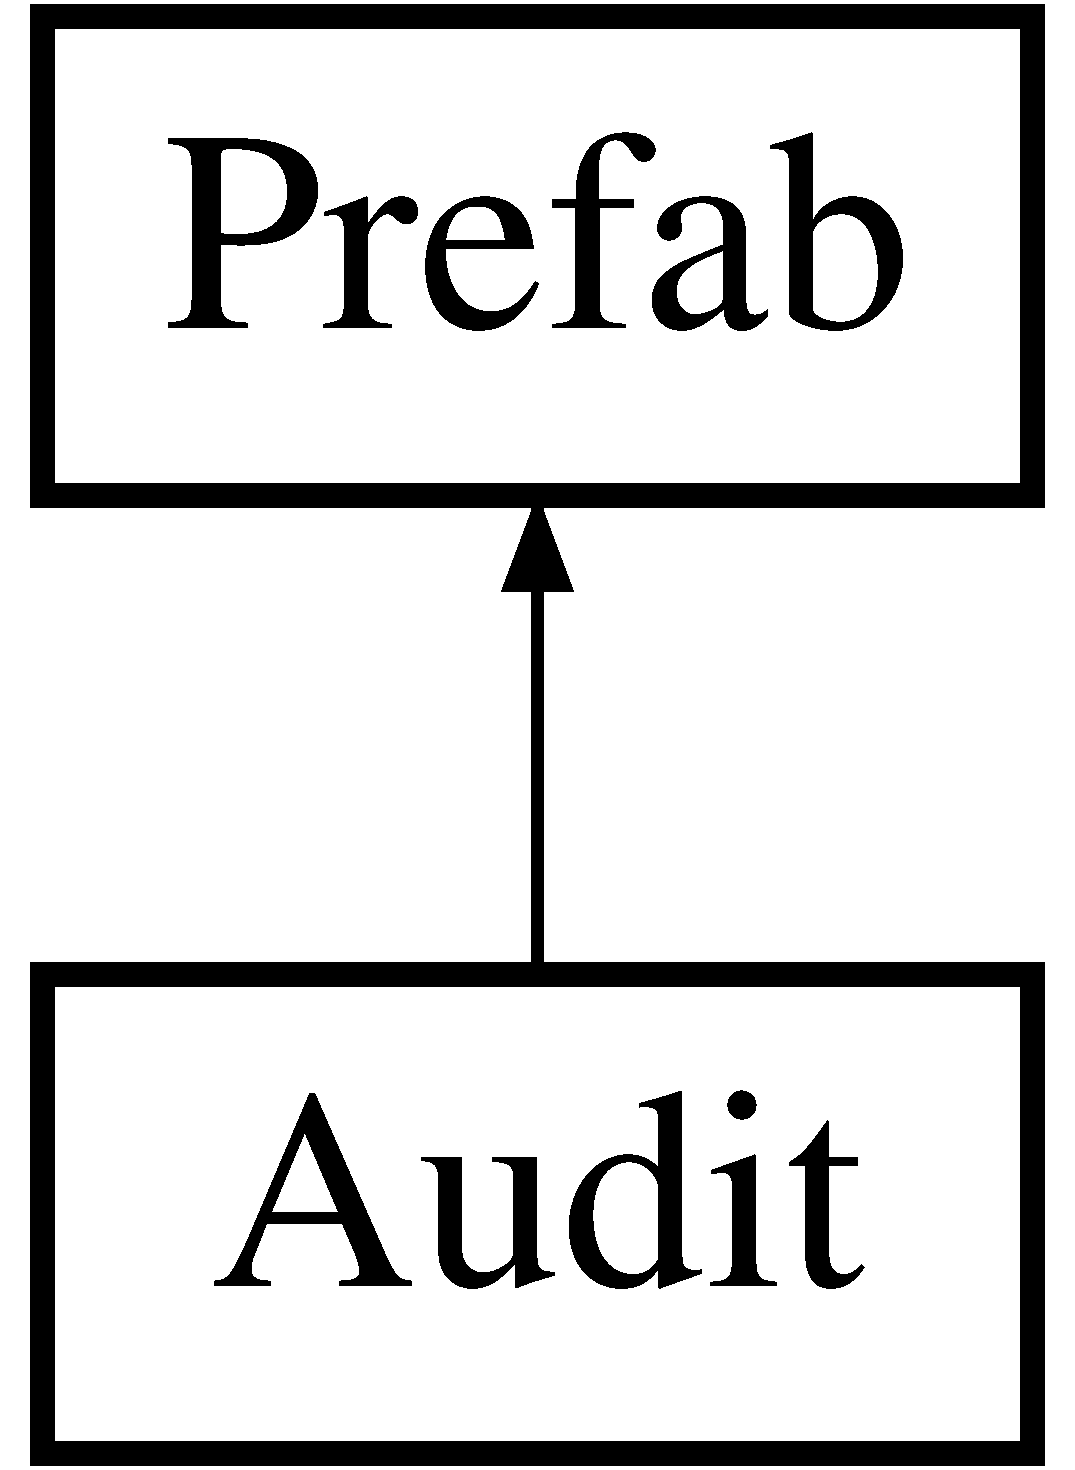
\includegraphics[height=2.000000cm]{class_audit}
\end{center}
\end{figure}
\subsection*{Public Member Functions}
\begin{DoxyCompactItemize}
\item 
\hyperlink{class_audit_aef8b9a57041dec7db0ff956bba1d8b3f}{url} (\$str)
\item 
\hyperlink{class_audit_a369b2fd023996c185845f4993d03f530}{email} (\$str, \$mx=T\+R\+UE)
\item 
\hyperlink{class_audit_a2c914582b13324bf624b1cd1763f258e}{ipv4} (\$addr)
\item 
\hyperlink{class_audit_a74a69adbf8a934eee039f323c864a508}{ipv6} (\$addr)
\item 
\hyperlink{class_audit_a9bb5536f5e8cfe33672340a407daa387}{isprivate} (\$addr)
\item 
\hyperlink{class_audit_a352a97e07f1d2ebb7dcc009da6c67825}{isreserved} (\$addr)
\item 
\hyperlink{class_audit_a421f0166ffee8171ee3948970abcecad}{ispublic} (\$addr)
\item 
\hyperlink{class_audit_ac6c1cda9920c8236cd00d10bffb2890f}{isdesktop} (\$agent=N\+U\+LL)
\item 
\hyperlink{class_audit_afbca2bf25d7295857c0e7b161ab21beb}{ismobile} (\$agent=N\+U\+LL)
\item 
\hyperlink{class_audit_a7d73389ff426668e83b171fd662018ad}{isbot} (\$agent=N\+U\+LL)
\item 
\hyperlink{class_audit_a80595e89a7b191abab586fcd73e54c6a}{mod10} (\$id)
\item 
\hyperlink{class_audit_a631df11fda2fb8e663e24f804c978367}{card} (\$id)
\item 
\hyperlink{class_audit_ac1c0abeb7a7ac6bf923e6e0abdfe336e}{entropy} (\$str)
\end{DoxyCompactItemize}
\subsection*{Data Fields}
{\bf }\par
\begin{DoxyCompactItemize}
\item 
\hypertarget{class_audit_a0a52494b8ebe7bc548e0ff67a81f717c}{}\label{class_audit_a0a52494b8ebe7bc548e0ff67a81f717c} 
const {\bfseries U\+A\+\_\+\+Mobile} =\textquotesingle{}android$\vert$blackberry$\vert$phone$\vert$ipod$\vert$palm$\vert$windows\textbackslash{}s+ce\textquotesingle{}
\item 
\hypertarget{class_audit_af48a17a5642de795ab0da730d87c6109}{}\label{class_audit_af48a17a5642de795ab0da730d87c6109} 
const {\bfseries U\+A\+\_\+\+Desktop} =\textquotesingle{}bsd$\vert$linux$\vert$os\textbackslash{}s+\mbox{[}x9\mbox{]}$\vert$solaris$\vert$windows\textquotesingle{}
\item 
\hypertarget{class_audit_a6c072917477cd06e254dda1a977406e6}{}\label{class_audit_a6c072917477cd06e254dda1a977406e6} 
const {\bfseries U\+A\+\_\+\+Bot} =\textquotesingle{}bot$\vert$crawl$\vert$slurp$\vert$spider\textquotesingle{}
\end{DoxyCompactItemize}

\subsection*{Additional Inherited Members}


\subsection{Detailed Description}
Data validator. 

Definition at line 24 of file audit.\+php.



\subsection{Member Function Documentation}
\hypertarget{class_audit_a631df11fda2fb8e663e24f804c978367}{}\label{class_audit_a631df11fda2fb8e663e24f804c978367} 
\index{Audit@{Audit}!card@{card}}
\index{card@{card}!Audit@{Audit}}
\subsubsection{\texorpdfstring{card()}{card()}}
{\footnotesize\ttfamily card (\begin{DoxyParamCaption}\item[{}]{\$id }\end{DoxyParamCaption})}

Return credit card type if number is valid \begin{DoxyReturn}{Returns}
string$\vert$\+F\+A\+L\+SE 
\end{DoxyReturn}

\begin{DoxyParams}{Parameters}
{\em \$id} & string \\
\hline
\end{DoxyParams}


Definition at line 158 of file audit.\+php.

\hypertarget{class_audit_a369b2fd023996c185845f4993d03f530}{}\label{class_audit_a369b2fd023996c185845f4993d03f530} 
\index{Audit@{Audit}!email@{email}}
\index{email@{email}!Audit@{Audit}}
\subsubsection{\texorpdfstring{email()}{email()}}
{\footnotesize\ttfamily email (\begin{DoxyParamCaption}\item[{}]{\$str,  }\item[{}]{\$mx = {\ttfamily TRUE} }\end{DoxyParamCaption})}

Return T\+R\+UE if string is a valid e-\/mail address; Check D\+NS MX records if specified \begin{DoxyReturn}{Returns}
bool 
\end{DoxyReturn}

\begin{DoxyParams}{Parameters}
{\em \$str} & string \\
\hline
{\em \$mx} & boolean \\
\hline
\end{DoxyParams}


Definition at line 49 of file audit.\+php.

\hypertarget{class_audit_ac1c0abeb7a7ac6bf923e6e0abdfe336e}{}\label{class_audit_ac1c0abeb7a7ac6bf923e6e0abdfe336e} 
\index{Audit@{Audit}!entropy@{entropy}}
\index{entropy@{entropy}!Audit@{Audit}}
\subsubsection{\texorpdfstring{entropy()}{entropy()}}
{\footnotesize\ttfamily entropy (\begin{DoxyParamCaption}\item[{}]{\$str }\end{DoxyParamCaption})}

Return entropy estimate of a password (N\+I\+ST 800-\/63) \begin{DoxyReturn}{Returns}
int$\vert$float 
\end{DoxyReturn}

\begin{DoxyParams}{Parameters}
{\em \$str} & string \\
\hline
\end{DoxyParams}


Definition at line 183 of file audit.\+php.

\hypertarget{class_audit_a2c914582b13324bf624b1cd1763f258e}{}\label{class_audit_a2c914582b13324bf624b1cd1763f258e} 
\index{Audit@{Audit}!ipv4@{ipv4}}
\index{ipv4@{ipv4}!Audit@{Audit}}
\subsubsection{\texorpdfstring{ipv4()}{ipv4()}}
{\footnotesize\ttfamily ipv4 (\begin{DoxyParamCaption}\item[{}]{\$addr }\end{DoxyParamCaption})}

Return T\+R\+UE if string is a valid I\+P\+V4 address \begin{DoxyReturn}{Returns}
bool 
\end{DoxyReturn}

\begin{DoxyParams}{Parameters}
{\em \$addr} & string \\
\hline
\end{DoxyParams}


Definition at line 60 of file audit.\+php.

\hypertarget{class_audit_a74a69adbf8a934eee039f323c864a508}{}\label{class_audit_a74a69adbf8a934eee039f323c864a508} 
\index{Audit@{Audit}!ipv6@{ipv6}}
\index{ipv6@{ipv6}!Audit@{Audit}}
\subsubsection{\texorpdfstring{ipv6()}{ipv6()}}
{\footnotesize\ttfamily ipv6 (\begin{DoxyParamCaption}\item[{}]{\$addr }\end{DoxyParamCaption})}

Return T\+R\+UE if string is a valid I\+P\+V6 address \begin{DoxyReturn}{Returns}
bool 
\end{DoxyReturn}

\begin{DoxyParams}{Parameters}
{\em \$addr} & string \\
\hline
\end{DoxyParams}


Definition at line 69 of file audit.\+php.

\hypertarget{class_audit_a7d73389ff426668e83b171fd662018ad}{}\label{class_audit_a7d73389ff426668e83b171fd662018ad} 
\index{Audit@{Audit}!isbot@{isbot}}
\index{isbot@{isbot}!Audit@{Audit}}
\subsubsection{\texorpdfstring{isbot()}{isbot()}}
{\footnotesize\ttfamily isbot (\begin{DoxyParamCaption}\item[{}]{\$agent = {\ttfamily NULL} }\end{DoxyParamCaption})}

Return T\+R\+UE if user agent is a \hyperlink{class_web}{Web} bot \begin{DoxyReturn}{Returns}
bool 
\end{DoxyReturn}

\begin{DoxyParams}{Parameters}
{\em \$agent} & string \\
\hline
\end{DoxyParams}


Definition at line 132 of file audit.\+php.

\hypertarget{class_audit_ac6c1cda9920c8236cd00d10bffb2890f}{}\label{class_audit_ac6c1cda9920c8236cd00d10bffb2890f} 
\index{Audit@{Audit}!isdesktop@{isdesktop}}
\index{isdesktop@{isdesktop}!Audit@{Audit}}
\subsubsection{\texorpdfstring{isdesktop()}{isdesktop()}}
{\footnotesize\ttfamily isdesktop (\begin{DoxyParamCaption}\item[{}]{\$agent = {\ttfamily NULL} }\end{DoxyParamCaption})}

Return T\+R\+UE if user agent is a desktop browser \begin{DoxyReturn}{Returns}
bool 
\end{DoxyReturn}

\begin{DoxyParams}{Parameters}
{\em \$agent} & string \\
\hline
\end{DoxyParams}


Definition at line 109 of file audit.\+php.

\hypertarget{class_audit_afbca2bf25d7295857c0e7b161ab21beb}{}\label{class_audit_afbca2bf25d7295857c0e7b161ab21beb} 
\index{Audit@{Audit}!ismobile@{ismobile}}
\index{ismobile@{ismobile}!Audit@{Audit}}
\subsubsection{\texorpdfstring{ismobile()}{ismobile()}}
{\footnotesize\ttfamily ismobile (\begin{DoxyParamCaption}\item[{}]{\$agent = {\ttfamily NULL} }\end{DoxyParamCaption})}

Return T\+R\+UE if user agent is a mobile device \begin{DoxyReturn}{Returns}
bool 
\end{DoxyReturn}

\begin{DoxyParams}{Parameters}
{\em \$agent} & string \\
\hline
\end{DoxyParams}


Definition at line 121 of file audit.\+php.

\hypertarget{class_audit_a9bb5536f5e8cfe33672340a407daa387}{}\label{class_audit_a9bb5536f5e8cfe33672340a407daa387} 
\index{Audit@{Audit}!isprivate@{isprivate}}
\index{isprivate@{isprivate}!Audit@{Audit}}
\subsubsection{\texorpdfstring{isprivate()}{isprivate()}}
{\footnotesize\ttfamily isprivate (\begin{DoxyParamCaption}\item[{}]{\$addr }\end{DoxyParamCaption})}

Return T\+R\+UE if IP address is within private range \begin{DoxyReturn}{Returns}
bool 
\end{DoxyReturn}

\begin{DoxyParams}{Parameters}
{\em \$addr} & string \\
\hline
\end{DoxyParams}


Definition at line 78 of file audit.\+php.

\hypertarget{class_audit_a421f0166ffee8171ee3948970abcecad}{}\label{class_audit_a421f0166ffee8171ee3948970abcecad} 
\index{Audit@{Audit}!ispublic@{ispublic}}
\index{ispublic@{ispublic}!Audit@{Audit}}
\subsubsection{\texorpdfstring{ispublic()}{ispublic()}}
{\footnotesize\ttfamily ispublic (\begin{DoxyParamCaption}\item[{}]{\$addr }\end{DoxyParamCaption})}

Return T\+R\+UE if IP address is neither private nor reserved \begin{DoxyReturn}{Returns}
bool 
\end{DoxyReturn}

\begin{DoxyParams}{Parameters}
{\em \$addr} & string \\
\hline
\end{DoxyParams}


Definition at line 98 of file audit.\+php.

\hypertarget{class_audit_a352a97e07f1d2ebb7dcc009da6c67825}{}\label{class_audit_a352a97e07f1d2ebb7dcc009da6c67825} 
\index{Audit@{Audit}!isreserved@{isreserved}}
\index{isreserved@{isreserved}!Audit@{Audit}}
\subsubsection{\texorpdfstring{isreserved()}{isreserved()}}
{\footnotesize\ttfamily isreserved (\begin{DoxyParamCaption}\item[{}]{\$addr }\end{DoxyParamCaption})}

Return T\+R\+UE if IP address is within reserved range \begin{DoxyReturn}{Returns}
bool 
\end{DoxyReturn}

\begin{DoxyParams}{Parameters}
{\em \$addr} & string \\
\hline
\end{DoxyParams}


Definition at line 88 of file audit.\+php.

\hypertarget{class_audit_a80595e89a7b191abab586fcd73e54c6a}{}\label{class_audit_a80595e89a7b191abab586fcd73e54c6a} 
\index{Audit@{Audit}!mod10@{mod10}}
\index{mod10@{mod10}!Audit@{Audit}}
\subsubsection{\texorpdfstring{mod10()}{mod10()}}
{\footnotesize\ttfamily mod10 (\begin{DoxyParamCaption}\item[{}]{\$id }\end{DoxyParamCaption})}

Return T\+R\+UE if specified ID has a valid (Luhn) Mod-\/10 check digit \begin{DoxyReturn}{Returns}
bool 
\end{DoxyReturn}

\begin{DoxyParams}{Parameters}
{\em \$id} & string \\
\hline
\end{DoxyParams}


Definition at line 143 of file audit.\+php.

\hypertarget{class_audit_aef8b9a57041dec7db0ff956bba1d8b3f}{}\label{class_audit_aef8b9a57041dec7db0ff956bba1d8b3f} 
\index{Audit@{Audit}!url@{url}}
\index{url@{url}!Audit@{Audit}}
\subsubsection{\texorpdfstring{url()}{url()}}
{\footnotesize\ttfamily url (\begin{DoxyParamCaption}\item[{}]{\$str }\end{DoxyParamCaption})}

Return T\+R\+UE if string is a valid U\+RL \begin{DoxyReturn}{Returns}
bool 
\end{DoxyReturn}

\begin{DoxyParams}{Parameters}
{\em \$str} & string \\
\hline
\end{DoxyParams}


Definition at line 38 of file audit.\+php.



The documentation for this class was generated from the following file\+:\begin{DoxyCompactItemize}
\item 
/\+Users/aplennevaux/\+G\+I\+T\+H\+U\+B/\+Visionary-\/website/src/vendor/bcosca/fatfree/lib/audit.\+php\end{DoxyCompactItemize}

\hypertarget{class_auth}{}\section{Auth Class Reference}
\label{class_auth}\index{Auth@{Auth}}


Authorization/authentication plug-\/in.  


\subsection*{Public Member Functions}
\begin{DoxyCompactItemize}
\item 
\hyperlink{class_auth_a6795c5b38d65b91cd9512fd1aea79577}{login} (\$id, \$pw, \$realm=N\+U\+LL)
\item 
\hyperlink{class_auth_ac76f1632910cb4c297b9244191530458}{basic} (\$func=N\+U\+LL)
\item 
\hyperlink{class_auth_a9ca59d2216de9a1756d9886e527b3971}{\+\_\+\+\_\+construct} (\$storage, array \$args=N\+U\+LL)
\end{DoxyCompactItemize}
\subsection*{Data Fields}
\begin{DoxyCompactItemize}
\item 
\hypertarget{class_auth_ace79db87eaeb4a62b8d0b4323f91ebe6}{}\label{class_auth_ace79db87eaeb4a62b8d0b4323f91ebe6} 
\hyperlink{class_auth_ace79db87eaeb4a62b8d0b4323f91ebe6}{\$mapper}
\begin{DoxyCompactList}\small\item\em Mapper object. \end{DoxyCompactList}\item 
\hypertarget{class_auth_a67e94494731d99ed23b123e95175bc10}{}\label{class_auth_a67e94494731d99ed23b123e95175bc10} 
\hyperlink{class_auth_a67e94494731d99ed23b123e95175bc10}{\$args}
\begin{DoxyCompactList}\small\item\em Storage options. \end{DoxyCompactList}\end{DoxyCompactItemize}
{\bf }\par
\begin{DoxyCompactItemize}
\item 
\hypertarget{class_auth_ab6a2feaefb83bee8bb8d4162543a4178}{}\label{class_auth_ab6a2feaefb83bee8bb8d4162543a4178} 
const {\bfseries E\+\_\+\+L\+D\+AP} =\textquotesingle{}L\+D\+AP connection failure\textquotesingle{}
\item 
\hypertarget{class_auth_a340cd055cd9bc3254658a9cf246313c7}{}\label{class_auth_a340cd055cd9bc3254658a9cf246313c7} 
const {\bfseries E\+\_\+\+S\+M\+TP} =\textquotesingle{}\hyperlink{class_s_m_t_p}{S\+M\+TP} connection failure\textquotesingle{}
\end{DoxyCompactItemize}

\subsection*{Protected Member Functions}
\begin{DoxyCompactItemize}
\item 
\hyperlink{class_auth_a81198296a350267473fdd52a525f1ccd}{\+\_\+jig} (\$id, \$pw, \$realm)
\item 
\hyperlink{class_auth_a4b51050fdae893312cb041b9074e1027}{\+\_\+mongo} (\$id, \$pw, \$realm)
\item 
\hyperlink{class_auth_a82093435675852de0fdcee08e43ceb74}{\+\_\+sql} (\$id, \$pw, \$realm)
\item 
\hyperlink{class_auth_a891591e9fc755d9d87903330b84d7e4f}{\+\_\+ldap} (\$id, \$pw)
\item 
\hyperlink{class_auth_af5d9f4a9f695edde6988b238a1759040}{\+\_\+smtp} (\$id, \$pw)
\end{DoxyCompactItemize}
\subsection*{Protected Attributes}
\begin{DoxyCompactItemize}
\item 
\hypertarget{class_auth_a23658d9b796eebdea4cee5c9f0046894}{}\label{class_auth_a23658d9b796eebdea4cee5c9f0046894} 
\hyperlink{class_auth_a23658d9b796eebdea4cee5c9f0046894}{\$storage}
\begin{DoxyCompactList}\small\item\em \hyperlink{class_auth}{Auth} storage. \end{DoxyCompactList}\end{DoxyCompactItemize}


\subsection{Detailed Description}
Authorization/authentication plug-\/in. 

Definition at line 24 of file auth.\+php.



\subsection{Constructor \& Destructor Documentation}
\hypertarget{class_auth_a9ca59d2216de9a1756d9886e527b3971}{}\label{class_auth_a9ca59d2216de9a1756d9886e527b3971} 
\index{Auth@{Auth}!\+\_\+\+\_\+construct@{\+\_\+\+\_\+construct}}
\index{\+\_\+\+\_\+construct@{\+\_\+\+\_\+construct}!Auth@{Auth}}
\subsubsection{\texorpdfstring{\+\_\+\+\_\+construct()}{\_\_construct()}}
{\footnotesize\ttfamily \+\_\+\+\_\+construct (\begin{DoxyParamCaption}\item[{}]{\$storage,  }\item[{array}]{\$args = {\ttfamily NULL} }\end{DoxyParamCaption})}

Instantiate class \begin{DoxyReturn}{Returns}
object 
\end{DoxyReturn}

\begin{DoxyParams}{Parameters}
{\em \$storage} & string$\vert$object \\
\hline
{\em \$args} & array \\
\hline
\end{DoxyParams}


Definition at line 229 of file auth.\+php.



\subsection{Member Function Documentation}
\hypertarget{class_auth_a81198296a350267473fdd52a525f1ccd}{}\label{class_auth_a81198296a350267473fdd52a525f1ccd} 
\index{Auth@{Auth}!\+\_\+jig@{\+\_\+jig}}
\index{\+\_\+jig@{\+\_\+jig}!Auth@{Auth}}
\subsubsection{\texorpdfstring{\+\_\+jig()}{\_jig()}}
{\footnotesize\ttfamily \+\_\+jig (\begin{DoxyParamCaption}\item[{}]{\$id,  }\item[{}]{\$pw,  }\item[{}]{\$realm }\end{DoxyParamCaption})\hspace{0.3cm}{\ttfamily [protected]}}

Jig storage handler \begin{DoxyReturn}{Returns}
bool 
\end{DoxyReturn}

\begin{DoxyParams}{Parameters}
{\em \$id} & string \\
\hline
{\em \$pw} & string \\
\hline
{\em \$realm} & string \\
\hline
\end{DoxyParams}


Definition at line 47 of file auth.\+php.

\hypertarget{class_auth_a891591e9fc755d9d87903330b84d7e4f}{}\label{class_auth_a891591e9fc755d9d87903330b84d7e4f} 
\index{Auth@{Auth}!\+\_\+ldap@{\+\_\+ldap}}
\index{\+\_\+ldap@{\+\_\+ldap}!Auth@{Auth}}
\subsubsection{\texorpdfstring{\+\_\+ldap()}{\_ldap()}}
{\footnotesize\ttfamily \+\_\+ldap (\begin{DoxyParamCaption}\item[{}]{\$id,  }\item[{}]{\$pw }\end{DoxyParamCaption})\hspace{0.3cm}{\ttfamily [protected]}}

L\+D\+AP storage handler \begin{DoxyReturn}{Returns}
bool 
\end{DoxyReturn}

\begin{DoxyParams}{Parameters}
{\em \$id} & string \\
\hline
{\em \$pw} & string \\
\hline
\end{DoxyParams}


Definition at line 117 of file auth.\+php.

\hypertarget{class_auth_a4b51050fdae893312cb041b9074e1027}{}\label{class_auth_a4b51050fdae893312cb041b9074e1027} 
\index{Auth@{Auth}!\+\_\+mongo@{\+\_\+mongo}}
\index{\+\_\+mongo@{\+\_\+mongo}!Auth@{Auth}}
\subsubsection{\texorpdfstring{\+\_\+mongo()}{\_mongo()}}
{\footnotesize\ttfamily \+\_\+mongo (\begin{DoxyParamCaption}\item[{}]{\$id,  }\item[{}]{\$pw,  }\item[{}]{\$realm }\end{DoxyParamCaption})\hspace{0.3cm}{\ttfamily [protected]}}

Mongo\+DB storage handler \begin{DoxyReturn}{Returns}
bool 
\end{DoxyReturn}

\begin{DoxyParams}{Parameters}
{\em \$id} & string \\
\hline
{\em \$pw} & string \\
\hline
{\em \$realm} & string \\
\hline
\end{DoxyParams}


Definition at line 73 of file auth.\+php.

\hypertarget{class_auth_af5d9f4a9f695edde6988b238a1759040}{}\label{class_auth_af5d9f4a9f695edde6988b238a1759040} 
\index{Auth@{Auth}!\+\_\+smtp@{\+\_\+smtp}}
\index{\+\_\+smtp@{\+\_\+smtp}!Auth@{Auth}}
\subsubsection{\texorpdfstring{\+\_\+smtp()}{\_smtp()}}
{\footnotesize\ttfamily \+\_\+smtp (\begin{DoxyParamCaption}\item[{}]{\$id,  }\item[{}]{\$pw }\end{DoxyParamCaption})\hspace{0.3cm}{\ttfamily [protected]}}

\hyperlink{class_s_m_t_p}{S\+M\+TP} storage handler \begin{DoxyReturn}{Returns}
bool 
\end{DoxyReturn}

\begin{DoxyParams}{Parameters}
{\em \$id} & string \\
\hline
{\em \$pw} & string \\
\hline
\end{DoxyParams}


Definition at line 140 of file auth.\+php.

\hypertarget{class_auth_a82093435675852de0fdcee08e43ceb74}{}\label{class_auth_a82093435675852de0fdcee08e43ceb74} 
\index{Auth@{Auth}!\+\_\+sql@{\+\_\+sql}}
\index{\+\_\+sql@{\+\_\+sql}!Auth@{Auth}}
\subsubsection{\texorpdfstring{\+\_\+sql()}{\_sql()}}
{\footnotesize\ttfamily \+\_\+sql (\begin{DoxyParamCaption}\item[{}]{\$id,  }\item[{}]{\$pw,  }\item[{}]{\$realm }\end{DoxyParamCaption})\hspace{0.3cm}{\ttfamily [protected]}}

S\+QL storage handler \begin{DoxyReturn}{Returns}
bool 
\end{DoxyReturn}

\begin{DoxyParams}{Parameters}
{\em \$id} & string \\
\hline
{\em \$pw} & string \\
\hline
{\em \$realm} & string \\
\hline
\end{DoxyParams}


Definition at line 92 of file auth.\+php.

\hypertarget{class_auth_ac76f1632910cb4c297b9244191530458}{}\label{class_auth_ac76f1632910cb4c297b9244191530458} 
\index{Auth@{Auth}!basic@{basic}}
\index{basic@{basic}!Auth@{Auth}}
\subsubsection{\texorpdfstring{basic()}{basic()}}
{\footnotesize\ttfamily basic (\begin{DoxyParamCaption}\item[{}]{\$func = {\ttfamily NULL} }\end{DoxyParamCaption})}

H\+T\+TP basic auth mechanism \begin{DoxyReturn}{Returns}
bool 
\end{DoxyReturn}

\begin{DoxyParams}{Parameters}
{\em \$func} & callback \\
\hline
\end{DoxyParams}


Definition at line 197 of file auth.\+php.

\hypertarget{class_auth_a6795c5b38d65b91cd9512fd1aea79577}{}\label{class_auth_a6795c5b38d65b91cd9512fd1aea79577} 
\index{Auth@{Auth}!login@{login}}
\index{login@{login}!Auth@{Auth}}
\subsubsection{\texorpdfstring{login()}{login()}}
{\footnotesize\ttfamily login (\begin{DoxyParamCaption}\item[{}]{\$id,  }\item[{}]{\$pw,  }\item[{}]{\$realm = {\ttfamily NULL} }\end{DoxyParamCaption})}

Login auth mechanism \begin{DoxyReturn}{Returns}
bool 
\end{DoxyReturn}

\begin{DoxyParams}{Parameters}
{\em \$id} & string \\
\hline
{\em \$pw} & string \\
\hline
{\em \$realm} & string \\
\hline
\end{DoxyParams}


Definition at line 188 of file auth.\+php.



The documentation for this class was generated from the following file\+:\begin{DoxyCompactItemize}
\item 
/\+Users/aplennevaux/\+G\+I\+T\+H\+U\+B/\+Visionary-\/website/src/vendor/bcosca/fatfree/lib/auth.\+php\end{DoxyCompactItemize}

\hypertarget{class_base}{}\section{Base Class Reference}
\label{class_base}\index{Base@{Base}}


\hyperlink{class_base}{Base} structure.  


Inheritance diagram for Base\+:\begin{figure}[H]
\begin{center}
\leavevmode
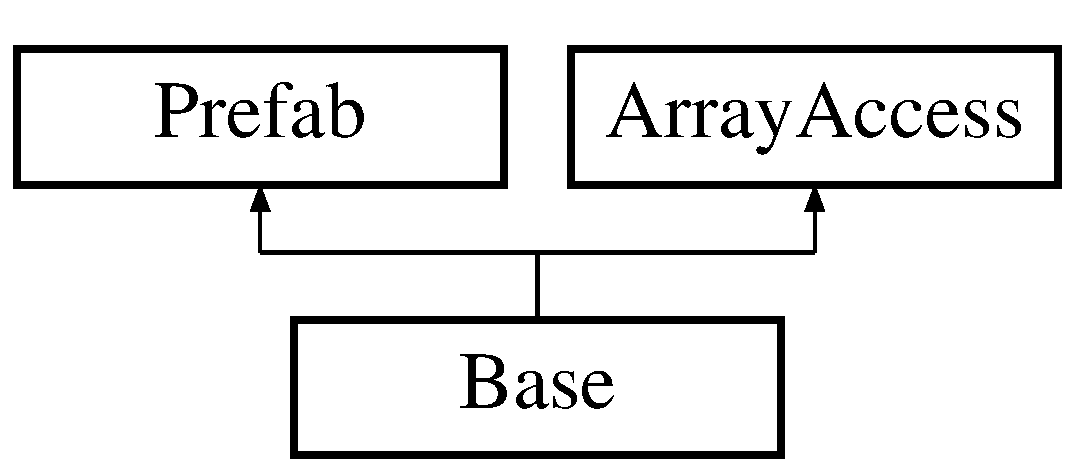
\includegraphics[height=2.000000cm]{class_base}
\end{center}
\end{figure}
\subsection*{Public Member Functions}
\begin{DoxyCompactItemize}
\item 
\hyperlink{class_base_aada982ed0466e5ed14d4fcbe22c61840}{sync} (\$key)
\item 
\hyperlink{class_base_a9f2a5290b60008d473e1c9e38f1465d0}{build} (\$url, \$args=\mbox{[}$\,$\mbox{]})
\item 
\hyperlink{class_base_a222997c88655e69eb1bb3a18147ddc3d}{alias} (\$name, \$params=\mbox{[}$\,$\mbox{]}, \$query=N\+U\+LL)
\item 
\hyperlink{class_base_a4d0e49aacf195439c437277b22a81062}{parse} (\$str)
\item 
\hyperlink{class_base_af206a5f3197cfe2acbbb071ec086b710}{compile} (\$str)
\item 
\& \hyperlink{class_base_aee913b6f1b4e910dc64485c4d8e48b15}{ref} (\$key, \$add=T\+R\+UE, \&\$var=N\+U\+LL)
\item 
\hyperlink{class_base_a28497caad131119319e31168c38713b6}{exists} (\$key, \&\$val=N\+U\+LL)
\item 
\hyperlink{class_base_a7de02315df24d7ef20a0bd441060d6d2}{devoid} (\$key, \&\$val=N\+U\+LL)
\item 
\hyperlink{class_base_a845297666b2c78affb9fa78605ebf93e}{set} (\$key, \$val, \$ttl=0)
\item 
\hyperlink{class_base_a17baee8d5275e5926004818839f9d838}{get} (\$key, \$args=N\+U\+LL)
\item 
\hyperlink{class_base_a10a949ef75de6c82c98ac555f371ba83}{clear} (\$key)
\item 
\hyperlink{class_base_a1e33118c04d4a7df9336e02db8f8d663}{checked} (\$key)
\item 
\hyperlink{class_base_a6cdd645b49b8ec6bd1bebe80074f98fb}{visible} (\$obj, \$key)
\item 
\hyperlink{class_base_aa4d056d44b4c50924926f9d40cdb9bf2}{mset} (array \$vars, \$prefix=\textquotesingle{}\textquotesingle{}, \$ttl=0)
\item 
\hyperlink{class_base_a9492bc2587be1faa2fa7e69d2a89a53e}{hive} ()
\item 
\hyperlink{class_base_a9051a0cda0ec6cae19cbd32e3945f31a}{copy} (\$src, \$dst)
\item 
\hyperlink{class_base_ac750abed7c77c34dab7894d272a2a293}{concat} (\$key, \$val)
\item 
\hyperlink{class_base_a0b0020960192ed3b1d87f4c1a2587373}{flip} (\$key)
\item 
\hyperlink{class_base_aef81a11cc1b68233d80e63bcf6fa94f3}{push} (\$key, \$val)
\item 
\hyperlink{class_base_a0a5ec8de186492bebff151ad40b17fa4}{pop} (\$key)
\item 
\hyperlink{class_base_a44e8f53ad45c8f0caa4e438285d08a49}{unshift} (\$key, \$val)
\item 
\hyperlink{class_base_a4ddb1b90cf267ea505ec59db4c6f5134}{shift} (\$key)
\item 
\hyperlink{class_base_a9dc15a0b65021967dad733868514f2a3}{merge} (\$key, \$src, \$keep=F\+A\+L\+SE)
\item 
\hyperlink{class_base_adab2e4455e35467d6012ceaf488a3744}{extend} (\$key, \$src, \$keep=F\+A\+L\+SE)
\item 
\hyperlink{class_base_a052692dd304d0f28451a8fc601fa277e}{fixslashes} (\$str)
\item 
\hyperlink{class_base_ac7b410d4c7145630a45e608d465bb1b5}{split} (\$str, \$noempty=T\+R\+UE)
\item 
\hyperlink{class_base_adb7cb366d6c6e4d4338bc35e76dfaf67}{stringify} (\$arg, array \$stack=N\+U\+LL)
\item 
\hyperlink{class_base_a2f39631e6920b33e0e88713de4566bdc}{csv} (array \$args)
\item 
\hyperlink{class_base_ad8ac953e9fcd497f1ce693e7639911a5}{camelcase} (\$str)
\item 
\hyperlink{class_base_a28e7ef7f4daed47ec1d65760c0a85c27}{snakecase} (\$str)
\item 
\hyperlink{class_base_a94648b79713b75bf4b68864e4f916df4}{sign} (\$num)
\item 
\hyperlink{class_base_abb0deeb7aea6b11961c802cddd6f5925}{extract} (\$arr, \$prefix)
\item 
\hyperlink{class_base_a8906c778c90cf5be4c1d76cd005945c5}{constants} (\$class, \$prefix=\textquotesingle{}\textquotesingle{})
\item 
\hyperlink{class_base_aea8db0058c00fd2bc1351ddb2ebf3191}{hash} (\$str)
\item 
\hyperlink{class_base_a3b0a49639cd46ae1a3a817552b10e242}{base64} (\$data, \$mime)
\item 
\hyperlink{class_base_a27ad9a200330b2a3e71f8fa5df0f3397}{encode} (\$str)
\item 
\hyperlink{class_base_a4afbb486f4a5ff5a8170c832f5997986}{decode} (\$str)
\item 
\hyperlink{class_base_a17f774c561c4ac4a77f691bd98d5b647}{recursive} (\$arg, \$func, \$stack=\mbox{[}$\,$\mbox{]})
\item 
\hyperlink{class_base_aaaeb3a6da8c7c370705a33e599c3144a}{clean} (\$arg, \$tags=N\+U\+LL)
\item 
\hyperlink{class_base_aa5b63d859ddc3953cc72877b834beb53}{scrub} (\&\$var, \$tags=N\+U\+LL)
\item 
\hyperlink{class_base_afe083716d50b3fb4057e519961b9235c}{format} ()
\item 
\hyperlink{class_base_aeff6ba9b2402e9a6e39c424452f8ffb1}{language} (\$code)
\item 
\hyperlink{class_base_a084dcc9ed975d967d44aeafc628db4da}{lexicon} (\$path, \$ttl=0)
\item 
\hyperlink{class_base_a8f26410af8419317fe83d822e12c18f0}{serialize} (\$arg)
\item 
\hyperlink{class_base_ad07703b75ad394aac9592c2f7684f87e}{unserialize} (\$arg)
\item 
\hyperlink{class_base_a4505aab5ca6dd00d047da06786883df2}{status} (\$code)
\item 
\hyperlink{class_base_a11de9ffc2348b9090fbcd40fe00259ab}{expire} (\$secs=0)
\item 
\hyperlink{class_base_a77f6a261d70e66c7b7273774832482dc}{agent} ()
\item 
\hyperlink{class_base_a73a8e42630137b1b11246d16d7cd23d5}{ajax} ()
\item 
\hyperlink{class_base_a197bae3714812901860bd006b00f91de}{ip} ()
\item 
\hyperlink{class_base_a83230924155c911fd8db8f0619ced19a}{trace} (array \$trace=N\+U\+LL, \$\hyperlink{class_base_afe083716d50b3fb4057e519961b9235c}{format}=T\+R\+UE)
\item 
\hyperlink{class_base_aa73cf9e2c791864c9baf4c2d55b5f68b}{error} (\$code, \$text=\textquotesingle{}\textquotesingle{}, array \$\hyperlink{class_base_a83230924155c911fd8db8f0619ced19a}{trace}=N\+U\+LL, \$level=0)
\item 
\hyperlink{class_base_a37955584341e20d695a2dea982e3e192}{mock} (\$pattern, array \$args=N\+U\+LL, array \$headers=N\+U\+LL, \$body=N\+U\+LL)
\item 
\hyperlink{class_base_a369026a3cb8f321eadc19535ee308b2d}{route} (\$pattern, \$handler, \$ttl=0, \$kbps=0)
\item 
\hyperlink{class_base_a5a8efc7bc5d742984142bbcd2266128d}{reroute} (\$url=N\+U\+LL, \$permanent=F\+A\+L\+SE)
\item 
\hyperlink{class_base_ad64de620e7d21824d5f36dad0fb75945}{map} (\$url, \$class, \$ttl=0, \$kbps=0)
\item 
\hyperlink{class_base_aabd48f745ba0f411f2a62460d5d10fba}{redirect} (\$pattern, \$url, \$permanent=T\+R\+UE)
\item 
\hyperlink{class_base_a3e27c86c02a50a6906d9d92337d7437d}{blacklisted} (\$\hyperlink{class_base_a197bae3714812901860bd006b00f91de}{ip})
\item 
\hyperlink{class_base_abc7b4470fe464baa2b35ec59e1a3ee3a}{mask} (\$pattern, \$url=N\+U\+LL)
\item 
\hyperlink{class_base_afb0fafe7e02a3ae1993c01c19fad2bae}{run} ()
\item 
\hyperlink{class_base_ac0839746f9fe00ea683310b3af59c671}{until} (\$func, \$args=N\+U\+LL, \$timeout=60)
\item 
\hyperlink{class_base_a0b3225a00a2350b06234860096d5178a}{abort} ()
\item 
\hyperlink{class_base_a669bbc5855d5fc5ff1959819fd8a987d}{grab} (\$func, \$args=N\+U\+LL)
\item 
\hyperlink{class_base_a58d9a02809fd387d8ed8ace64e10628e}{call} (\$func, \$args=N\+U\+LL, \$hooks=\textquotesingle{}\textquotesingle{})
\item 
\hyperlink{class_base_ab92ef3c41964ec3291278fefb47d16f5}{chain} (\$funcs, \$args=N\+U\+LL)
\item 
\hyperlink{class_base_aeae41eb437d4e24660a712e05240515d}{relay} (\$funcs, \$args=N\+U\+LL)
\item 
\hyperlink{class_base_a9b5adda44e6db1d1f45cf1e4a6be5ce1}{config} (\$file, \$allow=F\+A\+L\+SE)
\item 
\hyperlink{class_base_aee63f67e17f2fce3781b9199e98025fb}{mutex} (\$id, \$func, \$args=N\+U\+LL)
\item 
\hyperlink{class_base_a7dbce4917d643c341f1c072f484329c1}{read} (\$file, \$lf=F\+A\+L\+SE)
\item 
\hyperlink{class_base_afb51e542cbff9f00cc964ac9bd6eecb5}{write} (\$file, \$data, \$append=F\+A\+L\+SE)
\item 
\hyperlink{class_base_a9e02fb072a50fb8358713128b41ba417}{highlight} (\$text)
\item 
\hyperlink{class_base_a238c9a8c7839b0773ee92327c86d3438}{dump} (\$expr)
\item 
\hyperlink{class_base_a83965c040afee15a85c5085b56626d80}{rel} (\$url)
\item 
\hyperlink{class_base_adc7d192011936335400f5baffa3c2667}{unload} (\$cwd)
\item 
\hyperlink{class_base_a16da5af940f99a0df550a7f7c7c5d4e4}{offsetexists} (\$key)
\item 
\hyperlink{class_base_a67693a9cff0abdfbbd353c36c00fb8d3}{offsetset} (\$key, \$val)
\item 
\& \hyperlink{class_base_a4736f7355697c49bcd06b643b4077e8a}{offsetget} (\$key)
\item 
\hyperlink{class_base_a414cd1cb3c09fc06e5e83502f6309dde}{offsetunset} (\$key)
\item 
\hyperlink{class_base_ae858fed7cd2822fbceac154138b68baa}{\+\_\+\+\_\+isset} (\$key)
\item 
\hyperlink{class_base_ae5e0d9ea041c1957ef04189b0b29657c}{\+\_\+\+\_\+set} (\$key, \$val)
\item 
\& \hyperlink{class_base_ae23a2c24bd42a7be642cdb71b58dbc5a}{\+\_\+\+\_\+get} (\$key)
\item 
\hyperlink{class_base_a41af7dd29c879b4c30978876ebdf4ba7}{\+\_\+\+\_\+unset} (\$key)
\item 
\hyperlink{class_base_a12381dd8315ac26000fdf6b9b0735321}{\+\_\+\+\_\+call} (\$key, \$args)
\item 
\hypertarget{class_base_a095c5d389db211932136b53f25f39685}{}\label{class_base_a095c5d389db211932136b53f25f39685} 
\hyperlink{class_base_a095c5d389db211932136b53f25f39685}{\+\_\+\+\_\+construct} ()
\begin{DoxyCompactList}\small\item\em Bootstrap. \end{DoxyCompactList}\end{DoxyCompactItemize}
\subsection*{Data Fields}
\begin{DoxyCompactItemize}
\item 
\hypertarget{class_base_a4a494a8977b10f1b9980faadf3ea0fc2}{}\label{class_base_a4a494a8977b10f1b9980faadf3ea0fc2} 
const \hyperlink{class_base_a4a494a8977b10f1b9980faadf3ea0fc2}{G\+L\+O\+B\+A\+LS} =\textquotesingle{}G\+ET$\vert$P\+O\+ST$\vert$C\+O\+O\+K\+IE$\vert$R\+E\+Q\+U\+E\+ST$\vert$S\+E\+S\+S\+I\+ON$\vert$F\+I\+L\+ES$\vert$S\+E\+R\+V\+ER$\vert$E\+NV\textquotesingle{}
\begin{DoxyCompactList}\small\item\em Mapped P\+HP globals. \end{DoxyCompactList}\item 
\hypertarget{class_base_a43552934268bce7080a8a0dfdab5ff48}{}\label{class_base_a43552934268bce7080a8a0dfdab5ff48} 
const \hyperlink{class_base_a43552934268bce7080a8a0dfdab5ff48}{V\+E\+R\+BS} =\textquotesingle{}G\+ET$\vert$H\+E\+AD$\vert$P\+O\+ST$\vert$P\+UT$\vert$P\+A\+T\+CH$\vert$D\+E\+L\+E\+TE$\vert$C\+O\+N\+N\+E\+CT\textquotesingle{}
\begin{DoxyCompactList}\small\item\em H\+T\+TP verbs. \end{DoxyCompactList}\item 
\hypertarget{class_base_a4eea605dd8e0b6a69464ec041dc9872a}{}\label{class_base_a4eea605dd8e0b6a69464ec041dc9872a} 
const \hyperlink{class_base_a4eea605dd8e0b6a69464ec041dc9872a}{M\+O\+DE} =0755
\begin{DoxyCompactList}\small\item\em Default directory permissions. \end{DoxyCompactList}\item 
\hypertarget{class_base_ad3c2e05f38fee8ac8cdc370fd4c84941}{}\label{class_base_ad3c2e05f38fee8ac8cdc370fd4c84941} 
const \hyperlink{class_base_ad3c2e05f38fee8ac8cdc370fd4c84941}{C\+SS} =\textquotesingle{}code.\+css\textquotesingle{}
\begin{DoxyCompactList}\small\item\em Syntax highlighting stylesheet. \end{DoxyCompactList}\item 
\hypertarget{class_base_a8834b0851b05d161c207a7d2e5dca9bd}{}\label{class_base_a8834b0851b05d161c207a7d2e5dca9bd} 
\hyperlink{class_base_a8834b0851b05d161c207a7d2e5dca9bd}{\$init}
\begin{DoxyCompactList}\small\item\em Initial settings. \end{DoxyCompactList}\item 
\hypertarget{class_base_a8856d0a49881ef8e0a6d205d37d4a7af}{}\label{class_base_a8856d0a49881ef8e0a6d205d37d4a7af} 
\hyperlink{class_base_a8856d0a49881ef8e0a6d205d37d4a7af}{\$languages}
\begin{DoxyCompactList}\small\item\em Language lookup sequence. \end{DoxyCompactList}\item 
\hypertarget{class_base_a0aa2d1acd291d3fedc1a3617d716e28e}{}\label{class_base_a0aa2d1acd291d3fedc1a3617d716e28e} 
\hyperlink{class_base_a0aa2d1acd291d3fedc1a3617d716e28e}{\$fallback} =\textquotesingle{}en\textquotesingle{}
\begin{DoxyCompactList}\small\item\em Default fallback language. \end{DoxyCompactList}\end{DoxyCompactItemize}
{\bf }\par
\begin{DoxyCompactItemize}
\item 
\hypertarget{class_base_a037d2e8a6e9d6f5c55e8b24e3faa5189}{}\label{class_base_a037d2e8a6e9d6f5c55e8b24e3faa5189} 
const {\bfseries P\+A\+C\+K\+A\+GE} =\textquotesingle{}Fat-\/Free Framework\textquotesingle{}
\item 
\hypertarget{class_base_af71005841ce53adac00581ab0ba24c1f}{}\label{class_base_af71005841ce53adac00581ab0ba24c1f} 
const {\bfseries V\+E\+R\+S\+I\+ON} =\textquotesingle{}3.\+6.\+0-\/Release\textquotesingle{}
\end{DoxyCompactItemize}

{\bf }\par
\begin{DoxyCompactItemize}
\item 
\hypertarget{class_base_a42c03aab8b513fd2992aeb7820003ad1}{}\label{class_base_a42c03aab8b513fd2992aeb7820003ad1} 
const {\bfseries H\+T\+T\+P\+\_\+100} =\textquotesingle{}Continue\textquotesingle{}
\item 
\hypertarget{class_base_a3e91894cd6ca5dcd2cdbc4e658328dbe}{}\label{class_base_a3e91894cd6ca5dcd2cdbc4e658328dbe} 
const {\bfseries H\+T\+T\+P\+\_\+101} =\textquotesingle{}Switching Protocols\textquotesingle{}
\item 
\hypertarget{class_base_ae0a2cfd13da12e121cd5cd44cdba63f1}{}\label{class_base_ae0a2cfd13da12e121cd5cd44cdba63f1} 
const {\bfseries H\+T\+T\+P\+\_\+200} =\textquotesingle{}OK\textquotesingle{}
\item 
\hypertarget{class_base_a5a183af6b7b3d27eadc14a92cc1a8f52}{}\label{class_base_a5a183af6b7b3d27eadc14a92cc1a8f52} 
const {\bfseries H\+T\+T\+P\+\_\+201} =\textquotesingle{}Created\textquotesingle{}
\item 
\hypertarget{class_base_a58dd15c950afe66a5723a02d296e8ef3}{}\label{class_base_a58dd15c950afe66a5723a02d296e8ef3} 
const {\bfseries H\+T\+T\+P\+\_\+202} =\textquotesingle{}Accepted\textquotesingle{}
\item 
\hypertarget{class_base_a6829270d25c830b55a9399c8c2f4c64d}{}\label{class_base_a6829270d25c830b55a9399c8c2f4c64d} 
const {\bfseries H\+T\+T\+P\+\_\+203} =\textquotesingle{}Non-\/Authorative Information\textquotesingle{}
\item 
\hypertarget{class_base_afe27bd4b405e5b231f7391a6ad27305d}{}\label{class_base_afe27bd4b405e5b231f7391a6ad27305d} 
const {\bfseries H\+T\+T\+P\+\_\+204} =\textquotesingle{}No Content\textquotesingle{}
\item 
\hypertarget{class_base_a6abfa0503972e8adc8901aac33e3ba82}{}\label{class_base_a6abfa0503972e8adc8901aac33e3ba82} 
const {\bfseries H\+T\+T\+P\+\_\+205} =\textquotesingle{}Reset Content\textquotesingle{}
\item 
\hypertarget{class_base_a58e0f63fd99ed0ea3e7e60d6ad3b945a}{}\label{class_base_a58e0f63fd99ed0ea3e7e60d6ad3b945a} 
const {\bfseries H\+T\+T\+P\+\_\+206} =\textquotesingle{}Partial Content\textquotesingle{}
\item 
\hypertarget{class_base_adafda22dbd720503d24641dd6233d288}{}\label{class_base_adafda22dbd720503d24641dd6233d288} 
const {\bfseries H\+T\+T\+P\+\_\+300} =\textquotesingle{}Multiple Choices\textquotesingle{}
\item 
\hypertarget{class_base_a6c5ed14921b8f4e396f4efe351b7cf17}{}\label{class_base_a6c5ed14921b8f4e396f4efe351b7cf17} 
const {\bfseries H\+T\+T\+P\+\_\+301} =\textquotesingle{}Moved Permanently\textquotesingle{}
\item 
\hypertarget{class_base_a6c27583e94a43460f3a53bc8d52928ed}{}\label{class_base_a6c27583e94a43460f3a53bc8d52928ed} 
const {\bfseries H\+T\+T\+P\+\_\+302} =\textquotesingle{}Found\textquotesingle{}
\item 
\hypertarget{class_base_ad1e133ece2bc42ef9f254c9816cc095b}{}\label{class_base_ad1e133ece2bc42ef9f254c9816cc095b} 
const {\bfseries H\+T\+T\+P\+\_\+303} =\textquotesingle{}See Other\textquotesingle{}
\item 
\hypertarget{class_base_abdb84279eb4c2ac564c82aa6e6b33304}{}\label{class_base_abdb84279eb4c2ac564c82aa6e6b33304} 
const {\bfseries H\+T\+T\+P\+\_\+304} =\textquotesingle{}Not Modified\textquotesingle{}
\item 
\hypertarget{class_base_a71b15cf5ca7eca4fcb95a65d9ef4591e}{}\label{class_base_a71b15cf5ca7eca4fcb95a65d9ef4591e} 
const {\bfseries H\+T\+T\+P\+\_\+305} =\textquotesingle{}Use Proxy\textquotesingle{}
\item 
\hypertarget{class_base_a8da1214deb6446d70f581c2019cfdbee}{}\label{class_base_a8da1214deb6446d70f581c2019cfdbee} 
const {\bfseries H\+T\+T\+P\+\_\+307} =\textquotesingle{}Temporary Redirect\textquotesingle{}
\item 
\hypertarget{class_base_a9bc01f248df88512037bd8ccb3bc62cf}{}\label{class_base_a9bc01f248df88512037bd8ccb3bc62cf} 
const {\bfseries H\+T\+T\+P\+\_\+400} =\textquotesingle{}Bad Request\textquotesingle{}
\item 
\hypertarget{class_base_a5edf9bc886987f75d84fa9a259fbff15}{}\label{class_base_a5edf9bc886987f75d84fa9a259fbff15} 
const {\bfseries H\+T\+T\+P\+\_\+401} =\textquotesingle{}Unauthorized\textquotesingle{}
\item 
\hypertarget{class_base_aa6565d2b492ee606d53edce743d5c71d}{}\label{class_base_aa6565d2b492ee606d53edce743d5c71d} 
const {\bfseries H\+T\+T\+P\+\_\+402} =\textquotesingle{}Payment Required\textquotesingle{}
\item 
\hypertarget{class_base_a026a0a02c60785631930a6b6a7dfa779}{}\label{class_base_a026a0a02c60785631930a6b6a7dfa779} 
const {\bfseries H\+T\+T\+P\+\_\+403} =\textquotesingle{}Forbidden\textquotesingle{}
\item 
\hypertarget{class_base_ab15b06b5211e7c1d62dbfefdd2f48fae}{}\label{class_base_ab15b06b5211e7c1d62dbfefdd2f48fae} 
const {\bfseries H\+T\+T\+P\+\_\+404} =\textquotesingle{}Not Found\textquotesingle{}
\item 
\hypertarget{class_base_ac8f37841b9501862ab4436188e6ef52c}{}\label{class_base_ac8f37841b9501862ab4436188e6ef52c} 
const {\bfseries H\+T\+T\+P\+\_\+405} =\textquotesingle{}Method Not Allowed\textquotesingle{}
\item 
\hypertarget{class_base_ac89c0f949c653c14eabf66cf51914f7a}{}\label{class_base_ac89c0f949c653c14eabf66cf51914f7a} 
const {\bfseries H\+T\+T\+P\+\_\+406} =\textquotesingle{}Not Acceptable\textquotesingle{}
\item 
\hypertarget{class_base_aa2744fa255e0fde11c39044a4f39218f}{}\label{class_base_aa2744fa255e0fde11c39044a4f39218f} 
const {\bfseries H\+T\+T\+P\+\_\+407} =\textquotesingle{}Proxy Authentication Required\textquotesingle{}
\item 
\hypertarget{class_base_ad478a80358a910b447fe9a8f0fe3e5f3}{}\label{class_base_ad478a80358a910b447fe9a8f0fe3e5f3} 
const {\bfseries H\+T\+T\+P\+\_\+408} =\textquotesingle{}Request Timeout\textquotesingle{}
\item 
\hypertarget{class_base_a14c4dd15ae82f4276945fe8ca3587425}{}\label{class_base_a14c4dd15ae82f4276945fe8ca3587425} 
const {\bfseries H\+T\+T\+P\+\_\+409} =\textquotesingle{}Conflict\textquotesingle{}
\item 
\hypertarget{class_base_a6ecb7b05cfc5c946b48c517f4cd1eb1e}{}\label{class_base_a6ecb7b05cfc5c946b48c517f4cd1eb1e} 
const {\bfseries H\+T\+T\+P\+\_\+410} =\textquotesingle{}Gone\textquotesingle{}
\item 
\hypertarget{class_base_a5fd3f7b58e313d50de57055da35b8c34}{}\label{class_base_a5fd3f7b58e313d50de57055da35b8c34} 
const {\bfseries H\+T\+T\+P\+\_\+411} =\textquotesingle{}Length Required\textquotesingle{}
\item 
\hypertarget{class_base_ab3afa21eeb61eec4bec88e01faa33a83}{}\label{class_base_ab3afa21eeb61eec4bec88e01faa33a83} 
const {\bfseries H\+T\+T\+P\+\_\+412} =\textquotesingle{}Precondition Failed\textquotesingle{}
\item 
\hypertarget{class_base_a45f0b1f7c9cf100d85d99d35122be993}{}\label{class_base_a45f0b1f7c9cf100d85d99d35122be993} 
const {\bfseries H\+T\+T\+P\+\_\+413} =\textquotesingle{}Request Entity Too Large\textquotesingle{}
\item 
\hypertarget{class_base_a3bc4a9f6ae41b35db4ef4cb6c3c81dc0}{}\label{class_base_a3bc4a9f6ae41b35db4ef4cb6c3c81dc0} 
const {\bfseries H\+T\+T\+P\+\_\+414} =\textquotesingle{}Request-\/U\+RI Too Long\textquotesingle{}
\item 
\hypertarget{class_base_a5d89cd8370f685b1f3e6e269687adc45}{}\label{class_base_a5d89cd8370f685b1f3e6e269687adc45} 
const {\bfseries H\+T\+T\+P\+\_\+415} =\textquotesingle{}Unsupported Media Type\textquotesingle{}
\item 
\hypertarget{class_base_a38e6c727e49a57b0d54d558ee6c42577}{}\label{class_base_a38e6c727e49a57b0d54d558ee6c42577} 
const {\bfseries H\+T\+T\+P\+\_\+416} =\textquotesingle{}Requested Range Not Satisfiable\textquotesingle{}
\item 
\hypertarget{class_base_adad1d3f1ac9914076661124ac1125344}{}\label{class_base_adad1d3f1ac9914076661124ac1125344} 
const {\bfseries H\+T\+T\+P\+\_\+417} =\textquotesingle{}Expectation Failed\textquotesingle{}
\item 
\hypertarget{class_base_a33889bdfdb2d12c842493341cd16851b}{}\label{class_base_a33889bdfdb2d12c842493341cd16851b} 
const {\bfseries H\+T\+T\+P\+\_\+500} =\textquotesingle{}Internal Server Error\textquotesingle{}
\item 
\hypertarget{class_base_a87cea373c6e56aaf7a228e510ba556ae}{}\label{class_base_a87cea373c6e56aaf7a228e510ba556ae} 
const {\bfseries H\+T\+T\+P\+\_\+501} =\textquotesingle{}Not Implemented\textquotesingle{}
\item 
\hypertarget{class_base_ad1700a5a37fbd79890aefad7ce0cb498}{}\label{class_base_ad1700a5a37fbd79890aefad7ce0cb498} 
const {\bfseries H\+T\+T\+P\+\_\+502} =\textquotesingle{}Bad Gateway\textquotesingle{}
\item 
\hypertarget{class_base_a8646dd1cbc680e1bf771241e82a0a701}{}\label{class_base_a8646dd1cbc680e1bf771241e82a0a701} 
const {\bfseries H\+T\+T\+P\+\_\+503} =\textquotesingle{}Service Unavailable\textquotesingle{}
\item 
\hypertarget{class_base_ad02fdd88ce4a4f595f8302e2e7e2fec3}{}\label{class_base_ad02fdd88ce4a4f595f8302e2e7e2fec3} 
const {\bfseries H\+T\+T\+P\+\_\+504} =\textquotesingle{}Gateway Timeout\textquotesingle{}
\item 
\hypertarget{class_base_ae2b559dd27bdc2459d58581ed4289275}{}\label{class_base_ae2b559dd27bdc2459d58581ed4289275} 
const {\bfseries H\+T\+T\+P\+\_\+505} =\textquotesingle{}H\+T\+TP Version Not Supported\textquotesingle{}
\end{DoxyCompactItemize}

{\bf }\par
\begin{DoxyCompactItemize}
\item 
\hypertarget{class_base_acc82b22baa60bf2d2a558f73b83b01b7}{}\label{class_base_acc82b22baa60bf2d2a558f73b83b01b7} 
const {\bfseries R\+E\+Q\+\_\+\+S\+Y\+NC} =1
\item 
\hypertarget{class_base_a0d45704345cefda5b42533a00b8f02a7}{}\label{class_base_a0d45704345cefda5b42533a00b8f02a7} 
const {\bfseries R\+E\+Q\+\_\+\+A\+J\+AX} =2
\item 
\hypertarget{class_base_a1662b755d7828c7beb5dd2f5461ae3bc}{}\label{class_base_a1662b755d7828c7beb5dd2f5461ae3bc} 
const {\bfseries R\+E\+Q\+\_\+\+C\+LI} =4
\end{DoxyCompactItemize}

{\bf }\par
\begin{DoxyCompactItemize}
\item 
\hypertarget{class_base_a2a8c25f4fb29d11d273ea8b7cc678a10}{}\label{class_base_a2a8c25f4fb29d11d273ea8b7cc678a10} 
const {\bfseries E\+\_\+\+Pattern} =\textquotesingle{}Invalid routing pattern\+: \%s\textquotesingle{}
\item 
\hypertarget{class_base_ab7eb7301d76ada1832c7dfd106ee7413}{}\label{class_base_ab7eb7301d76ada1832c7dfd106ee7413} 
const {\bfseries E\+\_\+\+Named} =\textquotesingle{}Named \hyperlink{class_base_a369026a3cb8f321eadc19535ee308b2d}{route} does not exist\+: \%s\textquotesingle{}
\item 
\hypertarget{class_base_a317619c968fa68a4a7704384d9f4efda}{}\label{class_base_a317619c968fa68a4a7704384d9f4efda} 
const {\bfseries E\+\_\+\+Fatal} =\textquotesingle{}Fatal error\+: \%s\textquotesingle{}
\item 
\hypertarget{class_base_a0bbe3ee05726cd755830674390571869}{}\label{class_base_a0bbe3ee05726cd755830674390571869} 
const {\bfseries E\+\_\+\+Open} =\textquotesingle{}Unable to open \%s\textquotesingle{}
\item 
\hypertarget{class_base_a0a15c5ad9084c1fd577c494e4b1d4b52}{}\label{class_base_a0a15c5ad9084c1fd577c494e4b1d4b52} 
const {\bfseries E\+\_\+\+Routes} =\textquotesingle{}No routes specified\textquotesingle{}
\item 
\hypertarget{class_base_a98d5554d5113e4daf97d5496887942dd}{}\label{class_base_a98d5554d5113e4daf97d5496887942dd} 
const {\bfseries E\+\_\+\+Class} =\textquotesingle{}Invalid class \%s\textquotesingle{}
\item 
\hypertarget{class_base_a095176974668a9554e3e88442ba21baa}{}\label{class_base_a095176974668a9554e3e88442ba21baa} 
const {\bfseries E\+\_\+\+Method} =\textquotesingle{}Invalid method \%s\textquotesingle{}
\item 
\hypertarget{class_base_aa0fc170fc7e191b7d16baccde8eea996}{}\label{class_base_aa0fc170fc7e191b7d16baccde8eea996} 
const {\bfseries E\+\_\+\+Hive} =\textquotesingle{}Invalid \hyperlink{class_base_a9492bc2587be1faa2fa7e69d2a89a53e}{hive} key \%s\textquotesingle{}
\end{DoxyCompactItemize}

\subsection*{Protected Member Functions}
\begin{DoxyCompactItemize}
\item 
\hyperlink{class_base_aad6cfb5484c7eda55731134910c7a280}{autoload} (\$class)
\end{DoxyCompactItemize}
\subsection*{Additional Inherited Members}


\subsection{Detailed Description}
\hyperlink{class_base}{Base} structure. 

Definition at line 43 of file base.\+php.



\subsection{Member Function Documentation}
\hypertarget{class_base_a12381dd8315ac26000fdf6b9b0735321}{}\label{class_base_a12381dd8315ac26000fdf6b9b0735321} 
\index{Base@{Base}!\+\_\+\+\_\+call@{\+\_\+\+\_\+call}}
\index{\+\_\+\+\_\+call@{\+\_\+\+\_\+call}!Base@{Base}}
\subsubsection{\texorpdfstring{\+\_\+\+\_\+call()}{\_\_call()}}
{\footnotesize\ttfamily \+\_\+\+\_\+call (\begin{DoxyParamCaption}\item[{}]{\$key,  }\item[{}]{\$args }\end{DoxyParamCaption})}

Call function identified by hive key \begin{DoxyReturn}{Returns}
mixed 
\end{DoxyReturn}

\begin{DoxyParams}{Parameters}
{\em \$key} & string \\
\hline
{\em \$args} & array \\
\hline
\end{DoxyParams}


Definition at line 2119 of file base.\+php.

\hypertarget{class_base_ae23a2c24bd42a7be642cdb71b58dbc5a}{}\label{class_base_ae23a2c24bd42a7be642cdb71b58dbc5a} 
\index{Base@{Base}!\+\_\+\+\_\+get@{\+\_\+\+\_\+get}}
\index{\+\_\+\+\_\+get@{\+\_\+\+\_\+get}!Base@{Base}}
\subsubsection{\texorpdfstring{\+\_\+\+\_\+get()}{\_\_get()}}
{\footnotesize\ttfamily \& \+\_\+\+\_\+get (\begin{DoxyParamCaption}\item[{}]{\$key }\end{DoxyParamCaption})}

Alias for \hyperlink{class_base_a4736f7355697c49bcd06b643b4077e8a}{offsetget()} \begin{DoxyReturn}{Returns}
mixed 
\end{DoxyReturn}

\begin{DoxyParams}{Parameters}
{\em \$key} & string \\
\hline
\end{DoxyParams}


Definition at line 2099 of file base.\+php.

\hypertarget{class_base_ae858fed7cd2822fbceac154138b68baa}{}\label{class_base_ae858fed7cd2822fbceac154138b68baa} 
\index{Base@{Base}!\+\_\+\+\_\+isset@{\+\_\+\+\_\+isset}}
\index{\+\_\+\+\_\+isset@{\+\_\+\+\_\+isset}!Base@{Base}}
\subsubsection{\texorpdfstring{\+\_\+\+\_\+isset()}{\_\_isset()}}
{\footnotesize\ttfamily \+\_\+\+\_\+isset (\begin{DoxyParamCaption}\item[{}]{\$key }\end{DoxyParamCaption})}

Alias for \hyperlink{class_base_a16da5af940f99a0df550a7f7c7c5d4e4}{offsetexists()} \begin{DoxyReturn}{Returns}
mixed 
\end{DoxyReturn}

\begin{DoxyParams}{Parameters}
{\em \$key} & string \\
\hline
\end{DoxyParams}


Definition at line 2080 of file base.\+php.

\hypertarget{class_base_ae5e0d9ea041c1957ef04189b0b29657c}{}\label{class_base_ae5e0d9ea041c1957ef04189b0b29657c} 
\index{Base@{Base}!\+\_\+\+\_\+set@{\+\_\+\+\_\+set}}
\index{\+\_\+\+\_\+set@{\+\_\+\+\_\+set}!Base@{Base}}
\subsubsection{\texorpdfstring{\+\_\+\+\_\+set()}{\_\_set()}}
{\footnotesize\ttfamily \+\_\+\+\_\+set (\begin{DoxyParamCaption}\item[{}]{\$key,  }\item[{}]{\$val }\end{DoxyParamCaption})}

Alias for \hyperlink{class_base_a67693a9cff0abdfbbd353c36c00fb8d3}{offsetset()} \begin{DoxyReturn}{Returns}
mixed 
\end{DoxyReturn}

\begin{DoxyParams}{Parameters}
{\em \$key} & string \\
\hline
{\em \$val} & mixed \\
\hline
\end{DoxyParams}


Definition at line 2090 of file base.\+php.

\hypertarget{class_base_a41af7dd29c879b4c30978876ebdf4ba7}{}\label{class_base_a41af7dd29c879b4c30978876ebdf4ba7} 
\index{Base@{Base}!\+\_\+\+\_\+unset@{\+\_\+\+\_\+unset}}
\index{\+\_\+\+\_\+unset@{\+\_\+\+\_\+unset}!Base@{Base}}
\subsubsection{\texorpdfstring{\+\_\+\+\_\+unset()}{\_\_unset()}}
{\footnotesize\ttfamily \+\_\+\+\_\+unset (\begin{DoxyParamCaption}\item[{}]{\$key }\end{DoxyParamCaption})}

Alias for \hyperlink{class_base_a414cd1cb3c09fc06e5e83502f6309dde}{offsetunset()} \begin{DoxyReturn}{Returns}
mixed 
\end{DoxyReturn}

\begin{DoxyParams}{Parameters}
{\em \$key} & string \\
\hline
\end{DoxyParams}


Definition at line 2109 of file base.\+php.

\hypertarget{class_base_a0b3225a00a2350b06234860096d5178a}{}\label{class_base_a0b3225a00a2350b06234860096d5178a} 
\index{Base@{Base}!abort@{abort}}
\index{abort@{abort}!Base@{Base}}
\subsubsection{\texorpdfstring{abort()}{abort()}}
{\footnotesize\ttfamily abort (\begin{DoxyParamCaption}{ }\end{DoxyParamCaption})}

Disconnect H\+T\+TP client 

Definition at line 1694 of file base.\+php.

\hypertarget{class_base_a77f6a261d70e66c7b7273774832482dc}{}\label{class_base_a77f6a261d70e66c7b7273774832482dc} 
\index{Base@{Base}!agent@{agent}}
\index{agent@{agent}!Base@{Base}}
\subsubsection{\texorpdfstring{agent()}{agent()}}
{\footnotesize\ttfamily agent (\begin{DoxyParamCaption}{ }\end{DoxyParamCaption})}

Return H\+T\+TP user agent \begin{DoxyReturn}{Returns}
string 
\end{DoxyReturn}


Definition at line 1134 of file base.\+php.

\hypertarget{class_base_a73a8e42630137b1b11246d16d7cd23d5}{}\label{class_base_a73a8e42630137b1b11246d16d7cd23d5} 
\index{Base@{Base}!ajax@{ajax}}
\index{ajax@{ajax}!Base@{Base}}
\subsubsection{\texorpdfstring{ajax()}{ajax()}}
{\footnotesize\ttfamily ajax (\begin{DoxyParamCaption}{ }\end{DoxyParamCaption})}

Return T\+R\+UE if X\+M\+L\+Http\+Request detected \begin{DoxyReturn}{Returns}
bool 
\end{DoxyReturn}


Definition at line 1148 of file base.\+php.

\hypertarget{class_base_a222997c88655e69eb1bb3a18147ddc3d}{}\label{class_base_a222997c88655e69eb1bb3a18147ddc3d} 
\index{Base@{Base}!alias@{alias}}
\index{alias@{alias}!Base@{Base}}
\subsubsection{\texorpdfstring{alias()}{alias()}}
{\footnotesize\ttfamily alias (\begin{DoxyParamCaption}\item[{}]{\$name,  }\item[{}]{\$params = {\ttfamily \mbox{[}\mbox{]}},  }\item[{}]{\$query = {\ttfamily NULL} }\end{DoxyParamCaption})}

Assemble url from alias name \begin{DoxyReturn}{Returns}
string 
\end{DoxyReturn}

\begin{DoxyParams}{Parameters}
{\em \$name} & string \\
\hline
{\em \$params} & array$\vert$string \\
\hline
{\em \$query} & string$\vert$array \\
\hline
\end{DoxyParams}


Definition at line 193 of file base.\+php.

\hypertarget{class_base_aad6cfb5484c7eda55731134910c7a280}{}\label{class_base_aad6cfb5484c7eda55731134910c7a280} 
\index{Base@{Base}!autoload@{autoload}}
\index{autoload@{autoload}!Base@{Base}}
\subsubsection{\texorpdfstring{autoload()}{autoload()}}
{\footnotesize\ttfamily autoload (\begin{DoxyParamCaption}\item[{}]{\$class }\end{DoxyParamCaption})\hspace{0.3cm}{\ttfamily [protected]}}

Namespace-\/aware class autoloader \begin{DoxyReturn}{Returns}
mixed 
\end{DoxyReturn}

\begin{DoxyParams}{Parameters}
{\em \$class} & string \\
\hline
\end{DoxyParams}


Definition at line 2005 of file base.\+php.

\hypertarget{class_base_a3b0a49639cd46ae1a3a817552b10e242}{}\label{class_base_a3b0a49639cd46ae1a3a817552b10e242} 
\index{Base@{Base}!base64@{base64}}
\index{base64@{base64}!Base@{Base}}
\subsubsection{\texorpdfstring{base64()}{base64()}}
{\footnotesize\ttfamily base64 (\begin{DoxyParamCaption}\item[{}]{\$data,  }\item[{}]{\$mime }\end{DoxyParamCaption})}

Return Base64-\/encoded equivalent \begin{DoxyReturn}{Returns}
string 
\end{DoxyReturn}

\begin{DoxyParams}{Parameters}
{\em \$data} & string \\
\hline
{\em \$mime} & string \\
\hline
\end{DoxyParams}


Definition at line 776 of file base.\+php.

\hypertarget{class_base_a3e27c86c02a50a6906d9d92337d7437d}{}\label{class_base_a3e27c86c02a50a6906d9d92337d7437d} 
\index{Base@{Base}!blacklisted@{blacklisted}}
\index{blacklisted@{blacklisted}!Base@{Base}}
\subsubsection{\texorpdfstring{blacklisted()}{blacklisted()}}
{\footnotesize\ttfamily blacklisted (\begin{DoxyParamCaption}\item[{}]{\$ip }\end{DoxyParamCaption})}

Return T\+R\+UE if I\+Pv4 address exists in D\+N\+S\+BL \begin{DoxyReturn}{Returns}
bool 
\end{DoxyReturn}

\begin{DoxyParams}{Parameters}
{\em \$ip} & string \\
\hline
\end{DoxyParams}


Definition at line 1433 of file base.\+php.

\hypertarget{class_base_a9f2a5290b60008d473e1c9e38f1465d0}{}\label{class_base_a9f2a5290b60008d473e1c9e38f1465d0} 
\index{Base@{Base}!build@{build}}
\index{build@{build}!Base@{Base}}
\subsubsection{\texorpdfstring{build()}{build()}}
{\footnotesize\ttfamily build (\begin{DoxyParamCaption}\item[{}]{\$url,  }\item[{}]{\$args = {\ttfamily \mbox{[}\mbox{]}} }\end{DoxyParamCaption})}

Replace tokenized U\+RL with available token values \begin{DoxyReturn}{Returns}
string 
\end{DoxyReturn}

\begin{DoxyParams}{Parameters}
{\em \$url} & array$\vert$string \\
\hline
{\em \$args} & array \\
\hline
\end{DoxyParams}


Definition at line 159 of file base.\+php.

\hypertarget{class_base_a58d9a02809fd387d8ed8ace64e10628e}{}\label{class_base_a58d9a02809fd387d8ed8ace64e10628e} 
\index{Base@{Base}!call@{call}}
\index{call@{call}!Base@{Base}}
\subsubsection{\texorpdfstring{call()}{call()}}
{\footnotesize\ttfamily call (\begin{DoxyParamCaption}\item[{}]{\$func,  }\item[{}]{\$args = {\ttfamily NULL},  }\item[{}]{\$hooks = {\ttfamily \textquotesingle{}\textquotesingle{}} }\end{DoxyParamCaption})}

Execute callback/hooks (supports \textquotesingle{}class-\/$>$method\textquotesingle{} format) \begin{DoxyReturn}{Returns}
mixed$\vert$\+F\+A\+L\+SE 
\end{DoxyReturn}

\begin{DoxyParams}{Parameters}
{\em \$func} & callback \\
\hline
{\em \$args} & mixed \\
\hline
{\em \$hooks} & string \\
\hline
\end{DoxyParams}


Definition at line 1742 of file base.\+php.

\hypertarget{class_base_ad8ac953e9fcd497f1ce693e7639911a5}{}\label{class_base_ad8ac953e9fcd497f1ce693e7639911a5} 
\index{Base@{Base}!camelcase@{camelcase}}
\index{camelcase@{camelcase}!Base@{Base}}
\subsubsection{\texorpdfstring{camelcase()}{camelcase()}}
{\footnotesize\ttfamily camelcase (\begin{DoxyParamCaption}\item[{}]{\$str }\end{DoxyParamCaption})}

Convert snakecase string to camelcase \begin{DoxyReturn}{Returns}
string 
\end{DoxyReturn}

\begin{DoxyParams}{Parameters}
{\em \$str} & string \\
\hline
\end{DoxyParams}


Definition at line 706 of file base.\+php.

\hypertarget{class_base_ab92ef3c41964ec3291278fefb47d16f5}{}\label{class_base_ab92ef3c41964ec3291278fefb47d16f5} 
\index{Base@{Base}!chain@{chain}}
\index{chain@{chain}!Base@{Base}}
\subsubsection{\texorpdfstring{chain()}{chain()}}
{\footnotesize\ttfamily chain (\begin{DoxyParamCaption}\item[{}]{\$funcs,  }\item[{}]{\$args = {\ttfamily NULL} }\end{DoxyParamCaption})}

Execute specified callbacks in succession; Apply same arguments to all callbacks \begin{DoxyReturn}{Returns}
array 
\end{DoxyReturn}

\begin{DoxyParams}{Parameters}
{\em \$funcs} & array$\vert$string \\
\hline
{\em \$args} & mixed \\
\hline
\end{DoxyParams}


Definition at line 1794 of file base.\+php.

\hypertarget{class_base_a1e33118c04d4a7df9336e02db8f8d663}{}\label{class_base_a1e33118c04d4a7df9336e02db8f8d663} 
\index{Base@{Base}!checked@{checked}}
\index{checked@{checked}!Base@{Base}}
\subsubsection{\texorpdfstring{checked()}{checked()}}
{\footnotesize\ttfamily checked (\begin{DoxyParamCaption}\item[{}]{\$key }\end{DoxyParamCaption})}

Return T\+R\+UE if hive variable is \textquotesingle{}on\textquotesingle{} \begin{DoxyReturn}{Returns}
bool 
\end{DoxyReturn}

\begin{DoxyParams}{Parameters}
{\em \$key} & string \\
\hline
\end{DoxyParams}


Definition at line 481 of file base.\+php.

\hypertarget{class_base_aaaeb3a6da8c7c370705a33e599c3144a}{}\label{class_base_aaaeb3a6da8c7c370705a33e599c3144a} 
\index{Base@{Base}!clean@{clean}}
\index{clean@{clean}!Base@{Base}}
\subsubsection{\texorpdfstring{clean()}{clean()}}
{\footnotesize\ttfamily clean (\begin{DoxyParamCaption}\item[{}]{\$arg,  }\item[{}]{\$tags = {\ttfamily NULL} }\end{DoxyParamCaption})}

Remove H\+T\+ML tags (except those enumerated) and non-\/printable characters to mitigate X\+S\+S/code injection attacks \begin{DoxyReturn}{Returns}
mixed 
\end{DoxyReturn}

\begin{DoxyParams}{Parameters}
{\em \$arg} & mixed \\
\hline
{\em \$tags} & string \\
\hline
\end{DoxyParams}


Definition at line 841 of file base.\+php.

\hypertarget{class_base_a10a949ef75de6c82c98ac555f371ba83}{}\label{class_base_a10a949ef75de6c82c98ac555f371ba83} 
\index{Base@{Base}!clear@{clear}}
\index{clear@{clear}!Base@{Base}}
\subsubsection{\texorpdfstring{clear()}{clear()}}
{\footnotesize\ttfamily clear (\begin{DoxyParamCaption}\item[{}]{\$key }\end{DoxyParamCaption})}

Unset hive key \begin{DoxyReturn}{Returns}
N\+U\+LL 
\end{DoxyReturn}

\begin{DoxyParams}{Parameters}
{\em \$key} & string \\
\hline
\end{DoxyParams}


Definition at line 432 of file base.\+php.

\hypertarget{class_base_af206a5f3197cfe2acbbb071ec086b710}{}\label{class_base_af206a5f3197cfe2acbbb071ec086b710} 
\index{Base@{Base}!compile@{compile}}
\index{compile@{compile}!Base@{Base}}
\subsubsection{\texorpdfstring{compile()}{compile()}}
{\footnotesize\ttfamily compile (\begin{DoxyParamCaption}\item[{}]{\$str }\end{DoxyParamCaption})}

Convert J\+S-\/style token to P\+HP expression \begin{DoxyReturn}{Returns}
string 
\end{DoxyReturn}

\begin{DoxyParams}{Parameters}
{\em \$str} & string \\
\hline
\end{DoxyParams}


Definition at line 229 of file base.\+php.

\hypertarget{class_base_ac750abed7c77c34dab7894d272a2a293}{}\label{class_base_ac750abed7c77c34dab7894d272a2a293} 
\index{Base@{Base}!concat@{concat}}
\index{concat@{concat}!Base@{Base}}
\subsubsection{\texorpdfstring{concat()}{concat()}}
{\footnotesize\ttfamily concat (\begin{DoxyParamCaption}\item[{}]{\$key,  }\item[{}]{\$val }\end{DoxyParamCaption})}

Concatenate string to hive string variable \begin{DoxyReturn}{Returns}
string 
\end{DoxyReturn}

\begin{DoxyParams}{Parameters}
{\em \$key} & string \\
\hline
{\em \$val} & string \\
\hline
\end{DoxyParams}


Definition at line 539 of file base.\+php.

\hypertarget{class_base_a9b5adda44e6db1d1f45cf1e4a6be5ce1}{}\label{class_base_a9b5adda44e6db1d1f45cf1e4a6be5ce1} 
\index{Base@{Base}!config@{config}}
\index{config@{config}!Base@{Base}}
\subsubsection{\texorpdfstring{config()}{config()}}
{\footnotesize\ttfamily config (\begin{DoxyParamCaption}\item[{}]{\$file,  }\item[{}]{\$allow = {\ttfamily FALSE} }\end{DoxyParamCaption})}

Configure framework according to .ini-\/style file settings; If optional 2nd arg is provided, template strings are interpreted \begin{DoxyReturn}{Returns}
object 
\end{DoxyReturn}

\begin{DoxyParams}{Parameters}
{\em \$file} & string \\
\hline
{\em \$allow} & bool \\
\hline
\end{DoxyParams}


Definition at line 1821 of file base.\+php.

\hypertarget{class_base_a8906c778c90cf5be4c1d76cd005945c5}{}\label{class_base_a8906c778c90cf5be4c1d76cd005945c5} 
\index{Base@{Base}!constants@{constants}}
\index{constants@{constants}!Base@{Base}}
\subsubsection{\texorpdfstring{constants()}{constants()}}
{\footnotesize\ttfamily constants (\begin{DoxyParamCaption}\item[{}]{\$class,  }\item[{}]{\$prefix = {\ttfamily \textquotesingle{}\textquotesingle{}} }\end{DoxyParamCaption})}

Convert class constants to array \begin{DoxyReturn}{Returns}
array 
\end{DoxyReturn}

\begin{DoxyParams}{Parameters}
{\em \$class} & object$\vert$string \\
\hline
{\em \$prefix} & string \\
\hline
\end{DoxyParams}


Definition at line 755 of file base.\+php.

\hypertarget{class_base_a9051a0cda0ec6cae19cbd32e3945f31a}{}\label{class_base_a9051a0cda0ec6cae19cbd32e3945f31a} 
\index{Base@{Base}!copy@{copy}}
\index{copy@{copy}!Base@{Base}}
\subsubsection{\texorpdfstring{copy()}{copy()}}
{\footnotesize\ttfamily copy (\begin{DoxyParamCaption}\item[{}]{\$src,  }\item[{}]{\$dst }\end{DoxyParamCaption})}

Copy contents of hive variable to another \begin{DoxyReturn}{Returns}
mixed 
\end{DoxyReturn}

\begin{DoxyParams}{Parameters}
{\em \$src} & string \\
\hline
{\em \$dst} & string \\
\hline
\end{DoxyParams}


Definition at line 528 of file base.\+php.

\hypertarget{class_base_a2f39631e6920b33e0e88713de4566bdc}{}\label{class_base_a2f39631e6920b33e0e88713de4566bdc} 
\index{Base@{Base}!csv@{csv}}
\index{csv@{csv}!Base@{Base}}
\subsubsection{\texorpdfstring{csv()}{csv()}}
{\footnotesize\ttfamily csv (\begin{DoxyParamCaption}\item[{array}]{\$args }\end{DoxyParamCaption})}

Flatten array values and return as C\+SV string \begin{DoxyReturn}{Returns}
string 
\end{DoxyReturn}

\begin{DoxyParams}{Parameters}
{\em \$args} & array \\
\hline
\end{DoxyParams}


Definition at line 696 of file base.\+php.

\hypertarget{class_base_a4afbb486f4a5ff5a8170c832f5997986}{}\label{class_base_a4afbb486f4a5ff5a8170c832f5997986} 
\index{Base@{Base}!decode@{decode}}
\index{decode@{decode}!Base@{Base}}
\subsubsection{\texorpdfstring{decode()}{decode()}}
{\footnotesize\ttfamily decode (\begin{DoxyParamCaption}\item[{}]{\$str }\end{DoxyParamCaption})}

Convert H\+T\+ML entities back to characters \begin{DoxyReturn}{Returns}
string 
\end{DoxyReturn}

\begin{DoxyParams}{Parameters}
{\em \$str} & string \\
\hline
\end{DoxyParams}


Definition at line 795 of file base.\+php.

\hypertarget{class_base_a7de02315df24d7ef20a0bd441060d6d2}{}\label{class_base_a7de02315df24d7ef20a0bd441060d6d2} 
\index{Base@{Base}!devoid@{devoid}}
\index{devoid@{devoid}!Base@{Base}}
\subsubsection{\texorpdfstring{devoid()}{devoid()}}
{\footnotesize\ttfamily devoid (\begin{DoxyParamCaption}\item[{}]{\$key,  }\item[{\&}]{\$val = {\ttfamily NULL} }\end{DoxyParamCaption})}

Return T\+R\+UE if hive key is empty and not cached 
\begin{DoxyParams}{Parameters}
{\em \$key} & string \\
\hline
{\em \$val} & mixed \\
\hline
\end{DoxyParams}
\begin{DoxyReturn}{Returns}
bool 
\end{DoxyReturn}


Definition at line 333 of file base.\+php.

\hypertarget{class_base_a238c9a8c7839b0773ee92327c86d3438}{}\label{class_base_a238c9a8c7839b0773ee92327c86d3438} 
\index{Base@{Base}!dump@{dump}}
\index{dump@{dump}!Base@{Base}}
\subsubsection{\texorpdfstring{dump()}{dump()}}
{\footnotesize\ttfamily dump (\begin{DoxyParamCaption}\item[{}]{\$expr }\end{DoxyParamCaption})}

Dump expression with syntax highlighting \begin{DoxyReturn}{Returns}
N\+U\+LL 
\end{DoxyReturn}

\begin{DoxyParams}{Parameters}
{\em \$expr} & mixed \\
\hline
\end{DoxyParams}


Definition at line 1986 of file base.\+php.

\hypertarget{class_base_a27ad9a200330b2a3e71f8fa5df0f3397}{}\label{class_base_a27ad9a200330b2a3e71f8fa5df0f3397} 
\index{Base@{Base}!encode@{encode}}
\index{encode@{encode}!Base@{Base}}
\subsubsection{\texorpdfstring{encode()}{encode()}}
{\footnotesize\ttfamily encode (\begin{DoxyParamCaption}\item[{}]{\$str }\end{DoxyParamCaption})}

Convert special characters to H\+T\+ML entities \begin{DoxyReturn}{Returns}
string 
\end{DoxyReturn}

\begin{DoxyParams}{Parameters}
{\em \$str} & string \\
\hline
\end{DoxyParams}


Definition at line 785 of file base.\+php.

\hypertarget{class_base_aa73cf9e2c791864c9baf4c2d55b5f68b}{}\label{class_base_aa73cf9e2c791864c9baf4c2d55b5f68b} 
\index{Base@{Base}!error@{error}}
\index{error@{error}!Base@{Base}}
\subsubsection{\texorpdfstring{error()}{error()}}
{\footnotesize\ttfamily error (\begin{DoxyParamCaption}\item[{}]{\$code,  }\item[{}]{\$text = {\ttfamily \textquotesingle{}\textquotesingle{}},  }\item[{array}]{\$trace = {\ttfamily NULL},  }\item[{}]{\$level = {\ttfamily 0} }\end{DoxyParamCaption})}

\hyperlink{class_log}{Log} error; Execute O\+N\+E\+R\+R\+OR handler if defined, else display default error page (H\+T\+ML for synchronous requests, J\+S\+ON string for A\+J\+AX requests) \begin{DoxyReturn}{Returns}
N\+U\+LL 
\end{DoxyReturn}

\begin{DoxyParams}{Parameters}
{\em \$code} & int \\
\hline
{\em \$text} & string \\
\hline
{\em \$trace} & array \\
\hline
{\em \$level} & int \\
\hline
\end{DoxyParams}


Definition at line 1222 of file base.\+php.

\hypertarget{class_base_a28497caad131119319e31168c38713b6}{}\label{class_base_a28497caad131119319e31168c38713b6} 
\index{Base@{Base}!exists@{exists}}
\index{exists@{exists}!Base@{Base}}
\subsubsection{\texorpdfstring{exists()}{exists()}}
{\footnotesize\ttfamily exists (\begin{DoxyParamCaption}\item[{}]{\$key,  }\item[{\&}]{\$val = {\ttfamily NULL} }\end{DoxyParamCaption})}

Return T\+R\+UE if hive key is set (or return timestamp and T\+TL if cached) \begin{DoxyReturn}{Returns}
bool 
\end{DoxyReturn}

\begin{DoxyParams}{Parameters}
{\em \$key} & string \\
\hline
{\em \$val} & mixed \\
\hline
\end{DoxyParams}


Definition at line 320 of file base.\+php.

\hypertarget{class_base_a11de9ffc2348b9090fbcd40fe00259ab}{}\label{class_base_a11de9ffc2348b9090fbcd40fe00259ab} 
\index{Base@{Base}!expire@{expire}}
\index{expire@{expire}!Base@{Base}}
\subsubsection{\texorpdfstring{expire()}{expire()}}
{\footnotesize\ttfamily expire (\begin{DoxyParamCaption}\item[{}]{\$secs = {\ttfamily 0} }\end{DoxyParamCaption})}

Send cache metadata to H\+T\+TP client \begin{DoxyReturn}{Returns}
N\+U\+LL 
\end{DoxyReturn}

\begin{DoxyParams}{Parameters}
{\em \$secs} & int \\
\hline
\end{DoxyParams}


Definition at line 1107 of file base.\+php.

\hypertarget{class_base_adab2e4455e35467d6012ceaf488a3744}{}\label{class_base_adab2e4455e35467d6012ceaf488a3744} 
\index{Base@{Base}!extend@{extend}}
\index{extend@{extend}!Base@{Base}}
\subsubsection{\texorpdfstring{extend()}{extend()}}
{\footnotesize\ttfamily extend (\begin{DoxyParamCaption}\item[{}]{\$key,  }\item[{}]{\$src,  }\item[{}]{\$keep = {\ttfamily FALSE} }\end{DoxyParamCaption})}

Extend hive array variable with default values from \$src \begin{DoxyReturn}{Returns}
array 
\end{DoxyReturn}

\begin{DoxyParams}{Parameters}
{\em \$key} & string \\
\hline
{\em \$src} & string$\vert$array \\
\hline
{\em \$keep} & bool \\
\hline
\end{DoxyParams}


Definition at line 624 of file base.\+php.

\hypertarget{class_base_abb0deeb7aea6b11961c802cddd6f5925}{}\label{class_base_abb0deeb7aea6b11961c802cddd6f5925} 
\index{Base@{Base}!extract@{extract}}
\index{extract@{extract}!Base@{Base}}
\subsubsection{\texorpdfstring{extract()}{extract()}}
{\footnotesize\ttfamily extract (\begin{DoxyParamCaption}\item[{}]{\$arr,  }\item[{}]{\$prefix }\end{DoxyParamCaption})}

Extract values of array whose keys start with the given prefix \begin{DoxyReturn}{Returns}
array 
\end{DoxyReturn}

\begin{DoxyParams}{Parameters}
{\em \$arr} & array \\
\hline
{\em \$prefix} & string \\
\hline
\end{DoxyParams}


Definition at line 741 of file base.\+php.

\hypertarget{class_base_a052692dd304d0f28451a8fc601fa277e}{}\label{class_base_a052692dd304d0f28451a8fc601fa277e} 
\index{Base@{Base}!fixslashes@{fixslashes}}
\index{fixslashes@{fixslashes}!Base@{Base}}
\subsubsection{\texorpdfstring{fixslashes()}{fixslashes()}}
{\footnotesize\ttfamily fixslashes (\begin{DoxyParamCaption}\item[{}]{\$str }\end{DoxyParamCaption})}

Convert backslashes to slashes \begin{DoxyReturn}{Returns}
string 
\end{DoxyReturn}

\begin{DoxyParams}{Parameters}
{\em \$str} & string \\
\hline
\end{DoxyParams}


Definition at line 639 of file base.\+php.

\hypertarget{class_base_a0b0020960192ed3b1d87f4c1a2587373}{}\label{class_base_a0b0020960192ed3b1d87f4c1a2587373} 
\index{Base@{Base}!flip@{flip}}
\index{flip@{flip}!Base@{Base}}
\subsubsection{\texorpdfstring{flip()}{flip()}}
{\footnotesize\ttfamily flip (\begin{DoxyParamCaption}\item[{}]{\$key }\end{DoxyParamCaption})}

Swap keys and values of hive array variable \begin{DoxyReturn}{Returns}
array 
\end{DoxyReturn}

\begin{DoxyParams}{Parameters}
{\em \$key} & string \\
\hline
\end{DoxyParams}


Definition at line 551 of file base.\+php.

\hypertarget{class_base_afe083716d50b3fb4057e519961b9235c}{}\label{class_base_afe083716d50b3fb4057e519961b9235c} 
\index{Base@{Base}!format@{format}}
\index{format@{format}!Base@{Base}}
\subsubsection{\texorpdfstring{format()}{format()}}
{\footnotesize\ttfamily format (\begin{DoxyParamCaption}{ }\end{DoxyParamCaption})}

Return locale-\/aware formatted string \begin{DoxyReturn}{Returns}
string 
\end{DoxyReturn}


Definition at line 868 of file base.\+php.

\hypertarget{class_base_a17baee8d5275e5926004818839f9d838}{}\label{class_base_a17baee8d5275e5926004818839f9d838} 
\index{Base@{Base}!get@{get}}
\index{get@{get}!Base@{Base}}
\subsubsection{\texorpdfstring{get()}{get()}}
{\footnotesize\ttfamily get (\begin{DoxyParamCaption}\item[{}]{\$key,  }\item[{}]{\$args = {\ttfamily NULL} }\end{DoxyParamCaption})}

Retrieve contents of hive key \begin{DoxyReturn}{Returns}
mixed 
\end{DoxyReturn}

\begin{DoxyParams}{Parameters}
{\em \$key} & string \\
\hline
{\em \$args} & string$\vert$array \\
\hline
\end{DoxyParams}


Definition at line 413 of file base.\+php.

\hypertarget{class_base_a669bbc5855d5fc5ff1959819fd8a987d}{}\label{class_base_a669bbc5855d5fc5ff1959819fd8a987d} 
\index{Base@{Base}!grab@{grab}}
\index{grab@{grab}!Base@{Base}}
\subsubsection{\texorpdfstring{grab()}{grab()}}
{\footnotesize\ttfamily grab (\begin{DoxyParamCaption}\item[{}]{\$func,  }\item[{}]{\$args = {\ttfamily NULL} }\end{DoxyParamCaption})}

Grab the real route handler behind the string expression \begin{DoxyReturn}{Returns}
string$\vert$array 
\end{DoxyReturn}

\begin{DoxyParams}{Parameters}
{\em \$func} & string \\
\hline
{\em \$args} & array \\
\hline
\end{DoxyParams}


Definition at line 1715 of file base.\+php.

\hypertarget{class_base_aea8db0058c00fd2bc1351ddb2ebf3191}{}\label{class_base_aea8db0058c00fd2bc1351ddb2ebf3191} 
\index{Base@{Base}!hash@{hash}}
\index{hash@{hash}!Base@{Base}}
\subsubsection{\texorpdfstring{hash()}{hash()}}
{\footnotesize\ttfamily hash (\begin{DoxyParamCaption}\item[{}]{\$str }\end{DoxyParamCaption})}

Generate 64bit/base36 hash \begin{DoxyReturn}{Returns}
string 
\end{DoxyReturn}

\begin{DoxyParams}{Parameters}
{\em \$str} & \\
\hline
\end{DoxyParams}


Definition at line 765 of file base.\+php.

\hypertarget{class_base_a9e02fb072a50fb8358713128b41ba417}{}\label{class_base_a9e02fb072a50fb8358713128b41ba417} 
\index{Base@{Base}!highlight@{highlight}}
\index{highlight@{highlight}!Base@{Base}}
\subsubsection{\texorpdfstring{highlight()}{highlight()}}
{\footnotesize\ttfamily highlight (\begin{DoxyParamCaption}\item[{}]{\$text }\end{DoxyParamCaption})}

Apply syntax highlighting \begin{DoxyReturn}{Returns}
string 
\end{DoxyReturn}

\begin{DoxyParams}{Parameters}
{\em \$text} & string \\
\hline
\end{DoxyParams}


Definition at line 1959 of file base.\+php.

\hypertarget{class_base_a9492bc2587be1faa2fa7e69d2a89a53e}{}\label{class_base_a9492bc2587be1faa2fa7e69d2a89a53e} 
\index{Base@{Base}!hive@{hive}}
\index{hive@{hive}!Base@{Base}}
\subsubsection{\texorpdfstring{hive()}{hive()}}
{\footnotesize\ttfamily hive (\begin{DoxyParamCaption}{ }\end{DoxyParamCaption})}

Publish hive contents \begin{DoxyReturn}{Returns}
array 
\end{DoxyReturn}


Definition at line 518 of file base.\+php.

\hypertarget{class_base_a197bae3714812901860bd006b00f91de}{}\label{class_base_a197bae3714812901860bd006b00f91de} 
\index{Base@{Base}!ip@{ip}}
\index{ip@{ip}!Base@{Base}}
\subsubsection{\texorpdfstring{ip()}{ip()}}
{\footnotesize\ttfamily ip (\begin{DoxyParamCaption}{ }\end{DoxyParamCaption})}

Sniff IP address \begin{DoxyReturn}{Returns}
string 
\end{DoxyReturn}


Definition at line 1158 of file base.\+php.

\hypertarget{class_base_aeff6ba9b2402e9a6e39c424452f8ffb1}{}\label{class_base_aeff6ba9b2402e9a6e39c424452f8ffb1} 
\index{Base@{Base}!language@{language}}
\index{language@{language}!Base@{Base}}
\subsubsection{\texorpdfstring{language()}{language()}}
{\footnotesize\ttfamily language (\begin{DoxyParamCaption}\item[{}]{\$code }\end{DoxyParamCaption})}

Assign/auto-\/detect language \begin{DoxyReturn}{Returns}
string 
\end{DoxyReturn}

\begin{DoxyParams}{Parameters}
{\em \$code} & string \\
\hline
\end{DoxyParams}


Definition at line 986 of file base.\+php.

\hypertarget{class_base_a084dcc9ed975d967d44aeafc628db4da}{}\label{class_base_a084dcc9ed975d967d44aeafc628db4da} 
\index{Base@{Base}!lexicon@{lexicon}}
\index{lexicon@{lexicon}!Base@{Base}}
\subsubsection{\texorpdfstring{lexicon()}{lexicon()}}
{\footnotesize\ttfamily lexicon (\begin{DoxyParamCaption}\item[{}]{\$path,  }\item[{}]{\$ttl = {\ttfamily 0} }\end{DoxyParamCaption})}

Return lexicon entries \begin{DoxyReturn}{Returns}
array 
\end{DoxyReturn}

\begin{DoxyParams}{Parameters}
{\em \$path} & string \\
\hline
{\em \$ttl} & int \\
\hline
\end{DoxyParams}


Definition at line 1025 of file base.\+php.

\hypertarget{class_base_ad64de620e7d21824d5f36dad0fb75945}{}\label{class_base_ad64de620e7d21824d5f36dad0fb75945} 
\index{Base@{Base}!map@{map}}
\index{map@{map}!Base@{Base}}
\subsubsection{\texorpdfstring{map()}{map()}}
{\footnotesize\ttfamily map (\begin{DoxyParamCaption}\item[{}]{\$url,  }\item[{}]{\$class,  }\item[{}]{\$ttl = {\ttfamily 0},  }\item[{}]{\$kbps = {\ttfamily 0} }\end{DoxyParamCaption})}

Provide Re\+ST interface by mapping H\+T\+TP verb to class method \begin{DoxyReturn}{Returns}
N\+U\+LL 
\end{DoxyReturn}

\begin{DoxyParams}{Parameters}
{\em \$url} & string \\
\hline
{\em \$class} & string$\vert$object \\
\hline
{\em \$ttl} & int \\
\hline
{\em \$kbps} & int \\
\hline
\end{DoxyParams}


Definition at line 1397 of file base.\+php.

\hypertarget{class_base_abc7b4470fe464baa2b35ec59e1a3ee3a}{}\label{class_base_abc7b4470fe464baa2b35ec59e1a3ee3a} 
\index{Base@{Base}!mask@{mask}}
\index{mask@{mask}!Base@{Base}}
\subsubsection{\texorpdfstring{mask()}{mask()}}
{\footnotesize\ttfamily mask (\begin{DoxyParamCaption}\item[{}]{\$pattern,  }\item[{}]{\$url = {\ttfamily NULL} }\end{DoxyParamCaption})}

Applies the specified U\+RL mask and returns parameterized matches \begin{DoxyReturn}{Returns}
\$args array 
\end{DoxyReturn}

\begin{DoxyParams}{Parameters}
{\em \$pattern} & string \\
\hline
{\em \$url} & string$\vert$\+N\+U\+LL \\
\hline
\end{DoxyParams}


Definition at line 1457 of file base.\+php.

\hypertarget{class_base_a9dc15a0b65021967dad733868514f2a3}{}\label{class_base_a9dc15a0b65021967dad733868514f2a3} 
\index{Base@{Base}!merge@{merge}}
\index{merge@{merge}!Base@{Base}}
\subsubsection{\texorpdfstring{merge()}{merge()}}
{\footnotesize\ttfamily merge (\begin{DoxyParamCaption}\item[{}]{\$key,  }\item[{}]{\$src,  }\item[{}]{\$keep = {\ttfamily FALSE} }\end{DoxyParamCaption})}

Merge array with hive array variable \begin{DoxyReturn}{Returns}
array 
\end{DoxyReturn}

\begin{DoxyParams}{Parameters}
{\em \$key} & string \\
\hline
{\em \$src} & string$\vert$array \\
\hline
{\em \$keep} & bool \\
\hline
\end{DoxyParams}


Definition at line 607 of file base.\+php.

\hypertarget{class_base_a37955584341e20d695a2dea982e3e192}{}\label{class_base_a37955584341e20d695a2dea982e3e192} 
\index{Base@{Base}!mock@{mock}}
\index{mock@{mock}!Base@{Base}}
\subsubsection{\texorpdfstring{mock()}{mock()}}
{\footnotesize\ttfamily mock (\begin{DoxyParamCaption}\item[{}]{\$pattern,  }\item[{array}]{\$args = {\ttfamily NULL},  }\item[{array}]{\$headers = {\ttfamily NULL},  }\item[{}]{\$body = {\ttfamily NULL} }\end{DoxyParamCaption})}

Mock H\+T\+TP request \begin{DoxyReturn}{Returns}
mixed 
\end{DoxyReturn}

\begin{DoxyParams}{Parameters}
{\em \$pattern} & string \\
\hline
{\em \$args} & array \\
\hline
{\em \$headers} & array \\
\hline
{\em \$body} & string \\
\hline
\end{DoxyParams}


Definition at line 1278 of file base.\+php.

\hypertarget{class_base_aa4d056d44b4c50924926f9d40cdb9bf2}{}\label{class_base_aa4d056d44b4c50924926f9d40cdb9bf2} 
\index{Base@{Base}!mset@{mset}}
\index{mset@{mset}!Base@{Base}}
\subsubsection{\texorpdfstring{mset()}{mset()}}
{\footnotesize\ttfamily mset (\begin{DoxyParamCaption}\item[{array}]{\$vars,  }\item[{}]{\$prefix = {\ttfamily \textquotesingle{}\textquotesingle{}},  }\item[{}]{\$ttl = {\ttfamily 0} }\end{DoxyParamCaption})}

Multi-\/variable assignment using associative array \begin{DoxyReturn}{Returns}
N\+U\+LL 
\end{DoxyReturn}

\begin{DoxyParams}{Parameters}
{\em \$vars} & array \\
\hline
{\em \$prefix} & string \\
\hline
{\em \$ttl} & int \\
\hline
\end{DoxyParams}


Definition at line 509 of file base.\+php.

\hypertarget{class_base_aee63f67e17f2fce3781b9199e98025fb}{}\label{class_base_aee63f67e17f2fce3781b9199e98025fb} 
\index{Base@{Base}!mutex@{mutex}}
\index{mutex@{mutex}!Base@{Base}}
\subsubsection{\texorpdfstring{mutex()}{mutex()}}
{\footnotesize\ttfamily mutex (\begin{DoxyParamCaption}\item[{}]{\$id,  }\item[{}]{\$func,  }\item[{}]{\$args = {\ttfamily NULL} }\end{DoxyParamCaption})}

Create mutex, invoke callback then drop ownership when done \begin{DoxyReturn}{Returns}
mixed 
\end{DoxyReturn}

\begin{DoxyParams}{Parameters}
{\em \$id} & string \\
\hline
{\em \$func} & callback \\
\hline
{\em \$args} & mixed \\
\hline
\end{DoxyParams}


Definition at line 1915 of file base.\+php.

\hypertarget{class_base_a16da5af940f99a0df550a7f7c7c5d4e4}{}\label{class_base_a16da5af940f99a0df550a7f7c7c5d4e4} 
\index{Base@{Base}!offsetexists@{offsetexists}}
\index{offsetexists@{offsetexists}!Base@{Base}}
\subsubsection{\texorpdfstring{offsetexists()}{offsetexists()}}
{\footnotesize\ttfamily offsetexists (\begin{DoxyParamCaption}\item[{}]{\$key }\end{DoxyParamCaption})}

Convenience method for checking hive key \begin{DoxyReturn}{Returns}
mixed 
\end{DoxyReturn}

\begin{DoxyParams}{Parameters}
{\em \$key} & string \\
\hline
\end{DoxyParams}


Definition at line 2042 of file base.\+php.

\hypertarget{class_base_a4736f7355697c49bcd06b643b4077e8a}{}\label{class_base_a4736f7355697c49bcd06b643b4077e8a} 
\index{Base@{Base}!offsetget@{offsetget}}
\index{offsetget@{offsetget}!Base@{Base}}
\subsubsection{\texorpdfstring{offsetget()}{offsetget()}}
{\footnotesize\ttfamily \& offsetget (\begin{DoxyParamCaption}\item[{}]{\$key }\end{DoxyParamCaption})}

Convenience method for retrieving hive value \begin{DoxyReturn}{Returns}
mixed 
\end{DoxyReturn}

\begin{DoxyParams}{Parameters}
{\em \$key} & string \\
\hline
\end{DoxyParams}


Definition at line 2061 of file base.\+php.

\hypertarget{class_base_a67693a9cff0abdfbbd353c36c00fb8d3}{}\label{class_base_a67693a9cff0abdfbbd353c36c00fb8d3} 
\index{Base@{Base}!offsetset@{offsetset}}
\index{offsetset@{offsetset}!Base@{Base}}
\subsubsection{\texorpdfstring{offsetset()}{offsetset()}}
{\footnotesize\ttfamily offsetset (\begin{DoxyParamCaption}\item[{}]{\$key,  }\item[{}]{\$val }\end{DoxyParamCaption})}

Convenience method for assigning hive value \begin{DoxyReturn}{Returns}
mixed 
\end{DoxyReturn}

\begin{DoxyParams}{Parameters}
{\em \$key} & string \\
\hline
{\em \$val} & scalar \\
\hline
\end{DoxyParams}


Definition at line 2052 of file base.\+php.

\hypertarget{class_base_a414cd1cb3c09fc06e5e83502f6309dde}{}\label{class_base_a414cd1cb3c09fc06e5e83502f6309dde} 
\index{Base@{Base}!offsetunset@{offsetunset}}
\index{offsetunset@{offsetunset}!Base@{Base}}
\subsubsection{\texorpdfstring{offsetunset()}{offsetunset()}}
{\footnotesize\ttfamily offsetunset (\begin{DoxyParamCaption}\item[{}]{\$key }\end{DoxyParamCaption})}

Convenience method for removing hive key \begin{DoxyReturn}{Returns}
N\+U\+LL 
\end{DoxyReturn}

\begin{DoxyParams}{Parameters}
{\em \$key} & string \\
\hline
\end{DoxyParams}


Definition at line 2071 of file base.\+php.

\hypertarget{class_base_a4d0e49aacf195439c437277b22a81062}{}\label{class_base_a4d0e49aacf195439c437277b22a81062} 
\index{Base@{Base}!parse@{parse}}
\index{parse@{parse}!Base@{Base}}
\subsubsection{\texorpdfstring{parse()}{parse()}}
{\footnotesize\ttfamily parse (\begin{DoxyParamCaption}\item[{}]{\$str }\end{DoxyParamCaption})}

Parse string containing key-\/value pairs \begin{DoxyReturn}{Returns}
array 
\end{DoxyReturn}

\begin{DoxyParams}{Parameters}
{\em \$str} & string \\
\hline
\end{DoxyParams}


Definition at line 209 of file base.\+php.

\hypertarget{class_base_a0a5ec8de186492bebff151ad40b17fa4}{}\label{class_base_a0a5ec8de186492bebff151ad40b17fa4} 
\index{Base@{Base}!pop@{pop}}
\index{pop@{pop}!Base@{Base}}
\subsubsection{\texorpdfstring{pop()}{pop()}}
{\footnotesize\ttfamily pop (\begin{DoxyParamCaption}\item[{}]{\$key }\end{DoxyParamCaption})}

Remove last element of hive array variable \begin{DoxyReturn}{Returns}
mixed 
\end{DoxyReturn}

\begin{DoxyParams}{Parameters}
{\em \$key} & string \\
\hline
\end{DoxyParams}


Definition at line 573 of file base.\+php.

\hypertarget{class_base_aef81a11cc1b68233d80e63bcf6fa94f3}{}\label{class_base_aef81a11cc1b68233d80e63bcf6fa94f3} 
\index{Base@{Base}!push@{push}}
\index{push@{push}!Base@{Base}}
\subsubsection{\texorpdfstring{push()}{push()}}
{\footnotesize\ttfamily push (\begin{DoxyParamCaption}\item[{}]{\$key,  }\item[{}]{\$val }\end{DoxyParamCaption})}

Add element to the end of hive array variable \begin{DoxyReturn}{Returns}
mixed 
\end{DoxyReturn}

\begin{DoxyParams}{Parameters}
{\em \$key} & string \\
\hline
{\em \$val} & mixed \\
\hline
\end{DoxyParams}


Definition at line 562 of file base.\+php.

\hypertarget{class_base_a7dbce4917d643c341f1c072f484329c1}{}\label{class_base_a7dbce4917d643c341f1c072f484329c1} 
\index{Base@{Base}!read@{read}}
\index{read@{read}!Base@{Base}}
\subsubsection{\texorpdfstring{read()}{read()}}
{\footnotesize\ttfamily read (\begin{DoxyParamCaption}\item[{}]{\$file,  }\item[{}]{\$lf = {\ttfamily FALSE} }\end{DoxyParamCaption})}

Read file (with option to apply Unix LF as standard line ending) \begin{DoxyReturn}{Returns}
string 
\end{DoxyReturn}

\begin{DoxyParams}{Parameters}
{\em \$file} & string \\
\hline
{\em \$lf} & bool \\
\hline
\end{DoxyParams}


Definition at line 1938 of file base.\+php.

\hypertarget{class_base_a17f774c561c4ac4a77f691bd98d5b647}{}\label{class_base_a17f774c561c4ac4a77f691bd98d5b647} 
\index{Base@{Base}!recursive@{recursive}}
\index{recursive@{recursive}!Base@{Base}}
\subsubsection{\texorpdfstring{recursive()}{recursive()}}
{\footnotesize\ttfamily recursive (\begin{DoxyParamCaption}\item[{}]{\$arg,  }\item[{}]{\$func,  }\item[{}]{\$stack = {\ttfamily \mbox{[}\mbox{]}} }\end{DoxyParamCaption})}

Invoke callback recursively for all data types \begin{DoxyReturn}{Returns}
mixed 
\end{DoxyReturn}

\begin{DoxyParams}{Parameters}
{\em \$arg} & mixed \\
\hline
{\em \$func} & callback \\
\hline
{\em \$stack} & array \\
\hline
\end{DoxyParams}


Definition at line 806 of file base.\+php.

\hypertarget{class_base_aabd48f745ba0f411f2a62460d5d10fba}{}\label{class_base_aabd48f745ba0f411f2a62460d5d10fba} 
\index{Base@{Base}!redirect@{redirect}}
\index{redirect@{redirect}!Base@{Base}}
\subsubsection{\texorpdfstring{redirect()}{redirect()}}
{\footnotesize\ttfamily redirect (\begin{DoxyParamCaption}\item[{}]{\$pattern,  }\item[{}]{\$url,  }\item[{}]{\$permanent = {\ttfamily TRUE} }\end{DoxyParamCaption})}

Redirect a route to another U\+RL \begin{DoxyReturn}{Returns}
N\+U\+LL 
\end{DoxyReturn}

\begin{DoxyParams}{Parameters}
{\em \$pattern} & string$\vert$array \\
\hline
{\em \$url} & string \\
\hline
{\em \$permanent} & bool \\
\hline
\end{DoxyParams}


Definition at line 1417 of file base.\+php.

\hypertarget{class_base_aee913b6f1b4e910dc64485c4d8e48b15}{}\label{class_base_aee913b6f1b4e910dc64485c4d8e48b15} 
\index{Base@{Base}!ref@{ref}}
\index{ref@{ref}!Base@{Base}}
\subsubsection{\texorpdfstring{ref()}{ref()}}
{\footnotesize\ttfamily \& ref (\begin{DoxyParamCaption}\item[{}]{\$key,  }\item[{}]{\$add = {\ttfamily TRUE},  }\item[{\&}]{\$var = {\ttfamily NULL} }\end{DoxyParamCaption})}

Get hive key reference/contents; Add non-\/existent hive keys, array elements, and object properties by default \begin{DoxyReturn}{Returns}
mixed 
\end{DoxyReturn}

\begin{DoxyParams}{Parameters}
{\em \$key} & string \\
\hline
{\em \$add} & bool \\
\hline
{\em \$var} & mixed \\
\hline
\end{DoxyParams}


Definition at line 268 of file base.\+php.

\hypertarget{class_base_a83965c040afee15a85c5085b56626d80}{}\label{class_base_a83965c040afee15a85c5085b56626d80} 
\index{Base@{Base}!rel@{rel}}
\index{rel@{rel}!Base@{Base}}
\subsubsection{\texorpdfstring{rel()}{rel()}}
{\footnotesize\ttfamily rel (\begin{DoxyParamCaption}\item[{}]{\$url }\end{DoxyParamCaption})}

Return path (and query parameters) relative to the base directory \begin{DoxyReturn}{Returns}
string 
\end{DoxyReturn}

\begin{DoxyParams}{Parameters}
{\em \$url} & string \\
\hline
\end{DoxyParams}


Definition at line 1995 of file base.\+php.

\hypertarget{class_base_aeae41eb437d4e24660a712e05240515d}{}\label{class_base_aeae41eb437d4e24660a712e05240515d} 
\index{Base@{Base}!relay@{relay}}
\index{relay@{relay}!Base@{Base}}
\subsubsection{\texorpdfstring{relay()}{relay()}}
{\footnotesize\ttfamily relay (\begin{DoxyParamCaption}\item[{}]{\$funcs,  }\item[{}]{\$args = {\ttfamily NULL} }\end{DoxyParamCaption})}

Execute specified callbacks in succession; Relay result of previous callback as argument to the next callback \begin{DoxyReturn}{Returns}
array 
\end{DoxyReturn}

\begin{DoxyParams}{Parameters}
{\em \$funcs} & array$\vert$string \\
\hline
{\em \$args} & mixed \\
\hline
\end{DoxyParams}


Definition at line 1808 of file base.\+php.

\hypertarget{class_base_a5a8efc7bc5d742984142bbcd2266128d}{}\label{class_base_a5a8efc7bc5d742984142bbcd2266128d} 
\index{Base@{Base}!reroute@{reroute}}
\index{reroute@{reroute}!Base@{Base}}
\subsubsection{\texorpdfstring{reroute()}{reroute()}}
{\footnotesize\ttfamily reroute (\begin{DoxyParamCaption}\item[{}]{\$url = {\ttfamily NULL},  }\item[{}]{\$permanent = {\ttfamily FALSE} }\end{DoxyParamCaption})}

Reroute to specified U\+RI \begin{DoxyReturn}{Returns}
N\+U\+LL 
\end{DoxyReturn}

\begin{DoxyParams}{Parameters}
{\em \$url} & array$\vert$string \\
\hline
{\em \$permanent} & bool \\
\hline
\end{DoxyParams}


Definition at line 1360 of file base.\+php.

\hypertarget{class_base_a369026a3cb8f321eadc19535ee308b2d}{}\label{class_base_a369026a3cb8f321eadc19535ee308b2d} 
\index{Base@{Base}!route@{route}}
\index{route@{route}!Base@{Base}}
\subsubsection{\texorpdfstring{route()}{route()}}
{\footnotesize\ttfamily route (\begin{DoxyParamCaption}\item[{}]{\$pattern,  }\item[{}]{\$handler,  }\item[{}]{\$ttl = {\ttfamily 0},  }\item[{}]{\$kbps = {\ttfamily 0} }\end{DoxyParamCaption})}

Bind handler to route pattern \begin{DoxyReturn}{Returns}
N\+U\+LL 
\end{DoxyReturn}

\begin{DoxyParams}{Parameters}
{\em \$pattern} & string$\vert$array \\
\hline
{\em \$handler} & callback \\
\hline
{\em \$ttl} & int \\
\hline
{\em \$kbps} & int \\
\hline
\end{DoxyParams}


Definition at line 1326 of file base.\+php.

\hypertarget{class_base_afb0fafe7e02a3ae1993c01c19fad2bae}{}\label{class_base_afb0fafe7e02a3ae1993c01c19fad2bae} 
\index{Base@{Base}!run@{run}}
\index{run@{run}!Base@{Base}}
\subsubsection{\texorpdfstring{run()}{run()}}
{\footnotesize\ttfamily run (\begin{DoxyParamCaption}{ }\end{DoxyParamCaption})}

Match routes against incoming U\+RI \begin{DoxyReturn}{Returns}
mixed 
\end{DoxyReturn}


Definition at line 1493 of file base.\+php.

\hypertarget{class_base_aa5b63d859ddc3953cc72877b834beb53}{}\label{class_base_aa5b63d859ddc3953cc72877b834beb53} 
\index{Base@{Base}!scrub@{scrub}}
\index{scrub@{scrub}!Base@{Base}}
\subsubsection{\texorpdfstring{scrub()}{scrub()}}
{\footnotesize\ttfamily scrub (\begin{DoxyParamCaption}\item[{\&}]{\$var,  }\item[{}]{\$tags = {\ttfamily NULL} }\end{DoxyParamCaption})}

Similar to \hyperlink{class_base_aaaeb3a6da8c7c370705a33e599c3144a}{clean()}, except that variable is passed by reference \begin{DoxyReturn}{Returns}
mixed 
\end{DoxyReturn}

\begin{DoxyParams}{Parameters}
{\em \$var} & mixed \\
\hline
{\em \$tags} & string \\
\hline
\end{DoxyParams}


Definition at line 860 of file base.\+php.

\hypertarget{class_base_a8f26410af8419317fe83d822e12c18f0}{}\label{class_base_a8f26410af8419317fe83d822e12c18f0} 
\index{Base@{Base}!serialize@{serialize}}
\index{serialize@{serialize}!Base@{Base}}
\subsubsection{\texorpdfstring{serialize()}{serialize()}}
{\footnotesize\ttfamily serialize (\begin{DoxyParamCaption}\item[{}]{\$arg }\end{DoxyParamCaption})}

Return string representation of P\+HP value \begin{DoxyReturn}{Returns}
string 
\end{DoxyReturn}

\begin{DoxyParams}{Parameters}
{\em \$arg} & mixed \\
\hline
\end{DoxyParams}


Definition at line 1067 of file base.\+php.

\hypertarget{class_base_a845297666b2c78affb9fa78605ebf93e}{}\label{class_base_a845297666b2c78affb9fa78605ebf93e} 
\index{Base@{Base}!set@{set}}
\index{set@{set}!Base@{Base}}
\subsubsection{\texorpdfstring{set()}{set()}}
{\footnotesize\ttfamily set (\begin{DoxyParamCaption}\item[{}]{\$key,  }\item[{}]{\$val,  }\item[{}]{\$ttl = {\ttfamily 0} }\end{DoxyParamCaption})}

Bind value to hive key \begin{DoxyReturn}{Returns}
mixed 
\end{DoxyReturn}

\begin{DoxyParams}{Parameters}
{\em \$key} & string \\
\hline
{\em \$val} & mixed \\
\hline
{\em \$ttl} & int \\
\hline
\end{DoxyParams}


Definition at line 347 of file base.\+php.

\hypertarget{class_base_a4ddb1b90cf267ea505ec59db4c6f5134}{}\label{class_base_a4ddb1b90cf267ea505ec59db4c6f5134} 
\index{Base@{Base}!shift@{shift}}
\index{shift@{shift}!Base@{Base}}
\subsubsection{\texorpdfstring{shift()}{shift()}}
{\footnotesize\ttfamily shift (\begin{DoxyParamCaption}\item[{}]{\$key }\end{DoxyParamCaption})}

Remove first element of hive array variable \begin{DoxyReturn}{Returns}
mixed 
\end{DoxyReturn}

\begin{DoxyParams}{Parameters}
{\em \$key} & string \\
\hline
\end{DoxyParams}


Definition at line 595 of file base.\+php.

\hypertarget{class_base_a94648b79713b75bf4b68864e4f916df4}{}\label{class_base_a94648b79713b75bf4b68864e4f916df4} 
\index{Base@{Base}!sign@{sign}}
\index{sign@{sign}!Base@{Base}}
\subsubsection{\texorpdfstring{sign()}{sign()}}
{\footnotesize\ttfamily sign (\begin{DoxyParamCaption}\item[{}]{\$num }\end{DoxyParamCaption})}

Return -\/1 if specified number is negative, 0 if zero, or 1 if the number is positive \begin{DoxyReturn}{Returns}
int 
\end{DoxyReturn}

\begin{DoxyParams}{Parameters}
{\em \$num} & mixed \\
\hline
\end{DoxyParams}


Definition at line 731 of file base.\+php.

\hypertarget{class_base_a28e7ef7f4daed47ec1d65760c0a85c27}{}\label{class_base_a28e7ef7f4daed47ec1d65760c0a85c27} 
\index{Base@{Base}!snakecase@{snakecase}}
\index{snakecase@{snakecase}!Base@{Base}}
\subsubsection{\texorpdfstring{snakecase()}{snakecase()}}
{\footnotesize\ttfamily snakecase (\begin{DoxyParamCaption}\item[{}]{\$str }\end{DoxyParamCaption})}

Convert camelcase string to snakecase \begin{DoxyReturn}{Returns}
string 
\end{DoxyReturn}

\begin{DoxyParams}{Parameters}
{\em \$str} & string \\
\hline
\end{DoxyParams}


Definition at line 721 of file base.\+php.

\hypertarget{class_base_ac7b410d4c7145630a45e608d465bb1b5}{}\label{class_base_ac7b410d4c7145630a45e608d465bb1b5} 
\index{Base@{Base}!split@{split}}
\index{split@{split}!Base@{Base}}
\subsubsection{\texorpdfstring{split()}{split()}}
{\footnotesize\ttfamily split (\begin{DoxyParamCaption}\item[{}]{\$str,  }\item[{}]{\$noempty = {\ttfamily TRUE} }\end{DoxyParamCaption})}

Split comma-\/, semi-\/colon, or pipe-\/separated string \begin{DoxyReturn}{Returns}
array 
\end{DoxyReturn}

\begin{DoxyParams}{Parameters}
{\em \$str} & string \\
\hline
{\em \$noempty} & bool \\
\hline
\end{DoxyParams}


Definition at line 649 of file base.\+php.

\hypertarget{class_base_a4505aab5ca6dd00d047da06786883df2}{}\label{class_base_a4505aab5ca6dd00d047da06786883df2} 
\index{Base@{Base}!status@{status}}
\index{status@{status}!Base@{Base}}
\subsubsection{\texorpdfstring{status()}{status()}}
{\footnotesize\ttfamily status (\begin{DoxyParamCaption}\item[{}]{\$code }\end{DoxyParamCaption})}

Send H\+T\+TP status header; Return text equivalent of status code \begin{DoxyReturn}{Returns}
string 
\end{DoxyReturn}

\begin{DoxyParams}{Parameters}
{\em \$code} & int \\
\hline
\end{DoxyParams}


Definition at line 1095 of file base.\+php.

\hypertarget{class_base_adb7cb366d6c6e4d4338bc35e76dfaf67}{}\label{class_base_adb7cb366d6c6e4d4338bc35e76dfaf67} 
\index{Base@{Base}!stringify@{stringify}}
\index{stringify@{stringify}!Base@{Base}}
\subsubsection{\texorpdfstring{stringify()}{stringify()}}
{\footnotesize\ttfamily stringify (\begin{DoxyParamCaption}\item[{}]{\$arg,  }\item[{array}]{\$stack = {\ttfamily NULL} }\end{DoxyParamCaption})}

Convert P\+HP expression/value to compressed exportable string \begin{DoxyReturn}{Returns}
string 
\end{DoxyReturn}

\begin{DoxyParams}{Parameters}
{\em \$arg} & mixed \\
\hline
{\em \$stack} & array \\
\hline
\end{DoxyParams}


Definition at line 660 of file base.\+php.

\hypertarget{class_base_aada982ed0466e5ed14d4fcbe22c61840}{}\label{class_base_aada982ed0466e5ed14d4fcbe22c61840} 
\index{Base@{Base}!sync@{sync}}
\index{sync@{sync}!Base@{Base}}
\subsubsection{\texorpdfstring{sync()}{sync()}}
{\footnotesize\ttfamily sync (\begin{DoxyParamCaption}\item[{}]{\$key }\end{DoxyParamCaption})}

Sync P\+HP global with corresponding hive key \begin{DoxyReturn}{Returns}
array 
\end{DoxyReturn}

\begin{DoxyParams}{Parameters}
{\em \$key} & string \\
\hline
\end{DoxyParams}


Definition at line 139 of file base.\+php.

\hypertarget{class_base_a83230924155c911fd8db8f0619ced19a}{}\label{class_base_a83230924155c911fd8db8f0619ced19a} 
\index{Base@{Base}!trace@{trace}}
\index{trace@{trace}!Base@{Base}}
\subsubsection{\texorpdfstring{trace()}{trace()}}
{\footnotesize\ttfamily trace (\begin{DoxyParamCaption}\item[{array}]{\$trace = {\ttfamily NULL},  }\item[{}]{\$format = {\ttfamily TRUE} }\end{DoxyParamCaption})}

Return filtered stack trace as a formatted string (or array) \begin{DoxyReturn}{Returns}
string$\vert$array 
\end{DoxyReturn}

\begin{DoxyParams}{Parameters}
{\em \$trace} & array$\vert$\+N\+U\+LL \\
\hline
{\em \$format} & bool \\
\hline
\end{DoxyParams}


Definition at line 1174 of file base.\+php.

\hypertarget{class_base_adc7d192011936335400f5baffa3c2667}{}\label{class_base_adc7d192011936335400f5baffa3c2667} 
\index{Base@{Base}!unload@{unload}}
\index{unload@{unload}!Base@{Base}}
\subsubsection{\texorpdfstring{unload()}{unload()}}
{\footnotesize\ttfamily unload (\begin{DoxyParamCaption}\item[{}]{\$cwd }\end{DoxyParamCaption})}

Execute framework/application shutdown sequence 
\begin{DoxyParams}{Parameters}
{\em \$cwd} & string \\
\hline
\end{DoxyParams}


Definition at line 2023 of file base.\+php.

\hypertarget{class_base_ad07703b75ad394aac9592c2f7684f87e}{}\label{class_base_ad07703b75ad394aac9592c2f7684f87e} 
\index{Base@{Base}!unserialize@{unserialize}}
\index{unserialize@{unserialize}!Base@{Base}}
\subsubsection{\texorpdfstring{unserialize()}{unserialize()}}
{\footnotesize\ttfamily unserialize (\begin{DoxyParamCaption}\item[{}]{\$arg }\end{DoxyParamCaption})}

Return P\+HP value derived from string \begin{DoxyReturn}{Returns}
string 
\end{DoxyReturn}

\begin{DoxyParams}{Parameters}
{\em \$arg} & mixed \\
\hline
\end{DoxyParams}


Definition at line 1081 of file base.\+php.

\hypertarget{class_base_a44e8f53ad45c8f0caa4e438285d08a49}{}\label{class_base_a44e8f53ad45c8f0caa4e438285d08a49} 
\index{Base@{Base}!unshift@{unshift}}
\index{unshift@{unshift}!Base@{Base}}
\subsubsection{\texorpdfstring{unshift()}{unshift()}}
{\footnotesize\ttfamily unshift (\begin{DoxyParamCaption}\item[{}]{\$key,  }\item[{}]{\$val }\end{DoxyParamCaption})}

Add element to the beginning of hive array variable \begin{DoxyReturn}{Returns}
mixed 
\end{DoxyReturn}

\begin{DoxyParams}{Parameters}
{\em \$key} & string \\
\hline
{\em \$val} & mixed \\
\hline
\end{DoxyParams}


Definition at line 584 of file base.\+php.

\hypertarget{class_base_ac0839746f9fe00ea683310b3af59c671}{}\label{class_base_ac0839746f9fe00ea683310b3af59c671} 
\index{Base@{Base}!until@{until}}
\index{until@{until}!Base@{Base}}
\subsubsection{\texorpdfstring{until()}{until()}}
{\footnotesize\ttfamily until (\begin{DoxyParamCaption}\item[{}]{\$func,  }\item[{}]{\$args = {\ttfamily NULL},  }\item[{}]{\$timeout = {\ttfamily 60} }\end{DoxyParamCaption})}

Loop until callback returns T\+R\+UE (for long polling) \begin{DoxyReturn}{Returns}
mixed 
\end{DoxyReturn}

\begin{DoxyParams}{Parameters}
{\em \$func} & callback \\
\hline
{\em \$args} & array \\
\hline
{\em \$timeout} & int \\
\hline
\end{DoxyParams}


Definition at line 1659 of file base.\+php.

\hypertarget{class_base_a6cdd645b49b8ec6bd1bebe80074f98fb}{}\label{class_base_a6cdd645b49b8ec6bd1bebe80074f98fb} 
\index{Base@{Base}!visible@{visible}}
\index{visible@{visible}!Base@{Base}}
\subsubsection{\texorpdfstring{visible()}{visible()}}
{\footnotesize\ttfamily visible (\begin{DoxyParamCaption}\item[{}]{\$obj,  }\item[{}]{\$key }\end{DoxyParamCaption})}

Return T\+R\+UE if property has public visibility \begin{DoxyReturn}{Returns}
bool 
\end{DoxyReturn}

\begin{DoxyParams}{Parameters}
{\em \$obj} & object \\
\hline
{\em \$key} & string \\
\hline
\end{DoxyParams}


Definition at line 492 of file base.\+php.

\hypertarget{class_base_afb51e542cbff9f00cc964ac9bd6eecb5}{}\label{class_base_afb51e542cbff9f00cc964ac9bd6eecb5} 
\index{Base@{Base}!write@{write}}
\index{write@{write}!Base@{Base}}
\subsubsection{\texorpdfstring{write()}{write()}}
{\footnotesize\ttfamily write (\begin{DoxyParamCaption}\item[{}]{\$file,  }\item[{}]{\$data,  }\item[{}]{\$append = {\ttfamily FALSE} }\end{DoxyParamCaption})}

Exclusive file write \begin{DoxyReturn}{Returns}
int$\vert$\+F\+A\+L\+SE 
\end{DoxyReturn}

\begin{DoxyParams}{Parameters}
{\em \$file} & string \\
\hline
{\em \$data} & mixed \\
\hline
{\em \$append} & bool \\
\hline
\end{DoxyParams}


Definition at line 1950 of file base.\+php.



The documentation for this class was generated from the following file\+:\begin{DoxyCompactItemize}
\item 
/\+Users/aplennevaux/\+G\+I\+T\+H\+U\+B/\+Visionary-\/website/src/vendor/bcosca/fatfree/lib/base.\+php\end{DoxyCompactItemize}

\hypertarget{class_basket}{}\section{Basket Class Reference}
\label{class_basket}\index{Basket@{Basket}}


Session-\/based pseudo-\/mapper.  


Inheritance diagram for Basket\+:\begin{figure}[H]
\begin{center}
\leavevmode
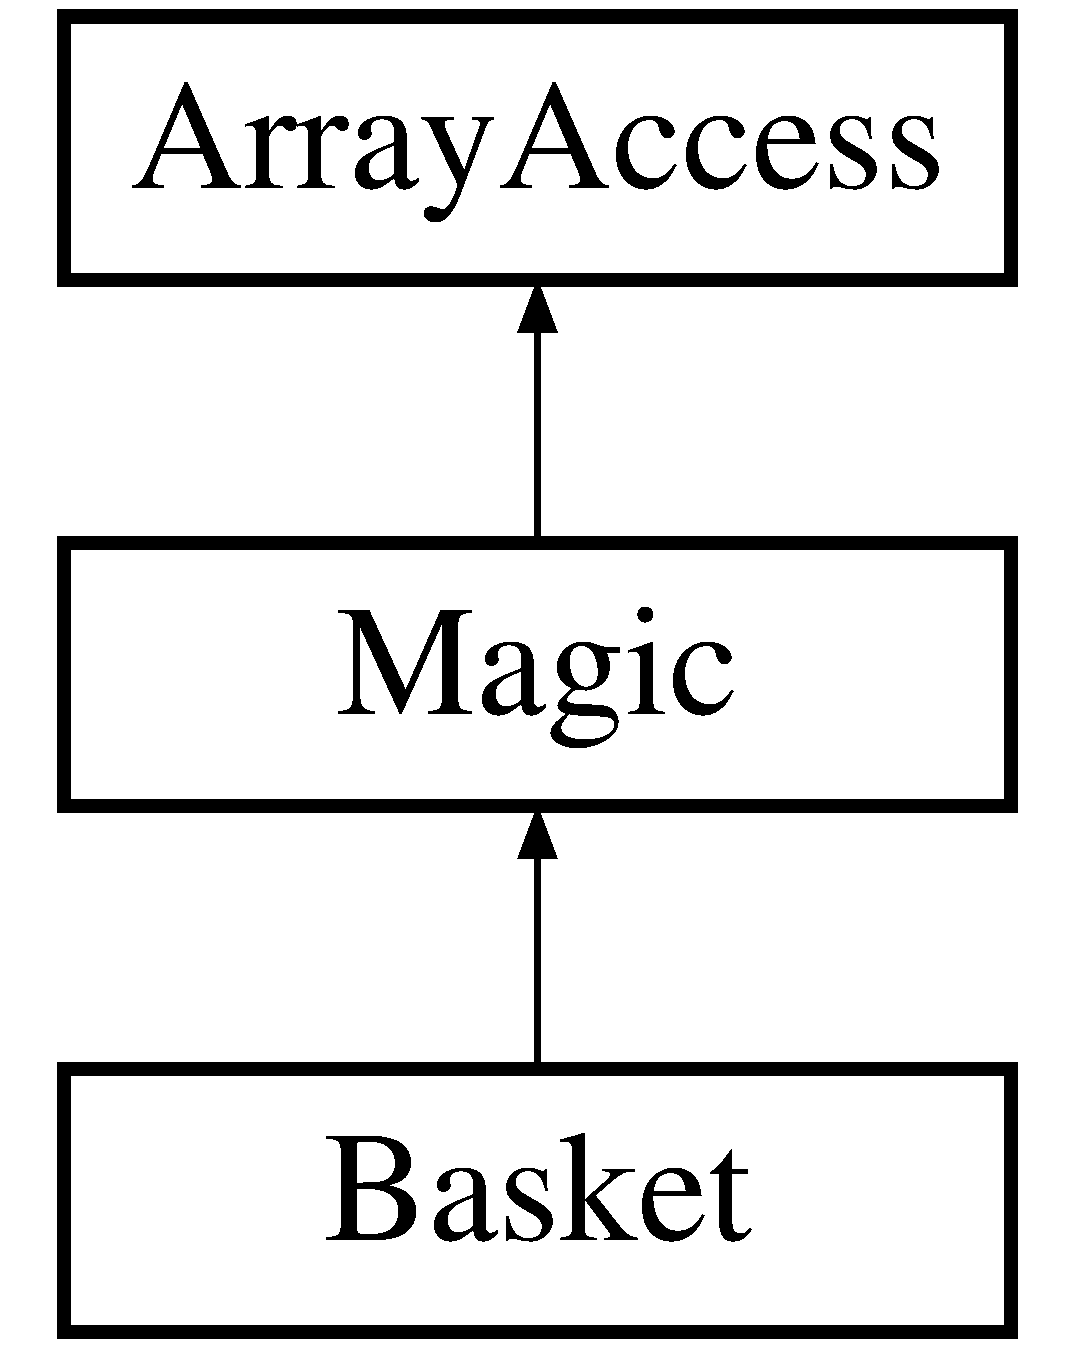
\includegraphics[height=3.000000cm]{class_basket}
\end{center}
\end{figure}
\subsection*{Public Member Functions}
\begin{DoxyCompactItemize}
\item 
\hyperlink{class_basket_ace1ae5be37bf26c172cc7ea4e1a65e26}{exists} (\$key)
\item 
\hyperlink{class_basket_ac8d8012023e560c81f55a629022cb65a}{set} (\$key, \$val)
\item 
\& \hyperlink{class_basket_ac3695923790b06917410e205068b8376}{get} (\$key)
\item 
\hyperlink{class_basket_a10a949ef75de6c82c98ac555f371ba83}{clear} (\$key)
\item 
\hyperlink{class_basket_ae24293a6c7fb1d109eb000b7f9db35c1}{find} (\$key=N\+U\+LL, \$val=N\+U\+LL)
\item 
\hyperlink{class_basket_ad9ce70d0a094124bff4adcec3df5e30f}{findone} (\$key, \$val)
\item 
\hyperlink{class_basket_abc7666f1c00ea27802ea7f19bdec2d17}{load} (\$key, \$val)
\item 
\hyperlink{class_basket_acc3a900450447c51540aaa9dec5959a4}{dry} ()
\item 
\hyperlink{class_basket_ac751e87b3d4c4bf2feb03bee8b092755}{count} ()
\item 
\hyperlink{class_basket_afc8a3c62679cf00ade9f15fb2a6d6132}{save} ()
\item 
\hyperlink{class_basket_ae25b1f24d58b7b7e6cd08fc07183fae5}{erase} (\$key, \$val)
\item 
\hyperlink{class_basket_a4a20559544fdf4dcb457e258dc976cf8}{reset} ()
\item 
\hyperlink{class_basket_aeb639e5b2b713ed87ab8f2033af98ae8}{drop} ()
\item 
\hyperlink{class_basket_a462833da5009a82b31e39d3b5db38abd}{copyfrom} (\$var)
\item 
\hyperlink{class_basket_a4bcf54f913758fb093c35ea81fc29615}{copyto} (\$key)
\item 
\hyperlink{class_basket_ac41b8e359a8eb81494e030062e7b4bad}{checkout} ()
\item 
\hyperlink{class_basket_ae34d667a85d03b5da0154d74ae414768}{\+\_\+\+\_\+construct} (\$key=\textquotesingle{}basket\textquotesingle{})
\end{DoxyCompactItemize}
\subsection*{Data Fields}
\begin{DoxyCompactItemize}
\item 
\hypertarget{class_basket_ae97941710d863131c700f069b109991e}{}\label{class_basket_ae97941710d863131c700f069b109991e} 
\hyperlink{class_basket_ae97941710d863131c700f069b109991e}{\$id}
\begin{DoxyCompactList}\small\item\em Current item identifier. \end{DoxyCompactList}\item 
\hypertarget{class_basket_aa61b415cee119a7511e05c405ecd0b32}{}\label{class_basket_aa61b415cee119a7511e05c405ecd0b32} 
\hyperlink{class_basket_aa61b415cee119a7511e05c405ecd0b32}{\$item} =\mbox{[}$\,$\mbox{]}
\begin{DoxyCompactList}\small\item\em Current item contents. \end{DoxyCompactList}\end{DoxyCompactItemize}
{\bf }\par
\begin{DoxyCompactItemize}
\item 
\hypertarget{class_basket_aa2e3f553fd1f1c2053bc084118c10396}{}\label{class_basket_aa2e3f553fd1f1c2053bc084118c10396} 
const {\bfseries E\+\_\+\+Field} =\textquotesingle{}Undefined field \%s\textquotesingle{}
\end{DoxyCompactItemize}

\subsection*{Protected Attributes}
\begin{DoxyCompactItemize}
\item 
\hypertarget{class_basket_aa60b0284e0dfa2463495481cf11e3cf4}{}\label{class_basket_aa60b0284e0dfa2463495481cf11e3cf4} 
\hyperlink{class_basket_aa60b0284e0dfa2463495481cf11e3cf4}{\$key}
\begin{DoxyCompactList}\small\item\em \hyperlink{class_session}{Session} key. \end{DoxyCompactList}\end{DoxyCompactItemize}


\subsection{Detailed Description}
Session-\/based pseudo-\/mapper. 

Definition at line 24 of file basket.\+php.



\subsection{Constructor \& Destructor Documentation}
\hypertarget{class_basket_ae34d667a85d03b5da0154d74ae414768}{}\label{class_basket_ae34d667a85d03b5da0154d74ae414768} 
\index{Basket@{Basket}!\+\_\+\+\_\+construct@{\+\_\+\+\_\+construct}}
\index{\+\_\+\+\_\+construct@{\+\_\+\+\_\+construct}!Basket@{Basket}}
\subsubsection{\texorpdfstring{\+\_\+\+\_\+construct()}{\_\_construct()}}
{\footnotesize\ttfamily \+\_\+\+\_\+construct (\begin{DoxyParamCaption}\item[{}]{\$key = {\ttfamily \textquotesingle{}basket\textquotesingle{}} }\end{DoxyParamCaption})}

Instantiate class \begin{DoxyReturn}{Returns}
void 
\end{DoxyReturn}

\begin{DoxyParams}{Parameters}
{\em \$key} & string \\
\hline
\end{DoxyParams}


Definition at line 230 of file basket.\+php.



\subsection{Member Function Documentation}
\hypertarget{class_basket_ac41b8e359a8eb81494e030062e7b4bad}{}\label{class_basket_ac41b8e359a8eb81494e030062e7b4bad} 
\index{Basket@{Basket}!checkout@{checkout}}
\index{checkout@{checkout}!Basket@{Basket}}
\subsubsection{\texorpdfstring{checkout()}{checkout()}}
{\footnotesize\ttfamily checkout (\begin{DoxyParamCaption}{ }\end{DoxyParamCaption})}

Check out basket contents \begin{DoxyReturn}{Returns}
array 
\end{DoxyReturn}


Definition at line 216 of file basket.\+php.

\hypertarget{class_basket_a10a949ef75de6c82c98ac555f371ba83}{}\label{class_basket_a10a949ef75de6c82c98ac555f371ba83} 
\index{Basket@{Basket}!clear@{clear}}
\index{clear@{clear}!Basket@{Basket}}
\subsubsection{\texorpdfstring{clear()}{clear()}}
{\footnotesize\ttfamily clear (\begin{DoxyParamCaption}\item[{}]{\$key }\end{DoxyParamCaption})}

Delete field \begin{DoxyReturn}{Returns}
N\+U\+LL 
\end{DoxyReturn}

\begin{DoxyParams}{Parameters}
{\em \$key} & string \\
\hline
\end{DoxyParams}


Definition at line 77 of file basket.\+php.

\hypertarget{class_basket_a462833da5009a82b31e39d3b5db38abd}{}\label{class_basket_a462833da5009a82b31e39d3b5db38abd} 
\index{Basket@{Basket}!copyfrom@{copyfrom}}
\index{copyfrom@{copyfrom}!Basket@{Basket}}
\subsubsection{\texorpdfstring{copyfrom()}{copyfrom()}}
{\footnotesize\ttfamily copyfrom (\begin{DoxyParamCaption}\item[{}]{\$var }\end{DoxyParamCaption})}

Hydrate item using hive array variable \begin{DoxyReturn}{Returns}
N\+U\+LL 
\end{DoxyReturn}

\begin{DoxyParams}{Parameters}
{\em \$var} & array$\vert$string \\
\hline
\end{DoxyParams}


Definition at line 194 of file basket.\+php.

\hypertarget{class_basket_a4bcf54f913758fb093c35ea81fc29615}{}\label{class_basket_a4bcf54f913758fb093c35ea81fc29615} 
\index{Basket@{Basket}!copyto@{copyto}}
\index{copyto@{copyto}!Basket@{Basket}}
\subsubsection{\texorpdfstring{copyto()}{copyto()}}
{\footnotesize\ttfamily copyto (\begin{DoxyParamCaption}\item[{}]{\$key }\end{DoxyParamCaption})}

Populate hive array variable with item contents \begin{DoxyReturn}{Returns}
N\+U\+LL 
\end{DoxyReturn}

\begin{DoxyParams}{Parameters}
{\em \$key} & string \\
\hline
\end{DoxyParams}


Definition at line 206 of file basket.\+php.

\hypertarget{class_basket_ac751e87b3d4c4bf2feb03bee8b092755}{}\label{class_basket_ac751e87b3d4c4bf2feb03bee8b092755} 
\index{Basket@{Basket}!count@{count}}
\index{count@{count}!Basket@{Basket}}
\subsubsection{\texorpdfstring{count()}{count()}}
{\footnotesize\ttfamily count (\begin{DoxyParamCaption}{ }\end{DoxyParamCaption})}

Return number of items in basket \begin{DoxyReturn}{Returns}
int 
\end{DoxyReturn}


Definition at line 140 of file basket.\+php.

\hypertarget{class_basket_aeb639e5b2b713ed87ab8f2033af98ae8}{}\label{class_basket_aeb639e5b2b713ed87ab8f2033af98ae8} 
\index{Basket@{Basket}!drop@{drop}}
\index{drop@{drop}!Basket@{Basket}}
\subsubsection{\texorpdfstring{drop()}{drop()}}
{\footnotesize\ttfamily drop (\begin{DoxyParamCaption}{ }\end{DoxyParamCaption})}

Empty basket \begin{DoxyReturn}{Returns}
N\+U\+LL 
\end{DoxyReturn}


Definition at line 185 of file basket.\+php.

\hypertarget{class_basket_acc3a900450447c51540aaa9dec5959a4}{}\label{class_basket_acc3a900450447c51540aaa9dec5959a4} 
\index{Basket@{Basket}!dry@{dry}}
\index{dry@{dry}!Basket@{Basket}}
\subsubsection{\texorpdfstring{dry()}{dry()}}
{\footnotesize\ttfamily dry (\begin{DoxyParamCaption}{ }\end{DoxyParamCaption})}

Return T\+R\+UE if current item is empty/undefined \begin{DoxyReturn}{Returns}
bool 
\end{DoxyReturn}


Definition at line 132 of file basket.\+php.

\hypertarget{class_basket_ae25b1f24d58b7b7e6cd08fc07183fae5}{}\label{class_basket_ae25b1f24d58b7b7e6cd08fc07183fae5} 
\index{Basket@{Basket}!erase@{erase}}
\index{erase@{erase}!Basket@{Basket}}
\subsubsection{\texorpdfstring{erase()}{erase()}}
{\footnotesize\ttfamily erase (\begin{DoxyParamCaption}\item[{}]{\$key,  }\item[{}]{\$val }\end{DoxyParamCaption})}

Erase item matching key/value pair \begin{DoxyReturn}{Returns}
bool 
\end{DoxyReturn}

\begin{DoxyParams}{Parameters}
{\em \$key} & string \\
\hline
{\em \$val} & mixed \\
\hline
\end{DoxyParams}


Definition at line 161 of file basket.\+php.

\hypertarget{class_basket_ace1ae5be37bf26c172cc7ea4e1a65e26}{}\label{class_basket_ace1ae5be37bf26c172cc7ea4e1a65e26} 
\index{Basket@{Basket}!exists@{exists}}
\index{exists@{exists}!Basket@{Basket}}
\subsubsection{\texorpdfstring{exists()}{exists()}}
{\footnotesize\ttfamily exists (\begin{DoxyParamCaption}\item[{}]{\$key }\end{DoxyParamCaption})}

Return T\+R\+UE if field is defined \begin{DoxyReturn}{Returns}
bool 
\end{DoxyReturn}

\begin{DoxyParams}{Parameters}
{\em \$key} & string \\
\hline
\end{DoxyParams}


Definition at line 44 of file basket.\+php.

\hypertarget{class_basket_ae24293a6c7fb1d109eb000b7f9db35c1}{}\label{class_basket_ae24293a6c7fb1d109eb000b7f9db35c1} 
\index{Basket@{Basket}!find@{find}}
\index{find@{find}!Basket@{Basket}}
\subsubsection{\texorpdfstring{find()}{find()}}
{\footnotesize\ttfamily find (\begin{DoxyParamCaption}\item[{}]{\$key = {\ttfamily NULL},  }\item[{}]{\$val = {\ttfamily NULL} }\end{DoxyParamCaption})}

Return items that match key/value pair; If no key/value pair specified, return all items \begin{DoxyReturn}{Returns}
array 
\end{DoxyReturn}

\begin{DoxyParams}{Parameters}
{\em \$key} & string \\
\hline
{\em \$val} & mixed \\
\hline
\end{DoxyParams}


Definition at line 88 of file basket.\+php.

\hypertarget{class_basket_ad9ce70d0a094124bff4adcec3df5e30f}{}\label{class_basket_ad9ce70d0a094124bff4adcec3df5e30f} 
\index{Basket@{Basket}!findone@{findone}}
\index{findone@{findone}!Basket@{Basket}}
\subsubsection{\texorpdfstring{findone()}{findone()}}
{\footnotesize\ttfamily findone (\begin{DoxyParamCaption}\item[{}]{\$key,  }\item[{}]{\$val }\end{DoxyParamCaption})}

Return first item that matches key/value pair \begin{DoxyReturn}{Returns}
object$\vert$\+F\+A\+L\+SE 
\end{DoxyReturn}

\begin{DoxyParams}{Parameters}
{\em \$key} & string \\
\hline
{\em \$val} & mixed \\
\hline
\end{DoxyParams}


Definition at line 109 of file basket.\+php.

\hypertarget{class_basket_ac3695923790b06917410e205068b8376}{}\label{class_basket_ac3695923790b06917410e205068b8376} 
\index{Basket@{Basket}!get@{get}}
\index{get@{get}!Basket@{Basket}}
\subsubsection{\texorpdfstring{get()}{get()}}
{\footnotesize\ttfamily \& get (\begin{DoxyParamCaption}\item[{}]{\$key }\end{DoxyParamCaption})}

Retrieve value of field \begin{DoxyReturn}{Returns}
scalar$\vert$\+F\+A\+L\+SE 
\end{DoxyReturn}

\begin{DoxyParams}{Parameters}
{\em \$key} & string \\
\hline
\end{DoxyParams}


Definition at line 63 of file basket.\+php.

\hypertarget{class_basket_abc7666f1c00ea27802ea7f19bdec2d17}{}\label{class_basket_abc7666f1c00ea27802ea7f19bdec2d17} 
\index{Basket@{Basket}!load@{load}}
\index{load@{load}!Basket@{Basket}}
\subsubsection{\texorpdfstring{load()}{load()}}
{\footnotesize\ttfamily load (\begin{DoxyParamCaption}\item[{}]{\$key,  }\item[{}]{\$val }\end{DoxyParamCaption})}

Map current item to matching key/value pair \begin{DoxyReturn}{Returns}
array 
\end{DoxyReturn}

\begin{DoxyParams}{Parameters}
{\em \$key} & string \\
\hline
{\em \$val} & mixed \\
\hline
\end{DoxyParams}


Definition at line 119 of file basket.\+php.

\hypertarget{class_basket_a4a20559544fdf4dcb457e258dc976cf8}{}\label{class_basket_a4a20559544fdf4dcb457e258dc976cf8} 
\index{Basket@{Basket}!reset@{reset}}
\index{reset@{reset}!Basket@{Basket}}
\subsubsection{\texorpdfstring{reset()}{reset()}}
{\footnotesize\ttfamily reset (\begin{DoxyParamCaption}{ }\end{DoxyParamCaption})}

Reset cursor \begin{DoxyReturn}{Returns}
N\+U\+LL 
\end{DoxyReturn}


Definition at line 176 of file basket.\+php.

\hypertarget{class_basket_afc8a3c62679cf00ade9f15fb2a6d6132}{}\label{class_basket_afc8a3c62679cf00ade9f15fb2a6d6132} 
\index{Basket@{Basket}!save@{save}}
\index{save@{save}!Basket@{Basket}}
\subsubsection{\texorpdfstring{save()}{save()}}
{\footnotesize\ttfamily save (\begin{DoxyParamCaption}{ }\end{DoxyParamCaption})}

Save current item \begin{DoxyReturn}{Returns}
array 
\end{DoxyReturn}


Definition at line 148 of file basket.\+php.

\hypertarget{class_basket_ac8d8012023e560c81f55a629022cb65a}{}\label{class_basket_ac8d8012023e560c81f55a629022cb65a} 
\index{Basket@{Basket}!set@{set}}
\index{set@{set}!Basket@{Basket}}
\subsubsection{\texorpdfstring{set()}{set()}}
{\footnotesize\ttfamily set (\begin{DoxyParamCaption}\item[{}]{\$key,  }\item[{}]{\$val }\end{DoxyParamCaption})}

Assign value to field \begin{DoxyReturn}{Returns}
scalar$\vert$\+F\+A\+L\+SE 
\end{DoxyReturn}

\begin{DoxyParams}{Parameters}
{\em \$key} & string \\
\hline
{\em \$val} & scalar \\
\hline
\end{DoxyParams}


Definition at line 54 of file basket.\+php.



The documentation for this class was generated from the following file\+:\begin{DoxyCompactItemize}
\item 
/\+Users/aplennevaux/\+G\+I\+T\+H\+U\+B/\+Visionary-\/website/src/vendor/bcosca/fatfree/lib/basket.\+php\end{DoxyCompactItemize}

\hypertarget{class_bcrypt}{}\section{Bcrypt Class Reference}
\label{class_bcrypt}\index{Bcrypt@{Bcrypt}}
Inheritance diagram for Bcrypt\+:\begin{figure}[H]
\begin{center}
\leavevmode
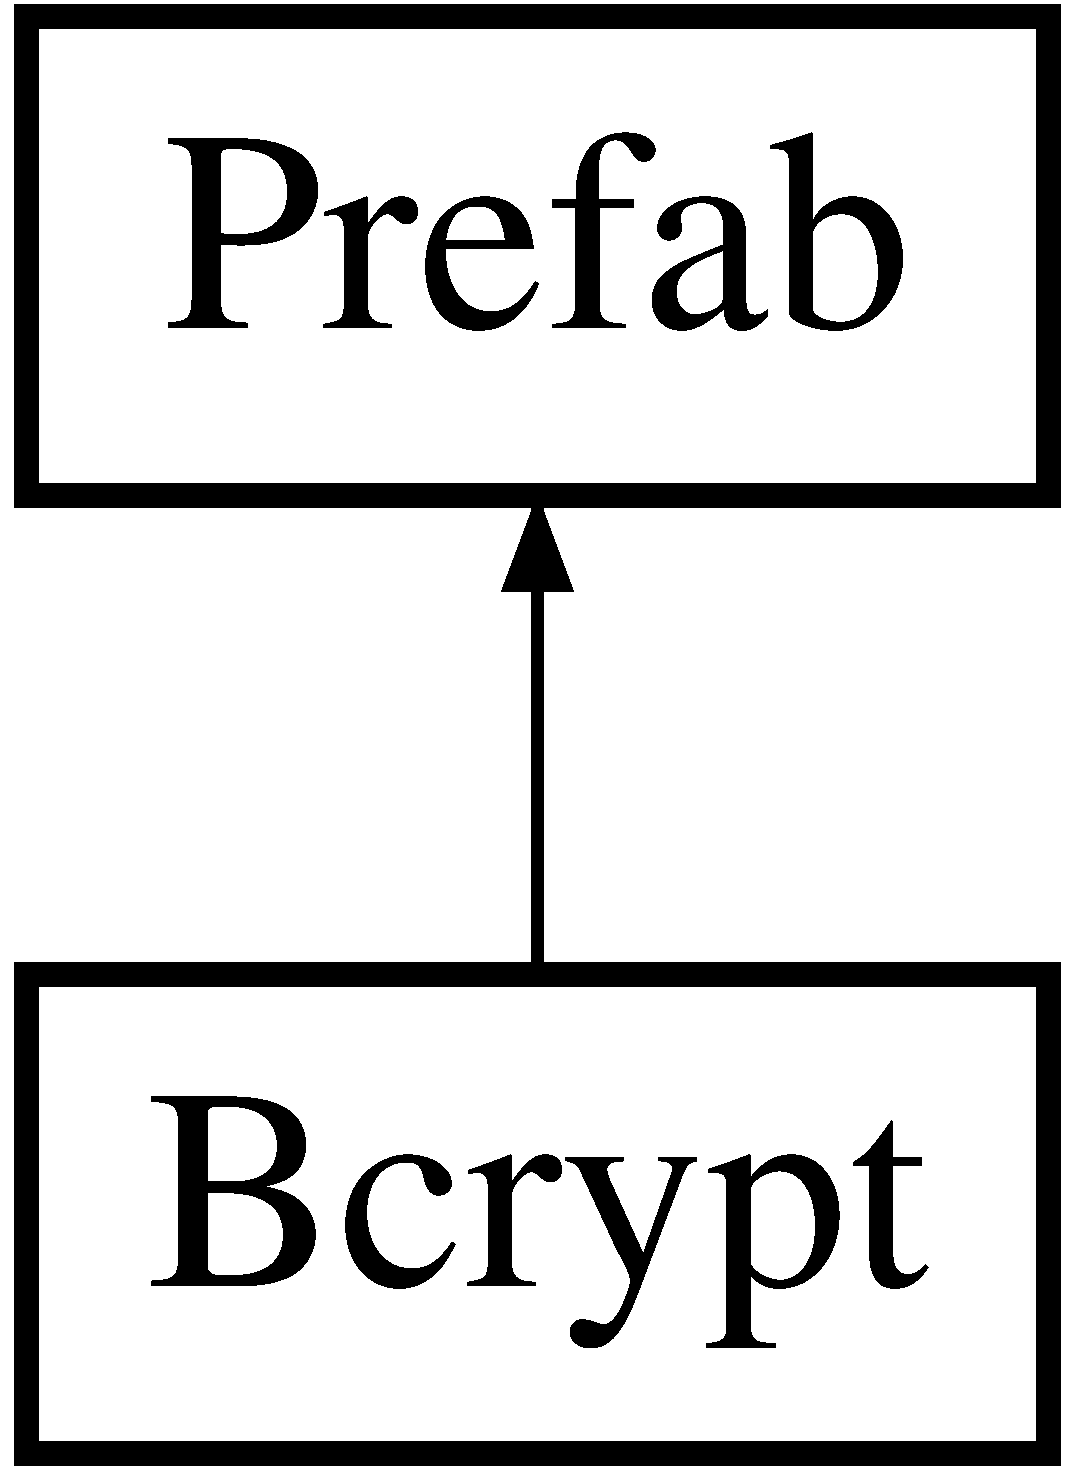
\includegraphics[height=2.000000cm]{class_bcrypt}
\end{center}
\end{figure}
\subsection*{Public Member Functions}
\begin{DoxyCompactItemize}
\item 
\hyperlink{class_bcrypt_a027c5d961c1d96ac0fa2a0fcc4af1e71}{hash} (\$pw, \$salt=N\+U\+LL, \$cost=self\+::\+C\+O\+ST)
\item 
\hyperlink{class_bcrypt_a426e49c6c92d63e97240374a30e44989}{needs\+\_\+rehash} (\$\hyperlink{class_bcrypt_a027c5d961c1d96ac0fa2a0fcc4af1e71}{hash}, \$cost=self\+::\+C\+O\+ST)
\item 
\hyperlink{class_bcrypt_a88aa522c359b8f4adff496b507df9864}{verify} (\$pw, \$\hyperlink{class_bcrypt_a027c5d961c1d96ac0fa2a0fcc4af1e71}{hash})
\end{DoxyCompactItemize}
\subsection*{Data Fields}
\begin{DoxyCompactItemize}
\item 
\hypertarget{class_bcrypt_a086e0e15867645a7a8cf461bf8ce1e0c}{}\label{class_bcrypt_a086e0e15867645a7a8cf461bf8ce1e0c} 
const \hyperlink{class_bcrypt_a086e0e15867645a7a8cf461bf8ce1e0c}{C\+O\+ST} =10
\begin{DoxyCompactList}\small\item\em Default cost. \end{DoxyCompactList}\end{DoxyCompactItemize}
{\bf }\par
\begin{DoxyCompactItemize}
\item 
\hypertarget{class_bcrypt_a8713f533d972d7d3f0637941061f9b8a}{}\label{class_bcrypt_a8713f533d972d7d3f0637941061f9b8a} 
const {\bfseries E\+\_\+\+Cost\+Arg} =\textquotesingle{}Invalid cost parameter\textquotesingle{}
\item 
\hypertarget{class_bcrypt_aaea1f538f70ff2c05db136dd0fe74db4}{}\label{class_bcrypt_aaea1f538f70ff2c05db136dd0fe74db4} 
const {\bfseries E\+\_\+\+Salt\+Arg} =\textquotesingle{}Salt must be at least 22 alphanumeric characters\textquotesingle{}
\end{DoxyCompactItemize}

\subsection*{Additional Inherited Members}


\subsection{Detailed Description}
Lightweight password hashing library

Copyright (c) 2009-\/2016 F3\+::\+Factory/\+Bong Cosca, All rights reserved.

This file is part of the Fat-\/\+Free Framework (\href{http://fatfreeframework.com}{\tt http\+://fatfreeframework.\+com}).

This is free software\+: you can redistribute it and/or modify it under the terms of the G\+NU General Public License as published by the Free Software Foundation, either version 3 of the License, or later.

Fat-\/\+Free Framework is distributed in the hope that it will be useful, but W\+I\+T\+H\+O\+UT A\+NY W\+A\+R\+R\+A\+N\+TY; without even the implied warranty of M\+E\+R\+C\+H\+A\+N\+T\+A\+B\+I\+L\+I\+TY or F\+I\+T\+N\+E\+SS F\+OR A P\+A\+R\+T\+I\+C\+U\+L\+AR P\+U\+R\+P\+O\+SE. See the G\+NU General Public License for more details.

You should have received a copy of the G\+NU General Public License along with Fat-\/\+Free Framework. If not, see \href{http://www.gnu.org/licenses/}{\tt http\+://www.\+gnu.\+org/licenses/}.

\begin{DoxyRefDesc}{Deprecated}
\item[\hyperlink{deprecated__deprecated000001}{Deprecated}]use \href{http://php.net/manual/en/ref.password.php}{\tt http\+://php.\+net/manual/en/ref.\+password.\+php} instead (P\+HP 5.\+5+ only) \end{DoxyRefDesc}


Definition at line 25 of file bcrypt.\+php.



\subsection{Member Function Documentation}
\hypertarget{class_bcrypt_a027c5d961c1d96ac0fa2a0fcc4af1e71}{}\label{class_bcrypt_a027c5d961c1d96ac0fa2a0fcc4af1e71} 
\index{Bcrypt@{Bcrypt}!hash@{hash}}
\index{hash@{hash}!Bcrypt@{Bcrypt}}
\subsubsection{\texorpdfstring{hash()}{hash()}}
{\footnotesize\ttfamily hash (\begin{DoxyParamCaption}\item[{}]{\$pw,  }\item[{}]{\$salt = {\ttfamily NULL},  }\item[{}]{\$cost = {\ttfamily self\+:\+:COST} }\end{DoxyParamCaption})}

Generate bcrypt hash of string \begin{DoxyReturn}{Returns}
string$\vert$\+F\+A\+L\+SE 
\end{DoxyReturn}

\begin{DoxyParams}{Parameters}
{\em \$pw} & string \\
\hline
{\em \$salt} & string \\
\hline
{\em \$cost} & int \\
\hline
\end{DoxyParams}


Definition at line 44 of file bcrypt.\+php.

\hypertarget{class_bcrypt_a426e49c6c92d63e97240374a30e44989}{}\label{class_bcrypt_a426e49c6c92d63e97240374a30e44989} 
\index{Bcrypt@{Bcrypt}!needs\+\_\+rehash@{needs\+\_\+rehash}}
\index{needs\+\_\+rehash@{needs\+\_\+rehash}!Bcrypt@{Bcrypt}}
\subsubsection{\texorpdfstring{needs\+\_\+rehash()}{needs\_rehash()}}
{\footnotesize\ttfamily needs\+\_\+rehash (\begin{DoxyParamCaption}\item[{}]{\$hash,  }\item[{}]{\$cost = {\ttfamily self\+:\+:COST} }\end{DoxyParamCaption})}

Check if password is still strong enough \begin{DoxyReturn}{Returns}
bool 
\end{DoxyReturn}

\begin{DoxyParams}{Parameters}
{\em \$hash} & string \\
\hline
{\em \$cost} & int \\
\hline
\end{DoxyParams}


Definition at line 75 of file bcrypt.\+php.

\hypertarget{class_bcrypt_a88aa522c359b8f4adff496b507df9864}{}\label{class_bcrypt_a88aa522c359b8f4adff496b507df9864} 
\index{Bcrypt@{Bcrypt}!verify@{verify}}
\index{verify@{verify}!Bcrypt@{Bcrypt}}
\subsubsection{\texorpdfstring{verify()}{verify()}}
{\footnotesize\ttfamily verify (\begin{DoxyParamCaption}\item[{}]{\$pw,  }\item[{}]{\$hash }\end{DoxyParamCaption})}

Verify password against hash using timing attack resistant approach \begin{DoxyReturn}{Returns}
bool 
\end{DoxyReturn}

\begin{DoxyParams}{Parameters}
{\em \$pw} & string \\
\hline
{\em \$hash} & string \\
\hline
\end{DoxyParams}


Definition at line 86 of file bcrypt.\+php.



The documentation for this class was generated from the following file\+:\begin{DoxyCompactItemize}
\item 
/\+Users/aplennevaux/\+G\+I\+T\+H\+U\+B/\+Visionary-\/website/src/vendor/bcosca/fatfree/lib/bcrypt.\+php\end{DoxyCompactItemize}

\hypertarget{class_cache}{}\section{Cache Class Reference}
\label{class_cache}\index{Cache@{Cache}}


\hyperlink{class_cache}{Cache} engine.  


Inheritance diagram for Cache\+:\begin{figure}[H]
\begin{center}
\leavevmode
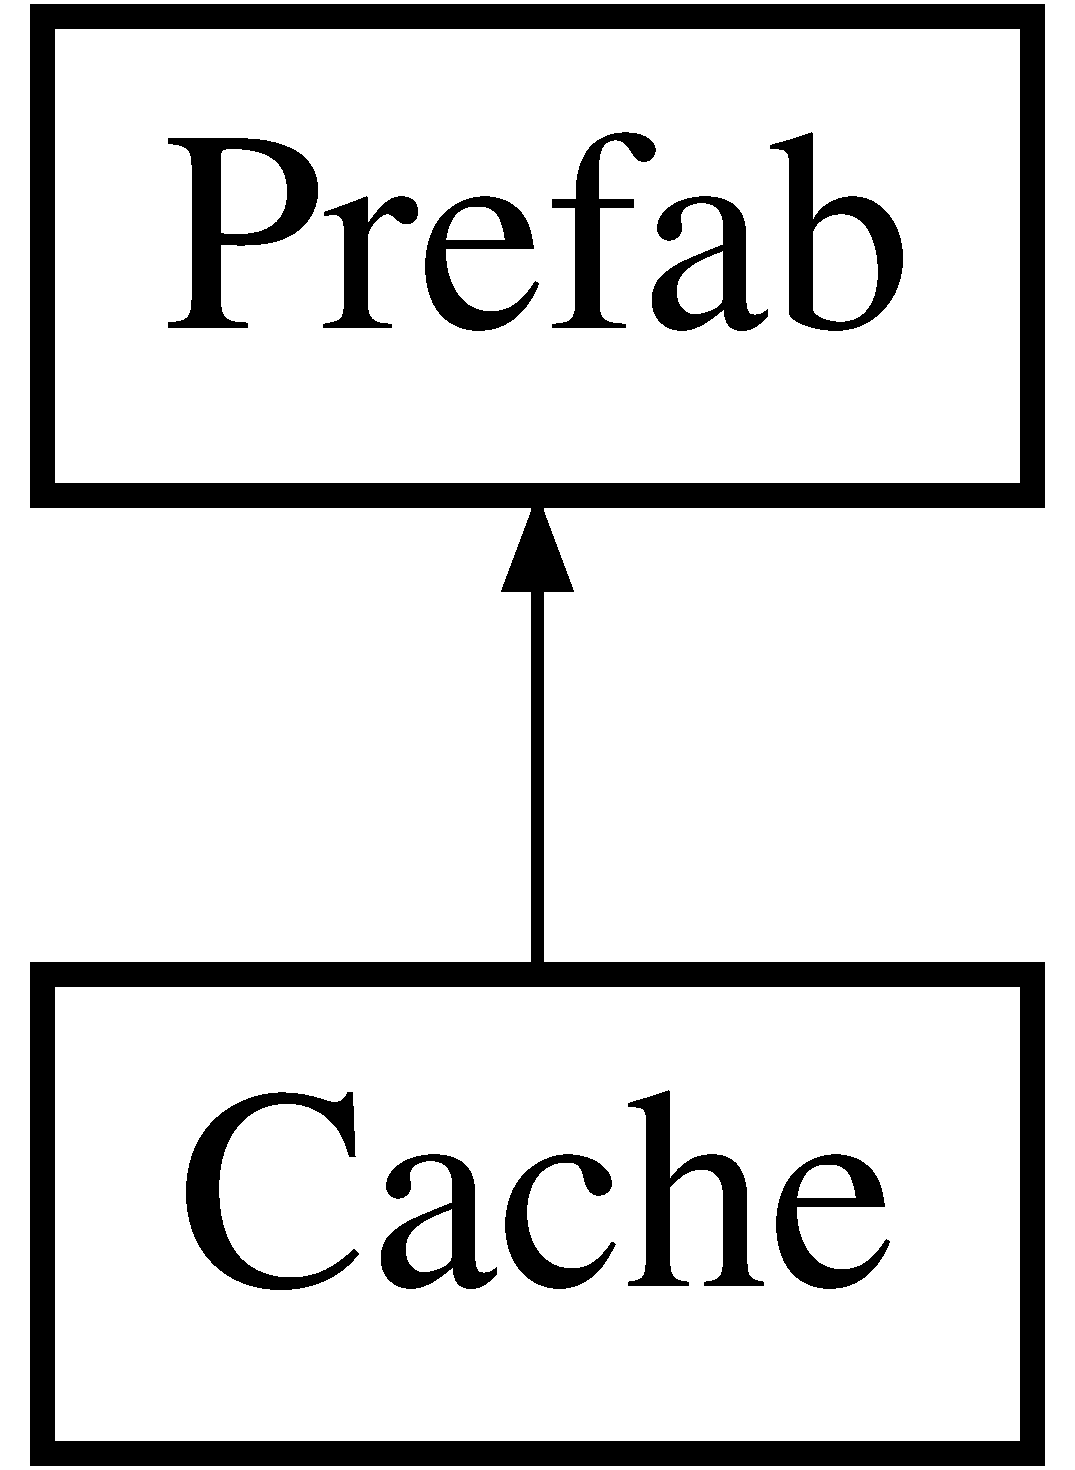
\includegraphics[height=2.000000cm]{class_cache}
\end{center}
\end{figure}
\subsection*{Public Member Functions}
\begin{DoxyCompactItemize}
\item 
\hyperlink{class_cache_a28497caad131119319e31168c38713b6}{exists} (\$key, \&\$val=N\+U\+LL)
\item 
\hyperlink{class_cache_a845297666b2c78affb9fa78605ebf93e}{set} (\$key, \$val, \$ttl=0)
\item 
\hyperlink{class_cache_a24a9bf83a1002d46ece83a93d14bd921}{get} (\$key)
\item 
\hyperlink{class_cache_a10a949ef75de6c82c98ac555f371ba83}{clear} (\$key)
\item 
\hyperlink{class_cache_ada19e349da5d9093164fe0c05b1d5bf3}{reset} (\$suffix=N\+U\+LL, \$lifetime=0)
\item 
\hyperlink{class_cache_a0c573a775b081079b350498980565fa2}{load} (\$dsn)
\item 
\hyperlink{class_cache_a53b443dea5ef4422f7335a380e654c98}{\+\_\+\+\_\+construct} (\$dsn=F\+A\+L\+SE)
\end{DoxyCompactItemize}
\subsection*{Data Fields}
\begin{DoxyCompactItemize}
\item 
\hypertarget{class_cache_a09e8cf95b9d29955a0bfabca9b420edc}{}\label{class_cache_a09e8cf95b9d29955a0bfabca9b420edc} 
\hyperlink{class_cache_a09e8cf95b9d29955a0bfabca9b420edc}{\$prefix}
\begin{DoxyCompactList}\small\item\em Prefix for cache entries. \end{DoxyCompactList}\item 
\hypertarget{class_cache_af63b439d0c69c1a6e9c2d1b9a4f4af9e}{}\label{class_cache_af63b439d0c69c1a6e9c2d1b9a4f4af9e} 
\hyperlink{class_cache_af63b439d0c69c1a6e9c2d1b9a4f4af9e}{\$ref}
\begin{DoxyCompactList}\small\item\em Mem\+Cache or Redis object. \end{DoxyCompactList}\end{DoxyCompactItemize}
\subsection*{Protected Attributes}
\begin{DoxyCompactItemize}
\item 
\hypertarget{class_cache_a6441cca8c9fa11e16d2017e8cb733c10}{}\label{class_cache_a6441cca8c9fa11e16d2017e8cb733c10} 
\hyperlink{class_cache_a6441cca8c9fa11e16d2017e8cb733c10}{\$dsn}
\begin{DoxyCompactList}\small\item\em \hyperlink{class_cache}{Cache} D\+SN. \end{DoxyCompactList}\end{DoxyCompactItemize}
\subsection*{Additional Inherited Members}


\subsection{Detailed Description}
\hyperlink{class_cache}{Cache} engine. 

Definition at line 2345 of file base.\+php.



\subsection{Constructor \& Destructor Documentation}
\hypertarget{class_cache_a53b443dea5ef4422f7335a380e654c98}{}\label{class_cache_a53b443dea5ef4422f7335a380e654c98} 
\index{Cache@{Cache}!\+\_\+\+\_\+construct@{\+\_\+\+\_\+construct}}
\index{\+\_\+\+\_\+construct@{\+\_\+\+\_\+construct}!Cache@{Cache}}
\subsubsection{\texorpdfstring{\+\_\+\+\_\+construct()}{\_\_construct()}}
{\footnotesize\ttfamily \+\_\+\+\_\+construct (\begin{DoxyParamCaption}\item[{}]{\$dsn = {\ttfamily FALSE} }\end{DoxyParamCaption})}

Class constructor \begin{DoxyReturn}{Returns}
object 
\end{DoxyReturn}

\begin{DoxyParams}{Parameters}
{\em \$dsn} & bool$\vert$string \\
\hline
\end{DoxyParams}


Definition at line 2588 of file base.\+php.



\subsection{Member Function Documentation}
\hypertarget{class_cache_a10a949ef75de6c82c98ac555f371ba83}{}\label{class_cache_a10a949ef75de6c82c98ac555f371ba83} 
\index{Cache@{Cache}!clear@{clear}}
\index{clear@{clear}!Cache@{Cache}}
\subsubsection{\texorpdfstring{clear()}{clear()}}
{\footnotesize\ttfamily clear (\begin{DoxyParamCaption}\item[{}]{\$key }\end{DoxyParamCaption})}

Delete cache entry \begin{DoxyReturn}{Returns}
bool 
\end{DoxyReturn}

\begin{DoxyParams}{Parameters}
{\em \$key} & string \\
\hline
\end{DoxyParams}


Definition at line 2447 of file base.\+php.

\hypertarget{class_cache_a28497caad131119319e31168c38713b6}{}\label{class_cache_a28497caad131119319e31168c38713b6} 
\index{Cache@{Cache}!exists@{exists}}
\index{exists@{exists}!Cache@{Cache}}
\subsubsection{\texorpdfstring{exists()}{exists()}}
{\footnotesize\ttfamily exists (\begin{DoxyParamCaption}\item[{}]{\$key,  }\item[{\&}]{\$val = {\ttfamily NULL} }\end{DoxyParamCaption})}

Return timestamp and T\+TL of cache entry or F\+A\+L\+SE if not found \begin{DoxyReturn}{Returns}
array$\vert$\+F\+A\+L\+SE 
\end{DoxyReturn}

\begin{DoxyParams}{Parameters}
{\em \$key} & string \\
\hline
{\em \$val} & mixed \\
\hline
\end{DoxyParams}


Definition at line 2361 of file base.\+php.

\hypertarget{class_cache_a24a9bf83a1002d46ece83a93d14bd921}{}\label{class_cache_a24a9bf83a1002d46ece83a93d14bd921} 
\index{Cache@{Cache}!get@{get}}
\index{get@{get}!Cache@{Cache}}
\subsubsection{\texorpdfstring{get()}{get()}}
{\footnotesize\ttfamily get (\begin{DoxyParamCaption}\item[{}]{\$key }\end{DoxyParamCaption})}

Retrieve value of cache entry \begin{DoxyReturn}{Returns}
mixed$\vert$\+F\+A\+L\+SE 
\end{DoxyReturn}

\begin{DoxyParams}{Parameters}
{\em \$key} & string \\
\hline
\end{DoxyParams}


Definition at line 2438 of file base.\+php.

\hypertarget{class_cache_a0c573a775b081079b350498980565fa2}{}\label{class_cache_a0c573a775b081079b350498980565fa2} 
\index{Cache@{Cache}!load@{load}}
\index{load@{load}!Cache@{Cache}}
\subsubsection{\texorpdfstring{load()}{load()}}
{\footnotesize\ttfamily load (\begin{DoxyParamCaption}\item[{}]{\$dsn }\end{DoxyParamCaption})}

Load/auto-\/detect cache backend \begin{DoxyReturn}{Returns}
string 
\end{DoxyReturn}

\begin{DoxyParams}{Parameters}
{\em \$dsn} & bool$\vert$string \\
\hline
\end{DoxyParams}


Definition at line 2547 of file base.\+php.

\hypertarget{class_cache_ada19e349da5d9093164fe0c05b1d5bf3}{}\label{class_cache_ada19e349da5d9093164fe0c05b1d5bf3} 
\index{Cache@{Cache}!reset@{reset}}
\index{reset@{reset}!Cache@{Cache}}
\subsubsection{\texorpdfstring{reset()}{reset()}}
{\footnotesize\ttfamily reset (\begin{DoxyParamCaption}\item[{}]{\$suffix = {\ttfamily NULL},  }\item[{}]{\$lifetime = {\ttfamily 0} }\end{DoxyParamCaption})}

Clear contents of cache backend \begin{DoxyReturn}{Returns}
bool 
\end{DoxyReturn}

\begin{DoxyParams}{Parameters}
{\em \$suffix} & string \\
\hline
{\em \$lifetime} & int \\
\hline
\end{DoxyParams}


Definition at line 2476 of file base.\+php.

\hypertarget{class_cache_a845297666b2c78affb9fa78605ebf93e}{}\label{class_cache_a845297666b2c78affb9fa78605ebf93e} 
\index{Cache@{Cache}!set@{set}}
\index{set@{set}!Cache@{Cache}}
\subsubsection{\texorpdfstring{set()}{set()}}
{\footnotesize\ttfamily set (\begin{DoxyParamCaption}\item[{}]{\$key,  }\item[{}]{\$val,  }\item[{}]{\$ttl = {\ttfamily 0} }\end{DoxyParamCaption})}

Store value in cache \begin{DoxyReturn}{Returns}
mixed$\vert$\+F\+A\+L\+SE 
\end{DoxyReturn}

\begin{DoxyParams}{Parameters}
{\em \$key} & string \\
\hline
{\em \$val} & mixed \\
\hline
{\em \$ttl} & int \\
\hline
\end{DoxyParams}


Definition at line 2405 of file base.\+php.



The documentation for this class was generated from the following file\+:\begin{DoxyCompactItemize}
\item 
/\+Users/aplennevaux/\+G\+I\+T\+H\+U\+B/\+Visionary-\/website/src/vendor/bcosca/fatfree/lib/base.\+php\end{DoxyCompactItemize}

\hypertarget{class_d_b_1_1_cursor}{}\section{Cursor Class Reference}
\label{class_d_b_1_1_cursor}\index{Cursor@{Cursor}}


Simple cursor implementation.  


Inheritance diagram for Cursor\+:\begin{figure}[H]
\begin{center}
\leavevmode
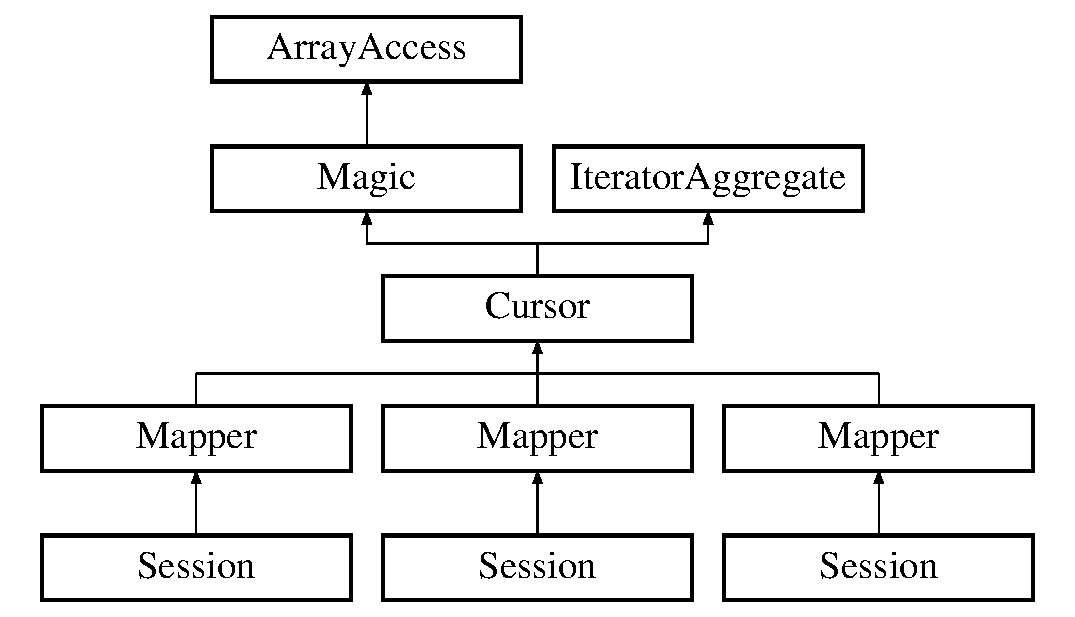
\includegraphics[height=5.000000cm]{class_d_b_1_1_cursor}
\end{center}
\end{figure}
\subsection*{Public Member Functions}
\begin{DoxyCompactItemize}
\item 
\hyperlink{class_d_b_1_1_cursor_a38948c2fb1711f49b72f123cbd91e611}{dbtype} ()
\item 
\hyperlink{class_d_b_1_1_cursor_a9dfc1601eaf8348bed6ba5622f725971}{fields} ()
\item 
\hyperlink{class_d_b_1_1_cursor_aa33294a722f17e6e4946223bb73f13ab}{cast} (\$obj=N\+U\+LL)
\item 
\hyperlink{class_d_b_1_1_cursor_a45e70f55799839fc0286bc94000924a7}{find} (\$filter=N\+U\+LL, array \$options=N\+U\+LL, \$ttl=0)
\item 
\hyperlink{class_d_b_1_1_cursor_ab1f3a3bd85dca49dceaea57f2fe21abf}{count} (\$filter=N\+U\+LL, \$ttl=0)
\item 
\hyperlink{class_d_b_1_1_cursor_a473241246338cfccc4709ba896749019}{insert} ()
\item 
\hyperlink{class_d_b_1_1_cursor_a842e4774e3b3601a005b995c02f7e883}{update} ()
\item 
\hyperlink{class_d_b_1_1_cursor_adffe904ab38af888d9b033647ec6d935}{copyfrom} (\$var, \$func=N\+U\+LL)
\item 
\hyperlink{class_d_b_1_1_cursor_a4bcf54f913758fb093c35ea81fc29615}{copyto} (\$key)
\item 
\hyperlink{class_d_b_1_1_cursor_a7f835c25df4cb49d02328644722656da}{getiterator} ()
\item 
\hyperlink{class_d_b_1_1_cursor_acc3a900450447c51540aaa9dec5959a4}{dry} ()
\item 
\hyperlink{class_d_b_1_1_cursor_abf73a1aa82ad1233b41388c0a4711c86}{findone} (\$filter=N\+U\+LL, array \$options=N\+U\+LL, \$ttl=0)
\item 
\hyperlink{class_d_b_1_1_cursor_a51889c022407cdc6cc565afa5ffe2715}{paginate} ( \$pos=0, \$size=10, \$filter=N\+U\+LL, array \$options=N\+U\+LL, \$ttl=0)
\item 
\hyperlink{class_d_b_1_1_cursor_a4db66c122e6274a3d653eff639e8476f}{load} (\$filter=N\+U\+LL, array \$options=N\+U\+LL, \$ttl=0)
\item 
\hyperlink{class_d_b_1_1_cursor_a3f07a4aa73e71d525744db933bc2aff4}{loaded} ()
\item 
\hyperlink{class_d_b_1_1_cursor_ac73eef9ff76ea330c0dab36ca448b90d}{first} ()
\item 
\hyperlink{class_d_b_1_1_cursor_ac90cadb327363232bb2d83a4f8ebd613}{last} ()
\item 
\hyperlink{class_d_b_1_1_cursor_aad399d205074eaeed711d5e0157b3c0a}{skip} (\$ofs=1)
\item 
\hyperlink{class_d_b_1_1_cursor_acea62048bfee7b3cd80ed446c86fb78a}{next} ()
\item 
\hyperlink{class_d_b_1_1_cursor_a190535b88008d474b610585a5d9eb84c}{prev} ()
\item 
\hyperlink{class_d_b_1_1_cursor_abb9f0d6adf1eb9b3b55712056861a247}{valid} ()
\item 
\hyperlink{class_d_b_1_1_cursor_afc8a3c62679cf00ade9f15fb2a6d6132}{save} ()
\item 
\hyperlink{class_d_b_1_1_cursor_a933f3fa1037c8b797bdd237d811edf82}{erase} ()
\item 
\hyperlink{class_d_b_1_1_cursor_a7615e052068ed5e2c78a87f9b562f98e}{onload} (\$func)
\item 
\hyperlink{class_d_b_1_1_cursor_ae34d64fef3b7e4de2eede65ca67751d7}{beforeinsert} (\$func)
\item 
\hyperlink{class_d_b_1_1_cursor_a192a31bc101b9aafb4e1300883d33dc6}{afterinsert} (\$func)
\item 
\hyperlink{class_d_b_1_1_cursor_ab3ebd70359a4d0916e07bc3523099fff}{oninsert} (\$func)
\item 
\hyperlink{class_d_b_1_1_cursor_a9f11326bbf4cdec47ac4f1d143f1dfba}{beforeupdate} (\$func)
\item 
\hyperlink{class_d_b_1_1_cursor_a2b621278d4f2ed751338a1d1bfb60e70}{afterupdate} (\$func)
\item 
\hyperlink{class_d_b_1_1_cursor_a6af536a479e72aff418c5965eff20320}{onupdate} (\$func)
\item 
\hyperlink{class_d_b_1_1_cursor_a9d837ab7aea1a740986d5f6c0258b395}{beforesave} (\$func)
\item 
\hyperlink{class_d_b_1_1_cursor_a4b19070ae7f1fc2edeee8e0252f8ebb2}{aftersave} (\$func)
\item 
\hyperlink{class_d_b_1_1_cursor_a507f285ea3bb622446f79e07e838e147}{onsave} (\$func)
\item 
\hyperlink{class_d_b_1_1_cursor_a50acd223a47511be7b2e92dd1d504268}{beforeerase} (\$func)
\item 
\hyperlink{class_d_b_1_1_cursor_aa8c748ed4bf2cba7c84ce360e00dbe2a}{aftererase} (\$func)
\item 
\hyperlink{class_d_b_1_1_cursor_aebef85c8e2c1ece8cb36a60dc332595f}{onerase} (\$func)
\item 
\hyperlink{class_d_b_1_1_cursor_a4a20559544fdf4dcb457e258dc976cf8}{reset} ()
\end{DoxyCompactItemize}
\subsection*{Data Fields}
\begin{DoxyCompactItemize}
\item 
\hypertarget{class_d_b_1_1_cursor_a18682bea3799d50bb3a0cc3d049dca07}{}\label{class_d_b_1_1_cursor_a18682bea3799d50bb3a0cc3d049dca07} 
\hyperlink{class_d_b_1_1_cursor_a18682bea3799d50bb3a0cc3d049dca07}{\$ptr} =0
\begin{DoxyCompactList}\small\item\em Current position. \end{DoxyCompactList}\item 
\hypertarget{class_d_b_1_1_cursor_ae4c540bb943eedf48dbc7d06b2994a05}{}\label{class_d_b_1_1_cursor_ae4c540bb943eedf48dbc7d06b2994a05} 
\hyperlink{class_d_b_1_1_cursor_ae4c540bb943eedf48dbc7d06b2994a05}{\$trigger} =\mbox{[}$\,$\mbox{]}
\begin{DoxyCompactList}\small\item\em Event listeners. \end{DoxyCompactList}\end{DoxyCompactItemize}
{\bf }\par
\begin{DoxyCompactItemize}
\item 
\hypertarget{class_d_b_1_1_cursor_aa2e3f553fd1f1c2053bc084118c10396}{}\label{class_d_b_1_1_cursor_aa2e3f553fd1f1c2053bc084118c10396} 
const {\bfseries E\+\_\+\+Field} =\textquotesingle{}Undefined field \%s\textquotesingle{}
\end{DoxyCompactItemize}

\subsection*{Protected Attributes}
\begin{DoxyCompactItemize}
\item 
\hypertarget{class_d_b_1_1_cursor_af59a5f7cd609e592c41dc3643efd3c98}{}\label{class_d_b_1_1_cursor_af59a5f7cd609e592c41dc3643efd3c98} 
\hyperlink{class_d_b_1_1_cursor_af59a5f7cd609e592c41dc3643efd3c98}{\$query} =\mbox{[}$\,$\mbox{]}
\begin{DoxyCompactList}\small\item\em Query results. \end{DoxyCompactList}\end{DoxyCompactItemize}


\subsection{Detailed Description}
Simple cursor implementation. 

Definition at line 26 of file cursor.\+php.



\subsection{Member Function Documentation}
\hypertarget{class_d_b_1_1_cursor_aa8c748ed4bf2cba7c84ce360e00dbe2a}{}\label{class_d_b_1_1_cursor_aa8c748ed4bf2cba7c84ce360e00dbe2a} 
\index{D\+B\+::\+Cursor@{D\+B\+::\+Cursor}!aftererase@{aftererase}}
\index{aftererase@{aftererase}!D\+B\+::\+Cursor@{D\+B\+::\+Cursor}}
\subsubsection{\texorpdfstring{aftererase()}{aftererase()}}
{\footnotesize\ttfamily aftererase (\begin{DoxyParamCaption}\item[{}]{\$func }\end{DoxyParamCaption})}

Define aftererase trigger \begin{DoxyReturn}{Returns}
callback 
\end{DoxyReturn}

\begin{DoxyParams}{Parameters}
{\em \$func} & callback \\
\hline
\end{DoxyParams}


Definition at line 363 of file cursor.\+php.

\hypertarget{class_d_b_1_1_cursor_a192a31bc101b9aafb4e1300883d33dc6}{}\label{class_d_b_1_1_cursor_a192a31bc101b9aafb4e1300883d33dc6} 
\index{D\+B\+::\+Cursor@{D\+B\+::\+Cursor}!afterinsert@{afterinsert}}
\index{afterinsert@{afterinsert}!D\+B\+::\+Cursor@{D\+B\+::\+Cursor}}
\subsubsection{\texorpdfstring{afterinsert()}{afterinsert()}}
{\footnotesize\ttfamily afterinsert (\begin{DoxyParamCaption}\item[{}]{\$func }\end{DoxyParamCaption})}

Define afterinsert trigger \begin{DoxyReturn}{Returns}
callback 
\end{DoxyReturn}

\begin{DoxyParams}{Parameters}
{\em \$func} & callback \\
\hline
\end{DoxyParams}


Definition at line 278 of file cursor.\+php.

\hypertarget{class_d_b_1_1_cursor_a4b19070ae7f1fc2edeee8e0252f8ebb2}{}\label{class_d_b_1_1_cursor_a4b19070ae7f1fc2edeee8e0252f8ebb2} 
\index{D\+B\+::\+Cursor@{D\+B\+::\+Cursor}!aftersave@{aftersave}}
\index{aftersave@{aftersave}!D\+B\+::\+Cursor@{D\+B\+::\+Cursor}}
\subsubsection{\texorpdfstring{aftersave()}{aftersave()}}
{\footnotesize\ttfamily aftersave (\begin{DoxyParamCaption}\item[{}]{\$func }\end{DoxyParamCaption})}

Define aftersave trigger \begin{DoxyReturn}{Returns}
callback 
\end{DoxyReturn}

\begin{DoxyParams}{Parameters}
{\em \$func} & callback \\
\hline
\end{DoxyParams}


Definition at line 334 of file cursor.\+php.

\hypertarget{class_d_b_1_1_cursor_a2b621278d4f2ed751338a1d1bfb60e70}{}\label{class_d_b_1_1_cursor_a2b621278d4f2ed751338a1d1bfb60e70} 
\index{D\+B\+::\+Cursor@{D\+B\+::\+Cursor}!afterupdate@{afterupdate}}
\index{afterupdate@{afterupdate}!D\+B\+::\+Cursor@{D\+B\+::\+Cursor}}
\subsubsection{\texorpdfstring{afterupdate()}{afterupdate()}}
{\footnotesize\ttfamily afterupdate (\begin{DoxyParamCaption}\item[{}]{\$func }\end{DoxyParamCaption})}

Define afterupdate trigger \begin{DoxyReturn}{Returns}
callback 
\end{DoxyReturn}

\begin{DoxyParams}{Parameters}
{\em \$func} & callback \\
\hline
\end{DoxyParams}


Definition at line 305 of file cursor.\+php.

\hypertarget{class_d_b_1_1_cursor_a50acd223a47511be7b2e92dd1d504268}{}\label{class_d_b_1_1_cursor_a50acd223a47511be7b2e92dd1d504268} 
\index{D\+B\+::\+Cursor@{D\+B\+::\+Cursor}!beforeerase@{beforeerase}}
\index{beforeerase@{beforeerase}!D\+B\+::\+Cursor@{D\+B\+::\+Cursor}}
\subsubsection{\texorpdfstring{beforeerase()}{beforeerase()}}
{\footnotesize\ttfamily beforeerase (\begin{DoxyParamCaption}\item[{}]{\$func }\end{DoxyParamCaption})}

Define beforeerase trigger \begin{DoxyReturn}{Returns}
callback 
\end{DoxyReturn}

\begin{DoxyParams}{Parameters}
{\em \$func} & callback \\
\hline
\end{DoxyParams}


Definition at line 354 of file cursor.\+php.

\hypertarget{class_d_b_1_1_cursor_ae34d64fef3b7e4de2eede65ca67751d7}{}\label{class_d_b_1_1_cursor_ae34d64fef3b7e4de2eede65ca67751d7} 
\index{D\+B\+::\+Cursor@{D\+B\+::\+Cursor}!beforeinsert@{beforeinsert}}
\index{beforeinsert@{beforeinsert}!D\+B\+::\+Cursor@{D\+B\+::\+Cursor}}
\subsubsection{\texorpdfstring{beforeinsert()}{beforeinsert()}}
{\footnotesize\ttfamily beforeinsert (\begin{DoxyParamCaption}\item[{}]{\$func }\end{DoxyParamCaption})}

Define beforeinsert trigger \begin{DoxyReturn}{Returns}
callback 
\end{DoxyReturn}

\begin{DoxyParams}{Parameters}
{\em \$func} & callback \\
\hline
\end{DoxyParams}


Definition at line 269 of file cursor.\+php.

\hypertarget{class_d_b_1_1_cursor_a9d837ab7aea1a740986d5f6c0258b395}{}\label{class_d_b_1_1_cursor_a9d837ab7aea1a740986d5f6c0258b395} 
\index{D\+B\+::\+Cursor@{D\+B\+::\+Cursor}!beforesave@{beforesave}}
\index{beforesave@{beforesave}!D\+B\+::\+Cursor@{D\+B\+::\+Cursor}}
\subsubsection{\texorpdfstring{beforesave()}{beforesave()}}
{\footnotesize\ttfamily beforesave (\begin{DoxyParamCaption}\item[{}]{\$func }\end{DoxyParamCaption})}

Define beforesave trigger \begin{DoxyReturn}{Returns}
callback 
\end{DoxyReturn}

\begin{DoxyParams}{Parameters}
{\em \$func} & callback \\
\hline
\end{DoxyParams}


Definition at line 323 of file cursor.\+php.

\hypertarget{class_d_b_1_1_cursor_a9f11326bbf4cdec47ac4f1d143f1dfba}{}\label{class_d_b_1_1_cursor_a9f11326bbf4cdec47ac4f1d143f1dfba} 
\index{D\+B\+::\+Cursor@{D\+B\+::\+Cursor}!beforeupdate@{beforeupdate}}
\index{beforeupdate@{beforeupdate}!D\+B\+::\+Cursor@{D\+B\+::\+Cursor}}
\subsubsection{\texorpdfstring{beforeupdate()}{beforeupdate()}}
{\footnotesize\ttfamily beforeupdate (\begin{DoxyParamCaption}\item[{}]{\$func }\end{DoxyParamCaption})}

Define beforeupdate trigger \begin{DoxyReturn}{Returns}
callback 
\end{DoxyReturn}

\begin{DoxyParams}{Parameters}
{\em \$func} & callback \\
\hline
\end{DoxyParams}


Definition at line 296 of file cursor.\+php.

\hypertarget{class_d_b_1_1_cursor_aa33294a722f17e6e4946223bb73f13ab}{}\label{class_d_b_1_1_cursor_aa33294a722f17e6e4946223bb73f13ab} 
\index{D\+B\+::\+Cursor@{D\+B\+::\+Cursor}!cast@{cast}}
\index{cast@{cast}!D\+B\+::\+Cursor@{D\+B\+::\+Cursor}}
\subsubsection{\texorpdfstring{cast()}{cast()}}
{\footnotesize\ttfamily cast (\begin{DoxyParamCaption}\item[{}]{\$obj = {\ttfamily NULL} }\end{DoxyParamCaption})\hspace{0.3cm}{\ttfamily [abstract]}}

Return fields of mapper object as an associative array \begin{DoxyReturn}{Returns}
array 
\end{DoxyReturn}

\begin{DoxyParams}{Parameters}
{\em \$obj} & object \\
\hline
\end{DoxyParams}
\hypertarget{class_d_b_1_1_cursor_adffe904ab38af888d9b033647ec6d935}{}\label{class_d_b_1_1_cursor_adffe904ab38af888d9b033647ec6d935} 
\index{D\+B\+::\+Cursor@{D\+B\+::\+Cursor}!copyfrom@{copyfrom}}
\index{copyfrom@{copyfrom}!D\+B\+::\+Cursor@{D\+B\+::\+Cursor}}
\subsubsection{\texorpdfstring{copyfrom()}{copyfrom()}}
{\footnotesize\ttfamily copyfrom (\begin{DoxyParamCaption}\item[{}]{\$var,  }\item[{}]{\$func = {\ttfamily NULL} }\end{DoxyParamCaption})\hspace{0.3cm}{\ttfamily [abstract]}}

Hydrate mapper object using hive array variable \begin{DoxyReturn}{Returns}
N\+U\+LL 
\end{DoxyReturn}

\begin{DoxyParams}{Parameters}
{\em \$var} & array$\vert$string \\
\hline
{\em \$func} & callback \\
\hline
\end{DoxyParams}
\hypertarget{class_d_b_1_1_cursor_a4bcf54f913758fb093c35ea81fc29615}{}\label{class_d_b_1_1_cursor_a4bcf54f913758fb093c35ea81fc29615} 
\index{D\+B\+::\+Cursor@{D\+B\+::\+Cursor}!copyto@{copyto}}
\index{copyto@{copyto}!D\+B\+::\+Cursor@{D\+B\+::\+Cursor}}
\subsubsection{\texorpdfstring{copyto()}{copyto()}}
{\footnotesize\ttfamily copyto (\begin{DoxyParamCaption}\item[{}]{\$key }\end{DoxyParamCaption})\hspace{0.3cm}{\ttfamily [abstract]}}

Populate hive array variable with mapper fields \begin{DoxyReturn}{Returns}
N\+U\+LL 
\end{DoxyReturn}

\begin{DoxyParams}{Parameters}
{\em \$key} & string \\
\hline
\end{DoxyParams}
\hypertarget{class_d_b_1_1_cursor_ab1f3a3bd85dca49dceaea57f2fe21abf}{}\label{class_d_b_1_1_cursor_ab1f3a3bd85dca49dceaea57f2fe21abf} 
\index{D\+B\+::\+Cursor@{D\+B\+::\+Cursor}!count@{count}}
\index{count@{count}!D\+B\+::\+Cursor@{D\+B\+::\+Cursor}}
\subsubsection{\texorpdfstring{count()}{count()}}
{\footnotesize\ttfamily count (\begin{DoxyParamCaption}\item[{}]{\$filter = {\ttfamily NULL},  }\item[{}]{\$ttl = {\ttfamily 0} }\end{DoxyParamCaption})\hspace{0.3cm}{\ttfamily [abstract]}}

Count records that match criteria \begin{DoxyReturn}{Returns}
int 
\end{DoxyReturn}

\begin{DoxyParams}{Parameters}
{\em \$filter} & array \\
\hline
{\em \$ttl} & int \\
\hline
\end{DoxyParams}
\hypertarget{class_d_b_1_1_cursor_a38948c2fb1711f49b72f123cbd91e611}{}\label{class_d_b_1_1_cursor_a38948c2fb1711f49b72f123cbd91e611} 
\index{D\+B\+::\+Cursor@{D\+B\+::\+Cursor}!dbtype@{dbtype}}
\index{dbtype@{dbtype}!D\+B\+::\+Cursor@{D\+B\+::\+Cursor}}
\subsubsection{\texorpdfstring{dbtype()}{dbtype()}}
{\footnotesize\ttfamily dbtype (\begin{DoxyParamCaption}{ }\end{DoxyParamCaption})\hspace{0.3cm}{\ttfamily [abstract]}}

Return database type \begin{DoxyReturn}{Returns}
string 
\end{DoxyReturn}
\hypertarget{class_d_b_1_1_cursor_acc3a900450447c51540aaa9dec5959a4}{}\label{class_d_b_1_1_cursor_acc3a900450447c51540aaa9dec5959a4} 
\index{D\+B\+::\+Cursor@{D\+B\+::\+Cursor}!dry@{dry}}
\index{dry@{dry}!D\+B\+::\+Cursor@{D\+B\+::\+Cursor}}
\subsubsection{\texorpdfstring{dry()}{dry()}}
{\footnotesize\ttfamily dry (\begin{DoxyParamCaption}{ }\end{DoxyParamCaption})}

Return T\+R\+UE if current cursor position is not mapped to any record \begin{DoxyReturn}{Returns}
bool 
\end{DoxyReturn}


Definition at line 116 of file cursor.\+php.

\hypertarget{class_d_b_1_1_cursor_a933f3fa1037c8b797bdd237d811edf82}{}\label{class_d_b_1_1_cursor_a933f3fa1037c8b797bdd237d811edf82} 
\index{D\+B\+::\+Cursor@{D\+B\+::\+Cursor}!erase@{erase}}
\index{erase@{erase}!D\+B\+::\+Cursor@{D\+B\+::\+Cursor}}
\subsubsection{\texorpdfstring{erase()}{erase()}}
{\footnotesize\ttfamily erase (\begin{DoxyParamCaption}{ }\end{DoxyParamCaption})}

Delete current record \begin{DoxyReturn}{Returns}
int$\vert$bool 
\end{DoxyReturn}


Definition at line 249 of file cursor.\+php.

\hypertarget{class_d_b_1_1_cursor_a9dfc1601eaf8348bed6ba5622f725971}{}\label{class_d_b_1_1_cursor_a9dfc1601eaf8348bed6ba5622f725971} 
\index{D\+B\+::\+Cursor@{D\+B\+::\+Cursor}!fields@{fields}}
\index{fields@{fields}!D\+B\+::\+Cursor@{D\+B\+::\+Cursor}}
\subsubsection{\texorpdfstring{fields()}{fields()}}
{\footnotesize\ttfamily fields (\begin{DoxyParamCaption}{ }\end{DoxyParamCaption})\hspace{0.3cm}{\ttfamily [abstract]}}

Return field names \begin{DoxyReturn}{Returns}
array 
\end{DoxyReturn}
\hypertarget{class_d_b_1_1_cursor_a45e70f55799839fc0286bc94000924a7}{}\label{class_d_b_1_1_cursor_a45e70f55799839fc0286bc94000924a7} 
\index{D\+B\+::\+Cursor@{D\+B\+::\+Cursor}!find@{find}}
\index{find@{find}!D\+B\+::\+Cursor@{D\+B\+::\+Cursor}}
\subsubsection{\texorpdfstring{find()}{find()}}
{\footnotesize\ttfamily find (\begin{DoxyParamCaption}\item[{}]{\$filter = {\ttfamily NULL},  }\item[{array}]{\$options = {\ttfamily NULL},  }\item[{}]{\$ttl = {\ttfamily 0} }\end{DoxyParamCaption})\hspace{0.3cm}{\ttfamily [abstract]}}

Return records (array of mapper objects) that match criteria \begin{DoxyReturn}{Returns}
array 
\end{DoxyReturn}

\begin{DoxyParams}{Parameters}
{\em \$filter} & string$\vert$array \\
\hline
{\em \$options} & array \\
\hline
{\em \$ttl} & int \\
\hline
\end{DoxyParams}
\hypertarget{class_d_b_1_1_cursor_abf73a1aa82ad1233b41388c0a4711c86}{}\label{class_d_b_1_1_cursor_abf73a1aa82ad1233b41388c0a4711c86} 
\index{D\+B\+::\+Cursor@{D\+B\+::\+Cursor}!findone@{findone}}
\index{findone@{findone}!D\+B\+::\+Cursor@{D\+B\+::\+Cursor}}
\subsubsection{\texorpdfstring{findone()}{findone()}}
{\footnotesize\ttfamily findone (\begin{DoxyParamCaption}\item[{}]{\$filter = {\ttfamily NULL},  }\item[{array}]{\$options = {\ttfamily NULL},  }\item[{}]{\$ttl = {\ttfamily 0} }\end{DoxyParamCaption})}

Return first record (mapper object) that matches criteria \begin{DoxyReturn}{Returns}
static$\vert$\+F\+A\+L\+SE 
\end{DoxyReturn}

\begin{DoxyParams}{Parameters}
{\em \$filter} & string$\vert$array \\
\hline
{\em \$options} & array \\
\hline
{\em \$ttl} & int \\
\hline
\end{DoxyParams}


Definition at line 127 of file cursor.\+php.

\hypertarget{class_d_b_1_1_cursor_ac73eef9ff76ea330c0dab36ca448b90d}{}\label{class_d_b_1_1_cursor_ac73eef9ff76ea330c0dab36ca448b90d} 
\index{D\+B\+::\+Cursor@{D\+B\+::\+Cursor}!first@{first}}
\index{first@{first}!D\+B\+::\+Cursor@{D\+B\+::\+Cursor}}
\subsubsection{\texorpdfstring{first()}{first()}}
{\footnotesize\ttfamily first (\begin{DoxyParamCaption}{ }\end{DoxyParamCaption})}

Map to first record in cursor \begin{DoxyReturn}{Returns}
mixed 
\end{DoxyReturn}


Definition at line 191 of file cursor.\+php.

\hypertarget{class_d_b_1_1_cursor_a7f835c25df4cb49d02328644722656da}{}\label{class_d_b_1_1_cursor_a7f835c25df4cb49d02328644722656da} 
\index{D\+B\+::\+Cursor@{D\+B\+::\+Cursor}!getiterator@{getiterator}}
\index{getiterator@{getiterator}!D\+B\+::\+Cursor@{D\+B\+::\+Cursor}}
\subsubsection{\texorpdfstring{getiterator()}{getiterator()}}
{\footnotesize\ttfamily getiterator (\begin{DoxyParamCaption}{ }\end{DoxyParamCaption})\hspace{0.3cm}{\ttfamily [abstract]}}

Get cursor\textquotesingle{}s equivalent external iterator Causes a fatal error in P\+HP 5.\+3.\+5 if uncommented return Array\+Iterator \hypertarget{class_d_b_1_1_cursor_a473241246338cfccc4709ba896749019}{}\label{class_d_b_1_1_cursor_a473241246338cfccc4709ba896749019} 
\index{D\+B\+::\+Cursor@{D\+B\+::\+Cursor}!insert@{insert}}
\index{insert@{insert}!D\+B\+::\+Cursor@{D\+B\+::\+Cursor}}
\subsubsection{\texorpdfstring{insert()}{insert()}}
{\footnotesize\ttfamily insert (\begin{DoxyParamCaption}{ }\end{DoxyParamCaption})\hspace{0.3cm}{\ttfamily [abstract]}}

Insert new record \begin{DoxyReturn}{Returns}
array 
\end{DoxyReturn}
\hypertarget{class_d_b_1_1_cursor_ac90cadb327363232bb2d83a4f8ebd613}{}\label{class_d_b_1_1_cursor_ac90cadb327363232bb2d83a4f8ebd613} 
\index{D\+B\+::\+Cursor@{D\+B\+::\+Cursor}!last@{last}}
\index{last@{last}!D\+B\+::\+Cursor@{D\+B\+::\+Cursor}}
\subsubsection{\texorpdfstring{last()}{last()}}
{\footnotesize\ttfamily last (\begin{DoxyParamCaption}{ }\end{DoxyParamCaption})}

Map to last record in cursor \begin{DoxyReturn}{Returns}
mixed 
\end{DoxyReturn}


Definition at line 199 of file cursor.\+php.

\hypertarget{class_d_b_1_1_cursor_a4db66c122e6274a3d653eff639e8476f}{}\label{class_d_b_1_1_cursor_a4db66c122e6274a3d653eff639e8476f} 
\index{D\+B\+::\+Cursor@{D\+B\+::\+Cursor}!load@{load}}
\index{load@{load}!D\+B\+::\+Cursor@{D\+B\+::\+Cursor}}
\subsubsection{\texorpdfstring{load()}{load()}}
{\footnotesize\ttfamily load (\begin{DoxyParamCaption}\item[{}]{\$filter = {\ttfamily NULL},  }\item[{array}]{\$options = {\ttfamily NULL},  }\item[{}]{\$ttl = {\ttfamily 0} }\end{DoxyParamCaption})}

Map to first record that matches criteria \begin{DoxyReturn}{Returns}
array$\vert$\+F\+A\+L\+SE 
\end{DoxyReturn}

\begin{DoxyParams}{Parameters}
{\em \$filter} & string$\vert$array \\
\hline
{\em \$options} & array \\
\hline
{\em \$ttl} & int \\
\hline
\end{DoxyParams}


Definition at line 173 of file cursor.\+php.

\hypertarget{class_d_b_1_1_cursor_a3f07a4aa73e71d525744db933bc2aff4}{}\label{class_d_b_1_1_cursor_a3f07a4aa73e71d525744db933bc2aff4} 
\index{D\+B\+::\+Cursor@{D\+B\+::\+Cursor}!loaded@{loaded}}
\index{loaded@{loaded}!D\+B\+::\+Cursor@{D\+B\+::\+Cursor}}
\subsubsection{\texorpdfstring{loaded()}{loaded()}}
{\footnotesize\ttfamily loaded (\begin{DoxyParamCaption}{ }\end{DoxyParamCaption})}

Return the count of records loaded \begin{DoxyReturn}{Returns}
int 
\end{DoxyReturn}


Definition at line 183 of file cursor.\+php.

\hypertarget{class_d_b_1_1_cursor_acea62048bfee7b3cd80ed446c86fb78a}{}\label{class_d_b_1_1_cursor_acea62048bfee7b3cd80ed446c86fb78a} 
\index{D\+B\+::\+Cursor@{D\+B\+::\+Cursor}!next@{next}}
\index{next@{next}!D\+B\+::\+Cursor@{D\+B\+::\+Cursor}}
\subsubsection{\texorpdfstring{next()}{next()}}
{\footnotesize\ttfamily next (\begin{DoxyParamCaption}{ }\end{DoxyParamCaption})}

Map next record \begin{DoxyReturn}{Returns}
mixed 
\end{DoxyReturn}


Definition at line 218 of file cursor.\+php.

\hypertarget{class_d_b_1_1_cursor_aebef85c8e2c1ece8cb36a60dc332595f}{}\label{class_d_b_1_1_cursor_aebef85c8e2c1ece8cb36a60dc332595f} 
\index{D\+B\+::\+Cursor@{D\+B\+::\+Cursor}!onerase@{onerase}}
\index{onerase@{onerase}!D\+B\+::\+Cursor@{D\+B\+::\+Cursor}}
\subsubsection{\texorpdfstring{onerase()}{onerase()}}
{\footnotesize\ttfamily onerase (\begin{DoxyParamCaption}\item[{}]{\$func }\end{DoxyParamCaption})}

Define onerase trigger \begin{DoxyReturn}{Returns}
callback 
\end{DoxyReturn}

\begin{DoxyParams}{Parameters}
{\em \$func} & callback \\
\hline
\end{DoxyParams}


Definition at line 372 of file cursor.\+php.

\hypertarget{class_d_b_1_1_cursor_ab3ebd70359a4d0916e07bc3523099fff}{}\label{class_d_b_1_1_cursor_ab3ebd70359a4d0916e07bc3523099fff} 
\index{D\+B\+::\+Cursor@{D\+B\+::\+Cursor}!oninsert@{oninsert}}
\index{oninsert@{oninsert}!D\+B\+::\+Cursor@{D\+B\+::\+Cursor}}
\subsubsection{\texorpdfstring{oninsert()}{oninsert()}}
{\footnotesize\ttfamily oninsert (\begin{DoxyParamCaption}\item[{}]{\$func }\end{DoxyParamCaption})}

Define oninsert trigger \begin{DoxyReturn}{Returns}
callback 
\end{DoxyReturn}

\begin{DoxyParams}{Parameters}
{\em \$func} & callback \\
\hline
\end{DoxyParams}


Definition at line 287 of file cursor.\+php.

\hypertarget{class_d_b_1_1_cursor_a7615e052068ed5e2c78a87f9b562f98e}{}\label{class_d_b_1_1_cursor_a7615e052068ed5e2c78a87f9b562f98e} 
\index{D\+B\+::\+Cursor@{D\+B\+::\+Cursor}!onload@{onload}}
\index{onload@{onload}!D\+B\+::\+Cursor@{D\+B\+::\+Cursor}}
\subsubsection{\texorpdfstring{onload()}{onload()}}
{\footnotesize\ttfamily onload (\begin{DoxyParamCaption}\item[{}]{\$func }\end{DoxyParamCaption})}

Define onload trigger \begin{DoxyReturn}{Returns}
callback 
\end{DoxyReturn}

\begin{DoxyParams}{Parameters}
{\em \$func} & callback \\
\hline
\end{DoxyParams}


Definition at line 260 of file cursor.\+php.

\hypertarget{class_d_b_1_1_cursor_a507f285ea3bb622446f79e07e838e147}{}\label{class_d_b_1_1_cursor_a507f285ea3bb622446f79e07e838e147} 
\index{D\+B\+::\+Cursor@{D\+B\+::\+Cursor}!onsave@{onsave}}
\index{onsave@{onsave}!D\+B\+::\+Cursor@{D\+B\+::\+Cursor}}
\subsubsection{\texorpdfstring{onsave()}{onsave()}}
{\footnotesize\ttfamily onsave (\begin{DoxyParamCaption}\item[{}]{\$func }\end{DoxyParamCaption})}

Define onsave trigger \begin{DoxyReturn}{Returns}
callback 
\end{DoxyReturn}

\begin{DoxyParams}{Parameters}
{\em \$func} & callback \\
\hline
\end{DoxyParams}


Definition at line 345 of file cursor.\+php.

\hypertarget{class_d_b_1_1_cursor_a6af536a479e72aff418c5965eff20320}{}\label{class_d_b_1_1_cursor_a6af536a479e72aff418c5965eff20320} 
\index{D\+B\+::\+Cursor@{D\+B\+::\+Cursor}!onupdate@{onupdate}}
\index{onupdate@{onupdate}!D\+B\+::\+Cursor@{D\+B\+::\+Cursor}}
\subsubsection{\texorpdfstring{onupdate()}{onupdate()}}
{\footnotesize\ttfamily onupdate (\begin{DoxyParamCaption}\item[{}]{\$func }\end{DoxyParamCaption})}

Define onupdate trigger \begin{DoxyReturn}{Returns}
callback 
\end{DoxyReturn}

\begin{DoxyParams}{Parameters}
{\em \$func} & callback \\
\hline
\end{DoxyParams}


Definition at line 314 of file cursor.\+php.

\hypertarget{class_d_b_1_1_cursor_a51889c022407cdc6cc565afa5ffe2715}{}\label{class_d_b_1_1_cursor_a51889c022407cdc6cc565afa5ffe2715} 
\index{D\+B\+::\+Cursor@{D\+B\+::\+Cursor}!paginate@{paginate}}
\index{paginate@{paginate}!D\+B\+::\+Cursor@{D\+B\+::\+Cursor}}
\subsubsection{\texorpdfstring{paginate()}{paginate()}}
{\footnotesize\ttfamily paginate (\begin{DoxyParamCaption}\item[{}]{\$pos = {\ttfamily 0},  }\item[{}]{\$size = {\ttfamily 10},  }\item[{}]{\$filter = {\ttfamily NULL},  }\item[{array}]{\$options = {\ttfamily NULL},  }\item[{}]{\$ttl = {\ttfamily 0} }\end{DoxyParamCaption})}

Return array containing subset of records matching criteria, total number of records in superset, specified limit, number of subsets available, and actual subset position \begin{DoxyReturn}{Returns}
array 
\end{DoxyReturn}

\begin{DoxyParams}{Parameters}
{\em \$pos} & int \\
\hline
{\em \$size} & int \\
\hline
{\em \$filter} & string$\vert$array \\
\hline
{\em \$options} & array \\
\hline
{\em \$ttl} & int \\
\hline
\end{DoxyParams}


Definition at line 146 of file cursor.\+php.

\hypertarget{class_d_b_1_1_cursor_a190535b88008d474b610585a5d9eb84c}{}\label{class_d_b_1_1_cursor_a190535b88008d474b610585a5d9eb84c} 
\index{D\+B\+::\+Cursor@{D\+B\+::\+Cursor}!prev@{prev}}
\index{prev@{prev}!D\+B\+::\+Cursor@{D\+B\+::\+Cursor}}
\subsubsection{\texorpdfstring{prev()}{prev()}}
{\footnotesize\ttfamily prev (\begin{DoxyParamCaption}{ }\end{DoxyParamCaption})}

Map previous record \begin{DoxyReturn}{Returns}
mixed 
\end{DoxyReturn}


Definition at line 226 of file cursor.\+php.

\hypertarget{class_d_b_1_1_cursor_a4a20559544fdf4dcb457e258dc976cf8}{}\label{class_d_b_1_1_cursor_a4a20559544fdf4dcb457e258dc976cf8} 
\index{D\+B\+::\+Cursor@{D\+B\+::\+Cursor}!reset@{reset}}
\index{reset@{reset}!D\+B\+::\+Cursor@{D\+B\+::\+Cursor}}
\subsubsection{\texorpdfstring{reset()}{reset()}}
{\footnotesize\ttfamily reset (\begin{DoxyParamCaption}{ }\end{DoxyParamCaption})}

Reset cursor \begin{DoxyReturn}{Returns}
N\+U\+LL 
\end{DoxyReturn}


Definition at line 380 of file cursor.\+php.

\hypertarget{class_d_b_1_1_cursor_afc8a3c62679cf00ade9f15fb2a6d6132}{}\label{class_d_b_1_1_cursor_afc8a3c62679cf00ade9f15fb2a6d6132} 
\index{D\+B\+::\+Cursor@{D\+B\+::\+Cursor}!save@{save}}
\index{save@{save}!D\+B\+::\+Cursor@{D\+B\+::\+Cursor}}
\subsubsection{\texorpdfstring{save()}{save()}}
{\footnotesize\ttfamily save (\begin{DoxyParamCaption}{ }\end{DoxyParamCaption})}

Save mapped record \begin{DoxyReturn}{Returns}
mixed 
\end{DoxyReturn}


Definition at line 241 of file cursor.\+php.

\hypertarget{class_d_b_1_1_cursor_aad399d205074eaeed711d5e0157b3c0a}{}\label{class_d_b_1_1_cursor_aad399d205074eaeed711d5e0157b3c0a} 
\index{D\+B\+::\+Cursor@{D\+B\+::\+Cursor}!skip@{skip}}
\index{skip@{skip}!D\+B\+::\+Cursor@{D\+B\+::\+Cursor}}
\subsubsection{\texorpdfstring{skip()}{skip()}}
{\footnotesize\ttfamily skip (\begin{DoxyParamCaption}\item[{}]{\$ofs = {\ttfamily 1} }\end{DoxyParamCaption})}

Map to nth record relative to current cursor position \begin{DoxyReturn}{Returns}
mixed 
\end{DoxyReturn}

\begin{DoxyParams}{Parameters}
{\em \$ofs} & int \\
\hline
\end{DoxyParams}


Definition at line 208 of file cursor.\+php.

\hypertarget{class_d_b_1_1_cursor_a842e4774e3b3601a005b995c02f7e883}{}\label{class_d_b_1_1_cursor_a842e4774e3b3601a005b995c02f7e883} 
\index{D\+B\+::\+Cursor@{D\+B\+::\+Cursor}!update@{update}}
\index{update@{update}!D\+B\+::\+Cursor@{D\+B\+::\+Cursor}}
\subsubsection{\texorpdfstring{update()}{update()}}
{\footnotesize\ttfamily update (\begin{DoxyParamCaption}{ }\end{DoxyParamCaption})\hspace{0.3cm}{\ttfamily [abstract]}}

Update current record \begin{DoxyReturn}{Returns}
array 
\end{DoxyReturn}
\hypertarget{class_d_b_1_1_cursor_abb9f0d6adf1eb9b3b55712056861a247}{}\label{class_d_b_1_1_cursor_abb9f0d6adf1eb9b3b55712056861a247} 
\index{D\+B\+::\+Cursor@{D\+B\+::\+Cursor}!valid@{valid}}
\index{valid@{valid}!D\+B\+::\+Cursor@{D\+B\+::\+Cursor}}
\subsubsection{\texorpdfstring{valid()}{valid()}}
{\footnotesize\ttfamily valid (\begin{DoxyParamCaption}{ }\end{DoxyParamCaption})}

Return whether current iterator position is valid. 

Definition at line 233 of file cursor.\+php.



The documentation for this class was generated from the following file\+:\begin{DoxyCompactItemize}
\item 
/\+Users/aplennevaux/\+G\+I\+T\+H\+U\+B/\+Visionary-\/website/src/vendor/bcosca/fatfree/lib/db/cursor.\+php\end{DoxyCompactItemize}

\hypertarget{class_f3}{}\section{F3 Class Reference}
\label{class_f3}\index{F3@{F3}}


Legacy mode enabler.  


\subsection*{Static Public Member Functions}
\begin{DoxyCompactItemize}
\item 
static \hyperlink{class_f3_ad42e603c4b2f548adb44326ff9044df5}{\+\_\+\+\_\+callstatic} (\$func, array \$args)
\end{DoxyCompactItemize}
\subsection*{Static Public Attributes}
\begin{DoxyCompactItemize}
\item 
\hypertarget{class_f3_a46ca319e1c33f8d54dc019eb351980df}{}\label{class_f3_a46ca319e1c33f8d54dc019eb351980df} 
static \hyperlink{class_f3_a46ca319e1c33f8d54dc019eb351980df}{\$fw}
\begin{DoxyCompactList}\small\item\em Framework instance. \end{DoxyCompactList}\end{DoxyCompactItemize}


\subsection{Detailed Description}
Legacy mode enabler. 

Definition at line 24 of file f3.\+php.



\subsection{Member Function Documentation}
\hypertarget{class_f3_ad42e603c4b2f548adb44326ff9044df5}{}\label{class_f3_ad42e603c4b2f548adb44326ff9044df5} 
\index{F3@{F3}!\+\_\+\+\_\+callstatic@{\+\_\+\+\_\+callstatic}}
\index{\+\_\+\+\_\+callstatic@{\+\_\+\+\_\+callstatic}!F3@{F3}}
\subsubsection{\texorpdfstring{\+\_\+\+\_\+callstatic()}{\_\_callstatic()}}
{\footnotesize\ttfamily static \+\_\+\+\_\+callstatic (\begin{DoxyParamCaption}\item[{}]{\$func,  }\item[{array}]{\$args }\end{DoxyParamCaption})\hspace{0.3cm}{\ttfamily [static]}}

Forward function calls to framework \begin{DoxyReturn}{Returns}
mixed 
\end{DoxyReturn}

\begin{DoxyParams}{Parameters}
{\em \$func} & callback \\
\hline
{\em \$args} & array \\
\hline
\end{DoxyParams}


Definition at line 36 of file f3.\+php.



The documentation for this class was generated from the following file\+:\begin{DoxyCompactItemize}
\item 
/\+Users/aplennevaux/\+G\+I\+T\+H\+U\+B/\+Visionary-\/website/src/vendor/bcosca/fatfree/lib/f3.\+php\end{DoxyCompactItemize}

\hypertarget{class_web_1_1_geo}{}\section{Geo Class Reference}
\label{class_web_1_1_geo}\index{Geo@{Geo}}


\hyperlink{class_web_1_1_geo}{Geo} plug-\/in.  


Inheritance diagram for Geo\+:\begin{figure}[H]
\begin{center}
\leavevmode
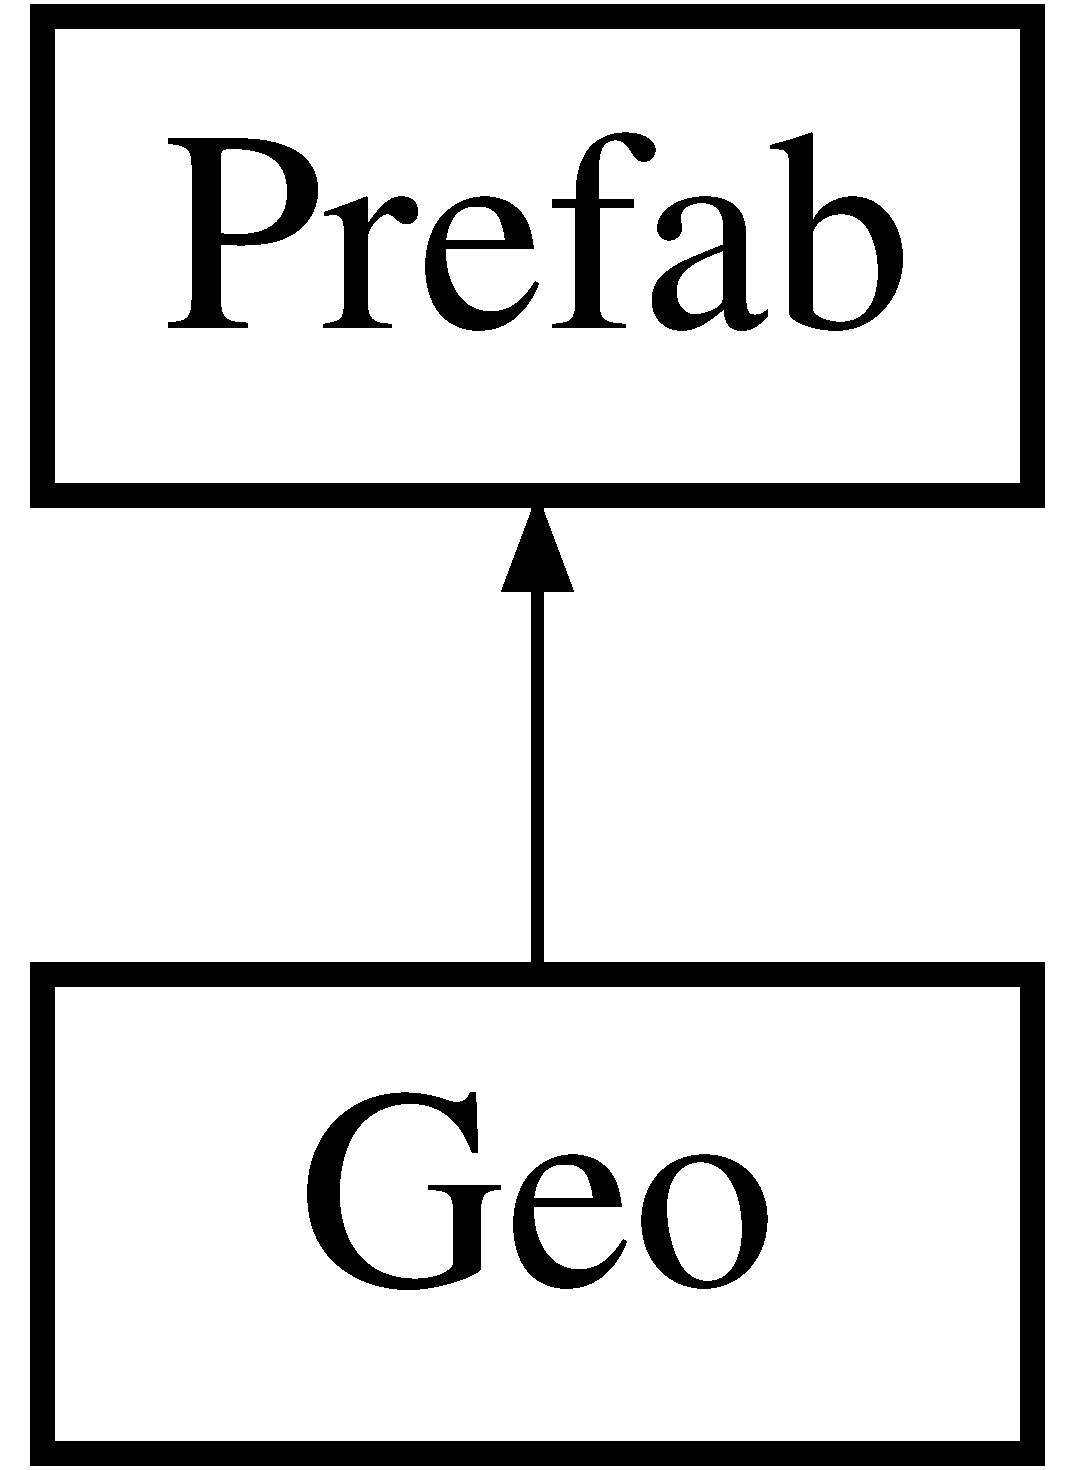
\includegraphics[height=2.000000cm]{class_web_1_1_geo}
\end{center}
\end{figure}
\subsection*{Public Member Functions}
\begin{DoxyCompactItemize}
\item 
\hyperlink{class_web_1_1_geo_a81cf6bb2edc32c23fb528d32adaac50c}{tzinfo} (\$zone)
\item 
\hyperlink{class_web_1_1_geo_ac49b9e92ee8c7a99f780dcf32d50a588}{location} (\$ip=N\+U\+LL)
\item 
\hyperlink{class_web_1_1_geo_a258565515125ab61c663b70102946129}{weather} (\$latitude, \$longitude, \$key)
\end{DoxyCompactItemize}
\subsection*{Additional Inherited Members}


\subsection{Detailed Description}
\hyperlink{class_web_1_1_geo}{Geo} plug-\/in. 

Definition at line 26 of file geo.\+php.



\subsection{Member Function Documentation}
\hypertarget{class_web_1_1_geo_ac49b9e92ee8c7a99f780dcf32d50a588}{}\label{class_web_1_1_geo_ac49b9e92ee8c7a99f780dcf32d50a588} 
\index{Web\+::\+Geo@{Web\+::\+Geo}!location@{location}}
\index{location@{location}!Web\+::\+Geo@{Web\+::\+Geo}}
\subsubsection{\texorpdfstring{location()}{location()}}
{\footnotesize\ttfamily location (\begin{DoxyParamCaption}\item[{}]{\$ip = {\ttfamily NULL} }\end{DoxyParamCaption})}

Return geolocation data based on specified/auto-\/detected IP address \begin{DoxyReturn}{Returns}
array$\vert$\+F\+A\+L\+SE 
\end{DoxyReturn}

\begin{DoxyParams}{Parameters}
{\em \$ip} & string \\
\hline
\end{DoxyParams}


Definition at line 54 of file geo.\+php.

\hypertarget{class_web_1_1_geo_a81cf6bb2edc32c23fb528d32adaac50c}{}\label{class_web_1_1_geo_a81cf6bb2edc32c23fb528d32adaac50c} 
\index{Web\+::\+Geo@{Web\+::\+Geo}!tzinfo@{tzinfo}}
\index{tzinfo@{tzinfo}!Web\+::\+Geo@{Web\+::\+Geo}}
\subsubsection{\texorpdfstring{tzinfo()}{tzinfo()}}
{\footnotesize\ttfamily tzinfo (\begin{DoxyParamCaption}\item[{}]{\$zone }\end{DoxyParamCaption})}

Return information about specified Unix time zone \begin{DoxyReturn}{Returns}
array 
\end{DoxyReturn}

\begin{DoxyParams}{Parameters}
{\em \$zone} & string \\
\hline
\end{DoxyParams}


Definition at line 33 of file geo.\+php.

\hypertarget{class_web_1_1_geo_a258565515125ab61c663b70102946129}{}\label{class_web_1_1_geo_a258565515125ab61c663b70102946129} 
\index{Web\+::\+Geo@{Web\+::\+Geo}!weather@{weather}}
\index{weather@{weather}!Web\+::\+Geo@{Web\+::\+Geo}}
\subsubsection{\texorpdfstring{weather()}{weather()}}
{\footnotesize\ttfamily weather (\begin{DoxyParamCaption}\item[{}]{\$latitude,  }\item[{}]{\$longitude,  }\item[{}]{\$key }\end{DoxyParamCaption})}

Return weather data based on specified latitude/longitude \begin{DoxyReturn}{Returns}
array$\vert$\+F\+A\+L\+SE 
\end{DoxyReturn}

\begin{DoxyParams}{Parameters}
{\em \$latitude} & float \\
\hline
{\em \$longitude} & float \\
\hline
{\em \$key} & string \\
\hline
\end{DoxyParams}


Definition at line 92 of file geo.\+php.



The documentation for this class was generated from the following file\+:\begin{DoxyCompactItemize}
\item 
/\+Users/aplennevaux/\+G\+I\+T\+H\+U\+B/\+Visionary-\/website/src/vendor/bcosca/fatfree/lib/web/geo.\+php\end{DoxyCompactItemize}

\hypertarget{class_image}{}\section{Image Class Reference}
\label{class_image}\index{Image@{Image}}


\hyperlink{class_image}{Image} manipulation tools.  


\subsection*{Public Member Functions}
\begin{DoxyCompactItemize}
\item 
\hyperlink{class_image_ab2758ab5d8c1d2cd3c4e48b72daed2d9}{rgb} (\$color)
\item 
\hyperlink{class_image_a70a743c63f97d5bbfdb2cdab7d186938}{invert} ()
\item 
\hyperlink{class_image_af571c7cddbd8021822dc8a6c36bd4059}{brightness} (\$level)
\item 
\hyperlink{class_image_a7af23605eb273c1084cbbf092bf69c50}{contrast} (\$level)
\item 
\hyperlink{class_image_acc92bb7ca13df725e80732ca8181a0c2}{grayscale} ()
\item 
\hyperlink{class_image_a7ebc6366f3da2bf2af1608663fdb7a09}{smooth} (\$level)
\item 
\hyperlink{class_image_aabc8c1473621bfe3e064dd0a756c935e}{emboss} ()
\item 
\hyperlink{class_image_a4723159606519b101e408854bc65ee35}{sepia} ()
\item 
\hyperlink{class_image_af2baa228f3e2d08bafa8621d4501b113}{pixelate} (\$size)
\item 
\hyperlink{class_image_acdca850837eae7c01092f833157ace57}{blur} (\$selective=F\+A\+L\+SE)
\item 
\hyperlink{class_image_afc92209cb2a19193d46a9338b13a3bb9}{sketch} ()
\item 
\hyperlink{class_image_a24dbd95e2d9306a1bfe43cc344b8af1d}{hflip} ()
\item 
\hyperlink{class_image_ac7bff34c7bb8af86f020474c2f4f2737}{vflip} ()
\item 
\hyperlink{class_image_a4363bcc58d31e100cc126fafad73ef1a}{crop} (\$x1, \$y1, \$x2, \$y2)
\item 
\hyperlink{class_image_a359458680d67cee8333d7af2f078e859}{resize} (\$\hyperlink{class_image_aac6ce1a0981556eb27334db76b666350}{width}=N\+U\+LL, \$\hyperlink{class_image_a40c074d7d21447265a9ce46470c94414}{height}=N\+U\+LL, \$\hyperlink{class_image_a4363bcc58d31e100cc126fafad73ef1a}{crop}=T\+R\+UE, \$enlarge=T\+R\+UE)
\item 
\hyperlink{class_image_a4295061e879c4cc714213bf14116d346}{rotate} (\$angle)
\item 
\hyperlink{class_image_a8a9ac897190d669360d49849f2fedd4b}{overlay} (\hyperlink{class_image}{Image} \$img, \$align=N\+U\+LL, \$alpha=100)
\item 
\hyperlink{class_image_a21a211586a8f97991d047e17b1b886e2}{identicon} (\$str, \$size=64, \$blocks=4)
\item 
\hyperlink{class_image_a4a77a76c9efebb84729d655f56d405d1}{captcha} (\$font, \$size=24, \$len=5, \$key=N\+U\+LL, \$path=\textquotesingle{}\textquotesingle{}, \$fg=0x\+F\+F\+F\+F\+F\+F, \$bg=0x000000)
\item 
\hyperlink{class_image_aac6ce1a0981556eb27334db76b666350}{width} ()
\item 
\hyperlink{class_image_a40c074d7d21447265a9ce46470c94414}{height} ()
\item 
\hyperlink{class_image_afde88292c44dc59faf017738dae6dffb}{render} ()
\item 
\hyperlink{class_image_a5bf63e4ac70cfd9d97e3f2eab936ec8b}{dump} ()
\item 
\hyperlink{class_image_a742e8fae78fd74219638525de1271605}{data} ()
\item 
\hyperlink{class_image_afc8a3c62679cf00ade9f15fb2a6d6132}{save} ()
\item 
\hyperlink{class_image_a6c2fdbe1df4f3168e741037c8be1a7c0}{restore} (\$state=1)
\item 
\hyperlink{class_image_a0347027efc0e46047792065615ac94eb}{undo} ()
\item 
\hyperlink{class_image_afab4d10bf39b2e1c9b00b50833b7442a}{load} (\$str)
\item 
\hyperlink{class_image_a57aaf05740138a0cc4719034d5b066ce}{\+\_\+\+\_\+construct} (\$file=N\+U\+LL, \$flag=F\+A\+L\+SE, \$path=N\+U\+LL)
\item 
\hyperlink{class_image_a421831a265621325e1fdd19aace0c758}{\+\_\+\+\_\+destruct} ()
\end{DoxyCompactItemize}
\subsection*{Data Fields}
\begin{DoxyCompactItemize}
\item 
\hypertarget{class_image_a6efc15b5a2314dd4b5aaa556a375c6d6}{}\label{class_image_a6efc15b5a2314dd4b5aaa556a375c6d6} 
\hyperlink{class_image_a6efc15b5a2314dd4b5aaa556a375c6d6}{\$data}
\begin{DoxyCompactList}\small\item\em \hyperlink{class_image}{Image} resource. \end{DoxyCompactList}\item 
\hypertarget{class_image_acf5d6dd3ee125abb9a2523b30bc47d02}{}\label{class_image_acf5d6dd3ee125abb9a2523b30bc47d02} 
\hyperlink{class_image_acf5d6dd3ee125abb9a2523b30bc47d02}{\$flag} =F\+A\+L\+SE
\begin{DoxyCompactList}\small\item\em Enable/disable history. \end{DoxyCompactList}\item 
\hypertarget{class_image_af789423037bbc89dc7c850e761177570}{}\label{class_image_af789423037bbc89dc7c850e761177570} 
\hyperlink{class_image_af789423037bbc89dc7c850e761177570}{\$count} =0
\begin{DoxyCompactList}\small\item\em Filter count. \end{DoxyCompactList}\end{DoxyCompactItemize}
{\bf }\par
\begin{DoxyCompactItemize}
\item 
\hypertarget{class_image_adfd85288bc26eee86aab0d233a2015e9}{}\label{class_image_adfd85288bc26eee86aab0d233a2015e9} 
const {\bfseries E\+\_\+\+Color} =\textquotesingle{}Invalid color specified\+: \%s\textquotesingle{}
\item 
\hypertarget{class_image_ae0c1bddb66851a1c5d4984cf458a005f}{}\label{class_image_ae0c1bddb66851a1c5d4984cf458a005f} 
const {\bfseries E\+\_\+\+File} =\textquotesingle{}File not found\textquotesingle{}
\item 
\hypertarget{class_image_acd0bd9a1f20fc7514da5cdfac2915be4}{}\label{class_image_acd0bd9a1f20fc7514da5cdfac2915be4} 
const {\bfseries E\+\_\+\+Font} =\textquotesingle{}C\+A\+P\+T\+C\+HA font not found\textquotesingle{}
\item 
\hypertarget{class_image_a44c38043df185dc80b11a79ce277812c}{}\label{class_image_a44c38043df185dc80b11a79ce277812c} 
const {\bfseries E\+\_\+\+T\+TF} =\textquotesingle{}No True\+Type support in GD module\textquotesingle{}
\item 
\hypertarget{class_image_a7b6dc599dc1deedc879b3513186f3ccf}{}\label{class_image_a7b6dc599dc1deedc879b3513186f3ccf} 
const {\bfseries E\+\_\+\+Length} =\textquotesingle{}Invalid C\+A\+P\+T\+C\+HA length\+: \%s\textquotesingle{}
\end{DoxyCompactItemize}

{\bf }\par
\begin{DoxyCompactItemize}
\item 
\hypertarget{class_image_ab225040ebf6e263af6bbcd1499667e24}{}\label{class_image_ab225040ebf6e263af6bbcd1499667e24} 
const {\bfseries P\+O\+S\+\_\+\+Left} =1
\item 
\hypertarget{class_image_ae420359b7aab55c02b2165226f37b596}{}\label{class_image_ae420359b7aab55c02b2165226f37b596} 
const {\bfseries P\+O\+S\+\_\+\+Center} =2
\item 
\hypertarget{class_image_ab54804feab04fe8feb23d94849510922}{}\label{class_image_ab54804feab04fe8feb23d94849510922} 
const {\bfseries P\+O\+S\+\_\+\+Right} =4
\item 
\hypertarget{class_image_a8e891c95deb74e3fcf51bb8ee1827fb9}{}\label{class_image_a8e891c95deb74e3fcf51bb8ee1827fb9} 
const {\bfseries P\+O\+S\+\_\+\+Top} =8
\item 
\hypertarget{class_image_a339da37dd1c147d0db3947297e843d31}{}\label{class_image_a339da37dd1c147d0db3947297e843d31} 
const {\bfseries P\+O\+S\+\_\+\+Middle} =16
\item 
\hypertarget{class_image_a5bbbe1d9932acfbb292e8c76ff17b263}{}\label{class_image_a5bbbe1d9932acfbb292e8c76ff17b263} 
const {\bfseries P\+O\+S\+\_\+\+Bottom} =32
\end{DoxyCompactItemize}

\subsection*{Protected Attributes}
\begin{DoxyCompactItemize}
\item 
\hypertarget{class_image_aa1bfbd27060176201b271918dff57e8f}{}\label{class_image_aa1bfbd27060176201b271918dff57e8f} 
\hyperlink{class_image_aa1bfbd27060176201b271918dff57e8f}{\$file}
\begin{DoxyCompactList}\small\item\em Source filename. \end{DoxyCompactList}\end{DoxyCompactItemize}


\subsection{Detailed Description}
\hyperlink{class_image}{Image} manipulation tools. 

Definition at line 24 of file image.\+php.



\subsection{Constructor \& Destructor Documentation}
\hypertarget{class_image_a57aaf05740138a0cc4719034d5b066ce}{}\label{class_image_a57aaf05740138a0cc4719034d5b066ce} 
\index{Image@{Image}!\+\_\+\+\_\+construct@{\+\_\+\+\_\+construct}}
\index{\+\_\+\+\_\+construct@{\+\_\+\+\_\+construct}!Image@{Image}}
\subsubsection{\texorpdfstring{\+\_\+\+\_\+construct()}{\_\_construct()}}
{\footnotesize\ttfamily \+\_\+\+\_\+construct (\begin{DoxyParamCaption}\item[{}]{\$file = {\ttfamily NULL},  }\item[{}]{\$flag = {\ttfamily FALSE},  }\item[{}]{\$path = {\ttfamily NULL} }\end{DoxyParamCaption})}

Instantiate image 
\begin{DoxyParams}{Parameters}
{\em \$file} & string \\
\hline
{\em \$flag} & bool \\
\hline
{\em \$path} & string \\
\hline
\end{DoxyParams}


Definition at line 585 of file image.\+php.

\hypertarget{class_image_a421831a265621325e1fdd19aace0c758}{}\label{class_image_a421831a265621325e1fdd19aace0c758} 
\index{Image@{Image}!\+\_\+\+\_\+destruct@{\+\_\+\+\_\+destruct}}
\index{\+\_\+\+\_\+destruct@{\+\_\+\+\_\+destruct}!Image@{Image}}
\subsubsection{\texorpdfstring{\+\_\+\+\_\+destruct()}{\_\_destruct()}}
{\footnotesize\ttfamily \+\_\+\+\_\+destruct (\begin{DoxyParamCaption}{ }\end{DoxyParamCaption})}

Wrap-\/up \begin{DoxyReturn}{Returns}
N\+U\+LL 
\end{DoxyReturn}


Definition at line 604 of file image.\+php.



\subsection{Member Function Documentation}
\hypertarget{class_image_acdca850837eae7c01092f833157ace57}{}\label{class_image_acdca850837eae7c01092f833157ace57} 
\index{Image@{Image}!blur@{blur}}
\index{blur@{blur}!Image@{Image}}
\subsubsection{\texorpdfstring{blur()}{blur()}}
{\footnotesize\ttfamily blur (\begin{DoxyParamCaption}\item[{}]{\$selective = {\ttfamily FALSE} }\end{DoxyParamCaption})}

Blur the image using Gaussian filter \begin{DoxyReturn}{Returns}
object 
\end{DoxyReturn}

\begin{DoxyParams}{Parameters}
{\em \$selective} & bool \\
\hline
\end{DoxyParams}


Definition at line 156 of file image.\+php.

\hypertarget{class_image_af571c7cddbd8021822dc8a6c36bd4059}{}\label{class_image_af571c7cddbd8021822dc8a6c36bd4059} 
\index{Image@{Image}!brightness@{brightness}}
\index{brightness@{brightness}!Image@{Image}}
\subsubsection{\texorpdfstring{brightness()}{brightness()}}
{\footnotesize\ttfamily brightness (\begin{DoxyParamCaption}\item[{}]{\$level }\end{DoxyParamCaption})}

Adjust brightness (range\+:-\/255 to 255) \begin{DoxyReturn}{Returns}
object 
\end{DoxyReturn}

\begin{DoxyParams}{Parameters}
{\em \$level} & int \\
\hline
\end{DoxyParams}


Definition at line 88 of file image.\+php.

\hypertarget{class_image_a4a77a76c9efebb84729d655f56d405d1}{}\label{class_image_a4a77a76c9efebb84729d655f56d405d1} 
\index{Image@{Image}!captcha@{captcha}}
\index{captcha@{captcha}!Image@{Image}}
\subsubsection{\texorpdfstring{captcha()}{captcha()}}
{\footnotesize\ttfamily captcha (\begin{DoxyParamCaption}\item[{}]{\$font,  }\item[{}]{\$size = {\ttfamily 24},  }\item[{}]{\$len = {\ttfamily 5},  }\item[{}]{\$key = {\ttfamily NULL},  }\item[{}]{\$path = {\ttfamily \textquotesingle{}\textquotesingle{}},  }\item[{}]{\$fg = {\ttfamily 0xFFFFFF},  }\item[{}]{\$bg = {\ttfamily 0x000000} }\end{DoxyParamCaption})}

Generate C\+A\+P\+T\+C\+HA image \begin{DoxyReturn}{Returns}
object$\vert$\+F\+A\+L\+SE 
\end{DoxyReturn}

\begin{DoxyParams}{Parameters}
{\em \$font} & string \\
\hline
{\em \$size} & int \\
\hline
{\em \$len} & int \\
\hline
{\em \$key} & string \\
\hline
{\em \$path} & string \\
\hline
{\em \$fg} & int \\
\hline
{\em \$bg} & int \\
\hline
\end{DoxyParams}


Definition at line 401 of file image.\+php.

\hypertarget{class_image_a7af23605eb273c1084cbbf092bf69c50}{}\label{class_image_a7af23605eb273c1084cbbf092bf69c50} 
\index{Image@{Image}!contrast@{contrast}}
\index{contrast@{contrast}!Image@{Image}}
\subsubsection{\texorpdfstring{contrast()}{contrast()}}
{\footnotesize\ttfamily contrast (\begin{DoxyParamCaption}\item[{}]{\$level }\end{DoxyParamCaption})}

Adjust contrast (range\+:-\/100 to 100) \begin{DoxyReturn}{Returns}
object 
\end{DoxyReturn}

\begin{DoxyParams}{Parameters}
{\em \$level} & int \\
\hline
\end{DoxyParams}


Definition at line 98 of file image.\+php.

\hypertarget{class_image_a4363bcc58d31e100cc126fafad73ef1a}{}\label{class_image_a4363bcc58d31e100cc126fafad73ef1a} 
\index{Image@{Image}!crop@{crop}}
\index{crop@{crop}!Image@{Image}}
\subsubsection{\texorpdfstring{crop()}{crop()}}
{\footnotesize\ttfamily crop (\begin{DoxyParamCaption}\item[{}]{\$x1,  }\item[{}]{\$y1,  }\item[{}]{\$x2,  }\item[{}]{\$y2 }\end{DoxyParamCaption})}

Crop the image \begin{DoxyReturn}{Returns}
object 
\end{DoxyReturn}

\begin{DoxyParams}{Parameters}
{\em \$x1} & int \\
\hline
{\em \$y1} & int \\
\hline
{\em \$x2} & int \\
\hline
{\em \$y2} & int \\
\hline
\end{DoxyParams}


Definition at line 211 of file image.\+php.

\hypertarget{class_image_a742e8fae78fd74219638525de1271605}{}\label{class_image_a742e8fae78fd74219638525de1271605} 
\index{Image@{Image}!data@{data}}
\index{data@{data}!Image@{Image}}
\subsubsection{\texorpdfstring{data()}{data()}}
{\footnotesize\ttfamily data (\begin{DoxyParamCaption}{ }\end{DoxyParamCaption})}

Return image resource \begin{DoxyReturn}{Returns}
resource 
\end{DoxyReturn}


Definition at line 510 of file image.\+php.

\hypertarget{class_image_a5bf63e4ac70cfd9d97e3f2eab936ec8b}{}\label{class_image_a5bf63e4ac70cfd9d97e3f2eab936ec8b} 
\index{Image@{Image}!dump@{dump}}
\index{dump@{dump}!Image@{Image}}
\subsubsection{\texorpdfstring{dump()}{dump()}}
{\footnotesize\ttfamily dump (\begin{DoxyParamCaption}{ }\end{DoxyParamCaption})}

Return image as a string \begin{DoxyReturn}{Returns}
string 
\end{DoxyReturn}


Definition at line 495 of file image.\+php.

\hypertarget{class_image_aabc8c1473621bfe3e064dd0a756c935e}{}\label{class_image_aabc8c1473621bfe3e064dd0a756c935e} 
\index{Image@{Image}!emboss@{emboss}}
\index{emboss@{emboss}!Image@{Image}}
\subsubsection{\texorpdfstring{emboss()}{emboss()}}
{\footnotesize\ttfamily emboss (\begin{DoxyParamCaption}{ }\end{DoxyParamCaption})}

Emboss the image \begin{DoxyReturn}{Returns}
object 
\end{DoxyReturn}


Definition at line 126 of file image.\+php.

\hypertarget{class_image_acc92bb7ca13df725e80732ca8181a0c2}{}\label{class_image_acc92bb7ca13df725e80732ca8181a0c2} 
\index{Image@{Image}!grayscale@{grayscale}}
\index{grayscale@{grayscale}!Image@{Image}}
\subsubsection{\texorpdfstring{grayscale()}{grayscale()}}
{\footnotesize\ttfamily grayscale (\begin{DoxyParamCaption}{ }\end{DoxyParamCaption})}

Convert to grayscale \begin{DoxyReturn}{Returns}
object 
\end{DoxyReturn}


Definition at line 107 of file image.\+php.

\hypertarget{class_image_a40c074d7d21447265a9ce46470c94414}{}\label{class_image_a40c074d7d21447265a9ce46470c94414} 
\index{Image@{Image}!height@{height}}
\index{height@{height}!Image@{Image}}
\subsubsection{\texorpdfstring{height()}{height()}}
{\footnotesize\ttfamily height (\begin{DoxyParamCaption}{ }\end{DoxyParamCaption})}

Return image height \begin{DoxyReturn}{Returns}
int 
\end{DoxyReturn}


Definition at line 470 of file image.\+php.

\hypertarget{class_image_a24dbd95e2d9306a1bfe43cc344b8af1d}{}\label{class_image_a24dbd95e2d9306a1bfe43cc344b8af1d} 
\index{Image@{Image}!hflip@{hflip}}
\index{hflip@{hflip}!Image@{Image}}
\subsubsection{\texorpdfstring{hflip()}{hflip()}}
{\footnotesize\ttfamily hflip (\begin{DoxyParamCaption}{ }\end{DoxyParamCaption})}

Flip on horizontal axis \begin{DoxyReturn}{Returns}
object 
\end{DoxyReturn}


Definition at line 175 of file image.\+php.

\hypertarget{class_image_a21a211586a8f97991d047e17b1b886e2}{}\label{class_image_a21a211586a8f97991d047e17b1b886e2} 
\index{Image@{Image}!identicon@{identicon}}
\index{identicon@{identicon}!Image@{Image}}
\subsubsection{\texorpdfstring{identicon()}{identicon()}}
{\footnotesize\ttfamily identicon (\begin{DoxyParamCaption}\item[{}]{\$str,  }\item[{}]{\$size = {\ttfamily 64},  }\item[{}]{\$blocks = {\ttfamily 4} }\end{DoxyParamCaption})}

Generate identicon \begin{DoxyReturn}{Returns}
object 
\end{DoxyReturn}

\begin{DoxyParams}{Parameters}
{\em \$str} & string \\
\hline
{\em \$size} & int \\
\hline
{\em \$blocks} & int \\
\hline
\end{DoxyParams}


Definition at line 344 of file image.\+php.

\hypertarget{class_image_a70a743c63f97d5bbfdb2cdab7d186938}{}\label{class_image_a70a743c63f97d5bbfdb2cdab7d186938} 
\index{Image@{Image}!invert@{invert}}
\index{invert@{invert}!Image@{Image}}
\subsubsection{\texorpdfstring{invert()}{invert()}}
{\footnotesize\ttfamily invert (\begin{DoxyParamCaption}{ }\end{DoxyParamCaption})}

Invert image \begin{DoxyReturn}{Returns}
object 
\end{DoxyReturn}


Definition at line 78 of file image.\+php.

\hypertarget{class_image_afab4d10bf39b2e1c9b00b50833b7442a}{}\label{class_image_afab4d10bf39b2e1c9b00b50833b7442a} 
\index{Image@{Image}!load@{load}}
\index{load@{load}!Image@{Image}}
\subsubsection{\texorpdfstring{load()}{load()}}
{\footnotesize\ttfamily load (\begin{DoxyParamCaption}\item[{}]{\$str }\end{DoxyParamCaption})}

Load string \begin{DoxyReturn}{Returns}
object$\vert$\+F\+A\+L\+SE 
\end{DoxyReturn}

\begin{DoxyParams}{Parameters}
{\em \$str} & string \\
\hline
\end{DoxyParams}


Definition at line 571 of file image.\+php.

\hypertarget{class_image_a8a9ac897190d669360d49849f2fedd4b}{}\label{class_image_a8a9ac897190d669360d49849f2fedd4b} 
\index{Image@{Image}!overlay@{overlay}}
\index{overlay@{overlay}!Image@{Image}}
\subsubsection{\texorpdfstring{overlay()}{overlay()}}
{\footnotesize\ttfamily overlay (\begin{DoxyParamCaption}\item[{\hyperlink{class_image}{Image}}]{\$img,  }\item[{}]{\$align = {\ttfamily NULL},  }\item[{}]{\$alpha = {\ttfamily 100} }\end{DoxyParamCaption})}

Apply an image overlay \begin{DoxyReturn}{Returns}
object 
\end{DoxyReturn}

\begin{DoxyParams}{Parameters}
{\em \$img} & object \\
\hline
{\em \$align} & int$\vert$array \\
\hline
{\em \$alpha} & int \\
\hline
\end{DoxyParams}


Definition at line 296 of file image.\+php.

\hypertarget{class_image_af2baa228f3e2d08bafa8621d4501b113}{}\label{class_image_af2baa228f3e2d08bafa8621d4501b113} 
\index{Image@{Image}!pixelate@{pixelate}}
\index{pixelate@{pixelate}!Image@{Image}}
\subsubsection{\texorpdfstring{pixelate()}{pixelate()}}
{\footnotesize\ttfamily pixelate (\begin{DoxyParamCaption}\item[{}]{\$size }\end{DoxyParamCaption})}

Pixelate the image \begin{DoxyReturn}{Returns}
object 
\end{DoxyReturn}

\begin{DoxyParams}{Parameters}
{\em \$size} & int \\
\hline
\end{DoxyParams}


Definition at line 146 of file image.\+php.

\hypertarget{class_image_afde88292c44dc59faf017738dae6dffb}{}\label{class_image_afde88292c44dc59faf017738dae6dffb} 
\index{Image@{Image}!render@{render}}
\index{render@{render}!Image@{Image}}
\subsubsection{\texorpdfstring{render()}{render()}}
{\footnotesize\ttfamily render (\begin{DoxyParamCaption}{ }\end{DoxyParamCaption})}

Send image to H\+T\+TP client \begin{DoxyReturn}{Returns}
N\+U\+LL 
\end{DoxyReturn}


Definition at line 478 of file image.\+php.

\hypertarget{class_image_a359458680d67cee8333d7af2f078e859}{}\label{class_image_a359458680d67cee8333d7af2f078e859} 
\index{Image@{Image}!resize@{resize}}
\index{resize@{resize}!Image@{Image}}
\subsubsection{\texorpdfstring{resize()}{resize()}}
{\footnotesize\ttfamily resize (\begin{DoxyParamCaption}\item[{}]{\$width = {\ttfamily NULL},  }\item[{}]{\$height = {\ttfamily NULL},  }\item[{}]{\$crop = {\ttfamily TRUE},  }\item[{}]{\$enlarge = {\ttfamily TRUE} }\end{DoxyParamCaption})}

Resize image (Maintain aspect ratio); Crop relative to center if flag is enabled; Enlargement allowed if flag is enabled \begin{DoxyReturn}{Returns}
object 
\end{DoxyReturn}

\begin{DoxyParams}{Parameters}
{\em \$width} & int \\
\hline
{\em \$height} & int \\
\hline
{\em \$crop} & bool \\
\hline
{\em \$enlarge} & bool \\
\hline
\end{DoxyParams}


Definition at line 231 of file image.\+php.

\hypertarget{class_image_a6c2fdbe1df4f3168e741037c8be1a7c0}{}\label{class_image_a6c2fdbe1df4f3168e741037c8be1a7c0} 
\index{Image@{Image}!restore@{restore}}
\index{restore@{restore}!Image@{Image}}
\subsubsection{\texorpdfstring{restore()}{restore()}}
{\footnotesize\ttfamily restore (\begin{DoxyParamCaption}\item[{}]{\$state = {\ttfamily 1} }\end{DoxyParamCaption})}

Revert to specified state \begin{DoxyReturn}{Returns}
object 
\end{DoxyReturn}

\begin{DoxyParams}{Parameters}
{\em \$state} & int \\
\hline
\end{DoxyParams}


Definition at line 536 of file image.\+php.

\hypertarget{class_image_ab2758ab5d8c1d2cd3c4e48b72daed2d9}{}\label{class_image_ab2758ab5d8c1d2cd3c4e48b72daed2d9} 
\index{Image@{Image}!rgb@{rgb}}
\index{rgb@{rgb}!Image@{Image}}
\subsubsection{\texorpdfstring{rgb()}{rgb()}}
{\footnotesize\ttfamily rgb (\begin{DoxyParamCaption}\item[{}]{\$color }\end{DoxyParamCaption})}

Convert R\+GB hex triad to array \begin{DoxyReturn}{Returns}
array$\vert$\+F\+A\+L\+SE 
\end{DoxyReturn}

\begin{DoxyParams}{Parameters}
{\em \$color} & int$\vert$string \\
\hline
\end{DoxyParams}


Definition at line 60 of file image.\+php.

\hypertarget{class_image_a4295061e879c4cc714213bf14116d346}{}\label{class_image_a4295061e879c4cc714213bf14116d346} 
\index{Image@{Image}!rotate@{rotate}}
\index{rotate@{rotate}!Image@{Image}}
\subsubsection{\texorpdfstring{rotate()}{rotate()}}
{\footnotesize\ttfamily rotate (\begin{DoxyParamCaption}\item[{}]{\$angle }\end{DoxyParamCaption})}

Rotate image \begin{DoxyReturn}{Returns}
object 
\end{DoxyReturn}

\begin{DoxyParams}{Parameters}
{\em \$angle} & int \\
\hline
\end{DoxyParams}


Definition at line 282 of file image.\+php.

\hypertarget{class_image_afc8a3c62679cf00ade9f15fb2a6d6132}{}\label{class_image_afc8a3c62679cf00ade9f15fb2a6d6132} 
\index{Image@{Image}!save@{save}}
\index{save@{save}!Image@{Image}}
\subsubsection{\texorpdfstring{save()}{save()}}
{\footnotesize\ttfamily save (\begin{DoxyParamCaption}{ }\end{DoxyParamCaption})}

Save current state \begin{DoxyReturn}{Returns}
object 
\end{DoxyReturn}


Definition at line 518 of file image.\+php.

\hypertarget{class_image_a4723159606519b101e408854bc65ee35}{}\label{class_image_a4723159606519b101e408854bc65ee35} 
\index{Image@{Image}!sepia@{sepia}}
\index{sepia@{sepia}!Image@{Image}}
\subsubsection{\texorpdfstring{sepia()}{sepia()}}
{\footnotesize\ttfamily sepia (\begin{DoxyParamCaption}{ }\end{DoxyParamCaption})}

Apply sepia effect \begin{DoxyReturn}{Returns}
object 
\end{DoxyReturn}


Definition at line 135 of file image.\+php.

\hypertarget{class_image_afc92209cb2a19193d46a9338b13a3bb9}{}\label{class_image_afc92209cb2a19193d46a9338b13a3bb9} 
\index{Image@{Image}!sketch@{sketch}}
\index{sketch@{sketch}!Image@{Image}}
\subsubsection{\texorpdfstring{sketch()}{sketch()}}
{\footnotesize\ttfamily sketch (\begin{DoxyParamCaption}{ }\end{DoxyParamCaption})}

Apply sketch effect \begin{DoxyReturn}{Returns}
object 
\end{DoxyReturn}


Definition at line 166 of file image.\+php.

\hypertarget{class_image_a7ebc6366f3da2bf2af1608663fdb7a09}{}\label{class_image_a7ebc6366f3da2bf2af1608663fdb7a09} 
\index{Image@{Image}!smooth@{smooth}}
\index{smooth@{smooth}!Image@{Image}}
\subsubsection{\texorpdfstring{smooth()}{smooth()}}
{\footnotesize\ttfamily smooth (\begin{DoxyParamCaption}\item[{}]{\$level }\end{DoxyParamCaption})}

Adjust smoothness \begin{DoxyReturn}{Returns}
object 
\end{DoxyReturn}

\begin{DoxyParams}{Parameters}
{\em \$level} & int \\
\hline
\end{DoxyParams}


Definition at line 117 of file image.\+php.

\hypertarget{class_image_a0347027efc0e46047792065615ac94eb}{}\label{class_image_a0347027efc0e46047792065615ac94eb} 
\index{Image@{Image}!undo@{undo}}
\index{undo@{undo}!Image@{Image}}
\subsubsection{\texorpdfstring{undo()}{undo()}}
{\footnotesize\ttfamily undo (\begin{DoxyParamCaption}{ }\end{DoxyParamCaption})}

Undo most recently applied filter \begin{DoxyReturn}{Returns}
object 
\end{DoxyReturn}


Definition at line 557 of file image.\+php.

\hypertarget{class_image_ac7bff34c7bb8af86f020474c2f4f2737}{}\label{class_image_ac7bff34c7bb8af86f020474c2f4f2737} 
\index{Image@{Image}!vflip@{vflip}}
\index{vflip@{vflip}!Image@{Image}}
\subsubsection{\texorpdfstring{vflip()}{vflip()}}
{\footnotesize\ttfamily vflip (\begin{DoxyParamCaption}{ }\end{DoxyParamCaption})}

Flip on vertical axis \begin{DoxyReturn}{Returns}
object 
\end{DoxyReturn}


Definition at line 191 of file image.\+php.

\hypertarget{class_image_aac6ce1a0981556eb27334db76b666350}{}\label{class_image_aac6ce1a0981556eb27334db76b666350} 
\index{Image@{Image}!width@{width}}
\index{width@{width}!Image@{Image}}
\subsubsection{\texorpdfstring{width()}{width()}}
{\footnotesize\ttfamily width (\begin{DoxyParamCaption}{ }\end{DoxyParamCaption})}

Return image width \begin{DoxyReturn}{Returns}
int 
\end{DoxyReturn}


Definition at line 462 of file image.\+php.



The documentation for this class was generated from the following file\+:\begin{DoxyCompactItemize}
\item 
/\+Users/aplennevaux/\+G\+I\+T\+H\+U\+B/\+Visionary-\/website/src/vendor/bcosca/fatfree/lib/image.\+php\end{DoxyCompactItemize}

\hypertarget{class_i_s_o}{}\section{I\+SO Class Reference}
\label{class_i_s_o}\index{I\+SO@{I\+SO}}


\hyperlink{class_i_s_o}{I\+SO} language/country codes.  


Inheritance diagram for I\+SO\+:\begin{figure}[H]
\begin{center}
\leavevmode
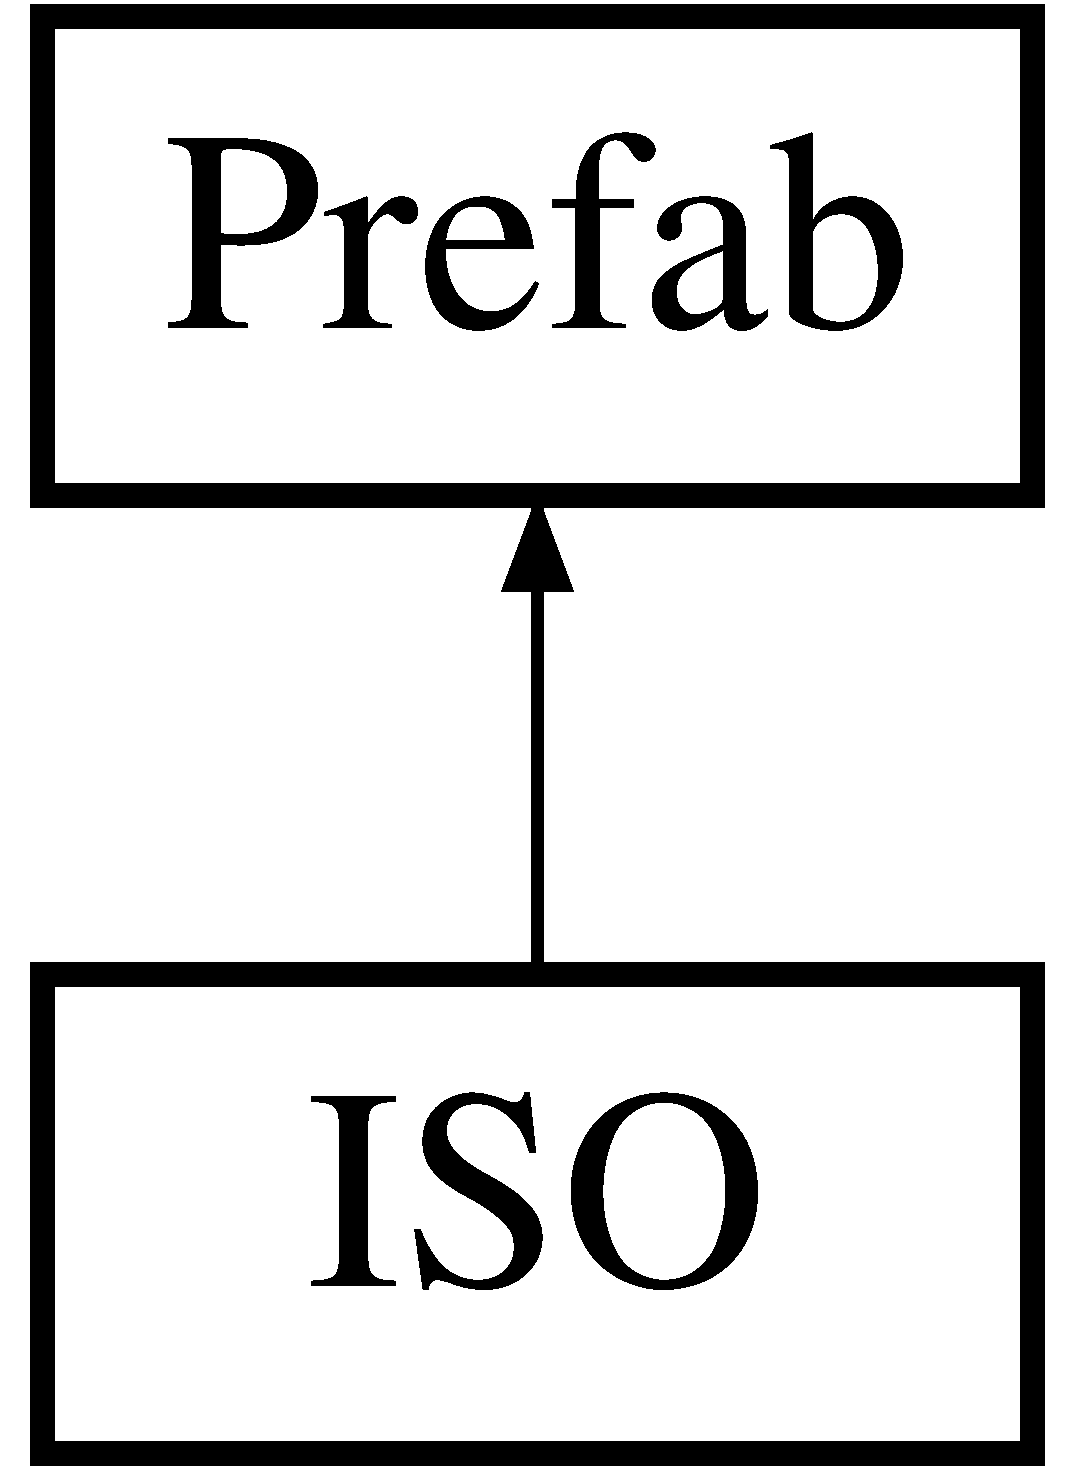
\includegraphics[height=2.000000cm]{class_i_s_o}
\end{center}
\end{figure}
\subsection*{Public Member Functions}
\begin{DoxyCompactItemize}
\item 
\hyperlink{class_i_s_o_adda8fc15b6fe0efc05a50d2645189c77}{languages} ()
\item 
\hyperlink{class_i_s_o_a662d2f9a4067a75b295cff7ff65d658f}{countries} ()
\end{DoxyCompactItemize}
\subsection*{Data Fields}
{\bf }\par
\begin{DoxyCompactItemize}
\item 
\hypertarget{class_i_s_o_aba79ec023836cd11ff49dda6cddd675b}{}\label{class_i_s_o_aba79ec023836cd11ff49dda6cddd675b} 
const {\bfseries C\+C\+\_\+af} =\textquotesingle{}Afghanistan\textquotesingle{}
\item 
\hypertarget{class_i_s_o_acfff7c05938b3bbfe387d090ad4c03e9}{}\label{class_i_s_o_acfff7c05938b3bbfe387d090ad4c03e9} 
const {\bfseries C\+C\+\_\+ax} =\textquotesingle{}Åland Islands\textquotesingle{}
\item 
\hypertarget{class_i_s_o_a92df0696009b43de051daab0bfef9a63}{}\label{class_i_s_o_a92df0696009b43de051daab0bfef9a63} 
const {\bfseries C\+C\+\_\+al} =\textquotesingle{}Albania\textquotesingle{}
\item 
\hypertarget{class_i_s_o_aa5f7590dcf123a99b4a6c9c183374441}{}\label{class_i_s_o_aa5f7590dcf123a99b4a6c9c183374441} 
const {\bfseries C\+C\+\_\+dz} =\textquotesingle{}Algeria\textquotesingle{}
\item 
\hypertarget{class_i_s_o_a3c7cdf2bdd1fef75cc5066dfa6ae8af7}{}\label{class_i_s_o_a3c7cdf2bdd1fef75cc5066dfa6ae8af7} 
const {\bfseries C\+C\+\_\+as} =\textquotesingle{}American Samoa\textquotesingle{}
\item 
\hypertarget{class_i_s_o_ade941d67f08b82af4c77284d8151c0bb}{}\label{class_i_s_o_ade941d67f08b82af4c77284d8151c0bb} 
const {\bfseries C\+C\+\_\+ad} =\textquotesingle{}Andorra\textquotesingle{}
\item 
\hypertarget{class_i_s_o_a8c4d71031d389c152f729474cc723faa}{}\label{class_i_s_o_a8c4d71031d389c152f729474cc723faa} 
const {\bfseries C\+C\+\_\+ao} =\textquotesingle{}Angola\textquotesingle{}
\item 
\hypertarget{class_i_s_o_a45e9d4e3f3135e4c5b539b210de3a9d3}{}\label{class_i_s_o_a45e9d4e3f3135e4c5b539b210de3a9d3} 
const {\bfseries C\+C\+\_\+ai} =\textquotesingle{}Anguilla\textquotesingle{}
\item 
\hypertarget{class_i_s_o_a51124935ab9cead4875ee036e14e402a}{}\label{class_i_s_o_a51124935ab9cead4875ee036e14e402a} 
const {\bfseries C\+C\+\_\+aq} =\textquotesingle{}Antarctica\textquotesingle{}
\item 
\hypertarget{class_i_s_o_a180a206b0f6d62304d50e7c05be23c11}{}\label{class_i_s_o_a180a206b0f6d62304d50e7c05be23c11} 
const {\bfseries C\+C\+\_\+ag} =\textquotesingle{}Antigua and Barbuda\textquotesingle{}
\item 
\hypertarget{class_i_s_o_abb102cc6e2b6471d3b0dff1700798a73}{}\label{class_i_s_o_abb102cc6e2b6471d3b0dff1700798a73} 
const {\bfseries C\+C\+\_\+ar} =\textquotesingle{}Argentina\textquotesingle{}
\item 
\hypertarget{class_i_s_o_a3d334d544ffb9fad3b09fc2ee8c4643a}{}\label{class_i_s_o_a3d334d544ffb9fad3b09fc2ee8c4643a} 
const {\bfseries C\+C\+\_\+am} =\textquotesingle{}Armenia\textquotesingle{}
\item 
\hypertarget{class_i_s_o_afd4252c9381c37e569417b764021fcae}{}\label{class_i_s_o_afd4252c9381c37e569417b764021fcae} 
const {\bfseries C\+C\+\_\+aw} =\textquotesingle{}Aruba\textquotesingle{}
\item 
\hypertarget{class_i_s_o_a68e88bbdbd60df04ed5d61b21fc914e0}{}\label{class_i_s_o_a68e88bbdbd60df04ed5d61b21fc914e0} 
const {\bfseries C\+C\+\_\+au} =\textquotesingle{}Australia\textquotesingle{}
\item 
\hypertarget{class_i_s_o_a55a9f9dd8c9db9f627b44ae2b51d4bbe}{}\label{class_i_s_o_a55a9f9dd8c9db9f627b44ae2b51d4bbe} 
const {\bfseries C\+C\+\_\+at} =\textquotesingle{}Austria\textquotesingle{}
\item 
\hypertarget{class_i_s_o_a0d74302b6664d7eef3063f135416e761}{}\label{class_i_s_o_a0d74302b6664d7eef3063f135416e761} 
const {\bfseries C\+C\+\_\+az} =\textquotesingle{}Azerbaijan\textquotesingle{}
\item 
\hypertarget{class_i_s_o_a14dd595f01bad4847a22d20daf7d0b59}{}\label{class_i_s_o_a14dd595f01bad4847a22d20daf7d0b59} 
const {\bfseries C\+C\+\_\+bs} =\textquotesingle{}Bahamas\textquotesingle{}
\item 
\hypertarget{class_i_s_o_a7b66f05bf64ff30e8df55f25770c070f}{}\label{class_i_s_o_a7b66f05bf64ff30e8df55f25770c070f} 
const {\bfseries C\+C\+\_\+bh} =\textquotesingle{}Bahrain\textquotesingle{}
\item 
\hypertarget{class_i_s_o_a7a161434d5d6b9f160f1229024a2a0ec}{}\label{class_i_s_o_a7a161434d5d6b9f160f1229024a2a0ec} 
const {\bfseries C\+C\+\_\+bd} =\textquotesingle{}Bangladesh\textquotesingle{}
\item 
\hypertarget{class_i_s_o_a309019f8c2b554d310a839cf28f8463d}{}\label{class_i_s_o_a309019f8c2b554d310a839cf28f8463d} 
const {\bfseries C\+C\+\_\+bb} =\textquotesingle{}Barbados\textquotesingle{}
\item 
\hypertarget{class_i_s_o_a2277e57130c66d4ccc0bcf0c3ca830a2}{}\label{class_i_s_o_a2277e57130c66d4ccc0bcf0c3ca830a2} 
const {\bfseries C\+C\+\_\+by} =\textquotesingle{}Belarus\textquotesingle{}
\item 
\hypertarget{class_i_s_o_a37e3e4c86d8a48574833899497b14cec}{}\label{class_i_s_o_a37e3e4c86d8a48574833899497b14cec} 
const {\bfseries C\+C\+\_\+be} =\textquotesingle{}Belgium\textquotesingle{}
\item 
\hypertarget{class_i_s_o_acffaaa157ec8a86e9ac82ad657552a5f}{}\label{class_i_s_o_acffaaa157ec8a86e9ac82ad657552a5f} 
const {\bfseries C\+C\+\_\+bz} =\textquotesingle{}Belize\textquotesingle{}
\item 
\hypertarget{class_i_s_o_aa577cece1733a86a1e013095b94c7e96}{}\label{class_i_s_o_aa577cece1733a86a1e013095b94c7e96} 
const {\bfseries C\+C\+\_\+bj} =\textquotesingle{}Benin\textquotesingle{}
\item 
\hypertarget{class_i_s_o_a4dc1d37b66e0ff75d1a1d0995ffadb3b}{}\label{class_i_s_o_a4dc1d37b66e0ff75d1a1d0995ffadb3b} 
const {\bfseries C\+C\+\_\+bm} =\textquotesingle{}Bermuda\textquotesingle{}
\item 
\hypertarget{class_i_s_o_a5daf301b5d449cbc01c064873382e600}{}\label{class_i_s_o_a5daf301b5d449cbc01c064873382e600} 
const {\bfseries C\+C\+\_\+bt} =\textquotesingle{}Bhutan\textquotesingle{}
\item 
\hypertarget{class_i_s_o_a92393ac5e7aac27c1fd4158d5d0d1832}{}\label{class_i_s_o_a92393ac5e7aac27c1fd4158d5d0d1832} 
const {\bfseries C\+C\+\_\+bo} =\textquotesingle{}Bolivia\textquotesingle{}
\item 
\hypertarget{class_i_s_o_ae092ddfc96ee8c9b41247a7b2e023597}{}\label{class_i_s_o_ae092ddfc96ee8c9b41247a7b2e023597} 
const {\bfseries C\+C\+\_\+bq} =\textquotesingle{}Bonaire, Sint Eustatius and Saba\textquotesingle{}
\item 
\hypertarget{class_i_s_o_a20aa41a46ef319522bad220e6e998db5}{}\label{class_i_s_o_a20aa41a46ef319522bad220e6e998db5} 
const {\bfseries C\+C\+\_\+ba} =\textquotesingle{}Bosnia and Herzegovina\textquotesingle{}
\item 
\hypertarget{class_i_s_o_a75d004663f195bfb2623e58f0e20a083}{}\label{class_i_s_o_a75d004663f195bfb2623e58f0e20a083} 
const {\bfseries C\+C\+\_\+bw} =\textquotesingle{}Botswana\textquotesingle{}
\item 
\hypertarget{class_i_s_o_aea5bf115700b4c0beeccd6eaf441cc4e}{}\label{class_i_s_o_aea5bf115700b4c0beeccd6eaf441cc4e} 
const {\bfseries C\+C\+\_\+bv} =\textquotesingle{}Bouvet Island\textquotesingle{}
\item 
\hypertarget{class_i_s_o_af1b80f3c67c38253181c33648f8f2fd9}{}\label{class_i_s_o_af1b80f3c67c38253181c33648f8f2fd9} 
const {\bfseries C\+C\+\_\+br} =\textquotesingle{}Brazil\textquotesingle{}
\item 
\hypertarget{class_i_s_o_a9612992591fc481d71d164a891d20ffd}{}\label{class_i_s_o_a9612992591fc481d71d164a891d20ffd} 
const {\bfseries C\+C\+\_\+io} =\textquotesingle{}British Indian Ocean Territory\textquotesingle{}
\item 
\hypertarget{class_i_s_o_a8d3537901fd9f7a04b0b00d03d51e392}{}\label{class_i_s_o_a8d3537901fd9f7a04b0b00d03d51e392} 
const {\bfseries C\+C\+\_\+bn} =\textquotesingle{}Brunei Darussalam\textquotesingle{}
\item 
\hypertarget{class_i_s_o_aa82437be22f8b7f72af24c314655e747}{}\label{class_i_s_o_aa82437be22f8b7f72af24c314655e747} 
const {\bfseries C\+C\+\_\+bg} =\textquotesingle{}Bulgaria\textquotesingle{}
\item 
\hypertarget{class_i_s_o_a33fe546ce28384f1b11d91845b912a95}{}\label{class_i_s_o_a33fe546ce28384f1b11d91845b912a95} 
const {\bfseries C\+C\+\_\+bf} =\textquotesingle{}Burkina Faso\textquotesingle{}
\item 
\hypertarget{class_i_s_o_a551c26da8d3bfdb5269032ccecf630a8}{}\label{class_i_s_o_a551c26da8d3bfdb5269032ccecf630a8} 
const {\bfseries C\+C\+\_\+bi} =\textquotesingle{}Burundi\textquotesingle{}
\item 
\hypertarget{class_i_s_o_af39501ec83776d07cde2b689ae7b50f3}{}\label{class_i_s_o_af39501ec83776d07cde2b689ae7b50f3} 
const {\bfseries C\+C\+\_\+kh} =\textquotesingle{}Cambodia\textquotesingle{}
\item 
\hypertarget{class_i_s_o_aff13938190d5a2453f62d7b40853c610}{}\label{class_i_s_o_aff13938190d5a2453f62d7b40853c610} 
const {\bfseries C\+C\+\_\+cm} =\textquotesingle{}Cameroon\textquotesingle{}
\item 
\hypertarget{class_i_s_o_a9b62191df86333ff4b6deb9dc7566764}{}\label{class_i_s_o_a9b62191df86333ff4b6deb9dc7566764} 
const {\bfseries C\+C\+\_\+ca} =\textquotesingle{}Canada\textquotesingle{}
\item 
\hypertarget{class_i_s_o_a2457c77da85be8baae655bae00f514e7}{}\label{class_i_s_o_a2457c77da85be8baae655bae00f514e7} 
const {\bfseries C\+C\+\_\+cv} =\textquotesingle{}Cape Verde\textquotesingle{}
\item 
\hypertarget{class_i_s_o_ac67fc7612cc1b0e4b3cd6a6c7525b47d}{}\label{class_i_s_o_ac67fc7612cc1b0e4b3cd6a6c7525b47d} 
const {\bfseries C\+C\+\_\+ky} =\textquotesingle{}Cayman Islands\textquotesingle{}
\item 
\hypertarget{class_i_s_o_a3d25c268d084fd4a06f322e80d001adc}{}\label{class_i_s_o_a3d25c268d084fd4a06f322e80d001adc} 
const {\bfseries C\+C\+\_\+cf} =\textquotesingle{}Central African Republic\textquotesingle{}
\item 
\hypertarget{class_i_s_o_a43c439529ab1774b2e5764b1bd8d66c7}{}\label{class_i_s_o_a43c439529ab1774b2e5764b1bd8d66c7} 
const {\bfseries C\+C\+\_\+td} =\textquotesingle{}Chad\textquotesingle{}
\item 
\hypertarget{class_i_s_o_aec418875b0793a704961b274af7c9302}{}\label{class_i_s_o_aec418875b0793a704961b274af7c9302} 
const {\bfseries C\+C\+\_\+cl} =\textquotesingle{}Chile\textquotesingle{}
\item 
\hypertarget{class_i_s_o_af965d0ee53530325499aa679a79cef34}{}\label{class_i_s_o_af965d0ee53530325499aa679a79cef34} 
const {\bfseries C\+C\+\_\+cn} =\textquotesingle{}China\textquotesingle{}
\item 
\hypertarget{class_i_s_o_ac359ab46aff9f8673fa3bbb6040d81df}{}\label{class_i_s_o_ac359ab46aff9f8673fa3bbb6040d81df} 
const {\bfseries C\+C\+\_\+cx} =\textquotesingle{}Christmas Island\textquotesingle{}
\item 
\hypertarget{class_i_s_o_aa409364095cacc31e1301ba14c16d42e}{}\label{class_i_s_o_aa409364095cacc31e1301ba14c16d42e} 
const {\bfseries C\+C\+\_\+cc} =\textquotesingle{}Cocos (Keeling) Islands\textquotesingle{}
\item 
\hypertarget{class_i_s_o_a23d96801e2f874e079db92b68a5f752b}{}\label{class_i_s_o_a23d96801e2f874e079db92b68a5f752b} 
const {\bfseries C\+C\+\_\+co} =\textquotesingle{}Colombia\textquotesingle{}
\item 
\hypertarget{class_i_s_o_ab163e53d215c6dfa4af41b1557a0861a}{}\label{class_i_s_o_ab163e53d215c6dfa4af41b1557a0861a} 
const {\bfseries C\+C\+\_\+km} =\textquotesingle{}Comoros\textquotesingle{}
\item 
\hypertarget{class_i_s_o_a67922a835c21c0681cfdd6cea6aa1f05}{}\label{class_i_s_o_a67922a835c21c0681cfdd6cea6aa1f05} 
const {\bfseries C\+C\+\_\+cg} =\textquotesingle{}Congo\textquotesingle{}
\item 
\hypertarget{class_i_s_o_ab9a36147a5a40cf800b6ddcb7d954cd0}{}\label{class_i_s_o_ab9a36147a5a40cf800b6ddcb7d954cd0} 
const {\bfseries C\+C\+\_\+cd} =\textquotesingle{}Congo, The Democratic Republic of\textquotesingle{}
\item 
\hypertarget{class_i_s_o_a81d8b42c798b7c45b806950fe951c531}{}\label{class_i_s_o_a81d8b42c798b7c45b806950fe951c531} 
const {\bfseries C\+C\+\_\+ck} =\textquotesingle{}Cook Islands\textquotesingle{}
\item 
\hypertarget{class_i_s_o_a230fc4af36433bfa3c039ff8ee9d8332}{}\label{class_i_s_o_a230fc4af36433bfa3c039ff8ee9d8332} 
const {\bfseries C\+C\+\_\+cr} =\textquotesingle{}Costa Rica\textquotesingle{}
\item 
\hypertarget{class_i_s_o_ab006b23a2f0e2ed45526649b360a2be5}{}\label{class_i_s_o_ab006b23a2f0e2ed45526649b360a2be5} 
const {\bfseries C\+C\+\_\+ci} =\textquotesingle{}Côte d\textbackslash{}\textquotesingle{}ivoire\textquotesingle{}
\item 
\hypertarget{class_i_s_o_a1773e8096f494a8b628f2f5ff846a0f8}{}\label{class_i_s_o_a1773e8096f494a8b628f2f5ff846a0f8} 
const {\bfseries C\+C\+\_\+hr} =\textquotesingle{}Croatia\textquotesingle{}
\item 
\hypertarget{class_i_s_o_a741c61ed8566d0241e8e063474b550ac}{}\label{class_i_s_o_a741c61ed8566d0241e8e063474b550ac} 
const {\bfseries C\+C\+\_\+cu} =\textquotesingle{}Cuba\textquotesingle{}
\item 
\hypertarget{class_i_s_o_a95b8cd68df739d664d3a6d98eab7b984}{}\label{class_i_s_o_a95b8cd68df739d664d3a6d98eab7b984} 
const {\bfseries C\+C\+\_\+cw} =\textquotesingle{}Curaçao\textquotesingle{}
\item 
\hypertarget{class_i_s_o_a9acbeb0b305b934c05281d027430e31b}{}\label{class_i_s_o_a9acbeb0b305b934c05281d027430e31b} 
const {\bfseries C\+C\+\_\+cy} =\textquotesingle{}Cyprus\textquotesingle{}
\item 
\hypertarget{class_i_s_o_af24e16eeaa685d46abe8eab8a05168f1}{}\label{class_i_s_o_af24e16eeaa685d46abe8eab8a05168f1} 
const {\bfseries C\+C\+\_\+cz} =\textquotesingle{}Czech Republic\textquotesingle{}
\item 
\hypertarget{class_i_s_o_a1e5317ca593c736f8a7cef19b9bb5bfd}{}\label{class_i_s_o_a1e5317ca593c736f8a7cef19b9bb5bfd} 
const {\bfseries C\+C\+\_\+dk} =\textquotesingle{}Denmark\textquotesingle{}
\item 
\hypertarget{class_i_s_o_a1c7208361eff7f779c19f2cf45ccdf69}{}\label{class_i_s_o_a1c7208361eff7f779c19f2cf45ccdf69} 
const {\bfseries C\+C\+\_\+dj} =\textquotesingle{}Djibouti\textquotesingle{}
\item 
\hypertarget{class_i_s_o_a3efc4265bd8aca9b164842796b5d18f2}{}\label{class_i_s_o_a3efc4265bd8aca9b164842796b5d18f2} 
const {\bfseries C\+C\+\_\+dm} =\textquotesingle{}Dominica\textquotesingle{}
\item 
\hypertarget{class_i_s_o_ae350d60437ad4949995333d579568152}{}\label{class_i_s_o_ae350d60437ad4949995333d579568152} 
const {\bfseries C\+C\+\_\+do} =\textquotesingle{}Dominican Republic\textquotesingle{}
\item 
\hypertarget{class_i_s_o_a02598ef966b443617c3efaeb4943fa82}{}\label{class_i_s_o_a02598ef966b443617c3efaeb4943fa82} 
const {\bfseries C\+C\+\_\+ec} =\textquotesingle{}Ecuador\textquotesingle{}
\item 
\hypertarget{class_i_s_o_ab0f2720ca304a0305b7d189699c9415e}{}\label{class_i_s_o_ab0f2720ca304a0305b7d189699c9415e} 
const {\bfseries C\+C\+\_\+eg} =\textquotesingle{}Egypt\textquotesingle{}
\item 
\hypertarget{class_i_s_o_a929fa5440b246819abbbeb59fed6fb85}{}\label{class_i_s_o_a929fa5440b246819abbbeb59fed6fb85} 
const {\bfseries C\+C\+\_\+sv} =\textquotesingle{}El Salvador\textquotesingle{}
\item 
\hypertarget{class_i_s_o_a3268501063bc2b2b0d9567f6bce8135c}{}\label{class_i_s_o_a3268501063bc2b2b0d9567f6bce8135c} 
const {\bfseries C\+C\+\_\+gq} =\textquotesingle{}Equatorial Guinea\textquotesingle{}
\item 
\hypertarget{class_i_s_o_a38979ca0802e11b060163e80ab0fb2c9}{}\label{class_i_s_o_a38979ca0802e11b060163e80ab0fb2c9} 
const {\bfseries C\+C\+\_\+er} =\textquotesingle{}Eritrea\textquotesingle{}
\item 
\hypertarget{class_i_s_o_a5653171d412c332d6909930a2fa3c58a}{}\label{class_i_s_o_a5653171d412c332d6909930a2fa3c58a} 
const {\bfseries C\+C\+\_\+ee} =\textquotesingle{}Estonia\textquotesingle{}
\item 
\hypertarget{class_i_s_o_acf7198276da921ec54159ec5330a255f}{}\label{class_i_s_o_acf7198276da921ec54159ec5330a255f} 
const {\bfseries C\+C\+\_\+et} =\textquotesingle{}Ethiopia\textquotesingle{}
\item 
\hypertarget{class_i_s_o_ac8fe50418e1a55e028e8c8c4e3fbd5e1}{}\label{class_i_s_o_ac8fe50418e1a55e028e8c8c4e3fbd5e1} 
const {\bfseries C\+C\+\_\+fk} =\textquotesingle{}Falkland Islands (Malvinas)\textquotesingle{}
\item 
\hypertarget{class_i_s_o_add6e76eae425e0beb2a7833ee4cf6434}{}\label{class_i_s_o_add6e76eae425e0beb2a7833ee4cf6434} 
const {\bfseries C\+C\+\_\+fo} =\textquotesingle{}Faroe Islands\textquotesingle{}
\item 
\hypertarget{class_i_s_o_aef42d08489b7d1ba23bbd8d6ee3627e1}{}\label{class_i_s_o_aef42d08489b7d1ba23bbd8d6ee3627e1} 
const {\bfseries C\+C\+\_\+fj} =\textquotesingle{}Fiji\textquotesingle{}
\item 
\hypertarget{class_i_s_o_a04b3a4fccbb018219f0ac2a8fc44a6c6}{}\label{class_i_s_o_a04b3a4fccbb018219f0ac2a8fc44a6c6} 
const {\bfseries C\+C\+\_\+fi} =\textquotesingle{}Finland\textquotesingle{}
\item 
\hypertarget{class_i_s_o_a82e5ff593bf7a90fc7807bf4f24bc2dc}{}\label{class_i_s_o_a82e5ff593bf7a90fc7807bf4f24bc2dc} 
const {\bfseries C\+C\+\_\+fr} =\textquotesingle{}France\textquotesingle{}
\item 
\hypertarget{class_i_s_o_a557b6c4bbee3a82abde9384b141f4aaf}{}\label{class_i_s_o_a557b6c4bbee3a82abde9384b141f4aaf} 
const {\bfseries C\+C\+\_\+gf} =\textquotesingle{}French Guiana\textquotesingle{}
\item 
\hypertarget{class_i_s_o_a6dedbe9b6cf2ad74643cc90f6e2ad035}{}\label{class_i_s_o_a6dedbe9b6cf2ad74643cc90f6e2ad035} 
const {\bfseries C\+C\+\_\+pf} =\textquotesingle{}French Polynesia\textquotesingle{}
\item 
\hypertarget{class_i_s_o_a7dd702b8483fee9bdac52aeea677497d}{}\label{class_i_s_o_a7dd702b8483fee9bdac52aeea677497d} 
const {\bfseries C\+C\+\_\+tf} =\textquotesingle{}French Southern Territories\textquotesingle{}
\item 
\hypertarget{class_i_s_o_a0e592da75e62c88bcfe9c4b58292f06a}{}\label{class_i_s_o_a0e592da75e62c88bcfe9c4b58292f06a} 
const {\bfseries C\+C\+\_\+ga} =\textquotesingle{}Gabon\textquotesingle{}
\item 
\hypertarget{class_i_s_o_ada4706e4182e0d25bb9a5a36bc6f9a3a}{}\label{class_i_s_o_ada4706e4182e0d25bb9a5a36bc6f9a3a} 
const {\bfseries C\+C\+\_\+gm} =\textquotesingle{}Gambia\textquotesingle{}
\item 
\hypertarget{class_i_s_o_a3a2c84cc57c0b6d728260c1969999851}{}\label{class_i_s_o_a3a2c84cc57c0b6d728260c1969999851} 
const {\bfseries C\+C\+\_\+ge} =\textquotesingle{}Georgia\textquotesingle{}
\item 
\hypertarget{class_i_s_o_ade626ac2d5271eeb689f68d21fbd5de8}{}\label{class_i_s_o_ade626ac2d5271eeb689f68d21fbd5de8} 
const {\bfseries C\+C\+\_\+de} =\textquotesingle{}Germany\textquotesingle{}
\item 
\hypertarget{class_i_s_o_a396effa68fd40949203104718441a868}{}\label{class_i_s_o_a396effa68fd40949203104718441a868} 
const {\bfseries C\+C\+\_\+gh} =\textquotesingle{}Ghana\textquotesingle{}
\item 
\hypertarget{class_i_s_o_a1d936b330fb759412886c61a34da41a2}{}\label{class_i_s_o_a1d936b330fb759412886c61a34da41a2} 
const {\bfseries C\+C\+\_\+gi} =\textquotesingle{}Gibraltar\textquotesingle{}
\item 
\hypertarget{class_i_s_o_a3f122011e7d5537d4874102c09d39986}{}\label{class_i_s_o_a3f122011e7d5537d4874102c09d39986} 
const {\bfseries C\+C\+\_\+gr} =\textquotesingle{}Greece\textquotesingle{}
\item 
\hypertarget{class_i_s_o_aef86ce6ca5cbc680ddfa446f5bba69b4}{}\label{class_i_s_o_aef86ce6ca5cbc680ddfa446f5bba69b4} 
const {\bfseries C\+C\+\_\+gl} =\textquotesingle{}Greenland\textquotesingle{}
\item 
\hypertarget{class_i_s_o_aeb46eac8601a43a34a6af392ce470757}{}\label{class_i_s_o_aeb46eac8601a43a34a6af392ce470757} 
const {\bfseries C\+C\+\_\+gd} =\textquotesingle{}Grenada\textquotesingle{}
\item 
\hypertarget{class_i_s_o_a867c81d85523d9020e00bd56d27d14bb}{}\label{class_i_s_o_a867c81d85523d9020e00bd56d27d14bb} 
const {\bfseries C\+C\+\_\+gp} =\textquotesingle{}Guadeloupe\textquotesingle{}
\item 
\hypertarget{class_i_s_o_aeb5b07b82e5a9817143410117bcf4a77}{}\label{class_i_s_o_aeb5b07b82e5a9817143410117bcf4a77} 
const {\bfseries C\+C\+\_\+gu} =\textquotesingle{}Guam\textquotesingle{}
\item 
\hypertarget{class_i_s_o_adfdb80172618cb4b17937686903f6350}{}\label{class_i_s_o_adfdb80172618cb4b17937686903f6350} 
const {\bfseries C\+C\+\_\+gt} =\textquotesingle{}Guatemala\textquotesingle{}
\item 
\hypertarget{class_i_s_o_a9cc1064e0066b00846ee488a6d7efdd9}{}\label{class_i_s_o_a9cc1064e0066b00846ee488a6d7efdd9} 
const {\bfseries C\+C\+\_\+gg} =\textquotesingle{}Guernsey\textquotesingle{}
\item 
\hypertarget{class_i_s_o_ae1da46cb0809e6c79a69ebab367c62a2}{}\label{class_i_s_o_ae1da46cb0809e6c79a69ebab367c62a2} 
const {\bfseries C\+C\+\_\+gn} =\textquotesingle{}Guinea\textquotesingle{}
\item 
\hypertarget{class_i_s_o_a6eb42e935783b3c34b876176a91acd29}{}\label{class_i_s_o_a6eb42e935783b3c34b876176a91acd29} 
const {\bfseries C\+C\+\_\+gw} =\textquotesingle{}Guinea-\/Bissau\textquotesingle{}
\item 
\hypertarget{class_i_s_o_a46a08a0e8c91ecc1fc8fc5db4c3fe30c}{}\label{class_i_s_o_a46a08a0e8c91ecc1fc8fc5db4c3fe30c} 
const {\bfseries C\+C\+\_\+gy} =\textquotesingle{}Guyana\textquotesingle{}
\item 
\hypertarget{class_i_s_o_af3f86a44be826b2483a3b5622225d478}{}\label{class_i_s_o_af3f86a44be826b2483a3b5622225d478} 
const {\bfseries C\+C\+\_\+ht} =\textquotesingle{}Haiti\textquotesingle{}
\item 
\hypertarget{class_i_s_o_a8bb4c15a8c5387a290211b318df3bacb}{}\label{class_i_s_o_a8bb4c15a8c5387a290211b318df3bacb} 
const {\bfseries C\+C\+\_\+hm} =\textquotesingle{}Heard Island and Mc\+Donald Islands\textquotesingle{}
\item 
\hypertarget{class_i_s_o_aee7f2a1fc2eb01ba835eb40d17e8a346}{}\label{class_i_s_o_aee7f2a1fc2eb01ba835eb40d17e8a346} 
const {\bfseries C\+C\+\_\+va} =\textquotesingle{}Holy See (Vatican City State)\textquotesingle{}
\item 
\hypertarget{class_i_s_o_ad61590648a92cbc5fb51ac74307fe27b}{}\label{class_i_s_o_ad61590648a92cbc5fb51ac74307fe27b} 
const {\bfseries C\+C\+\_\+hn} =\textquotesingle{}Honduras\textquotesingle{}
\item 
\hypertarget{class_i_s_o_a4bc0e3894dc064ee30619695d8c931b5}{}\label{class_i_s_o_a4bc0e3894dc064ee30619695d8c931b5} 
const {\bfseries C\+C\+\_\+hk} =\textquotesingle{}Hong Kong\textquotesingle{}
\item 
\hypertarget{class_i_s_o_a1ea2dcd0bb365132b922143e0286c383}{}\label{class_i_s_o_a1ea2dcd0bb365132b922143e0286c383} 
const {\bfseries C\+C\+\_\+hu} =\textquotesingle{}Hungary\textquotesingle{}
\item 
\hypertarget{class_i_s_o_a2e05518fd2bd998ff6e31f6a72c174fd}{}\label{class_i_s_o_a2e05518fd2bd998ff6e31f6a72c174fd} 
const {\bfseries C\+C\+\_\+is} =\textquotesingle{}Iceland\textquotesingle{}
\item 
\hypertarget{class_i_s_o_a6d25d18bcedc15d9eb82b4edc5be0546}{}\label{class_i_s_o_a6d25d18bcedc15d9eb82b4edc5be0546} 
const {\bfseries C\+C\+\_\+in} =\textquotesingle{}India\textquotesingle{}
\item 
\hypertarget{class_i_s_o_a3827e88b45988ea20904b5fcba5032d5}{}\label{class_i_s_o_a3827e88b45988ea20904b5fcba5032d5} 
const {\bfseries C\+C\+\_\+id} =\textquotesingle{}Indonesia\textquotesingle{}
\item 
\hypertarget{class_i_s_o_a8c0a564c7ef51a70d1664fee11b09886}{}\label{class_i_s_o_a8c0a564c7ef51a70d1664fee11b09886} 
const {\bfseries C\+C\+\_\+ir} =\textquotesingle{}Iran, Islamic Republic of\textquotesingle{}
\item 
\hypertarget{class_i_s_o_abcb847e31b5e89178615e8a00d2c20f2}{}\label{class_i_s_o_abcb847e31b5e89178615e8a00d2c20f2} 
const {\bfseries C\+C\+\_\+iq} =\textquotesingle{}Iraq\textquotesingle{}
\item 
\hypertarget{class_i_s_o_a1df2d6e777492a98e3ea0a1ac811c399}{}\label{class_i_s_o_a1df2d6e777492a98e3ea0a1ac811c399} 
const {\bfseries C\+C\+\_\+ie} =\textquotesingle{}Ireland\textquotesingle{}
\item 
\hypertarget{class_i_s_o_a7f634a87e23c777259c60d37d2e78099}{}\label{class_i_s_o_a7f634a87e23c777259c60d37d2e78099} 
const {\bfseries C\+C\+\_\+im} =\textquotesingle{}Isle of Man\textquotesingle{}
\item 
\hypertarget{class_i_s_o_a550e0717cce9f0046e8a7deb93cac97a}{}\label{class_i_s_o_a550e0717cce9f0046e8a7deb93cac97a} 
const {\bfseries C\+C\+\_\+il} =\textquotesingle{}Israel\textquotesingle{}
\item 
\hypertarget{class_i_s_o_ad51d9e7be8e2979dde31ed9c45c965eb}{}\label{class_i_s_o_ad51d9e7be8e2979dde31ed9c45c965eb} 
const {\bfseries C\+C\+\_\+it} =\textquotesingle{}Italy\textquotesingle{}
\item 
\hypertarget{class_i_s_o_a20555378819954403e91151dd683781c}{}\label{class_i_s_o_a20555378819954403e91151dd683781c} 
const {\bfseries C\+C\+\_\+jm} =\textquotesingle{}Jamaica\textquotesingle{}
\item 
\hypertarget{class_i_s_o_aa4ad99f395e8fe489851cb2d48e337d1}{}\label{class_i_s_o_aa4ad99f395e8fe489851cb2d48e337d1} 
const {\bfseries C\+C\+\_\+jp} =\textquotesingle{}Japan\textquotesingle{}
\item 
\hypertarget{class_i_s_o_a821997b9684a7734de00e2ace9c7c0bc}{}\label{class_i_s_o_a821997b9684a7734de00e2ace9c7c0bc} 
const {\bfseries C\+C\+\_\+je} =\textquotesingle{}Jersey\textquotesingle{}
\item 
\hypertarget{class_i_s_o_a68b442cb2e0e7b8fdb274ea1484bd93d}{}\label{class_i_s_o_a68b442cb2e0e7b8fdb274ea1484bd93d} 
const {\bfseries C\+C\+\_\+jo} =\textquotesingle{}Jordan\textquotesingle{}
\item 
\hypertarget{class_i_s_o_a6ca950bcc27c239d2eadbd3f612aab33}{}\label{class_i_s_o_a6ca950bcc27c239d2eadbd3f612aab33} 
const {\bfseries C\+C\+\_\+kz} =\textquotesingle{}Kazakhstan\textquotesingle{}
\item 
\hypertarget{class_i_s_o_acbdfc48061894de4516af9ad7fbf2a9f}{}\label{class_i_s_o_acbdfc48061894de4516af9ad7fbf2a9f} 
const {\bfseries C\+C\+\_\+ke} =\textquotesingle{}Kenya\textquotesingle{}
\item 
\hypertarget{class_i_s_o_a1c0d7e6dcaf88cbbf777e4c3b035996d}{}\label{class_i_s_o_a1c0d7e6dcaf88cbbf777e4c3b035996d} 
const {\bfseries C\+C\+\_\+ki} =\textquotesingle{}Kiribati\textquotesingle{}
\item 
\hypertarget{class_i_s_o_aa056c94e84a23d8a8da2d18fbc35bd1d}{}\label{class_i_s_o_aa056c94e84a23d8a8da2d18fbc35bd1d} 
const {\bfseries C\+C\+\_\+kp} =\textquotesingle{}Korea, Democratic People\textbackslash{}\textquotesingle{}s Republic of\textquotesingle{}
\item 
\hypertarget{class_i_s_o_a3761fede498a316f1ad15ba6a15b79ae}{}\label{class_i_s_o_a3761fede498a316f1ad15ba6a15b79ae} 
const {\bfseries C\+C\+\_\+kr} =\textquotesingle{}Korea, Republic of\textquotesingle{}
\item 
\hypertarget{class_i_s_o_a61cd37ade1c24d0bdbbce85154c51b4c}{}\label{class_i_s_o_a61cd37ade1c24d0bdbbce85154c51b4c} 
const {\bfseries C\+C\+\_\+kw} =\textquotesingle{}Kuwait\textquotesingle{}
\item 
\hypertarget{class_i_s_o_a97b5199c89ad028e9a2c3c0f8d328b9d}{}\label{class_i_s_o_a97b5199c89ad028e9a2c3c0f8d328b9d} 
const {\bfseries C\+C\+\_\+kg} =\textquotesingle{}Kyrgyzstan\textquotesingle{}
\item 
\hypertarget{class_i_s_o_a6ffb30725328fd2a69d63e19b8ca4b7e}{}\label{class_i_s_o_a6ffb30725328fd2a69d63e19b8ca4b7e} 
const {\bfseries C\+C\+\_\+la} =\textquotesingle{}Lao People\textbackslash{}\textquotesingle{}s Democratic Republic\textquotesingle{}
\item 
\hypertarget{class_i_s_o_a919ba7cbb635e11ee1097e7b811b849f}{}\label{class_i_s_o_a919ba7cbb635e11ee1097e7b811b849f} 
const {\bfseries C\+C\+\_\+lv} =\textquotesingle{}Latvia\textquotesingle{}
\item 
\hypertarget{class_i_s_o_a62279c7673eae7074fefbdf62a8a8571}{}\label{class_i_s_o_a62279c7673eae7074fefbdf62a8a8571} 
const {\bfseries C\+C\+\_\+lb} =\textquotesingle{}Lebanon\textquotesingle{}
\item 
\hypertarget{class_i_s_o_aca0c020dcc45eef212feb55cb867f834}{}\label{class_i_s_o_aca0c020dcc45eef212feb55cb867f834} 
const {\bfseries C\+C\+\_\+ls} =\textquotesingle{}Lesotho\textquotesingle{}
\item 
\hypertarget{class_i_s_o_a1d92d9ee0df8c10ea3df4d5464454bd6}{}\label{class_i_s_o_a1d92d9ee0df8c10ea3df4d5464454bd6} 
const {\bfseries C\+C\+\_\+lr} =\textquotesingle{}Liberia\textquotesingle{}
\item 
\hypertarget{class_i_s_o_ae70ddb13e9fc5c0a82fc424ada2f54e9}{}\label{class_i_s_o_ae70ddb13e9fc5c0a82fc424ada2f54e9} 
const {\bfseries C\+C\+\_\+ly} =\textquotesingle{}Libya\textquotesingle{}
\item 
\hypertarget{class_i_s_o_a74c25f934de38177a1f8bcb0555c87d9}{}\label{class_i_s_o_a74c25f934de38177a1f8bcb0555c87d9} 
const {\bfseries C\+C\+\_\+li} =\textquotesingle{}Liechtenstein\textquotesingle{}
\item 
\hypertarget{class_i_s_o_a302e87973f8b1b58f87c8d8a2ef693ff}{}\label{class_i_s_o_a302e87973f8b1b58f87c8d8a2ef693ff} 
const {\bfseries C\+C\+\_\+lt} =\textquotesingle{}Lithuania\textquotesingle{}
\item 
\hypertarget{class_i_s_o_ab2664f05d83f75de35fbde8c5c9a9bad}{}\label{class_i_s_o_ab2664f05d83f75de35fbde8c5c9a9bad} 
const {\bfseries C\+C\+\_\+lu} =\textquotesingle{}Luxembourg\textquotesingle{}
\item 
\hypertarget{class_i_s_o_a97f70c477204fe24a7ead9f550e3dda4}{}\label{class_i_s_o_a97f70c477204fe24a7ead9f550e3dda4} 
const {\bfseries C\+C\+\_\+mo} =\textquotesingle{}Macao\textquotesingle{}
\item 
\hypertarget{class_i_s_o_a0389108c4b95ddbb7683eed371a15448}{}\label{class_i_s_o_a0389108c4b95ddbb7683eed371a15448} 
const {\bfseries C\+C\+\_\+mk} =\textquotesingle{}Macedonia, The Former Yugoslav Republic of\textquotesingle{}
\item 
\hypertarget{class_i_s_o_ade2e1a9e55a8fc4bb57ad23d79d434b4}{}\label{class_i_s_o_ade2e1a9e55a8fc4bb57ad23d79d434b4} 
const {\bfseries C\+C\+\_\+mg} =\textquotesingle{}Madagascar\textquotesingle{}
\item 
\hypertarget{class_i_s_o_a58c0262198275e86c7cd53cd3f04ed42}{}\label{class_i_s_o_a58c0262198275e86c7cd53cd3f04ed42} 
const {\bfseries C\+C\+\_\+mw} =\textquotesingle{}Malawi\textquotesingle{}
\item 
\hypertarget{class_i_s_o_a00aeeae97f72220268b9918380fcc2c1}{}\label{class_i_s_o_a00aeeae97f72220268b9918380fcc2c1} 
const {\bfseries C\+C\+\_\+my} =\textquotesingle{}Malaysia\textquotesingle{}
\item 
\hypertarget{class_i_s_o_a697a09ccd98e8b7bfab980c0c37bba14}{}\label{class_i_s_o_a697a09ccd98e8b7bfab980c0c37bba14} 
const {\bfseries C\+C\+\_\+mv} =\textquotesingle{}Maldives\textquotesingle{}
\item 
\hypertarget{class_i_s_o_afc093677d4a464dc7bf86d14f43fcf53}{}\label{class_i_s_o_afc093677d4a464dc7bf86d14f43fcf53} 
const {\bfseries C\+C\+\_\+ml} =\textquotesingle{}Mali\textquotesingle{}
\item 
\hypertarget{class_i_s_o_a3c077169a73c53a6a457c0790820eed6}{}\label{class_i_s_o_a3c077169a73c53a6a457c0790820eed6} 
const {\bfseries C\+C\+\_\+mt} =\textquotesingle{}Malta\textquotesingle{}
\item 
\hypertarget{class_i_s_o_a300502bbfaabe24cd1c894765133cabd}{}\label{class_i_s_o_a300502bbfaabe24cd1c894765133cabd} 
const {\bfseries C\+C\+\_\+mh} =\textquotesingle{}Marshall Islands\textquotesingle{}
\item 
\hypertarget{class_i_s_o_a91c5e622a8c9f5cc8fce42d067184aad}{}\label{class_i_s_o_a91c5e622a8c9f5cc8fce42d067184aad} 
const {\bfseries C\+C\+\_\+mq} =\textquotesingle{}Martinique\textquotesingle{}
\item 
\hypertarget{class_i_s_o_acd01ce87ad7b97cfa639a64965171cf0}{}\label{class_i_s_o_acd01ce87ad7b97cfa639a64965171cf0} 
const {\bfseries C\+C\+\_\+mr} =\textquotesingle{}Mauritania\textquotesingle{}
\item 
\hypertarget{class_i_s_o_ac8c69b3530e24ed8aa13e2a84bca0297}{}\label{class_i_s_o_ac8c69b3530e24ed8aa13e2a84bca0297} 
const {\bfseries C\+C\+\_\+mu} =\textquotesingle{}Mauritius\textquotesingle{}
\item 
\hypertarget{class_i_s_o_afca4dd4f252bd3c079c6558fe1bc55c6}{}\label{class_i_s_o_afca4dd4f252bd3c079c6558fe1bc55c6} 
const {\bfseries C\+C\+\_\+yt} =\textquotesingle{}Mayotte\textquotesingle{}
\item 
\hypertarget{class_i_s_o_a69022b013cae3934f26e713eea8d554a}{}\label{class_i_s_o_a69022b013cae3934f26e713eea8d554a} 
const {\bfseries C\+C\+\_\+mx} =\textquotesingle{}Mexico\textquotesingle{}
\item 
\hypertarget{class_i_s_o_aac179780f3abb35546ae4e9df63f39e1}{}\label{class_i_s_o_aac179780f3abb35546ae4e9df63f39e1} 
const {\bfseries C\+C\+\_\+fm} =\textquotesingle{}Micronesia, Federated States of\textquotesingle{}
\item 
\hypertarget{class_i_s_o_a5417e60721510e262669cd5eea4c2b43}{}\label{class_i_s_o_a5417e60721510e262669cd5eea4c2b43} 
const {\bfseries C\+C\+\_\+md} =\textquotesingle{}Moldova, Republic of\textquotesingle{}
\item 
\hypertarget{class_i_s_o_aef4b1d5b7b1b4111a390977fba09ecfe}{}\label{class_i_s_o_aef4b1d5b7b1b4111a390977fba09ecfe} 
const {\bfseries C\+C\+\_\+mc} =\textquotesingle{}Monaco\textquotesingle{}
\item 
\hypertarget{class_i_s_o_ac73075ec869f9ac5e5f969dbe35cb506}{}\label{class_i_s_o_ac73075ec869f9ac5e5f969dbe35cb506} 
const {\bfseries C\+C\+\_\+mn} =\textquotesingle{}Mongolia\textquotesingle{}
\item 
\hypertarget{class_i_s_o_a38d95235850cfe9148a6ce3a2f1a8e37}{}\label{class_i_s_o_a38d95235850cfe9148a6ce3a2f1a8e37} 
const {\bfseries C\+C\+\_\+me} =\textquotesingle{}Montenegro\textquotesingle{}
\item 
\hypertarget{class_i_s_o_ae4a11944d105c4bb0a5695abbff41176}{}\label{class_i_s_o_ae4a11944d105c4bb0a5695abbff41176} 
const {\bfseries C\+C\+\_\+ms} =\textquotesingle{}Montserrat\textquotesingle{}
\item 
\hypertarget{class_i_s_o_a99062c51fd0128c813b70390b586a005}{}\label{class_i_s_o_a99062c51fd0128c813b70390b586a005} 
const {\bfseries C\+C\+\_\+ma} =\textquotesingle{}Morocco\textquotesingle{}
\item 
\hypertarget{class_i_s_o_a86f29e47ba943dde883d98e820a4b7c0}{}\label{class_i_s_o_a86f29e47ba943dde883d98e820a4b7c0} 
const {\bfseries C\+C\+\_\+mz} =\textquotesingle{}Mozambique\textquotesingle{}
\item 
\hypertarget{class_i_s_o_a54ddbe7d6b1193e86e6601ef0a12f95e}{}\label{class_i_s_o_a54ddbe7d6b1193e86e6601ef0a12f95e} 
const {\bfseries C\+C\+\_\+mm} =\textquotesingle{}Myanmar\textquotesingle{}
\item 
\hypertarget{class_i_s_o_ae343620a411eb7e11e2188dff1871bbe}{}\label{class_i_s_o_ae343620a411eb7e11e2188dff1871bbe} 
const {\bfseries C\+C\+\_\+na} =\textquotesingle{}Namibia\textquotesingle{}
\item 
\hypertarget{class_i_s_o_aab391f722209a27c399bda0d4683cfcd}{}\label{class_i_s_o_aab391f722209a27c399bda0d4683cfcd} 
const {\bfseries C\+C\+\_\+nr} =\textquotesingle{}Nauru\textquotesingle{}
\item 
\hypertarget{class_i_s_o_a71db4078a79c2afec240d4e329e0a79c}{}\label{class_i_s_o_a71db4078a79c2afec240d4e329e0a79c} 
const {\bfseries C\+C\+\_\+np} =\textquotesingle{}Nepal\textquotesingle{}
\item 
\hypertarget{class_i_s_o_a0824b28d6ee0c0c542bcc3b52c066a88}{}\label{class_i_s_o_a0824b28d6ee0c0c542bcc3b52c066a88} 
const {\bfseries C\+C\+\_\+nl} =\textquotesingle{}Netherlands\textquotesingle{}
\item 
\hypertarget{class_i_s_o_a5a0dbeee98164abed547eeb60ff8c254}{}\label{class_i_s_o_a5a0dbeee98164abed547eeb60ff8c254} 
const {\bfseries C\+C\+\_\+nc} =\textquotesingle{}New Caledonia\textquotesingle{}
\item 
\hypertarget{class_i_s_o_ab75c8411cd149828c12454bf894589b0}{}\label{class_i_s_o_ab75c8411cd149828c12454bf894589b0} 
const {\bfseries C\+C\+\_\+nz} =\textquotesingle{}New Zealand\textquotesingle{}
\item 
\hypertarget{class_i_s_o_acff213a1b1beded27572a7da12a1c65c}{}\label{class_i_s_o_acff213a1b1beded27572a7da12a1c65c} 
const {\bfseries C\+C\+\_\+ni} =\textquotesingle{}Nicaragua\textquotesingle{}
\item 
\hypertarget{class_i_s_o_a74cc665240b084f4950950a2aa27fcb1}{}\label{class_i_s_o_a74cc665240b084f4950950a2aa27fcb1} 
const {\bfseries C\+C\+\_\+ne} =\textquotesingle{}Niger\textquotesingle{}
\item 
\hypertarget{class_i_s_o_a9430705fe03954b307421b81c48b263b}{}\label{class_i_s_o_a9430705fe03954b307421b81c48b263b} 
const {\bfseries C\+C\+\_\+ng} =\textquotesingle{}Nigeria\textquotesingle{}
\item 
\hypertarget{class_i_s_o_a44f4cbab023a91fc1f00039dc8b224d2}{}\label{class_i_s_o_a44f4cbab023a91fc1f00039dc8b224d2} 
const {\bfseries C\+C\+\_\+nu} =\textquotesingle{}Niue\textquotesingle{}
\item 
\hypertarget{class_i_s_o_a86324e83b27c37d8d707bfe07a02215d}{}\label{class_i_s_o_a86324e83b27c37d8d707bfe07a02215d} 
const {\bfseries C\+C\+\_\+nf} =\textquotesingle{}Norfolk Island\textquotesingle{}
\item 
\hypertarget{class_i_s_o_aecc97d6475bd60e82464cfec6d8adfcf}{}\label{class_i_s_o_aecc97d6475bd60e82464cfec6d8adfcf} 
const {\bfseries C\+C\+\_\+mp} =\textquotesingle{}Northern Mariana Islands\textquotesingle{}
\item 
\hypertarget{class_i_s_o_a2dfa1776fdbd82117ad61b9f506ca7c0}{}\label{class_i_s_o_a2dfa1776fdbd82117ad61b9f506ca7c0} 
const {\bfseries C\+C\+\_\+no} =\textquotesingle{}Norway\textquotesingle{}
\item 
\hypertarget{class_i_s_o_a548d2f5eac251436233dddbe9f3843da}{}\label{class_i_s_o_a548d2f5eac251436233dddbe9f3843da} 
const {\bfseries C\+C\+\_\+om} =\textquotesingle{}Oman\textquotesingle{}
\item 
\hypertarget{class_i_s_o_adcc467f410f7c00faa4bfd03bf20dd6a}{}\label{class_i_s_o_adcc467f410f7c00faa4bfd03bf20dd6a} 
const {\bfseries C\+C\+\_\+pk} =\textquotesingle{}Pakistan\textquotesingle{}
\item 
\hypertarget{class_i_s_o_a01d4aacf5bdcdbd756f516e798a5c284}{}\label{class_i_s_o_a01d4aacf5bdcdbd756f516e798a5c284} 
const {\bfseries C\+C\+\_\+pw} =\textquotesingle{}Palau\textquotesingle{}
\item 
\hypertarget{class_i_s_o_aa877e030f8476771107a91482f9b43c3}{}\label{class_i_s_o_aa877e030f8476771107a91482f9b43c3} 
const {\bfseries C\+C\+\_\+ps} =\textquotesingle{}Palestinian Territory, Occupied\textquotesingle{}
\item 
\hypertarget{class_i_s_o_a07eb0264fed4332cf4e75b905ff81fef}{}\label{class_i_s_o_a07eb0264fed4332cf4e75b905ff81fef} 
const {\bfseries C\+C\+\_\+pa} =\textquotesingle{}Panama\textquotesingle{}
\item 
\hypertarget{class_i_s_o_a605ebe9041029f1d0fa0a127c236d410}{}\label{class_i_s_o_a605ebe9041029f1d0fa0a127c236d410} 
const {\bfseries C\+C\+\_\+pg} =\textquotesingle{}Papua New Guinea\textquotesingle{}
\item 
\hypertarget{class_i_s_o_a9c6dbd45f62802cd5872961e4e39698c}{}\label{class_i_s_o_a9c6dbd45f62802cd5872961e4e39698c} 
const {\bfseries C\+C\+\_\+py} =\textquotesingle{}Paraguay\textquotesingle{}
\item 
\hypertarget{class_i_s_o_a513d53443ab2b6a1c951c20e642acd8b}{}\label{class_i_s_o_a513d53443ab2b6a1c951c20e642acd8b} 
const {\bfseries C\+C\+\_\+pe} =\textquotesingle{}Peru\textquotesingle{}
\item 
\hypertarget{class_i_s_o_a38a0f1495c706869a3e0eba2334db9f2}{}\label{class_i_s_o_a38a0f1495c706869a3e0eba2334db9f2} 
const {\bfseries C\+C\+\_\+ph} =\textquotesingle{}Philippines\textquotesingle{}
\item 
\hypertarget{class_i_s_o_a5fb6a199b1fe545e86b2fd6581c467b2}{}\label{class_i_s_o_a5fb6a199b1fe545e86b2fd6581c467b2} 
const {\bfseries C\+C\+\_\+pn} =\textquotesingle{}Pitcairn\textquotesingle{}
\item 
\hypertarget{class_i_s_o_af67f76f12d22d4b5b28fafe5ac00eef0}{}\label{class_i_s_o_af67f76f12d22d4b5b28fafe5ac00eef0} 
const {\bfseries C\+C\+\_\+pl} =\textquotesingle{}Poland\textquotesingle{}
\item 
\hypertarget{class_i_s_o_ab9f00653b9979af31e76c38031f0e676}{}\label{class_i_s_o_ab9f00653b9979af31e76c38031f0e676} 
const {\bfseries C\+C\+\_\+pt} =\textquotesingle{}Portugal\textquotesingle{}
\item 
\hypertarget{class_i_s_o_a10972548a99ecff0cab9caf3d384a660}{}\label{class_i_s_o_a10972548a99ecff0cab9caf3d384a660} 
const {\bfseries C\+C\+\_\+pr} =\textquotesingle{}Puerto Rico\textquotesingle{}
\item 
\hypertarget{class_i_s_o_afb0d95b999d49454aeba03f2c1746ad2}{}\label{class_i_s_o_afb0d95b999d49454aeba03f2c1746ad2} 
const {\bfseries C\+C\+\_\+qa} =\textquotesingle{}Qatar\textquotesingle{}
\item 
\hypertarget{class_i_s_o_aafca3ae97720557308580dd8661b328b}{}\label{class_i_s_o_aafca3ae97720557308580dd8661b328b} 
const {\bfseries C\+C\+\_\+re} =\textquotesingle{}Réunion\textquotesingle{}
\item 
\hypertarget{class_i_s_o_a1098495fdfa9f675318d8b3e47151fd0}{}\label{class_i_s_o_a1098495fdfa9f675318d8b3e47151fd0} 
const {\bfseries C\+C\+\_\+ro} =\textquotesingle{}Romania\textquotesingle{}
\item 
\hypertarget{class_i_s_o_a09d838ee25d7967e6bd60045a891e3fc}{}\label{class_i_s_o_a09d838ee25d7967e6bd60045a891e3fc} 
const {\bfseries C\+C\+\_\+ru} =\textquotesingle{}Russian Federation\textquotesingle{}
\item 
\hypertarget{class_i_s_o_ac26771b107ea0a7774cc290a83b5adc8}{}\label{class_i_s_o_ac26771b107ea0a7774cc290a83b5adc8} 
const {\bfseries C\+C\+\_\+rw} =\textquotesingle{}Rwanda\textquotesingle{}
\item 
\hypertarget{class_i_s_o_a08266c69edb4e4a38e37eb4ea80f4e80}{}\label{class_i_s_o_a08266c69edb4e4a38e37eb4ea80f4e80} 
const {\bfseries C\+C\+\_\+bl} =\textquotesingle{}Saint Barthélemy\textquotesingle{}
\item 
\hypertarget{class_i_s_o_acd7f42fc56da203f9aa39a2500ab3605}{}\label{class_i_s_o_acd7f42fc56da203f9aa39a2500ab3605} 
const {\bfseries C\+C\+\_\+sh} =\textquotesingle{}Saint Helena, Ascension and Tristan da Cunha\textquotesingle{}
\item 
\hypertarget{class_i_s_o_ab1b0cf65652fdcd2c8fa876c1f41edc7}{}\label{class_i_s_o_ab1b0cf65652fdcd2c8fa876c1f41edc7} 
const {\bfseries C\+C\+\_\+kn} =\textquotesingle{}Saint Kitts and Nevis\textquotesingle{}
\item 
\hypertarget{class_i_s_o_a94e743685a58b4e1f1e56e5c417dfdea}{}\label{class_i_s_o_a94e743685a58b4e1f1e56e5c417dfdea} 
const {\bfseries C\+C\+\_\+lc} =\textquotesingle{}Saint Lucia\textquotesingle{}
\item 
\hypertarget{class_i_s_o_ae0f7626aa8c7fb77ae659eeed21a1510}{}\label{class_i_s_o_ae0f7626aa8c7fb77ae659eeed21a1510} 
const {\bfseries C\+C\+\_\+mf} =\textquotesingle{}Saint Martin (French Part)\textquotesingle{}
\item 
\hypertarget{class_i_s_o_a9853790f22db61adfd30022cf5d398e2}{}\label{class_i_s_o_a9853790f22db61adfd30022cf5d398e2} 
const {\bfseries C\+C\+\_\+pm} =\textquotesingle{}Saint Pierre and Miquelon\textquotesingle{}
\item 
\hypertarget{class_i_s_o_aa5b75df33cd7e72e79e58491bb50c911}{}\label{class_i_s_o_aa5b75df33cd7e72e79e58491bb50c911} 
const {\bfseries C\+C\+\_\+vc} =\textquotesingle{}Saint Vincent and The Grenadines\textquotesingle{}
\item 
\hypertarget{class_i_s_o_a17ed5391650256549215888eaed625d3}{}\label{class_i_s_o_a17ed5391650256549215888eaed625d3} 
const {\bfseries C\+C\+\_\+ws} =\textquotesingle{}Samoa\textquotesingle{}
\item 
\hypertarget{class_i_s_o_ab3add42f106f820a8defede6b0e99603}{}\label{class_i_s_o_ab3add42f106f820a8defede6b0e99603} 
const {\bfseries C\+C\+\_\+sm} =\textquotesingle{}San Marino\textquotesingle{}
\item 
\hypertarget{class_i_s_o_a1e16fc111ef55af8217d2d2a5d7c3b92}{}\label{class_i_s_o_a1e16fc111ef55af8217d2d2a5d7c3b92} 
const {\bfseries C\+C\+\_\+st} =\textquotesingle{}Sao Tome and Principe\textquotesingle{}
\item 
\hypertarget{class_i_s_o_a0ff14124d3179cfe835b7a3f1b5a66fa}{}\label{class_i_s_o_a0ff14124d3179cfe835b7a3f1b5a66fa} 
const {\bfseries C\+C\+\_\+sa} =\textquotesingle{}Saudi Arabia\textquotesingle{}
\item 
\hypertarget{class_i_s_o_afeb4ec297da7817698387ec1133b9629}{}\label{class_i_s_o_afeb4ec297da7817698387ec1133b9629} 
const {\bfseries C\+C\+\_\+sn} =\textquotesingle{}Senegal\textquotesingle{}
\item 
\hypertarget{class_i_s_o_aa86d892468dd10dc205bf0d5d41c7bb5}{}\label{class_i_s_o_aa86d892468dd10dc205bf0d5d41c7bb5} 
const {\bfseries C\+C\+\_\+rs} =\textquotesingle{}Serbia\textquotesingle{}
\item 
\hypertarget{class_i_s_o_aa5911180644d7b8354cf743c393d1b3e}{}\label{class_i_s_o_aa5911180644d7b8354cf743c393d1b3e} 
const {\bfseries C\+C\+\_\+sc} =\textquotesingle{}Seychelles\textquotesingle{}
\item 
\hypertarget{class_i_s_o_a1d496b65d775f11cf117d650bb86dc6e}{}\label{class_i_s_o_a1d496b65d775f11cf117d650bb86dc6e} 
const {\bfseries C\+C\+\_\+sl} =\textquotesingle{}Sierra Leone\textquotesingle{}
\item 
\hypertarget{class_i_s_o_aee3ea3c49265a31c2d8bb4187e5de8d6}{}\label{class_i_s_o_aee3ea3c49265a31c2d8bb4187e5de8d6} 
const {\bfseries C\+C\+\_\+sg} =\textquotesingle{}Singapore\textquotesingle{}
\item 
\hypertarget{class_i_s_o_a92c287ce513fbf7134a595795fbc457e}{}\label{class_i_s_o_a92c287ce513fbf7134a595795fbc457e} 
const {\bfseries C\+C\+\_\+sk} =\textquotesingle{}Slovakia\textquotesingle{}
\item 
\hypertarget{class_i_s_o_a96859a07cddf133ed1acb4ade865b7e3}{}\label{class_i_s_o_a96859a07cddf133ed1acb4ade865b7e3} 
const {\bfseries C\+C\+\_\+sx} =\textquotesingle{}Sint Maarten (Dutch Part)\textquotesingle{}
\item 
\hypertarget{class_i_s_o_aee43f5ee3e5fc727f53b4ee047adb2ff}{}\label{class_i_s_o_aee43f5ee3e5fc727f53b4ee047adb2ff} 
const {\bfseries C\+C\+\_\+si} =\textquotesingle{}Slovenia\textquotesingle{}
\item 
\hypertarget{class_i_s_o_a1d00792ace74b10d3579a246069f43ea}{}\label{class_i_s_o_a1d00792ace74b10d3579a246069f43ea} 
const {\bfseries C\+C\+\_\+sb} =\textquotesingle{}Solomon Islands\textquotesingle{}
\item 
\hypertarget{class_i_s_o_a6c77d1bfd7316beda26e72b677a61ac6}{}\label{class_i_s_o_a6c77d1bfd7316beda26e72b677a61ac6} 
const {\bfseries C\+C\+\_\+so} =\textquotesingle{}Somalia\textquotesingle{}
\item 
\hypertarget{class_i_s_o_a5a97f094307107950417b1c6ac117756}{}\label{class_i_s_o_a5a97f094307107950417b1c6ac117756} 
const {\bfseries C\+C\+\_\+za} =\textquotesingle{}South Africa\textquotesingle{}
\item 
\hypertarget{class_i_s_o_a08e4a5115e733891cecf3f9dba9e1b7c}{}\label{class_i_s_o_a08e4a5115e733891cecf3f9dba9e1b7c} 
const {\bfseries C\+C\+\_\+gs} =\textquotesingle{}South Georgia and The South Sandwich Islands\textquotesingle{}
\item 
\hypertarget{class_i_s_o_aedb2b8e4990a1550fb1e31dea9cd34aa}{}\label{class_i_s_o_aedb2b8e4990a1550fb1e31dea9cd34aa} 
const {\bfseries C\+C\+\_\+ss} =\textquotesingle{}South Sudan\textquotesingle{}
\item 
\hypertarget{class_i_s_o_a3a62c11621028a9214949428b67d02ae}{}\label{class_i_s_o_a3a62c11621028a9214949428b67d02ae} 
const {\bfseries C\+C\+\_\+es} =\textquotesingle{}Spain\textquotesingle{}
\item 
\hypertarget{class_i_s_o_aa4a7541c0e01b1133a458f2fcb49ba9f}{}\label{class_i_s_o_aa4a7541c0e01b1133a458f2fcb49ba9f} 
const {\bfseries C\+C\+\_\+lk} =\textquotesingle{}Sri Lanka\textquotesingle{}
\item 
\hypertarget{class_i_s_o_abc8104dc2a1dba7e89c6fa2ba6fb82c0}{}\label{class_i_s_o_abc8104dc2a1dba7e89c6fa2ba6fb82c0} 
const {\bfseries C\+C\+\_\+sd} =\textquotesingle{}Sudan\textquotesingle{}
\item 
\hypertarget{class_i_s_o_aabf63582508c4616d66d1155f4d57850}{}\label{class_i_s_o_aabf63582508c4616d66d1155f4d57850} 
const {\bfseries C\+C\+\_\+sr} =\textquotesingle{}Suriname\textquotesingle{}
\item 
\hypertarget{class_i_s_o_af92da4e5f6e56d4e3a2e580a9b2f1c48}{}\label{class_i_s_o_af92da4e5f6e56d4e3a2e580a9b2f1c48} 
const {\bfseries C\+C\+\_\+sj} =\textquotesingle{}Svalbard and Jan Mayen\textquotesingle{}
\item 
\hypertarget{class_i_s_o_a3f53e50dd344c7bff28bf4bf3475c7d6}{}\label{class_i_s_o_a3f53e50dd344c7bff28bf4bf3475c7d6} 
const {\bfseries C\+C\+\_\+sz} =\textquotesingle{}Swaziland\textquotesingle{}
\item 
\hypertarget{class_i_s_o_a6ed8349a33cfe230bf7de2cc3ce5880a}{}\label{class_i_s_o_a6ed8349a33cfe230bf7de2cc3ce5880a} 
const {\bfseries C\+C\+\_\+se} =\textquotesingle{}Sweden\textquotesingle{}
\item 
\hypertarget{class_i_s_o_a8f639883594fcf023a7932406ac5881d}{}\label{class_i_s_o_a8f639883594fcf023a7932406ac5881d} 
const {\bfseries C\+C\+\_\+ch} =\textquotesingle{}Switzerland\textquotesingle{}
\item 
\hypertarget{class_i_s_o_ac0a0314fa4e6a007de286b84379d5e75}{}\label{class_i_s_o_ac0a0314fa4e6a007de286b84379d5e75} 
const {\bfseries C\+C\+\_\+sy} =\textquotesingle{}Syrian Arab Republic\textquotesingle{}
\item 
\hypertarget{class_i_s_o_a87ba1f7aec240cabade1f807d161ea5a}{}\label{class_i_s_o_a87ba1f7aec240cabade1f807d161ea5a} 
const {\bfseries C\+C\+\_\+tw} =\textquotesingle{}Taiwan, Province of China\textquotesingle{}
\item 
\hypertarget{class_i_s_o_a3e38ee8cf2a4d33e0001e078343a7626}{}\label{class_i_s_o_a3e38ee8cf2a4d33e0001e078343a7626} 
const {\bfseries C\+C\+\_\+tj} =\textquotesingle{}Tajikistan\textquotesingle{}
\item 
\hypertarget{class_i_s_o_a538003521fe825fc053b92bb83ae5188}{}\label{class_i_s_o_a538003521fe825fc053b92bb83ae5188} 
const {\bfseries C\+C\+\_\+tz} =\textquotesingle{}Tanzania, United Republic of\textquotesingle{}
\item 
\hypertarget{class_i_s_o_a244261e69904376c07315c3ba5637e18}{}\label{class_i_s_o_a244261e69904376c07315c3ba5637e18} 
const {\bfseries C\+C\+\_\+th} =\textquotesingle{}Thailand\textquotesingle{}
\item 
\hypertarget{class_i_s_o_a8202d8551f9cdf9a1f675054a399b6d1}{}\label{class_i_s_o_a8202d8551f9cdf9a1f675054a399b6d1} 
const {\bfseries C\+C\+\_\+tl} =\textquotesingle{}Timor-\/Leste\textquotesingle{}
\item 
\hypertarget{class_i_s_o_ad6b844ce6ee8908519f6f4f46bdf4424}{}\label{class_i_s_o_ad6b844ce6ee8908519f6f4f46bdf4424} 
const {\bfseries C\+C\+\_\+tg} =\textquotesingle{}Togo\textquotesingle{}
\item 
\hypertarget{class_i_s_o_a1bd4a9f2a449d8f0d91798593b34c474}{}\label{class_i_s_o_a1bd4a9f2a449d8f0d91798593b34c474} 
const {\bfseries C\+C\+\_\+tk} =\textquotesingle{}Tokelau\textquotesingle{}
\item 
\hypertarget{class_i_s_o_aaabcd58614a2b565dc96ebcc892e10aa}{}\label{class_i_s_o_aaabcd58614a2b565dc96ebcc892e10aa} 
const {\bfseries C\+C\+\_\+to} =\textquotesingle{}Tonga\textquotesingle{}
\item 
\hypertarget{class_i_s_o_a6ee1f00af0fec8b8a9453f199d6800e7}{}\label{class_i_s_o_a6ee1f00af0fec8b8a9453f199d6800e7} 
const {\bfseries C\+C\+\_\+tt} =\textquotesingle{}Trinidad and Tobago\textquotesingle{}
\item 
\hypertarget{class_i_s_o_a7b3e8585353defd5f2e3f4af453aeb2a}{}\label{class_i_s_o_a7b3e8585353defd5f2e3f4af453aeb2a} 
const {\bfseries C\+C\+\_\+tn} =\textquotesingle{}Tunisia\textquotesingle{}
\item 
\hypertarget{class_i_s_o_a91a38e2acb39061be5dc0d007703b5a0}{}\label{class_i_s_o_a91a38e2acb39061be5dc0d007703b5a0} 
const {\bfseries C\+C\+\_\+tr} =\textquotesingle{}Turkey\textquotesingle{}
\item 
\hypertarget{class_i_s_o_a34872666ae6c9cfa3a6ddb1d13d24678}{}\label{class_i_s_o_a34872666ae6c9cfa3a6ddb1d13d24678} 
const {\bfseries C\+C\+\_\+tm} =\textquotesingle{}Turkmenistan\textquotesingle{}
\item 
\hypertarget{class_i_s_o_a2d9516d3de5b83774bbc3f56b09655bd}{}\label{class_i_s_o_a2d9516d3de5b83774bbc3f56b09655bd} 
const {\bfseries C\+C\+\_\+tc} =\textquotesingle{}Turks and Caicos Islands\textquotesingle{}
\item 
\hypertarget{class_i_s_o_a0857bc184b81fd823ee4ac74eb96c8ef}{}\label{class_i_s_o_a0857bc184b81fd823ee4ac74eb96c8ef} 
const {\bfseries C\+C\+\_\+tv} =\textquotesingle{}Tuvalu\textquotesingle{}
\item 
\hypertarget{class_i_s_o_ab2e896df34c5f24681c62d75ecf780ea}{}\label{class_i_s_o_ab2e896df34c5f24681c62d75ecf780ea} 
const {\bfseries C\+C\+\_\+ug} =\textquotesingle{}Uganda\textquotesingle{}
\item 
\hypertarget{class_i_s_o_a95eb8c4d6f263c7c7e9fd8710ba1600a}{}\label{class_i_s_o_a95eb8c4d6f263c7c7e9fd8710ba1600a} 
const {\bfseries C\+C\+\_\+ua} =\textquotesingle{}Ukraine\textquotesingle{}
\item 
\hypertarget{class_i_s_o_afebb578d0c72fe06b4d6644f20cef501}{}\label{class_i_s_o_afebb578d0c72fe06b4d6644f20cef501} 
const {\bfseries C\+C\+\_\+ae} =\textquotesingle{}United Arab Emirates\textquotesingle{}
\item 
\hypertarget{class_i_s_o_afd0424edc170ddff58689ae89c0e547a}{}\label{class_i_s_o_afd0424edc170ddff58689ae89c0e547a} 
const {\bfseries C\+C\+\_\+gb} =\textquotesingle{}United Kingdom\textquotesingle{}
\item 
\hypertarget{class_i_s_o_a09a7725847a09fc20595e8a833467dfd}{}\label{class_i_s_o_a09a7725847a09fc20595e8a833467dfd} 
const {\bfseries C\+C\+\_\+us} =\textquotesingle{}United States\textquotesingle{}
\item 
\hypertarget{class_i_s_o_a2c414806383b222c71794bbacd4dc5a4}{}\label{class_i_s_o_a2c414806383b222c71794bbacd4dc5a4} 
const {\bfseries C\+C\+\_\+um} =\textquotesingle{}United States Minor Outlying Islands\textquotesingle{}
\item 
\hypertarget{class_i_s_o_acaf04fabb27e67325e65581906682c23}{}\label{class_i_s_o_acaf04fabb27e67325e65581906682c23} 
const {\bfseries C\+C\+\_\+uy} =\textquotesingle{}Uruguay\textquotesingle{}
\item 
\hypertarget{class_i_s_o_a775271c9c362820c6d997327f91acff2}{}\label{class_i_s_o_a775271c9c362820c6d997327f91acff2} 
const {\bfseries C\+C\+\_\+uz} =\textquotesingle{}Uzbekistan\textquotesingle{}
\item 
\hypertarget{class_i_s_o_aea92253ac408a35755466148faae3b88}{}\label{class_i_s_o_aea92253ac408a35755466148faae3b88} 
const {\bfseries C\+C\+\_\+vu} =\textquotesingle{}Vanuatu\textquotesingle{}
\item 
\hypertarget{class_i_s_o_a910cc317104b8b57c71b58a3dab974ae}{}\label{class_i_s_o_a910cc317104b8b57c71b58a3dab974ae} 
const {\bfseries C\+C\+\_\+ve} =\textquotesingle{}Venezuela\textquotesingle{}
\item 
\hypertarget{class_i_s_o_a5de91fb7329dcfef0bb8a27e9fcc64f6}{}\label{class_i_s_o_a5de91fb7329dcfef0bb8a27e9fcc64f6} 
const {\bfseries C\+C\+\_\+vn} =\textquotesingle{}Viet Nam\textquotesingle{}
\item 
\hypertarget{class_i_s_o_a372ead7d36d01b3671bbd3fe2ccbe96c}{}\label{class_i_s_o_a372ead7d36d01b3671bbd3fe2ccbe96c} 
const {\bfseries C\+C\+\_\+vg} =\textquotesingle{}Virgin Islands, British\textquotesingle{}
\item 
\hypertarget{class_i_s_o_a8f6a3ce833dc698cfc9e56426c7bbf0a}{}\label{class_i_s_o_a8f6a3ce833dc698cfc9e56426c7bbf0a} 
const {\bfseries C\+C\+\_\+vi} =\textquotesingle{}Virgin Islands, U.\+S.\textquotesingle{}
\item 
\hypertarget{class_i_s_o_ae006ad17b66d62b7c35514e83fb7bb93}{}\label{class_i_s_o_ae006ad17b66d62b7c35514e83fb7bb93} 
const {\bfseries C\+C\+\_\+wf} =\textquotesingle{}Wallis and Futuna\textquotesingle{}
\item 
\hypertarget{class_i_s_o_aa3896a624a2b3a2e2d9f6c460ca4dd77}{}\label{class_i_s_o_aa3896a624a2b3a2e2d9f6c460ca4dd77} 
const {\bfseries C\+C\+\_\+eh} =\textquotesingle{}Western Sahara\textquotesingle{}
\item 
\hypertarget{class_i_s_o_a45168197fdfb4ba132a30c529897e870}{}\label{class_i_s_o_a45168197fdfb4ba132a30c529897e870} 
const {\bfseries C\+C\+\_\+ye} =\textquotesingle{}Yemen\textquotesingle{}
\item 
\hypertarget{class_i_s_o_a9e3ecf2e3f71ec953afb178f6384b9be}{}\label{class_i_s_o_a9e3ecf2e3f71ec953afb178f6384b9be} 
const {\bfseries C\+C\+\_\+zm} =\textquotesingle{}Zambia\textquotesingle{}
\item 
\hypertarget{class_i_s_o_a794dcc9b674c0ca4e0989b96598910e8}{}\label{class_i_s_o_a794dcc9b674c0ca4e0989b96598910e8} 
const {\bfseries C\+C\+\_\+zw} =\textquotesingle{}Zimbabwe\textquotesingle{}
\end{DoxyCompactItemize}

{\bf }\par
\begin{DoxyCompactItemize}
\item 
\hypertarget{class_i_s_o_a7716700f39172d39efe941f198d02057}{}\label{class_i_s_o_a7716700f39172d39efe941f198d02057} 
const {\bfseries L\+C\+\_\+af} =\textquotesingle{}Afrikaans\textquotesingle{}
\item 
\hypertarget{class_i_s_o_ab0d9b0bfc799cf9368856300096448da}{}\label{class_i_s_o_ab0d9b0bfc799cf9368856300096448da} 
const {\bfseries L\+C\+\_\+am} =\textquotesingle{}Amharic\textquotesingle{}
\item 
\hypertarget{class_i_s_o_aaba6c7e1e3a9c7426a87fee12f8292c6}{}\label{class_i_s_o_aaba6c7e1e3a9c7426a87fee12f8292c6} 
const {\bfseries L\+C\+\_\+ar} =\textquotesingle{}Arabic\textquotesingle{}
\item 
\hypertarget{class_i_s_o_a6213aad34957d32f67878627d7eedfe2}{}\label{class_i_s_o_a6213aad34957d32f67878627d7eedfe2} 
const {\bfseries L\+C\+\_\+as} =\textquotesingle{}Assamese\textquotesingle{}
\item 
\hypertarget{class_i_s_o_a78c88526522fb710df20bdf76aa7c935}{}\label{class_i_s_o_a78c88526522fb710df20bdf76aa7c935} 
const {\bfseries L\+C\+\_\+ba} =\textquotesingle{}Bashkir\textquotesingle{}
\item 
\hypertarget{class_i_s_o_a5f0c0bc3ac3ba5ee38f6de8221a9db51}{}\label{class_i_s_o_a5f0c0bc3ac3ba5ee38f6de8221a9db51} 
const {\bfseries L\+C\+\_\+be} =\textquotesingle{}Belarusian\textquotesingle{}
\item 
\hypertarget{class_i_s_o_a13275937cc203305425f04ce219efe56}{}\label{class_i_s_o_a13275937cc203305425f04ce219efe56} 
const {\bfseries L\+C\+\_\+bg} =\textquotesingle{}Bulgarian\textquotesingle{}
\item 
\hypertarget{class_i_s_o_af72d06c060fe0fd428b6a9166b1a7b06}{}\label{class_i_s_o_af72d06c060fe0fd428b6a9166b1a7b06} 
const {\bfseries L\+C\+\_\+bn} =\textquotesingle{}Bengali\textquotesingle{}
\item 
\hypertarget{class_i_s_o_ac39dbcc41a08744d116bcfb5a1dff2c3}{}\label{class_i_s_o_ac39dbcc41a08744d116bcfb5a1dff2c3} 
const {\bfseries L\+C\+\_\+bo} =\textquotesingle{}Tibetan\textquotesingle{}
\item 
\hypertarget{class_i_s_o_ae043978081314ef6f4e0bf3987fb2ff4}{}\label{class_i_s_o_ae043978081314ef6f4e0bf3987fb2ff4} 
const {\bfseries L\+C\+\_\+br} =\textquotesingle{}Breton\textquotesingle{}
\item 
\hypertarget{class_i_s_o_a80b0e93f5da99039f4c8f161bcfd2840}{}\label{class_i_s_o_a80b0e93f5da99039f4c8f161bcfd2840} 
const {\bfseries L\+C\+\_\+ca} =\textquotesingle{}Catalan\textquotesingle{}
\item 
\hypertarget{class_i_s_o_ac2d036cd4325435e95aeb9a5c7a787ea}{}\label{class_i_s_o_ac2d036cd4325435e95aeb9a5c7a787ea} 
const {\bfseries L\+C\+\_\+co} =\textquotesingle{}Corsican\textquotesingle{}
\item 
\hypertarget{class_i_s_o_a721a1276aff2093fe31450756acd5507}{}\label{class_i_s_o_a721a1276aff2093fe31450756acd5507} 
const {\bfseries L\+C\+\_\+cs} =\textquotesingle{}Czech\textquotesingle{}
\item 
\hypertarget{class_i_s_o_a33ad3b8879b05c5179bb0c212135d703}{}\label{class_i_s_o_a33ad3b8879b05c5179bb0c212135d703} 
const {\bfseries L\+C\+\_\+cy} =\textquotesingle{}Welsh\textquotesingle{}
\item 
\hypertarget{class_i_s_o_a63dc932490b3b955a0ac3588cb5a3395}{}\label{class_i_s_o_a63dc932490b3b955a0ac3588cb5a3395} 
const {\bfseries L\+C\+\_\+da} =\textquotesingle{}Danish\textquotesingle{}
\item 
\hypertarget{class_i_s_o_a81485afad29d86c5596d5cba655a1590}{}\label{class_i_s_o_a81485afad29d86c5596d5cba655a1590} 
const {\bfseries L\+C\+\_\+de} =\textquotesingle{}German\textquotesingle{}
\item 
\hypertarget{class_i_s_o_a247a2f05f30fb83a3ddc4c50a4a03496}{}\label{class_i_s_o_a247a2f05f30fb83a3ddc4c50a4a03496} 
const {\bfseries L\+C\+\_\+dv} =\textquotesingle{}Divehi\textquotesingle{}
\item 
\hypertarget{class_i_s_o_aca08d071b54b4d72a0824ae4b4c6e1e9}{}\label{class_i_s_o_aca08d071b54b4d72a0824ae4b4c6e1e9} 
const {\bfseries L\+C\+\_\+el} =\textquotesingle{}Greek\textquotesingle{}
\item 
\hypertarget{class_i_s_o_ab90d6dc396344266f9c5161414398d71}{}\label{class_i_s_o_ab90d6dc396344266f9c5161414398d71} 
const {\bfseries L\+C\+\_\+en} =\textquotesingle{}English\textquotesingle{}
\item 
\hypertarget{class_i_s_o_a6c67bb69b6e7a71dc992452646d17f0f}{}\label{class_i_s_o_a6c67bb69b6e7a71dc992452646d17f0f} 
const {\bfseries L\+C\+\_\+es} =\textquotesingle{}Spanish\textquotesingle{}
\item 
\hypertarget{class_i_s_o_a783b480dbc3fa3214d468d1259996cc2}{}\label{class_i_s_o_a783b480dbc3fa3214d468d1259996cc2} 
const {\bfseries L\+C\+\_\+et} =\textquotesingle{}Estonian\textquotesingle{}
\item 
\hypertarget{class_i_s_o_aa46b0e0274aa29014991bb619f23b5f3}{}\label{class_i_s_o_aa46b0e0274aa29014991bb619f23b5f3} 
const {\bfseries L\+C\+\_\+eu} =\textquotesingle{}Basque\textquotesingle{}
\item 
\hypertarget{class_i_s_o_a5fe68b3de3aa3ab6e1a263aa5f704488}{}\label{class_i_s_o_a5fe68b3de3aa3ab6e1a263aa5f704488} 
const {\bfseries L\+C\+\_\+fa} =\textquotesingle{}Persian\textquotesingle{}
\item 
\hypertarget{class_i_s_o_a42663946a85bbef7678e6cd481395030}{}\label{class_i_s_o_a42663946a85bbef7678e6cd481395030} 
const {\bfseries L\+C\+\_\+fi} =\textquotesingle{}Finnish\textquotesingle{}
\item 
\hypertarget{class_i_s_o_a9676568611a962047b792f2e94442163}{}\label{class_i_s_o_a9676568611a962047b792f2e94442163} 
const {\bfseries L\+C\+\_\+fo} =\textquotesingle{}Faroese\textquotesingle{}
\item 
\hypertarget{class_i_s_o_a1dd058606bab516ee00353e42b5f731c}{}\label{class_i_s_o_a1dd058606bab516ee00353e42b5f731c} 
const {\bfseries L\+C\+\_\+fr} =\textquotesingle{}French\textquotesingle{}
\item 
\hypertarget{class_i_s_o_a96ca2249eb071707ab557d376378cc34}{}\label{class_i_s_o_a96ca2249eb071707ab557d376378cc34} 
const {\bfseries L\+C\+\_\+gd} =\textquotesingle{}Scottish Gaelic\textquotesingle{}
\item 
\hypertarget{class_i_s_o_a693aae348ab0df955a5ef20be31956cc}{}\label{class_i_s_o_a693aae348ab0df955a5ef20be31956cc} 
const {\bfseries L\+C\+\_\+gl} =\textquotesingle{}Galician\textquotesingle{}
\item 
\hypertarget{class_i_s_o_a985599bf743ceb9614e10eb8fd231e4d}{}\label{class_i_s_o_a985599bf743ceb9614e10eb8fd231e4d} 
const {\bfseries L\+C\+\_\+gu} =\textquotesingle{}Gujarati\textquotesingle{}
\item 
\hypertarget{class_i_s_o_adb1420dfe0a57dc7ecec5f082d34a8b1}{}\label{class_i_s_o_adb1420dfe0a57dc7ecec5f082d34a8b1} 
const {\bfseries L\+C\+\_\+he} =\textquotesingle{}Hebrew\textquotesingle{}
\item 
\hypertarget{class_i_s_o_a45c183085fe44c3dada6c7ce9c0e5eb4}{}\label{class_i_s_o_a45c183085fe44c3dada6c7ce9c0e5eb4} 
const {\bfseries L\+C\+\_\+hi} =\textquotesingle{}Hindi\textquotesingle{}
\item 
\hypertarget{class_i_s_o_a84d8e6d86f657dfca8f3187e5769eb9c}{}\label{class_i_s_o_a84d8e6d86f657dfca8f3187e5769eb9c} 
const {\bfseries L\+C\+\_\+hr} =\textquotesingle{}Croatian\textquotesingle{}
\item 
\hypertarget{class_i_s_o_ae71a3f63f3bf6395eec5cde9c978d04c}{}\label{class_i_s_o_ae71a3f63f3bf6395eec5cde9c978d04c} 
const {\bfseries L\+C\+\_\+hu} =\textquotesingle{}Hungarian\textquotesingle{}
\item 
\hypertarget{class_i_s_o_a5bf11c24e6aa9fdcd34f64dd90d7c1ff}{}\label{class_i_s_o_a5bf11c24e6aa9fdcd34f64dd90d7c1ff} 
const {\bfseries L\+C\+\_\+hy} =\textquotesingle{}Armenian\textquotesingle{}
\item 
\hypertarget{class_i_s_o_a09f2863a35028f269bdfff0de4727d75}{}\label{class_i_s_o_a09f2863a35028f269bdfff0de4727d75} 
const {\bfseries L\+C\+\_\+id} =\textquotesingle{}Indonesian\textquotesingle{}
\item 
\hypertarget{class_i_s_o_a4cc85e458e2bf285314c92b11dfad596}{}\label{class_i_s_o_a4cc85e458e2bf285314c92b11dfad596} 
const {\bfseries L\+C\+\_\+ig} =\textquotesingle{}Igbo\textquotesingle{}
\item 
\hypertarget{class_i_s_o_a4fe0d7d008887cf1dfc749d66aedccf4}{}\label{class_i_s_o_a4fe0d7d008887cf1dfc749d66aedccf4} 
const {\bfseries L\+C\+\_\+is} =\textquotesingle{}Icelandic\textquotesingle{}
\item 
\hypertarget{class_i_s_o_abc15009b32502226233c7cbf715be91e}{}\label{class_i_s_o_abc15009b32502226233c7cbf715be91e} 
const {\bfseries L\+C\+\_\+it} =\textquotesingle{}Italian\textquotesingle{}
\item 
\hypertarget{class_i_s_o_a7607c446ee6653189c1c32c87fa9a932}{}\label{class_i_s_o_a7607c446ee6653189c1c32c87fa9a932} 
const {\bfseries L\+C\+\_\+ja} =\textquotesingle{}Japanese\textquotesingle{}
\item 
\hypertarget{class_i_s_o_a0cf17a0f0150ae59919f66040f57fb99}{}\label{class_i_s_o_a0cf17a0f0150ae59919f66040f57fb99} 
const {\bfseries L\+C\+\_\+ka} =\textquotesingle{}Georgian\textquotesingle{}
\item 
\hypertarget{class_i_s_o_a308e5263e5a0587c0b48486124ddeb68}{}\label{class_i_s_o_a308e5263e5a0587c0b48486124ddeb68} 
const {\bfseries L\+C\+\_\+kk} =\textquotesingle{}Kazakh\textquotesingle{}
\item 
\hypertarget{class_i_s_o_a31022217b6e6fb750de8b69bd3e1f750}{}\label{class_i_s_o_a31022217b6e6fb750de8b69bd3e1f750} 
const {\bfseries L\+C\+\_\+km} =\textquotesingle{}Khmer\textquotesingle{}
\item 
\hypertarget{class_i_s_o_a24494f39306f795e21fe88e01c89029e}{}\label{class_i_s_o_a24494f39306f795e21fe88e01c89029e} 
const {\bfseries L\+C\+\_\+kn} =\textquotesingle{}Kannada\textquotesingle{}
\item 
\hypertarget{class_i_s_o_a96fec78a05d167d58190fd9b1f81ebf9}{}\label{class_i_s_o_a96fec78a05d167d58190fd9b1f81ebf9} 
const {\bfseries L\+C\+\_\+ko} =\textquotesingle{}Korean\textquotesingle{}
\item 
\hypertarget{class_i_s_o_a16775975662908364851e73cf7e4d609}{}\label{class_i_s_o_a16775975662908364851e73cf7e4d609} 
const {\bfseries L\+C\+\_\+lb} =\textquotesingle{}Luxembourgish\textquotesingle{}
\item 
\hypertarget{class_i_s_o_a74459c48d7adcd9dbf387efc6fbaa56e}{}\label{class_i_s_o_a74459c48d7adcd9dbf387efc6fbaa56e} 
const {\bfseries L\+C\+\_\+lo} =\textquotesingle{}Lao\textquotesingle{}
\item 
\hypertarget{class_i_s_o_a1d6680aacd1e46028f0f2461a2ac4c83}{}\label{class_i_s_o_a1d6680aacd1e46028f0f2461a2ac4c83} 
const {\bfseries L\+C\+\_\+lt} =\textquotesingle{}Lithuanian\textquotesingle{}
\item 
\hypertarget{class_i_s_o_aa603b18eba7967c7f8c3a0a1b147f5ee}{}\label{class_i_s_o_aa603b18eba7967c7f8c3a0a1b147f5ee} 
const {\bfseries L\+C\+\_\+lv} =\textquotesingle{}Latvian\textquotesingle{}
\item 
\hypertarget{class_i_s_o_af959ac7568229e7ee29ebcf66298a89a}{}\label{class_i_s_o_af959ac7568229e7ee29ebcf66298a89a} 
const {\bfseries L\+C\+\_\+mi} =\textquotesingle{}Maori\textquotesingle{}
\item 
\hypertarget{class_i_s_o_accc8897fc679a999982ff31dbc6f8787}{}\label{class_i_s_o_accc8897fc679a999982ff31dbc6f8787} 
const {\bfseries L\+C\+\_\+ml} =\textquotesingle{}Malayalam\textquotesingle{}
\item 
\hypertarget{class_i_s_o_a8476397ed71a9843e6d8f75ae406ad57}{}\label{class_i_s_o_a8476397ed71a9843e6d8f75ae406ad57} 
const {\bfseries L\+C\+\_\+mr} =\textquotesingle{}Marathi\textquotesingle{}
\item 
\hypertarget{class_i_s_o_a0a0236d1bd958ee9a45e1fc0de37816b}{}\label{class_i_s_o_a0a0236d1bd958ee9a45e1fc0de37816b} 
const {\bfseries L\+C\+\_\+ms} =\textquotesingle{}Malay\textquotesingle{}
\item 
\hypertarget{class_i_s_o_aaff6936e31ad6024c35387043e59b703}{}\label{class_i_s_o_aaff6936e31ad6024c35387043e59b703} 
const {\bfseries L\+C\+\_\+mt} =\textquotesingle{}Maltese\textquotesingle{}
\item 
\hypertarget{class_i_s_o_a8c16ba39094d4ce9790e8c9b1f0db098}{}\label{class_i_s_o_a8c16ba39094d4ce9790e8c9b1f0db098} 
const {\bfseries L\+C\+\_\+ne} =\textquotesingle{}Nepali\textquotesingle{}
\item 
\hypertarget{class_i_s_o_a607316599e0e77cae4d2958480dc6ae8}{}\label{class_i_s_o_a607316599e0e77cae4d2958480dc6ae8} 
const {\bfseries L\+C\+\_\+nl} =\textquotesingle{}Dutch\textquotesingle{}
\item 
\hypertarget{class_i_s_o_aea170fa43cc24a2ca7de363d1355f698}{}\label{class_i_s_o_aea170fa43cc24a2ca7de363d1355f698} 
const {\bfseries L\+C\+\_\+no} =\textquotesingle{}Norwegian\textquotesingle{}
\item 
\hypertarget{class_i_s_o_ad142df22fc8ecad9776ecd582b0cd901}{}\label{class_i_s_o_ad142df22fc8ecad9776ecd582b0cd901} 
const {\bfseries L\+C\+\_\+oc} =\textquotesingle{}Occitan\textquotesingle{}
\item 
\hypertarget{class_i_s_o_a7c7f7a7cea671846bfea536a9c62a511}{}\label{class_i_s_o_a7c7f7a7cea671846bfea536a9c62a511} 
const {\bfseries L\+C\+\_\+or} =\textquotesingle{}Oriya\textquotesingle{}
\item 
\hypertarget{class_i_s_o_a8a376d65c4c8d13a3d3b1a3bb56b1eb7}{}\label{class_i_s_o_a8a376d65c4c8d13a3d3b1a3bb56b1eb7} 
const {\bfseries L\+C\+\_\+pl} =\textquotesingle{}Polish\textquotesingle{}
\item 
\hypertarget{class_i_s_o_a2bee0b1f2c7da335fc49ef3ad0e050b1}{}\label{class_i_s_o_a2bee0b1f2c7da335fc49ef3ad0e050b1} 
const {\bfseries L\+C\+\_\+ps} =\textquotesingle{}Pashto\textquotesingle{}
\item 
\hypertarget{class_i_s_o_ac22f853e0b83715f22a8861473731e30}{}\label{class_i_s_o_ac22f853e0b83715f22a8861473731e30} 
const {\bfseries L\+C\+\_\+pt} =\textquotesingle{}Portuguese\textquotesingle{}
\item 
\hypertarget{class_i_s_o_a5050e3de54789e99ee65c5246eeeb425}{}\label{class_i_s_o_a5050e3de54789e99ee65c5246eeeb425} 
const {\bfseries L\+C\+\_\+qu} =\textquotesingle{}Quechua\textquotesingle{}
\item 
\hypertarget{class_i_s_o_a96b36be3d74ebf174c2e969e189d9918}{}\label{class_i_s_o_a96b36be3d74ebf174c2e969e189d9918} 
const {\bfseries L\+C\+\_\+ro} =\textquotesingle{}Romanian\textquotesingle{}
\item 
\hypertarget{class_i_s_o_a6d83aa7fe48f3561fc70e98bd0579fe6}{}\label{class_i_s_o_a6d83aa7fe48f3561fc70e98bd0579fe6} 
const {\bfseries L\+C\+\_\+ru} =\textquotesingle{}Russian\textquotesingle{}
\item 
\hypertarget{class_i_s_o_a2bb25dcf29afafe2b11e9fff61c0d6d8}{}\label{class_i_s_o_a2bb25dcf29afafe2b11e9fff61c0d6d8} 
const {\bfseries L\+C\+\_\+rw} =\textquotesingle{}Kinyarwanda\textquotesingle{}
\item 
\hypertarget{class_i_s_o_a12e4c1c5f014d83b2d8e69855e1266c9}{}\label{class_i_s_o_a12e4c1c5f014d83b2d8e69855e1266c9} 
const {\bfseries L\+C\+\_\+sa} =\textquotesingle{}Sanskrit\textquotesingle{}
\item 
\hypertarget{class_i_s_o_a728060d87e3e96ec38e23c4b1654b535}{}\label{class_i_s_o_a728060d87e3e96ec38e23c4b1654b535} 
const {\bfseries L\+C\+\_\+si} =\textquotesingle{}Sinhala\textquotesingle{}
\item 
\hypertarget{class_i_s_o_a8fcd055f9e1dfcdb19557a4367a34d0e}{}\label{class_i_s_o_a8fcd055f9e1dfcdb19557a4367a34d0e} 
const {\bfseries L\+C\+\_\+sk} =\textquotesingle{}Slovak\textquotesingle{}
\item 
\hypertarget{class_i_s_o_a158dc6a9df944c9c9d5c5182702a099b}{}\label{class_i_s_o_a158dc6a9df944c9c9d5c5182702a099b} 
const {\bfseries L\+C\+\_\+sl} =\textquotesingle{}Slovenian\textquotesingle{}
\item 
\hypertarget{class_i_s_o_a3ed0ba8b1dd35ce207e0b3d679494977}{}\label{class_i_s_o_a3ed0ba8b1dd35ce207e0b3d679494977} 
const {\bfseries L\+C\+\_\+sq} =\textquotesingle{}Albanian\textquotesingle{}
\item 
\hypertarget{class_i_s_o_a47ec34a9a9cb3337158636d3d2b69607}{}\label{class_i_s_o_a47ec34a9a9cb3337158636d3d2b69607} 
const {\bfseries L\+C\+\_\+sv} =\textquotesingle{}Swedish\textquotesingle{}
\item 
\hypertarget{class_i_s_o_a5913c6edfc1384203a4ea0bebabba13e}{}\label{class_i_s_o_a5913c6edfc1384203a4ea0bebabba13e} 
const {\bfseries L\+C\+\_\+ta} =\textquotesingle{}Tamil\textquotesingle{}
\item 
\hypertarget{class_i_s_o_a3b502e3ae6cbe7a454933bc396d67df8}{}\label{class_i_s_o_a3b502e3ae6cbe7a454933bc396d67df8} 
const {\bfseries L\+C\+\_\+te} =\textquotesingle{}Telugu\textquotesingle{}
\item 
\hypertarget{class_i_s_o_a6977c7ab0a96f776b8f3cf02bc2e74d4}{}\label{class_i_s_o_a6977c7ab0a96f776b8f3cf02bc2e74d4} 
const {\bfseries L\+C\+\_\+th} =\textquotesingle{}Thai\textquotesingle{}
\item 
\hypertarget{class_i_s_o_a893d7822cb2cf75bbe1411f1cbd3131d}{}\label{class_i_s_o_a893d7822cb2cf75bbe1411f1cbd3131d} 
const {\bfseries L\+C\+\_\+tk} =\textquotesingle{}Turkmen\textquotesingle{}
\item 
\hypertarget{class_i_s_o_a562626e038f73d077f7db54b00d06842}{}\label{class_i_s_o_a562626e038f73d077f7db54b00d06842} 
const {\bfseries L\+C\+\_\+tr} =\textquotesingle{}Turkish\textquotesingle{}
\item 
\hypertarget{class_i_s_o_af07a4c7c703157c4dbfe0f7bd0c47b34}{}\label{class_i_s_o_af07a4c7c703157c4dbfe0f7bd0c47b34} 
const {\bfseries L\+C\+\_\+tt} =\textquotesingle{}Tatar\textquotesingle{}
\item 
\hypertarget{class_i_s_o_a4314eff4b1a41db61744685810ccc492}{}\label{class_i_s_o_a4314eff4b1a41db61744685810ccc492} 
const {\bfseries L\+C\+\_\+uk} =\textquotesingle{}Ukrainian\textquotesingle{}
\item 
\hypertarget{class_i_s_o_a84b7ebffb86ed967d13226a60fb2407e}{}\label{class_i_s_o_a84b7ebffb86ed967d13226a60fb2407e} 
const {\bfseries L\+C\+\_\+ur} =\textquotesingle{}Urdu\textquotesingle{}
\item 
\hypertarget{class_i_s_o_aee4026d0499b6015044111ebd3518b5c}{}\label{class_i_s_o_aee4026d0499b6015044111ebd3518b5c} 
const {\bfseries L\+C\+\_\+vi} =\textquotesingle{}Vietnamese\textquotesingle{}
\item 
\hypertarget{class_i_s_o_a9a634965ec8e85a4c3968a78ec7c23cc}{}\label{class_i_s_o_a9a634965ec8e85a4c3968a78ec7c23cc} 
const {\bfseries L\+C\+\_\+wo} =\textquotesingle{}Wolof\textquotesingle{}
\item 
\hypertarget{class_i_s_o_a3a566c59b485b7639893c8e11ab63889}{}\label{class_i_s_o_a3a566c59b485b7639893c8e11ab63889} 
const {\bfseries L\+C\+\_\+yo} =\textquotesingle{}Yoruba\textquotesingle{}
\item 
\hypertarget{class_i_s_o_ad50d0a551419a9f58b320dd09290d758}{}\label{class_i_s_o_ad50d0a551419a9f58b320dd09290d758} 
const {\bfseries L\+C\+\_\+zh} =\textquotesingle{}Chinese\textquotesingle{}
\end{DoxyCompactItemize}

\subsection*{Additional Inherited Members}


\subsection{Detailed Description}
\hyperlink{class_i_s_o}{I\+SO} language/country codes. 

Definition at line 2851 of file base.\+php.



\subsection{Member Function Documentation}
\hypertarget{class_i_s_o_a662d2f9a4067a75b295cff7ff65d658f}{}\label{class_i_s_o_a662d2f9a4067a75b295cff7ff65d658f} 
\index{I\+SO@{I\+SO}!countries@{countries}}
\index{countries@{countries}!I\+SO@{I\+SO}}
\subsubsection{\texorpdfstring{countries()}{countries()}}
{\footnotesize\ttfamily countries (\begin{DoxyParamCaption}{ }\end{DoxyParamCaption})}

Return list of countries indexed by \hyperlink{class_i_s_o}{I\+SO} 3166-\/1 country code \begin{DoxyReturn}{Returns}
array 
\end{DoxyReturn}


Definition at line 3205 of file base.\+php.

\hypertarget{class_i_s_o_adda8fc15b6fe0efc05a50d2645189c77}{}\label{class_i_s_o_adda8fc15b6fe0efc05a50d2645189c77} 
\index{I\+SO@{I\+SO}!languages@{languages}}
\index{languages@{languages}!I\+SO@{I\+SO}}
\subsubsection{\texorpdfstring{languages()}{languages()}}
{\footnotesize\ttfamily languages (\begin{DoxyParamCaption}{ }\end{DoxyParamCaption})}

Return list of languages indexed by \hyperlink{class_i_s_o}{I\+SO} 639-\/1 language code \begin{DoxyReturn}{Returns}
array 
\end{DoxyReturn}


Definition at line 3197 of file base.\+php.



The documentation for this class was generated from the following file\+:\begin{DoxyCompactItemize}
\item 
/\+Users/aplennevaux/\+G\+I\+T\+H\+U\+B/\+Visionary-\/website/src/vendor/bcosca/fatfree/lib/base.\+php\end{DoxyCompactItemize}

\hypertarget{class_d_b_1_1_jig}{}\section{Jig Class Reference}
\label{class_d_b_1_1_jig}\index{Jig@{Jig}}


In-\/memory/flat-\/file DB wrapper.  


\subsection*{Public Member Functions}
\begin{DoxyCompactItemize}
\item 
\& \hyperlink{class_d_b_1_1_jig_a49e4883f63642e3c6593545d87feae4a}{read} (\$file)
\item 
\hyperlink{class_d_b_1_1_jig_ab5b85afee638474da9c66ecd35d9bee1}{write} (\$file, array \$data=N\+U\+LL)
\item 
\hyperlink{class_d_b_1_1_jig_a17cfff4e7aae63d66e06be93dcf3ea31}{dir} ()
\item 
\hyperlink{class_d_b_1_1_jig_a0a684acda95e124d8596758e4986fe44}{uuid} ()
\item 
\hyperlink{class_d_b_1_1_jig_a92faa80a7077936bd630e5dcc7bb4a64}{log} (\$flag=T\+R\+UE)
\item 
\hyperlink{class_d_b_1_1_jig_ab165454e8fcb681f401a76fc77eab8e6}{jot} (\$frame)
\item 
\hyperlink{class_d_b_1_1_jig_aeb639e5b2b713ed87ab8f2033af98ae8}{drop} ()
\item 
\hyperlink{class_d_b_1_1_jig_a2a82bc563fc5e6152b0d0eb2c687b10a}{\+\_\+\+\_\+construct} (\$\hyperlink{class_d_b_1_1_jig_a17cfff4e7aae63d66e06be93dcf3ea31}{dir}=N\+U\+LL, \$format=self\+::\+F\+O\+R\+M\+A\+T\+\_\+\+J\+S\+ON)
\end{DoxyCompactItemize}
\subsection*{Data Fields}
\begin{DoxyCompactItemize}
\item 
\hypertarget{class_d_b_1_1_jig_a1659f0a629d408e0f849dbe4ee061e62}{}\label{class_d_b_1_1_jig_a1659f0a629d408e0f849dbe4ee061e62} 
\hyperlink{class_d_b_1_1_jig_a1659f0a629d408e0f849dbe4ee061e62}{\$dir}
\begin{DoxyCompactList}\small\item\em Storage location. \end{DoxyCompactList}\item 
\hypertarget{class_d_b_1_1_jig_a1e6e4ea377a908a5407c435e9054e3a9}{}\label{class_d_b_1_1_jig_a1e6e4ea377a908a5407c435e9054e3a9} 
\hyperlink{class_d_b_1_1_jig_a1e6e4ea377a908a5407c435e9054e3a9}{\$format}
\begin{DoxyCompactList}\small\item\em Current storage format. \end{DoxyCompactList}\item 
\hypertarget{class_d_b_1_1_jig_a9a2cf15a653aee8be437f7ae474cd494}{}\label{class_d_b_1_1_jig_a9a2cf15a653aee8be437f7ae474cd494} 
\hyperlink{class_d_b_1_1_jig_a9a2cf15a653aee8be437f7ae474cd494}{\$log}
\begin{DoxyCompactList}\small\item\em \hyperlink{class_d_b_1_1_jig}{Jig} log. \end{DoxyCompactList}\item 
\hypertarget{class_d_b_1_1_jig_a6efc15b5a2314dd4b5aaa556a375c6d6}{}\label{class_d_b_1_1_jig_a6efc15b5a2314dd4b5aaa556a375c6d6} 
\hyperlink{class_d_b_1_1_jig_a6efc15b5a2314dd4b5aaa556a375c6d6}{\$data}
\begin{DoxyCompactList}\small\item\em Memory-\/held data. \end{DoxyCompactList}\end{DoxyCompactItemize}
{\bf }\par
\begin{DoxyCompactItemize}
\item 
\hypertarget{class_d_b_1_1_jig_ab5b06d4e1b51345fd3778b422815451d}{}\label{class_d_b_1_1_jig_ab5b06d4e1b51345fd3778b422815451d} 
const {\bfseries F\+O\+R\+M\+A\+T\+\_\+\+J\+S\+ON} =0
\item 
\hypertarget{class_d_b_1_1_jig_a8e7a886766aa7d2923696e6e11a84c2f}{}\label{class_d_b_1_1_jig_a8e7a886766aa7d2923696e6e11a84c2f} 
const {\bfseries F\+O\+R\+M\+A\+T\+\_\+\+Serialized} =1
\end{DoxyCompactItemize}

\subsection*{Protected Attributes}
\begin{DoxyCompactItemize}
\item 
\hypertarget{class_d_b_1_1_jig_aeccc2a337445686487ea085278c79eff}{}\label{class_d_b_1_1_jig_aeccc2a337445686487ea085278c79eff} 
\hyperlink{class_d_b_1_1_jig_aeccc2a337445686487ea085278c79eff}{\$uuid}
\begin{DoxyCompactList}\small\item\em U\+U\+ID. \end{DoxyCompactList}\end{DoxyCompactItemize}


\subsection{Detailed Description}
In-\/memory/flat-\/file DB wrapper. 

Definition at line 26 of file jig.\+php.



\subsection{Constructor \& Destructor Documentation}
\hypertarget{class_d_b_1_1_jig_a2a82bc563fc5e6152b0d0eb2c687b10a}{}\label{class_d_b_1_1_jig_a2a82bc563fc5e6152b0d0eb2c687b10a} 
\index{D\+B\+::\+Jig@{D\+B\+::\+Jig}!\+\_\+\+\_\+construct@{\+\_\+\+\_\+construct}}
\index{\+\_\+\+\_\+construct@{\+\_\+\+\_\+construct}!D\+B\+::\+Jig@{D\+B\+::\+Jig}}
\subsubsection{\texorpdfstring{\+\_\+\+\_\+construct()}{\_\_construct()}}
{\footnotesize\ttfamily \+\_\+\+\_\+construct (\begin{DoxyParamCaption}\item[{}]{\$dir = {\ttfamily NULL},  }\item[{}]{\$format = {\ttfamily self\+:\+:FORMAT\+\_\+JSON} }\end{DoxyParamCaption})}

Instantiate class 
\begin{DoxyParams}{Parameters}
{\em \$dir} & string \\
\hline
{\em \$format} & int \\
\hline
\end{DoxyParams}


Definition at line 150 of file jig.\+php.



\subsection{Member Function Documentation}
\hypertarget{class_d_b_1_1_jig_a17cfff4e7aae63d66e06be93dcf3ea31}{}\label{class_d_b_1_1_jig_a17cfff4e7aae63d66e06be93dcf3ea31} 
\index{D\+B\+::\+Jig@{D\+B\+::\+Jig}!dir@{dir}}
\index{dir@{dir}!D\+B\+::\+Jig@{D\+B\+::\+Jig}}
\subsubsection{\texorpdfstring{dir()}{dir()}}
{\footnotesize\ttfamily dir (\begin{DoxyParamCaption}{ }\end{DoxyParamCaption})}

Return directory \begin{DoxyReturn}{Returns}
string 
\end{DoxyReturn}


Definition at line 96 of file jig.\+php.

\hypertarget{class_d_b_1_1_jig_aeb639e5b2b713ed87ab8f2033af98ae8}{}\label{class_d_b_1_1_jig_aeb639e5b2b713ed87ab8f2033af98ae8} 
\index{D\+B\+::\+Jig@{D\+B\+::\+Jig}!drop@{drop}}
\index{drop@{drop}!D\+B\+::\+Jig@{D\+B\+::\+Jig}}
\subsubsection{\texorpdfstring{drop()}{drop()}}
{\footnotesize\ttfamily drop (\begin{DoxyParamCaption}{ }\end{DoxyParamCaption})}

Clean storage \begin{DoxyReturn}{Returns}
N\+U\+LL 
\end{DoxyReturn}


Definition at line 133 of file jig.\+php.

\hypertarget{class_d_b_1_1_jig_ab165454e8fcb681f401a76fc77eab8e6}{}\label{class_d_b_1_1_jig_ab165454e8fcb681f401a76fc77eab8e6} 
\index{D\+B\+::\+Jig@{D\+B\+::\+Jig}!jot@{jot}}
\index{jot@{jot}!D\+B\+::\+Jig@{D\+B\+::\+Jig}}
\subsubsection{\texorpdfstring{jot()}{jot()}}
{\footnotesize\ttfamily jot (\begin{DoxyParamCaption}\item[{}]{\$frame }\end{DoxyParamCaption})}

Jot down log entry \begin{DoxyReturn}{Returns}
N\+U\+LL 
\end{DoxyReturn}

\begin{DoxyParams}{Parameters}
{\em \$frame} & string \\
\hline
\end{DoxyParams}


Definition at line 124 of file jig.\+php.

\hypertarget{class_d_b_1_1_jig_a92faa80a7077936bd630e5dcc7bb4a64}{}\label{class_d_b_1_1_jig_a92faa80a7077936bd630e5dcc7bb4a64} 
\index{D\+B\+::\+Jig@{D\+B\+::\+Jig}!log@{log}}
\index{log@{log}!D\+B\+::\+Jig@{D\+B\+::\+Jig}}
\subsubsection{\texorpdfstring{log()}{log()}}
{\footnotesize\ttfamily log (\begin{DoxyParamCaption}\item[{}]{\$flag = {\ttfamily TRUE} }\end{DoxyParamCaption})}

Return profiler results (or disable logging) 
\begin{DoxyParams}{Parameters}
{\em \$flag} & bool \\
\hline
\end{DoxyParams}
\begin{DoxyReturn}{Returns}
string 
\end{DoxyReturn}


Definition at line 113 of file jig.\+php.

\hypertarget{class_d_b_1_1_jig_a49e4883f63642e3c6593545d87feae4a}{}\label{class_d_b_1_1_jig_a49e4883f63642e3c6593545d87feae4a} 
\index{D\+B\+::\+Jig@{D\+B\+::\+Jig}!read@{read}}
\index{read@{read}!D\+B\+::\+Jig@{D\+B\+::\+Jig}}
\subsubsection{\texorpdfstring{read()}{read()}}
{\footnotesize\ttfamily \& read (\begin{DoxyParamCaption}\item[{}]{\$file }\end{DoxyParamCaption})}

Read data from memory/file \begin{DoxyReturn}{Returns}
array 
\end{DoxyReturn}

\begin{DoxyParams}{Parameters}
{\em \$file} & string \\
\hline
\end{DoxyParams}


Definition at line 51 of file jig.\+php.

\hypertarget{class_d_b_1_1_jig_a0a684acda95e124d8596758e4986fe44}{}\label{class_d_b_1_1_jig_a0a684acda95e124d8596758e4986fe44} 
\index{D\+B\+::\+Jig@{D\+B\+::\+Jig}!uuid@{uuid}}
\index{uuid@{uuid}!D\+B\+::\+Jig@{D\+B\+::\+Jig}}
\subsubsection{\texorpdfstring{uuid()}{uuid()}}
{\footnotesize\ttfamily uuid (\begin{DoxyParamCaption}{ }\end{DoxyParamCaption})}

Return U\+U\+ID \begin{DoxyReturn}{Returns}
string 
\end{DoxyReturn}


Definition at line 104 of file jig.\+php.

\hypertarget{class_d_b_1_1_jig_ab5b85afee638474da9c66ecd35d9bee1}{}\label{class_d_b_1_1_jig_ab5b85afee638474da9c66ecd35d9bee1} 
\index{D\+B\+::\+Jig@{D\+B\+::\+Jig}!write@{write}}
\index{write@{write}!D\+B\+::\+Jig@{D\+B\+::\+Jig}}
\subsubsection{\texorpdfstring{write()}{write()}}
{\footnotesize\ttfamily write (\begin{DoxyParamCaption}\item[{}]{\$file,  }\item[{array}]{\$data = {\ttfamily NULL} }\end{DoxyParamCaption})}

Write data to memory/file \begin{DoxyReturn}{Returns}
int 
\end{DoxyReturn}

\begin{DoxyParams}{Parameters}
{\em \$file} & string \\
\hline
{\em \$data} & array \\
\hline
\end{DoxyParams}


Definition at line 77 of file jig.\+php.



The documentation for this class was generated from the following file\+:\begin{DoxyCompactItemize}
\item 
/\+Users/aplennevaux/\+G\+I\+T\+H\+U\+B/\+Visionary-\/website/src/vendor/bcosca/fatfree/lib/db/jig.\+php\end{DoxyCompactItemize}

\hypertarget{class_log}{}\section{Log Class Reference}
\label{class_log}\index{Log@{Log}}


Custom logger.  


\subsection*{Public Member Functions}
\begin{DoxyCompactItemize}
\item 
\hyperlink{class_log_a41c34766cae727baba674b38abfdcf9c}{write} (\$text, \$format=\textquotesingle{}r\textquotesingle{})
\item 
\hyperlink{class_log_a933f3fa1037c8b797bdd237d811edf82}{erase} ()
\item 
\hyperlink{class_log_a8ef77288a5f940c68ebc57fdf0102078}{\+\_\+\+\_\+construct} (\$file)
\end{DoxyCompactItemize}
\subsection*{Protected Attributes}
\begin{DoxyCompactItemize}
\item 
\hypertarget{class_log_aa1bfbd27060176201b271918dff57e8f}{}\label{class_log_aa1bfbd27060176201b271918dff57e8f} 
\hyperlink{class_log_aa1bfbd27060176201b271918dff57e8f}{\$file}
\begin{DoxyCompactList}\small\item\em File name. \end{DoxyCompactList}\end{DoxyCompactItemize}


\subsection{Detailed Description}
Custom logger. 

Definition at line 24 of file log.\+php.



\subsection{Constructor \& Destructor Documentation}
\hypertarget{class_log_a8ef77288a5f940c68ebc57fdf0102078}{}\label{class_log_a8ef77288a5f940c68ebc57fdf0102078} 
\index{Log@{Log}!\+\_\+\+\_\+construct@{\+\_\+\+\_\+construct}}
\index{\+\_\+\+\_\+construct@{\+\_\+\+\_\+construct}!Log@{Log}}
\subsubsection{\texorpdfstring{\+\_\+\+\_\+construct()}{\_\_construct()}}
{\footnotesize\ttfamily \+\_\+\+\_\+construct (\begin{DoxyParamCaption}\item[{}]{\$file }\end{DoxyParamCaption})}

Instantiate class 
\begin{DoxyParams}{Parameters}
{\em \$file} & string \\
\hline
\end{DoxyParams}


Definition at line 60 of file log.\+php.



\subsection{Member Function Documentation}
\hypertarget{class_log_a933f3fa1037c8b797bdd237d811edf82}{}\label{class_log_a933f3fa1037c8b797bdd237d811edf82} 
\index{Log@{Log}!erase@{erase}}
\index{erase@{erase}!Log@{Log}}
\subsubsection{\texorpdfstring{erase()}{erase()}}
{\footnotesize\ttfamily erase (\begin{DoxyParamCaption}{ }\end{DoxyParamCaption})}

Erase log \begin{DoxyReturn}{Returns}
N\+U\+LL 
\end{DoxyReturn}


Definition at line 52 of file log.\+php.

\hypertarget{class_log_a41c34766cae727baba674b38abfdcf9c}{}\label{class_log_a41c34766cae727baba674b38abfdcf9c} 
\index{Log@{Log}!write@{write}}
\index{write@{write}!Log@{Log}}
\subsubsection{\texorpdfstring{write()}{write()}}
{\footnotesize\ttfamily write (\begin{DoxyParamCaption}\item[{}]{\$text,  }\item[{}]{\$format = {\ttfamily \textquotesingle{}r\textquotesingle{}} }\end{DoxyParamCaption})}

Write specified text to log file \begin{DoxyReturn}{Returns}
string 
\end{DoxyReturn}

\begin{DoxyParams}{Parameters}
{\em \$text} & string \\
\hline
{\em \$format} & string \\
\hline
\end{DoxyParams}


Definition at line 36 of file log.\+php.



The documentation for this class was generated from the following file\+:\begin{DoxyCompactItemize}
\item 
/\+Users/aplennevaux/\+G\+I\+T\+H\+U\+B/\+Visionary-\/website/src/vendor/bcosca/fatfree/lib/log.\+php\end{DoxyCompactItemize}

\hypertarget{class_magic}{}\section{Magic Class Reference}
\label{class_magic}\index{Magic@{Magic}}


P\+HP magic wrapper.  


Inheritance diagram for Magic\+:\begin{figure}[H]
\begin{center}
\leavevmode
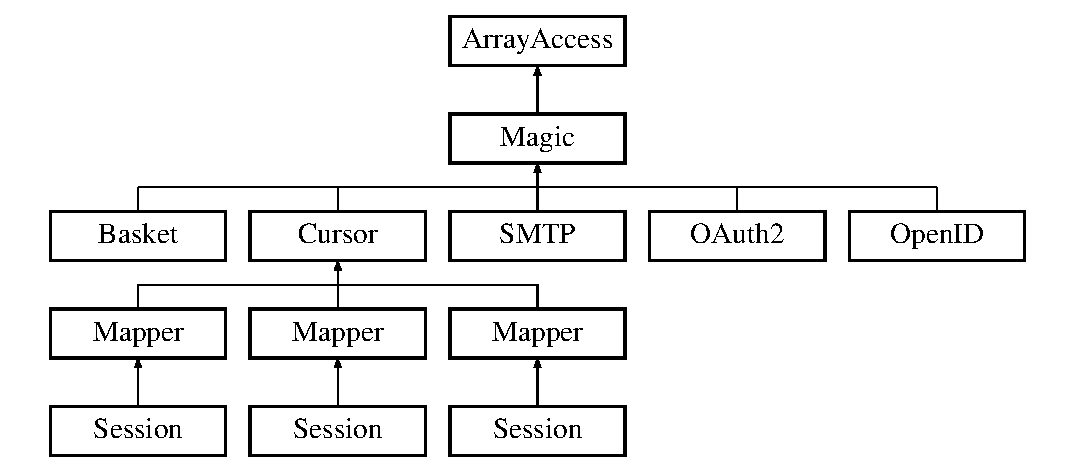
\includegraphics[height=5.000000cm]{class_magic}
\end{center}
\end{figure}
\subsection*{Public Member Functions}
\begin{DoxyCompactItemize}
\item 
\hyperlink{class_magic_ace1ae5be37bf26c172cc7ea4e1a65e26}{exists} (\$key)
\item 
\hyperlink{class_magic_ac8d8012023e560c81f55a629022cb65a}{set} (\$key, \$val)
\item 
\& \hyperlink{class_magic_ac3695923790b06917410e205068b8376}{get} (\$key)
\item 
\hyperlink{class_magic_a10a949ef75de6c82c98ac555f371ba83}{clear} (\$key)
\item 
\hyperlink{class_magic_a16da5af940f99a0df550a7f7c7c5d4e4}{offsetexists} (\$key)
\item 
\hyperlink{class_magic_a67693a9cff0abdfbbd353c36c00fb8d3}{offsetset} (\$key, \$val)
\item 
\& \hyperlink{class_magic_a4736f7355697c49bcd06b643b4077e8a}{offsetget} (\$key)
\item 
\hyperlink{class_magic_a414cd1cb3c09fc06e5e83502f6309dde}{offsetunset} (\$key)
\item 
\hyperlink{class_magic_ae858fed7cd2822fbceac154138b68baa}{\+\_\+\+\_\+isset} (\$key)
\item 
\hyperlink{class_magic_ae5e0d9ea041c1957ef04189b0b29657c}{\+\_\+\+\_\+set} (\$key, \$val)
\item 
\& \hyperlink{class_magic_ae23a2c24bd42a7be642cdb71b58dbc5a}{\+\_\+\+\_\+get} (\$key)
\item 
\hyperlink{class_magic_a41af7dd29c879b4c30978876ebdf4ba7}{\+\_\+\+\_\+unset} (\$key)
\end{DoxyCompactItemize}


\subsection{Detailed Description}
P\+HP magic wrapper. 

Definition at line 24 of file magic.\+php.



\subsection{Member Function Documentation}
\hypertarget{class_magic_ae23a2c24bd42a7be642cdb71b58dbc5a}{}\label{class_magic_ae23a2c24bd42a7be642cdb71b58dbc5a} 
\index{Magic@{Magic}!\+\_\+\+\_\+get@{\+\_\+\+\_\+get}}
\index{\+\_\+\+\_\+get@{\+\_\+\+\_\+get}!Magic@{Magic}}
\subsubsection{\texorpdfstring{\+\_\+\+\_\+get()}{\_\_get()}}
{\footnotesize\ttfamily \& \+\_\+\+\_\+get (\begin{DoxyParamCaption}\item[{}]{\$key }\end{DoxyParamCaption})}

Alias for \hyperlink{class_magic_a4736f7355697c49bcd06b643b4077e8a}{offsetget()} \begin{DoxyReturn}{Returns}
mixed 
\end{DoxyReturn}

\begin{DoxyParams}{Parameters}
{\em \$key} & string \\
\hline
\end{DoxyParams}


Definition at line 125 of file magic.\+php.

\hypertarget{class_magic_ae858fed7cd2822fbceac154138b68baa}{}\label{class_magic_ae858fed7cd2822fbceac154138b68baa} 
\index{Magic@{Magic}!\+\_\+\+\_\+isset@{\+\_\+\+\_\+isset}}
\index{\+\_\+\+\_\+isset@{\+\_\+\+\_\+isset}!Magic@{Magic}}
\subsubsection{\texorpdfstring{\+\_\+\+\_\+isset()}{\_\_isset()}}
{\footnotesize\ttfamily \+\_\+\+\_\+isset (\begin{DoxyParamCaption}\item[{}]{\$key }\end{DoxyParamCaption})}

Alias for \hyperlink{class_magic_a16da5af940f99a0df550a7f7c7c5d4e4}{offsetexists()} \begin{DoxyReturn}{Returns}
mixed 
\end{DoxyReturn}

\begin{DoxyParams}{Parameters}
{\em \$key} & string \\
\hline
\end{DoxyParams}


Definition at line 106 of file magic.\+php.

\hypertarget{class_magic_ae5e0d9ea041c1957ef04189b0b29657c}{}\label{class_magic_ae5e0d9ea041c1957ef04189b0b29657c} 
\index{Magic@{Magic}!\+\_\+\+\_\+set@{\+\_\+\+\_\+set}}
\index{\+\_\+\+\_\+set@{\+\_\+\+\_\+set}!Magic@{Magic}}
\subsubsection{\texorpdfstring{\+\_\+\+\_\+set()}{\_\_set()}}
{\footnotesize\ttfamily \+\_\+\+\_\+set (\begin{DoxyParamCaption}\item[{}]{\$key,  }\item[{}]{\$val }\end{DoxyParamCaption})}

Alias for \hyperlink{class_magic_a67693a9cff0abdfbbd353c36c00fb8d3}{offsetset()} \begin{DoxyReturn}{Returns}
mixed 
\end{DoxyReturn}

\begin{DoxyParams}{Parameters}
{\em \$key} & string \\
\hline
{\em \$val} & scalar \\
\hline
\end{DoxyParams}


Definition at line 116 of file magic.\+php.

\hypertarget{class_magic_a41af7dd29c879b4c30978876ebdf4ba7}{}\label{class_magic_a41af7dd29c879b4c30978876ebdf4ba7} 
\index{Magic@{Magic}!\+\_\+\+\_\+unset@{\+\_\+\+\_\+unset}}
\index{\+\_\+\+\_\+unset@{\+\_\+\+\_\+unset}!Magic@{Magic}}
\subsubsection{\texorpdfstring{\+\_\+\+\_\+unset()}{\_\_unset()}}
{\footnotesize\ttfamily \+\_\+\+\_\+unset (\begin{DoxyParamCaption}\item[{}]{\$key }\end{DoxyParamCaption})}

Alias for \hyperlink{class_magic_a414cd1cb3c09fc06e5e83502f6309dde}{offsetunset()} \begin{DoxyReturn}{Returns}
N\+U\+LL 
\end{DoxyReturn}

\begin{DoxyParams}{Parameters}
{\em \$key} & string \\
\hline
\end{DoxyParams}


Definition at line 135 of file magic.\+php.

\hypertarget{class_magic_a10a949ef75de6c82c98ac555f371ba83}{}\label{class_magic_a10a949ef75de6c82c98ac555f371ba83} 
\index{Magic@{Magic}!clear@{clear}}
\index{clear@{clear}!Magic@{Magic}}
\subsubsection{\texorpdfstring{clear()}{clear()}}
{\footnotesize\ttfamily clear (\begin{DoxyParamCaption}\item[{}]{\$key }\end{DoxyParamCaption})\hspace{0.3cm}{\ttfamily [abstract]}}

Unset key \begin{DoxyReturn}{Returns}
N\+U\+LL 
\end{DoxyReturn}

\begin{DoxyParams}{Parameters}
{\em \$key} & string \\
\hline
\end{DoxyParams}
\hypertarget{class_magic_ace1ae5be37bf26c172cc7ea4e1a65e26}{}\label{class_magic_ace1ae5be37bf26c172cc7ea4e1a65e26} 
\index{Magic@{Magic}!exists@{exists}}
\index{exists@{exists}!Magic@{Magic}}
\subsubsection{\texorpdfstring{exists()}{exists()}}
{\footnotesize\ttfamily exists (\begin{DoxyParamCaption}\item[{}]{\$key }\end{DoxyParamCaption})\hspace{0.3cm}{\ttfamily [abstract]}}

Return T\+R\+UE if key is not empty \begin{DoxyReturn}{Returns}
bool 
\end{DoxyReturn}

\begin{DoxyParams}{Parameters}
{\em \$key} & string \\
\hline
\end{DoxyParams}
\hypertarget{class_magic_ac3695923790b06917410e205068b8376}{}\label{class_magic_ac3695923790b06917410e205068b8376} 
\index{Magic@{Magic}!get@{get}}
\index{get@{get}!Magic@{Magic}}
\subsubsection{\texorpdfstring{get()}{get()}}
{\footnotesize\ttfamily \& get (\begin{DoxyParamCaption}\item[{}]{\$key }\end{DoxyParamCaption})\hspace{0.3cm}{\ttfamily [abstract]}}

Retrieve contents of key \begin{DoxyReturn}{Returns}
mixed 
\end{DoxyReturn}

\begin{DoxyParams}{Parameters}
{\em \$key} & string \\
\hline
\end{DoxyParams}
\hypertarget{class_magic_a16da5af940f99a0df550a7f7c7c5d4e4}{}\label{class_magic_a16da5af940f99a0df550a7f7c7c5d4e4} 
\index{Magic@{Magic}!offsetexists@{offsetexists}}
\index{offsetexists@{offsetexists}!Magic@{Magic}}
\subsubsection{\texorpdfstring{offsetexists()}{offsetexists()}}
{\footnotesize\ttfamily offsetexists (\begin{DoxyParamCaption}\item[{}]{\$key }\end{DoxyParamCaption})}

Convenience method for checking property value \begin{DoxyReturn}{Returns}
mixed 
\end{DoxyReturn}

\begin{DoxyParams}{Parameters}
{\em \$key} & string \\
\hline
\end{DoxyParams}


Definition at line 60 of file magic.\+php.

\hypertarget{class_magic_a4736f7355697c49bcd06b643b4077e8a}{}\label{class_magic_a4736f7355697c49bcd06b643b4077e8a} 
\index{Magic@{Magic}!offsetget@{offsetget}}
\index{offsetget@{offsetget}!Magic@{Magic}}
\subsubsection{\texorpdfstring{offsetget()}{offsetget()}}
{\footnotesize\ttfamily \& offsetget (\begin{DoxyParamCaption}\item[{}]{\$key }\end{DoxyParamCaption})}

Convenience method for retrieving property value \begin{DoxyReturn}{Returns}
mixed 
\end{DoxyReturn}

\begin{DoxyParams}{Parameters}
{\em \$key} & string \\
\hline
\end{DoxyParams}


Definition at line 81 of file magic.\+php.

\hypertarget{class_magic_a67693a9cff0abdfbbd353c36c00fb8d3}{}\label{class_magic_a67693a9cff0abdfbbd353c36c00fb8d3} 
\index{Magic@{Magic}!offsetset@{offsetset}}
\index{offsetset@{offsetset}!Magic@{Magic}}
\subsubsection{\texorpdfstring{offsetset()}{offsetset()}}
{\footnotesize\ttfamily offsetset (\begin{DoxyParamCaption}\item[{}]{\$key,  }\item[{}]{\$val }\end{DoxyParamCaption})}

Convenience method for assigning property value \begin{DoxyReturn}{Returns}
mixed 
\end{DoxyReturn}

\begin{DoxyParams}{Parameters}
{\em \$key} & string \\
\hline
{\em \$val} & scalar \\
\hline
\end{DoxyParams}


Definition at line 71 of file magic.\+php.

\hypertarget{class_magic_a414cd1cb3c09fc06e5e83502f6309dde}{}\label{class_magic_a414cd1cb3c09fc06e5e83502f6309dde} 
\index{Magic@{Magic}!offsetunset@{offsetunset}}
\index{offsetunset@{offsetunset}!Magic@{Magic}}
\subsubsection{\texorpdfstring{offsetunset()}{offsetunset()}}
{\footnotesize\ttfamily offsetunset (\begin{DoxyParamCaption}\item[{}]{\$key }\end{DoxyParamCaption})}

Convenience method for removing property value \begin{DoxyReturn}{Returns}
N\+U\+LL 
\end{DoxyReturn}

\begin{DoxyParams}{Parameters}
{\em \$key} & string \\
\hline
\end{DoxyParams}


Definition at line 94 of file magic.\+php.

\hypertarget{class_magic_ac8d8012023e560c81f55a629022cb65a}{}\label{class_magic_ac8d8012023e560c81f55a629022cb65a} 
\index{Magic@{Magic}!set@{set}}
\index{set@{set}!Magic@{Magic}}
\subsubsection{\texorpdfstring{set()}{set()}}
{\footnotesize\ttfamily set (\begin{DoxyParamCaption}\item[{}]{\$key,  }\item[{}]{\$val }\end{DoxyParamCaption})\hspace{0.3cm}{\ttfamily [abstract]}}

Bind value to key \begin{DoxyReturn}{Returns}
mixed 
\end{DoxyReturn}

\begin{DoxyParams}{Parameters}
{\em \$key} & string \\
\hline
{\em \$val} & mixed \\
\hline
\end{DoxyParams}


The documentation for this class was generated from the following file\+:\begin{DoxyCompactItemize}
\item 
/\+Users/aplennevaux/\+G\+I\+T\+H\+U\+B/\+Visionary-\/website/src/vendor/bcosca/fatfree/lib/magic.\+php\end{DoxyCompactItemize}

\hypertarget{class_d_b_1_1_mongo_1_1_mapper}{}\section{Mapper Class Reference}
\label{class_d_b_1_1_mongo_1_1_mapper}\index{Mapper@{Mapper}}


Mongo\+DB mapper.  


Inheritance diagram for Mapper\+:\begin{figure}[H]
\begin{center}
\leavevmode
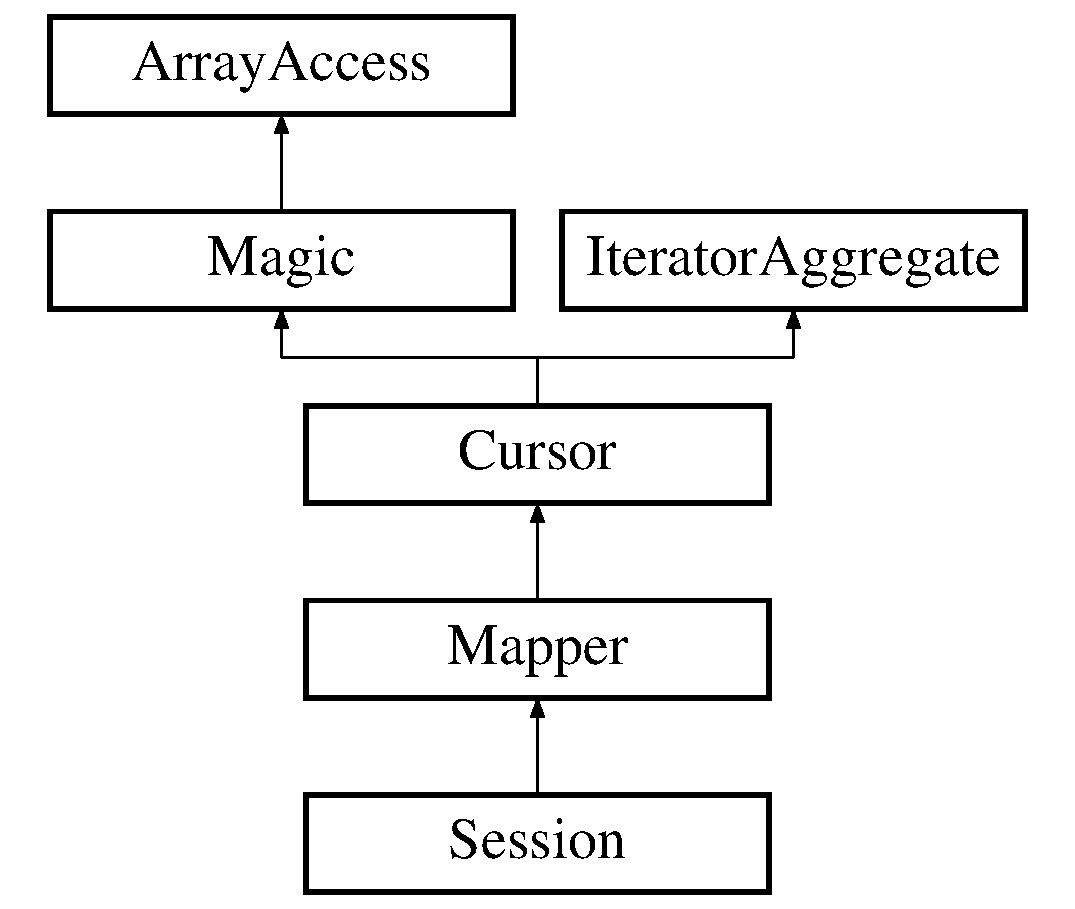
\includegraphics[height=5.000000cm]{class_d_b_1_1_mongo_1_1_mapper}
\end{center}
\end{figure}
\subsection*{Public Member Functions}
\begin{DoxyCompactItemize}
\item 
\hyperlink{class_d_b_1_1_mongo_1_1_mapper_a38948c2fb1711f49b72f123cbd91e611}{dbtype} ()
\item 
\hyperlink{class_d_b_1_1_mongo_1_1_mapper_ace1ae5be37bf26c172cc7ea4e1a65e26}{exists} (\$key)
\item 
\hyperlink{class_d_b_1_1_mongo_1_1_mapper_ac8d8012023e560c81f55a629022cb65a}{set} (\$key, \$val)
\item 
\& \hyperlink{class_d_b_1_1_mongo_1_1_mapper_ac3695923790b06917410e205068b8376}{get} (\$key)
\item 
\hyperlink{class_d_b_1_1_mongo_1_1_mapper_a10a949ef75de6c82c98ac555f371ba83}{clear} (\$key)
\item 
\hyperlink{class_d_b_1_1_mongo_1_1_mapper_aa33294a722f17e6e4946223bb73f13ab}{cast} (\$obj=N\+U\+LL)
\item 
\hyperlink{class_d_b_1_1_mongo_1_1_mapper_a57aa9e27404419f6796e017c7251aad4}{select} (\$\hyperlink{class_d_b_1_1_mongo_1_1_mapper_a9dfc1601eaf8348bed6ba5622f725971}{fields}=N\+U\+LL, \$filter=N\+U\+LL, array \$options=N\+U\+LL, \$ttl=0)
\item 
\hyperlink{class_d_b_1_1_mongo_1_1_mapper_a45e70f55799839fc0286bc94000924a7}{find} (\$filter=N\+U\+LL, array \$options=N\+U\+LL, \$ttl=0)
\item 
\hyperlink{class_d_b_1_1_mongo_1_1_mapper_ab1f3a3bd85dca49dceaea57f2fe21abf}{count} (\$filter=N\+U\+LL, \$ttl=0)
\item 
\hyperlink{class_d_b_1_1_mongo_1_1_mapper_aad399d205074eaeed711d5e0157b3c0a}{skip} (\$ofs=1)
\item 
\hyperlink{class_d_b_1_1_mongo_1_1_mapper_a473241246338cfccc4709ba896749019}{insert} ()
\item 
\hyperlink{class_d_b_1_1_mongo_1_1_mapper_a842e4774e3b3601a005b995c02f7e883}{update} ()
\item 
\hyperlink{class_d_b_1_1_mongo_1_1_mapper_aa7210074cfc1eda78dc492d8b8a96616}{erase} (\$filter=N\+U\+LL)
\item 
\hyperlink{class_d_b_1_1_mongo_1_1_mapper_a4a20559544fdf4dcb457e258dc976cf8}{reset} ()
\item 
\hyperlink{class_d_b_1_1_mongo_1_1_mapper_adffe904ab38af888d9b033647ec6d935}{copyfrom} (\$var, \$func=N\+U\+LL)
\item 
\hyperlink{class_d_b_1_1_mongo_1_1_mapper_a4bcf54f913758fb093c35ea81fc29615}{copyto} (\$key)
\item 
\hyperlink{class_d_b_1_1_mongo_1_1_mapper_a9dfc1601eaf8348bed6ba5622f725971}{fields} ()
\item 
\hyperlink{class_d_b_1_1_mongo_1_1_mapper_aa3b267270ebe136571604fe35ce404fa}{cursor} ()
\item 
\hyperlink{class_d_b_1_1_mongo_1_1_mapper_a7f835c25df4cb49d02328644722656da}{getiterator} ()
\item 
\hyperlink{class_d_b_1_1_mongo_1_1_mapper_aebc412b4073d1b6a2439a70a2bbaac47}{\+\_\+\+\_\+construct} (\textbackslash{}\hyperlink{class_d_b_1_1_mongo}{D\+B\textbackslash{}\+Mongo} \$db, \$collection, \$\hyperlink{class_d_b_1_1_mongo_1_1_mapper_a9dfc1601eaf8348bed6ba5622f725971}{fields}=N\+U\+LL)
\end{DoxyCompactItemize}
\subsection*{Data Fields}
\begin{DoxyCompactItemize}
\item 
\hypertarget{class_d_b_1_1_mongo_1_1_mapper_ab9e21dbbe588414048003c715034e2aa}{}\label{class_d_b_1_1_mongo_1_1_mapper_ab9e21dbbe588414048003c715034e2aa} 
\hyperlink{class_d_b_1_1_mongo_1_1_mapper_ab9e21dbbe588414048003c715034e2aa}{\$collection}
\begin{DoxyCompactList}\small\item\em \hyperlink{class_d_b_1_1_mongo}{Mongo} collection. \end{DoxyCompactList}\item 
\hypertarget{class_d_b_1_1_mongo_1_1_mapper_ac5a31edb787609a3143dec9bfa8063ea}{}\label{class_d_b_1_1_mongo_1_1_mapper_ac5a31edb787609a3143dec9bfa8063ea} 
\hyperlink{class_d_b_1_1_mongo_1_1_mapper_ac5a31edb787609a3143dec9bfa8063ea}{\$document} =\mbox{[}$\,$\mbox{]}
\begin{DoxyCompactList}\small\item\em \hyperlink{class_d_b_1_1_mongo}{Mongo} document. \end{DoxyCompactList}\item 
\hypertarget{class_d_b_1_1_mongo_1_1_mapper_a256b6d58b346bcd39d5bf5d49de70df2}{}\label{class_d_b_1_1_mongo_1_1_mapper_a256b6d58b346bcd39d5bf5d49de70df2} 
\hyperlink{class_d_b_1_1_mongo_1_1_mapper_a256b6d58b346bcd39d5bf5d49de70df2}{\$cursor}
\begin{DoxyCompactList}\small\item\em \hyperlink{class_d_b_1_1_mongo}{Mongo} cursor. \end{DoxyCompactList}\item 
\hypertarget{class_d_b_1_1_mongo_1_1_mapper_ab2303c817e3b402b77b7f99627b9c319}{}\label{class_d_b_1_1_mongo_1_1_mapper_ab2303c817e3b402b77b7f99627b9c319} 
\hyperlink{class_d_b_1_1_mongo_1_1_mapper_ab2303c817e3b402b77b7f99627b9c319}{\$fields}
\begin{DoxyCompactList}\small\item\em Defined fields. \end{DoxyCompactList}\end{DoxyCompactItemize}
\subsection*{Protected Member Functions}
\begin{DoxyCompactItemize}
\item 
\hyperlink{class_d_b_1_1_mongo_1_1_mapper_a60e4b1320f31f4049ad7867bd739c14d}{factory} (\$row)
\end{DoxyCompactItemize}
\subsection*{Protected Attributes}
\begin{DoxyCompactItemize}
\item 
\hypertarget{class_d_b_1_1_mongo_1_1_mapper_a1fa3127fc82f96b1436d871ef02be319}{}\label{class_d_b_1_1_mongo_1_1_mapper_a1fa3127fc82f96b1436d871ef02be319} 
\hyperlink{class_d_b_1_1_mongo_1_1_mapper_a1fa3127fc82f96b1436d871ef02be319}{\$db}
\begin{DoxyCompactList}\small\item\em Mongo\+DB wrapper. \end{DoxyCompactList}\end{DoxyCompactItemize}


\subsection{Detailed Description}
Mongo\+DB mapper. 

Definition at line 26 of file mapper.\+php.



\subsection{Constructor \& Destructor Documentation}
\hypertarget{class_d_b_1_1_mongo_1_1_mapper_aebc412b4073d1b6a2439a70a2bbaac47}{}\label{class_d_b_1_1_mongo_1_1_mapper_aebc412b4073d1b6a2439a70a2bbaac47} 
\index{D\+B\+::\+Mongo\+::\+Mapper@{D\+B\+::\+Mongo\+::\+Mapper}!\+\_\+\+\_\+construct@{\+\_\+\+\_\+construct}}
\index{\+\_\+\+\_\+construct@{\+\_\+\+\_\+construct}!D\+B\+::\+Mongo\+::\+Mapper@{D\+B\+::\+Mongo\+::\+Mapper}}
\subsubsection{\texorpdfstring{\+\_\+\+\_\+construct()}{\_\_construct()}}
{\footnotesize\ttfamily \+\_\+\+\_\+construct (\begin{DoxyParamCaption}\item[{\textbackslash{}\hyperlink{class_d_b_1_1_mongo}{D\+B\textbackslash{}\+Mongo}}]{\$db,  }\item[{}]{\$collection,  }\item[{}]{\$fields = {\ttfamily NULL} }\end{DoxyParamCaption})}

Instantiate class \begin{DoxyReturn}{Returns}
void 
\end{DoxyReturn}

\begin{DoxyParams}{Parameters}
{\em \$db} & object \\
\hline
{\em \$collection} & string \\
\hline
{\em \$fields} & array \\
\hline
\end{DoxyParams}


Definition at line 358 of file mapper.\+php.



\subsection{Member Function Documentation}
\hypertarget{class_d_b_1_1_mongo_1_1_mapper_aa33294a722f17e6e4946223bb73f13ab}{}\label{class_d_b_1_1_mongo_1_1_mapper_aa33294a722f17e6e4946223bb73f13ab} 
\index{D\+B\+::\+Mongo\+::\+Mapper@{D\+B\+::\+Mongo\+::\+Mapper}!cast@{cast}}
\index{cast@{cast}!D\+B\+::\+Mongo\+::\+Mapper@{D\+B\+::\+Mongo\+::\+Mapper}}
\subsubsection{\texorpdfstring{cast()}{cast()}}
{\footnotesize\ttfamily cast (\begin{DoxyParamCaption}\item[{}]{\$obj = {\ttfamily NULL} }\end{DoxyParamCaption})}

Return fields of mapper object as an associative array \begin{DoxyReturn}{Returns}
array 
\end{DoxyReturn}

\begin{DoxyParams}{Parameters}
{\em \$obj} & object \\
\hline
\end{DoxyParams}


Definition at line 108 of file mapper.\+php.

\hypertarget{class_d_b_1_1_mongo_1_1_mapper_a10a949ef75de6c82c98ac555f371ba83}{}\label{class_d_b_1_1_mongo_1_1_mapper_a10a949ef75de6c82c98ac555f371ba83} 
\index{D\+B\+::\+Mongo\+::\+Mapper@{D\+B\+::\+Mongo\+::\+Mapper}!clear@{clear}}
\index{clear@{clear}!D\+B\+::\+Mongo\+::\+Mapper@{D\+B\+::\+Mongo\+::\+Mapper}}
\subsubsection{\texorpdfstring{clear()}{clear()}}
{\footnotesize\ttfamily clear (\begin{DoxyParamCaption}\item[{}]{\$key }\end{DoxyParamCaption})}

Delete field \begin{DoxyReturn}{Returns}
N\+U\+LL 
\end{DoxyReturn}

\begin{DoxyParams}{Parameters}
{\em \$key} & string \\
\hline
\end{DoxyParams}


Definition at line 83 of file mapper.\+php.

\hypertarget{class_d_b_1_1_mongo_1_1_mapper_adffe904ab38af888d9b033647ec6d935}{}\label{class_d_b_1_1_mongo_1_1_mapper_adffe904ab38af888d9b033647ec6d935} 
\index{D\+B\+::\+Mongo\+::\+Mapper@{D\+B\+::\+Mongo\+::\+Mapper}!copyfrom@{copyfrom}}
\index{copyfrom@{copyfrom}!D\+B\+::\+Mongo\+::\+Mapper@{D\+B\+::\+Mongo\+::\+Mapper}}
\subsubsection{\texorpdfstring{copyfrom()}{copyfrom()}}
{\footnotesize\ttfamily copyfrom (\begin{DoxyParamCaption}\item[{}]{\$var,  }\item[{}]{\$func = {\ttfamily NULL} }\end{DoxyParamCaption})}

Hydrate mapper object using hive array variable \begin{DoxyReturn}{Returns}
N\+U\+LL 
\end{DoxyReturn}

\begin{DoxyParams}{Parameters}
{\em \$var} & array$\vert$string \\
\hline
{\em \$func} & callback \\
\hline
\end{DoxyParams}


Definition at line 307 of file mapper.\+php.

\hypertarget{class_d_b_1_1_mongo_1_1_mapper_a4bcf54f913758fb093c35ea81fc29615}{}\label{class_d_b_1_1_mongo_1_1_mapper_a4bcf54f913758fb093c35ea81fc29615} 
\index{D\+B\+::\+Mongo\+::\+Mapper@{D\+B\+::\+Mongo\+::\+Mapper}!copyto@{copyto}}
\index{copyto@{copyto}!D\+B\+::\+Mongo\+::\+Mapper@{D\+B\+::\+Mongo\+::\+Mapper}}
\subsubsection{\texorpdfstring{copyto()}{copyto()}}
{\footnotesize\ttfamily copyto (\begin{DoxyParamCaption}\item[{}]{\$key }\end{DoxyParamCaption})}

Populate hive array variable with mapper fields \begin{DoxyReturn}{Returns}
N\+U\+LL 
\end{DoxyReturn}

\begin{DoxyParams}{Parameters}
{\em \$key} & string \\
\hline
\end{DoxyParams}


Definition at line 321 of file mapper.\+php.

\hypertarget{class_d_b_1_1_mongo_1_1_mapper_ab1f3a3bd85dca49dceaea57f2fe21abf}{}\label{class_d_b_1_1_mongo_1_1_mapper_ab1f3a3bd85dca49dceaea57f2fe21abf} 
\index{D\+B\+::\+Mongo\+::\+Mapper@{D\+B\+::\+Mongo\+::\+Mapper}!count@{count}}
\index{count@{count}!D\+B\+::\+Mongo\+::\+Mapper@{D\+B\+::\+Mongo\+::\+Mapper}}
\subsubsection{\texorpdfstring{count()}{count()}}
{\footnotesize\ttfamily count (\begin{DoxyParamCaption}\item[{}]{\$filter = {\ttfamily NULL},  }\item[{}]{\$ttl = {\ttfamily 0} }\end{DoxyParamCaption})}

Count records that match criteria \begin{DoxyReturn}{Returns}
int 
\end{DoxyReturn}

\begin{DoxyParams}{Parameters}
{\em \$filter} & array \\
\hline
{\em \$ttl} & int \\
\hline
\end{DoxyParams}


Definition at line 205 of file mapper.\+php.

\hypertarget{class_d_b_1_1_mongo_1_1_mapper_aa3b267270ebe136571604fe35ce404fa}{}\label{class_d_b_1_1_mongo_1_1_mapper_aa3b267270ebe136571604fe35ce404fa} 
\index{D\+B\+::\+Mongo\+::\+Mapper@{D\+B\+::\+Mongo\+::\+Mapper}!cursor@{cursor}}
\index{cursor@{cursor}!D\+B\+::\+Mongo\+::\+Mapper@{D\+B\+::\+Mongo\+::\+Mapper}}
\subsubsection{\texorpdfstring{cursor()}{cursor()}}
{\footnotesize\ttfamily cursor (\begin{DoxyParamCaption}{ }\end{DoxyParamCaption})}

Return the cursor from last query \begin{DoxyReturn}{Returns}
object$\vert$\+N\+U\+LL 
\end{DoxyReturn}


Definition at line 339 of file mapper.\+php.

\hypertarget{class_d_b_1_1_mongo_1_1_mapper_a38948c2fb1711f49b72f123cbd91e611}{}\label{class_d_b_1_1_mongo_1_1_mapper_a38948c2fb1711f49b72f123cbd91e611} 
\index{D\+B\+::\+Mongo\+::\+Mapper@{D\+B\+::\+Mongo\+::\+Mapper}!dbtype@{dbtype}}
\index{dbtype@{dbtype}!D\+B\+::\+Mongo\+::\+Mapper@{D\+B\+::\+Mongo\+::\+Mapper}}
\subsubsection{\texorpdfstring{dbtype()}{dbtype()}}
{\footnotesize\ttfamily dbtype (\begin{DoxyParamCaption}{ }\end{DoxyParamCaption})}

Return database type \begin{DoxyReturn}{Returns}
string 
\end{DoxyReturn}


Definition at line 44 of file mapper.\+php.

\hypertarget{class_d_b_1_1_mongo_1_1_mapper_aa7210074cfc1eda78dc492d8b8a96616}{}\label{class_d_b_1_1_mongo_1_1_mapper_aa7210074cfc1eda78dc492d8b8a96616} 
\index{D\+B\+::\+Mongo\+::\+Mapper@{D\+B\+::\+Mongo\+::\+Mapper}!erase@{erase}}
\index{erase@{erase}!D\+B\+::\+Mongo\+::\+Mapper@{D\+B\+::\+Mongo\+::\+Mapper}}
\subsubsection{\texorpdfstring{erase()}{erase()}}
{\footnotesize\ttfamily erase (\begin{DoxyParamCaption}\item[{}]{\$filter = {\ttfamily NULL} }\end{DoxyParamCaption})}

Delete current record \begin{DoxyReturn}{Returns}
bool 
\end{DoxyReturn}

\begin{DoxyParams}{Parameters}
{\em \$filter} & array \\
\hline
\end{DoxyParams}


Definition at line 275 of file mapper.\+php.

\hypertarget{class_d_b_1_1_mongo_1_1_mapper_ace1ae5be37bf26c172cc7ea4e1a65e26}{}\label{class_d_b_1_1_mongo_1_1_mapper_ace1ae5be37bf26c172cc7ea4e1a65e26} 
\index{D\+B\+::\+Mongo\+::\+Mapper@{D\+B\+::\+Mongo\+::\+Mapper}!exists@{exists}}
\index{exists@{exists}!D\+B\+::\+Mongo\+::\+Mapper@{D\+B\+::\+Mongo\+::\+Mapper}}
\subsubsection{\texorpdfstring{exists()}{exists()}}
{\footnotesize\ttfamily exists (\begin{DoxyParamCaption}\item[{}]{\$key }\end{DoxyParamCaption})}

Return T\+R\+UE if field is defined \begin{DoxyReturn}{Returns}
bool 
\end{DoxyReturn}

\begin{DoxyParams}{Parameters}
{\em \$key} & string \\
\hline
\end{DoxyParams}


Definition at line 53 of file mapper.\+php.

\hypertarget{class_d_b_1_1_mongo_1_1_mapper_a60e4b1320f31f4049ad7867bd739c14d}{}\label{class_d_b_1_1_mongo_1_1_mapper_a60e4b1320f31f4049ad7867bd739c14d} 
\index{D\+B\+::\+Mongo\+::\+Mapper@{D\+B\+::\+Mongo\+::\+Mapper}!factory@{factory}}
\index{factory@{factory}!D\+B\+::\+Mongo\+::\+Mapper@{D\+B\+::\+Mongo\+::\+Mapper}}
\subsubsection{\texorpdfstring{factory()}{factory()}}
{\footnotesize\ttfamily factory (\begin{DoxyParamCaption}\item[{}]{\$row }\end{DoxyParamCaption})\hspace{0.3cm}{\ttfamily [protected]}}

Convert array to mapper object \begin{DoxyReturn}{Returns}
static 
\end{DoxyReturn}

\begin{DoxyParams}{Parameters}
{\em \$row} & array \\
\hline
\end{DoxyParams}


Definition at line 92 of file mapper.\+php.

\hypertarget{class_d_b_1_1_mongo_1_1_mapper_a9dfc1601eaf8348bed6ba5622f725971}{}\label{class_d_b_1_1_mongo_1_1_mapper_a9dfc1601eaf8348bed6ba5622f725971} 
\index{D\+B\+::\+Mongo\+::\+Mapper@{D\+B\+::\+Mongo\+::\+Mapper}!fields@{fields}}
\index{fields@{fields}!D\+B\+::\+Mongo\+::\+Mapper@{D\+B\+::\+Mongo\+::\+Mapper}}
\subsubsection{\texorpdfstring{fields()}{fields()}}
{\footnotesize\ttfamily fields (\begin{DoxyParamCaption}{ }\end{DoxyParamCaption})}

Return field names \begin{DoxyReturn}{Returns}
array 
\end{DoxyReturn}


Definition at line 331 of file mapper.\+php.

\hypertarget{class_d_b_1_1_mongo_1_1_mapper_a45e70f55799839fc0286bc94000924a7}{}\label{class_d_b_1_1_mongo_1_1_mapper_a45e70f55799839fc0286bc94000924a7} 
\index{D\+B\+::\+Mongo\+::\+Mapper@{D\+B\+::\+Mongo\+::\+Mapper}!find@{find}}
\index{find@{find}!D\+B\+::\+Mongo\+::\+Mapper@{D\+B\+::\+Mongo\+::\+Mapper}}
\subsubsection{\texorpdfstring{find()}{find()}}
{\footnotesize\ttfamily find (\begin{DoxyParamCaption}\item[{}]{\$filter = {\ttfamily NULL},  }\item[{array}]{\$options = {\ttfamily NULL},  }\item[{}]{\$ttl = {\ttfamily 0} }\end{DoxyParamCaption})}

Return records that match criteria \begin{DoxyReturn}{Returns}
static\mbox{[}\mbox{]} 
\end{DoxyReturn}

\begin{DoxyParams}{Parameters}
{\em \$filter} & array \\
\hline
{\em \$options} & array \\
\hline
{\em \$ttl} & int \\
\hline
\end{DoxyParams}


Definition at line 187 of file mapper.\+php.

\hypertarget{class_d_b_1_1_mongo_1_1_mapper_ac3695923790b06917410e205068b8376}{}\label{class_d_b_1_1_mongo_1_1_mapper_ac3695923790b06917410e205068b8376} 
\index{D\+B\+::\+Mongo\+::\+Mapper@{D\+B\+::\+Mongo\+::\+Mapper}!get@{get}}
\index{get@{get}!D\+B\+::\+Mongo\+::\+Mapper@{D\+B\+::\+Mongo\+::\+Mapper}}
\subsubsection{\texorpdfstring{get()}{get()}}
{\footnotesize\ttfamily \& get (\begin{DoxyParamCaption}\item[{}]{\$key }\end{DoxyParamCaption})}

Retrieve value of field \begin{DoxyReturn}{Returns}
scalar$\vert$\+F\+A\+L\+SE 
\end{DoxyReturn}

\begin{DoxyParams}{Parameters}
{\em \$key} & string \\
\hline
\end{DoxyParams}


Definition at line 72 of file mapper.\+php.

\hypertarget{class_d_b_1_1_mongo_1_1_mapper_a7f835c25df4cb49d02328644722656da}{}\label{class_d_b_1_1_mongo_1_1_mapper_a7f835c25df4cb49d02328644722656da} 
\index{D\+B\+::\+Mongo\+::\+Mapper@{D\+B\+::\+Mongo\+::\+Mapper}!getiterator@{getiterator}}
\index{getiterator@{getiterator}!D\+B\+::\+Mongo\+::\+Mapper@{D\+B\+::\+Mongo\+::\+Mapper}}
\subsubsection{\texorpdfstring{getiterator()}{getiterator()}}
{\footnotesize\ttfamily getiterator (\begin{DoxyParamCaption}{ }\end{DoxyParamCaption})}

Retrieve external iterator for fields \begin{DoxyReturn}{Returns}
object 
\end{DoxyReturn}


Definition at line 347 of file mapper.\+php.

\hypertarget{class_d_b_1_1_mongo_1_1_mapper_a473241246338cfccc4709ba896749019}{}\label{class_d_b_1_1_mongo_1_1_mapper_a473241246338cfccc4709ba896749019} 
\index{D\+B\+::\+Mongo\+::\+Mapper@{D\+B\+::\+Mongo\+::\+Mapper}!insert@{insert}}
\index{insert@{insert}!D\+B\+::\+Mongo\+::\+Mapper@{D\+B\+::\+Mongo\+::\+Mapper}}
\subsubsection{\texorpdfstring{insert()}{insert()}}
{\footnotesize\ttfamily insert (\begin{DoxyParamCaption}{ }\end{DoxyParamCaption})}

Insert new record \begin{DoxyReturn}{Returns}
array 
\end{DoxyReturn}


Definition at line 236 of file mapper.\+php.

\hypertarget{class_d_b_1_1_mongo_1_1_mapper_a4a20559544fdf4dcb457e258dc976cf8}{}\label{class_d_b_1_1_mongo_1_1_mapper_a4a20559544fdf4dcb457e258dc976cf8} 
\index{D\+B\+::\+Mongo\+::\+Mapper@{D\+B\+::\+Mongo\+::\+Mapper}!reset@{reset}}
\index{reset@{reset}!D\+B\+::\+Mongo\+::\+Mapper@{D\+B\+::\+Mongo\+::\+Mapper}}
\subsubsection{\texorpdfstring{reset()}{reset()}}
{\footnotesize\ttfamily reset (\begin{DoxyParamCaption}{ }\end{DoxyParamCaption})}

Reset cursor \begin{DoxyReturn}{Returns}
N\+U\+LL 
\end{DoxyReturn}


Definition at line 296 of file mapper.\+php.

\hypertarget{class_d_b_1_1_mongo_1_1_mapper_a57aa9e27404419f6796e017c7251aad4}{}\label{class_d_b_1_1_mongo_1_1_mapper_a57aa9e27404419f6796e017c7251aad4} 
\index{D\+B\+::\+Mongo\+::\+Mapper@{D\+B\+::\+Mongo\+::\+Mapper}!select@{select}}
\index{select@{select}!D\+B\+::\+Mongo\+::\+Mapper@{D\+B\+::\+Mongo\+::\+Mapper}}
\subsubsection{\texorpdfstring{select()}{select()}}
{\footnotesize\ttfamily select (\begin{DoxyParamCaption}\item[{}]{\$fields = {\ttfamily NULL},  }\item[{}]{\$filter = {\ttfamily NULL},  }\item[{array}]{\$options = {\ttfamily NULL},  }\item[{}]{\$ttl = {\ttfamily 0} }\end{DoxyParamCaption})}

Build query and execute \begin{DoxyReturn}{Returns}
static\mbox{[}\mbox{]} 
\end{DoxyReturn}

\begin{DoxyParams}{Parameters}
{\em \$fields} & string \\
\hline
{\em \$filter} & array \\
\hline
{\em \$options} & array \\
\hline
{\em \$ttl} & int \\
\hline
\end{DoxyParams}


Definition at line 122 of file mapper.\+php.

\hypertarget{class_d_b_1_1_mongo_1_1_mapper_ac8d8012023e560c81f55a629022cb65a}{}\label{class_d_b_1_1_mongo_1_1_mapper_ac8d8012023e560c81f55a629022cb65a} 
\index{D\+B\+::\+Mongo\+::\+Mapper@{D\+B\+::\+Mongo\+::\+Mapper}!set@{set}}
\index{set@{set}!D\+B\+::\+Mongo\+::\+Mapper@{D\+B\+::\+Mongo\+::\+Mapper}}
\subsubsection{\texorpdfstring{set()}{set()}}
{\footnotesize\ttfamily set (\begin{DoxyParamCaption}\item[{}]{\$key,  }\item[{}]{\$val }\end{DoxyParamCaption})}

Assign value to field \begin{DoxyReturn}{Returns}
scalar$\vert$\+F\+A\+L\+SE 
\end{DoxyReturn}

\begin{DoxyParams}{Parameters}
{\em \$key} & string \\
\hline
{\em \$val} & scalar \\
\hline
\end{DoxyParams}


Definition at line 63 of file mapper.\+php.

\hypertarget{class_d_b_1_1_mongo_1_1_mapper_aad399d205074eaeed711d5e0157b3c0a}{}\label{class_d_b_1_1_mongo_1_1_mapper_aad399d205074eaeed711d5e0157b3c0a} 
\index{D\+B\+::\+Mongo\+::\+Mapper@{D\+B\+::\+Mongo\+::\+Mapper}!skip@{skip}}
\index{skip@{skip}!D\+B\+::\+Mongo\+::\+Mapper@{D\+B\+::\+Mongo\+::\+Mapper}}
\subsubsection{\texorpdfstring{skip()}{skip()}}
{\footnotesize\ttfamily skip (\begin{DoxyParamCaption}\item[{}]{\$ofs = {\ttfamily 1} }\end{DoxyParamCaption})}

Return record at specified offset using criteria of previous \hyperlink{class_d_b_1_1_cursor_a4db66c122e6274a3d653eff639e8476f}{load()} call and make it active \begin{DoxyReturn}{Returns}
array 
\end{DoxyReturn}

\begin{DoxyParams}{Parameters}
{\em \$ofs} & int \\
\hline
\end{DoxyParams}


Definition at line 225 of file mapper.\+php.

\hypertarget{class_d_b_1_1_mongo_1_1_mapper_a842e4774e3b3601a005b995c02f7e883}{}\label{class_d_b_1_1_mongo_1_1_mapper_a842e4774e3b3601a005b995c02f7e883} 
\index{D\+B\+::\+Mongo\+::\+Mapper@{D\+B\+::\+Mongo\+::\+Mapper}!update@{update}}
\index{update@{update}!D\+B\+::\+Mongo\+::\+Mapper@{D\+B\+::\+Mongo\+::\+Mapper}}
\subsubsection{\texorpdfstring{update()}{update()}}
{\footnotesize\ttfamily update (\begin{DoxyParamCaption}{ }\end{DoxyParamCaption})}

Update current record \begin{DoxyReturn}{Returns}
array 
\end{DoxyReturn}


Definition at line 256 of file mapper.\+php.



The documentation for this class was generated from the following file\+:\begin{DoxyCompactItemize}
\item 
/\+Users/aplennevaux/\+G\+I\+T\+H\+U\+B/\+Visionary-\/website/src/vendor/bcosca/fatfree/lib/db/mongo/mapper.\+php\end{DoxyCompactItemize}

\hypertarget{class_d_b_1_1_s_q_l_1_1_mapper}{}\section{Mapper Class Reference}
\label{class_d_b_1_1_s_q_l_1_1_mapper}\index{Mapper@{Mapper}}


\hyperlink{class_d_b_1_1_s_q_l}{S\+QL} data mapper.  


Inheritance diagram for Mapper\+:\begin{figure}[H]
\begin{center}
\leavevmode
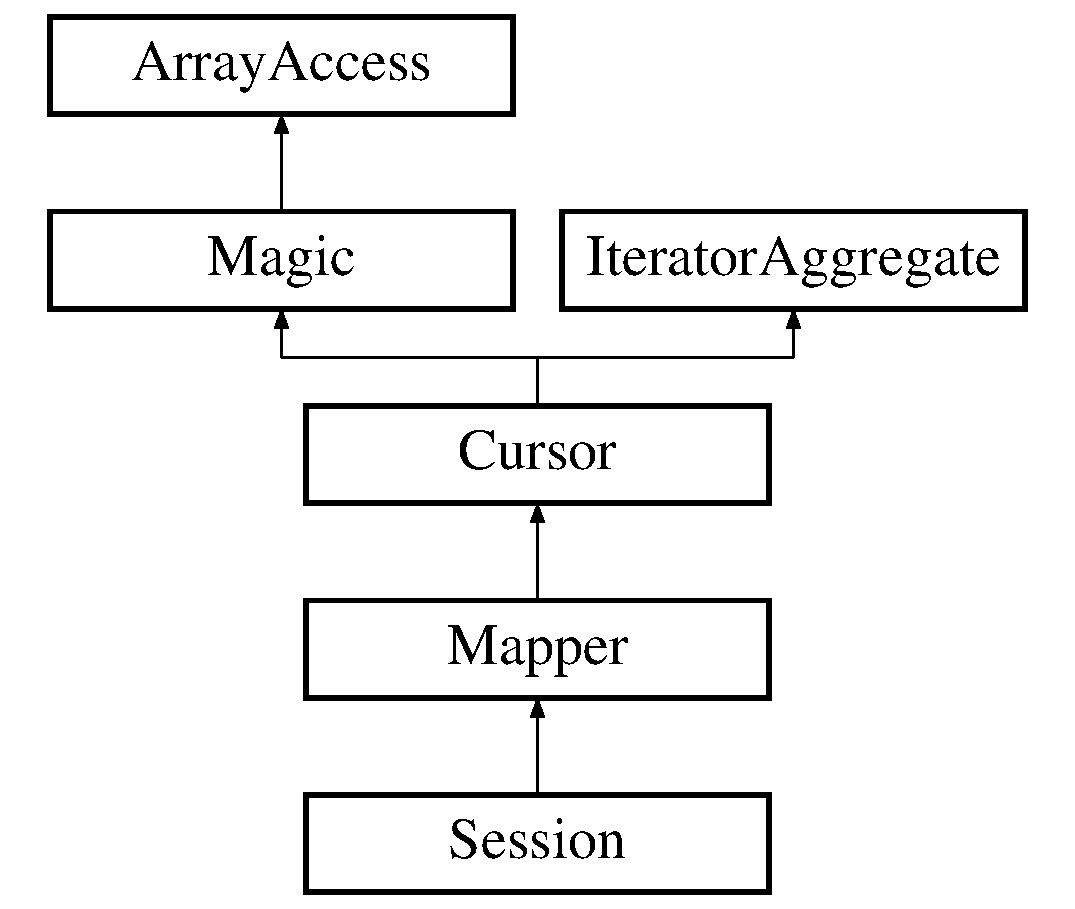
\includegraphics[height=5.000000cm]{class_d_b_1_1_s_q_l_1_1_mapper}
\end{center}
\end{figure}
\subsection*{Public Member Functions}
\begin{DoxyCompactItemize}
\item 
\hyperlink{class_d_b_1_1_s_q_l_1_1_mapper_a38948c2fb1711f49b72f123cbd91e611}{dbtype} ()
\item 
\hyperlink{class_d_b_1_1_s_q_l_1_1_mapper_a5aa7b43c8ec77df216a71a27da0a321c}{table} ()
\item 
\hyperlink{class_d_b_1_1_s_q_l_1_1_mapper_ace1ae5be37bf26c172cc7ea4e1a65e26}{exists} (\$key)
\item 
\hyperlink{class_d_b_1_1_s_q_l_1_1_mapper_a20f740dfb4d3aa525f4109bdcf41dab7}{changed} (\$key=N\+U\+LL)
\item 
\hyperlink{class_d_b_1_1_s_q_l_1_1_mapper_ac8d8012023e560c81f55a629022cb65a}{set} (\$key, \$val)
\item 
\& \hyperlink{class_d_b_1_1_s_q_l_1_1_mapper_ac3695923790b06917410e205068b8376}{get} (\$key)
\item 
\hyperlink{class_d_b_1_1_s_q_l_1_1_mapper_a10a949ef75de6c82c98ac555f371ba83}{clear} (\$key)
\item 
\hyperlink{class_d_b_1_1_s_q_l_1_1_mapper_ab141334dd0647184bad274f4794b2387}{type} (\$\hyperlink{class_d_b_1_1_s_q_l_aa7612909f2506ecd3f2bc4ecbef3fe31}{pdo})
\item 
\hyperlink{class_d_b_1_1_s_q_l_1_1_mapper_aa33294a722f17e6e4946223bb73f13ab}{cast} (\$obj=N\+U\+LL)
\item 
\hyperlink{class_d_b_1_1_s_q_l_1_1_mapper_a30a0cf51ad0e9b95ced09845cd15d385}{select} (\$\hyperlink{class_d_b_1_1_s_q_l_1_1_mapper_a10174b3b4ef6bf0883a0246fa3ac2f8d}{fields}, \$filter=N\+U\+LL, array \$options=N\+U\+LL, \$ttl=0)
\item 
\hyperlink{class_d_b_1_1_s_q_l_1_1_mapper_a45e70f55799839fc0286bc94000924a7}{find} (\$filter=N\+U\+LL, array \$options=N\+U\+LL, \$ttl=0)
\item 
\hyperlink{class_d_b_1_1_s_q_l_1_1_mapper_ab1f3a3bd85dca49dceaea57f2fe21abf}{count} (\$filter=N\+U\+LL, \$ttl=0)
\item 
\hyperlink{class_d_b_1_1_s_q_l_1_1_mapper_aad399d205074eaeed711d5e0157b3c0a}{skip} (\$ofs=1)
\item 
\hyperlink{class_d_b_1_1_s_q_l_1_1_mapper_a473241246338cfccc4709ba896749019}{insert} ()
\item 
\hyperlink{class_d_b_1_1_s_q_l_1_1_mapper_a842e4774e3b3601a005b995c02f7e883}{update} ()
\item 
\hyperlink{class_d_b_1_1_s_q_l_1_1_mapper_aa7210074cfc1eda78dc492d8b8a96616}{erase} (\$filter=N\+U\+LL)
\item 
\hyperlink{class_d_b_1_1_s_q_l_1_1_mapper_a4a20559544fdf4dcb457e258dc976cf8}{reset} ()
\item 
\hyperlink{class_d_b_1_1_s_q_l_1_1_mapper_adffe904ab38af888d9b033647ec6d935}{copyfrom} (\$var, \$func=N\+U\+LL)
\item 
\hyperlink{class_d_b_1_1_s_q_l_1_1_mapper_a4bcf54f913758fb093c35ea81fc29615}{copyto} (\$key)
\item 
\hyperlink{class_d_b_1_1_s_q_l_1_1_mapper_a559eb01be1295928258bd765e1221142}{schema} (\$\hyperlink{class_d_b_1_1_s_q_l_1_1_mapper_a10174b3b4ef6bf0883a0246fa3ac2f8d}{fields}=null)
\item 
\hyperlink{class_d_b_1_1_s_q_l_1_1_mapper_a10174b3b4ef6bf0883a0246fa3ac2f8d}{fields} (\$adhoc=T\+R\+UE)
\item 
\hyperlink{class_d_b_1_1_s_q_l_1_1_mapper_ab7379056ffedc01b4f9688847bf83ad8}{required} (\$field)
\item 
\hyperlink{class_d_b_1_1_s_q_l_1_1_mapper_a7f835c25df4cb49d02328644722656da}{getiterator} ()
\item 
\hyperlink{class_d_b_1_1_s_q_l_1_1_mapper_acbebed6a28c69e88f6a2afe423fbf778}{\+\_\+\+\_\+construct} (\textbackslash{}\hyperlink{class_d_b_1_1_s_q_l}{D\+B\textbackslash{}\+S\+QL} \$db, \$\hyperlink{class_d_b_1_1_s_q_l_1_1_mapper_a5aa7b43c8ec77df216a71a27da0a321c}{table}, \$\hyperlink{class_d_b_1_1_s_q_l_1_1_mapper_a10174b3b4ef6bf0883a0246fa3ac2f8d}{fields}=N\+U\+LL, \$ttl=60)
\end{DoxyCompactItemize}
\subsection*{Data Fields}
\begin{DoxyCompactItemize}
\item 
\hypertarget{class_d_b_1_1_s_q_l_1_1_mapper_a8a3b012ad4844366d9207d8f0e174a00}{}\label{class_d_b_1_1_s_q_l_1_1_mapper_a8a3b012ad4844366d9207d8f0e174a00} 
\hyperlink{class_d_b_1_1_s_q_l_1_1_mapper_a8a3b012ad4844366d9207d8f0e174a00}{\$engine}
\begin{DoxyCompactList}\small\item\em Database engine. \end{DoxyCompactList}\item 
\hypertarget{class_d_b_1_1_s_q_l_1_1_mapper_a99a2b085f0a29bd5d799fdcbb63d261b}{}\label{class_d_b_1_1_s_q_l_1_1_mapper_a99a2b085f0a29bd5d799fdcbb63d261b} 
\hyperlink{class_d_b_1_1_s_q_l_1_1_mapper_a99a2b085f0a29bd5d799fdcbb63d261b}{\$source}
\begin{DoxyCompactList}\small\item\em \hyperlink{class_d_b_1_1_s_q_l}{S\+QL} table. \end{DoxyCompactList}\item 
\hypertarget{class_d_b_1_1_s_q_l_1_1_mapper_ae8876a14058f368335baccf35af4a22b}{}\label{class_d_b_1_1_s_q_l_1_1_mapper_ae8876a14058f368335baccf35af4a22b} 
\hyperlink{class_d_b_1_1_s_q_l_1_1_mapper_ae8876a14058f368335baccf35af4a22b}{\$table}
\begin{DoxyCompactList}\small\item\em \hyperlink{class_d_b_1_1_s_q_l}{S\+QL} table (quoted) \end{DoxyCompactList}\item 
\hypertarget{class_d_b_1_1_s_q_l_1_1_mapper_a64da16c4a1c7b2dc6784f6ef26341ed7}{}\label{class_d_b_1_1_s_q_l_1_1_mapper_a64da16c4a1c7b2dc6784f6ef26341ed7} 
\hyperlink{class_d_b_1_1_s_q_l_1_1_mapper_a64da16c4a1c7b2dc6784f6ef26341ed7}{\$\+\_\+id}
\begin{DoxyCompactList}\small\item\em Last insert ID. \end{DoxyCompactList}\item 
\hypertarget{class_d_b_1_1_s_q_l_1_1_mapper_ab2303c817e3b402b77b7f99627b9c319}{}\label{class_d_b_1_1_s_q_l_1_1_mapper_ab2303c817e3b402b77b7f99627b9c319} 
\hyperlink{class_d_b_1_1_s_q_l_1_1_mapper_ab2303c817e3b402b77b7f99627b9c319}{\$fields}
\begin{DoxyCompactList}\small\item\em Defined fields. \end{DoxyCompactList}\item 
\hypertarget{class_d_b_1_1_s_q_l_1_1_mapper_a64854f7e0ae3239b503004352ea4556b}{}\label{class_d_b_1_1_s_q_l_1_1_mapper_a64854f7e0ae3239b503004352ea4556b} 
\hyperlink{class_d_b_1_1_s_q_l_1_1_mapper_a64854f7e0ae3239b503004352ea4556b}{\$adhoc} =\mbox{[}$\,$\mbox{]}
\begin{DoxyCompactList}\small\item\em Adhoc fields. \end{DoxyCompactList}\end{DoxyCompactItemize}
\subsection*{Protected Member Functions}
\begin{DoxyCompactItemize}
\item 
\hyperlink{class_d_b_1_1_s_q_l_1_1_mapper_a60e4b1320f31f4049ad7867bd739c14d}{factory} (\$row)
\end{DoxyCompactItemize}
\subsection*{Protected Attributes}
\begin{DoxyCompactItemize}
\item 
\hypertarget{class_d_b_1_1_s_q_l_1_1_mapper_a1fa3127fc82f96b1436d871ef02be319}{}\label{class_d_b_1_1_s_q_l_1_1_mapper_a1fa3127fc82f96b1436d871ef02be319} 
\hyperlink{class_d_b_1_1_s_q_l_1_1_mapper_a1fa3127fc82f96b1436d871ef02be319}{\$db}
\begin{DoxyCompactList}\small\item\em P\+DO wrapper. \end{DoxyCompactList}\end{DoxyCompactItemize}


\subsection{Detailed Description}
\hyperlink{class_d_b_1_1_s_q_l}{S\+QL} data mapper. 

Definition at line 26 of file mapper.\+php.



\subsection{Constructor \& Destructor Documentation}
\hypertarget{class_d_b_1_1_s_q_l_1_1_mapper_acbebed6a28c69e88f6a2afe423fbf778}{}\label{class_d_b_1_1_s_q_l_1_1_mapper_acbebed6a28c69e88f6a2afe423fbf778} 
\index{D\+B\+::\+S\+Q\+L\+::\+Mapper@{D\+B\+::\+S\+Q\+L\+::\+Mapper}!\+\_\+\+\_\+construct@{\+\_\+\+\_\+construct}}
\index{\+\_\+\+\_\+construct@{\+\_\+\+\_\+construct}!D\+B\+::\+S\+Q\+L\+::\+Mapper@{D\+B\+::\+S\+Q\+L\+::\+Mapper}}
\subsubsection{\texorpdfstring{\+\_\+\+\_\+construct()}{\_\_construct()}}
{\footnotesize\ttfamily \+\_\+\+\_\+construct (\begin{DoxyParamCaption}\item[{\textbackslash{}\hyperlink{class_d_b_1_1_s_q_l}{D\+B\textbackslash{}\+S\+QL}}]{\$db,  }\item[{}]{\$table,  }\item[{}]{\$fields = {\ttfamily NULL},  }\item[{}]{\$ttl = {\ttfamily 60} }\end{DoxyParamCaption})}

Instantiate class 
\begin{DoxyParams}{Parameters}
{\em \$db} & object \\
\hline
{\em \$table} & string \\
\hline
{\em \$fields} & array$\vert$string \\
\hline
{\em \$ttl} & int$\vert$array \\
\hline
\end{DoxyParams}


Definition at line 633 of file mapper.\+php.



\subsection{Member Function Documentation}
\hypertarget{class_d_b_1_1_s_q_l_1_1_mapper_aa33294a722f17e6e4946223bb73f13ab}{}\label{class_d_b_1_1_s_q_l_1_1_mapper_aa33294a722f17e6e4946223bb73f13ab} 
\index{D\+B\+::\+S\+Q\+L\+::\+Mapper@{D\+B\+::\+S\+Q\+L\+::\+Mapper}!cast@{cast}}
\index{cast@{cast}!D\+B\+::\+S\+Q\+L\+::\+Mapper@{D\+B\+::\+S\+Q\+L\+::\+Mapper}}
\subsubsection{\texorpdfstring{cast()}{cast()}}
{\footnotesize\ttfamily cast (\begin{DoxyParamCaption}\item[{}]{\$obj = {\ttfamily NULL} }\end{DoxyParamCaption})}

Return fields of mapper object as an associative array \begin{DoxyReturn}{Returns}
array 
\end{DoxyReturn}

\begin{DoxyParams}{Parameters}
{\em \$obj} & object \\
\hline
\end{DoxyParams}


Definition at line 183 of file mapper.\+php.

\hypertarget{class_d_b_1_1_s_q_l_1_1_mapper_a20f740dfb4d3aa525f4109bdcf41dab7}{}\label{class_d_b_1_1_s_q_l_1_1_mapper_a20f740dfb4d3aa525f4109bdcf41dab7} 
\index{D\+B\+::\+S\+Q\+L\+::\+Mapper@{D\+B\+::\+S\+Q\+L\+::\+Mapper}!changed@{changed}}
\index{changed@{changed}!D\+B\+::\+S\+Q\+L\+::\+Mapper@{D\+B\+::\+S\+Q\+L\+::\+Mapper}}
\subsubsection{\texorpdfstring{changed()}{changed()}}
{\footnotesize\ttfamily changed (\begin{DoxyParamCaption}\item[{}]{\$key = {\ttfamily NULL} }\end{DoxyParamCaption})}

Return T\+R\+UE if any/specified field value has changed \begin{DoxyReturn}{Returns}
bool 
\end{DoxyReturn}

\begin{DoxyParams}{Parameters}
{\em \$key} & string \\
\hline
\end{DoxyParams}


Definition at line 74 of file mapper.\+php.

\hypertarget{class_d_b_1_1_s_q_l_1_1_mapper_a10a949ef75de6c82c98ac555f371ba83}{}\label{class_d_b_1_1_s_q_l_1_1_mapper_a10a949ef75de6c82c98ac555f371ba83} 
\index{D\+B\+::\+S\+Q\+L\+::\+Mapper@{D\+B\+::\+S\+Q\+L\+::\+Mapper}!clear@{clear}}
\index{clear@{clear}!D\+B\+::\+S\+Q\+L\+::\+Mapper@{D\+B\+::\+S\+Q\+L\+::\+Mapper}}
\subsubsection{\texorpdfstring{clear()}{clear()}}
{\footnotesize\ttfamily clear (\begin{DoxyParamCaption}\item[{}]{\$key }\end{DoxyParamCaption})}

Clear value of field \begin{DoxyReturn}{Returns}
N\+U\+LL 
\end{DoxyReturn}

\begin{DoxyParams}{Parameters}
{\em \$key} & string \\
\hline
\end{DoxyParams}


Definition at line 127 of file mapper.\+php.

\hypertarget{class_d_b_1_1_s_q_l_1_1_mapper_adffe904ab38af888d9b033647ec6d935}{}\label{class_d_b_1_1_s_q_l_1_1_mapper_adffe904ab38af888d9b033647ec6d935} 
\index{D\+B\+::\+S\+Q\+L\+::\+Mapper@{D\+B\+::\+S\+Q\+L\+::\+Mapper}!copyfrom@{copyfrom}}
\index{copyfrom@{copyfrom}!D\+B\+::\+S\+Q\+L\+::\+Mapper@{D\+B\+::\+S\+Q\+L\+::\+Mapper}}
\subsubsection{\texorpdfstring{copyfrom()}{copyfrom()}}
{\footnotesize\ttfamily copyfrom (\begin{DoxyParamCaption}\item[{}]{\$var,  }\item[{}]{\$func = {\ttfamily NULL} }\end{DoxyParamCaption})}

Hydrate mapper object using hive array variable \begin{DoxyReturn}{Returns}
N\+U\+LL 
\end{DoxyReturn}

\begin{DoxyParams}{Parameters}
{\em \$var} & array$\vert$string \\
\hline
{\em \$func} & callback \\
\hline
\end{DoxyParams}


Definition at line 567 of file mapper.\+php.

\hypertarget{class_d_b_1_1_s_q_l_1_1_mapper_a4bcf54f913758fb093c35ea81fc29615}{}\label{class_d_b_1_1_s_q_l_1_1_mapper_a4bcf54f913758fb093c35ea81fc29615} 
\index{D\+B\+::\+S\+Q\+L\+::\+Mapper@{D\+B\+::\+S\+Q\+L\+::\+Mapper}!copyto@{copyto}}
\index{copyto@{copyto}!D\+B\+::\+S\+Q\+L\+::\+Mapper@{D\+B\+::\+S\+Q\+L\+::\+Mapper}}
\subsubsection{\texorpdfstring{copyto()}{copyto()}}
{\footnotesize\ttfamily copyto (\begin{DoxyParamCaption}\item[{}]{\$key }\end{DoxyParamCaption})}

Populate hive array variable with mapper fields \begin{DoxyReturn}{Returns}
N\+U\+LL 
\end{DoxyReturn}

\begin{DoxyParams}{Parameters}
{\em \$key} & string \\
\hline
\end{DoxyParams}


Definition at line 582 of file mapper.\+php.

\hypertarget{class_d_b_1_1_s_q_l_1_1_mapper_ab1f3a3bd85dca49dceaea57f2fe21abf}{}\label{class_d_b_1_1_s_q_l_1_1_mapper_ab1f3a3bd85dca49dceaea57f2fe21abf} 
\index{D\+B\+::\+S\+Q\+L\+::\+Mapper@{D\+B\+::\+S\+Q\+L\+::\+Mapper}!count@{count}}
\index{count@{count}!D\+B\+::\+S\+Q\+L\+::\+Mapper@{D\+B\+::\+S\+Q\+L\+::\+Mapper}}
\subsubsection{\texorpdfstring{count()}{count()}}
{\footnotesize\ttfamily count (\begin{DoxyParamCaption}\item[{}]{\$filter = {\ttfamily NULL},  }\item[{}]{\$ttl = {\ttfamily 0} }\end{DoxyParamCaption})}

Count records that match criteria \begin{DoxyReturn}{Returns}
int 
\end{DoxyReturn}

\begin{DoxyParams}{Parameters}
{\em \$filter} & string$\vert$array \\
\hline
{\em \$ttl} & int$\vert$array \\
\hline
\end{DoxyParams}


Definition at line 329 of file mapper.\+php.

\hypertarget{class_d_b_1_1_s_q_l_1_1_mapper_a38948c2fb1711f49b72f123cbd91e611}{}\label{class_d_b_1_1_s_q_l_1_1_mapper_a38948c2fb1711f49b72f123cbd91e611} 
\index{D\+B\+::\+S\+Q\+L\+::\+Mapper@{D\+B\+::\+S\+Q\+L\+::\+Mapper}!dbtype@{dbtype}}
\index{dbtype@{dbtype}!D\+B\+::\+S\+Q\+L\+::\+Mapper@{D\+B\+::\+S\+Q\+L\+::\+Mapper}}
\subsubsection{\texorpdfstring{dbtype()}{dbtype()}}
{\footnotesize\ttfamily dbtype (\begin{DoxyParamCaption}{ }\end{DoxyParamCaption})}

Return database type \begin{DoxyReturn}{Returns}
string 
\end{DoxyReturn}


Definition at line 48 of file mapper.\+php.

\hypertarget{class_d_b_1_1_s_q_l_1_1_mapper_aa7210074cfc1eda78dc492d8b8a96616}{}\label{class_d_b_1_1_s_q_l_1_1_mapper_aa7210074cfc1eda78dc492d8b8a96616} 
\index{D\+B\+::\+S\+Q\+L\+::\+Mapper@{D\+B\+::\+S\+Q\+L\+::\+Mapper}!erase@{erase}}
\index{erase@{erase}!D\+B\+::\+S\+Q\+L\+::\+Mapper@{D\+B\+::\+S\+Q\+L\+::\+Mapper}}
\subsubsection{\texorpdfstring{erase()}{erase()}}
{\footnotesize\ttfamily erase (\begin{DoxyParamCaption}\item[{}]{\$filter = {\ttfamily NULL} }\end{DoxyParamCaption})}

Delete current record \begin{DoxyReturn}{Returns}
int 
\end{DoxyReturn}

\begin{DoxyParams}{Parameters}
{\em \$filter} & string$\vert$array \\
\hline
\end{DoxyParams}


Definition at line 494 of file mapper.\+php.

\hypertarget{class_d_b_1_1_s_q_l_1_1_mapper_ace1ae5be37bf26c172cc7ea4e1a65e26}{}\label{class_d_b_1_1_s_q_l_1_1_mapper_ace1ae5be37bf26c172cc7ea4e1a65e26} 
\index{D\+B\+::\+S\+Q\+L\+::\+Mapper@{D\+B\+::\+S\+Q\+L\+::\+Mapper}!exists@{exists}}
\index{exists@{exists}!D\+B\+::\+S\+Q\+L\+::\+Mapper@{D\+B\+::\+S\+Q\+L\+::\+Mapper}}
\subsubsection{\texorpdfstring{exists()}{exists()}}
{\footnotesize\ttfamily exists (\begin{DoxyParamCaption}\item[{}]{\$key }\end{DoxyParamCaption})}

Return T\+R\+UE if field is defined \begin{DoxyReturn}{Returns}
bool 
\end{DoxyReturn}

\begin{DoxyParams}{Parameters}
{\em \$key} & string \\
\hline
\end{DoxyParams}


Definition at line 65 of file mapper.\+php.

\hypertarget{class_d_b_1_1_s_q_l_1_1_mapper_a60e4b1320f31f4049ad7867bd739c14d}{}\label{class_d_b_1_1_s_q_l_1_1_mapper_a60e4b1320f31f4049ad7867bd739c14d} 
\index{D\+B\+::\+S\+Q\+L\+::\+Mapper@{D\+B\+::\+S\+Q\+L\+::\+Mapper}!factory@{factory}}
\index{factory@{factory}!D\+B\+::\+S\+Q\+L\+::\+Mapper@{D\+B\+::\+S\+Q\+L\+::\+Mapper}}
\subsubsection{\texorpdfstring{factory()}{factory()}}
{\footnotesize\ttfamily factory (\begin{DoxyParamCaption}\item[{}]{\$row }\end{DoxyParamCaption})\hspace{0.3cm}{\ttfamily [protected]}}

Convert array to mapper object \begin{DoxyReturn}{Returns}
object 
\end{DoxyReturn}

\begin{DoxyParams}{Parameters}
{\em \$row} & array \\
\hline
\end{DoxyParams}


Definition at line 157 of file mapper.\+php.

\hypertarget{class_d_b_1_1_s_q_l_1_1_mapper_a10174b3b4ef6bf0883a0246fa3ac2f8d}{}\label{class_d_b_1_1_s_q_l_1_1_mapper_a10174b3b4ef6bf0883a0246fa3ac2f8d} 
\index{D\+B\+::\+S\+Q\+L\+::\+Mapper@{D\+B\+::\+S\+Q\+L\+::\+Mapper}!fields@{fields}}
\index{fields@{fields}!D\+B\+::\+S\+Q\+L\+::\+Mapper@{D\+B\+::\+S\+Q\+L\+::\+Mapper}}
\subsubsection{\texorpdfstring{fields()}{fields()}}
{\footnotesize\ttfamily fields (\begin{DoxyParamCaption}\item[{}]{\$adhoc = {\ttfamily TRUE} }\end{DoxyParamCaption})}

Return field names \begin{DoxyReturn}{Returns}
array 
\end{DoxyReturn}

\begin{DoxyParams}{Parameters}
{\em \$adhoc} & bool \\
\hline
\end{DoxyParams}


Definition at line 604 of file mapper.\+php.

\hypertarget{class_d_b_1_1_s_q_l_1_1_mapper_a45e70f55799839fc0286bc94000924a7}{}\label{class_d_b_1_1_s_q_l_1_1_mapper_a45e70f55799839fc0286bc94000924a7} 
\index{D\+B\+::\+S\+Q\+L\+::\+Mapper@{D\+B\+::\+S\+Q\+L\+::\+Mapper}!find@{find}}
\index{find@{find}!D\+B\+::\+S\+Q\+L\+::\+Mapper@{D\+B\+::\+S\+Q\+L\+::\+Mapper}}
\subsubsection{\texorpdfstring{find()}{find()}}
{\footnotesize\ttfamily find (\begin{DoxyParamCaption}\item[{}]{\$filter = {\ttfamily NULL},  }\item[{array}]{\$options = {\ttfamily NULL},  }\item[{}]{\$ttl = {\ttfamily 0} }\end{DoxyParamCaption})}

Return records that match criteria \begin{DoxyReturn}{Returns}
static\mbox{[}\mbox{]} 
\end{DoxyReturn}

\begin{DoxyParams}{Parameters}
{\em \$filter} & string$\vert$array \\
\hline
{\em \$options} & array \\
\hline
{\em \$ttl} & int$\vert$array \\
\hline
\end{DoxyParams}


Definition at line 304 of file mapper.\+php.

\hypertarget{class_d_b_1_1_s_q_l_1_1_mapper_ac3695923790b06917410e205068b8376}{}\label{class_d_b_1_1_s_q_l_1_1_mapper_ac3695923790b06917410e205068b8376} 
\index{D\+B\+::\+S\+Q\+L\+::\+Mapper@{D\+B\+::\+S\+Q\+L\+::\+Mapper}!get@{get}}
\index{get@{get}!D\+B\+::\+S\+Q\+L\+::\+Mapper@{D\+B\+::\+S\+Q\+L\+::\+Mapper}}
\subsubsection{\texorpdfstring{get()}{get()}}
{\footnotesize\ttfamily \& get (\begin{DoxyParamCaption}\item[{}]{\$key }\end{DoxyParamCaption})}

Retrieve value of field \begin{DoxyReturn}{Returns}
scalar 
\end{DoxyReturn}

\begin{DoxyParams}{Parameters}
{\em \$key} & string \\
\hline
\end{DoxyParams}


Definition at line 112 of file mapper.\+php.

\hypertarget{class_d_b_1_1_s_q_l_1_1_mapper_a7f835c25df4cb49d02328644722656da}{}\label{class_d_b_1_1_s_q_l_1_1_mapper_a7f835c25df4cb49d02328644722656da} 
\index{D\+B\+::\+S\+Q\+L\+::\+Mapper@{D\+B\+::\+S\+Q\+L\+::\+Mapper}!getiterator@{getiterator}}
\index{getiterator@{getiterator}!D\+B\+::\+S\+Q\+L\+::\+Mapper@{D\+B\+::\+S\+Q\+L\+::\+Mapper}}
\subsubsection{\texorpdfstring{getiterator()}{getiterator()}}
{\footnotesize\ttfamily getiterator (\begin{DoxyParamCaption}{ }\end{DoxyParamCaption})}

Retrieve external iterator for fields \begin{DoxyReturn}{Returns}
object 
\end{DoxyReturn}


Definition at line 622 of file mapper.\+php.

\hypertarget{class_d_b_1_1_s_q_l_1_1_mapper_a473241246338cfccc4709ba896749019}{}\label{class_d_b_1_1_s_q_l_1_1_mapper_a473241246338cfccc4709ba896749019} 
\index{D\+B\+::\+S\+Q\+L\+::\+Mapper@{D\+B\+::\+S\+Q\+L\+::\+Mapper}!insert@{insert}}
\index{insert@{insert}!D\+B\+::\+S\+Q\+L\+::\+Mapper@{D\+B\+::\+S\+Q\+L\+::\+Mapper}}
\subsubsection{\texorpdfstring{insert()}{insert()}}
{\footnotesize\ttfamily insert (\begin{DoxyParamCaption}{ }\end{DoxyParamCaption})}

Insert new record \begin{DoxyReturn}{Returns}
object 
\end{DoxyReturn}


Definition at line 377 of file mapper.\+php.

\hypertarget{class_d_b_1_1_s_q_l_1_1_mapper_ab7379056ffedc01b4f9688847bf83ad8}{}\label{class_d_b_1_1_s_q_l_1_1_mapper_ab7379056ffedc01b4f9688847bf83ad8} 
\index{D\+B\+::\+S\+Q\+L\+::\+Mapper@{D\+B\+::\+S\+Q\+L\+::\+Mapper}!required@{required}}
\index{required@{required}!D\+B\+::\+S\+Q\+L\+::\+Mapper@{D\+B\+::\+S\+Q\+L\+::\+Mapper}}
\subsubsection{\texorpdfstring{required()}{required()}}
{\footnotesize\ttfamily required (\begin{DoxyParamCaption}\item[{}]{\$field }\end{DoxyParamCaption})}

Return T\+R\+UE if field is not nullable \begin{DoxyReturn}{Returns}
bool 
\end{DoxyReturn}

\begin{DoxyParams}{Parameters}
{\em \$field} & string \\
\hline
\end{DoxyParams}


Definition at line 613 of file mapper.\+php.

\hypertarget{class_d_b_1_1_s_q_l_1_1_mapper_a4a20559544fdf4dcb457e258dc976cf8}{}\label{class_d_b_1_1_s_q_l_1_1_mapper_a4a20559544fdf4dcb457e258dc976cf8} 
\index{D\+B\+::\+S\+Q\+L\+::\+Mapper@{D\+B\+::\+S\+Q\+L\+::\+Mapper}!reset@{reset}}
\index{reset@{reset}!D\+B\+::\+S\+Q\+L\+::\+Mapper@{D\+B\+::\+S\+Q\+L\+::\+Mapper}}
\subsubsection{\texorpdfstring{reset()}{reset()}}
{\footnotesize\ttfamily reset (\begin{DoxyParamCaption}{ }\end{DoxyParamCaption})}

Reset cursor \begin{DoxyReturn}{Returns}
N\+U\+LL 
\end{DoxyReturn}


Definition at line 545 of file mapper.\+php.

\hypertarget{class_d_b_1_1_s_q_l_1_1_mapper_a559eb01be1295928258bd765e1221142}{}\label{class_d_b_1_1_s_q_l_1_1_mapper_a559eb01be1295928258bd765e1221142} 
\index{D\+B\+::\+S\+Q\+L\+::\+Mapper@{D\+B\+::\+S\+Q\+L\+::\+Mapper}!schema@{schema}}
\index{schema@{schema}!D\+B\+::\+S\+Q\+L\+::\+Mapper@{D\+B\+::\+S\+Q\+L\+::\+Mapper}}
\subsubsection{\texorpdfstring{schema()}{schema()}}
{\footnotesize\ttfamily schema (\begin{DoxyParamCaption}\item[{}]{\$fields = {\ttfamily null} }\end{DoxyParamCaption})}

Return schema and, if the first argument is provided, update it \begin{DoxyReturn}{Returns}
array 
\end{DoxyReturn}

\begin{DoxyParams}{Parameters}
{\em \$fields} & N\+U\+L\+L$\vert$array \\
\hline
\end{DoxyParams}


Definition at line 593 of file mapper.\+php.

\hypertarget{class_d_b_1_1_s_q_l_1_1_mapper_a30a0cf51ad0e9b95ced09845cd15d385}{}\label{class_d_b_1_1_s_q_l_1_1_mapper_a30a0cf51ad0e9b95ced09845cd15d385} 
\index{D\+B\+::\+S\+Q\+L\+::\+Mapper@{D\+B\+::\+S\+Q\+L\+::\+Mapper}!select@{select}}
\index{select@{select}!D\+B\+::\+S\+Q\+L\+::\+Mapper@{D\+B\+::\+S\+Q\+L\+::\+Mapper}}
\subsubsection{\texorpdfstring{select()}{select()}}
{\footnotesize\ttfamily select (\begin{DoxyParamCaption}\item[{}]{\$fields,  }\item[{}]{\$filter = {\ttfamily NULL},  }\item[{array}]{\$options = {\ttfamily NULL},  }\item[{}]{\$ttl = {\ttfamily 0} }\end{DoxyParamCaption})}

Build query string and execute \begin{DoxyReturn}{Returns}
static\mbox{[}\mbox{]} 
\end{DoxyReturn}

\begin{DoxyParams}{Parameters}
{\em \$fields} & string \\
\hline
{\em \$filter} & string$\vert$array \\
\hline
{\em \$options} & array \\
\hline
{\em \$ttl} & int$\vert$array \\
\hline
\end{DoxyParams}


Definition at line 202 of file mapper.\+php.

\hypertarget{class_d_b_1_1_s_q_l_1_1_mapper_ac8d8012023e560c81f55a629022cb65a}{}\label{class_d_b_1_1_s_q_l_1_1_mapper_ac8d8012023e560c81f55a629022cb65a} 
\index{D\+B\+::\+S\+Q\+L\+::\+Mapper@{D\+B\+::\+S\+Q\+L\+::\+Mapper}!set@{set}}
\index{set@{set}!D\+B\+::\+S\+Q\+L\+::\+Mapper@{D\+B\+::\+S\+Q\+L\+::\+Mapper}}
\subsubsection{\texorpdfstring{set()}{set()}}
{\footnotesize\ttfamily set (\begin{DoxyParamCaption}\item[{}]{\$key,  }\item[{}]{\$val }\end{DoxyParamCaption})}

Assign value to field \begin{DoxyReturn}{Returns}
scalar 
\end{DoxyReturn}

\begin{DoxyParams}{Parameters}
{\em \$key} & string \\
\hline
{\em \$val} & scalar \\
\hline
\end{DoxyParams}


Definition at line 89 of file mapper.\+php.

\hypertarget{class_d_b_1_1_s_q_l_1_1_mapper_aad399d205074eaeed711d5e0157b3c0a}{}\label{class_d_b_1_1_s_q_l_1_1_mapper_aad399d205074eaeed711d5e0157b3c0a} 
\index{D\+B\+::\+S\+Q\+L\+::\+Mapper@{D\+B\+::\+S\+Q\+L\+::\+Mapper}!skip@{skip}}
\index{skip@{skip}!D\+B\+::\+S\+Q\+L\+::\+Mapper@{D\+B\+::\+S\+Q\+L\+::\+Mapper}}
\subsubsection{\texorpdfstring{skip()}{skip()}}
{\footnotesize\ttfamily skip (\begin{DoxyParamCaption}\item[{}]{\$ofs = {\ttfamily 1} }\end{DoxyParamCaption})}

Return record at specified offset using same criteria as previous \hyperlink{class_d_b_1_1_cursor_a4db66c122e6274a3d653eff639e8476f}{load()} call and make it active \begin{DoxyReturn}{Returns}
array 
\end{DoxyReturn}

\begin{DoxyParams}{Parameters}
{\em \$ofs} & int \\
\hline
\end{DoxyParams}


Definition at line 353 of file mapper.\+php.

\hypertarget{class_d_b_1_1_s_q_l_1_1_mapper_a5aa7b43c8ec77df216a71a27da0a321c}{}\label{class_d_b_1_1_s_q_l_1_1_mapper_a5aa7b43c8ec77df216a71a27da0a321c} 
\index{D\+B\+::\+S\+Q\+L\+::\+Mapper@{D\+B\+::\+S\+Q\+L\+::\+Mapper}!table@{table}}
\index{table@{table}!D\+B\+::\+S\+Q\+L\+::\+Mapper@{D\+B\+::\+S\+Q\+L\+::\+Mapper}}
\subsubsection{\texorpdfstring{table()}{table()}}
{\footnotesize\ttfamily table (\begin{DoxyParamCaption}{ }\end{DoxyParamCaption})}

Return mapped table \begin{DoxyReturn}{Returns}
string 
\end{DoxyReturn}


Definition at line 56 of file mapper.\+php.

\hypertarget{class_d_b_1_1_s_q_l_1_1_mapper_ab141334dd0647184bad274f4794b2387}{}\label{class_d_b_1_1_s_q_l_1_1_mapper_ab141334dd0647184bad274f4794b2387} 
\index{D\+B\+::\+S\+Q\+L\+::\+Mapper@{D\+B\+::\+S\+Q\+L\+::\+Mapper}!type@{type}}
\index{type@{type}!D\+B\+::\+S\+Q\+L\+::\+Mapper@{D\+B\+::\+S\+Q\+L\+::\+Mapper}}
\subsubsection{\texorpdfstring{type()}{type()}}
{\footnotesize\ttfamily type (\begin{DoxyParamCaption}\item[{}]{\$pdo }\end{DoxyParamCaption})}

Get P\+HP type equivalent of P\+DO constant \begin{DoxyReturn}{Returns}
string 
\end{DoxyReturn}

\begin{DoxyParams}{Parameters}
{\em \$pdo} & string \\
\hline
\end{DoxyParams}


Definition at line 137 of file mapper.\+php.

\hypertarget{class_d_b_1_1_s_q_l_1_1_mapper_a842e4774e3b3601a005b995c02f7e883}{}\label{class_d_b_1_1_s_q_l_1_1_mapper_a842e4774e3b3601a005b995c02f7e883} 
\index{D\+B\+::\+S\+Q\+L\+::\+Mapper@{D\+B\+::\+S\+Q\+L\+::\+Mapper}!update@{update}}
\index{update@{update}!D\+B\+::\+S\+Q\+L\+::\+Mapper@{D\+B\+::\+S\+Q\+L\+::\+Mapper}}
\subsubsection{\texorpdfstring{update()}{update()}}
{\footnotesize\ttfamily update (\begin{DoxyParamCaption}{ }\end{DoxyParamCaption})}

Update current record \begin{DoxyReturn}{Returns}
object 
\end{DoxyReturn}


Definition at line 449 of file mapper.\+php.



The documentation for this class was generated from the following file\+:\begin{DoxyCompactItemize}
\item 
/\+Users/aplennevaux/\+G\+I\+T\+H\+U\+B/\+Visionary-\/website/src/vendor/bcosca/fatfree/lib/db/sql/mapper.\+php\end{DoxyCompactItemize}

\hypertarget{class_d_b_1_1_jig_1_1_mapper}{}\section{Mapper Class Reference}
\label{class_d_b_1_1_jig_1_1_mapper}\index{Mapper@{Mapper}}


Flat-\/file DB mapper.  


Inheritance diagram for Mapper\+:\begin{figure}[H]
\begin{center}
\leavevmode
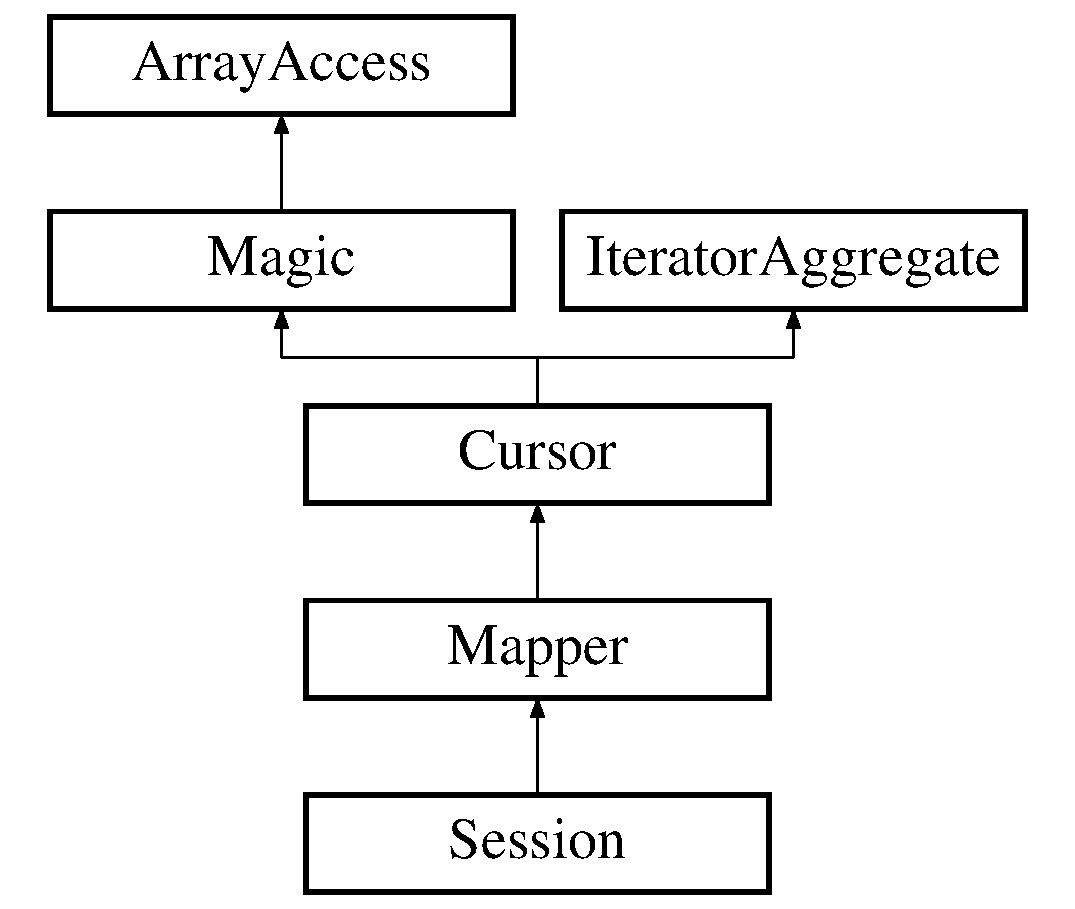
\includegraphics[height=5.000000cm]{class_d_b_1_1_jig_1_1_mapper}
\end{center}
\end{figure}
\subsection*{Public Member Functions}
\begin{DoxyCompactItemize}
\item 
\hyperlink{class_d_b_1_1_jig_1_1_mapper_a38948c2fb1711f49b72f123cbd91e611}{dbtype} ()
\item 
\hyperlink{class_d_b_1_1_jig_1_1_mapper_ace1ae5be37bf26c172cc7ea4e1a65e26}{exists} (\$key)
\item 
\hyperlink{class_d_b_1_1_jig_1_1_mapper_ac8d8012023e560c81f55a629022cb65a}{set} (\$key, \$val)
\item 
\& \hyperlink{class_d_b_1_1_jig_1_1_mapper_ac3695923790b06917410e205068b8376}{get} (\$key)
\item 
\hyperlink{class_d_b_1_1_jig_1_1_mapper_a10a949ef75de6c82c98ac555f371ba83}{clear} (\$key)
\item 
\hyperlink{class_d_b_1_1_jig_1_1_mapper_aa33294a722f17e6e4946223bb73f13ab}{cast} (\$obj=N\+U\+LL)
\item 
\hyperlink{class_d_b_1_1_jig_1_1_mapper_a0a17b08b524058f3c3ce29d0985e83d6}{token} (\$str)
\item 
\hyperlink{class_d_b_1_1_jig_1_1_mapper_ad2b647dea97780ff7a831670ff6ba7dc}{find} (\$filter=N\+U\+LL, array \$options=N\+U\+LL, \$ttl=0, \$\hyperlink{class_d_b_1_1_jig_a92faa80a7077936bd630e5dcc7bb4a64}{log}=T\+R\+UE)
\item 
\hyperlink{class_d_b_1_1_jig_1_1_mapper_ab1f3a3bd85dca49dceaea57f2fe21abf}{count} (\$filter=N\+U\+LL, \$ttl=0)
\item 
\hyperlink{class_d_b_1_1_jig_1_1_mapper_aad399d205074eaeed711d5e0157b3c0a}{skip} (\$ofs=1)
\item 
\hyperlink{class_d_b_1_1_jig_1_1_mapper_a473241246338cfccc4709ba896749019}{insert} ()
\item 
\hyperlink{class_d_b_1_1_jig_1_1_mapper_a842e4774e3b3601a005b995c02f7e883}{update} ()
\item 
\hyperlink{class_d_b_1_1_jig_1_1_mapper_aa7210074cfc1eda78dc492d8b8a96616}{erase} (\$filter=N\+U\+LL)
\item 
\hyperlink{class_d_b_1_1_jig_1_1_mapper_a4a20559544fdf4dcb457e258dc976cf8}{reset} ()
\item 
\hyperlink{class_d_b_1_1_jig_1_1_mapper_adffe904ab38af888d9b033647ec6d935}{copyfrom} (\$var, \$func=N\+U\+LL)
\item 
\hyperlink{class_d_b_1_1_jig_1_1_mapper_a4bcf54f913758fb093c35ea81fc29615}{copyto} (\$key)
\item 
\hyperlink{class_d_b_1_1_jig_1_1_mapper_a9dfc1601eaf8348bed6ba5622f725971}{fields} ()
\item 
\hyperlink{class_d_b_1_1_jig_1_1_mapper_a7f835c25df4cb49d02328644722656da}{getiterator} ()
\item 
\hyperlink{class_d_b_1_1_jig_1_1_mapper_a19fc308235f36411d08e0c019cddc0ad}{\+\_\+\+\_\+construct} (\textbackslash{}\hyperlink{class_d_b_1_1_jig}{D\+B\textbackslash{}\+Jig} \$db, \$file)
\end{DoxyCompactItemize}
\subsection*{Data Fields}
\begin{DoxyCompactItemize}
\item 
\hypertarget{class_d_b_1_1_jig_1_1_mapper_aa1bfbd27060176201b271918dff57e8f}{}\label{class_d_b_1_1_jig_1_1_mapper_aa1bfbd27060176201b271918dff57e8f} 
\hyperlink{class_d_b_1_1_jig_1_1_mapper_aa1bfbd27060176201b271918dff57e8f}{\$file}
\begin{DoxyCompactList}\small\item\em Data file. \end{DoxyCompactList}\item 
\hypertarget{class_d_b_1_1_jig_1_1_mapper_ae97941710d863131c700f069b109991e}{}\label{class_d_b_1_1_jig_1_1_mapper_ae97941710d863131c700f069b109991e} 
\hyperlink{class_d_b_1_1_jig_1_1_mapper_ae97941710d863131c700f069b109991e}{\$id}
\begin{DoxyCompactList}\small\item\em Document identifier. \end{DoxyCompactList}\item 
\hypertarget{class_d_b_1_1_jig_1_1_mapper_ac5a31edb787609a3143dec9bfa8063ea}{}\label{class_d_b_1_1_jig_1_1_mapper_ac5a31edb787609a3143dec9bfa8063ea} 
\hyperlink{class_d_b_1_1_jig_1_1_mapper_ac5a31edb787609a3143dec9bfa8063ea}{\$document} =\mbox{[}$\,$\mbox{]}
\begin{DoxyCompactList}\small\item\em Document contents. \end{DoxyCompactList}\end{DoxyCompactItemize}
\subsection*{Protected Member Functions}
\begin{DoxyCompactItemize}
\item 
\hyperlink{class_d_b_1_1_jig_1_1_mapper_a42470c7265ee40e95bb2beed36d8c7c9}{factory} (\$id, \$row)
\end{DoxyCompactItemize}
\subsection*{Protected Attributes}
\begin{DoxyCompactItemize}
\item 
\hypertarget{class_d_b_1_1_jig_1_1_mapper_a1fa3127fc82f96b1436d871ef02be319}{}\label{class_d_b_1_1_jig_1_1_mapper_a1fa3127fc82f96b1436d871ef02be319} 
\hyperlink{class_d_b_1_1_jig_1_1_mapper_a1fa3127fc82f96b1436d871ef02be319}{\$db}
\begin{DoxyCompactList}\small\item\em Flat-\/file DB wrapper. \end{DoxyCompactList}\end{DoxyCompactItemize}


\subsection{Detailed Description}
Flat-\/file DB mapper. 

Definition at line 26 of file mapper.\+php.



\subsection{Constructor \& Destructor Documentation}
\hypertarget{class_d_b_1_1_jig_1_1_mapper_a19fc308235f36411d08e0c019cddc0ad}{}\label{class_d_b_1_1_jig_1_1_mapper_a19fc308235f36411d08e0c019cddc0ad} 
\index{D\+B\+::\+Jig\+::\+Mapper@{D\+B\+::\+Jig\+::\+Mapper}!\+\_\+\+\_\+construct@{\+\_\+\+\_\+construct}}
\index{\+\_\+\+\_\+construct@{\+\_\+\+\_\+construct}!D\+B\+::\+Jig\+::\+Mapper@{D\+B\+::\+Jig\+::\+Mapper}}
\subsubsection{\texorpdfstring{\+\_\+\+\_\+construct()}{\_\_construct()}}
{\footnotesize\ttfamily \+\_\+\+\_\+construct (\begin{DoxyParamCaption}\item[{\textbackslash{}\hyperlink{class_d_b_1_1_jig}{D\+B\textbackslash{}\+Jig}}]{\$db,  }\item[{}]{\$file }\end{DoxyParamCaption})}

Instantiate class \begin{DoxyReturn}{Returns}
void 
\end{DoxyReturn}

\begin{DoxyParams}{Parameters}
{\em \$db} & object \\
\hline
{\em \$file} & string \\
\hline
\end{DoxyParams}


Definition at line 470 of file mapper.\+php.



\subsection{Member Function Documentation}
\hypertarget{class_d_b_1_1_jig_1_1_mapper_aa33294a722f17e6e4946223bb73f13ab}{}\label{class_d_b_1_1_jig_1_1_mapper_aa33294a722f17e6e4946223bb73f13ab} 
\index{D\+B\+::\+Jig\+::\+Mapper@{D\+B\+::\+Jig\+::\+Mapper}!cast@{cast}}
\index{cast@{cast}!D\+B\+::\+Jig\+::\+Mapper@{D\+B\+::\+Jig\+::\+Mapper}}
\subsubsection{\texorpdfstring{cast()}{cast()}}
{\footnotesize\ttfamily cast (\begin{DoxyParamCaption}\item[{}]{\$obj = {\ttfamily NULL} }\end{DoxyParamCaption})}

Return fields of mapper object as an associative array \begin{DoxyReturn}{Returns}
array 
\end{DoxyReturn}

\begin{DoxyParams}{Parameters}
{\em \$obj} & object \\
\hline
\end{DoxyParams}


Definition at line 111 of file mapper.\+php.

\hypertarget{class_d_b_1_1_jig_1_1_mapper_a10a949ef75de6c82c98ac555f371ba83}{}\label{class_d_b_1_1_jig_1_1_mapper_a10a949ef75de6c82c98ac555f371ba83} 
\index{D\+B\+::\+Jig\+::\+Mapper@{D\+B\+::\+Jig\+::\+Mapper}!clear@{clear}}
\index{clear@{clear}!D\+B\+::\+Jig\+::\+Mapper@{D\+B\+::\+Jig\+::\+Mapper}}
\subsubsection{\texorpdfstring{clear()}{clear()}}
{\footnotesize\ttfamily clear (\begin{DoxyParamCaption}\item[{}]{\$key }\end{DoxyParamCaption})}

Delete field \begin{DoxyReturn}{Returns}
N\+U\+LL 
\end{DoxyReturn}

\begin{DoxyParams}{Parameters}
{\em \$key} & string \\
\hline
\end{DoxyParams}


Definition at line 83 of file mapper.\+php.

\hypertarget{class_d_b_1_1_jig_1_1_mapper_adffe904ab38af888d9b033647ec6d935}{}\label{class_d_b_1_1_jig_1_1_mapper_adffe904ab38af888d9b033647ec6d935} 
\index{D\+B\+::\+Jig\+::\+Mapper@{D\+B\+::\+Jig\+::\+Mapper}!copyfrom@{copyfrom}}
\index{copyfrom@{copyfrom}!D\+B\+::\+Jig\+::\+Mapper@{D\+B\+::\+Jig\+::\+Mapper}}
\subsubsection{\texorpdfstring{copyfrom()}{copyfrom()}}
{\footnotesize\ttfamily copyfrom (\begin{DoxyParamCaption}\item[{}]{\$var,  }\item[{}]{\$func = {\ttfamily NULL} }\end{DoxyParamCaption})}

Hydrate mapper object using hive array variable \begin{DoxyReturn}{Returns}
N\+U\+LL 
\end{DoxyReturn}

\begin{DoxyParams}{Parameters}
{\em \$var} & array$\vert$string \\
\hline
{\em \$func} & callback \\
\hline
\end{DoxyParams}


Definition at line 428 of file mapper.\+php.

\hypertarget{class_d_b_1_1_jig_1_1_mapper_a4bcf54f913758fb093c35ea81fc29615}{}\label{class_d_b_1_1_jig_1_1_mapper_a4bcf54f913758fb093c35ea81fc29615} 
\index{D\+B\+::\+Jig\+::\+Mapper@{D\+B\+::\+Jig\+::\+Mapper}!copyto@{copyto}}
\index{copyto@{copyto}!D\+B\+::\+Jig\+::\+Mapper@{D\+B\+::\+Jig\+::\+Mapper}}
\subsubsection{\texorpdfstring{copyto()}{copyto()}}
{\footnotesize\ttfamily copyto (\begin{DoxyParamCaption}\item[{}]{\$key }\end{DoxyParamCaption})}

Populate hive array variable with mapper fields \begin{DoxyReturn}{Returns}
N\+U\+LL 
\end{DoxyReturn}

\begin{DoxyParams}{Parameters}
{\em \$key} & string \\
\hline
\end{DoxyParams}


Definition at line 442 of file mapper.\+php.

\hypertarget{class_d_b_1_1_jig_1_1_mapper_ab1f3a3bd85dca49dceaea57f2fe21abf}{}\label{class_d_b_1_1_jig_1_1_mapper_ab1f3a3bd85dca49dceaea57f2fe21abf} 
\index{D\+B\+::\+Jig\+::\+Mapper@{D\+B\+::\+Jig\+::\+Mapper}!count@{count}}
\index{count@{count}!D\+B\+::\+Jig\+::\+Mapper@{D\+B\+::\+Jig\+::\+Mapper}}
\subsubsection{\texorpdfstring{count()}{count()}}
{\footnotesize\ttfamily count (\begin{DoxyParamCaption}\item[{}]{\$filter = {\ttfamily NULL},  }\item[{}]{\$ttl = {\ttfamily 0} }\end{DoxyParamCaption})}

Count records that match criteria \begin{DoxyReturn}{Returns}
int 
\end{DoxyReturn}

\begin{DoxyParams}{Parameters}
{\em \$filter} & array \\
\hline
{\em \$ttl} & int \\
\hline
\end{DoxyParams}


Definition at line 291 of file mapper.\+php.

\hypertarget{class_d_b_1_1_jig_1_1_mapper_a38948c2fb1711f49b72f123cbd91e611}{}\label{class_d_b_1_1_jig_1_1_mapper_a38948c2fb1711f49b72f123cbd91e611} 
\index{D\+B\+::\+Jig\+::\+Mapper@{D\+B\+::\+Jig\+::\+Mapper}!dbtype@{dbtype}}
\index{dbtype@{dbtype}!D\+B\+::\+Jig\+::\+Mapper@{D\+B\+::\+Jig\+::\+Mapper}}
\subsubsection{\texorpdfstring{dbtype()}{dbtype()}}
{\footnotesize\ttfamily dbtype (\begin{DoxyParamCaption}{ }\end{DoxyParamCaption})}

Return database type \begin{DoxyReturn}{Returns}
string 
\end{DoxyReturn}


Definition at line 42 of file mapper.\+php.

\hypertarget{class_d_b_1_1_jig_1_1_mapper_aa7210074cfc1eda78dc492d8b8a96616}{}\label{class_d_b_1_1_jig_1_1_mapper_aa7210074cfc1eda78dc492d8b8a96616} 
\index{D\+B\+::\+Jig\+::\+Mapper@{D\+B\+::\+Jig\+::\+Mapper}!erase@{erase}}
\index{erase@{erase}!D\+B\+::\+Jig\+::\+Mapper@{D\+B\+::\+Jig\+::\+Mapper}}
\subsubsection{\texorpdfstring{erase()}{erase()}}
{\footnotesize\ttfamily erase (\begin{DoxyParamCaption}\item[{}]{\$filter = {\ttfamily NULL} }\end{DoxyParamCaption})}

Delete current record \begin{DoxyReturn}{Returns}
bool 
\end{DoxyReturn}

\begin{DoxyParams}{Parameters}
{\em \$filter} & array \\
\hline
\end{DoxyParams}


Definition at line 370 of file mapper.\+php.

\hypertarget{class_d_b_1_1_jig_1_1_mapper_ace1ae5be37bf26c172cc7ea4e1a65e26}{}\label{class_d_b_1_1_jig_1_1_mapper_ace1ae5be37bf26c172cc7ea4e1a65e26} 
\index{D\+B\+::\+Jig\+::\+Mapper@{D\+B\+::\+Jig\+::\+Mapper}!exists@{exists}}
\index{exists@{exists}!D\+B\+::\+Jig\+::\+Mapper@{D\+B\+::\+Jig\+::\+Mapper}}
\subsubsection{\texorpdfstring{exists()}{exists()}}
{\footnotesize\ttfamily exists (\begin{DoxyParamCaption}\item[{}]{\$key }\end{DoxyParamCaption})}

Return T\+R\+UE if field is defined \begin{DoxyReturn}{Returns}
bool 
\end{DoxyReturn}

\begin{DoxyParams}{Parameters}
{\em \$key} & string \\
\hline
\end{DoxyParams}


Definition at line 51 of file mapper.\+php.

\hypertarget{class_d_b_1_1_jig_1_1_mapper_a42470c7265ee40e95bb2beed36d8c7c9}{}\label{class_d_b_1_1_jig_1_1_mapper_a42470c7265ee40e95bb2beed36d8c7c9} 
\index{D\+B\+::\+Jig\+::\+Mapper@{D\+B\+::\+Jig\+::\+Mapper}!factory@{factory}}
\index{factory@{factory}!D\+B\+::\+Jig\+::\+Mapper@{D\+B\+::\+Jig\+::\+Mapper}}
\subsubsection{\texorpdfstring{factory()}{factory()}}
{\footnotesize\ttfamily factory (\begin{DoxyParamCaption}\item[{}]{\$id,  }\item[{}]{\$row }\end{DoxyParamCaption})\hspace{0.3cm}{\ttfamily [protected]}}

Convert array to mapper object \begin{DoxyReturn}{Returns}
object 
\end{DoxyReturn}

\begin{DoxyParams}{Parameters}
{\em \$id} & string \\
\hline
{\em \$row} & array \\
\hline
\end{DoxyParams}


Definition at line 94 of file mapper.\+php.

\hypertarget{class_d_b_1_1_jig_1_1_mapper_a9dfc1601eaf8348bed6ba5622f725971}{}\label{class_d_b_1_1_jig_1_1_mapper_a9dfc1601eaf8348bed6ba5622f725971} 
\index{D\+B\+::\+Jig\+::\+Mapper@{D\+B\+::\+Jig\+::\+Mapper}!fields@{fields}}
\index{fields@{fields}!D\+B\+::\+Jig\+::\+Mapper@{D\+B\+::\+Jig\+::\+Mapper}}
\subsubsection{\texorpdfstring{fields()}{fields()}}
{\footnotesize\ttfamily fields (\begin{DoxyParamCaption}{ }\end{DoxyParamCaption})}

Return field names \begin{DoxyReturn}{Returns}
array 
\end{DoxyReturn}


Definition at line 452 of file mapper.\+php.

\hypertarget{class_d_b_1_1_jig_1_1_mapper_ad2b647dea97780ff7a831670ff6ba7dc}{}\label{class_d_b_1_1_jig_1_1_mapper_ad2b647dea97780ff7a831670ff6ba7dc} 
\index{D\+B\+::\+Jig\+::\+Mapper@{D\+B\+::\+Jig\+::\+Mapper}!find@{find}}
\index{find@{find}!D\+B\+::\+Jig\+::\+Mapper@{D\+B\+::\+Jig\+::\+Mapper}}
\subsubsection{\texorpdfstring{find()}{find()}}
{\footnotesize\ttfamily find (\begin{DoxyParamCaption}\item[{}]{\$filter = {\ttfamily NULL},  }\item[{array}]{\$options = {\ttfamily NULL},  }\item[{}]{\$ttl = {\ttfamily 0},  }\item[{}]{\$log = {\ttfamily TRUE} }\end{DoxyParamCaption})}

Return records that match criteria \begin{DoxyReturn}{Returns}
static\mbox{[}\mbox{]}$\vert$\+F\+A\+L\+SE 
\end{DoxyReturn}

\begin{DoxyParams}{Parameters}
{\em \$filter} & array \\
\hline
{\em \$options} & array \\
\hline
{\em \$ttl} & int \\
\hline
{\em \$log} & bool \\
\hline
\end{DoxyParams}


Definition at line 158 of file mapper.\+php.

\hypertarget{class_d_b_1_1_jig_1_1_mapper_ac3695923790b06917410e205068b8376}{}\label{class_d_b_1_1_jig_1_1_mapper_ac3695923790b06917410e205068b8376} 
\index{D\+B\+::\+Jig\+::\+Mapper@{D\+B\+::\+Jig\+::\+Mapper}!get@{get}}
\index{get@{get}!D\+B\+::\+Jig\+::\+Mapper@{D\+B\+::\+Jig\+::\+Mapper}}
\subsubsection{\texorpdfstring{get()}{get()}}
{\footnotesize\ttfamily \& get (\begin{DoxyParamCaption}\item[{}]{\$key }\end{DoxyParamCaption})}

Retrieve value of field \begin{DoxyReturn}{Returns}
scalar$\vert$\+F\+A\+L\+SE 
\end{DoxyReturn}

\begin{DoxyParams}{Parameters}
{\em \$key} & string \\
\hline
\end{DoxyParams}


Definition at line 70 of file mapper.\+php.

\hypertarget{class_d_b_1_1_jig_1_1_mapper_a7f835c25df4cb49d02328644722656da}{}\label{class_d_b_1_1_jig_1_1_mapper_a7f835c25df4cb49d02328644722656da} 
\index{D\+B\+::\+Jig\+::\+Mapper@{D\+B\+::\+Jig\+::\+Mapper}!getiterator@{getiterator}}
\index{getiterator@{getiterator}!D\+B\+::\+Jig\+::\+Mapper@{D\+B\+::\+Jig\+::\+Mapper}}
\subsubsection{\texorpdfstring{getiterator()}{getiterator()}}
{\footnotesize\ttfamily getiterator (\begin{DoxyParamCaption}{ }\end{DoxyParamCaption})}

Retrieve external iterator for fields \begin{DoxyReturn}{Returns}
object 
\end{DoxyReturn}


Definition at line 460 of file mapper.\+php.

\hypertarget{class_d_b_1_1_jig_1_1_mapper_a473241246338cfccc4709ba896749019}{}\label{class_d_b_1_1_jig_1_1_mapper_a473241246338cfccc4709ba896749019} 
\index{D\+B\+::\+Jig\+::\+Mapper@{D\+B\+::\+Jig\+::\+Mapper}!insert@{insert}}
\index{insert@{insert}!D\+B\+::\+Jig\+::\+Mapper@{D\+B\+::\+Jig\+::\+Mapper}}
\subsubsection{\texorpdfstring{insert()}{insert()}}
{\footnotesize\ttfamily insert (\begin{DoxyParamCaption}{ }\end{DoxyParamCaption})}

Insert new record \begin{DoxyReturn}{Returns}
array 
\end{DoxyReturn}


Definition at line 317 of file mapper.\+php.

\hypertarget{class_d_b_1_1_jig_1_1_mapper_a4a20559544fdf4dcb457e258dc976cf8}{}\label{class_d_b_1_1_jig_1_1_mapper_a4a20559544fdf4dcb457e258dc976cf8} 
\index{D\+B\+::\+Jig\+::\+Mapper@{D\+B\+::\+Jig\+::\+Mapper}!reset@{reset}}
\index{reset@{reset}!D\+B\+::\+Jig\+::\+Mapper@{D\+B\+::\+Jig\+::\+Mapper}}
\subsubsection{\texorpdfstring{reset()}{reset()}}
{\footnotesize\ttfamily reset (\begin{DoxyParamCaption}{ }\end{DoxyParamCaption})}

Reset cursor \begin{DoxyReturn}{Returns}
N\+U\+LL 
\end{DoxyReturn}


Definition at line 416 of file mapper.\+php.

\hypertarget{class_d_b_1_1_jig_1_1_mapper_ac8d8012023e560c81f55a629022cb65a}{}\label{class_d_b_1_1_jig_1_1_mapper_ac8d8012023e560c81f55a629022cb65a} 
\index{D\+B\+::\+Jig\+::\+Mapper@{D\+B\+::\+Jig\+::\+Mapper}!set@{set}}
\index{set@{set}!D\+B\+::\+Jig\+::\+Mapper@{D\+B\+::\+Jig\+::\+Mapper}}
\subsubsection{\texorpdfstring{set()}{set()}}
{\footnotesize\ttfamily set (\begin{DoxyParamCaption}\item[{}]{\$key,  }\item[{}]{\$val }\end{DoxyParamCaption})}

Assign value to field \begin{DoxyReturn}{Returns}
scalar$\vert$\+F\+A\+L\+SE 
\end{DoxyReturn}

\begin{DoxyParams}{Parameters}
{\em \$key} & string \\
\hline
{\em \$val} & scalar \\
\hline
\end{DoxyParams}


Definition at line 61 of file mapper.\+php.

\hypertarget{class_d_b_1_1_jig_1_1_mapper_aad399d205074eaeed711d5e0157b3c0a}{}\label{class_d_b_1_1_jig_1_1_mapper_aad399d205074eaeed711d5e0157b3c0a} 
\index{D\+B\+::\+Jig\+::\+Mapper@{D\+B\+::\+Jig\+::\+Mapper}!skip@{skip}}
\index{skip@{skip}!D\+B\+::\+Jig\+::\+Mapper@{D\+B\+::\+Jig\+::\+Mapper}}
\subsubsection{\texorpdfstring{skip()}{skip()}}
{\footnotesize\ttfamily skip (\begin{DoxyParamCaption}\item[{}]{\$ofs = {\ttfamily 1} }\end{DoxyParamCaption})}

Return record at specified offset using criteria of previous \hyperlink{class_d_b_1_1_cursor_a4db66c122e6274a3d653eff639e8476f}{load()} call and make it active \begin{DoxyReturn}{Returns}
array 
\end{DoxyReturn}

\begin{DoxyParams}{Parameters}
{\em \$ofs} & int \\
\hline
\end{DoxyParams}


Definition at line 305 of file mapper.\+php.

\hypertarget{class_d_b_1_1_jig_1_1_mapper_a0a17b08b524058f3c3ce29d0985e83d6}{}\label{class_d_b_1_1_jig_1_1_mapper_a0a17b08b524058f3c3ce29d0985e83d6} 
\index{D\+B\+::\+Jig\+::\+Mapper@{D\+B\+::\+Jig\+::\+Mapper}!token@{token}}
\index{token@{token}!D\+B\+::\+Jig\+::\+Mapper@{D\+B\+::\+Jig\+::\+Mapper}}
\subsubsection{\texorpdfstring{token()}{token()}}
{\footnotesize\ttfamily token (\begin{DoxyParamCaption}\item[{}]{\$str }\end{DoxyParamCaption})}

Convert tokens in string expression to variable names \begin{DoxyReturn}{Returns}
string 
\end{DoxyReturn}

\begin{DoxyParams}{Parameters}
{\em \$str} & string \\
\hline
\end{DoxyParams}


Definition at line 122 of file mapper.\+php.

\hypertarget{class_d_b_1_1_jig_1_1_mapper_a842e4774e3b3601a005b995c02f7e883}{}\label{class_d_b_1_1_jig_1_1_mapper_a842e4774e3b3601a005b995c02f7e883} 
\index{D\+B\+::\+Jig\+::\+Mapper@{D\+B\+::\+Jig\+::\+Mapper}!update@{update}}
\index{update@{update}!D\+B\+::\+Jig\+::\+Mapper@{D\+B\+::\+Jig\+::\+Mapper}}
\subsubsection{\texorpdfstring{update()}{update()}}
{\footnotesize\ttfamily update (\begin{DoxyParamCaption}{ }\end{DoxyParamCaption})}

Update current record \begin{DoxyReturn}{Returns}
array 
\end{DoxyReturn}


Definition at line 347 of file mapper.\+php.



The documentation for this class was generated from the following file\+:\begin{DoxyCompactItemize}
\item 
/\+Users/aplennevaux/\+G\+I\+T\+H\+U\+B/\+Visionary-\/website/src/vendor/bcosca/fatfree/lib/db/jig/mapper.\+php\end{DoxyCompactItemize}

\hypertarget{class_markdown}{}\section{Markdown Class Reference}
\label{class_markdown}\index{Markdown@{Markdown}}


Markdown-\/to-\/\+H\+T\+ML converter.  


Inheritance diagram for Markdown\+:\begin{figure}[H]
\begin{center}
\leavevmode
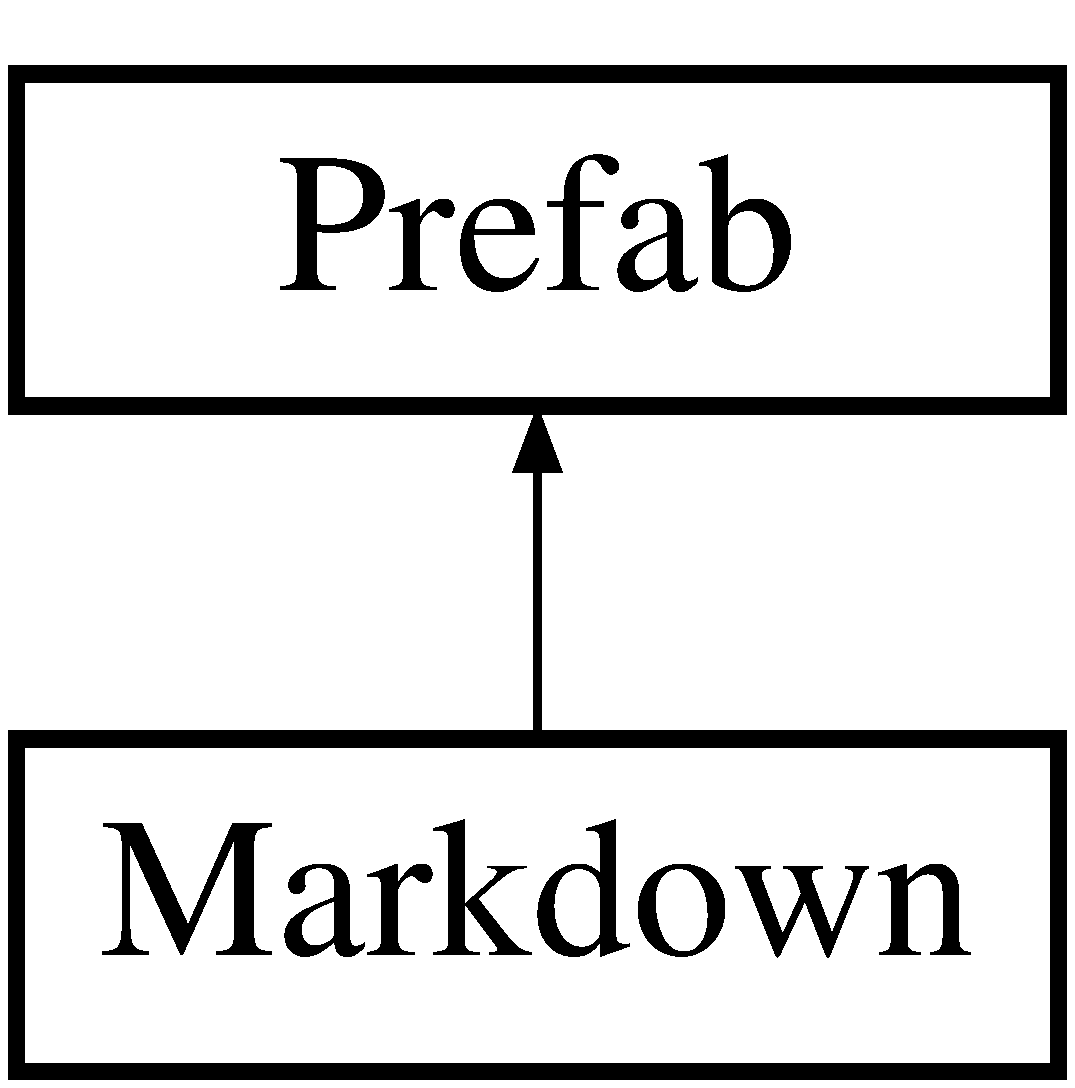
\includegraphics[height=2.000000cm]{class_markdown}
\end{center}
\end{figure}
\subsection*{Public Member Functions}
\begin{DoxyCompactItemize}
\item 
\hyperlink{class_markdown_a5c55a8c8fce867d0889971aaaf590040}{esc} (\$str)
\item 
\hyperlink{class_markdown_a13c88b9c8e8002dfc54d002e47baf4fc}{scan} (\$str)
\item 
\hyperlink{class_markdown_a64ffc5ca8440ddf7e0f3b3f03c16edf2}{convert} (\$txt)
\end{DoxyCompactItemize}
\subsection*{Data Fields}
\begin{DoxyCompactItemize}
\item 
\hypertarget{class_markdown_aac9b8e6c2865946aa0c0155dfbd03c99}{}\label{class_markdown_aac9b8e6c2865946aa0c0155dfbd03c99} 
\hyperlink{class_markdown_aac9b8e6c2865946aa0c0155dfbd03c99}{\$special}
\begin{DoxyCompactList}\small\item\em Special characters. \end{DoxyCompactList}\end{DoxyCompactItemize}
\subsection*{Protected Member Functions}
\begin{DoxyCompactItemize}
\item 
\hyperlink{class_markdown_a9130181ea7718ddb9a253c1c58709e62}{\+\_\+blockquote} (\$str)
\item 
\hyperlink{class_markdown_a2f41e07d6b78f3e9b882bcb34792446d}{\+\_\+pre} (\$str)
\item 
\hyperlink{class_markdown_a18b5eb148af09b928ec07484646f3131}{\+\_\+fence} (\$hint, \$str)
\item 
\hyperlink{class_markdown_a794a9d5fa6b867db9eaecd18fa8394de}{\+\_\+hr} ()
\item 
\hyperlink{class_markdown_a1018c6d4736c90992988a353d3f0edf3}{\+\_\+atx} (\$type, \$str)
\item 
\hyperlink{class_markdown_ad20b6a50b2c1d6b92556755efae0d5ae}{\+\_\+setext} (\$str, \$type)
\item 
\hyperlink{class_markdown_acd211dbc64fbdc856e4abd46670f6993}{\+\_\+li} (\$str)
\item 
\hyperlink{class_markdown_aa1fa1fb7287331de41bc0c75fa349afa}{\+\_\+raw} (\$str)
\item 
\hyperlink{class_markdown_a82a2bccde5a674e56ab6c6c3be76273c}{\+\_\+p} (\$str)
\item 
\hyperlink{class_markdown_a11f2b2c375b61a22398e08bdb95aa4b6}{\+\_\+text} (\$str)
\item 
\hyperlink{class_markdown_a29692127c6b62aed5fba05bc7d2aba5f}{\+\_\+img} (\$str)
\item 
\hyperlink{class_markdown_a65692f4b6b15029d6e26a80db9e4748c}{\+\_\+a} (\$str)
\item 
\hyperlink{class_markdown_ad228c71c9aae197fda9b32413b63e605}{\+\_\+auto} (\$str)
\item 
\hyperlink{class_markdown_a8cd84bea585e81d80e4dfb8836922e54}{\+\_\+code} (\$str)
\item 
\hyperlink{class_markdown_aa662980c0756e03123234999df984f02}{snip} (\$str)
\item 
\hyperlink{class_markdown_aeafac9b9cffe924ba0f859a6bfb8aa85}{build} (\$str)
\end{DoxyCompactItemize}
\subsection*{Protected Attributes}
\begin{DoxyCompactItemize}
\item 
\hypertarget{class_markdown_a320aeae1df42ee73ab4b3d9f7cf4ef3f}{}\label{class_markdown_a320aeae1df42ee73ab4b3d9f7cf4ef3f} 
\hyperlink{class_markdown_a320aeae1df42ee73ab4b3d9f7cf4ef3f}{\$blocks}
\begin{DoxyCompactList}\small\item\em Parsing rules. \end{DoxyCompactList}\end{DoxyCompactItemize}
\subsection*{Additional Inherited Members}


\subsection{Detailed Description}
Markdown-\/to-\/\+H\+T\+ML converter. 

Definition at line 24 of file markdown.\+php.



\subsection{Member Function Documentation}
\hypertarget{class_markdown_a65692f4b6b15029d6e26a80db9e4748c}{}\label{class_markdown_a65692f4b6b15029d6e26a80db9e4748c} 
\index{Markdown@{Markdown}!\+\_\+a@{\+\_\+a}}
\index{\+\_\+a@{\+\_\+a}!Markdown@{Markdown}}
\subsubsection{\texorpdfstring{\+\_\+a()}{\_a()}}
{\footnotesize\ttfamily \+\_\+a (\begin{DoxyParamCaption}\item[{}]{\$str }\end{DoxyParamCaption})\hspace{0.3cm}{\ttfamily [protected]}}

Process anchor span \begin{DoxyReturn}{Returns}
string 
\end{DoxyReturn}

\begin{DoxyParams}{Parameters}
{\em \$str} & string \\
\hline
\end{DoxyParams}


Definition at line 371 of file markdown.\+php.

\hypertarget{class_markdown_a1018c6d4736c90992988a353d3f0edf3}{}\label{class_markdown_a1018c6d4736c90992988a353d3f0edf3} 
\index{Markdown@{Markdown}!\+\_\+atx@{\+\_\+atx}}
\index{\+\_\+atx@{\+\_\+atx}!Markdown@{Markdown}}
\subsubsection{\texorpdfstring{\+\_\+atx()}{\_atx()}}
{\footnotesize\ttfamily \+\_\+atx (\begin{DoxyParamCaption}\item[{}]{\$type,  }\item[{}]{\$str }\end{DoxyParamCaption})\hspace{0.3cm}{\ttfamily [protected]}}

Process atx-\/style heading \begin{DoxyReturn}{Returns}
string 
\end{DoxyReturn}

\begin{DoxyParams}{Parameters}
{\em \$type} & string \\
\hline
{\em \$str} & string \\
\hline
\end{DoxyParams}


Definition at line 194 of file markdown.\+php.

\hypertarget{class_markdown_ad228c71c9aae197fda9b32413b63e605}{}\label{class_markdown_ad228c71c9aae197fda9b32413b63e605} 
\index{Markdown@{Markdown}!\+\_\+auto@{\+\_\+auto}}
\index{\+\_\+auto@{\+\_\+auto}!Markdown@{Markdown}}
\subsubsection{\texorpdfstring{\+\_\+auto()}{\_auto()}}
{\footnotesize\ttfamily \+\_\+auto (\begin{DoxyParamCaption}\item[{}]{\$str }\end{DoxyParamCaption})\hspace{0.3cm}{\ttfamily [protected]}}

Auto-\/convert links \begin{DoxyReturn}{Returns}
string 
\end{DoxyReturn}

\begin{DoxyParams}{Parameters}
{\em \$str} & string \\
\hline
\end{DoxyParams}


Definition at line 391 of file markdown.\+php.

\hypertarget{class_markdown_a9130181ea7718ddb9a253c1c58709e62}{}\label{class_markdown_a9130181ea7718ddb9a253c1c58709e62} 
\index{Markdown@{Markdown}!\+\_\+blockquote@{\+\_\+blockquote}}
\index{\+\_\+blockquote@{\+\_\+blockquote}!Markdown@{Markdown}}
\subsubsection{\texorpdfstring{\+\_\+blockquote()}{\_blockquote()}}
{\footnotesize\ttfamily \+\_\+blockquote (\begin{DoxyParamCaption}\item[{}]{\$str }\end{DoxyParamCaption})\hspace{0.3cm}{\ttfamily [protected]}}

Process blockquote \begin{DoxyReturn}{Returns}
string 
\end{DoxyReturn}

\begin{DoxyParams}{Parameters}
{\em \$str} & string \\
\hline
\end{DoxyParams}


Definition at line 37 of file markdown.\+php.

\hypertarget{class_markdown_a8cd84bea585e81d80e4dfb8836922e54}{}\label{class_markdown_a8cd84bea585e81d80e4dfb8836922e54} 
\index{Markdown@{Markdown}!\+\_\+code@{\+\_\+code}}
\index{\+\_\+code@{\+\_\+code}!Markdown@{Markdown}}
\subsubsection{\texorpdfstring{\+\_\+code()}{\_code()}}
{\footnotesize\ttfamily \+\_\+code (\begin{DoxyParamCaption}\item[{}]{\$str }\end{DoxyParamCaption})\hspace{0.3cm}{\ttfamily [protected]}}

Process code span \begin{DoxyReturn}{Returns}
string 
\end{DoxyReturn}

\begin{DoxyParams}{Parameters}
{\em \$str} & string \\
\hline
\end{DoxyParams}


Definition at line 411 of file markdown.\+php.

\hypertarget{class_markdown_a18b5eb148af09b928ec07484646f3131}{}\label{class_markdown_a18b5eb148af09b928ec07484646f3131} 
\index{Markdown@{Markdown}!\+\_\+fence@{\+\_\+fence}}
\index{\+\_\+fence@{\+\_\+fence}!Markdown@{Markdown}}
\subsubsection{\texorpdfstring{\+\_\+fence()}{\_fence()}}
{\footnotesize\ttfamily \+\_\+fence (\begin{DoxyParamCaption}\item[{}]{\$hint,  }\item[{}]{\$str }\end{DoxyParamCaption})\hspace{0.3cm}{\ttfamily [protected]}}

Process fenced code block \begin{DoxyReturn}{Returns}
string 
\end{DoxyReturn}

\begin{DoxyParams}{Parameters}
{\em \$hint} & string \\
\hline
{\em \$str} & string \\
\hline
\end{DoxyParams}


Definition at line 64 of file markdown.\+php.

\hypertarget{class_markdown_a794a9d5fa6b867db9eaecd18fa8394de}{}\label{class_markdown_a794a9d5fa6b867db9eaecd18fa8394de} 
\index{Markdown@{Markdown}!\+\_\+hr@{\+\_\+hr}}
\index{\+\_\+hr@{\+\_\+hr}!Markdown@{Markdown}}
\subsubsection{\texorpdfstring{\+\_\+hr()}{\_hr()}}
{\footnotesize\ttfamily \+\_\+hr (\begin{DoxyParamCaption}{ }\end{DoxyParamCaption})\hspace{0.3cm}{\ttfamily [protected]}}

Process horizontal rule \begin{DoxyReturn}{Returns}
string 
\end{DoxyReturn}


Definition at line 184 of file markdown.\+php.

\hypertarget{class_markdown_a29692127c6b62aed5fba05bc7d2aba5f}{}\label{class_markdown_a29692127c6b62aed5fba05bc7d2aba5f} 
\index{Markdown@{Markdown}!\+\_\+img@{\+\_\+img}}
\index{\+\_\+img@{\+\_\+img}!Markdown@{Markdown}}
\subsubsection{\texorpdfstring{\+\_\+img()}{\_img()}}
{\footnotesize\ttfamily \+\_\+img (\begin{DoxyParamCaption}\item[{}]{\$str }\end{DoxyParamCaption})\hspace{0.3cm}{\ttfamily [protected]}}

Process image span \begin{DoxyReturn}{Returns}
string 
\end{DoxyReturn}

\begin{DoxyParams}{Parameters}
{\em \$str} & string \\
\hline
\end{DoxyParams}


Definition at line 349 of file markdown.\+php.

\hypertarget{class_markdown_acd211dbc64fbdc856e4abd46670f6993}{}\label{class_markdown_acd211dbc64fbdc856e4abd46670f6993} 
\index{Markdown@{Markdown}!\+\_\+li@{\+\_\+li}}
\index{\+\_\+li@{\+\_\+li}!Markdown@{Markdown}}
\subsubsection{\texorpdfstring{\+\_\+li()}{\_li()}}
{\footnotesize\ttfamily \+\_\+li (\begin{DoxyParamCaption}\item[{}]{\$str }\end{DoxyParamCaption})\hspace{0.3cm}{\ttfamily [protected]}}

Process ordered/unordered list \begin{DoxyReturn}{Returns}
string 
\end{DoxyReturn}

\begin{DoxyParams}{Parameters}
{\em \$str} & string \\
\hline
\end{DoxyParams}


Definition at line 217 of file markdown.\+php.

\hypertarget{class_markdown_a82a2bccde5a674e56ab6c6c3be76273c}{}\label{class_markdown_a82a2bccde5a674e56ab6c6c3be76273c} 
\index{Markdown@{Markdown}!\+\_\+p@{\+\_\+p}}
\index{\+\_\+p@{\+\_\+p}!Markdown@{Markdown}}
\subsubsection{\texorpdfstring{\+\_\+p()}{\_p()}}
{\footnotesize\ttfamily \+\_\+p (\begin{DoxyParamCaption}\item[{}]{\$str }\end{DoxyParamCaption})\hspace{0.3cm}{\ttfamily [protected]}}

Process paragraph \begin{DoxyReturn}{Returns}
string 
\end{DoxyReturn}

\begin{DoxyParams}{Parameters}
{\em \$str} & string \\
\hline
\end{DoxyParams}


Definition at line 286 of file markdown.\+php.

\hypertarget{class_markdown_a2f41e07d6b78f3e9b882bcb34792446d}{}\label{class_markdown_a2f41e07d6b78f3e9b882bcb34792446d} 
\index{Markdown@{Markdown}!\+\_\+pre@{\+\_\+pre}}
\index{\+\_\+pre@{\+\_\+pre}!Markdown@{Markdown}}
\subsubsection{\texorpdfstring{\+\_\+pre()}{\_pre()}}
{\footnotesize\ttfamily \+\_\+pre (\begin{DoxyParamCaption}\item[{}]{\$str }\end{DoxyParamCaption})\hspace{0.3cm}{\ttfamily [protected]}}

Process whitespace-\/prefixed code block \begin{DoxyReturn}{Returns}
string 
\end{DoxyReturn}

\begin{DoxyParams}{Parameters}
{\em \$str} & string \\
\hline
\end{DoxyParams}


Definition at line 48 of file markdown.\+php.

\hypertarget{class_markdown_aa1fa1fb7287331de41bc0c75fa349afa}{}\label{class_markdown_aa1fa1fb7287331de41bc0c75fa349afa} 
\index{Markdown@{Markdown}!\+\_\+raw@{\+\_\+raw}}
\index{\+\_\+raw@{\+\_\+raw}!Markdown@{Markdown}}
\subsubsection{\texorpdfstring{\+\_\+raw()}{\_raw()}}
{\footnotesize\ttfamily \+\_\+raw (\begin{DoxyParamCaption}\item[{}]{\$str }\end{DoxyParamCaption})\hspace{0.3cm}{\ttfamily [protected]}}

Ignore raw H\+T\+ML \begin{DoxyReturn}{Returns}
string 
\end{DoxyReturn}

\begin{DoxyParams}{Parameters}
{\em \$str} & string \\
\hline
\end{DoxyParams}


Definition at line 277 of file markdown.\+php.

\hypertarget{class_markdown_ad20b6a50b2c1d6b92556755efae0d5ae}{}\label{class_markdown_ad20b6a50b2c1d6b92556755efae0d5ae} 
\index{Markdown@{Markdown}!\+\_\+setext@{\+\_\+setext}}
\index{\+\_\+setext@{\+\_\+setext}!Markdown@{Markdown}}
\subsubsection{\texorpdfstring{\+\_\+setext()}{\_setext()}}
{\footnotesize\ttfamily \+\_\+setext (\begin{DoxyParamCaption}\item[{}]{\$str,  }\item[{}]{\$type }\end{DoxyParamCaption})\hspace{0.3cm}{\ttfamily [protected]}}

Process setext-\/style heading \begin{DoxyReturn}{Returns}
string 
\end{DoxyReturn}

\begin{DoxyParams}{Parameters}
{\em \$str} & string \\
\hline
{\em \$type} & string \\
\hline
\end{DoxyParams}


Definition at line 206 of file markdown.\+php.

\hypertarget{class_markdown_a11f2b2c375b61a22398e08bdb95aa4b6}{}\label{class_markdown_a11f2b2c375b61a22398e08bdb95aa4b6} 
\index{Markdown@{Markdown}!\+\_\+text@{\+\_\+text}}
\index{\+\_\+text@{\+\_\+text}!Markdown@{Markdown}}
\subsubsection{\texorpdfstring{\+\_\+text()}{\_text()}}
{\footnotesize\ttfamily \+\_\+text (\begin{DoxyParamCaption}\item[{}]{\$str }\end{DoxyParamCaption})\hspace{0.3cm}{\ttfamily [protected]}}

Process strong/em/strikethrough spans \begin{DoxyReturn}{Returns}
string 
\end{DoxyReturn}

\begin{DoxyParams}{Parameters}
{\em \$str} & string \\
\hline
\end{DoxyParams}


Definition at line 320 of file markdown.\+php.

\hypertarget{class_markdown_aeafac9b9cffe924ba0f859a6bfb8aa85}{}\label{class_markdown_aeafac9b9cffe924ba0f859a6bfb8aa85} 
\index{Markdown@{Markdown}!build@{build}}
\index{build@{build}!Markdown@{Markdown}}
\subsubsection{\texorpdfstring{build()}{build()}}
{\footnotesize\ttfamily build (\begin{DoxyParamCaption}\item[{}]{\$str }\end{DoxyParamCaption})\hspace{0.3cm}{\ttfamily [protected]}}

Assemble blocks \begin{DoxyReturn}{Returns}
string 
\end{DoxyReturn}

\begin{DoxyParams}{Parameters}
{\em \$str} & string \\
\hline
\end{DoxyParams}


Definition at line 468 of file markdown.\+php.

\hypertarget{class_markdown_a64ffc5ca8440ddf7e0f3b3f03c16edf2}{}\label{class_markdown_a64ffc5ca8440ddf7e0f3b3f03c16edf2} 
\index{Markdown@{Markdown}!convert@{convert}}
\index{convert@{convert}!Markdown@{Markdown}}
\subsubsection{\texorpdfstring{convert()}{convert()}}
{\footnotesize\ttfamily convert (\begin{DoxyParamCaption}\item[{}]{\$txt }\end{DoxyParamCaption})}

Render H\+T\+ML equivalent of markdown \begin{DoxyReturn}{Returns}
string 
\end{DoxyReturn}

\begin{DoxyParams}{Parameters}
{\em \$txt} & string \\
\hline
\end{DoxyParams}


Definition at line 563 of file markdown.\+php.

\hypertarget{class_markdown_a5c55a8c8fce867d0889971aaaf590040}{}\label{class_markdown_a5c55a8c8fce867d0889971aaaf590040} 
\index{Markdown@{Markdown}!esc@{esc}}
\index{esc@{esc}!Markdown@{Markdown}}
\subsubsection{\texorpdfstring{esc()}{esc()}}
{\footnotesize\ttfamily esc (\begin{DoxyParamCaption}\item[{}]{\$str }\end{DoxyParamCaption})}

Convert characters to H\+T\+ML entities \begin{DoxyReturn}{Returns}
string 
\end{DoxyReturn}

\begin{DoxyParams}{Parameters}
{\em \$str} & string \\
\hline
\end{DoxyParams}


Definition at line 428 of file markdown.\+php.

\hypertarget{class_markdown_a13c88b9c8e8002dfc54d002e47baf4fc}{}\label{class_markdown_a13c88b9c8e8002dfc54d002e47baf4fc} 
\index{Markdown@{Markdown}!scan@{scan}}
\index{scan@{scan}!Markdown@{Markdown}}
\subsubsection{\texorpdfstring{scan()}{scan()}}
{\footnotesize\ttfamily scan (\begin{DoxyParamCaption}\item[{}]{\$str }\end{DoxyParamCaption})}

Scan line for convertible spans \begin{DoxyReturn}{Returns}
string 
\end{DoxyReturn}

\begin{DoxyParams}{Parameters}
{\em \$str} & string \\
\hline
\end{DoxyParams}


Definition at line 456 of file markdown.\+php.

\hypertarget{class_markdown_aa662980c0756e03123234999df984f02}{}\label{class_markdown_aa662980c0756e03123234999df984f02} 
\index{Markdown@{Markdown}!snip@{snip}}
\index{snip@{snip}!Markdown@{Markdown}}
\subsubsection{\texorpdfstring{snip()}{snip()}}
{\footnotesize\ttfamily snip (\begin{DoxyParamCaption}\item[{}]{\$str }\end{DoxyParamCaption})\hspace{0.3cm}{\ttfamily [protected]}}

Reduce multiple line feeds \begin{DoxyReturn}{Returns}
string 
\end{DoxyReturn}

\begin{DoxyParams}{Parameters}
{\em \$str} & string \\
\hline
\end{DoxyParams}


Definition at line 447 of file markdown.\+php.



The documentation for this class was generated from the following file\+:\begin{DoxyCompactItemize}
\item 
/\+Users/aplennevaux/\+G\+I\+T\+H\+U\+B/\+Visionary-\/website/src/vendor/bcosca/fatfree/lib/markdown.\+php\end{DoxyCompactItemize}

\hypertarget{class_matrix}{}\section{Matrix Class Reference}
\label{class_matrix}\index{Matrix@{Matrix}}


Generic array utilities.  


Inheritance diagram for Matrix\+:\begin{figure}[H]
\begin{center}
\leavevmode
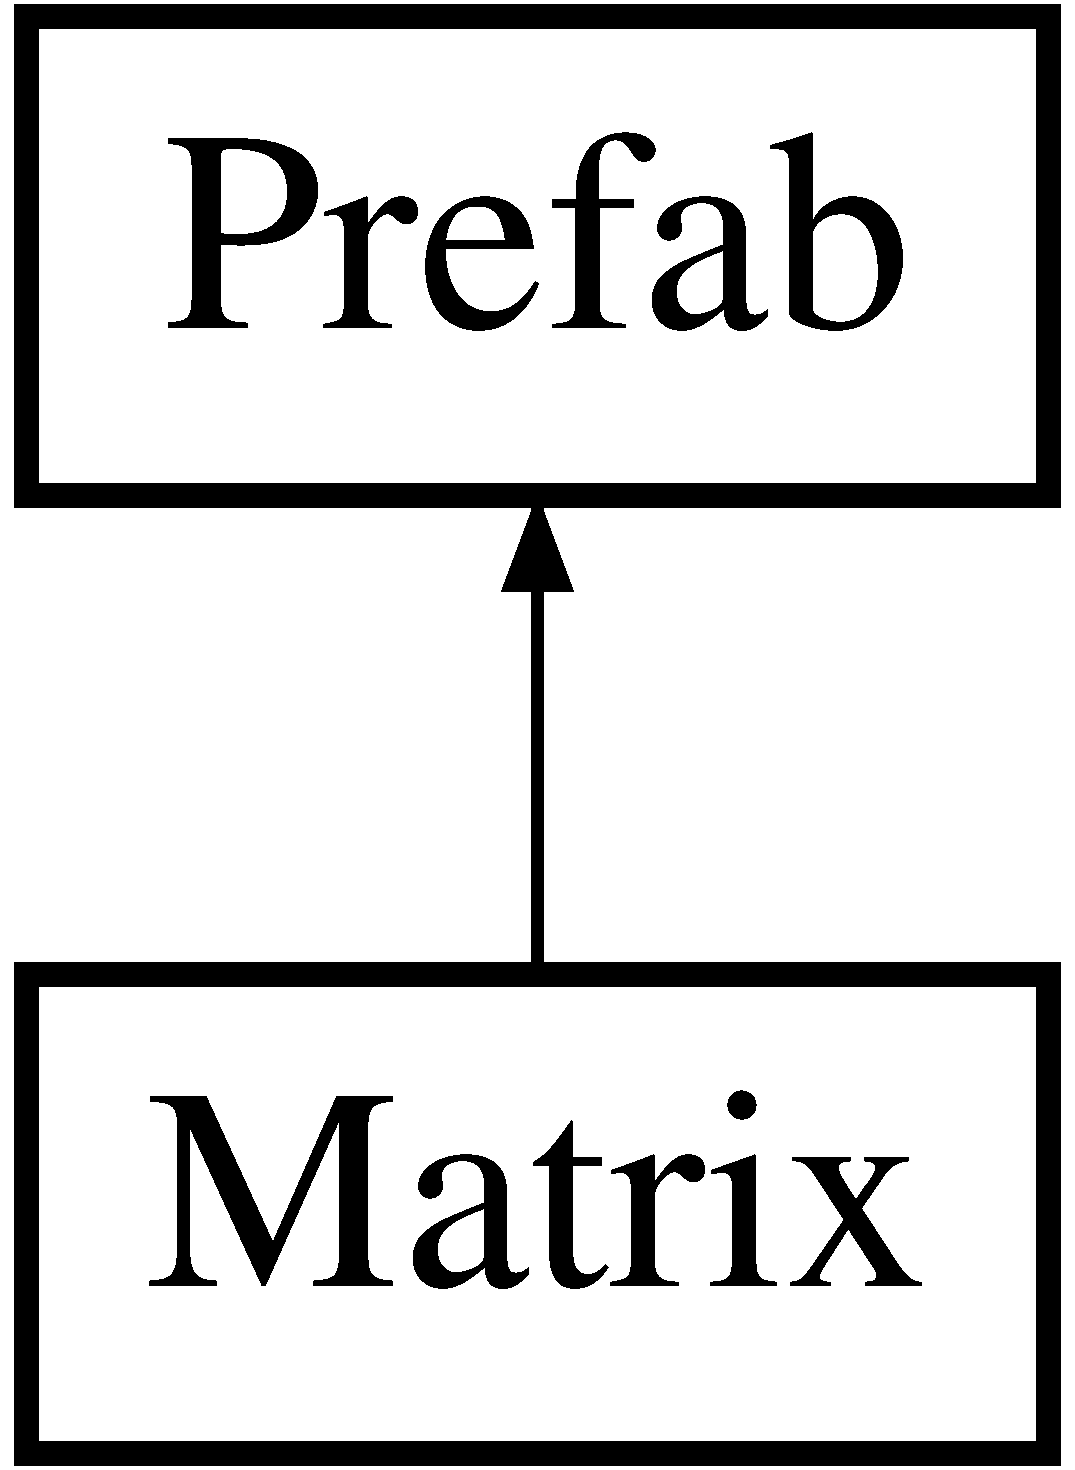
\includegraphics[height=2.000000cm]{class_matrix}
\end{center}
\end{figure}
\subsection*{Public Member Functions}
\begin{DoxyCompactItemize}
\item 
\hyperlink{class_matrix_a9250319756cfbce1fe9abc91674da7af}{pick} (array \$var, \$col)
\item 
\hyperlink{class_matrix_a6d4735de341c39cc39660b8bf582c7ba}{transpose} (array \&\$var)
\item 
\hyperlink{class_matrix_aae304eafdd6b452a6c922a5eda8bb0d0}{sort} (array \&\$var, \$col, \$order=S\+O\+R\+T\+\_\+\+A\+SC)
\item 
\hyperlink{class_matrix_aac5852b6570ed382e8c3c42e6edb9e8b}{changekey} (array \&\$var, \$old, \$new)
\item 
\hyperlink{class_matrix_a265458287034dc5692c5890daffd799b}{calendar} (\$date=\textquotesingle{}now\textquotesingle{}, \$first=0)
\end{DoxyCompactItemize}
\subsection*{Additional Inherited Members}


\subsection{Detailed Description}
Generic array utilities. 

Definition at line 24 of file matrix.\+php.



\subsection{Member Function Documentation}
\hypertarget{class_matrix_a265458287034dc5692c5890daffd799b}{}\label{class_matrix_a265458287034dc5692c5890daffd799b} 
\index{Matrix@{Matrix}!calendar@{calendar}}
\index{calendar@{calendar}!Matrix@{Matrix}}
\subsubsection{\texorpdfstring{calendar()}{calendar()}}
{\footnotesize\ttfamily calendar (\begin{DoxyParamCaption}\item[{}]{\$date = {\ttfamily \textquotesingle{}now\textquotesingle{}},  }\item[{}]{\$first = {\ttfamily 0} }\end{DoxyParamCaption})}

Return month calendar of specified date, with optional setting for first day of week (0 for Sunday) \begin{DoxyReturn}{Returns}
array 
\end{DoxyReturn}

\begin{DoxyParams}{Parameters}
{\em \$date} & string \\
\hline
{\em \$first} & int \\
\hline
\end{DoxyParams}


Definition at line 98 of file matrix.\+php.

\hypertarget{class_matrix_aac5852b6570ed382e8c3c42e6edb9e8b}{}\label{class_matrix_aac5852b6570ed382e8c3c42e6edb9e8b} 
\index{Matrix@{Matrix}!changekey@{changekey}}
\index{changekey@{changekey}!Matrix@{Matrix}}
\subsubsection{\texorpdfstring{changekey()}{changekey()}}
{\footnotesize\ttfamily changekey (\begin{DoxyParamCaption}\item[{array \&}]{\$var,  }\item[{}]{\$old,  }\item[{}]{\$new }\end{DoxyParamCaption})}

Change the key of a two-\/dimensional array element \begin{DoxyReturn}{Returns}
N\+U\+LL 
\end{DoxyReturn}

\begin{DoxyParams}{Parameters}
{\em \$var} & array \\
\hline
{\em \$old} & string \\
\hline
{\em \$new} & string \\
\hline
\end{DoxyParams}


Definition at line 84 of file matrix.\+php.

\hypertarget{class_matrix_a9250319756cfbce1fe9abc91674da7af}{}\label{class_matrix_a9250319756cfbce1fe9abc91674da7af} 
\index{Matrix@{Matrix}!pick@{pick}}
\index{pick@{pick}!Matrix@{Matrix}}
\subsubsection{\texorpdfstring{pick()}{pick()}}
{\footnotesize\ttfamily pick (\begin{DoxyParamCaption}\item[{array}]{\$var,  }\item[{}]{\$col }\end{DoxyParamCaption})}

Retrieve values from a specified column of a multi-\/dimensional array variable \begin{DoxyReturn}{Returns}
array 
\end{DoxyReturn}

\begin{DoxyParams}{Parameters}
{\em \$var} & array \\
\hline
{\em \$col} & mixed \\
\hline
\end{DoxyParams}


Definition at line 33 of file matrix.\+php.

\hypertarget{class_matrix_aae304eafdd6b452a6c922a5eda8bb0d0}{}\label{class_matrix_aae304eafdd6b452a6c922a5eda8bb0d0} 
\index{Matrix@{Matrix}!sort@{sort}}
\index{sort@{sort}!Matrix@{Matrix}}
\subsubsection{\texorpdfstring{sort()}{sort()}}
{\footnotesize\ttfamily sort (\begin{DoxyParamCaption}\item[{array \&}]{\$var,  }\item[{}]{\$col,  }\item[{}]{\$order = {\ttfamily SORT\+\_\+ASC} }\end{DoxyParamCaption})}

Sort a multi-\/dimensional array variable on a specified column \begin{DoxyReturn}{Returns}
bool 
\end{DoxyReturn}

\begin{DoxyParams}{Parameters}
{\em \$var} & array \\
\hline
{\em \$col} & mixed \\
\hline
{\em \$order} & int \\
\hline
\end{DoxyParams}


Definition at line 62 of file matrix.\+php.

\hypertarget{class_matrix_a6d4735de341c39cc39660b8bf582c7ba}{}\label{class_matrix_a6d4735de341c39cc39660b8bf582c7ba} 
\index{Matrix@{Matrix}!transpose@{transpose}}
\index{transpose@{transpose}!Matrix@{Matrix}}
\subsubsection{\texorpdfstring{transpose()}{transpose()}}
{\footnotesize\ttfamily transpose (\begin{DoxyParamCaption}\item[{array \&}]{\$var }\end{DoxyParamCaption})}

Rotate a two-\/dimensional array variable \begin{DoxyReturn}{Returns}
N\+U\+LL 
\end{DoxyReturn}

\begin{DoxyParams}{Parameters}
{\em \$var} & array \\
\hline
\end{DoxyParams}


Definition at line 47 of file matrix.\+php.



The documentation for this class was generated from the following file\+:\begin{DoxyCompactItemize}
\item 
/\+Users/aplennevaux/\+G\+I\+T\+H\+U\+B/\+Visionary-\/website/src/vendor/bcosca/fatfree/lib/matrix.\+php\end{DoxyCompactItemize}

\hypertarget{class_d_b_1_1_mongo}{}\section{Mongo Class Reference}
\label{class_d_b_1_1_mongo}\index{Mongo@{Mongo}}


Mongo\+DB wrapper.  


\subsection*{Public Member Functions}
\begin{DoxyCompactItemize}
\item 
\hyperlink{class_d_b_1_1_mongo_af0196134b8f5405b3fe27fcceece0061}{dsn} ()
\item 
\hyperlink{class_d_b_1_1_mongo_a0a684acda95e124d8596758e4986fe44}{uuid} ()
\item 
\hyperlink{class_d_b_1_1_mongo_a92faa80a7077936bd630e5dcc7bb4a64}{log} (\$flag=T\+R\+UE)
\item 
\hyperlink{class_d_b_1_1_mongo_aeb639e5b2b713ed87ab8f2033af98ae8}{drop} ()
\item 
\hyperlink{class_d_b_1_1_mongo_a975d2c46a134129eb727fadcadf48adf}{\+\_\+\+\_\+call} (\$func, array \$args)
\item 
\hyperlink{class_d_b_1_1_mongo_ae0cc294ff45d4b98e4022efd3ae640d3}{\+\_\+\+\_\+construct} (\$\hyperlink{class_d_b_1_1_mongo_af0196134b8f5405b3fe27fcceece0061}{dsn}, \$dbname, array \$options=N\+U\+LL)
\end{DoxyCompactItemize}
\subsection*{Data Fields}
\begin{DoxyCompactItemize}
\item 
\hypertarget{class_d_b_1_1_mongo_a6441cca8c9fa11e16d2017e8cb733c10}{}\label{class_d_b_1_1_mongo_a6441cca8c9fa11e16d2017e8cb733c10} 
\hyperlink{class_d_b_1_1_mongo_a6441cca8c9fa11e16d2017e8cb733c10}{\$dsn}
\begin{DoxyCompactList}\small\item\em Data source name. \end{DoxyCompactList}\item 
\hypertarget{class_d_b_1_1_mongo_a1fa3127fc82f96b1436d871ef02be319}{}\label{class_d_b_1_1_mongo_a1fa3127fc82f96b1436d871ef02be319} 
\hyperlink{class_d_b_1_1_mongo_a1fa3127fc82f96b1436d871ef02be319}{\$db}
\begin{DoxyCompactList}\small\item\em Mongo\+DB object. \end{DoxyCompactList}\item 
\hypertarget{class_d_b_1_1_mongo_a9a2cf15a653aee8be437f7ae474cd494}{}\label{class_d_b_1_1_mongo_a9a2cf15a653aee8be437f7ae474cd494} 
\hyperlink{class_d_b_1_1_mongo_a9a2cf15a653aee8be437f7ae474cd494}{\$log}
\begin{DoxyCompactList}\small\item\em Mongo\+DB log. \end{DoxyCompactList}\end{DoxyCompactItemize}
{\bf }\par
\begin{DoxyCompactItemize}
\item 
\hypertarget{class_d_b_1_1_mongo_aac8168595b57df20e08da6fabf876aec}{}\label{class_d_b_1_1_mongo_aac8168595b57df20e08da6fabf876aec} 
const {\bfseries E\+\_\+\+Profiler} =\textquotesingle{}Mongo\+DB profiler is disabled\textquotesingle{}
\end{DoxyCompactItemize}

\subsection*{Protected Attributes}
\begin{DoxyCompactItemize}
\item 
\hypertarget{class_d_b_1_1_mongo_aeccc2a337445686487ea085278c79eff}{}\label{class_d_b_1_1_mongo_aeccc2a337445686487ea085278c79eff} 
\hyperlink{class_d_b_1_1_mongo_aeccc2a337445686487ea085278c79eff}{\$uuid}
\begin{DoxyCompactList}\small\item\em U\+U\+ID. \end{DoxyCompactList}\end{DoxyCompactItemize}


\subsection{Detailed Description}
Mongo\+DB wrapper. 

Definition at line 26 of file mongo.\+php.



\subsection{Constructor \& Destructor Documentation}
\hypertarget{class_d_b_1_1_mongo_ae0cc294ff45d4b98e4022efd3ae640d3}{}\label{class_d_b_1_1_mongo_ae0cc294ff45d4b98e4022efd3ae640d3} 
\index{D\+B\+::\+Mongo@{D\+B\+::\+Mongo}!\+\_\+\+\_\+construct@{\+\_\+\+\_\+construct}}
\index{\+\_\+\+\_\+construct@{\+\_\+\+\_\+construct}!D\+B\+::\+Mongo@{D\+B\+::\+Mongo}}
\subsubsection{\texorpdfstring{\+\_\+\+\_\+construct()}{\_\_construct()}}
{\footnotesize\ttfamily \+\_\+\+\_\+construct (\begin{DoxyParamCaption}\item[{}]{\$dsn,  }\item[{}]{\$dbname,  }\item[{array}]{\$options = {\ttfamily NULL} }\end{DoxyParamCaption})}

Instantiate class 
\begin{DoxyParams}{Parameters}
{\em \$dsn} & string \\
\hline
{\em \$dbname} & string \\
\hline
{\em \$options} & array \\
\hline
\end{DoxyParams}


Definition at line 115 of file mongo.\+php.



\subsection{Member Function Documentation}
\hypertarget{class_d_b_1_1_mongo_a975d2c46a134129eb727fadcadf48adf}{}\label{class_d_b_1_1_mongo_a975d2c46a134129eb727fadcadf48adf} 
\index{D\+B\+::\+Mongo@{D\+B\+::\+Mongo}!\+\_\+\+\_\+call@{\+\_\+\+\_\+call}}
\index{\+\_\+\+\_\+call@{\+\_\+\+\_\+call}!D\+B\+::\+Mongo@{D\+B\+::\+Mongo}}
\subsubsection{\texorpdfstring{\+\_\+\+\_\+call()}{\_\_call()}}
{\footnotesize\ttfamily \+\_\+\+\_\+call (\begin{DoxyParamCaption}\item[{}]{\$func,  }\item[{array}]{\$args }\end{DoxyParamCaption})}

Redirect call to Mongo\+DB object \begin{DoxyReturn}{Returns}
mixed 
\end{DoxyReturn}

\begin{DoxyParams}{Parameters}
{\em \$func} & string \\
\hline
{\em \$args} & array \\
\hline
\end{DoxyParams}


Definition at line 101 of file mongo.\+php.

\hypertarget{class_d_b_1_1_mongo_aeb639e5b2b713ed87ab8f2033af98ae8}{}\label{class_d_b_1_1_mongo_aeb639e5b2b713ed87ab8f2033af98ae8} 
\index{D\+B\+::\+Mongo@{D\+B\+::\+Mongo}!drop@{drop}}
\index{drop@{drop}!D\+B\+::\+Mongo@{D\+B\+::\+Mongo}}
\subsubsection{\texorpdfstring{drop()}{drop()}}
{\footnotesize\ttfamily drop (\begin{DoxyParamCaption}{ }\end{DoxyParamCaption})}

Intercept native call to re-\/enable profiler \begin{DoxyReturn}{Returns}
int 
\end{DoxyReturn}


Definition at line 88 of file mongo.\+php.

\hypertarget{class_d_b_1_1_mongo_af0196134b8f5405b3fe27fcceece0061}{}\label{class_d_b_1_1_mongo_af0196134b8f5405b3fe27fcceece0061} 
\index{D\+B\+::\+Mongo@{D\+B\+::\+Mongo}!dsn@{dsn}}
\index{dsn@{dsn}!D\+B\+::\+Mongo@{D\+B\+::\+Mongo}}
\subsubsection{\texorpdfstring{dsn()}{dsn()}}
{\footnotesize\ttfamily dsn (\begin{DoxyParamCaption}{ }\end{DoxyParamCaption})}

Return data source name \begin{DoxyReturn}{Returns}
string 
\end{DoxyReturn}


Definition at line 47 of file mongo.\+php.

\hypertarget{class_d_b_1_1_mongo_a92faa80a7077936bd630e5dcc7bb4a64}{}\label{class_d_b_1_1_mongo_a92faa80a7077936bd630e5dcc7bb4a64} 
\index{D\+B\+::\+Mongo@{D\+B\+::\+Mongo}!log@{log}}
\index{log@{log}!D\+B\+::\+Mongo@{D\+B\+::\+Mongo}}
\subsubsection{\texorpdfstring{log()}{log()}}
{\footnotesize\ttfamily log (\begin{DoxyParamCaption}\item[{}]{\$flag = {\ttfamily TRUE} }\end{DoxyParamCaption})}

Return Mongo\+DB profiler results (or disable logging) 
\begin{DoxyParams}{Parameters}
{\em \$flag} & bool \\
\hline
\end{DoxyParams}
\begin{DoxyReturn}{Returns}
string 
\end{DoxyReturn}


Definition at line 64 of file mongo.\+php.

\hypertarget{class_d_b_1_1_mongo_a0a684acda95e124d8596758e4986fe44}{}\label{class_d_b_1_1_mongo_a0a684acda95e124d8596758e4986fe44} 
\index{D\+B\+::\+Mongo@{D\+B\+::\+Mongo}!uuid@{uuid}}
\index{uuid@{uuid}!D\+B\+::\+Mongo@{D\+B\+::\+Mongo}}
\subsubsection{\texorpdfstring{uuid()}{uuid()}}
{\footnotesize\ttfamily uuid (\begin{DoxyParamCaption}{ }\end{DoxyParamCaption})}

Return U\+U\+ID \begin{DoxyReturn}{Returns}
string 
\end{DoxyReturn}


Definition at line 55 of file mongo.\+php.



The documentation for this class was generated from the following file\+:\begin{DoxyCompactItemize}
\item 
/\+Users/aplennevaux/\+G\+I\+T\+H\+U\+B/\+Visionary-\/website/src/vendor/bcosca/fatfree/lib/db/mongo.\+php\end{DoxyCompactItemize}

\hypertarget{class_web_1_1_o_auth2}{}\section{O\+Auth2 Class Reference}
\label{class_web_1_1_o_auth2}\index{O\+Auth2@{O\+Auth2}}


Lightweight \hyperlink{class_web_1_1_o_auth2}{O\+Auth2} client.  


Inheritance diagram for O\+Auth2\+:\begin{figure}[H]
\begin{center}
\leavevmode
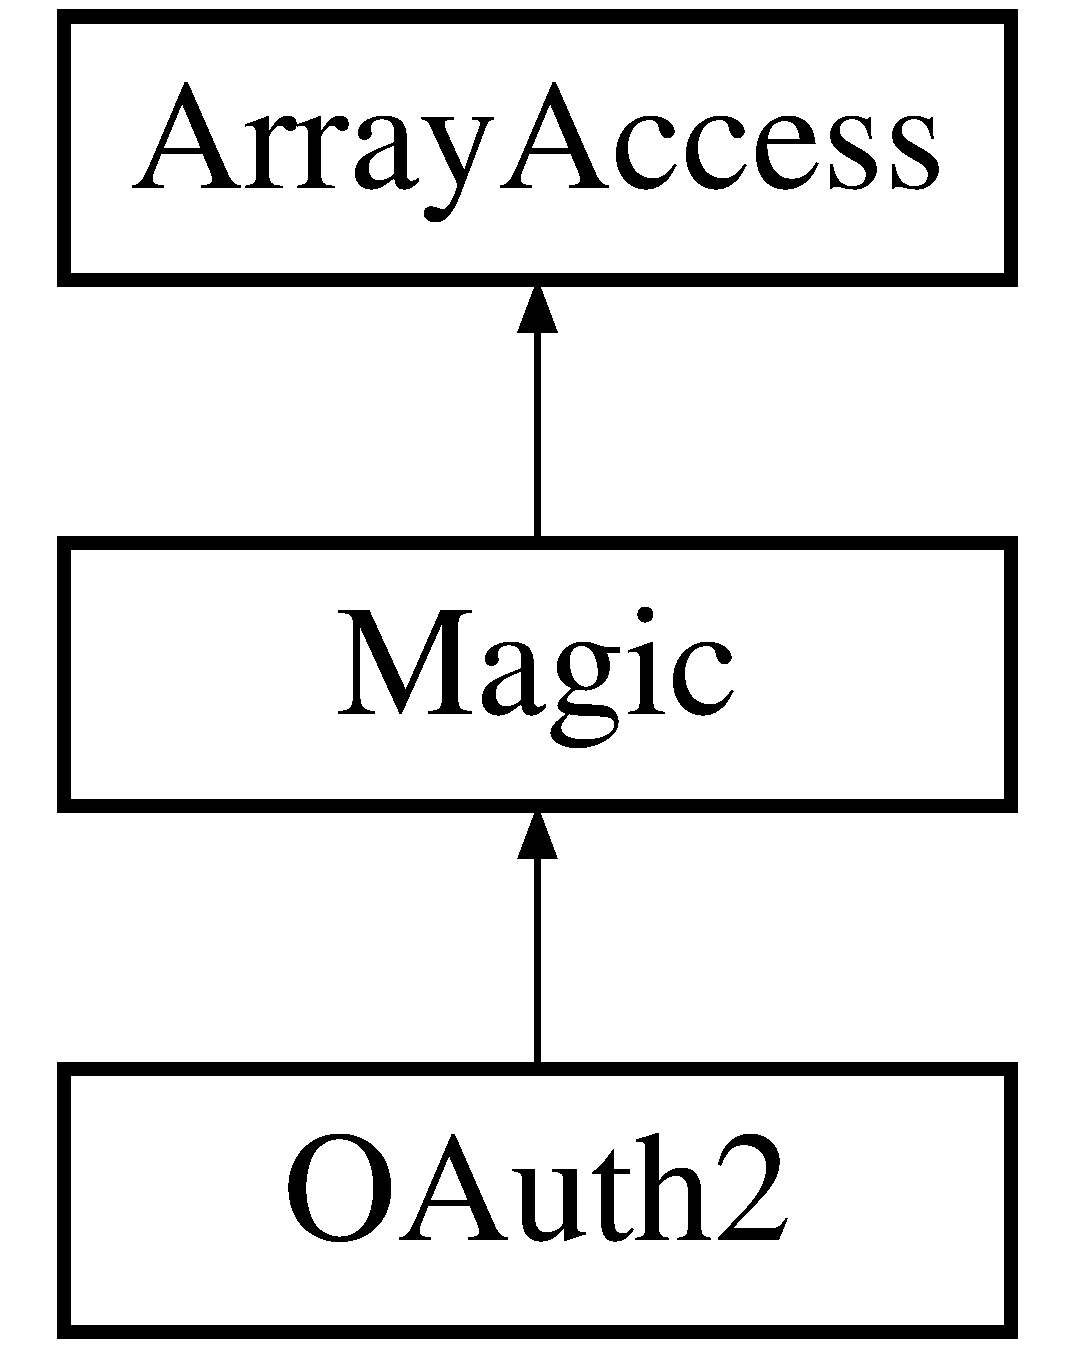
\includegraphics[height=3.000000cm]{class_web_1_1_o_auth2}
\end{center}
\end{figure}
\subsection*{Public Member Functions}
\begin{DoxyCompactItemize}
\item 
\hyperlink{class_web_1_1_o_auth2_a52f2721541169726269393c6eaaf8f53}{uri} (\$endpoint)
\item 
\hyperlink{class_web_1_1_o_auth2_ad75f56dfe168d5939f0c5b161d95d351}{request} (\$\hyperlink{class_web_1_1_o_auth2_a52f2721541169726269393c6eaaf8f53}{uri}, \$method, \$token=N\+U\+LL)
\item 
\hyperlink{class_web_1_1_o_auth2_a0520d136dfbea7d3360681b460d23a3c}{jwt} (\$token)
\item 
\hyperlink{class_web_1_1_o_auth2_ace1ae5be37bf26c172cc7ea4e1a65e26}{exists} (\$key)
\item 
\hyperlink{class_web_1_1_o_auth2_ac8d8012023e560c81f55a629022cb65a}{set} (\$key, \$val)
\item 
\& \hyperlink{class_web_1_1_o_auth2_ac3695923790b06917410e205068b8376}{get} (\$key)
\item 
\hyperlink{class_web_1_1_o_auth2_a3afe9e27ee9d208e19b23b9e5ba2689a}{clear} (\$key=N\+U\+LL)
\end{DoxyCompactItemize}
\subsection*{Protected Attributes}
\begin{DoxyCompactItemize}
\item 
\hypertarget{class_web_1_1_o_auth2_a67e94494731d99ed23b123e95175bc10}{}\label{class_web_1_1_o_auth2_a67e94494731d99ed23b123e95175bc10} 
\hyperlink{class_web_1_1_o_auth2_a67e94494731d99ed23b123e95175bc10}{\$args} =\mbox{[}$\,$\mbox{]}
\begin{DoxyCompactList}\small\item\em Scopes and claims. \end{DoxyCompactList}\end{DoxyCompactItemize}


\subsection{Detailed Description}
Lightweight \hyperlink{class_web_1_1_o_auth2}{O\+Auth2} client. 

Definition at line 26 of file oauth2.\+php.



\subsection{Member Function Documentation}
\hypertarget{class_web_1_1_o_auth2_a3afe9e27ee9d208e19b23b9e5ba2689a}{}\label{class_web_1_1_o_auth2_a3afe9e27ee9d208e19b23b9e5ba2689a} 
\index{Web\+::\+O\+Auth2@{Web\+::\+O\+Auth2}!clear@{clear}}
\index{clear@{clear}!Web\+::\+O\+Auth2@{Web\+::\+O\+Auth2}}
\subsubsection{\texorpdfstring{clear()}{clear()}}
{\footnotesize\ttfamily clear (\begin{DoxyParamCaption}\item[{}]{\$key = {\ttfamily NULL} }\end{DoxyParamCaption})}

Remove scope/claim \begin{DoxyReturn}{Returns}
N\+U\+LL 
\end{DoxyReturn}

\begin{DoxyParams}{Parameters}
{\em \$key} & \\
\hline
\end{DoxyParams}


Definition at line 126 of file oauth2.\+php.

\hypertarget{class_web_1_1_o_auth2_ace1ae5be37bf26c172cc7ea4e1a65e26}{}\label{class_web_1_1_o_auth2_ace1ae5be37bf26c172cc7ea4e1a65e26} 
\index{Web\+::\+O\+Auth2@{Web\+::\+O\+Auth2}!exists@{exists}}
\index{exists@{exists}!Web\+::\+O\+Auth2@{Web\+::\+O\+Auth2}}
\subsubsection{\texorpdfstring{exists()}{exists()}}
{\footnotesize\ttfamily exists (\begin{DoxyParamCaption}\item[{}]{\$key }\end{DoxyParamCaption})}

Return T\+R\+UE if scope/claim exists \begin{DoxyReturn}{Returns}
bool 
\end{DoxyReturn}

\begin{DoxyParams}{Parameters}
{\em \$key} & string \\
\hline
\end{DoxyParams}


Definition at line 94 of file oauth2.\+php.

\hypertarget{class_web_1_1_o_auth2_ac3695923790b06917410e205068b8376}{}\label{class_web_1_1_o_auth2_ac3695923790b06917410e205068b8376} 
\index{Web\+::\+O\+Auth2@{Web\+::\+O\+Auth2}!get@{get}}
\index{get@{get}!Web\+::\+O\+Auth2@{Web\+::\+O\+Auth2}}
\subsubsection{\texorpdfstring{get()}{get()}}
{\footnotesize\ttfamily \& get (\begin{DoxyParamCaption}\item[{}]{\$key }\end{DoxyParamCaption})}

Return value of scope/claim \begin{DoxyReturn}{Returns}
mixed 
\end{DoxyReturn}

\begin{DoxyParams}{Parameters}
{\em \$key} & string \\
\hline
\end{DoxyParams}


Definition at line 113 of file oauth2.\+php.

\hypertarget{class_web_1_1_o_auth2_a0520d136dfbea7d3360681b460d23a3c}{}\label{class_web_1_1_o_auth2_a0520d136dfbea7d3360681b460d23a3c} 
\index{Web\+::\+O\+Auth2@{Web\+::\+O\+Auth2}!jwt@{jwt}}
\index{jwt@{jwt}!Web\+::\+O\+Auth2@{Web\+::\+O\+Auth2}}
\subsubsection{\texorpdfstring{jwt()}{jwt()}}
{\footnotesize\ttfamily jwt (\begin{DoxyParamCaption}\item[{}]{\$token }\end{DoxyParamCaption})}

Parse J\+S\+ON \hyperlink{class_web}{Web} token \begin{DoxyReturn}{Returns}
array 
\end{DoxyReturn}

\begin{DoxyParams}{Parameters}
{\em \$token} & string \\
\hline
\end{DoxyParams}


Definition at line 76 of file oauth2.\+php.

\hypertarget{class_web_1_1_o_auth2_ad75f56dfe168d5939f0c5b161d95d351}{}\label{class_web_1_1_o_auth2_ad75f56dfe168d5939f0c5b161d95d351} 
\index{Web\+::\+O\+Auth2@{Web\+::\+O\+Auth2}!request@{request}}
\index{request@{request}!Web\+::\+O\+Auth2@{Web\+::\+O\+Auth2}}
\subsubsection{\texorpdfstring{request()}{request()}}
{\footnotesize\ttfamily request (\begin{DoxyParamCaption}\item[{}]{\$uri,  }\item[{}]{\$method,  }\item[{}]{\$token = {\ttfamily NULL} }\end{DoxyParamCaption})}

Send request to A\+P\+I/token endpoint \begin{DoxyReturn}{Returns}
string$\vert$\+F\+A\+L\+SE 
\end{DoxyReturn}

\begin{DoxyParams}{Parameters}
{\em \$uri} & string \\
\hline
{\em \$method} & string \\
\hline
{\em \$token} & array \\
\hline
\end{DoxyParams}


Definition at line 48 of file oauth2.\+php.

\hypertarget{class_web_1_1_o_auth2_ac8d8012023e560c81f55a629022cb65a}{}\label{class_web_1_1_o_auth2_ac8d8012023e560c81f55a629022cb65a} 
\index{Web\+::\+O\+Auth2@{Web\+::\+O\+Auth2}!set@{set}}
\index{set@{set}!Web\+::\+O\+Auth2@{Web\+::\+O\+Auth2}}
\subsubsection{\texorpdfstring{set()}{set()}}
{\footnotesize\ttfamily set (\begin{DoxyParamCaption}\item[{}]{\$key,  }\item[{}]{\$val }\end{DoxyParamCaption})}

Bind value to scope/claim \begin{DoxyReturn}{Returns}
string 
\end{DoxyReturn}

\begin{DoxyParams}{Parameters}
{\em \$key} & string \\
\hline
{\em \$val} & string \\
\hline
\end{DoxyParams}


Definition at line 104 of file oauth2.\+php.

\hypertarget{class_web_1_1_o_auth2_a52f2721541169726269393c6eaaf8f53}{}\label{class_web_1_1_o_auth2_a52f2721541169726269393c6eaaf8f53} 
\index{Web\+::\+O\+Auth2@{Web\+::\+O\+Auth2}!uri@{uri}}
\index{uri@{uri}!Web\+::\+O\+Auth2@{Web\+::\+O\+Auth2}}
\subsubsection{\texorpdfstring{uri()}{uri()}}
{\footnotesize\ttfamily uri (\begin{DoxyParamCaption}\item[{}]{\$endpoint }\end{DoxyParamCaption})}

Return \hyperlink{class_web_1_1_o_auth2}{O\+Auth2} authentication U\+RI \begin{DoxyReturn}{Returns}
string 
\end{DoxyReturn}

\begin{DoxyParams}{Parameters}
{\em \$endpoint} & string \\
\hline
\end{DoxyParams}


Definition at line 37 of file oauth2.\+php.



The documentation for this class was generated from the following file\+:\begin{DoxyCompactItemize}
\item 
/\+Users/aplennevaux/\+G\+I\+T\+H\+U\+B/\+Visionary-\/website/src/vendor/bcosca/fatfree/lib/web/oauth2.\+php\end{DoxyCompactItemize}

\hypertarget{class_web_1_1_open_i_d}{}\section{Open\+ID Class Reference}
\label{class_web_1_1_open_i_d}\index{Open\+ID@{Open\+ID}}


\hyperlink{class_web_1_1_open_i_d}{Open\+ID} consumer.  


Inheritance diagram for Open\+ID\+:\begin{figure}[H]
\begin{center}
\leavevmode
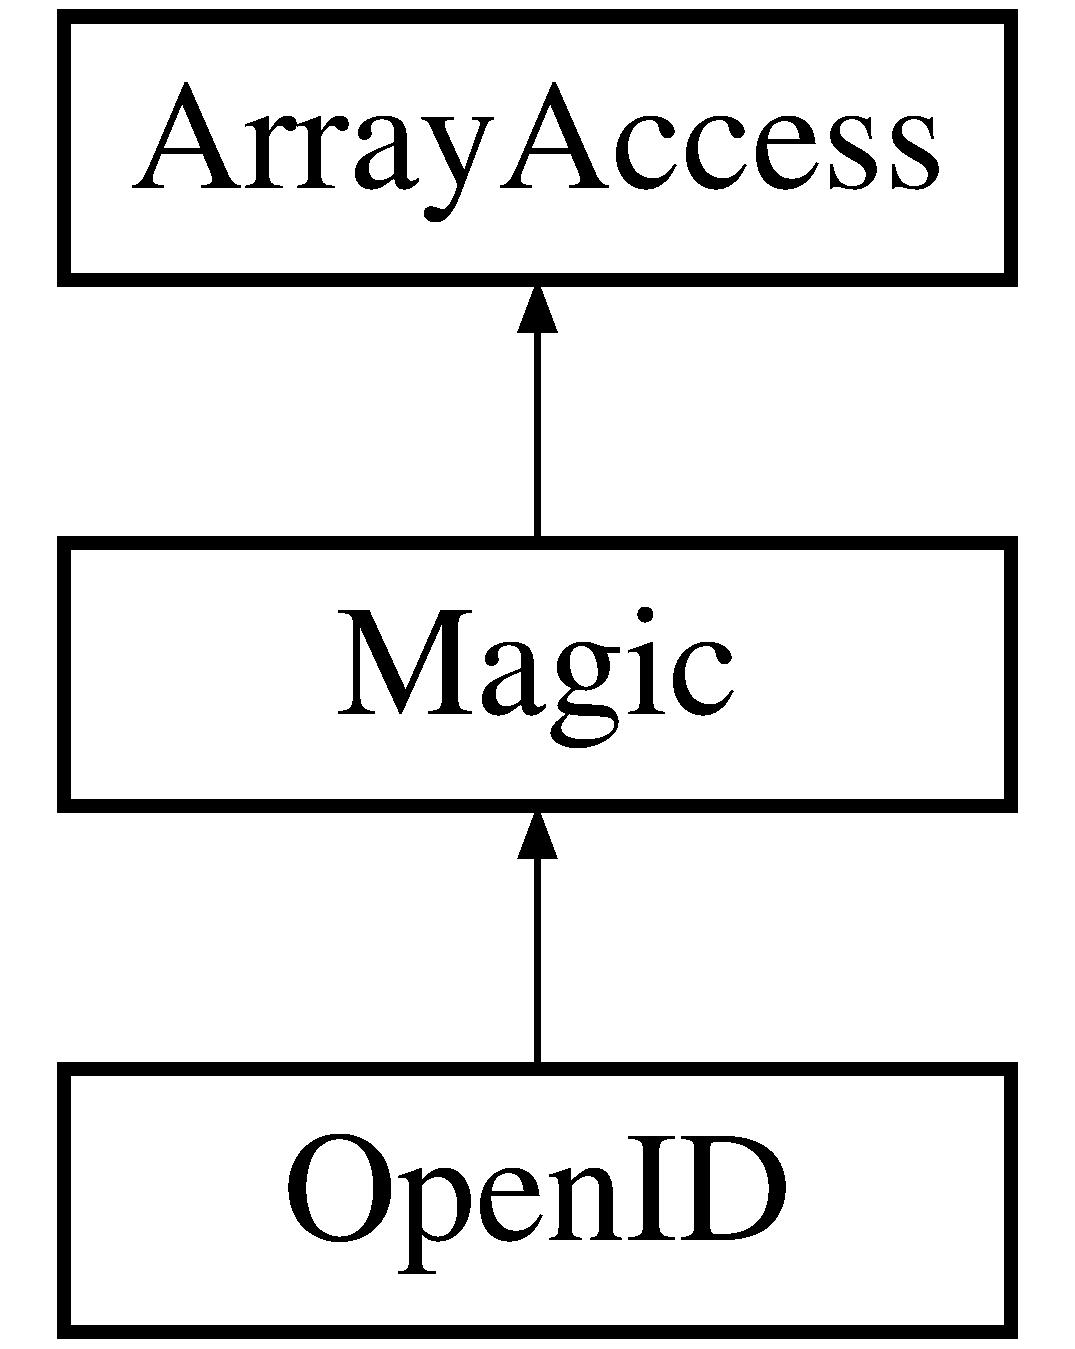
\includegraphics[height=3.000000cm]{class_web_1_1_open_i_d}
\end{center}
\end{figure}
\subsection*{Public Member Functions}
\begin{DoxyCompactItemize}
\item 
\hyperlink{class_web_1_1_open_i_d_a83c8bf3d9d47536f727fce44c00de4f0}{auth} (\$proxy=N\+U\+LL, \$attr=\mbox{[}$\,$\mbox{]}, array \$reqd=N\+U\+LL)
\item 
\hyperlink{class_web_1_1_open_i_d_a5d29540442d0e302ca0916620ad2bc17}{verified} (\$proxy=N\+U\+LL)
\item 
\hyperlink{class_web_1_1_open_i_d_a1e3f1bea94184e9ba901797124266e96}{response} ()
\item 
\hyperlink{class_web_1_1_open_i_d_ace1ae5be37bf26c172cc7ea4e1a65e26}{exists} (\$key)
\item 
\hyperlink{class_web_1_1_open_i_d_ac8d8012023e560c81f55a629022cb65a}{set} (\$key, \$val)
\item 
\& \hyperlink{class_web_1_1_open_i_d_ac3695923790b06917410e205068b8376}{get} (\$key)
\item 
\hyperlink{class_web_1_1_open_i_d_a10a949ef75de6c82c98ac555f371ba83}{clear} (\$key)
\end{DoxyCompactItemize}
\subsection*{Data Fields}
\begin{DoxyCompactItemize}
\item 
\hypertarget{class_web_1_1_open_i_d_a67e94494731d99ed23b123e95175bc10}{}\label{class_web_1_1_open_i_d_a67e94494731d99ed23b123e95175bc10} 
\hyperlink{class_web_1_1_open_i_d_a67e94494731d99ed23b123e95175bc10}{\$args} =\mbox{[}$\,$\mbox{]}
\begin{DoxyCompactList}\small\item\em H\+T\+TP request parameters. \end{DoxyCompactList}\end{DoxyCompactItemize}
\subsection*{Protected Member Functions}
\begin{DoxyCompactItemize}
\item 
\hyperlink{class_web_1_1_open_i_d_a8fe09384f979cc36cabfcc675e1de1d7}{discover} (\$proxy)
\end{DoxyCompactItemize}
\subsection*{Protected Attributes}
\begin{DoxyCompactItemize}
\item 
\hypertarget{class_web_1_1_open_i_d_acf215f34a917d014776ce684a9ee8909}{}\label{class_web_1_1_open_i_d_acf215f34a917d014776ce684a9ee8909} 
\hyperlink{class_web_1_1_open_i_d_acf215f34a917d014776ce684a9ee8909}{\$url}
\begin{DoxyCompactList}\small\item\em \hyperlink{class_web_1_1_open_i_d}{Open\+ID} provider endpoint U\+RL. \end{DoxyCompactList}\end{DoxyCompactItemize}


\subsection{Detailed Description}
\hyperlink{class_web_1_1_open_i_d}{Open\+ID} consumer. 

Definition at line 26 of file openid.\+php.



\subsection{Member Function Documentation}
\hypertarget{class_web_1_1_open_i_d_a83c8bf3d9d47536f727fce44c00de4f0}{}\label{class_web_1_1_open_i_d_a83c8bf3d9d47536f727fce44c00de4f0} 
\index{Web\+::\+Open\+ID@{Web\+::\+Open\+ID}!auth@{auth}}
\index{auth@{auth}!Web\+::\+Open\+ID@{Web\+::\+Open\+ID}}
\subsubsection{\texorpdfstring{auth()}{auth()}}
{\footnotesize\ttfamily auth (\begin{DoxyParamCaption}\item[{}]{\$proxy = {\ttfamily NULL},  }\item[{}]{\$attr = {\ttfamily \mbox{[}\mbox{]}},  }\item[{array}]{\$reqd = {\ttfamily NULL} }\end{DoxyParamCaption})}

Initiate \hyperlink{class_web_1_1_open_i_d}{Open\+ID} authentication sequence; Return F\+A\+L\+SE on failure or redirect to \hyperlink{class_web_1_1_open_i_d}{Open\+ID} provider U\+RL \begin{DoxyReturn}{Returns}
bool 
\end{DoxyReturn}

\begin{DoxyParams}{Parameters}
{\em \$proxy} & string \\
\hline
{\em \$attr} & array \\
\hline
{\em \$reqd} & string$\vert$array \\
\hline
\end{DoxyParams}


Definition at line 144 of file openid.\+php.

\hypertarget{class_web_1_1_open_i_d_a10a949ef75de6c82c98ac555f371ba83}{}\label{class_web_1_1_open_i_d_a10a949ef75de6c82c98ac555f371ba83} 
\index{Web\+::\+Open\+ID@{Web\+::\+Open\+ID}!clear@{clear}}
\index{clear@{clear}!Web\+::\+Open\+ID@{Web\+::\+Open\+ID}}
\subsubsection{\texorpdfstring{clear()}{clear()}}
{\footnotesize\ttfamily clear (\begin{DoxyParamCaption}\item[{}]{\$key }\end{DoxyParamCaption})}

Remove \hyperlink{class_web_1_1_open_i_d}{Open\+ID} request parameter \begin{DoxyReturn}{Returns}
N\+U\+LL 
\end{DoxyReturn}

\begin{DoxyParams}{Parameters}
{\em \$key} & \\
\hline
\end{DoxyParams}


Definition at line 244 of file openid.\+php.

\hypertarget{class_web_1_1_open_i_d_a8fe09384f979cc36cabfcc675e1de1d7}{}\label{class_web_1_1_open_i_d_a8fe09384f979cc36cabfcc675e1de1d7} 
\index{Web\+::\+Open\+ID@{Web\+::\+Open\+ID}!discover@{discover}}
\index{discover@{discover}!Web\+::\+Open\+ID@{Web\+::\+Open\+ID}}
\subsubsection{\texorpdfstring{discover()}{discover()}}
{\footnotesize\ttfamily discover (\begin{DoxyParamCaption}\item[{}]{\$proxy }\end{DoxyParamCaption})\hspace{0.3cm}{\ttfamily [protected]}}

Determine \hyperlink{class_web_1_1_open_i_d}{Open\+ID} provider \begin{DoxyReturn}{Returns}
string$\vert$\+F\+A\+L\+SE 
\end{DoxyReturn}

\begin{DoxyParams}{Parameters}
{\em \$proxy} & string \\
\hline
\end{DoxyParams}


Definition at line 39 of file openid.\+php.

\hypertarget{class_web_1_1_open_i_d_ace1ae5be37bf26c172cc7ea4e1a65e26}{}\label{class_web_1_1_open_i_d_ace1ae5be37bf26c172cc7ea4e1a65e26} 
\index{Web\+::\+Open\+ID@{Web\+::\+Open\+ID}!exists@{exists}}
\index{exists@{exists}!Web\+::\+Open\+ID@{Web\+::\+Open\+ID}}
\subsubsection{\texorpdfstring{exists()}{exists()}}
{\footnotesize\ttfamily exists (\begin{DoxyParamCaption}\item[{}]{\$key }\end{DoxyParamCaption})}

Return T\+R\+UE if \hyperlink{class_web_1_1_open_i_d}{Open\+ID} request parameter exists \begin{DoxyReturn}{Returns}
bool 
\end{DoxyReturn}

\begin{DoxyParams}{Parameters}
{\em \$key} & string \\
\hline
\end{DoxyParams}


Definition at line 212 of file openid.\+php.

\hypertarget{class_web_1_1_open_i_d_ac3695923790b06917410e205068b8376}{}\label{class_web_1_1_open_i_d_ac3695923790b06917410e205068b8376} 
\index{Web\+::\+Open\+ID@{Web\+::\+Open\+ID}!get@{get}}
\index{get@{get}!Web\+::\+Open\+ID@{Web\+::\+Open\+ID}}
\subsubsection{\texorpdfstring{get()}{get()}}
{\footnotesize\ttfamily \& get (\begin{DoxyParamCaption}\item[{}]{\$key }\end{DoxyParamCaption})}

Return value of \hyperlink{class_web_1_1_open_i_d}{Open\+ID} request parameter \begin{DoxyReturn}{Returns}
mixed 
\end{DoxyReturn}

\begin{DoxyParams}{Parameters}
{\em \$key} & string \\
\hline
\end{DoxyParams}


Definition at line 231 of file openid.\+php.

\hypertarget{class_web_1_1_open_i_d_a1e3f1bea94184e9ba901797124266e96}{}\label{class_web_1_1_open_i_d_a1e3f1bea94184e9ba901797124266e96} 
\index{Web\+::\+Open\+ID@{Web\+::\+Open\+ID}!response@{response}}
\index{response@{response}!Web\+::\+Open\+ID@{Web\+::\+Open\+ID}}
\subsubsection{\texorpdfstring{response()}{response()}}
{\footnotesize\ttfamily response (\begin{DoxyParamCaption}{ }\end{DoxyParamCaption})}

Return \hyperlink{class_web_1_1_open_i_d}{Open\+ID} response fields \begin{DoxyReturn}{Returns}
array 
\end{DoxyReturn}


Definition at line 203 of file openid.\+php.

\hypertarget{class_web_1_1_open_i_d_ac8d8012023e560c81f55a629022cb65a}{}\label{class_web_1_1_open_i_d_ac8d8012023e560c81f55a629022cb65a} 
\index{Web\+::\+Open\+ID@{Web\+::\+Open\+ID}!set@{set}}
\index{set@{set}!Web\+::\+Open\+ID@{Web\+::\+Open\+ID}}
\subsubsection{\texorpdfstring{set()}{set()}}
{\footnotesize\ttfamily set (\begin{DoxyParamCaption}\item[{}]{\$key,  }\item[{}]{\$val }\end{DoxyParamCaption})}

Bind value to \hyperlink{class_web_1_1_open_i_d}{Open\+ID} request parameter \begin{DoxyReturn}{Returns}
string 
\end{DoxyReturn}

\begin{DoxyParams}{Parameters}
{\em \$key} & string \\
\hline
{\em \$val} & string \\
\hline
\end{DoxyParams}


Definition at line 222 of file openid.\+php.

\hypertarget{class_web_1_1_open_i_d_a5d29540442d0e302ca0916620ad2bc17}{}\label{class_web_1_1_open_i_d_a5d29540442d0e302ca0916620ad2bc17} 
\index{Web\+::\+Open\+ID@{Web\+::\+Open\+ID}!verified@{verified}}
\index{verified@{verified}!Web\+::\+Open\+ID@{Web\+::\+Open\+ID}}
\subsubsection{\texorpdfstring{verified()}{verified()}}
{\footnotesize\ttfamily verified (\begin{DoxyParamCaption}\item[{}]{\$proxy = {\ttfamily NULL} }\end{DoxyParamCaption})}

Return T\+R\+UE if \hyperlink{class_web_1_1_open_i_d}{Open\+ID} verification was successful \begin{DoxyReturn}{Returns}
bool 
\end{DoxyReturn}

\begin{DoxyParams}{Parameters}
{\em \$proxy} & string \\
\hline
\end{DoxyParams}


Definition at line 174 of file openid.\+php.



The documentation for this class was generated from the following file\+:\begin{DoxyCompactItemize}
\item 
/\+Users/aplennevaux/\+G\+I\+T\+H\+U\+B/\+Visionary-\/website/src/vendor/bcosca/fatfree/lib/web/openid.\+php\end{DoxyCompactItemize}

\hypertarget{class_web_1_1_pingback}{}\section{Pingback Class Reference}
\label{class_web_1_1_pingback}\index{Pingback@{Pingback}}


\hyperlink{class_web_1_1_pingback}{Pingback} 1.\+0 protocol (client and server) implementation.  


Inheritance diagram for Pingback\+:\begin{figure}[H]
\begin{center}
\leavevmode
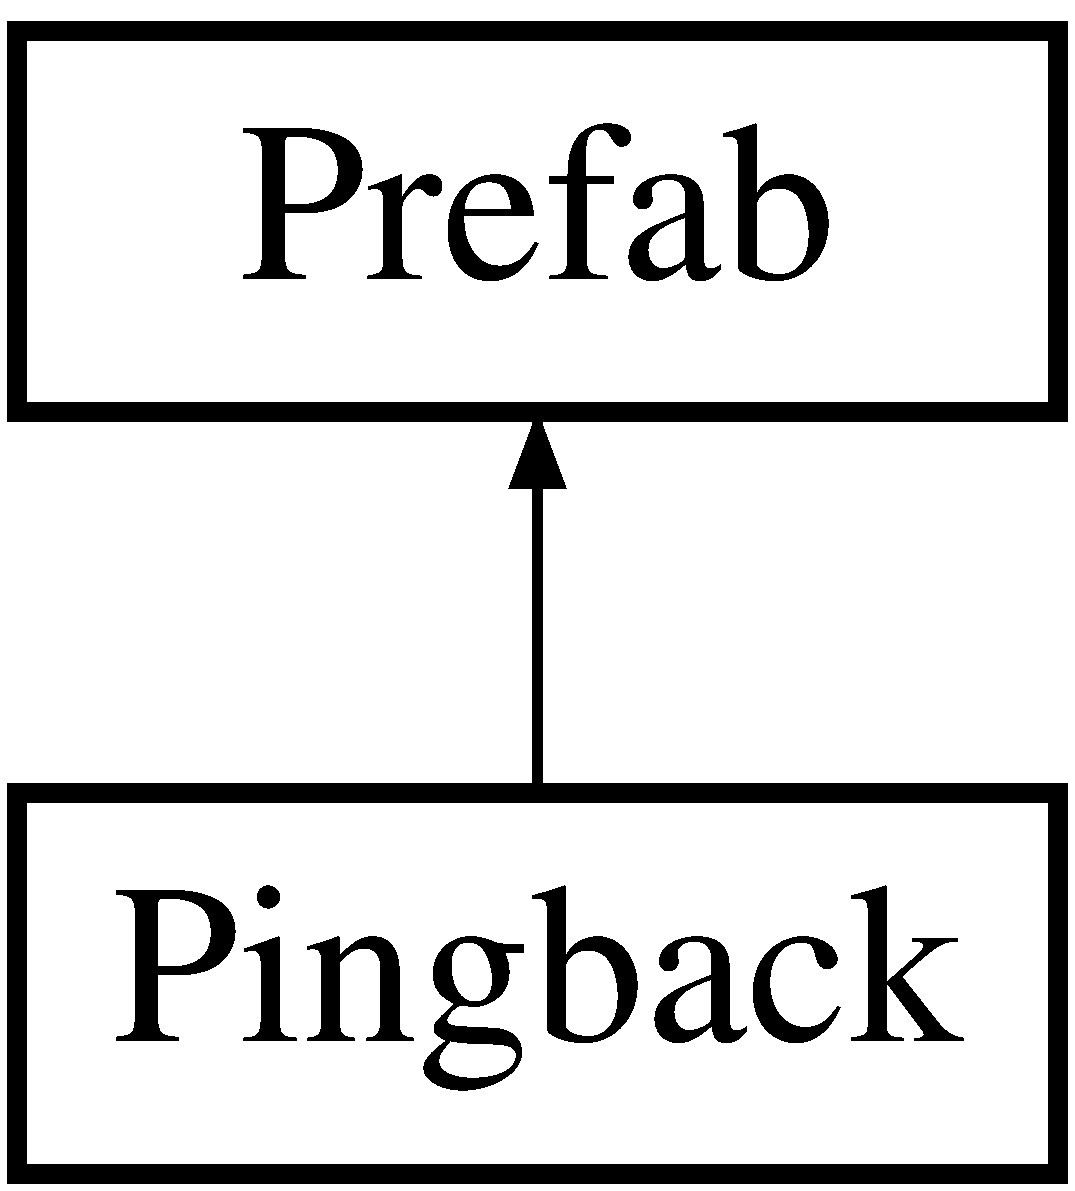
\includegraphics[height=2.000000cm]{class_web_1_1_pingback}
\end{center}
\end{figure}
\subsection*{Public Member Functions}
\begin{DoxyCompactItemize}
\item 
\hyperlink{class_web_1_1_pingback_af2f57c4ad56194df3b169d4993d49dbb}{inspect} (\$source)
\item 
\hyperlink{class_web_1_1_pingback_aa1f607b468feb8edba01ef661f980294}{listen} (\$func, \$path=N\+U\+LL)
\item 
\hyperlink{class_web_1_1_pingback_a5e06d9b7f0033278f40a41d081efbe71}{log} ()
\item 
\hyperlink{class_web_1_1_pingback_a095c5d389db211932136b53f25f39685}{\+\_\+\+\_\+construct} ()
\end{DoxyCompactItemize}
\subsection*{Protected Member Functions}
\begin{DoxyCompactItemize}
\item 
\hyperlink{class_web_1_1_pingback_a40d5adaa4e43f4c875ad081d7118ce4e}{enabled} (\$url)
\end{DoxyCompactItemize}
\subsection*{Protected Attributes}
\begin{DoxyCompactItemize}
\item 
\hypertarget{class_web_1_1_pingback_a9a2cf15a653aee8be437f7ae474cd494}{}\label{class_web_1_1_pingback_a9a2cf15a653aee8be437f7ae474cd494} 
\hyperlink{class_web_1_1_pingback_a9a2cf15a653aee8be437f7ae474cd494}{\$log}
\begin{DoxyCompactList}\small\item\em Transaction history. \end{DoxyCompactList}\end{DoxyCompactItemize}
\subsection*{Additional Inherited Members}


\subsection{Detailed Description}
\hyperlink{class_web_1_1_pingback}{Pingback} 1.\+0 protocol (client and server) implementation. 

Definition at line 26 of file pingback.\+php.



\subsection{Constructor \& Destructor Documentation}
\hypertarget{class_web_1_1_pingback_a095c5d389db211932136b53f25f39685}{}\label{class_web_1_1_pingback_a095c5d389db211932136b53f25f39685} 
\index{Web\+::\+Pingback@{Web\+::\+Pingback}!\+\_\+\+\_\+construct@{\+\_\+\+\_\+construct}}
\index{\+\_\+\+\_\+construct@{\+\_\+\+\_\+construct}!Web\+::\+Pingback@{Web\+::\+Pingback}}
\subsubsection{\texorpdfstring{\+\_\+\+\_\+construct()}{\_\_construct()}}
{\footnotesize\ttfamily \+\_\+\+\_\+construct (\begin{DoxyParamCaption}{ }\end{DoxyParamCaption})}

Instantiate class \begin{DoxyReturn}{Returns}
object 
\end{DoxyReturn}


Definition at line 171 of file pingback.\+php.



\subsection{Member Function Documentation}
\hypertarget{class_web_1_1_pingback_a40d5adaa4e43f4c875ad081d7118ce4e}{}\label{class_web_1_1_pingback_a40d5adaa4e43f4c875ad081d7118ce4e} 
\index{Web\+::\+Pingback@{Web\+::\+Pingback}!enabled@{enabled}}
\index{enabled@{enabled}!Web\+::\+Pingback@{Web\+::\+Pingback}}
\subsubsection{\texorpdfstring{enabled()}{enabled()}}
{\footnotesize\ttfamily enabled (\begin{DoxyParamCaption}\item[{}]{\$url }\end{DoxyParamCaption})\hspace{0.3cm}{\ttfamily [protected]}}

Return T\+R\+UE if U\+RL points to a pingback-\/enabled resource \begin{DoxyReturn}{Returns}
bool 
\end{DoxyReturn}

\begin{DoxyParams}{Parameters}
{\em \$url} & \\
\hline
\end{DoxyParams}


Definition at line 37 of file pingback.\+php.

\hypertarget{class_web_1_1_pingback_af2f57c4ad56194df3b169d4993d49dbb}{}\label{class_web_1_1_pingback_af2f57c4ad56194df3b169d4993d49dbb} 
\index{Web\+::\+Pingback@{Web\+::\+Pingback}!inspect@{inspect}}
\index{inspect@{inspect}!Web\+::\+Pingback@{Web\+::\+Pingback}}
\subsubsection{\texorpdfstring{inspect()}{inspect()}}
{\footnotesize\ttfamily inspect (\begin{DoxyParamCaption}\item[{}]{\$source }\end{DoxyParamCaption})}

Load local page contents, parse H\+T\+ML anchor tags, find permalinks, and send X\+M\+L-\/\+R\+PC calls to corresponding pingback servers \begin{DoxyReturn}{Returns}
N\+U\+LL 
\end{DoxyReturn}

\begin{DoxyParams}{Parameters}
{\em \$source} & string \\
\hline
\end{DoxyParams}


Definition at line 64 of file pingback.\+php.

\hypertarget{class_web_1_1_pingback_aa1f607b468feb8edba01ef661f980294}{}\label{class_web_1_1_pingback_aa1f607b468feb8edba01ef661f980294} 
\index{Web\+::\+Pingback@{Web\+::\+Pingback}!listen@{listen}}
\index{listen@{listen}!Web\+::\+Pingback@{Web\+::\+Pingback}}
\subsubsection{\texorpdfstring{listen()}{listen()}}
{\footnotesize\ttfamily listen (\begin{DoxyParamCaption}\item[{}]{\$func,  }\item[{}]{\$path = {\ttfamily NULL} }\end{DoxyParamCaption})}

Receive ping, check if local page is pingback-\/enabled, verify source contents, and return X\+M\+L-\/\+R\+PC response \begin{DoxyReturn}{Returns}
string 
\end{DoxyReturn}

\begin{DoxyParams}{Parameters}
{\em \$func} & callback \\
\hline
{\em \$path} & string \\
\hline
\end{DoxyParams}


Definition at line 110 of file pingback.\+php.

\hypertarget{class_web_1_1_pingback_a5e06d9b7f0033278f40a41d081efbe71}{}\label{class_web_1_1_pingback_a5e06d9b7f0033278f40a41d081efbe71} 
\index{Web\+::\+Pingback@{Web\+::\+Pingback}!log@{log}}
\index{log@{log}!Web\+::\+Pingback@{Web\+::\+Pingback}}
\subsubsection{\texorpdfstring{log()}{log()}}
{\footnotesize\ttfamily log (\begin{DoxyParamCaption}{ }\end{DoxyParamCaption})}

Return transaction history \begin{DoxyReturn}{Returns}
string 
\end{DoxyReturn}


Definition at line 163 of file pingback.\+php.



The documentation for this class was generated from the following file\+:\begin{DoxyCompactItemize}
\item 
/\+Users/aplennevaux/\+G\+I\+T\+H\+U\+B/\+Visionary-\/website/src/vendor/bcosca/fatfree/lib/web/pingback.\+php\end{DoxyCompactItemize}

\hypertarget{class_prefab}{}\section{Prefab Class Reference}
\label{class_prefab}\index{Prefab@{Prefab}}


Factory class for single-\/instance objects.  


Inheritance diagram for Prefab\+:\begin{figure}[H]
\begin{center}
\leavevmode
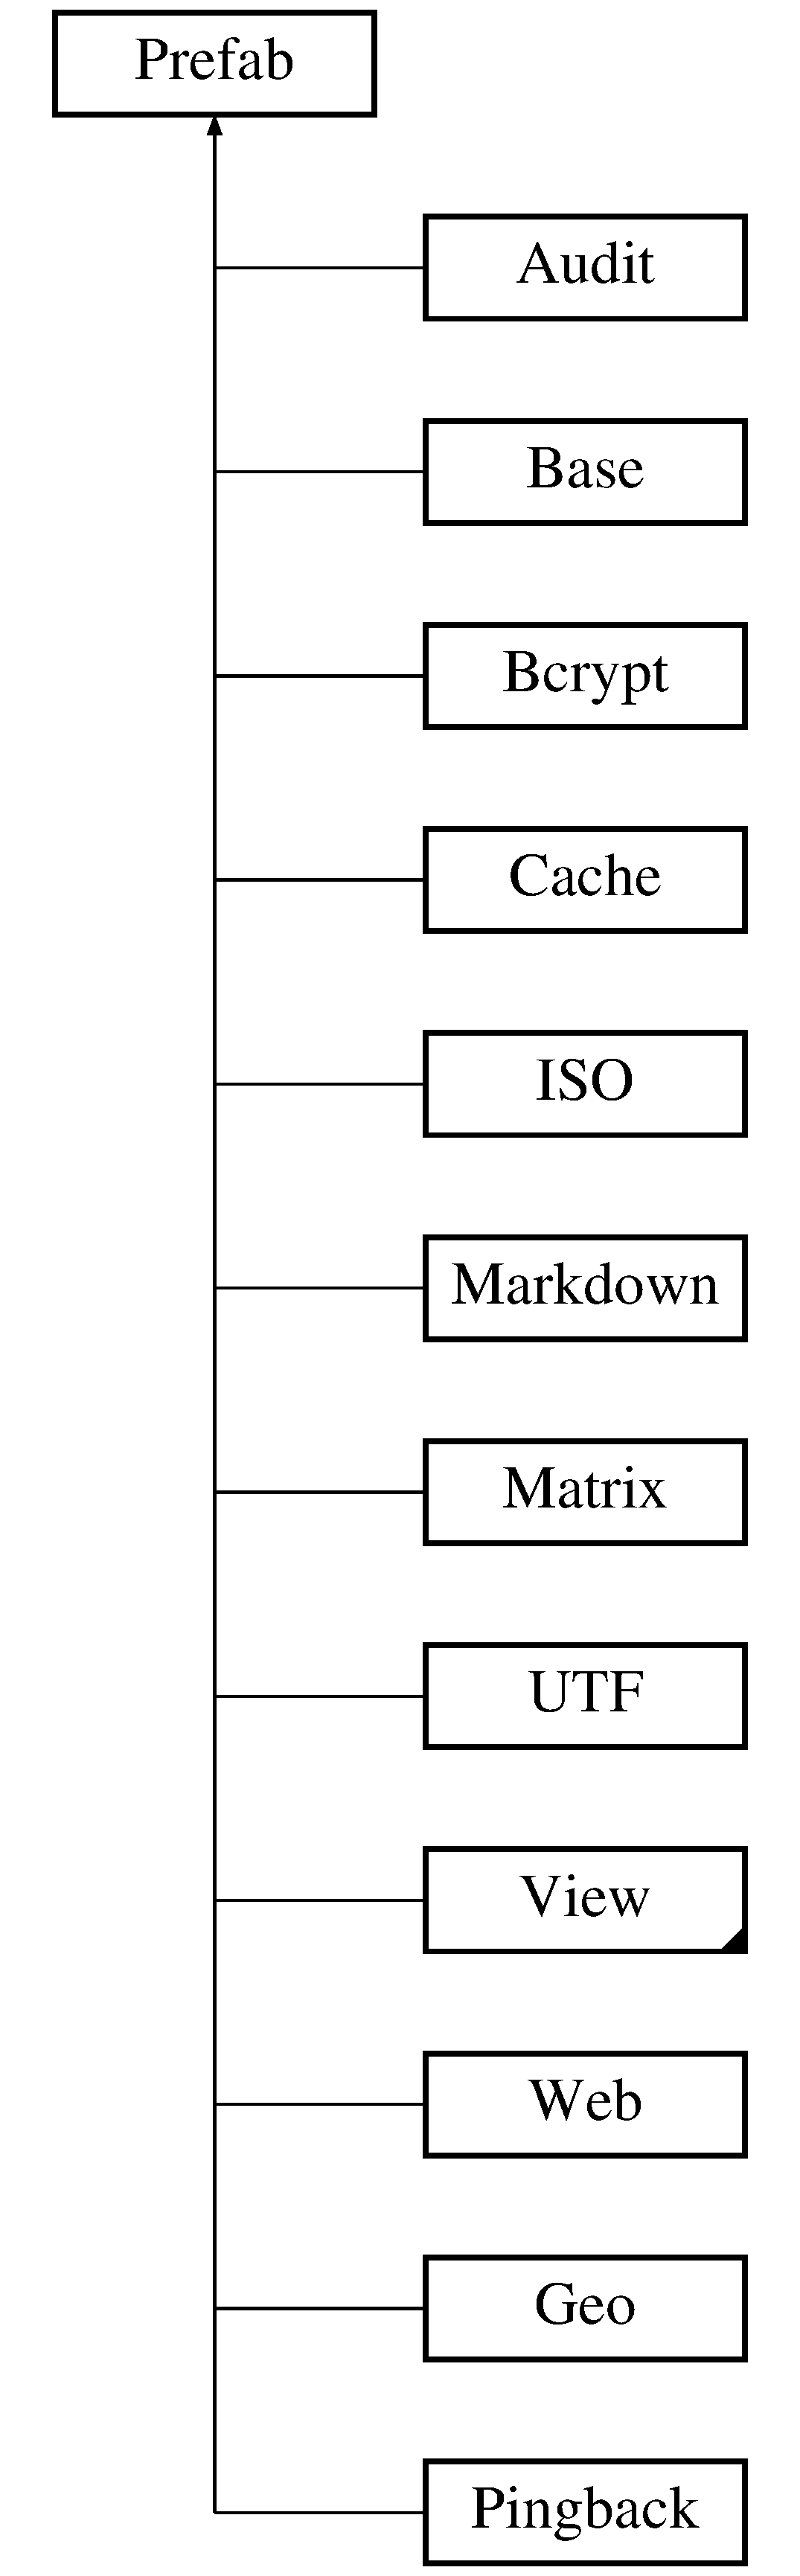
\includegraphics[height=12.000000cm]{class_prefab}
\end{center}
\end{figure}
\subsection*{Static Public Member Functions}
\begin{DoxyCompactItemize}
\item 
static \hyperlink{class_prefab_a0deb004950b8dc4f51836316fd19c111}{instance} ()
\end{DoxyCompactItemize}


\subsection{Detailed Description}
Factory class for single-\/instance objects. 

Definition at line 24 of file base.\+php.



\subsection{Member Function Documentation}
\hypertarget{class_prefab_a0deb004950b8dc4f51836316fd19c111}{}\label{class_prefab_a0deb004950b8dc4f51836316fd19c111} 
\index{Prefab@{Prefab}!instance@{instance}}
\index{instance@{instance}!Prefab@{Prefab}}
\subsubsection{\texorpdfstring{instance()}{instance()}}
{\footnotesize\ttfamily static instance (\begin{DoxyParamCaption}{ }\end{DoxyParamCaption})\hspace{0.3cm}{\ttfamily [static]}}

Return class instance \begin{DoxyReturn}{Returns}
static 
\end{DoxyReturn}


Definition at line 30 of file base.\+php.



The documentation for this class was generated from the following file\+:\begin{DoxyCompactItemize}
\item 
/\+Users/aplennevaux/\+G\+I\+T\+H\+U\+B/\+Visionary-\/website/src/vendor/bcosca/fatfree/lib/base.\+php\end{DoxyCompactItemize}

\hypertarget{class_preview}{}\section{Preview Class Reference}
\label{class_preview}\index{Preview@{Preview}}


Lightweight template engine.  


Inheritance diagram for Preview\+:\begin{figure}[H]
\begin{center}
\leavevmode
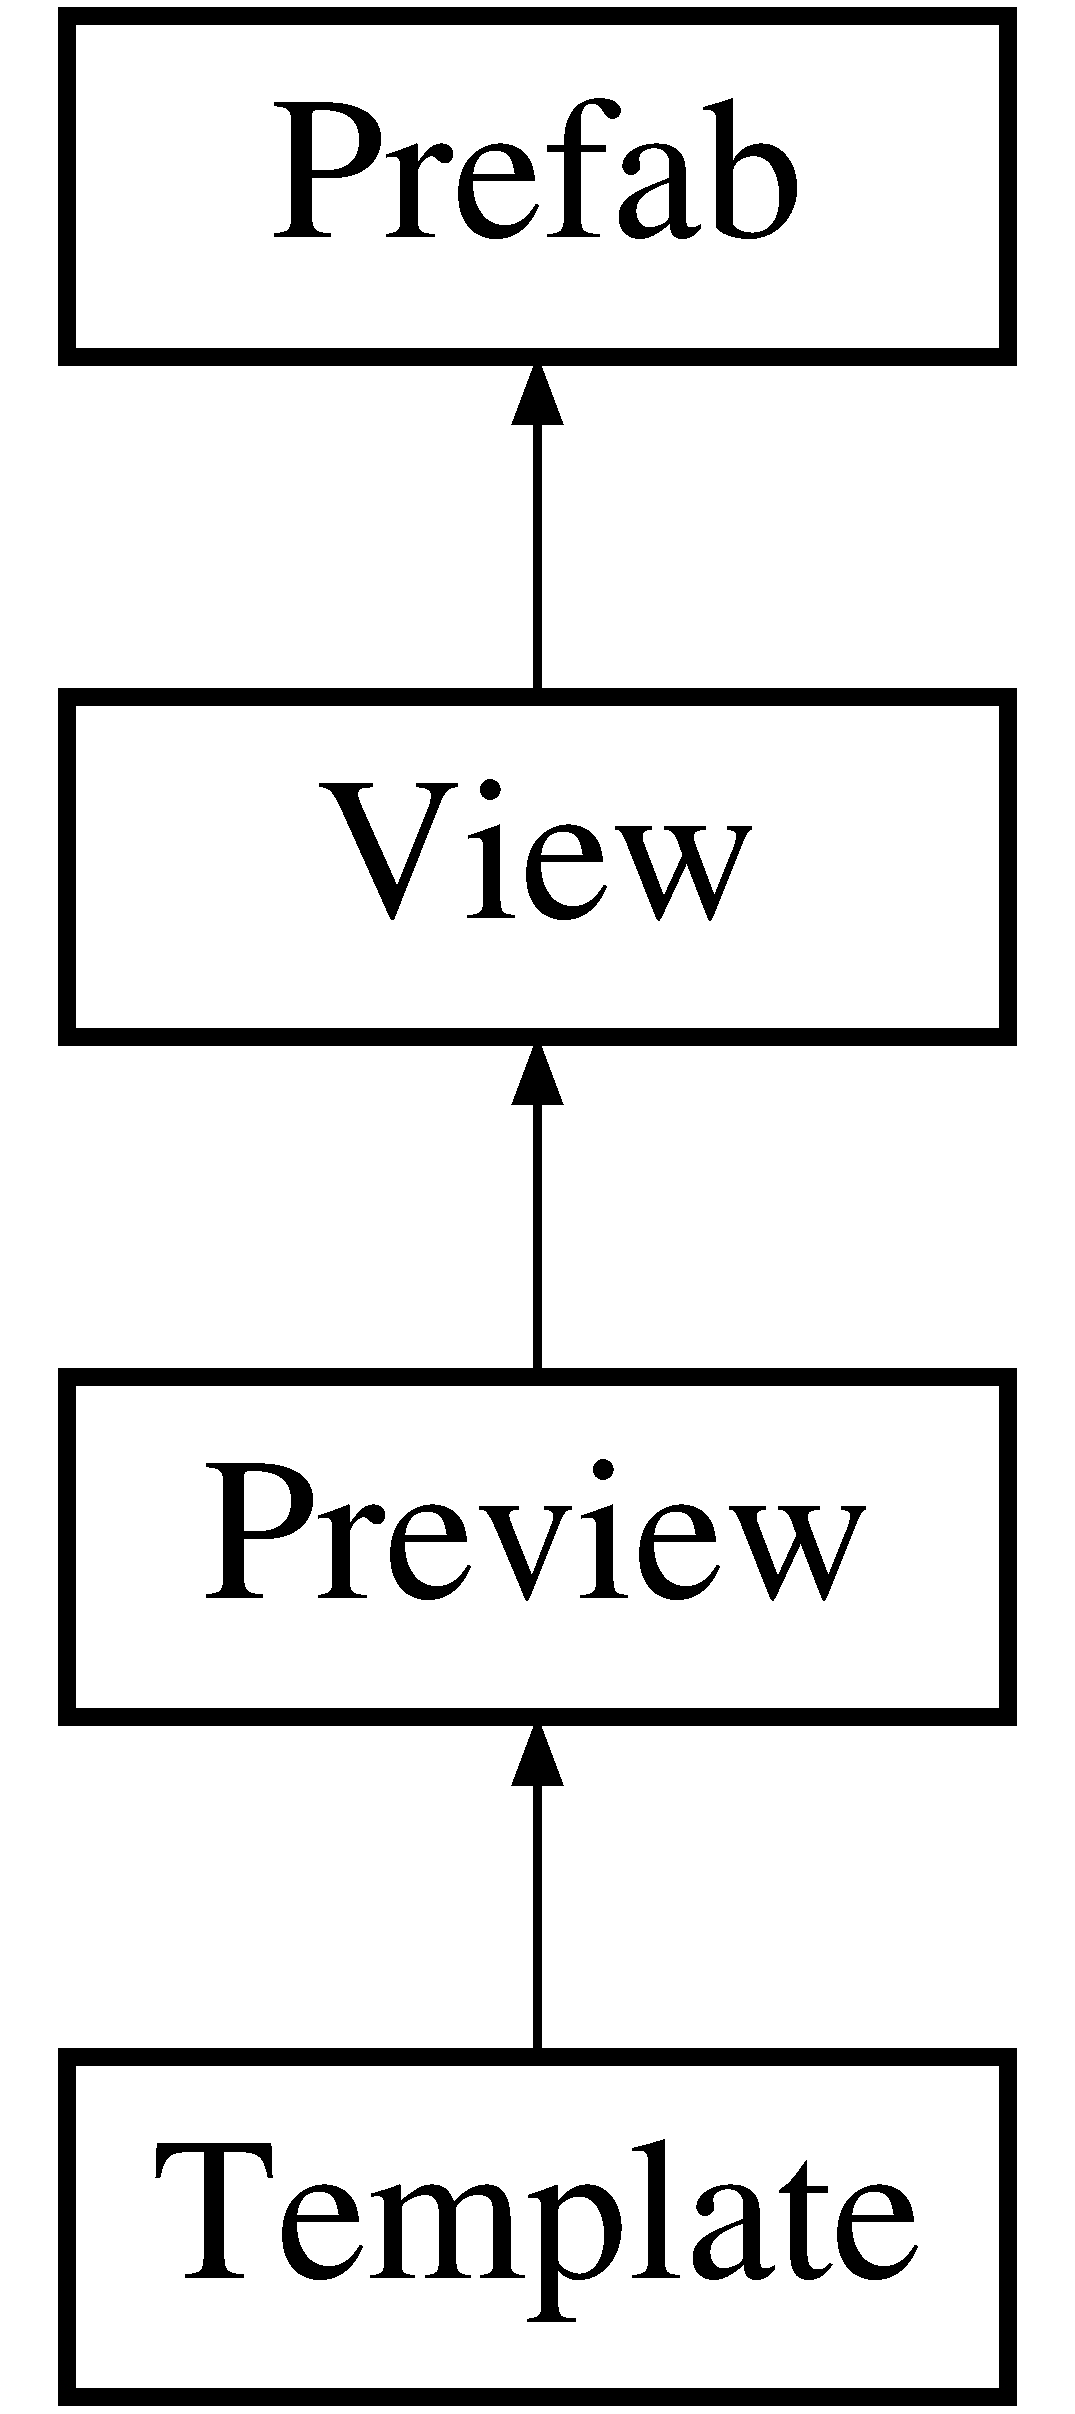
\includegraphics[height=4.000000cm]{class_preview}
\end{center}
\end{figure}
\subsection*{Public Member Functions}
\begin{DoxyCompactItemize}
\item 
\hyperlink{class_preview_a0a17b08b524058f3c3ce29d0985e83d6}{token} (\$str)
\item 
\hyperlink{class_preview_a739f9f012ec41e9b6ff99e88224f8c20}{filter} (\$key=N\+U\+LL, \$func=N\+U\+LL)
\item 
\hyperlink{class_preview_a2cc65dc50e9cabc431c6336705fd69eb}{resolve} (\$str, array \$hive=N\+U\+LL)
\item 
\hyperlink{class_preview_acddff385bc789c026a8530465c8c10ed}{render} (\$file, \$mime=N\+U\+LL, array \$hive=N\+U\+LL, \$ttl=0)
\end{DoxyCompactItemize}
\subsection*{Data Fields}
\begin{DoxyCompactItemize}
\item 
\hyperlink{class_preview_aac53bdb48bdd96ff9c20e2a86f48ce5f}{\$filter}
\begin{DoxyCompactList}\small\item\em token filter \end{DoxyCompactList}\end{DoxyCompactItemize}
\subsection*{Protected Member Functions}
\begin{DoxyCompactItemize}
\item 
\hyperlink{class_preview_a0e9d773ad8306b0d66337606414a443d}{build} (\$node)
\end{DoxyCompactItemize}
\subsection*{Protected Attributes}
\begin{DoxyCompactItemize}
\item 
\hypertarget{class_preview_a958cf7aca45cea5359ba0fa80ee2f2c1}{}\label{class_preview_a958cf7aca45cea5359ba0fa80ee2f2c1} 
\hyperlink{class_preview_a958cf7aca45cea5359ba0fa80ee2f2c1}{\$mime}
\begin{DoxyCompactList}\small\item\em M\+I\+ME type. \end{DoxyCompactList}\end{DoxyCompactItemize}
\subsection*{Additional Inherited Members}


\subsection{Detailed Description}
Lightweight template engine. 

Definition at line 2706 of file base.\+php.



\subsection{Member Function Documentation}
\hypertarget{class_preview_a0e9d773ad8306b0d66337606414a443d}{}\label{class_preview_a0e9d773ad8306b0d66337606414a443d} 
\index{Preview@{Preview}!build@{build}}
\index{build@{build}!Preview@{Preview}}
\subsubsection{\texorpdfstring{build()}{build()}}
{\footnotesize\ttfamily build (\begin{DoxyParamCaption}\item[{}]{\$node }\end{DoxyParamCaption})\hspace{0.3cm}{\ttfamily [protected]}}

Assemble markup \begin{DoxyReturn}{Returns}
string 
\end{DoxyReturn}

\begin{DoxyParams}{Parameters}
{\em \$node} & string \\
\hline
\end{DoxyParams}


Definition at line 2758 of file base.\+php.

\hypertarget{class_preview_a739f9f012ec41e9b6ff99e88224f8c20}{}\label{class_preview_a739f9f012ec41e9b6ff99e88224f8c20} 
\index{Preview@{Preview}!filter@{filter}}
\index{filter@{filter}!Preview@{Preview}}
\subsubsection{\texorpdfstring{filter()}{filter()}}
{\footnotesize\ttfamily filter (\begin{DoxyParamCaption}\item[{}]{\$key = {\ttfamily NULL},  }\item[{}]{\$func = {\ttfamily NULL} }\end{DoxyParamCaption})}

Register or get (a specific one or all) token filters 
\begin{DoxyParams}[1]{Parameters}
string & {\em \$key} & \\
\hline
string | closure & {\em \$func} & \\
\hline
\end{DoxyParams}
\begin{DoxyReturn}{Returns}
array$\vert$closure$\vert$string 
\end{DoxyReturn}


Definition at line 2745 of file base.\+php.

\hypertarget{class_preview_acddff385bc789c026a8530465c8c10ed}{}\label{class_preview_acddff385bc789c026a8530465c8c10ed} 
\index{Preview@{Preview}!render@{render}}
\index{render@{render}!Preview@{Preview}}
\subsubsection{\texorpdfstring{render()}{render()}}
{\footnotesize\ttfamily render (\begin{DoxyParamCaption}\item[{}]{\$file,  }\item[{}]{\$mime = {\ttfamily NULL},  }\item[{array}]{\$hive = {\ttfamily NULL},  }\item[{}]{\$ttl = {\ttfamily 0} }\end{DoxyParamCaption})}

Render template \begin{DoxyReturn}{Returns}
string 
\end{DoxyReturn}

\begin{DoxyParams}{Parameters}
{\em \$file} & string \\
\hline
{\em \$mime} & string \\
\hline
{\em \$hive} & array \\
\hline
{\em \$ttl} & int \\
\hline
\end{DoxyParams}


Definition at line 2804 of file base.\+php.

\hypertarget{class_preview_a2cc65dc50e9cabc431c6336705fd69eb}{}\label{class_preview_a2cc65dc50e9cabc431c6336705fd69eb} 
\index{Preview@{Preview}!resolve@{resolve}}
\index{resolve@{resolve}!Preview@{Preview}}
\subsubsection{\texorpdfstring{resolve()}{resolve()}}
{\footnotesize\ttfamily resolve (\begin{DoxyParamCaption}\item[{}]{\$str,  }\item[{array}]{\$hive = {\ttfamily NULL} }\end{DoxyParamCaption})}

Render template string \begin{DoxyReturn}{Returns}
string 
\end{DoxyReturn}

\begin{DoxyParams}{Parameters}
{\em \$str} & string \\
\hline
{\em \$hive} & array \\
\hline
\end{DoxyParams}


Definition at line 2787 of file base.\+php.

\hypertarget{class_preview_a0a17b08b524058f3c3ce29d0985e83d6}{}\label{class_preview_a0a17b08b524058f3c3ce29d0985e83d6} 
\index{Preview@{Preview}!token@{token}}
\index{token@{token}!Preview@{Preview}}
\subsubsection{\texorpdfstring{token()}{token()}}
{\footnotesize\ttfamily token (\begin{DoxyParamCaption}\item[{}]{\$str }\end{DoxyParamCaption})}

Convert token to variable \begin{DoxyReturn}{Returns}
string 
\end{DoxyReturn}

\begin{DoxyParams}{Parameters}
{\em \$str} & string \\
\hline
\end{DoxyParams}


Definition at line 2724 of file base.\+php.



\subsection{Field Documentation}
\hypertarget{class_preview_aac53bdb48bdd96ff9c20e2a86f48ce5f}{}\label{class_preview_aac53bdb48bdd96ff9c20e2a86f48ce5f} 
\index{Preview@{Preview}!\$filter@{\$filter}}
\index{\$filter@{\$filter}!Preview@{Preview}}
\subsubsection{\texorpdfstring{\$filter}{$filter}}
{\footnotesize\ttfamily \$\hyperlink{class_preview_a739f9f012ec41e9b6ff99e88224f8c20}{filter}}

{\bfseries Initial value\+:}
\begin{DoxyCode}
=[
            \textcolor{stringliteral}{'esc'}=>\textcolor{stringliteral}{'$this->esc'}
\end{DoxyCode}


token filter 



Definition at line 2712 of file base.\+php.



The documentation for this class was generated from the following file\+:\begin{DoxyCompactItemize}
\item 
/\+Users/aplennevaux/\+G\+I\+T\+H\+U\+B/\+Visionary-\/website/src/vendor/bcosca/fatfree/lib/base.\+php\end{DoxyCompactItemize}

\hypertarget{class_registry}{}\section{Registry Class Reference}
\label{class_registry}\index{Registry@{Registry}}


Container for singular object instances.  


\subsection*{Static Public Member Functions}
\begin{DoxyCompactItemize}
\item 
static \hyperlink{class_registry_a1a924eadddd0dc6fd3f6604a2352d950}{exists} (\$key)
\item 
static \hyperlink{class_registry_a8e135dfaf92afaa049c3f0bfe3437820}{set} (\$key, \$obj)
\item 
static \hyperlink{class_registry_a15e2679f2a8f6fa4d60757f4d65413ac}{get} (\$key)
\item 
static \hyperlink{class_registry_acc8237f9189f8ad2a9d854895561dbc2}{clear} (\$key)
\end{DoxyCompactItemize}


\subsection{Detailed Description}
Container for singular object instances. 

Definition at line 3212 of file base.\+php.



\subsection{Member Function Documentation}
\hypertarget{class_registry_acc8237f9189f8ad2a9d854895561dbc2}{}\label{class_registry_acc8237f9189f8ad2a9d854895561dbc2} 
\index{Registry@{Registry}!clear@{clear}}
\index{clear@{clear}!Registry@{Registry}}
\subsubsection{\texorpdfstring{clear()}{clear()}}
{\footnotesize\ttfamily static clear (\begin{DoxyParamCaption}\item[{}]{\$key }\end{DoxyParamCaption})\hspace{0.3cm}{\ttfamily [static]}}

Delete object from catalog \begin{DoxyReturn}{Returns}
N\+U\+LL 
\end{DoxyReturn}

\begin{DoxyParams}{Parameters}
{\em \$key} & string \\
\hline
\end{DoxyParams}


Definition at line 3251 of file base.\+php.

\hypertarget{class_registry_a1a924eadddd0dc6fd3f6604a2352d950}{}\label{class_registry_a1a924eadddd0dc6fd3f6604a2352d950} 
\index{Registry@{Registry}!exists@{exists}}
\index{exists@{exists}!Registry@{Registry}}
\subsubsection{\texorpdfstring{exists()}{exists()}}
{\footnotesize\ttfamily static exists (\begin{DoxyParamCaption}\item[{}]{\$key }\end{DoxyParamCaption})\hspace{0.3cm}{\ttfamily [static]}}

Return T\+R\+UE if object exists in catalog \begin{DoxyReturn}{Returns}
bool 
\end{DoxyReturn}

\begin{DoxyParams}{Parameters}
{\em \$key} & string \\
\hline
\end{DoxyParams}


Definition at line 3223 of file base.\+php.

\hypertarget{class_registry_a15e2679f2a8f6fa4d60757f4d65413ac}{}\label{class_registry_a15e2679f2a8f6fa4d60757f4d65413ac} 
\index{Registry@{Registry}!get@{get}}
\index{get@{get}!Registry@{Registry}}
\subsubsection{\texorpdfstring{get()}{get()}}
{\footnotesize\ttfamily static get (\begin{DoxyParamCaption}\item[{}]{\$key }\end{DoxyParamCaption})\hspace{0.3cm}{\ttfamily [static]}}

Retrieve object from catalog \begin{DoxyReturn}{Returns}
object 
\end{DoxyReturn}

\begin{DoxyParams}{Parameters}
{\em \$key} & string \\
\hline
\end{DoxyParams}


Definition at line 3242 of file base.\+php.

\hypertarget{class_registry_a8e135dfaf92afaa049c3f0bfe3437820}{}\label{class_registry_a8e135dfaf92afaa049c3f0bfe3437820} 
\index{Registry@{Registry}!set@{set}}
\index{set@{set}!Registry@{Registry}}
\subsubsection{\texorpdfstring{set()}{set()}}
{\footnotesize\ttfamily static set (\begin{DoxyParamCaption}\item[{}]{\$key,  }\item[{}]{\$obj }\end{DoxyParamCaption})\hspace{0.3cm}{\ttfamily [static]}}

Add object to catalog \begin{DoxyReturn}{Returns}
object 
\end{DoxyReturn}

\begin{DoxyParams}{Parameters}
{\em \$key} & string \\
\hline
{\em \$obj} & object \\
\hline
\end{DoxyParams}


Definition at line 3233 of file base.\+php.



The documentation for this class was generated from the following file\+:\begin{DoxyCompactItemize}
\item 
/\+Users/aplennevaux/\+G\+I\+T\+H\+U\+B/\+Visionary-\/website/src/vendor/bcosca/fatfree/lib/base.\+php\end{DoxyCompactItemize}

\hypertarget{class_d_b_1_1_mongo_1_1_session}{}\section{Session Class Reference}
\label{class_d_b_1_1_mongo_1_1_session}\index{Session@{Session}}


Mongo\+D\+B-\/managed session handler.  


Inheritance diagram for Session\+:\begin{figure}[H]
\begin{center}
\leavevmode
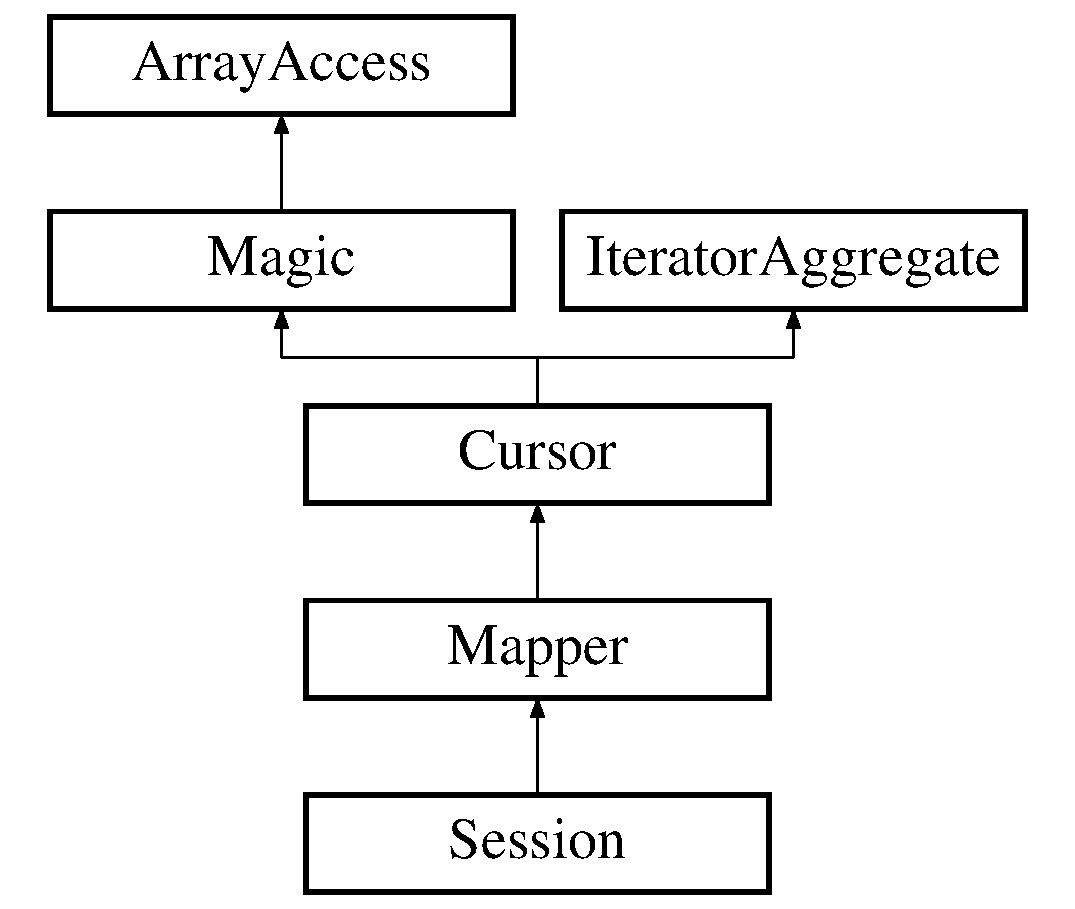
\includegraphics[height=5.000000cm]{class_d_b_1_1_mongo_1_1_session}
\end{center}
\end{figure}
\subsection*{Public Member Functions}
\begin{DoxyCompactItemize}
\item 
\hyperlink{class_d_b_1_1_mongo_1_1_session_a037c59224bcb347b69ca61df88ef7230}{open} (\$path, \$name)
\item 
\hyperlink{class_d_b_1_1_mongo_1_1_session_aa69c8bf1f1dcf4e72552efff1fe3e87e}{close} ()
\item 
\hyperlink{class_d_b_1_1_mongo_1_1_session_afa59bebedda70c37b94c2efc35da83f3}{read} (\$id)
\item 
\hyperlink{class_d_b_1_1_mongo_1_1_session_a5f277b5f0e4e2154cddc9a3a0d2bf57d}{write} (\$id, \$data)
\item 
\hyperlink{class_d_b_1_1_mongo_1_1_session_a726fa8a4b4b187b9ca32ba427aac8137}{destroy} (\$id)
\item 
\hyperlink{class_d_b_1_1_mongo_1_1_session_a60b027eb0df6d42b8fe2ec8c93cfbbae}{cleanup} (\$max)
\item 
\hyperlink{class_d_b_1_1_mongo_1_1_session_a30b416c35150ab6bdde364f527f612bd}{sid} ()
\item 
\hyperlink{class_d_b_1_1_mongo_1_1_session_a048d24aa22a28f92f1f3a7e3d323f45e}{csrf} ()
\item 
\hyperlink{class_d_b_1_1_mongo_1_1_session_a197bae3714812901860bd006b00f91de}{ip} ()
\item 
\hyperlink{class_d_b_1_1_mongo_1_1_session_ab0b8b94527259f4aacdf1fd45411abfe}{stamp} ()
\item 
\hyperlink{class_d_b_1_1_mongo_1_1_session_a77f6a261d70e66c7b7273774832482dc}{agent} ()
\item 
\hyperlink{class_d_b_1_1_mongo_1_1_session_ada564f6a7ed0e500e4dcb57e02e03c83}{\+\_\+\+\_\+construct} (\textbackslash{}\hyperlink{class_d_b_1_1_mongo}{D\+B\textbackslash{}\+Mongo} \$db, \$table=\textquotesingle{}sessions\textquotesingle{}, \$onsuspect=N\+U\+LL, \$key=N\+U\+LL)
\end{DoxyCompactItemize}
\subsection*{Data Fields}
\begin{DoxyCompactItemize}
\item 
\hypertarget{class_d_b_1_1_mongo_1_1_session_a871411a78a77c508569c380dd06fdd51}{}\label{class_d_b_1_1_mongo_1_1_session_a871411a78a77c508569c380dd06fdd51} 
\hyperlink{class_d_b_1_1_mongo_1_1_session_a871411a78a77c508569c380dd06fdd51}{\$\+\_\+csrf}
\begin{DoxyCompactList}\small\item\em Anti-\/\+C\+S\+RF token. \end{DoxyCompactList}\item 
\hypertarget{class_d_b_1_1_mongo_1_1_session_a7e43e09863a494197e0cdbf3f98c2ff5}{}\label{class_d_b_1_1_mongo_1_1_session_a7e43e09863a494197e0cdbf3f98c2ff5} 
\hyperlink{class_d_b_1_1_mongo_1_1_session_a7e43e09863a494197e0cdbf3f98c2ff5}{\$\+\_\+agent}
\begin{DoxyCompactList}\small\item\em User agent. \end{DoxyCompactList}\item 
\hypertarget{class_d_b_1_1_mongo_1_1_session_ac275a475a83ee8de16cf9c9f928fbe77}{}\label{class_d_b_1_1_mongo_1_1_session_ac275a475a83ee8de16cf9c9f928fbe77} 
\hyperlink{class_d_b_1_1_mongo_1_1_session_ac275a475a83ee8de16cf9c9f928fbe77}{\$\+\_\+ip}
\begin{DoxyCompactList}\small\item\em IP,. \end{DoxyCompactList}\item 
\hypertarget{class_d_b_1_1_mongo_1_1_session_ad96efa4953d3355e4c1aabc5cebad482}{}\label{class_d_b_1_1_mongo_1_1_session_ad96efa4953d3355e4c1aabc5cebad482} 
\hyperlink{class_d_b_1_1_mongo_1_1_session_ad96efa4953d3355e4c1aabc5cebad482}{\$onsuspect}
\begin{DoxyCompactList}\small\item\em Suspect callback. \end{DoxyCompactList}\end{DoxyCompactItemize}
\subsection*{Protected Attributes}
\begin{DoxyCompactItemize}
\item 
\hypertarget{class_d_b_1_1_mongo_1_1_session_a3b4e4b29ac1d6699dd65f8f0d6fa4133}{}\label{class_d_b_1_1_mongo_1_1_session_a3b4e4b29ac1d6699dd65f8f0d6fa4133} 
\hyperlink{class_d_b_1_1_mongo_1_1_session_a3b4e4b29ac1d6699dd65f8f0d6fa4133}{\$sid}
\begin{DoxyCompactList}\small\item\em \hyperlink{class_d_b_1_1_mongo_1_1_session}{Session} ID. \end{DoxyCompactList}\end{DoxyCompactItemize}
\subsection*{Additional Inherited Members}


\subsection{Detailed Description}
Mongo\+D\+B-\/managed session handler. 

Definition at line 26 of file session.\+php.



\subsection{Constructor \& Destructor Documentation}
\hypertarget{class_d_b_1_1_mongo_1_1_session_ada564f6a7ed0e500e4dcb57e02e03c83}{}\label{class_d_b_1_1_mongo_1_1_session_ada564f6a7ed0e500e4dcb57e02e03c83} 
\index{D\+B\+::\+Mongo\+::\+Session@{D\+B\+::\+Mongo\+::\+Session}!\+\_\+\+\_\+construct@{\+\_\+\+\_\+construct}}
\index{\+\_\+\+\_\+construct@{\+\_\+\+\_\+construct}!D\+B\+::\+Mongo\+::\+Session@{D\+B\+::\+Mongo\+::\+Session}}
\subsubsection{\texorpdfstring{\+\_\+\+\_\+construct()}{\_\_construct()}}
{\footnotesize\ttfamily \+\_\+\+\_\+construct (\begin{DoxyParamCaption}\item[{\textbackslash{}\hyperlink{class_d_b_1_1_mongo}{D\+B\textbackslash{}\+Mongo}}]{\$db,  }\item[{}]{\$table = {\ttfamily \textquotesingle{}sessions\textquotesingle{}},  }\item[{}]{\$onsuspect = {\ttfamily NULL},  }\item[{}]{\$key = {\ttfamily NULL} }\end{DoxyParamCaption})}

Instantiate class 
\begin{DoxyParams}{Parameters}
{\em \$db} & \\
\hline
{\em \$table} & string \\
\hline
{\em \$onsuspect} & callback \\
\hline
{\em \$key} & string \\
\hline
\end{DoxyParams}


Definition at line 168 of file session.\+php.



\subsection{Member Function Documentation}
\hypertarget{class_d_b_1_1_mongo_1_1_session_a77f6a261d70e66c7b7273774832482dc}{}\label{class_d_b_1_1_mongo_1_1_session_a77f6a261d70e66c7b7273774832482dc} 
\index{D\+B\+::\+Mongo\+::\+Session@{D\+B\+::\+Mongo\+::\+Session}!agent@{agent}}
\index{agent@{agent}!D\+B\+::\+Mongo\+::\+Session@{D\+B\+::\+Mongo\+::\+Session}}
\subsubsection{\texorpdfstring{agent()}{agent()}}
{\footnotesize\ttfamily agent (\begin{DoxyParamCaption}{ }\end{DoxyParamCaption})}

Return H\+T\+TP user agent \begin{DoxyReturn}{Returns}
string 
\end{DoxyReturn}


Definition at line 157 of file session.\+php.

\hypertarget{class_d_b_1_1_mongo_1_1_session_a60b027eb0df6d42b8fe2ec8c93cfbbae}{}\label{class_d_b_1_1_mongo_1_1_session_a60b027eb0df6d42b8fe2ec8c93cfbbae} 
\index{D\+B\+::\+Mongo\+::\+Session@{D\+B\+::\+Mongo\+::\+Session}!cleanup@{cleanup}}
\index{cleanup@{cleanup}!D\+B\+::\+Mongo\+::\+Session@{D\+B\+::\+Mongo\+::\+Session}}
\subsubsection{\texorpdfstring{cleanup()}{cleanup()}}
{\footnotesize\ttfamily cleanup (\begin{DoxyParamCaption}\item[{}]{\$max }\end{DoxyParamCaption})}

Garbage collector \begin{DoxyReturn}{Returns}
T\+R\+UE 
\end{DoxyReturn}

\begin{DoxyParams}{Parameters}
{\em \$max} & int \\
\hline
\end{DoxyParams}


Definition at line 114 of file session.\+php.

\hypertarget{class_d_b_1_1_mongo_1_1_session_aa69c8bf1f1dcf4e72552efff1fe3e87e}{}\label{class_d_b_1_1_mongo_1_1_session_aa69c8bf1f1dcf4e72552efff1fe3e87e} 
\index{D\+B\+::\+Mongo\+::\+Session@{D\+B\+::\+Mongo\+::\+Session}!close@{close}}
\index{close@{close}!D\+B\+::\+Mongo\+::\+Session@{D\+B\+::\+Mongo\+::\+Session}}
\subsubsection{\texorpdfstring{close()}{close()}}
{\footnotesize\ttfamily close (\begin{DoxyParamCaption}{ }\end{DoxyParamCaption})}

Close session \begin{DoxyReturn}{Returns}
T\+R\+UE 
\end{DoxyReturn}


Definition at line 54 of file session.\+php.

\hypertarget{class_d_b_1_1_mongo_1_1_session_a048d24aa22a28f92f1f3a7e3d323f45e}{}\label{class_d_b_1_1_mongo_1_1_session_a048d24aa22a28f92f1f3a7e3d323f45e} 
\index{D\+B\+::\+Mongo\+::\+Session@{D\+B\+::\+Mongo\+::\+Session}!csrf@{csrf}}
\index{csrf@{csrf}!D\+B\+::\+Mongo\+::\+Session@{D\+B\+::\+Mongo\+::\+Session}}
\subsubsection{\texorpdfstring{csrf()}{csrf()}}
{\footnotesize\ttfamily csrf (\begin{DoxyParamCaption}{ }\end{DoxyParamCaption})}

Return anti-\/\+C\+S\+RF token \begin{DoxyReturn}{Returns}
string 
\end{DoxyReturn}


Definition at line 131 of file session.\+php.

\hypertarget{class_d_b_1_1_mongo_1_1_session_a726fa8a4b4b187b9ca32ba427aac8137}{}\label{class_d_b_1_1_mongo_1_1_session_a726fa8a4b4b187b9ca32ba427aac8137} 
\index{D\+B\+::\+Mongo\+::\+Session@{D\+B\+::\+Mongo\+::\+Session}!destroy@{destroy}}
\index{destroy@{destroy}!D\+B\+::\+Mongo\+::\+Session@{D\+B\+::\+Mongo\+::\+Session}}
\subsubsection{\texorpdfstring{destroy()}{destroy()}}
{\footnotesize\ttfamily destroy (\begin{DoxyParamCaption}\item[{}]{\$id }\end{DoxyParamCaption})}

Destroy session \begin{DoxyReturn}{Returns}
T\+R\+UE 
\end{DoxyReturn}

\begin{DoxyParams}{Parameters}
{\em \$id} & string \\
\hline
\end{DoxyParams}


Definition at line 104 of file session.\+php.

\hypertarget{class_d_b_1_1_mongo_1_1_session_a197bae3714812901860bd006b00f91de}{}\label{class_d_b_1_1_mongo_1_1_session_a197bae3714812901860bd006b00f91de} 
\index{D\+B\+::\+Mongo\+::\+Session@{D\+B\+::\+Mongo\+::\+Session}!ip@{ip}}
\index{ip@{ip}!D\+B\+::\+Mongo\+::\+Session@{D\+B\+::\+Mongo\+::\+Session}}
\subsubsection{\texorpdfstring{ip()}{ip()}}
{\footnotesize\ttfamily ip (\begin{DoxyParamCaption}{ }\end{DoxyParamCaption})}

Return IP address \begin{DoxyReturn}{Returns}
string 
\end{DoxyReturn}


Definition at line 139 of file session.\+php.

\hypertarget{class_d_b_1_1_mongo_1_1_session_a037c59224bcb347b69ca61df88ef7230}{}\label{class_d_b_1_1_mongo_1_1_session_a037c59224bcb347b69ca61df88ef7230} 
\index{D\+B\+::\+Mongo\+::\+Session@{D\+B\+::\+Mongo\+::\+Session}!open@{open}}
\index{open@{open}!D\+B\+::\+Mongo\+::\+Session@{D\+B\+::\+Mongo\+::\+Session}}
\subsubsection{\texorpdfstring{open()}{open()}}
{\footnotesize\ttfamily open (\begin{DoxyParamCaption}\item[{}]{\$path,  }\item[{}]{\$name }\end{DoxyParamCaption})}

Open session \begin{DoxyReturn}{Returns}
T\+R\+UE 
\end{DoxyReturn}

\begin{DoxyParams}{Parameters}
{\em \$path} & string \\
\hline
{\em \$name} & string \\
\hline
\end{DoxyParams}


Definition at line 46 of file session.\+php.

\hypertarget{class_d_b_1_1_mongo_1_1_session_afa59bebedda70c37b94c2efc35da83f3}{}\label{class_d_b_1_1_mongo_1_1_session_afa59bebedda70c37b94c2efc35da83f3} 
\index{D\+B\+::\+Mongo\+::\+Session@{D\+B\+::\+Mongo\+::\+Session}!read@{read}}
\index{read@{read}!D\+B\+::\+Mongo\+::\+Session@{D\+B\+::\+Mongo\+::\+Session}}
\subsubsection{\texorpdfstring{read()}{read()}}
{\footnotesize\ttfamily read (\begin{DoxyParamCaption}\item[{}]{\$id }\end{DoxyParamCaption})}

Return session data in serialized format \begin{DoxyReturn}{Returns}
string$\vert$\+F\+A\+L\+SE 
\end{DoxyReturn}

\begin{DoxyParams}{Parameters}
{\em \$id} & string \\
\hline
\end{DoxyParams}


Definition at line 65 of file session.\+php.

\hypertarget{class_d_b_1_1_mongo_1_1_session_a30b416c35150ab6bdde364f527f612bd}{}\label{class_d_b_1_1_mongo_1_1_session_a30b416c35150ab6bdde364f527f612bd} 
\index{D\+B\+::\+Mongo\+::\+Session@{D\+B\+::\+Mongo\+::\+Session}!sid@{sid}}
\index{sid@{sid}!D\+B\+::\+Mongo\+::\+Session@{D\+B\+::\+Mongo\+::\+Session}}
\subsubsection{\texorpdfstring{sid()}{sid()}}
{\footnotesize\ttfamily sid (\begin{DoxyParamCaption}{ }\end{DoxyParamCaption})}

Return session id (if session has started) \begin{DoxyReturn}{Returns}
string$\vert$\+N\+U\+LL 
\end{DoxyReturn}


Definition at line 123 of file session.\+php.

\hypertarget{class_d_b_1_1_mongo_1_1_session_ab0b8b94527259f4aacdf1fd45411abfe}{}\label{class_d_b_1_1_mongo_1_1_session_ab0b8b94527259f4aacdf1fd45411abfe} 
\index{D\+B\+::\+Mongo\+::\+Session@{D\+B\+::\+Mongo\+::\+Session}!stamp@{stamp}}
\index{stamp@{stamp}!D\+B\+::\+Mongo\+::\+Session@{D\+B\+::\+Mongo\+::\+Session}}
\subsubsection{\texorpdfstring{stamp()}{stamp()}}
{\footnotesize\ttfamily stamp (\begin{DoxyParamCaption}{ }\end{DoxyParamCaption})}

Return Unix timestamp \begin{DoxyReturn}{Returns}
string$\vert$\+F\+A\+L\+SE 
\end{DoxyReturn}


Definition at line 147 of file session.\+php.

\hypertarget{class_d_b_1_1_mongo_1_1_session_a5f277b5f0e4e2154cddc9a3a0d2bf57d}{}\label{class_d_b_1_1_mongo_1_1_session_a5f277b5f0e4e2154cddc9a3a0d2bf57d} 
\index{D\+B\+::\+Mongo\+::\+Session@{D\+B\+::\+Mongo\+::\+Session}!write@{write}}
\index{write@{write}!D\+B\+::\+Mongo\+::\+Session@{D\+B\+::\+Mongo\+::\+Session}}
\subsubsection{\texorpdfstring{write()}{write()}}
{\footnotesize\ttfamily write (\begin{DoxyParamCaption}\item[{}]{\$id,  }\item[{}]{\$data }\end{DoxyParamCaption})}

Write session data \begin{DoxyReturn}{Returns}
T\+R\+UE 
\end{DoxyReturn}

\begin{DoxyParams}{Parameters}
{\em \$id} & string \\
\hline
{\em \$data} & string \\
\hline
\end{DoxyParams}


Definition at line 89 of file session.\+php.



The documentation for this class was generated from the following file\+:\begin{DoxyCompactItemize}
\item 
/\+Users/aplennevaux/\+G\+I\+T\+H\+U\+B/\+Visionary-\/website/src/vendor/bcosca/fatfree/lib/db/mongo/session.\+php\end{DoxyCompactItemize}

\hypertarget{class_d_b_1_1_jig_1_1_session}{}\section{Session Class Reference}
\label{class_d_b_1_1_jig_1_1_session}\index{Session@{Session}}


Jig-\/managed session handler.  


Inheritance diagram for Session\+:\begin{figure}[H]
\begin{center}
\leavevmode
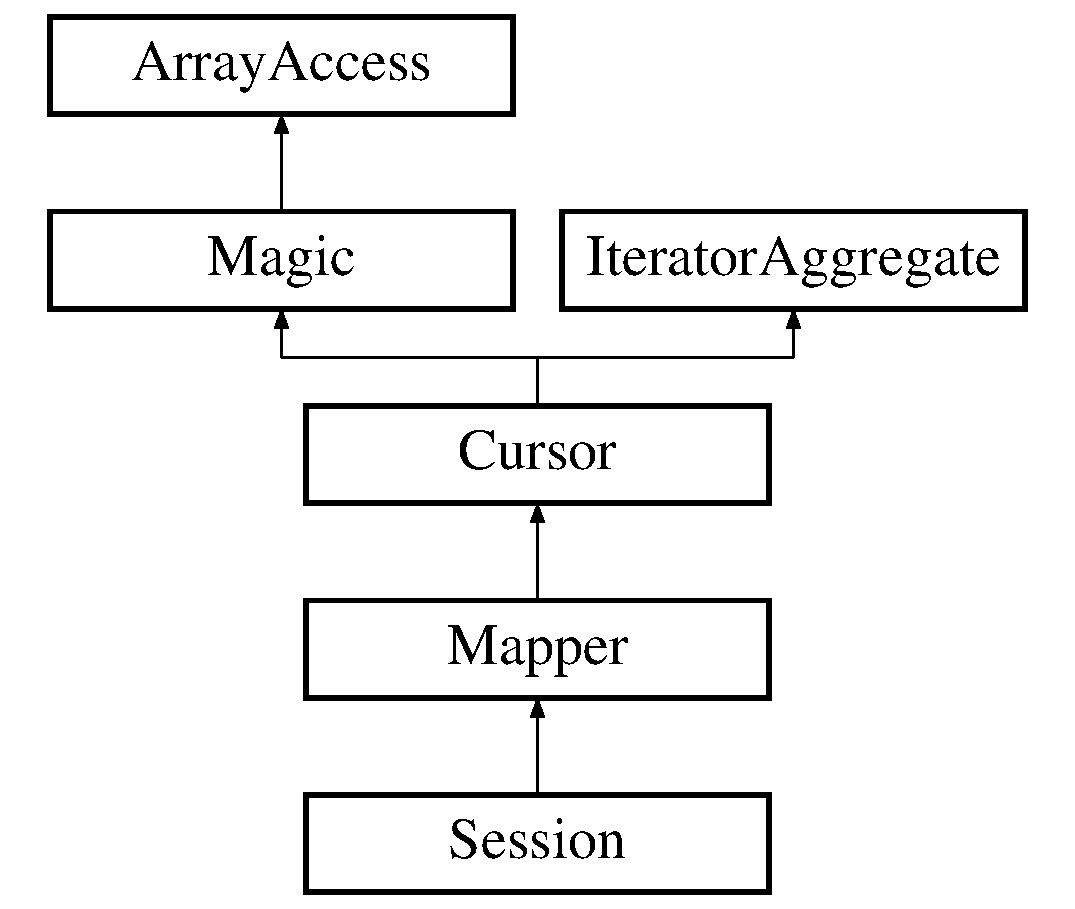
\includegraphics[height=5.000000cm]{class_d_b_1_1_jig_1_1_session}
\end{center}
\end{figure}
\subsection*{Public Member Functions}
\begin{DoxyCompactItemize}
\item 
\hyperlink{class_d_b_1_1_jig_1_1_session_a037c59224bcb347b69ca61df88ef7230}{open} (\$path, \$name)
\item 
\hyperlink{class_d_b_1_1_jig_1_1_session_aa69c8bf1f1dcf4e72552efff1fe3e87e}{close} ()
\item 
\hyperlink{class_d_b_1_1_jig_1_1_session_afa59bebedda70c37b94c2efc35da83f3}{read} (\$id)
\item 
\hyperlink{class_d_b_1_1_jig_1_1_session_a5f277b5f0e4e2154cddc9a3a0d2bf57d}{write} (\$id, \$data)
\item 
\hyperlink{class_d_b_1_1_jig_1_1_session_a726fa8a4b4b187b9ca32ba427aac8137}{destroy} (\$id)
\item 
\hyperlink{class_d_b_1_1_jig_1_1_session_a60b027eb0df6d42b8fe2ec8c93cfbbae}{cleanup} (\$max)
\item 
\hyperlink{class_d_b_1_1_jig_1_1_session_a30b416c35150ab6bdde364f527f612bd}{sid} ()
\item 
\hyperlink{class_d_b_1_1_jig_1_1_session_a048d24aa22a28f92f1f3a7e3d323f45e}{csrf} ()
\item 
\hyperlink{class_d_b_1_1_jig_1_1_session_a197bae3714812901860bd006b00f91de}{ip} ()
\item 
\hyperlink{class_d_b_1_1_jig_1_1_session_ab0b8b94527259f4aacdf1fd45411abfe}{stamp} ()
\item 
\hyperlink{class_d_b_1_1_jig_1_1_session_a77f6a261d70e66c7b7273774832482dc}{agent} ()
\item 
\hyperlink{class_d_b_1_1_jig_1_1_session_a7e7d0206d7feb1eb2ff8b121078243bd}{\+\_\+\+\_\+construct} (\textbackslash{}\hyperlink{class_d_b_1_1_jig}{D\+B\textbackslash{}\+Jig} \$db, \$file=\textquotesingle{}sessions\textquotesingle{}, \$onsuspect=N\+U\+LL, \$key=N\+U\+LL)
\end{DoxyCompactItemize}
\subsection*{Data Fields}
\begin{DoxyCompactItemize}
\item 
\hypertarget{class_d_b_1_1_jig_1_1_session_a871411a78a77c508569c380dd06fdd51}{}\label{class_d_b_1_1_jig_1_1_session_a871411a78a77c508569c380dd06fdd51} 
\hyperlink{class_d_b_1_1_jig_1_1_session_a871411a78a77c508569c380dd06fdd51}{\$\+\_\+csrf}
\begin{DoxyCompactList}\small\item\em Anti-\/\+C\+S\+RF token. \end{DoxyCompactList}\item 
\hypertarget{class_d_b_1_1_jig_1_1_session_a7e43e09863a494197e0cdbf3f98c2ff5}{}\label{class_d_b_1_1_jig_1_1_session_a7e43e09863a494197e0cdbf3f98c2ff5} 
\hyperlink{class_d_b_1_1_jig_1_1_session_a7e43e09863a494197e0cdbf3f98c2ff5}{\$\+\_\+agent}
\begin{DoxyCompactList}\small\item\em User agent. \end{DoxyCompactList}\item 
\hypertarget{class_d_b_1_1_jig_1_1_session_ac275a475a83ee8de16cf9c9f928fbe77}{}\label{class_d_b_1_1_jig_1_1_session_ac275a475a83ee8de16cf9c9f928fbe77} 
\hyperlink{class_d_b_1_1_jig_1_1_session_ac275a475a83ee8de16cf9c9f928fbe77}{\$\+\_\+ip}
\begin{DoxyCompactList}\small\item\em IP,. \end{DoxyCompactList}\item 
\hypertarget{class_d_b_1_1_jig_1_1_session_ad96efa4953d3355e4c1aabc5cebad482}{}\label{class_d_b_1_1_jig_1_1_session_ad96efa4953d3355e4c1aabc5cebad482} 
\hyperlink{class_d_b_1_1_jig_1_1_session_ad96efa4953d3355e4c1aabc5cebad482}{\$onsuspect}
\begin{DoxyCompactList}\small\item\em Suspect callback. \end{DoxyCompactList}\end{DoxyCompactItemize}
\subsection*{Protected Attributes}
\begin{DoxyCompactItemize}
\item 
\hypertarget{class_d_b_1_1_jig_1_1_session_a3b4e4b29ac1d6699dd65f8f0d6fa4133}{}\label{class_d_b_1_1_jig_1_1_session_a3b4e4b29ac1d6699dd65f8f0d6fa4133} 
\hyperlink{class_d_b_1_1_jig_1_1_session_a3b4e4b29ac1d6699dd65f8f0d6fa4133}{\$sid}
\begin{DoxyCompactList}\small\item\em \hyperlink{class_d_b_1_1_jig_1_1_session}{Session} ID. \end{DoxyCompactList}\end{DoxyCompactItemize}
\subsection*{Additional Inherited Members}


\subsection{Detailed Description}
Jig-\/managed session handler. 

Definition at line 26 of file session.\+php.



\subsection{Constructor \& Destructor Documentation}
\hypertarget{class_d_b_1_1_jig_1_1_session_a7e7d0206d7feb1eb2ff8b121078243bd}{}\label{class_d_b_1_1_jig_1_1_session_a7e7d0206d7feb1eb2ff8b121078243bd} 
\index{D\+B\+::\+Jig\+::\+Session@{D\+B\+::\+Jig\+::\+Session}!\+\_\+\+\_\+construct@{\+\_\+\+\_\+construct}}
\index{\+\_\+\+\_\+construct@{\+\_\+\+\_\+construct}!D\+B\+::\+Jig\+::\+Session@{D\+B\+::\+Jig\+::\+Session}}
\subsubsection{\texorpdfstring{\+\_\+\+\_\+construct()}{\_\_construct()}}
{\footnotesize\ttfamily \+\_\+\+\_\+construct (\begin{DoxyParamCaption}\item[{\textbackslash{}\hyperlink{class_d_b_1_1_jig}{D\+B\textbackslash{}\+Jig}}]{\$db,  }\item[{}]{\$file = {\ttfamily \textquotesingle{}sessions\textquotesingle{}},  }\item[{}]{\$onsuspect = {\ttfamily NULL},  }\item[{}]{\$key = {\ttfamily NULL} }\end{DoxyParamCaption})}

Instantiate class 
\begin{DoxyParams}{Parameters}
{\em \$db} & \\
\hline
{\em \$file} & string \\
\hline
{\em \$onsuspect} & callback \\
\hline
{\em \$key} & string \\
\hline
\end{DoxyParams}


Definition at line 168 of file session.\+php.



\subsection{Member Function Documentation}
\hypertarget{class_d_b_1_1_jig_1_1_session_a77f6a261d70e66c7b7273774832482dc}{}\label{class_d_b_1_1_jig_1_1_session_a77f6a261d70e66c7b7273774832482dc} 
\index{D\+B\+::\+Jig\+::\+Session@{D\+B\+::\+Jig\+::\+Session}!agent@{agent}}
\index{agent@{agent}!D\+B\+::\+Jig\+::\+Session@{D\+B\+::\+Jig\+::\+Session}}
\subsubsection{\texorpdfstring{agent()}{agent()}}
{\footnotesize\ttfamily agent (\begin{DoxyParamCaption}{ }\end{DoxyParamCaption})}

Return H\+T\+TP user agent \begin{DoxyReturn}{Returns}
string$\vert$\+F\+A\+L\+SE 
\end{DoxyReturn}


Definition at line 157 of file session.\+php.

\hypertarget{class_d_b_1_1_jig_1_1_session_a60b027eb0df6d42b8fe2ec8c93cfbbae}{}\label{class_d_b_1_1_jig_1_1_session_a60b027eb0df6d42b8fe2ec8c93cfbbae} 
\index{D\+B\+::\+Jig\+::\+Session@{D\+B\+::\+Jig\+::\+Session}!cleanup@{cleanup}}
\index{cleanup@{cleanup}!D\+B\+::\+Jig\+::\+Session@{D\+B\+::\+Jig\+::\+Session}}
\subsubsection{\texorpdfstring{cleanup()}{cleanup()}}
{\footnotesize\ttfamily cleanup (\begin{DoxyParamCaption}\item[{}]{\$max }\end{DoxyParamCaption})}

Garbage collector \begin{DoxyReturn}{Returns}
T\+R\+UE 
\end{DoxyReturn}

\begin{DoxyParams}{Parameters}
{\em \$max} & int \\
\hline
\end{DoxyParams}


Definition at line 114 of file session.\+php.

\hypertarget{class_d_b_1_1_jig_1_1_session_aa69c8bf1f1dcf4e72552efff1fe3e87e}{}\label{class_d_b_1_1_jig_1_1_session_aa69c8bf1f1dcf4e72552efff1fe3e87e} 
\index{D\+B\+::\+Jig\+::\+Session@{D\+B\+::\+Jig\+::\+Session}!close@{close}}
\index{close@{close}!D\+B\+::\+Jig\+::\+Session@{D\+B\+::\+Jig\+::\+Session}}
\subsubsection{\texorpdfstring{close()}{close()}}
{\footnotesize\ttfamily close (\begin{DoxyParamCaption}{ }\end{DoxyParamCaption})}

Close session \begin{DoxyReturn}{Returns}
T\+R\+UE 
\end{DoxyReturn}


Definition at line 54 of file session.\+php.

\hypertarget{class_d_b_1_1_jig_1_1_session_a048d24aa22a28f92f1f3a7e3d323f45e}{}\label{class_d_b_1_1_jig_1_1_session_a048d24aa22a28f92f1f3a7e3d323f45e} 
\index{D\+B\+::\+Jig\+::\+Session@{D\+B\+::\+Jig\+::\+Session}!csrf@{csrf}}
\index{csrf@{csrf}!D\+B\+::\+Jig\+::\+Session@{D\+B\+::\+Jig\+::\+Session}}
\subsubsection{\texorpdfstring{csrf()}{csrf()}}
{\footnotesize\ttfamily csrf (\begin{DoxyParamCaption}{ }\end{DoxyParamCaption})}

Return anti-\/\+C\+S\+RF token \begin{DoxyReturn}{Returns}
string 
\end{DoxyReturn}


Definition at line 131 of file session.\+php.

\hypertarget{class_d_b_1_1_jig_1_1_session_a726fa8a4b4b187b9ca32ba427aac8137}{}\label{class_d_b_1_1_jig_1_1_session_a726fa8a4b4b187b9ca32ba427aac8137} 
\index{D\+B\+::\+Jig\+::\+Session@{D\+B\+::\+Jig\+::\+Session}!destroy@{destroy}}
\index{destroy@{destroy}!D\+B\+::\+Jig\+::\+Session@{D\+B\+::\+Jig\+::\+Session}}
\subsubsection{\texorpdfstring{destroy()}{destroy()}}
{\footnotesize\ttfamily destroy (\begin{DoxyParamCaption}\item[{}]{\$id }\end{DoxyParamCaption})}

Destroy session \begin{DoxyReturn}{Returns}
T\+R\+UE 
\end{DoxyReturn}

\begin{DoxyParams}{Parameters}
{\em \$id} & string \\
\hline
\end{DoxyParams}


Definition at line 104 of file session.\+php.

\hypertarget{class_d_b_1_1_jig_1_1_session_a197bae3714812901860bd006b00f91de}{}\label{class_d_b_1_1_jig_1_1_session_a197bae3714812901860bd006b00f91de} 
\index{D\+B\+::\+Jig\+::\+Session@{D\+B\+::\+Jig\+::\+Session}!ip@{ip}}
\index{ip@{ip}!D\+B\+::\+Jig\+::\+Session@{D\+B\+::\+Jig\+::\+Session}}
\subsubsection{\texorpdfstring{ip()}{ip()}}
{\footnotesize\ttfamily ip (\begin{DoxyParamCaption}{ }\end{DoxyParamCaption})}

Return IP address \begin{DoxyReturn}{Returns}
string 
\end{DoxyReturn}


Definition at line 139 of file session.\+php.

\hypertarget{class_d_b_1_1_jig_1_1_session_a037c59224bcb347b69ca61df88ef7230}{}\label{class_d_b_1_1_jig_1_1_session_a037c59224bcb347b69ca61df88ef7230} 
\index{D\+B\+::\+Jig\+::\+Session@{D\+B\+::\+Jig\+::\+Session}!open@{open}}
\index{open@{open}!D\+B\+::\+Jig\+::\+Session@{D\+B\+::\+Jig\+::\+Session}}
\subsubsection{\texorpdfstring{open()}{open()}}
{\footnotesize\ttfamily open (\begin{DoxyParamCaption}\item[{}]{\$path,  }\item[{}]{\$name }\end{DoxyParamCaption})}

Open session \begin{DoxyReturn}{Returns}
T\+R\+UE 
\end{DoxyReturn}

\begin{DoxyParams}{Parameters}
{\em \$path} & string \\
\hline
{\em \$name} & string \\
\hline
\end{DoxyParams}


Definition at line 46 of file session.\+php.

\hypertarget{class_d_b_1_1_jig_1_1_session_afa59bebedda70c37b94c2efc35da83f3}{}\label{class_d_b_1_1_jig_1_1_session_afa59bebedda70c37b94c2efc35da83f3} 
\index{D\+B\+::\+Jig\+::\+Session@{D\+B\+::\+Jig\+::\+Session}!read@{read}}
\index{read@{read}!D\+B\+::\+Jig\+::\+Session@{D\+B\+::\+Jig\+::\+Session}}
\subsubsection{\texorpdfstring{read()}{read()}}
{\footnotesize\ttfamily read (\begin{DoxyParamCaption}\item[{}]{\$id }\end{DoxyParamCaption})}

Return session data in serialized format \begin{DoxyReturn}{Returns}
string$\vert$\+F\+A\+L\+SE 
\end{DoxyReturn}

\begin{DoxyParams}{Parameters}
{\em \$id} & string \\
\hline
\end{DoxyParams}


Definition at line 65 of file session.\+php.

\hypertarget{class_d_b_1_1_jig_1_1_session_a30b416c35150ab6bdde364f527f612bd}{}\label{class_d_b_1_1_jig_1_1_session_a30b416c35150ab6bdde364f527f612bd} 
\index{D\+B\+::\+Jig\+::\+Session@{D\+B\+::\+Jig\+::\+Session}!sid@{sid}}
\index{sid@{sid}!D\+B\+::\+Jig\+::\+Session@{D\+B\+::\+Jig\+::\+Session}}
\subsubsection{\texorpdfstring{sid()}{sid()}}
{\footnotesize\ttfamily sid (\begin{DoxyParamCaption}{ }\end{DoxyParamCaption})}

Return session id (if session has started) \begin{DoxyReturn}{Returns}
string$\vert$\+N\+U\+LL 
\end{DoxyReturn}


Definition at line 123 of file session.\+php.

\hypertarget{class_d_b_1_1_jig_1_1_session_ab0b8b94527259f4aacdf1fd45411abfe}{}\label{class_d_b_1_1_jig_1_1_session_ab0b8b94527259f4aacdf1fd45411abfe} 
\index{D\+B\+::\+Jig\+::\+Session@{D\+B\+::\+Jig\+::\+Session}!stamp@{stamp}}
\index{stamp@{stamp}!D\+B\+::\+Jig\+::\+Session@{D\+B\+::\+Jig\+::\+Session}}
\subsubsection{\texorpdfstring{stamp()}{stamp()}}
{\footnotesize\ttfamily stamp (\begin{DoxyParamCaption}{ }\end{DoxyParamCaption})}

Return Unix timestamp \begin{DoxyReturn}{Returns}
string$\vert$\+F\+A\+L\+SE 
\end{DoxyReturn}


Definition at line 147 of file session.\+php.

\hypertarget{class_d_b_1_1_jig_1_1_session_a5f277b5f0e4e2154cddc9a3a0d2bf57d}{}\label{class_d_b_1_1_jig_1_1_session_a5f277b5f0e4e2154cddc9a3a0d2bf57d} 
\index{D\+B\+::\+Jig\+::\+Session@{D\+B\+::\+Jig\+::\+Session}!write@{write}}
\index{write@{write}!D\+B\+::\+Jig\+::\+Session@{D\+B\+::\+Jig\+::\+Session}}
\subsubsection{\texorpdfstring{write()}{write()}}
{\footnotesize\ttfamily write (\begin{DoxyParamCaption}\item[{}]{\$id,  }\item[{}]{\$data }\end{DoxyParamCaption})}

Write session data \begin{DoxyReturn}{Returns}
T\+R\+UE 
\end{DoxyReturn}

\begin{DoxyParams}{Parameters}
{\em \$id} & string \\
\hline
{\em \$data} & string \\
\hline
\end{DoxyParams}


Definition at line 89 of file session.\+php.



The documentation for this class was generated from the following file\+:\begin{DoxyCompactItemize}
\item 
/\+Users/aplennevaux/\+G\+I\+T\+H\+U\+B/\+Visionary-\/website/src/vendor/bcosca/fatfree/lib/db/jig/session.\+php\end{DoxyCompactItemize}

\hypertarget{class_session}{}\section{Session Class Reference}
\label{class_session}\index{Session@{Session}}


Cache-\/based session handler.  


\subsection*{Public Member Functions}
\begin{DoxyCompactItemize}
\item 
\hyperlink{class_session_a037c59224bcb347b69ca61df88ef7230}{open} (\$path, \$name)
\item 
\hyperlink{class_session_aa69c8bf1f1dcf4e72552efff1fe3e87e}{close} ()
\item 
\hyperlink{class_session_afa59bebedda70c37b94c2efc35da83f3}{read} (\$id)
\item 
\hyperlink{class_session_a5f277b5f0e4e2154cddc9a3a0d2bf57d}{write} (\$id, \$data)
\item 
\hyperlink{class_session_a726fa8a4b4b187b9ca32ba427aac8137}{destroy} (\$id)
\item 
\hyperlink{class_session_a60b027eb0df6d42b8fe2ec8c93cfbbae}{cleanup} (\$max)
\item 
\hyperlink{class_session_a30b416c35150ab6bdde364f527f612bd}{sid} ()
\item 
\hyperlink{class_session_a048d24aa22a28f92f1f3a7e3d323f45e}{csrf} ()
\item 
\hyperlink{class_session_a197bae3714812901860bd006b00f91de}{ip} ()
\item 
\hyperlink{class_session_ab0b8b94527259f4aacdf1fd45411abfe}{stamp} ()
\item 
\hyperlink{class_session_a77f6a261d70e66c7b7273774832482dc}{agent} ()
\item 
\hyperlink{class_session_ab1c90919b8dc85f2d3eaf14f5b629815}{\+\_\+\+\_\+construct} (\$onsuspect=N\+U\+LL, \$key=N\+U\+LL, \$cache=null)
\end{DoxyCompactItemize}
\subsection*{Data Fields}
\begin{DoxyCompactItemize}
\item 
\hypertarget{class_session_a871411a78a77c508569c380dd06fdd51}{}\label{class_session_a871411a78a77c508569c380dd06fdd51} 
\hyperlink{class_session_a871411a78a77c508569c380dd06fdd51}{\$\+\_\+csrf}
\begin{DoxyCompactList}\small\item\em Anti-\/\+C\+S\+RF token. \end{DoxyCompactList}\item 
\hypertarget{class_session_a7e43e09863a494197e0cdbf3f98c2ff5}{}\label{class_session_a7e43e09863a494197e0cdbf3f98c2ff5} 
\hyperlink{class_session_a7e43e09863a494197e0cdbf3f98c2ff5}{\$\+\_\+agent}
\begin{DoxyCompactList}\small\item\em User agent. \end{DoxyCompactList}\item 
\hypertarget{class_session_ac275a475a83ee8de16cf9c9f928fbe77}{}\label{class_session_ac275a475a83ee8de16cf9c9f928fbe77} 
\hyperlink{class_session_ac275a475a83ee8de16cf9c9f928fbe77}{\$\+\_\+ip}
\begin{DoxyCompactList}\small\item\em IP,. \end{DoxyCompactList}\item 
\hypertarget{class_session_ad96efa4953d3355e4c1aabc5cebad482}{}\label{class_session_ad96efa4953d3355e4c1aabc5cebad482} 
\hyperlink{class_session_ad96efa4953d3355e4c1aabc5cebad482}{\$onsuspect}
\begin{DoxyCompactList}\small\item\em Suspect callback. \end{DoxyCompactList}\item 
\hypertarget{class_session_af7d8375fb97cbf318fea2d67df85c2b3}{}\label{class_session_af7d8375fb97cbf318fea2d67df85c2b3} 
\hyperlink{class_session_af7d8375fb97cbf318fea2d67df85c2b3}{\$\+\_\+cache}
\begin{DoxyCompactList}\small\item\em \hyperlink{class_cache}{Cache} instance. \end{DoxyCompactList}\end{DoxyCompactItemize}
\subsection*{Protected Attributes}
\begin{DoxyCompactItemize}
\item 
\hypertarget{class_session_a3b4e4b29ac1d6699dd65f8f0d6fa4133}{}\label{class_session_a3b4e4b29ac1d6699dd65f8f0d6fa4133} 
\hyperlink{class_session_a3b4e4b29ac1d6699dd65f8f0d6fa4133}{\$sid}
\begin{DoxyCompactList}\small\item\em \hyperlink{class_session}{Session} ID. \end{DoxyCompactList}\end{DoxyCompactItemize}


\subsection{Detailed Description}
Cache-\/based session handler. 

Definition at line 24 of file session.\+php.



\subsection{Constructor \& Destructor Documentation}
\hypertarget{class_session_ab1c90919b8dc85f2d3eaf14f5b629815}{}\label{class_session_ab1c90919b8dc85f2d3eaf14f5b629815} 
\index{Session@{Session}!\+\_\+\+\_\+construct@{\+\_\+\+\_\+construct}}
\index{\+\_\+\+\_\+construct@{\+\_\+\+\_\+construct}!Session@{Session}}
\subsubsection{\texorpdfstring{\+\_\+\+\_\+construct()}{\_\_construct()}}
{\footnotesize\ttfamily \+\_\+\+\_\+construct (\begin{DoxyParamCaption}\item[{}]{\$onsuspect = {\ttfamily NULL},  }\item[{}]{\$key = {\ttfamily NULL},  }\item[{}]{\$cache = {\ttfamily null} }\end{DoxyParamCaption})}

Instantiate class 
\begin{DoxyParams}{Parameters}
{\em \$onsuspect} & callback \\
\hline
{\em \$key} & string \\
\hline
\end{DoxyParams}


Definition at line 171 of file session.\+php.



\subsection{Member Function Documentation}
\hypertarget{class_session_a77f6a261d70e66c7b7273774832482dc}{}\label{class_session_a77f6a261d70e66c7b7273774832482dc} 
\index{Session@{Session}!agent@{agent}}
\index{agent@{agent}!Session@{Session}}
\subsubsection{\texorpdfstring{agent()}{agent()}}
{\footnotesize\ttfamily agent (\begin{DoxyParamCaption}{ }\end{DoxyParamCaption})}

Return H\+T\+TP user agent \begin{DoxyReturn}{Returns}
string 
\end{DoxyReturn}


Definition at line 162 of file session.\+php.

\hypertarget{class_session_a60b027eb0df6d42b8fe2ec8c93cfbbae}{}\label{class_session_a60b027eb0df6d42b8fe2ec8c93cfbbae} 
\index{Session@{Session}!cleanup@{cleanup}}
\index{cleanup@{cleanup}!Session@{Session}}
\subsubsection{\texorpdfstring{cleanup()}{cleanup()}}
{\footnotesize\ttfamily cleanup (\begin{DoxyParamCaption}\item[{}]{\$max }\end{DoxyParamCaption})}

Garbage collector \begin{DoxyReturn}{Returns}
T\+R\+UE 
\end{DoxyReturn}

\begin{DoxyParams}{Parameters}
{\em \$max} & int \\
\hline
\end{DoxyParams}


Definition at line 118 of file session.\+php.

\hypertarget{class_session_aa69c8bf1f1dcf4e72552efff1fe3e87e}{}\label{class_session_aa69c8bf1f1dcf4e72552efff1fe3e87e} 
\index{Session@{Session}!close@{close}}
\index{close@{close}!Session@{Session}}
\subsubsection{\texorpdfstring{close()}{close()}}
{\footnotesize\ttfamily close (\begin{DoxyParamCaption}{ }\end{DoxyParamCaption})}

Close session \begin{DoxyReturn}{Returns}
T\+R\+UE 
\end{DoxyReturn}


Definition at line 54 of file session.\+php.

\hypertarget{class_session_a048d24aa22a28f92f1f3a7e3d323f45e}{}\label{class_session_a048d24aa22a28f92f1f3a7e3d323f45e} 
\index{Session@{Session}!csrf@{csrf}}
\index{csrf@{csrf}!Session@{Session}}
\subsubsection{\texorpdfstring{csrf()}{csrf()}}
{\footnotesize\ttfamily csrf (\begin{DoxyParamCaption}{ }\end{DoxyParamCaption})}

Return anti-\/\+C\+S\+RF token \begin{DoxyReturn}{Returns}
string 
\end{DoxyReturn}


Definition at line 135 of file session.\+php.

\hypertarget{class_session_a726fa8a4b4b187b9ca32ba427aac8137}{}\label{class_session_a726fa8a4b4b187b9ca32ba427aac8137} 
\index{Session@{Session}!destroy@{destroy}}
\index{destroy@{destroy}!Session@{Session}}
\subsubsection{\texorpdfstring{destroy()}{destroy()}}
{\footnotesize\ttfamily destroy (\begin{DoxyParamCaption}\item[{}]{\$id }\end{DoxyParamCaption})}

Destroy session \begin{DoxyReturn}{Returns}
T\+R\+UE 
\end{DoxyReturn}

\begin{DoxyParams}{Parameters}
{\em \$id} & string \\
\hline
\end{DoxyParams}


Definition at line 108 of file session.\+php.

\hypertarget{class_session_a197bae3714812901860bd006b00f91de}{}\label{class_session_a197bae3714812901860bd006b00f91de} 
\index{Session@{Session}!ip@{ip}}
\index{ip@{ip}!Session@{Session}}
\subsubsection{\texorpdfstring{ip()}{ip()}}
{\footnotesize\ttfamily ip (\begin{DoxyParamCaption}{ }\end{DoxyParamCaption})}

Return IP address \begin{DoxyReturn}{Returns}
string 
\end{DoxyReturn}


Definition at line 143 of file session.\+php.

\hypertarget{class_session_a037c59224bcb347b69ca61df88ef7230}{}\label{class_session_a037c59224bcb347b69ca61df88ef7230} 
\index{Session@{Session}!open@{open}}
\index{open@{open}!Session@{Session}}
\subsubsection{\texorpdfstring{open()}{open()}}
{\footnotesize\ttfamily open (\begin{DoxyParamCaption}\item[{}]{\$path,  }\item[{}]{\$name }\end{DoxyParamCaption})}

Open session \begin{DoxyReturn}{Returns}
T\+R\+UE 
\end{DoxyReturn}

\begin{DoxyParams}{Parameters}
{\em \$path} & string \\
\hline
{\em \$name} & string \\
\hline
\end{DoxyParams}


Definition at line 46 of file session.\+php.

\hypertarget{class_session_afa59bebedda70c37b94c2efc35da83f3}{}\label{class_session_afa59bebedda70c37b94c2efc35da83f3} 
\index{Session@{Session}!read@{read}}
\index{read@{read}!Session@{Session}}
\subsubsection{\texorpdfstring{read()}{read()}}
{\footnotesize\ttfamily read (\begin{DoxyParamCaption}\item[{}]{\$id }\end{DoxyParamCaption})}

Return session data in serialized format \begin{DoxyReturn}{Returns}
string$\vert$\+F\+A\+L\+SE 
\end{DoxyReturn}

\begin{DoxyParams}{Parameters}
{\em \$id} & string \\
\hline
\end{DoxyParams}


Definition at line 64 of file session.\+php.

\hypertarget{class_session_a30b416c35150ab6bdde364f527f612bd}{}\label{class_session_a30b416c35150ab6bdde364f527f612bd} 
\index{Session@{Session}!sid@{sid}}
\index{sid@{sid}!Session@{Session}}
\subsubsection{\texorpdfstring{sid()}{sid()}}
{\footnotesize\ttfamily sid (\begin{DoxyParamCaption}{ }\end{DoxyParamCaption})}

Return session id (if session has started) \begin{DoxyReturn}{Returns}
string$\vert$\+N\+U\+LL 
\end{DoxyReturn}


Definition at line 127 of file session.\+php.

\hypertarget{class_session_ab0b8b94527259f4aacdf1fd45411abfe}{}\label{class_session_ab0b8b94527259f4aacdf1fd45411abfe} 
\index{Session@{Session}!stamp@{stamp}}
\index{stamp@{stamp}!Session@{Session}}
\subsubsection{\texorpdfstring{stamp()}{stamp()}}
{\footnotesize\ttfamily stamp (\begin{DoxyParamCaption}{ }\end{DoxyParamCaption})}

Return Unix timestamp \begin{DoxyReturn}{Returns}
string$\vert$\+F\+A\+L\+SE 
\end{DoxyReturn}


Definition at line 151 of file session.\+php.

\hypertarget{class_session_a5f277b5f0e4e2154cddc9a3a0d2bf57d}{}\label{class_session_a5f277b5f0e4e2154cddc9a3a0d2bf57d} 
\index{Session@{Session}!write@{write}}
\index{write@{write}!Session@{Session}}
\subsubsection{\texorpdfstring{write()}{write()}}
{\footnotesize\ttfamily write (\begin{DoxyParamCaption}\item[{}]{\$id,  }\item[{}]{\$data }\end{DoxyParamCaption})}

Write session data \begin{DoxyReturn}{Returns}
T\+R\+UE 
\end{DoxyReturn}

\begin{DoxyParams}{Parameters}
{\em \$id} & string \\
\hline
{\em \$data} & string \\
\hline
\end{DoxyParams}


Definition at line 88 of file session.\+php.



The documentation for this class was generated from the following file\+:\begin{DoxyCompactItemize}
\item 
/\+Users/aplennevaux/\+G\+I\+T\+H\+U\+B/\+Visionary-\/website/src/vendor/bcosca/fatfree/lib/session.\+php\end{DoxyCompactItemize}

\hypertarget{class_d_b_1_1_s_q_l_1_1_session}{}\section{Session Class Reference}
\label{class_d_b_1_1_s_q_l_1_1_session}\index{Session@{Session}}


S\+Q\+L-\/managed session handler.  


Inheritance diagram for Session\+:\begin{figure}[H]
\begin{center}
\leavevmode
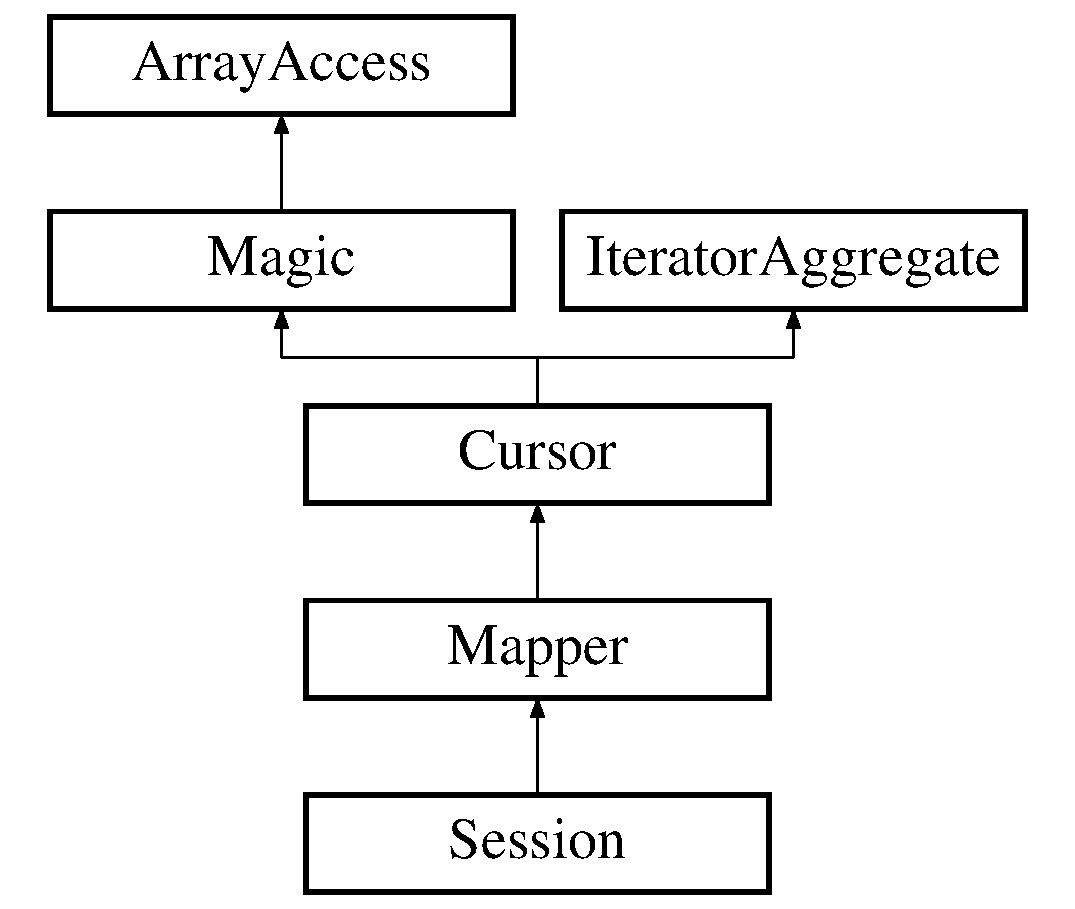
\includegraphics[height=5.000000cm]{class_d_b_1_1_s_q_l_1_1_session}
\end{center}
\end{figure}
\subsection*{Public Member Functions}
\begin{DoxyCompactItemize}
\item 
\hyperlink{class_d_b_1_1_s_q_l_1_1_session_a037c59224bcb347b69ca61df88ef7230}{open} (\$path, \$\hyperlink{class_d_b_1_1_s_q_l_a4b516aaa5fa38da4fed24ab6001627e2}{name})
\item 
\hyperlink{class_d_b_1_1_s_q_l_1_1_session_aa69c8bf1f1dcf4e72552efff1fe3e87e}{close} ()
\item 
\hyperlink{class_d_b_1_1_s_q_l_1_1_session_afa59bebedda70c37b94c2efc35da83f3}{read} (\$id)
\item 
\hyperlink{class_d_b_1_1_s_q_l_1_1_session_a5f277b5f0e4e2154cddc9a3a0d2bf57d}{write} (\$id, \$data)
\item 
\hyperlink{class_d_b_1_1_s_q_l_1_1_session_a726fa8a4b4b187b9ca32ba427aac8137}{destroy} (\$id)
\item 
\hyperlink{class_d_b_1_1_s_q_l_1_1_session_a60b027eb0df6d42b8fe2ec8c93cfbbae}{cleanup} (\$max)
\item 
\hyperlink{class_d_b_1_1_s_q_l_1_1_session_a30b416c35150ab6bdde364f527f612bd}{sid} ()
\item 
\hyperlink{class_d_b_1_1_s_q_l_1_1_session_a048d24aa22a28f92f1f3a7e3d323f45e}{csrf} ()
\item 
\hyperlink{class_d_b_1_1_s_q_l_1_1_session_a197bae3714812901860bd006b00f91de}{ip} ()
\item 
\hyperlink{class_d_b_1_1_s_q_l_1_1_session_ab0b8b94527259f4aacdf1fd45411abfe}{stamp} ()
\item 
\hyperlink{class_d_b_1_1_s_q_l_1_1_session_a77f6a261d70e66c7b7273774832482dc}{agent} ()
\item 
\hyperlink{class_d_b_1_1_s_q_l_1_1_session_acfaeaa649a2bb634903b84ebbb1515f3}{\+\_\+\+\_\+construct} (\textbackslash{}\hyperlink{class_d_b_1_1_s_q_l}{D\+B\textbackslash{}\+S\+QL} \$db, \$\hyperlink{class_d_b_1_1_s_q_l_1_1_mapper_a5aa7b43c8ec77df216a71a27da0a321c}{table}=\textquotesingle{}sessions\textquotesingle{}, \$force=T\+R\+UE, \$onsuspect=N\+U\+LL, \$key=N\+U\+LL)
\end{DoxyCompactItemize}
\subsection*{Data Fields}
\begin{DoxyCompactItemize}
\item 
\hypertarget{class_d_b_1_1_s_q_l_1_1_session_a871411a78a77c508569c380dd06fdd51}{}\label{class_d_b_1_1_s_q_l_1_1_session_a871411a78a77c508569c380dd06fdd51} 
\hyperlink{class_d_b_1_1_s_q_l_1_1_session_a871411a78a77c508569c380dd06fdd51}{\$\+\_\+csrf}
\begin{DoxyCompactList}\small\item\em Anti-\/\+C\+S\+RF token. \end{DoxyCompactList}\item 
\hypertarget{class_d_b_1_1_s_q_l_1_1_session_a7e43e09863a494197e0cdbf3f98c2ff5}{}\label{class_d_b_1_1_s_q_l_1_1_session_a7e43e09863a494197e0cdbf3f98c2ff5} 
\hyperlink{class_d_b_1_1_s_q_l_1_1_session_a7e43e09863a494197e0cdbf3f98c2ff5}{\$\+\_\+agent}
\begin{DoxyCompactList}\small\item\em User agent. \end{DoxyCompactList}\item 
\hypertarget{class_d_b_1_1_s_q_l_1_1_session_ac275a475a83ee8de16cf9c9f928fbe77}{}\label{class_d_b_1_1_s_q_l_1_1_session_ac275a475a83ee8de16cf9c9f928fbe77} 
\hyperlink{class_d_b_1_1_s_q_l_1_1_session_ac275a475a83ee8de16cf9c9f928fbe77}{\$\+\_\+ip}
\begin{DoxyCompactList}\small\item\em IP,. \end{DoxyCompactList}\item 
\hypertarget{class_d_b_1_1_s_q_l_1_1_session_ad96efa4953d3355e4c1aabc5cebad482}{}\label{class_d_b_1_1_s_q_l_1_1_session_ad96efa4953d3355e4c1aabc5cebad482} 
\hyperlink{class_d_b_1_1_s_q_l_1_1_session_ad96efa4953d3355e4c1aabc5cebad482}{\$onsuspect}
\begin{DoxyCompactList}\small\item\em Suspect callback. \end{DoxyCompactList}\end{DoxyCompactItemize}
\subsection*{Protected Attributes}
\begin{DoxyCompactItemize}
\item 
\hypertarget{class_d_b_1_1_s_q_l_1_1_session_a3b4e4b29ac1d6699dd65f8f0d6fa4133}{}\label{class_d_b_1_1_s_q_l_1_1_session_a3b4e4b29ac1d6699dd65f8f0d6fa4133} 
\hyperlink{class_d_b_1_1_s_q_l_1_1_session_a3b4e4b29ac1d6699dd65f8f0d6fa4133}{\$sid}
\begin{DoxyCompactList}\small\item\em \hyperlink{class_d_b_1_1_s_q_l_1_1_session}{Session} ID. \end{DoxyCompactList}\end{DoxyCompactItemize}
\subsection*{Additional Inherited Members}


\subsection{Detailed Description}
S\+Q\+L-\/managed session handler. 

Definition at line 26 of file session.\+php.



\subsection{Constructor \& Destructor Documentation}
\hypertarget{class_d_b_1_1_s_q_l_1_1_session_acfaeaa649a2bb634903b84ebbb1515f3}{}\label{class_d_b_1_1_s_q_l_1_1_session_acfaeaa649a2bb634903b84ebbb1515f3} 
\index{D\+B\+::\+S\+Q\+L\+::\+Session@{D\+B\+::\+S\+Q\+L\+::\+Session}!\+\_\+\+\_\+construct@{\+\_\+\+\_\+construct}}
\index{\+\_\+\+\_\+construct@{\+\_\+\+\_\+construct}!D\+B\+::\+S\+Q\+L\+::\+Session@{D\+B\+::\+S\+Q\+L\+::\+Session}}
\subsubsection{\texorpdfstring{\+\_\+\+\_\+construct()}{\_\_construct()}}
{\footnotesize\ttfamily \+\_\+\+\_\+construct (\begin{DoxyParamCaption}\item[{\textbackslash{}\hyperlink{class_d_b_1_1_s_q_l}{D\+B\textbackslash{}\+S\+QL}}]{\$db,  }\item[{}]{\$table = {\ttfamily \textquotesingle{}sessions\textquotesingle{}},  }\item[{}]{\$force = {\ttfamily TRUE},  }\item[{}]{\$onsuspect = {\ttfamily NULL},  }\item[{}]{\$key = {\ttfamily NULL} }\end{DoxyParamCaption})}

Instantiate class 
\begin{DoxyParams}{Parameters}
{\em \$db} & \\
\hline
{\em \$table} & string \\
\hline
{\em \$force} & bool \\
\hline
{\em \$onsuspect} & callback \\
\hline
{\em \$key} & string \\
\hline
\end{DoxyParams}


Definition at line 169 of file session.\+php.



\subsection{Member Function Documentation}
\hypertarget{class_d_b_1_1_s_q_l_1_1_session_a77f6a261d70e66c7b7273774832482dc}{}\label{class_d_b_1_1_s_q_l_1_1_session_a77f6a261d70e66c7b7273774832482dc} 
\index{D\+B\+::\+S\+Q\+L\+::\+Session@{D\+B\+::\+S\+Q\+L\+::\+Session}!agent@{agent}}
\index{agent@{agent}!D\+B\+::\+S\+Q\+L\+::\+Session@{D\+B\+::\+S\+Q\+L\+::\+Session}}
\subsubsection{\texorpdfstring{agent()}{agent()}}
{\footnotesize\ttfamily agent (\begin{DoxyParamCaption}{ }\end{DoxyParamCaption})}

Return H\+T\+TP user agent \begin{DoxyReturn}{Returns}
string 
\end{DoxyReturn}


Definition at line 157 of file session.\+php.

\hypertarget{class_d_b_1_1_s_q_l_1_1_session_a60b027eb0df6d42b8fe2ec8c93cfbbae}{}\label{class_d_b_1_1_s_q_l_1_1_session_a60b027eb0df6d42b8fe2ec8c93cfbbae} 
\index{D\+B\+::\+S\+Q\+L\+::\+Session@{D\+B\+::\+S\+Q\+L\+::\+Session}!cleanup@{cleanup}}
\index{cleanup@{cleanup}!D\+B\+::\+S\+Q\+L\+::\+Session@{D\+B\+::\+S\+Q\+L\+::\+Session}}
\subsubsection{\texorpdfstring{cleanup()}{cleanup()}}
{\footnotesize\ttfamily cleanup (\begin{DoxyParamCaption}\item[{}]{\$max }\end{DoxyParamCaption})}

Garbage collector \begin{DoxyReturn}{Returns}
T\+R\+UE 
\end{DoxyReturn}

\begin{DoxyParams}{Parameters}
{\em \$max} & int \\
\hline
\end{DoxyParams}


Definition at line 114 of file session.\+php.

\hypertarget{class_d_b_1_1_s_q_l_1_1_session_aa69c8bf1f1dcf4e72552efff1fe3e87e}{}\label{class_d_b_1_1_s_q_l_1_1_session_aa69c8bf1f1dcf4e72552efff1fe3e87e} 
\index{D\+B\+::\+S\+Q\+L\+::\+Session@{D\+B\+::\+S\+Q\+L\+::\+Session}!close@{close}}
\index{close@{close}!D\+B\+::\+S\+Q\+L\+::\+Session@{D\+B\+::\+S\+Q\+L\+::\+Session}}
\subsubsection{\texorpdfstring{close()}{close()}}
{\footnotesize\ttfamily close (\begin{DoxyParamCaption}{ }\end{DoxyParamCaption})}

Close session \begin{DoxyReturn}{Returns}
T\+R\+UE 
\end{DoxyReturn}


Definition at line 54 of file session.\+php.

\hypertarget{class_d_b_1_1_s_q_l_1_1_session_a048d24aa22a28f92f1f3a7e3d323f45e}{}\label{class_d_b_1_1_s_q_l_1_1_session_a048d24aa22a28f92f1f3a7e3d323f45e} 
\index{D\+B\+::\+S\+Q\+L\+::\+Session@{D\+B\+::\+S\+Q\+L\+::\+Session}!csrf@{csrf}}
\index{csrf@{csrf}!D\+B\+::\+S\+Q\+L\+::\+Session@{D\+B\+::\+S\+Q\+L\+::\+Session}}
\subsubsection{\texorpdfstring{csrf()}{csrf()}}
{\footnotesize\ttfamily csrf (\begin{DoxyParamCaption}{ }\end{DoxyParamCaption})}

Return anti-\/\+C\+S\+RF token \begin{DoxyReturn}{Returns}
string 
\end{DoxyReturn}


Definition at line 131 of file session.\+php.

\hypertarget{class_d_b_1_1_s_q_l_1_1_session_a726fa8a4b4b187b9ca32ba427aac8137}{}\label{class_d_b_1_1_s_q_l_1_1_session_a726fa8a4b4b187b9ca32ba427aac8137} 
\index{D\+B\+::\+S\+Q\+L\+::\+Session@{D\+B\+::\+S\+Q\+L\+::\+Session}!destroy@{destroy}}
\index{destroy@{destroy}!D\+B\+::\+S\+Q\+L\+::\+Session@{D\+B\+::\+S\+Q\+L\+::\+Session}}
\subsubsection{\texorpdfstring{destroy()}{destroy()}}
{\footnotesize\ttfamily destroy (\begin{DoxyParamCaption}\item[{}]{\$id }\end{DoxyParamCaption})}

Destroy session \begin{DoxyReturn}{Returns}
T\+R\+UE 
\end{DoxyReturn}

\begin{DoxyParams}{Parameters}
{\em \$id} & string \\
\hline
\end{DoxyParams}


Definition at line 104 of file session.\+php.

\hypertarget{class_d_b_1_1_s_q_l_1_1_session_a197bae3714812901860bd006b00f91de}{}\label{class_d_b_1_1_s_q_l_1_1_session_a197bae3714812901860bd006b00f91de} 
\index{D\+B\+::\+S\+Q\+L\+::\+Session@{D\+B\+::\+S\+Q\+L\+::\+Session}!ip@{ip}}
\index{ip@{ip}!D\+B\+::\+S\+Q\+L\+::\+Session@{D\+B\+::\+S\+Q\+L\+::\+Session}}
\subsubsection{\texorpdfstring{ip()}{ip()}}
{\footnotesize\ttfamily ip (\begin{DoxyParamCaption}{ }\end{DoxyParamCaption})}

Return IP address \begin{DoxyReturn}{Returns}
string 
\end{DoxyReturn}


Definition at line 139 of file session.\+php.

\hypertarget{class_d_b_1_1_s_q_l_1_1_session_a037c59224bcb347b69ca61df88ef7230}{}\label{class_d_b_1_1_s_q_l_1_1_session_a037c59224bcb347b69ca61df88ef7230} 
\index{D\+B\+::\+S\+Q\+L\+::\+Session@{D\+B\+::\+S\+Q\+L\+::\+Session}!open@{open}}
\index{open@{open}!D\+B\+::\+S\+Q\+L\+::\+Session@{D\+B\+::\+S\+Q\+L\+::\+Session}}
\subsubsection{\texorpdfstring{open()}{open()}}
{\footnotesize\ttfamily open (\begin{DoxyParamCaption}\item[{}]{\$path,  }\item[{}]{\$name }\end{DoxyParamCaption})}

Open session \begin{DoxyReturn}{Returns}
T\+R\+UE 
\end{DoxyReturn}

\begin{DoxyParams}{Parameters}
{\em \$path} & string \\
\hline
{\em \$name} & string \\
\hline
\end{DoxyParams}


Definition at line 46 of file session.\+php.

\hypertarget{class_d_b_1_1_s_q_l_1_1_session_afa59bebedda70c37b94c2efc35da83f3}{}\label{class_d_b_1_1_s_q_l_1_1_session_afa59bebedda70c37b94c2efc35da83f3} 
\index{D\+B\+::\+S\+Q\+L\+::\+Session@{D\+B\+::\+S\+Q\+L\+::\+Session}!read@{read}}
\index{read@{read}!D\+B\+::\+S\+Q\+L\+::\+Session@{D\+B\+::\+S\+Q\+L\+::\+Session}}
\subsubsection{\texorpdfstring{read()}{read()}}
{\footnotesize\ttfamily read (\begin{DoxyParamCaption}\item[{}]{\$id }\end{DoxyParamCaption})}

Return session data in serialized format \begin{DoxyReturn}{Returns}
string$\vert$\+F\+A\+L\+SE 
\end{DoxyReturn}

\begin{DoxyParams}{Parameters}
{\em \$id} & string \\
\hline
\end{DoxyParams}


Definition at line 65 of file session.\+php.

\hypertarget{class_d_b_1_1_s_q_l_1_1_session_a30b416c35150ab6bdde364f527f612bd}{}\label{class_d_b_1_1_s_q_l_1_1_session_a30b416c35150ab6bdde364f527f612bd} 
\index{D\+B\+::\+S\+Q\+L\+::\+Session@{D\+B\+::\+S\+Q\+L\+::\+Session}!sid@{sid}}
\index{sid@{sid}!D\+B\+::\+S\+Q\+L\+::\+Session@{D\+B\+::\+S\+Q\+L\+::\+Session}}
\subsubsection{\texorpdfstring{sid()}{sid()}}
{\footnotesize\ttfamily sid (\begin{DoxyParamCaption}{ }\end{DoxyParamCaption})}

Return session id (if session has started) \begin{DoxyReturn}{Returns}
string$\vert$\+N\+U\+LL 
\end{DoxyReturn}


Definition at line 123 of file session.\+php.

\hypertarget{class_d_b_1_1_s_q_l_1_1_session_ab0b8b94527259f4aacdf1fd45411abfe}{}\label{class_d_b_1_1_s_q_l_1_1_session_ab0b8b94527259f4aacdf1fd45411abfe} 
\index{D\+B\+::\+S\+Q\+L\+::\+Session@{D\+B\+::\+S\+Q\+L\+::\+Session}!stamp@{stamp}}
\index{stamp@{stamp}!D\+B\+::\+S\+Q\+L\+::\+Session@{D\+B\+::\+S\+Q\+L\+::\+Session}}
\subsubsection{\texorpdfstring{stamp()}{stamp()}}
{\footnotesize\ttfamily stamp (\begin{DoxyParamCaption}{ }\end{DoxyParamCaption})}

Return Unix timestamp \begin{DoxyReturn}{Returns}
string$\vert$\+F\+A\+L\+SE 
\end{DoxyReturn}


Definition at line 147 of file session.\+php.

\hypertarget{class_d_b_1_1_s_q_l_1_1_session_a5f277b5f0e4e2154cddc9a3a0d2bf57d}{}\label{class_d_b_1_1_s_q_l_1_1_session_a5f277b5f0e4e2154cddc9a3a0d2bf57d} 
\index{D\+B\+::\+S\+Q\+L\+::\+Session@{D\+B\+::\+S\+Q\+L\+::\+Session}!write@{write}}
\index{write@{write}!D\+B\+::\+S\+Q\+L\+::\+Session@{D\+B\+::\+S\+Q\+L\+::\+Session}}
\subsubsection{\texorpdfstring{write()}{write()}}
{\footnotesize\ttfamily write (\begin{DoxyParamCaption}\item[{}]{\$id,  }\item[{}]{\$data }\end{DoxyParamCaption})}

Write session data \begin{DoxyReturn}{Returns}
T\+R\+UE 
\end{DoxyReturn}

\begin{DoxyParams}{Parameters}
{\em \$id} & string \\
\hline
{\em \$data} & string \\
\hline
\end{DoxyParams}


Definition at line 89 of file session.\+php.



The documentation for this class was generated from the following file\+:\begin{DoxyCompactItemize}
\item 
/\+Users/aplennevaux/\+G\+I\+T\+H\+U\+B/\+Visionary-\/website/src/vendor/bcosca/fatfree/lib/db/sql/session.\+php\end{DoxyCompactItemize}

\hypertarget{class_s_m_t_p}{}\section{S\+M\+TP Class Reference}
\label{class_s_m_t_p}\index{S\+M\+TP@{S\+M\+TP}}


\hyperlink{class_s_m_t_p}{S\+M\+TP} plug-\/in.  


Inheritance diagram for S\+M\+TP\+:\begin{figure}[H]
\begin{center}
\leavevmode
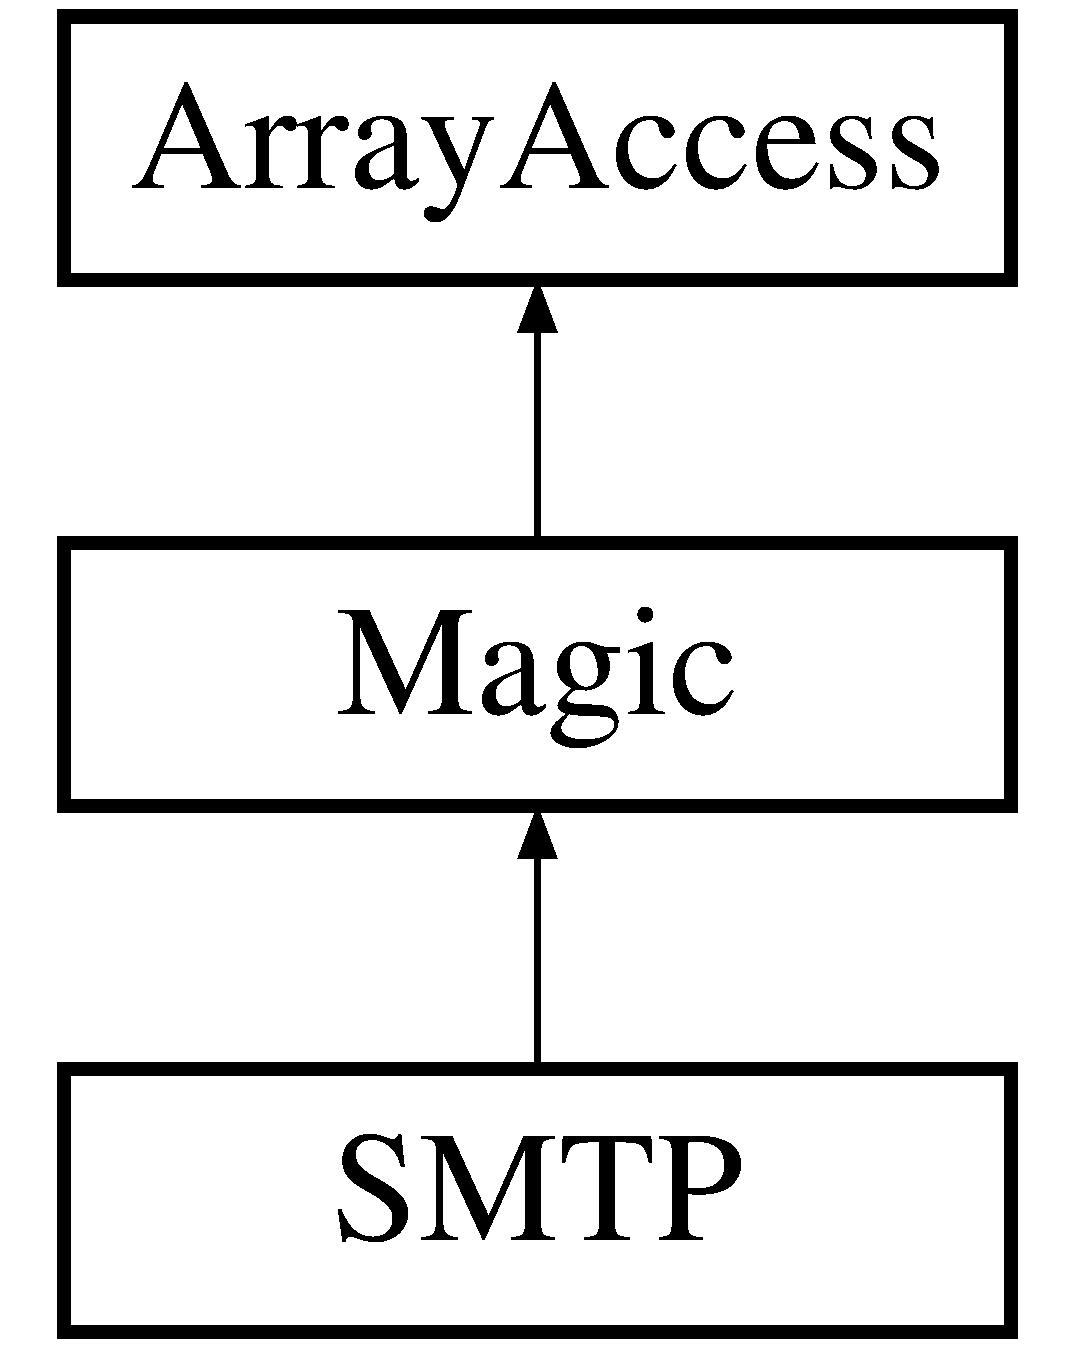
\includegraphics[height=3.000000cm]{class_s_m_t_p}
\end{center}
\end{figure}
\subsection*{Public Member Functions}
\begin{DoxyCompactItemize}
\item 
\hyperlink{class_s_m_t_p_ace1ae5be37bf26c172cc7ea4e1a65e26}{exists} (\$key)
\item 
\hyperlink{class_s_m_t_p_ac8d8012023e560c81f55a629022cb65a}{set} (\$key, \$val)
\item 
\& \hyperlink{class_s_m_t_p_ac3695923790b06917410e205068b8376}{get} (\$key)
\item 
\hyperlink{class_s_m_t_p_a10a949ef75de6c82c98ac555f371ba83}{clear} (\$key)
\item 
\hyperlink{class_s_m_t_p_a5e06d9b7f0033278f40a41d081efbe71}{log} ()
\item 
\hyperlink{class_s_m_t_p_acddb7c5e0234289640206f7ee89c14e5}{attach} (\$file, \$alias=N\+U\+LL, \$cid=N\+U\+LL)
\item 
\hyperlink{class_s_m_t_p_acf11a2bd1ca8c23866ccadfbe1e0954d}{send} (\$message, \$\hyperlink{class_s_m_t_p_a5e06d9b7f0033278f40a41d081efbe71}{log}=T\+R\+UE, \$mock=F\+A\+L\+SE)
\item 
\hyperlink{class_s_m_t_p_ad7de317dd2066f6724c0a560b6791543}{\+\_\+\+\_\+construct} ( \$host=\textquotesingle{}localhost\textquotesingle{}, \$port=25, \$scheme=N\+U\+LL, \$user=N\+U\+LL, \$pw=N\+U\+LL)
\end{DoxyCompactItemize}
\subsection*{Data Fields}
\begin{DoxyCompactItemize}
\item 
\hypertarget{class_s_m_t_p_aa2f80297e973639eba0f2f8619fe783b}{}\label{class_s_m_t_p_aa2f80297e973639eba0f2f8619fe783b} 
\hyperlink{class_s_m_t_p_aa2f80297e973639eba0f2f8619fe783b}{\$attachments}
\begin{DoxyCompactList}\small\item\em E-\/mail attachments. \end{DoxyCompactList}\item 
\hypertarget{class_s_m_t_p_a711797613cb863ca0756df789c396bf2}{}\label{class_s_m_t_p_a711797613cb863ca0756df789c396bf2} 
\hyperlink{class_s_m_t_p_a711797613cb863ca0756df789c396bf2}{\$host}
\begin{DoxyCompactList}\small\item\em \hyperlink{class_s_m_t_p}{S\+M\+TP} host. \end{DoxyCompactList}\item 
\hypertarget{class_s_m_t_p_aa0787efab4b22e8a212882f3409d4c77}{}\label{class_s_m_t_p_aa0787efab4b22e8a212882f3409d4c77} 
\hyperlink{class_s_m_t_p_aa0787efab4b22e8a212882f3409d4c77}{\$port}
\begin{DoxyCompactList}\small\item\em \hyperlink{class_s_m_t_p}{S\+M\+TP} port. \end{DoxyCompactList}\item 
\hypertarget{class_s_m_t_p_a1665950e3e3b63a02fc5a48706ac81c4}{}\label{class_s_m_t_p_a1665950e3e3b63a02fc5a48706ac81c4} 
\hyperlink{class_s_m_t_p_a1665950e3e3b63a02fc5a48706ac81c4}{\$scheme}
\begin{DoxyCompactList}\small\item\em T\+L\+S/\+S\+SL. \end{DoxyCompactList}\item 
\hypertarget{class_s_m_t_p_a598ca4e71b15a1313ec95f0df1027ca5}{}\label{class_s_m_t_p_a598ca4e71b15a1313ec95f0df1027ca5} 
\hyperlink{class_s_m_t_p_a598ca4e71b15a1313ec95f0df1027ca5}{\$user}
\begin{DoxyCompactList}\small\item\em User ID. \end{DoxyCompactList}\item 
\hypertarget{class_s_m_t_p_a4a84bb9d73addd9e90f2f34c36035df4}{}\label{class_s_m_t_p_a4a84bb9d73addd9e90f2f34c36035df4} 
\hyperlink{class_s_m_t_p_a4a84bb9d73addd9e90f2f34c36035df4}{\$pw}
\begin{DoxyCompactList}\small\item\em Password. \end{DoxyCompactList}\item 
\hypertarget{class_s_m_t_p_a33a9dcf5eaeebf833f2390060f8caf5e}{}\label{class_s_m_t_p_a33a9dcf5eaeebf833f2390060f8caf5e} 
\hyperlink{class_s_m_t_p_a33a9dcf5eaeebf833f2390060f8caf5e}{\$socket}
\begin{DoxyCompactList}\small\item\em T\+C\+P/\+IP socket. \end{DoxyCompactList}\item 
\hypertarget{class_s_m_t_p_a9a2cf15a653aee8be437f7ae474cd494}{}\label{class_s_m_t_p_a9a2cf15a653aee8be437f7ae474cd494} 
\hyperlink{class_s_m_t_p_a9a2cf15a653aee8be437f7ae474cd494}{\$log}
\begin{DoxyCompactList}\small\item\em Server-\/client conversation. \end{DoxyCompactList}\end{DoxyCompactItemize}
{\bf }\par
\begin{DoxyCompactItemize}
\item 
\hypertarget{class_s_m_t_p_a3ea1a09993798da7eba3b05e89fca4c2}{}\label{class_s_m_t_p_a3ea1a09993798da7eba3b05e89fca4c2} 
const {\bfseries E\+\_\+\+Header} =\textquotesingle{}\%s\+: header is required\textquotesingle{}
\item 
\hypertarget{class_s_m_t_p_ae837eb485f6bf62b8bbe8e9007c04cb2}{}\label{class_s_m_t_p_ae837eb485f6bf62b8bbe8e9007c04cb2} 
const {\bfseries E\+\_\+\+Blank} =\textquotesingle{}Message must not be blank\textquotesingle{}
\item 
\hypertarget{class_s_m_t_p_aedc0129d8cb1011801aee1950c279caf}{}\label{class_s_m_t_p_aedc0129d8cb1011801aee1950c279caf} 
const {\bfseries E\+\_\+\+Attach} =\textquotesingle{}Attachment \%s not found\textquotesingle{}
\end{DoxyCompactItemize}

\subsection*{Protected Member Functions}
\begin{DoxyCompactItemize}
\item 
\hyperlink{class_s_m_t_p_afee77a9b8498c6a0875b75ae7313e545}{fixheader} (\$key)
\item 
\hyperlink{class_s_m_t_p_ab57e2499b18f17f0cf67e12d546ad225}{dialog} (\$cmd=N\+U\+LL, \$\hyperlink{class_s_m_t_p_a5e06d9b7f0033278f40a41d081efbe71}{log}=T\+R\+UE, \$mock=F\+A\+L\+SE)
\end{DoxyCompactItemize}
\subsection*{Protected Attributes}
\begin{DoxyCompactItemize}
\item 
\hypertarget{class_s_m_t_p_a52500036ee807241b8b4b7e2367c49ef}{}\label{class_s_m_t_p_a52500036ee807241b8b4b7e2367c49ef} 
\hyperlink{class_s_m_t_p_a52500036ee807241b8b4b7e2367c49ef}{\$headers}
\begin{DoxyCompactList}\small\item\em Message properties. \end{DoxyCompactList}\end{DoxyCompactItemize}


\subsection{Detailed Description}
\hyperlink{class_s_m_t_p}{S\+M\+TP} plug-\/in. 

Definition at line 24 of file smtp.\+php.



\subsection{Constructor \& Destructor Documentation}
\hypertarget{class_s_m_t_p_ad7de317dd2066f6724c0a560b6791543}{}\label{class_s_m_t_p_ad7de317dd2066f6724c0a560b6791543} 
\index{S\+M\+TP@{S\+M\+TP}!\+\_\+\+\_\+construct@{\+\_\+\+\_\+construct}}
\index{\+\_\+\+\_\+construct@{\+\_\+\+\_\+construct}!S\+M\+TP@{S\+M\+TP}}
\subsubsection{\texorpdfstring{\+\_\+\+\_\+construct()}{\_\_construct()}}
{\footnotesize\ttfamily \+\_\+\+\_\+construct (\begin{DoxyParamCaption}\item[{}]{\$host = {\ttfamily \textquotesingle{}localhost\textquotesingle{}},  }\item[{}]{\$port = {\ttfamily 25},  }\item[{}]{\$scheme = {\ttfamily NULL},  }\item[{}]{\$user = {\ttfamily NULL},  }\item[{}]{\$pw = {\ttfamily NULL} }\end{DoxyParamCaption})}

Instantiate class 
\begin{DoxyParams}{Parameters}
{\em \$host} & string \\
\hline
{\em \$port} & int \\
\hline
{\em \$scheme} & string \\
\hline
{\em \$user} & string \\
\hline
{\em \$pw} & string \\
\hline
\end{DoxyParams}


Definition at line 338 of file smtp.\+php.



\subsection{Member Function Documentation}
\hypertarget{class_s_m_t_p_acddb7c5e0234289640206f7ee89c14e5}{}\label{class_s_m_t_p_acddb7c5e0234289640206f7ee89c14e5} 
\index{S\+M\+TP@{S\+M\+TP}!attach@{attach}}
\index{attach@{attach}!S\+M\+TP@{S\+M\+TP}}
\subsubsection{\texorpdfstring{attach()}{attach()}}
{\footnotesize\ttfamily attach (\begin{DoxyParamCaption}\item[{}]{\$file,  }\item[{}]{\$alias = {\ttfamily NULL},  }\item[{}]{\$cid = {\ttfamily NULL} }\end{DoxyParamCaption})}

Add e-\/mail attachment \begin{DoxyReturn}{Returns}
N\+U\+LL 
\end{DoxyReturn}

\begin{DoxyParams}{Parameters}
{\em \$file} & string \\
\hline
{\em \$alias} & string \\
\hline
{\em \$cid} & string \\
\hline
\end{DoxyParams}


Definition at line 168 of file smtp.\+php.

\hypertarget{class_s_m_t_p_a10a949ef75de6c82c98ac555f371ba83}{}\label{class_s_m_t_p_a10a949ef75de6c82c98ac555f371ba83} 
\index{S\+M\+TP@{S\+M\+TP}!clear@{clear}}
\index{clear@{clear}!S\+M\+TP@{S\+M\+TP}}
\subsubsection{\texorpdfstring{clear()}{clear()}}
{\footnotesize\ttfamily clear (\begin{DoxyParamCaption}\item[{}]{\$key }\end{DoxyParamCaption})}

Remove header \begin{DoxyReturn}{Returns}
N\+U\+LL 
\end{DoxyReturn}

\begin{DoxyParams}{Parameters}
{\em \$key} & string \\
\hline
\end{DoxyParams}


Definition at line 103 of file smtp.\+php.

\hypertarget{class_s_m_t_p_ab57e2499b18f17f0cf67e12d546ad225}{}\label{class_s_m_t_p_ab57e2499b18f17f0cf67e12d546ad225} 
\index{S\+M\+TP@{S\+M\+TP}!dialog@{dialog}}
\index{dialog@{dialog}!S\+M\+TP@{S\+M\+TP}}
\subsubsection{\texorpdfstring{dialog()}{dialog()}}
{\footnotesize\ttfamily dialog (\begin{DoxyParamCaption}\item[{}]{\$cmd = {\ttfamily NULL},  }\item[{}]{\$log = {\ttfamily TRUE},  }\item[{}]{\$mock = {\ttfamily FALSE} }\end{DoxyParamCaption})\hspace{0.3cm}{\ttfamily [protected]}}

Send \hyperlink{class_s_m_t_p}{S\+M\+TP} command and record server response \begin{DoxyReturn}{Returns}
string 
\end{DoxyReturn}

\begin{DoxyParams}{Parameters}
{\em \$cmd} & string \\
\hline
{\em \$log} & bool \\
\hline
{\em \$mock} & bool \\
\hline
\end{DoxyParams}


Definition at line 123 of file smtp.\+php.

\hypertarget{class_s_m_t_p_ace1ae5be37bf26c172cc7ea4e1a65e26}{}\label{class_s_m_t_p_ace1ae5be37bf26c172cc7ea4e1a65e26} 
\index{S\+M\+TP@{S\+M\+TP}!exists@{exists}}
\index{exists@{exists}!S\+M\+TP@{S\+M\+TP}}
\subsubsection{\texorpdfstring{exists()}{exists()}}
{\footnotesize\ttfamily exists (\begin{DoxyParamCaption}\item[{}]{\$key }\end{DoxyParamCaption})}

Return T\+R\+UE if header exists \begin{DoxyReturn}{Returns}
bool 
\end{DoxyReturn}

\begin{DoxyParams}{Parameters}
{\em \$key} & \\
\hline
\end{DoxyParams}


Definition at line 68 of file smtp.\+php.

\hypertarget{class_s_m_t_p_afee77a9b8498c6a0875b75ae7313e545}{}\label{class_s_m_t_p_afee77a9b8498c6a0875b75ae7313e545} 
\index{S\+M\+TP@{S\+M\+TP}!fixheader@{fixheader}}
\index{fixheader@{fixheader}!S\+M\+TP@{S\+M\+TP}}
\subsubsection{\texorpdfstring{fixheader()}{fixheader()}}
{\footnotesize\ttfamily fixheader (\begin{DoxyParamCaption}\item[{}]{\$key }\end{DoxyParamCaption})\hspace{0.3cm}{\ttfamily [protected]}}

Fix header \begin{DoxyReturn}{Returns}
string 
\end{DoxyReturn}

\begin{DoxyParams}{Parameters}
{\em \$key} & string \\
\hline
\end{DoxyParams}


Definition at line 58 of file smtp.\+php.

\hypertarget{class_s_m_t_p_ac3695923790b06917410e205068b8376}{}\label{class_s_m_t_p_ac3695923790b06917410e205068b8376} 
\index{S\+M\+TP@{S\+M\+TP}!get@{get}}
\index{get@{get}!S\+M\+TP@{S\+M\+TP}}
\subsubsection{\texorpdfstring{get()}{get()}}
{\footnotesize\ttfamily \& get (\begin{DoxyParamCaption}\item[{}]{\$key }\end{DoxyParamCaption})}

Return value of e-\/mail header \begin{DoxyReturn}{Returns}
string$\vert$\+N\+U\+LL 
\end{DoxyReturn}

\begin{DoxyParams}{Parameters}
{\em \$key} & string \\
\hline
\end{DoxyParams}


Definition at line 89 of file smtp.\+php.

\hypertarget{class_s_m_t_p_a5e06d9b7f0033278f40a41d081efbe71}{}\label{class_s_m_t_p_a5e06d9b7f0033278f40a41d081efbe71} 
\index{S\+M\+TP@{S\+M\+TP}!log@{log}}
\index{log@{log}!S\+M\+TP@{S\+M\+TP}}
\subsubsection{\texorpdfstring{log()}{log()}}
{\footnotesize\ttfamily log (\begin{DoxyParamCaption}{ }\end{DoxyParamCaption})}

Return client-\/server conversation history \begin{DoxyReturn}{Returns}
string 
\end{DoxyReturn}


Definition at line 112 of file smtp.\+php.

\hypertarget{class_s_m_t_p_acf11a2bd1ca8c23866ccadfbe1e0954d}{}\label{class_s_m_t_p_acf11a2bd1ca8c23866ccadfbe1e0954d} 
\index{S\+M\+TP@{S\+M\+TP}!send@{send}}
\index{send@{send}!S\+M\+TP@{S\+M\+TP}}
\subsubsection{\texorpdfstring{send()}{send()}}
{\footnotesize\ttfamily send (\begin{DoxyParamCaption}\item[{}]{\$message,  }\item[{}]{\$log = {\ttfamily TRUE},  }\item[{}]{\$mock = {\ttfamily FALSE} }\end{DoxyParamCaption})}

Transmit message \begin{DoxyReturn}{Returns}
bool 
\end{DoxyReturn}

\begin{DoxyParams}{Parameters}
{\em \$message} & string \\
\hline
{\em \$log} & bool \\
\hline
{\em \$mock} & bool \\
\hline
\end{DoxyParams}


Definition at line 183 of file smtp.\+php.

\hypertarget{class_s_m_t_p_ac8d8012023e560c81f55a629022cb65a}{}\label{class_s_m_t_p_ac8d8012023e560c81f55a629022cb65a} 
\index{S\+M\+TP@{S\+M\+TP}!set@{set}}
\index{set@{set}!S\+M\+TP@{S\+M\+TP}}
\subsubsection{\texorpdfstring{set()}{set()}}
{\footnotesize\ttfamily set (\begin{DoxyParamCaption}\item[{}]{\$key,  }\item[{}]{\$val }\end{DoxyParamCaption})}

Bind value to e-\/mail header \begin{DoxyReturn}{Returns}
string 
\end{DoxyReturn}

\begin{DoxyParams}{Parameters}
{\em \$key} & string \\
\hline
{\em \$val} & string \\
\hline
\end{DoxyParams}


Definition at line 79 of file smtp.\+php.



The documentation for this class was generated from the following file\+:\begin{DoxyCompactItemize}
\item 
/\+Users/aplennevaux/\+G\+I\+T\+H\+U\+B/\+Visionary-\/website/src/vendor/bcosca/fatfree/lib/smtp.\+php\end{DoxyCompactItemize}

\hypertarget{class_d_b_1_1_s_q_l}{}\section{S\+QL Class Reference}
\label{class_d_b_1_1_s_q_l}\index{S\+QL@{S\+QL}}


P\+DO wrapper.  


\subsection*{Public Member Functions}
\begin{DoxyCompactItemize}
\item 
\hyperlink{class_d_b_1_1_s_q_l_a3a9793666e688407121d76d3a7e4db5d}{begin} ()
\item 
\hyperlink{class_d_b_1_1_s_q_l_afa549adf79e3f8c09fe8f903dd5fbfa7}{rollback} ()
\item 
\hyperlink{class_d_b_1_1_s_q_l_af5674c27d4a92f6228565010eacbb9cb}{commit} ()
\item 
\hyperlink{class_d_b_1_1_s_q_l_aeb7a9cfb4d43f94280b9c261ebb06148}{trans} ()
\item 
\hyperlink{class_d_b_1_1_s_q_l_a6fde55847377176e4f51ddd53705f269}{type} (\$val)
\item 
\hyperlink{class_d_b_1_1_s_q_l_a2f2c81ec59416b46db04db19ac4f8e1c}{value} (\$\hyperlink{class_d_b_1_1_s_q_l_a6fde55847377176e4f51ddd53705f269}{type}, \$val)
\item 
\hyperlink{class_d_b_1_1_s_q_l_a5fada1d189c38aeffb28fb712669309f}{exec} (\$cmds, \$args=N\+U\+LL, \$ttl=0, \$\hyperlink{class_d_b_1_1_s_q_l_a92faa80a7077936bd630e5dcc7bb4a64}{log}=T\+R\+UE, \$stamp=F\+A\+L\+SE)
\item 
\hyperlink{class_d_b_1_1_s_q_l_ac751e87b3d4c4bf2feb03bee8b092755}{count} ()
\item 
\hyperlink{class_d_b_1_1_s_q_l_a92faa80a7077936bd630e5dcc7bb4a64}{log} (\$flag=T\+R\+UE)
\item 
\hyperlink{class_d_b_1_1_s_q_l_ab0c9a209aa19a69b7c94e20bd6e536b1}{schema} (\$table, \$fields=N\+U\+LL, \$ttl=0)
\item 
\hyperlink{class_d_b_1_1_s_q_l_a719a37ee06136f9b4a4214632466bfb1}{quote} (\$val, \$\hyperlink{class_d_b_1_1_s_q_l_a6fde55847377176e4f51ddd53705f269}{type}=\textbackslash{}P\+D\+O\+::\+P\+A\+R\+A\+M\+\_\+\+S\+TR)
\item 
\hyperlink{class_d_b_1_1_s_q_l_a0a684acda95e124d8596758e4986fe44}{uuid} ()
\item 
\hyperlink{class_d_b_1_1_s_q_l_aa7612909f2506ecd3f2bc4ecbef3fe31}{pdo} ()
\item 
\hyperlink{class_d_b_1_1_s_q_l_a050ad2e495e82f1399b484074dd4974d}{driver} ()
\item 
\hyperlink{class_d_b_1_1_s_q_l_a6080dae0886626b9a4cedb29240708b1}{version} ()
\item 
\hyperlink{class_d_b_1_1_s_q_l_a4b516aaa5fa38da4fed24ab6001627e2}{name} ()
\item 
\hyperlink{class_d_b_1_1_s_q_l_a7efb19068579d27341ed4361fca37eff}{quotekey} (\$key, \$split=T\+R\+UE)
\item 
\hyperlink{class_d_b_1_1_s_q_l_a975d2c46a134129eb727fadcadf48adf}{\+\_\+\+\_\+call} (\$func, array \$args)
\item 
\hyperlink{class_d_b_1_1_s_q_l_ae8468efbf3f6acec2855c63413e4251d}{\+\_\+\+\_\+construct} (\$dsn, \$user=N\+U\+LL, \$pw=N\+U\+LL, array \$options=N\+U\+LL)
\end{DoxyCompactItemize}
\subsection*{Data Fields}
\begin{DoxyCompactItemize}
\item 
\hypertarget{class_d_b_1_1_s_q_l_ae82417822cd5c7de57aa5816da1b922c}{}\label{class_d_b_1_1_s_q_l_ae82417822cd5c7de57aa5816da1b922c} 
const {\bfseries P\+A\+R\+A\+M\+\_\+\+F\+L\+O\+AT} =\textquotesingle{}float\textquotesingle{}
\item 
\hypertarget{class_d_b_1_1_s_q_l_a5766efd703cef0e00bfc06b3f3acbe0e}{}\label{class_d_b_1_1_s_q_l_a5766efd703cef0e00bfc06b3f3acbe0e} 
\hyperlink{class_d_b_1_1_s_q_l_a5766efd703cef0e00bfc06b3f3acbe0e}{\$pdo}
\begin{DoxyCompactList}\small\item\em Raw P\+DO. \end{DoxyCompactList}\item 
\hypertarget{class_d_b_1_1_s_q_l_a6441cca8c9fa11e16d2017e8cb733c10}{}\label{class_d_b_1_1_s_q_l_a6441cca8c9fa11e16d2017e8cb733c10} 
\hyperlink{class_d_b_1_1_s_q_l_a6441cca8c9fa11e16d2017e8cb733c10}{\$dsn}
\begin{DoxyCompactList}\small\item\em Data source name. \end{DoxyCompactList}\item 
\hypertarget{class_d_b_1_1_s_q_l_a8a3b012ad4844366d9207d8f0e174a00}{}\label{class_d_b_1_1_s_q_l_a8a3b012ad4844366d9207d8f0e174a00} 
\hyperlink{class_d_b_1_1_s_q_l_a8a3b012ad4844366d9207d8f0e174a00}{\$engine}
\begin{DoxyCompactList}\small\item\em Database engine. \end{DoxyCompactList}\item 
\hypertarget{class_d_b_1_1_s_q_l_ac5111a571fffa2499732833bb7f0d8c1}{}\label{class_d_b_1_1_s_q_l_ac5111a571fffa2499732833bb7f0d8c1} 
\hyperlink{class_d_b_1_1_s_q_l_ac5111a571fffa2499732833bb7f0d8c1}{\$dbname}
\begin{DoxyCompactList}\small\item\em Database name. \end{DoxyCompactList}\item 
\hypertarget{class_d_b_1_1_s_q_l_ac75852aae94b46848119a6d7c922cf2e}{}\label{class_d_b_1_1_s_q_l_ac75852aae94b46848119a6d7c922cf2e} 
\hyperlink{class_d_b_1_1_s_q_l_ac75852aae94b46848119a6d7c922cf2e}{\$trans} =F\+A\+L\+SE
\begin{DoxyCompactList}\small\item\em Transaction flag. \end{DoxyCompactList}\item 
\hypertarget{class_d_b_1_1_s_q_l_ace2ec39e7df3899fa8df9640ec274b03}{}\label{class_d_b_1_1_s_q_l_ace2ec39e7df3899fa8df9640ec274b03} 
\hyperlink{class_d_b_1_1_s_q_l_ace2ec39e7df3899fa8df9640ec274b03}{\$rows} =0
\begin{DoxyCompactList}\small\item\em Number of rows affected by query. \end{DoxyCompactList}\item 
\hypertarget{class_d_b_1_1_s_q_l_a9a2cf15a653aee8be437f7ae474cd494}{}\label{class_d_b_1_1_s_q_l_a9a2cf15a653aee8be437f7ae474cd494} 
\hyperlink{class_d_b_1_1_s_q_l_a9a2cf15a653aee8be437f7ae474cd494}{\$log}
\begin{DoxyCompactList}\small\item\em \hyperlink{class_d_b_1_1_s_q_l}{S\+QL} log. \end{DoxyCompactList}\end{DoxyCompactItemize}
{\bf }\par
\begin{DoxyCompactItemize}
\item 
\hypertarget{class_d_b_1_1_s_q_l_a11f97c3c297f2a5a6ed6fd92b78c8a74}{}\label{class_d_b_1_1_s_q_l_a11f97c3c297f2a5a6ed6fd92b78c8a74} 
const {\bfseries E\+\_\+\+P\+Key} =\textquotesingle{}Table \%s does not have a primary key\textquotesingle{}
\end{DoxyCompactItemize}

\subsection*{Protected Attributes}
\begin{DoxyCompactItemize}
\item 
\hypertarget{class_d_b_1_1_s_q_l_aeccc2a337445686487ea085278c79eff}{}\label{class_d_b_1_1_s_q_l_aeccc2a337445686487ea085278c79eff} 
\hyperlink{class_d_b_1_1_s_q_l_aeccc2a337445686487ea085278c79eff}{\$uuid}
\begin{DoxyCompactList}\small\item\em U\+U\+ID. \end{DoxyCompactList}\end{DoxyCompactItemize}


\subsection{Detailed Description}
P\+DO wrapper. 

Definition at line 26 of file sql.\+php.



\subsection{Constructor \& Destructor Documentation}
\hypertarget{class_d_b_1_1_s_q_l_ae8468efbf3f6acec2855c63413e4251d}{}\label{class_d_b_1_1_s_q_l_ae8468efbf3f6acec2855c63413e4251d} 
\index{D\+B\+::\+S\+QL@{D\+B\+::\+S\+QL}!\+\_\+\+\_\+construct@{\+\_\+\+\_\+construct}}
\index{\+\_\+\+\_\+construct@{\+\_\+\+\_\+construct}!D\+B\+::\+S\+QL@{D\+B\+::\+S\+QL}}
\subsubsection{\texorpdfstring{\+\_\+\+\_\+construct()}{\_\_construct()}}
{\footnotesize\ttfamily \+\_\+\+\_\+construct (\begin{DoxyParamCaption}\item[{}]{\$dsn,  }\item[{}]{\$user = {\ttfamily NULL},  }\item[{}]{\$pw = {\ttfamily NULL},  }\item[{array}]{\$options = {\ttfamily NULL} }\end{DoxyParamCaption})}

Instantiate class 
\begin{DoxyParams}{Parameters}
{\em \$dsn} & string \\
\hline
{\em \$user} & string \\
\hline
{\em \$pw} & string \\
\hline
{\em \$options} & array \\
\hline
\end{DoxyParams}


Definition at line 486 of file sql.\+php.



\subsection{Member Function Documentation}
\hypertarget{class_d_b_1_1_s_q_l_a975d2c46a134129eb727fadcadf48adf}{}\label{class_d_b_1_1_s_q_l_a975d2c46a134129eb727fadcadf48adf} 
\index{D\+B\+::\+S\+QL@{D\+B\+::\+S\+QL}!\+\_\+\+\_\+call@{\+\_\+\+\_\+call}}
\index{\+\_\+\+\_\+call@{\+\_\+\+\_\+call}!D\+B\+::\+S\+QL@{D\+B\+::\+S\+QL}}
\subsubsection{\texorpdfstring{\+\_\+\+\_\+call()}{\_\_call()}}
{\footnotesize\ttfamily \+\_\+\+\_\+call (\begin{DoxyParamCaption}\item[{}]{\$func,  }\item[{array}]{\$args }\end{DoxyParamCaption})}

Redirect call to P\+DO object \begin{DoxyReturn}{Returns}
mixed 
\end{DoxyReturn}

\begin{DoxyParams}{Parameters}
{\em \$func} & string \\
\hline
{\em \$args} & array \\
\hline
\end{DoxyParams}


Definition at line 471 of file sql.\+php.

\hypertarget{class_d_b_1_1_s_q_l_a3a9793666e688407121d76d3a7e4db5d}{}\label{class_d_b_1_1_s_q_l_a3a9793666e688407121d76d3a7e4db5d} 
\index{D\+B\+::\+S\+QL@{D\+B\+::\+S\+QL}!begin@{begin}}
\index{begin@{begin}!D\+B\+::\+S\+QL@{D\+B\+::\+S\+QL}}
\subsubsection{\texorpdfstring{begin()}{begin()}}
{\footnotesize\ttfamily begin (\begin{DoxyParamCaption}{ }\end{DoxyParamCaption})}

Begin \hyperlink{class_d_b_1_1_s_q_l}{S\+QL} transaction \begin{DoxyReturn}{Returns}
bool 
\end{DoxyReturn}


Definition at line 58 of file sql.\+php.

\hypertarget{class_d_b_1_1_s_q_l_af5674c27d4a92f6228565010eacbb9cb}{}\label{class_d_b_1_1_s_q_l_af5674c27d4a92f6228565010eacbb9cb} 
\index{D\+B\+::\+S\+QL@{D\+B\+::\+S\+QL}!commit@{commit}}
\index{commit@{commit}!D\+B\+::\+S\+QL@{D\+B\+::\+S\+QL}}
\subsubsection{\texorpdfstring{commit()}{commit()}}
{\footnotesize\ttfamily commit (\begin{DoxyParamCaption}{ }\end{DoxyParamCaption})}

Commit \hyperlink{class_d_b_1_1_s_q_l}{S\+QL} transaction \begin{DoxyReturn}{Returns}
bool 
\end{DoxyReturn}


Definition at line 78 of file sql.\+php.

\hypertarget{class_d_b_1_1_s_q_l_ac751e87b3d4c4bf2feb03bee8b092755}{}\label{class_d_b_1_1_s_q_l_ac751e87b3d4c4bf2feb03bee8b092755} 
\index{D\+B\+::\+S\+QL@{D\+B\+::\+S\+QL}!count@{count}}
\index{count@{count}!D\+B\+::\+S\+QL@{D\+B\+::\+S\+QL}}
\subsubsection{\texorpdfstring{count()}{count()}}
{\footnotesize\ttfamily count (\begin{DoxyParamCaption}{ }\end{DoxyParamCaption})}

Return number of rows affected by last query \begin{DoxyReturn}{Returns}
int 
\end{DoxyReturn}


Definition at line 277 of file sql.\+php.

\hypertarget{class_d_b_1_1_s_q_l_a050ad2e495e82f1399b484074dd4974d}{}\label{class_d_b_1_1_s_q_l_a050ad2e495e82f1399b484074dd4974d} 
\index{D\+B\+::\+S\+QL@{D\+B\+::\+S\+QL}!driver@{driver}}
\index{driver@{driver}!D\+B\+::\+S\+QL@{D\+B\+::\+S\+QL}}
\subsubsection{\texorpdfstring{driver()}{driver()}}
{\footnotesize\ttfamily driver (\begin{DoxyParamCaption}{ }\end{DoxyParamCaption})}

Return database engine \begin{DoxyReturn}{Returns}
string 
\end{DoxyReturn}


Definition at line 423 of file sql.\+php.

\hypertarget{class_d_b_1_1_s_q_l_a5fada1d189c38aeffb28fb712669309f}{}\label{class_d_b_1_1_s_q_l_a5fada1d189c38aeffb28fb712669309f} 
\index{D\+B\+::\+S\+QL@{D\+B\+::\+S\+QL}!exec@{exec}}
\index{exec@{exec}!D\+B\+::\+S\+QL@{D\+B\+::\+S\+QL}}
\subsubsection{\texorpdfstring{exec()}{exec()}}
{\footnotesize\ttfamily exec (\begin{DoxyParamCaption}\item[{}]{\$cmds,  }\item[{}]{\$args = {\ttfamily NULL},  }\item[{}]{\$ttl = {\ttfamily 0},  }\item[{}]{\$log = {\ttfamily TRUE},  }\item[{}]{\$stamp = {\ttfamily FALSE} }\end{DoxyParamCaption})}

Execute \hyperlink{class_d_b_1_1_s_q_l}{S\+QL} statement(s) \begin{DoxyReturn}{Returns}
array$\vert$int$\vert$\+F\+A\+L\+SE 
\end{DoxyReturn}

\begin{DoxyParams}{Parameters}
{\em \$cmds} & string$\vert$array \\
\hline
{\em \$args} & string$\vert$array \\
\hline
{\em \$ttl} & int$\vert$array \\
\hline
{\em \$log} & bool \\
\hline
{\em \$stamp} & bool \\
\hline
\end{DoxyParams}


Definition at line 148 of file sql.\+php.

\hypertarget{class_d_b_1_1_s_q_l_a92faa80a7077936bd630e5dcc7bb4a64}{}\label{class_d_b_1_1_s_q_l_a92faa80a7077936bd630e5dcc7bb4a64} 
\index{D\+B\+::\+S\+QL@{D\+B\+::\+S\+QL}!log@{log}}
\index{log@{log}!D\+B\+::\+S\+QL@{D\+B\+::\+S\+QL}}
\subsubsection{\texorpdfstring{log()}{log()}}
{\footnotesize\ttfamily log (\begin{DoxyParamCaption}\item[{}]{\$flag = {\ttfamily TRUE} }\end{DoxyParamCaption})}

Return \hyperlink{class_d_b_1_1_s_q_l}{S\+QL} profiler results (or disable logging) 
\begin{DoxyParams}{Parameters}
{\em \$flag} & bool \\
\hline
\end{DoxyParams}
\begin{DoxyReturn}{Returns}
string 
\end{DoxyReturn}


Definition at line 286 of file sql.\+php.

\hypertarget{class_d_b_1_1_s_q_l_a4b516aaa5fa38da4fed24ab6001627e2}{}\label{class_d_b_1_1_s_q_l_a4b516aaa5fa38da4fed24ab6001627e2} 
\index{D\+B\+::\+S\+QL@{D\+B\+::\+S\+QL}!name@{name}}
\index{name@{name}!D\+B\+::\+S\+QL@{D\+B\+::\+S\+QL}}
\subsubsection{\texorpdfstring{name()}{name()}}
{\footnotesize\ttfamily name (\begin{DoxyParamCaption}{ }\end{DoxyParamCaption})}

Return database name \begin{DoxyReturn}{Returns}
string 
\end{DoxyReturn}


Definition at line 439 of file sql.\+php.

\hypertarget{class_d_b_1_1_s_q_l_aa7612909f2506ecd3f2bc4ecbef3fe31}{}\label{class_d_b_1_1_s_q_l_aa7612909f2506ecd3f2bc4ecbef3fe31} 
\index{D\+B\+::\+S\+QL@{D\+B\+::\+S\+QL}!pdo@{pdo}}
\index{pdo@{pdo}!D\+B\+::\+S\+QL@{D\+B\+::\+S\+QL}}
\subsubsection{\texorpdfstring{pdo()}{pdo()}}
{\footnotesize\ttfamily pdo (\begin{DoxyParamCaption}{ }\end{DoxyParamCaption})}

Return parent object \begin{DoxyReturn}{Returns}

\end{DoxyReturn}


Definition at line 415 of file sql.\+php.

\hypertarget{class_d_b_1_1_s_q_l_a719a37ee06136f9b4a4214632466bfb1}{}\label{class_d_b_1_1_s_q_l_a719a37ee06136f9b4a4214632466bfb1} 
\index{D\+B\+::\+S\+QL@{D\+B\+::\+S\+QL}!quote@{quote}}
\index{quote@{quote}!D\+B\+::\+S\+QL@{D\+B\+::\+S\+QL}}
\subsubsection{\texorpdfstring{quote()}{quote()}}
{\footnotesize\ttfamily quote (\begin{DoxyParamCaption}\item[{}]{\$val,  }\item[{}]{\$type = {\ttfamily \textbackslash{}PDO\+:\+:PARAM\+\_\+STR} }\end{DoxyParamCaption})}

Quote string \begin{DoxyReturn}{Returns}
string 
\end{DoxyReturn}

\begin{DoxyParams}{Parameters}
{\em \$val} & mixed \\
\hline
{\em \$type} & int \\
\hline
\end{DoxyParams}


Definition at line 395 of file sql.\+php.

\hypertarget{class_d_b_1_1_s_q_l_a7efb19068579d27341ed4361fca37eff}{}\label{class_d_b_1_1_s_q_l_a7efb19068579d27341ed4361fca37eff} 
\index{D\+B\+::\+S\+QL@{D\+B\+::\+S\+QL}!quotekey@{quotekey}}
\index{quotekey@{quotekey}!D\+B\+::\+S\+QL@{D\+B\+::\+S\+QL}}
\subsubsection{\texorpdfstring{quotekey()}{quotekey()}}
{\footnotesize\ttfamily quotekey (\begin{DoxyParamCaption}\item[{}]{\$key,  }\item[{}]{\$split = {\ttfamily TRUE} }\end{DoxyParamCaption})}

Return quoted identifier name \begin{DoxyReturn}{Returns}
string 
\end{DoxyReturn}

\begin{DoxyParams}[1]{Parameters}
 & {\em \$key} & \\
\hline
bool & {\em \$split} & \\
\hline
\end{DoxyParams}


Definition at line 449 of file sql.\+php.

\hypertarget{class_d_b_1_1_s_q_l_afa549adf79e3f8c09fe8f903dd5fbfa7}{}\label{class_d_b_1_1_s_q_l_afa549adf79e3f8c09fe8f903dd5fbfa7} 
\index{D\+B\+::\+S\+QL@{D\+B\+::\+S\+QL}!rollback@{rollback}}
\index{rollback@{rollback}!D\+B\+::\+S\+QL@{D\+B\+::\+S\+QL}}
\subsubsection{\texorpdfstring{rollback()}{rollback()}}
{\footnotesize\ttfamily rollback (\begin{DoxyParamCaption}{ }\end{DoxyParamCaption})}

Rollback \hyperlink{class_d_b_1_1_s_q_l}{S\+QL} transaction \begin{DoxyReturn}{Returns}
bool 
\end{DoxyReturn}


Definition at line 68 of file sql.\+php.

\hypertarget{class_d_b_1_1_s_q_l_ab0c9a209aa19a69b7c94e20bd6e536b1}{}\label{class_d_b_1_1_s_q_l_ab0c9a209aa19a69b7c94e20bd6e536b1} 
\index{D\+B\+::\+S\+QL@{D\+B\+::\+S\+QL}!schema@{schema}}
\index{schema@{schema}!D\+B\+::\+S\+QL@{D\+B\+::\+S\+QL}}
\subsubsection{\texorpdfstring{schema()}{schema()}}
{\footnotesize\ttfamily schema (\begin{DoxyParamCaption}\item[{}]{\$table,  }\item[{}]{\$fields = {\ttfamily NULL},  }\item[{}]{\$ttl = {\ttfamily 0} }\end{DoxyParamCaption})}

Retrieve schema of \hyperlink{class_d_b_1_1_s_q_l}{S\+QL} table \begin{DoxyReturn}{Returns}
array$\vert$\+F\+A\+L\+SE 
\end{DoxyReturn}

\begin{DoxyParams}{Parameters}
{\em \$table} & string \\
\hline
{\em \$fields} & array$\vert$string \\
\hline
{\em \$ttl} & int$\vert$array \\
\hline
\end{DoxyParams}


Definition at line 299 of file sql.\+php.

\hypertarget{class_d_b_1_1_s_q_l_aeb7a9cfb4d43f94280b9c261ebb06148}{}\label{class_d_b_1_1_s_q_l_aeb7a9cfb4d43f94280b9c261ebb06148} 
\index{D\+B\+::\+S\+QL@{D\+B\+::\+S\+QL}!trans@{trans}}
\index{trans@{trans}!D\+B\+::\+S\+QL@{D\+B\+::\+S\+QL}}
\subsubsection{\texorpdfstring{trans()}{trans()}}
{\footnotesize\ttfamily trans (\begin{DoxyParamCaption}{ }\end{DoxyParamCaption})}

Return transaction flag \begin{DoxyReturn}{Returns}
bool 
\end{DoxyReturn}


Definition at line 88 of file sql.\+php.

\hypertarget{class_d_b_1_1_s_q_l_a6fde55847377176e4f51ddd53705f269}{}\label{class_d_b_1_1_s_q_l_a6fde55847377176e4f51ddd53705f269} 
\index{D\+B\+::\+S\+QL@{D\+B\+::\+S\+QL}!type@{type}}
\index{type@{type}!D\+B\+::\+S\+QL@{D\+B\+::\+S\+QL}}
\subsubsection{\texorpdfstring{type()}{type()}}
{\footnotesize\ttfamily type (\begin{DoxyParamCaption}\item[{}]{\$val }\end{DoxyParamCaption})}

Map data type of argument to a P\+DO constant \begin{DoxyReturn}{Returns}
int 
\end{DoxyReturn}

\begin{DoxyParams}{Parameters}
{\em \$val} & scalar \\
\hline
\end{DoxyParams}


Definition at line 97 of file sql.\+php.

\hypertarget{class_d_b_1_1_s_q_l_a0a684acda95e124d8596758e4986fe44}{}\label{class_d_b_1_1_s_q_l_a0a684acda95e124d8596758e4986fe44} 
\index{D\+B\+::\+S\+QL@{D\+B\+::\+S\+QL}!uuid@{uuid}}
\index{uuid@{uuid}!D\+B\+::\+S\+QL@{D\+B\+::\+S\+QL}}
\subsubsection{\texorpdfstring{uuid()}{uuid()}}
{\footnotesize\ttfamily uuid (\begin{DoxyParamCaption}{ }\end{DoxyParamCaption})}

Return U\+U\+ID \begin{DoxyReturn}{Returns}
string 
\end{DoxyReturn}


Definition at line 407 of file sql.\+php.

\hypertarget{class_d_b_1_1_s_q_l_a2f2c81ec59416b46db04db19ac4f8e1c}{}\label{class_d_b_1_1_s_q_l_a2f2c81ec59416b46db04db19ac4f8e1c} 
\index{D\+B\+::\+S\+QL@{D\+B\+::\+S\+QL}!value@{value}}
\index{value@{value}!D\+B\+::\+S\+QL@{D\+B\+::\+S\+QL}}
\subsubsection{\texorpdfstring{value()}{value()}}
{\footnotesize\ttfamily value (\begin{DoxyParamCaption}\item[{}]{\$type,  }\item[{}]{\$val }\end{DoxyParamCaption})}

Cast value to P\+HP type \begin{DoxyReturn}{Returns}
scalar 
\end{DoxyReturn}

\begin{DoxyParams}{Parameters}
{\em \$type} & string \\
\hline
{\em \$val} & scalar \\
\hline
\end{DoxyParams}


Definition at line 120 of file sql.\+php.

\hypertarget{class_d_b_1_1_s_q_l_a6080dae0886626b9a4cedb29240708b1}{}\label{class_d_b_1_1_s_q_l_a6080dae0886626b9a4cedb29240708b1} 
\index{D\+B\+::\+S\+QL@{D\+B\+::\+S\+QL}!version@{version}}
\index{version@{version}!D\+B\+::\+S\+QL@{D\+B\+::\+S\+QL}}
\subsubsection{\texorpdfstring{version()}{version()}}
{\footnotesize\ttfamily version (\begin{DoxyParamCaption}{ }\end{DoxyParamCaption})}

Return server version \begin{DoxyReturn}{Returns}
string 
\end{DoxyReturn}


Definition at line 431 of file sql.\+php.



The documentation for this class was generated from the following file\+:\begin{DoxyCompactItemize}
\item 
/\+Users/aplennevaux/\+G\+I\+T\+H\+U\+B/\+Visionary-\/website/src/vendor/bcosca/fatfree/lib/db/sql.\+php\end{DoxyCompactItemize}

\hypertarget{class_web_1_1_google_1_1_static_map}{}\section{Static\+Map Class Reference}
\label{class_web_1_1_google_1_1_static_map}\index{Static\+Map@{Static\+Map}}


Google Static Maps A\+PI v2 plug-\/in.  


\subsection*{Public Member Functions}
\begin{DoxyCompactItemize}
\item 
\hyperlink{class_web_1_1_google_1_1_static_map_a975d2c46a134129eb727fadcadf48adf}{\+\_\+\+\_\+call} (\$func, array \$args)
\item 
\hyperlink{class_web_1_1_google_1_1_static_map_a5bf63e4ac70cfd9d97e3f2eab936ec8b}{dump} ()
\end{DoxyCompactItemize}
\subsection*{Data Fields}
\begin{DoxyCompactItemize}
\item 
\hypertarget{class_web_1_1_google_1_1_static_map_a132a64893723969cf7aef4818415a546}{}\label{class_web_1_1_google_1_1_static_map_a132a64893723969cf7aef4818415a546} 
const \hyperlink{class_web_1_1_google_1_1_static_map_a132a64893723969cf7aef4818415a546}{U\+R\+L\+\_\+\+Static} =\textquotesingle{}http\+://maps.\+googleapis.\+com/maps/api/staticmap\textquotesingle{}
\begin{DoxyCompactList}\small\item\em A\+PI U\+RL. \end{DoxyCompactList}\end{DoxyCompactItemize}
\subsection*{Protected Attributes}
\begin{DoxyCompactItemize}
\item 
\hypertarget{class_web_1_1_google_1_1_static_map_af59a5f7cd609e592c41dc3643efd3c98}{}\label{class_web_1_1_google_1_1_static_map_af59a5f7cd609e592c41dc3643efd3c98} 
\hyperlink{class_web_1_1_google_1_1_static_map_af59a5f7cd609e592c41dc3643efd3c98}{\$query} =array()
\begin{DoxyCompactList}\small\item\em Query arguments. \end{DoxyCompactList}\end{DoxyCompactItemize}


\subsection{Detailed Description}
Google Static Maps A\+PI v2 plug-\/in. 

Definition at line 26 of file staticmap.\+php.



\subsection{Member Function Documentation}
\hypertarget{class_web_1_1_google_1_1_static_map_a975d2c46a134129eb727fadcadf48adf}{}\label{class_web_1_1_google_1_1_static_map_a975d2c46a134129eb727fadcadf48adf} 
\index{Web\+::\+Google\+::\+Static\+Map@{Web\+::\+Google\+::\+Static\+Map}!\+\_\+\+\_\+call@{\+\_\+\+\_\+call}}
\index{\+\_\+\+\_\+call@{\+\_\+\+\_\+call}!Web\+::\+Google\+::\+Static\+Map@{Web\+::\+Google\+::\+Static\+Map}}
\subsubsection{\texorpdfstring{\+\_\+\+\_\+call()}{\_\_call()}}
{\footnotesize\ttfamily \+\_\+\+\_\+call (\begin{DoxyParamCaption}\item[{}]{\$func,  }\item[{array}]{\$args }\end{DoxyParamCaption})}

Specify A\+PI key-\/value pair via magic call \begin{DoxyReturn}{Returns}
object 
\end{DoxyReturn}

\begin{DoxyParams}{Parameters}
{\em \$func} & string \\
\hline
{\em \$args} & array \\
\hline
\end{DoxyParams}


Definition at line 42 of file staticmap.\+php.

\hypertarget{class_web_1_1_google_1_1_static_map_a5bf63e4ac70cfd9d97e3f2eab936ec8b}{}\label{class_web_1_1_google_1_1_static_map_a5bf63e4ac70cfd9d97e3f2eab936ec8b} 
\index{Web\+::\+Google\+::\+Static\+Map@{Web\+::\+Google\+::\+Static\+Map}!dump@{dump}}
\index{dump@{dump}!Web\+::\+Google\+::\+Static\+Map@{Web\+::\+Google\+::\+Static\+Map}}
\subsubsection{\texorpdfstring{dump()}{dump()}}
{\footnotesize\ttfamily dump (\begin{DoxyParamCaption}{ }\end{DoxyParamCaption})}

Generate map \begin{DoxyReturn}{Returns}
string 
\end{DoxyReturn}


Definition at line 51 of file staticmap.\+php.



The documentation for this class was generated from the following file\+:\begin{DoxyCompactItemize}
\item 
/\+Users/aplennevaux/\+G\+I\+T\+H\+U\+B/\+Visionary-\/website/src/vendor/bcosca/fatfree/lib/web/google/staticmap.\+php\end{DoxyCompactItemize}

\hypertarget{class_template}{}\section{Template Class Reference}
\label{class_template}\index{Template@{Template}}


X\+M\+L-\/style template engine.  


Inheritance diagram for Template\+:\begin{figure}[H]
\begin{center}
\leavevmode
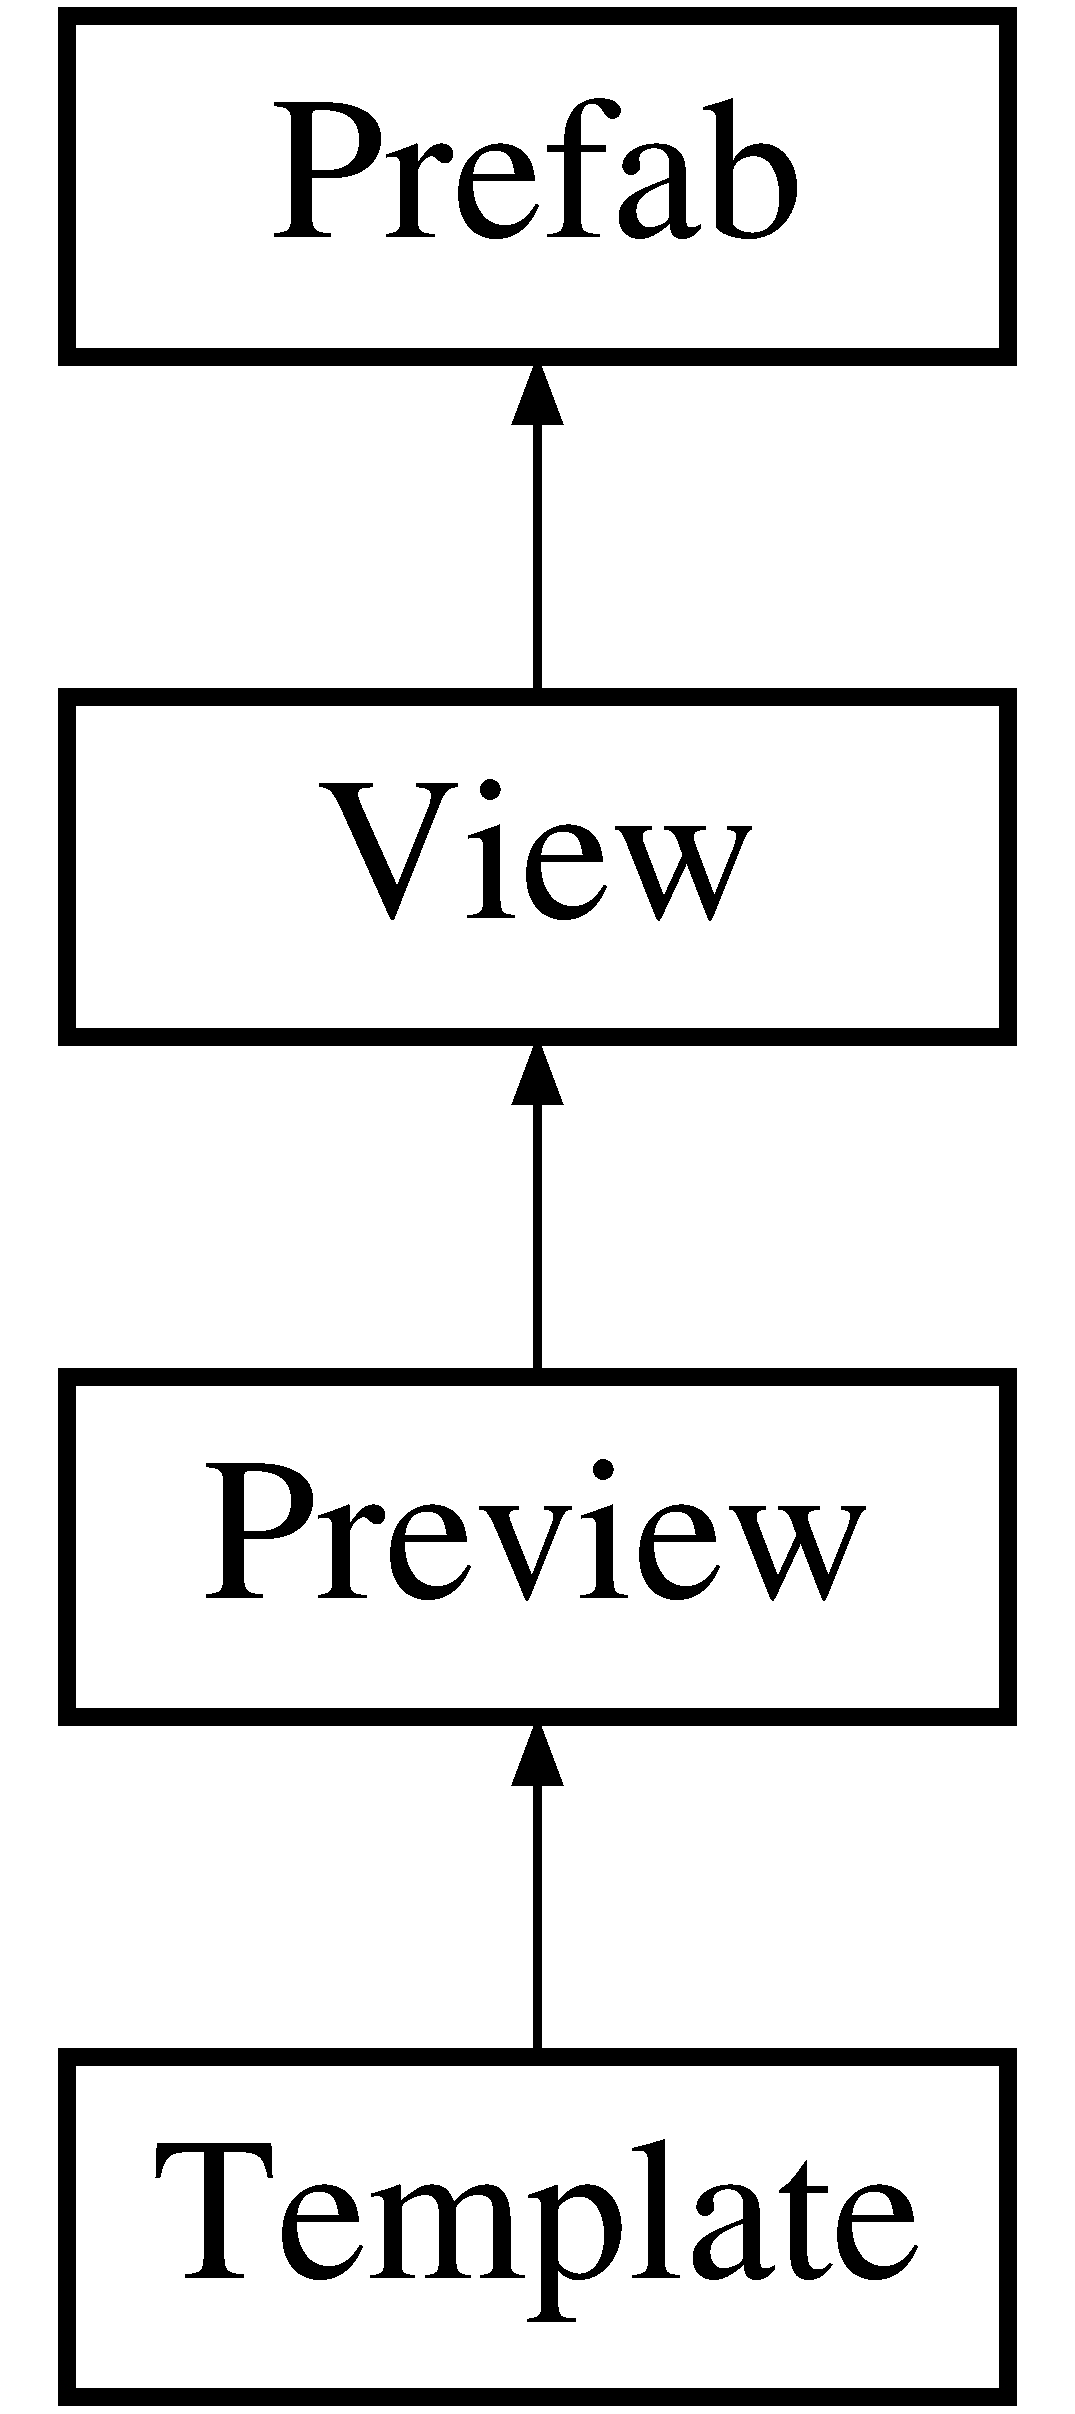
\includegraphics[height=4.000000cm]{class_template}
\end{center}
\end{figure}
\subsection*{Public Member Functions}
\begin{DoxyCompactItemize}
\item 
\hyperlink{class_template_a0e9d773ad8306b0d66337606414a443d}{build} (\$node)
\item 
\hyperlink{class_template_a441602e9d8e2305bee53a34a10b9fa64}{extend} (\$tag, \$func)
\item 
\hyperlink{class_template_a975d2c46a134129eb727fadcadf48adf}{\+\_\+\+\_\+call} (\$func, array \$args)
\item 
\hyperlink{class_template_aad1c85bef0735e4888d8f8e26652f9f7}{parse} (\$text)
\item 
\hyperlink{class_template_a095c5d389db211932136b53f25f39685}{\+\_\+\+\_\+construct} ()
\end{DoxyCompactItemize}
\subsection*{Data Fields}
\begin{DoxyCompactItemize}
\item 
\hypertarget{class_template_aed067c1c25c780570d3191ee878d0ba2}{}\label{class_template_aed067c1c25c780570d3191ee878d0ba2} 
\hyperlink{class_template_aed067c1c25c780570d3191ee878d0ba2}{\$custom} =\mbox{[}$\,$\mbox{]}
\begin{DoxyCompactList}\small\item\em Custom tag handlers. \end{DoxyCompactList}\end{DoxyCompactItemize}
{\bf }\par
\begin{DoxyCompactItemize}
\item 
\hypertarget{class_template_a095176974668a9554e3e88442ba21baa}{}\label{class_template_a095176974668a9554e3e88442ba21baa} 
const {\bfseries E\+\_\+\+Method} =\textquotesingle{}Call to undefined method \%s()\textquotesingle{}
\end{DoxyCompactItemize}

\subsection*{Protected Member Functions}
\begin{DoxyCompactItemize}
\item 
\hyperlink{class_template_a38478c9981f9204a5f7a8ebe9c2e0f1f}{\+\_\+set} (array \$node)
\item 
\hyperlink{class_template_a93c6aa31effa27eea4ab693d6ee6bc56}{\+\_\+include} (array \$node)
\item 
\hyperlink{class_template_af5abab1b9b7dd5911927de68b50b74da}{\+\_\+exclude} ()
\item 
\hyperlink{class_template_a8e0acee0de043ee22d704799c0858dda}{\+\_\+ignore} (array \$node)
\item 
\hyperlink{class_template_acd0e2435a35935eb2c0b6f7d5593b11a}{\+\_\+loop} (array \$node)
\item 
\hyperlink{class_template_a39819dbd44517f7266ef5e39bcc37751}{\+\_\+repeat} (array \$node)
\item 
\hyperlink{class_template_a3a731dbfb5232fd26198927fcd60c886}{\+\_\+check} (array \$node)
\item 
\hyperlink{class_template_a6ec27da12c49157c7cf38f3a68a3890d}{\+\_\+true} (array \$node)
\item 
\hyperlink{class_template_ae21eec23514830fab4659fff6d031fac}{\+\_\+false} (array \$node)
\item 
\hyperlink{class_template_a2d73ae3b02526a59f54115681884da3a}{\+\_\+switch} (array \$node)
\item 
\hyperlink{class_template_ae79c95442d3831174486776ca3090bb6}{\+\_\+case} (array \$node)
\item 
\hyperlink{class_template_a3d2700d4b385c03361417f50f13e8985}{\+\_\+default} (array \$node)
\end{DoxyCompactItemize}
\subsection*{Protected Attributes}
\begin{DoxyCompactItemize}
\item 
\hypertarget{class_template_a475a6a63b85186663d34151bcbd21590}{}\label{class_template_a475a6a63b85186663d34151bcbd21590} 
\hyperlink{class_template_a475a6a63b85186663d34151bcbd21590}{\$tags}
\begin{DoxyCompactList}\small\item\em \hyperlink{class_template}{Template} tags. \end{DoxyCompactList}\end{DoxyCompactItemize}
\subsection*{Additional Inherited Members}


\subsection{Detailed Description}
X\+M\+L-\/style template engine. 

Definition at line 24 of file template.\+php.



\subsection{Constructor \& Destructor Documentation}
\hypertarget{class_template_a095c5d389db211932136b53f25f39685}{}\label{class_template_a095c5d389db211932136b53f25f39685} 
\index{Template@{Template}!\+\_\+\+\_\+construct@{\+\_\+\+\_\+construct}}
\index{\+\_\+\+\_\+construct@{\+\_\+\+\_\+construct}!Template@{Template}}
\subsubsection{\texorpdfstring{\+\_\+\+\_\+construct()}{\_\_construct()}}
{\footnotesize\ttfamily \+\_\+\+\_\+construct (\begin{DoxyParamCaption}{ }\end{DoxyParamCaption})}

Class constructor return object 

Definition at line 341 of file template.\+php.



\subsection{Member Function Documentation}
\hypertarget{class_template_a975d2c46a134129eb727fadcadf48adf}{}\label{class_template_a975d2c46a134129eb727fadcadf48adf} 
\index{Template@{Template}!\+\_\+\+\_\+call@{\+\_\+\+\_\+call}}
\index{\+\_\+\+\_\+call@{\+\_\+\+\_\+call}!Template@{Template}}
\subsubsection{\texorpdfstring{\+\_\+\+\_\+call()}{\_\_call()}}
{\footnotesize\ttfamily \+\_\+\+\_\+call (\begin{DoxyParamCaption}\item[{}]{\$func,  }\item[{array}]{\$args }\end{DoxyParamCaption})}

Call custom tag handler \begin{DoxyReturn}{Returns}
string$\vert$\+F\+A\+L\+SE 
\end{DoxyReturn}

\begin{DoxyParams}{Parameters}
{\em \$func} & callback \\
\hline
{\em \$args} & array \\
\hline
\end{DoxyParams}


Definition at line 258 of file template.\+php.

\hypertarget{class_template_ae79c95442d3831174486776ca3090bb6}{}\label{class_template_ae79c95442d3831174486776ca3090bb6} 
\index{Template@{Template}!\+\_\+case@{\+\_\+case}}
\index{\+\_\+case@{\+\_\+case}!Template@{Template}}
\subsubsection{\texorpdfstring{\+\_\+case()}{\_case()}}
{\footnotesize\ttfamily \+\_\+case (\begin{DoxyParamCaption}\item[{array}]{\$node }\end{DoxyParamCaption})\hspace{0.3cm}{\ttfamily [protected]}}

\hyperlink{class_template}{Template} -\/case-\/ tag handler \begin{DoxyReturn}{Returns}
string 
\end{DoxyReturn}

\begin{DoxyParams}{Parameters}
{\em \$node} & array \\
\hline
\end{DoxyParams}


Definition at line 202 of file template.\+php.

\hypertarget{class_template_a3a731dbfb5232fd26198927fcd60c886}{}\label{class_template_a3a731dbfb5232fd26198927fcd60c886} 
\index{Template@{Template}!\+\_\+check@{\+\_\+check}}
\index{\+\_\+check@{\+\_\+check}!Template@{Template}}
\subsubsection{\texorpdfstring{\+\_\+check()}{\_check()}}
{\footnotesize\ttfamily \+\_\+check (\begin{DoxyParamCaption}\item[{array}]{\$node }\end{DoxyParamCaption})\hspace{0.3cm}{\ttfamily [protected]}}

\hyperlink{class_template}{Template} -\/check-\/ tag handler \begin{DoxyReturn}{Returns}
string 
\end{DoxyReturn}

\begin{DoxyParams}{Parameters}
{\em \$node} & array \\
\hline
\end{DoxyParams}


Definition at line 144 of file template.\+php.

\hypertarget{class_template_a3d2700d4b385c03361417f50f13e8985}{}\label{class_template_a3d2700d4b385c03361417f50f13e8985} 
\index{Template@{Template}!\+\_\+default@{\+\_\+default}}
\index{\+\_\+default@{\+\_\+default}!Template@{Template}}
\subsubsection{\texorpdfstring{\+\_\+default()}{\_default()}}
{\footnotesize\ttfamily \+\_\+default (\begin{DoxyParamCaption}\item[{array}]{\$node }\end{DoxyParamCaption})\hspace{0.3cm}{\ttfamily [protected]}}

\hyperlink{class_template}{Template} -\/default-\/ tag handler \begin{DoxyReturn}{Returns}
string 
\end{DoxyReturn}

\begin{DoxyParams}{Parameters}
{\em \$node} & array \\
\hline
\end{DoxyParams}


Definition at line 220 of file template.\+php.

\hypertarget{class_template_af5abab1b9b7dd5911927de68b50b74da}{}\label{class_template_af5abab1b9b7dd5911927de68b50b74da} 
\index{Template@{Template}!\+\_\+exclude@{\+\_\+exclude}}
\index{\+\_\+exclude@{\+\_\+exclude}!Template@{Template}}
\subsubsection{\texorpdfstring{\+\_\+exclude()}{\_exclude()}}
{\footnotesize\ttfamily \+\_\+exclude (\begin{DoxyParamCaption}{ }\end{DoxyParamCaption})\hspace{0.3cm}{\ttfamily [protected]}}

\hyperlink{class_template}{Template} -\/exclude-\/ tag handler \begin{DoxyReturn}{Returns}
string 
\end{DoxyReturn}


Definition at line 87 of file template.\+php.

\hypertarget{class_template_ae21eec23514830fab4659fff6d031fac}{}\label{class_template_ae21eec23514830fab4659fff6d031fac} 
\index{Template@{Template}!\+\_\+false@{\+\_\+false}}
\index{\+\_\+false@{\+\_\+false}!Template@{Template}}
\subsubsection{\texorpdfstring{\+\_\+false()}{\_false()}}
{\footnotesize\ttfamily \+\_\+false (\begin{DoxyParamCaption}\item[{array}]{\$node }\end{DoxyParamCaption})\hspace{0.3cm}{\ttfamily [protected]}}

\hyperlink{class_template}{Template} -\/false-\/ tag handler \begin{DoxyReturn}{Returns}
string 
\end{DoxyReturn}

\begin{DoxyParams}{Parameters}
{\em \$node} & array \\
\hline
\end{DoxyParams}


Definition at line 176 of file template.\+php.

\hypertarget{class_template_a8e0acee0de043ee22d704799c0858dda}{}\label{class_template_a8e0acee0de043ee22d704799c0858dda} 
\index{Template@{Template}!\+\_\+ignore@{\+\_\+ignore}}
\index{\+\_\+ignore@{\+\_\+ignore}!Template@{Template}}
\subsubsection{\texorpdfstring{\+\_\+ignore()}{\_ignore()}}
{\footnotesize\ttfamily \+\_\+ignore (\begin{DoxyParamCaption}\item[{array}]{\$node }\end{DoxyParamCaption})\hspace{0.3cm}{\ttfamily [protected]}}

\hyperlink{class_template}{Template} -\/ignore-\/ tag handler \begin{DoxyReturn}{Returns}
string 
\end{DoxyReturn}

\begin{DoxyParams}{Parameters}
{\em \$node} & array \\
\hline
\end{DoxyParams}


Definition at line 96 of file template.\+php.

\hypertarget{class_template_a93c6aa31effa27eea4ab693d6ee6bc56}{}\label{class_template_a93c6aa31effa27eea4ab693d6ee6bc56} 
\index{Template@{Template}!\+\_\+include@{\+\_\+include}}
\index{\+\_\+include@{\+\_\+include}!Template@{Template}}
\subsubsection{\texorpdfstring{\+\_\+include()}{\_include()}}
{\footnotesize\ttfamily \+\_\+include (\begin{DoxyParamCaption}\item[{array}]{\$node }\end{DoxyParamCaption})\hspace{0.3cm}{\ttfamily [protected]}}

\hyperlink{class_template}{Template} -\/include-\/ tag handler \begin{DoxyReturn}{Returns}
string 
\end{DoxyReturn}

\begin{DoxyParams}{Parameters}
{\em \$node} & array \\
\hline
\end{DoxyParams}


Definition at line 57 of file template.\+php.

\hypertarget{class_template_acd0e2435a35935eb2c0b6f7d5593b11a}{}\label{class_template_acd0e2435a35935eb2c0b6f7d5593b11a} 
\index{Template@{Template}!\+\_\+loop@{\+\_\+loop}}
\index{\+\_\+loop@{\+\_\+loop}!Template@{Template}}
\subsubsection{\texorpdfstring{\+\_\+loop()}{\_loop()}}
{\footnotesize\ttfamily \+\_\+loop (\begin{DoxyParamCaption}\item[{array}]{\$node }\end{DoxyParamCaption})\hspace{0.3cm}{\ttfamily [protected]}}

\hyperlink{class_template}{Template} -\/loop-\/ tag handler \begin{DoxyReturn}{Returns}
string 
\end{DoxyReturn}

\begin{DoxyParams}{Parameters}
{\em \$node} & array \\
\hline
\end{DoxyParams}


Definition at line 105 of file template.\+php.

\hypertarget{class_template_a39819dbd44517f7266ef5e39bcc37751}{}\label{class_template_a39819dbd44517f7266ef5e39bcc37751} 
\index{Template@{Template}!\+\_\+repeat@{\+\_\+repeat}}
\index{\+\_\+repeat@{\+\_\+repeat}!Template@{Template}}
\subsubsection{\texorpdfstring{\+\_\+repeat()}{\_repeat()}}
{\footnotesize\ttfamily \+\_\+repeat (\begin{DoxyParamCaption}\item[{array}]{\$node }\end{DoxyParamCaption})\hspace{0.3cm}{\ttfamily [protected]}}

\hyperlink{class_template}{Template} -\/repeat-\/ tag handler \begin{DoxyReturn}{Returns}
string 
\end{DoxyReturn}

\begin{DoxyParams}{Parameters}
{\em \$node} & array \\
\hline
\end{DoxyParams}


Definition at line 122 of file template.\+php.

\hypertarget{class_template_a38478c9981f9204a5f7a8ebe9c2e0f1f}{}\label{class_template_a38478c9981f9204a5f7a8ebe9c2e0f1f} 
\index{Template@{Template}!\+\_\+set@{\+\_\+set}}
\index{\+\_\+set@{\+\_\+set}!Template@{Template}}
\subsubsection{\texorpdfstring{\+\_\+set()}{\_set()}}
{\footnotesize\ttfamily \+\_\+set (\begin{DoxyParamCaption}\item[{array}]{\$node }\end{DoxyParamCaption})\hspace{0.3cm}{\ttfamily [protected]}}

\hyperlink{class_template}{Template} -\/set-\/ tag handler \begin{DoxyReturn}{Returns}
string 
\end{DoxyReturn}

\begin{DoxyParams}{Parameters}
{\em \$node} & array \\
\hline
\end{DoxyParams}


Definition at line 42 of file template.\+php.

\hypertarget{class_template_a2d73ae3b02526a59f54115681884da3a}{}\label{class_template_a2d73ae3b02526a59f54115681884da3a} 
\index{Template@{Template}!\+\_\+switch@{\+\_\+switch}}
\index{\+\_\+switch@{\+\_\+switch}!Template@{Template}}
\subsubsection{\texorpdfstring{\+\_\+switch()}{\_switch()}}
{\footnotesize\ttfamily \+\_\+switch (\begin{DoxyParamCaption}\item[{array}]{\$node }\end{DoxyParamCaption})\hspace{0.3cm}{\ttfamily [protected]}}

\hyperlink{class_template}{Template} -\/switch-\/ tag handler \begin{DoxyReturn}{Returns}
string 
\end{DoxyReturn}

\begin{DoxyParams}{Parameters}
{\em \$node} & array \\
\hline
\end{DoxyParams}


Definition at line 185 of file template.\+php.

\hypertarget{class_template_a6ec27da12c49157c7cf38f3a68a3890d}{}\label{class_template_a6ec27da12c49157c7cf38f3a68a3890d} 
\index{Template@{Template}!\+\_\+true@{\+\_\+true}}
\index{\+\_\+true@{\+\_\+true}!Template@{Template}}
\subsubsection{\texorpdfstring{\+\_\+true()}{\_true()}}
{\footnotesize\ttfamily \+\_\+true (\begin{DoxyParamCaption}\item[{array}]{\$node }\end{DoxyParamCaption})\hspace{0.3cm}{\ttfamily [protected]}}

\hyperlink{class_template}{Template} -\/true-\/ tag handler \begin{DoxyReturn}{Returns}
string 
\end{DoxyReturn}

\begin{DoxyParams}{Parameters}
{\em \$node} & array \\
\hline
\end{DoxyParams}


Definition at line 167 of file template.\+php.

\hypertarget{class_template_a0e9d773ad8306b0d66337606414a443d}{}\label{class_template_a0e9d773ad8306b0d66337606414a443d} 
\index{Template@{Template}!build@{build}}
\index{build@{build}!Template@{Template}}
\subsubsection{\texorpdfstring{build()}{build()}}
{\footnotesize\ttfamily build (\begin{DoxyParamCaption}\item[{}]{\$node }\end{DoxyParamCaption})}

Assemble markup \begin{DoxyReturn}{Returns}
string 
\end{DoxyReturn}

\begin{DoxyParams}{Parameters}
{\em \$node} & array$\vert$string \\
\hline
\end{DoxyParams}


Definition at line 232 of file template.\+php.

\hypertarget{class_template_a441602e9d8e2305bee53a34a10b9fa64}{}\label{class_template_a441602e9d8e2305bee53a34a10b9fa64} 
\index{Template@{Template}!extend@{extend}}
\index{extend@{extend}!Template@{Template}}
\subsubsection{\texorpdfstring{extend()}{extend()}}
{\footnotesize\ttfamily extend (\begin{DoxyParamCaption}\item[{}]{\$tag,  }\item[{}]{\$func }\end{DoxyParamCaption})}

Extend template with custom tag \begin{DoxyReturn}{Returns}
N\+U\+LL 
\end{DoxyReturn}

\begin{DoxyParams}{Parameters}
{\em \$tag} & string \\
\hline
{\em \$func} & callback \\
\hline
\end{DoxyParams}


Definition at line 247 of file template.\+php.

\hypertarget{class_template_aad1c85bef0735e4888d8f8e26652f9f7}{}\label{class_template_aad1c85bef0735e4888d8f8e26652f9f7} 
\index{Template@{Template}!parse@{parse}}
\index{parse@{parse}!Template@{Template}}
\subsubsection{\texorpdfstring{parse()}{parse()}}
{\footnotesize\ttfamily parse (\begin{DoxyParamCaption}\item[{}]{\$text }\end{DoxyParamCaption})}

Parse string for template directives and tokens \begin{DoxyReturn}{Returns}
string$\vert$array 
\end{DoxyReturn}

\begin{DoxyParams}{Parameters}
{\em \$text} & string \\
\hline
\end{DoxyParams}


Definition at line 271 of file template.\+php.



The documentation for this class was generated from the following file\+:\begin{DoxyCompactItemize}
\item 
/\+Users/aplennevaux/\+G\+I\+T\+H\+U\+B/\+Visionary-\/website/src/vendor/bcosca/fatfree/lib/template.\+php\end{DoxyCompactItemize}

\hypertarget{class_test}{}\section{Test Class Reference}
\label{class_test}\index{Test@{Test}}


Unit test kit.  


\subsection*{Public Member Functions}
\begin{DoxyCompactItemize}
\item 
\hyperlink{class_test_a81532ad36ede4bfc6cd5e69a321f3df4}{results} ()
\item 
\hyperlink{class_test_a846b7d46e6d54e369e91f13b8326ec50}{passed} ()
\item 
\hyperlink{class_test_a82ce39187ec69f28ce3ad0b971858c32}{expect} (\$cond, \$text=N\+U\+LL)
\item 
\hyperlink{class_test_a6d386dc62867e5f7426c28c22ca913c6}{message} (\$text)
\item 
\hyperlink{class_test_a54d3be59961cf484bfd4cb83ddabab74}{\+\_\+\+\_\+construct} (\$level=self\+::\+F\+L\+A\+G\+\_\+\+Both)
\end{DoxyCompactItemize}
\subsection*{Data Fields}
\begin{DoxyCompactItemize}
\item 
\hypertarget{class_test_a36f815b75b2e9a2b312e4c61daf87e9a}{}\label{class_test_a36f815b75b2e9a2b312e4c61daf87e9a} 
\hyperlink{class_test_a36f815b75b2e9a2b312e4c61daf87e9a}{\$passed} =T\+R\+UE
\begin{DoxyCompactList}\small\item\em Success indicator. \end{DoxyCompactList}\end{DoxyCompactItemize}
{\bf }\par
\begin{DoxyCompactItemize}
\item 
\hypertarget{class_test_a622dd069e85c588302b34a8f74b67f62}{}\label{class_test_a622dd069e85c588302b34a8f74b67f62} 
const {\bfseries F\+L\+A\+G\+\_\+\+False} =0
\item 
\hypertarget{class_test_a97e6e2fe98188272b4bff029c2c60964}{}\label{class_test_a97e6e2fe98188272b4bff029c2c60964} 
const {\bfseries F\+L\+A\+G\+\_\+\+True} =1
\item 
\hypertarget{class_test_a0639e68a4d3583d8257f2794dcdc259f}{}\label{class_test_a0639e68a4d3583d8257f2794dcdc259f} 
const {\bfseries F\+L\+A\+G\+\_\+\+Both} =2
\end{DoxyCompactItemize}

\subsection*{Protected Attributes}
\begin{DoxyCompactItemize}
\item 
\hypertarget{class_test_a6efc15b5a2314dd4b5aaa556a375c6d6}{}\label{class_test_a6efc15b5a2314dd4b5aaa556a375c6d6} 
\hyperlink{class_test_a6efc15b5a2314dd4b5aaa556a375c6d6}{\$data} =\mbox{[}$\,$\mbox{]}
\begin{DoxyCompactList}\small\item\em \hyperlink{class_test}{Test} results. \end{DoxyCompactList}\end{DoxyCompactItemize}


\subsection{Detailed Description}
Unit test kit. 

Definition at line 24 of file test.\+php.



\subsection{Constructor \& Destructor Documentation}
\hypertarget{class_test_a54d3be59961cf484bfd4cb83ddabab74}{}\label{class_test_a54d3be59961cf484bfd4cb83ddabab74} 
\index{Test@{Test}!\+\_\+\+\_\+construct@{\+\_\+\+\_\+construct}}
\index{\+\_\+\+\_\+construct@{\+\_\+\+\_\+construct}!Test@{Test}}
\subsubsection{\texorpdfstring{\+\_\+\+\_\+construct()}{\_\_construct()}}
{\footnotesize\ttfamily \+\_\+\+\_\+construct (\begin{DoxyParamCaption}\item[{}]{\$level = {\ttfamily self\+:\+:FLAG\+\_\+Both} }\end{DoxyParamCaption})}

Class constructor \begin{DoxyReturn}{Returns}
N\+U\+LL 
\end{DoxyReturn}

\begin{DoxyParams}{Parameters}
{\em \$level} & int \\
\hline
\end{DoxyParams}


Definition at line 92 of file test.\+php.



\subsection{Member Function Documentation}
\hypertarget{class_test_a82ce39187ec69f28ce3ad0b971858c32}{}\label{class_test_a82ce39187ec69f28ce3ad0b971858c32} 
\index{Test@{Test}!expect@{expect}}
\index{expect@{expect}!Test@{Test}}
\subsubsection{\texorpdfstring{expect()}{expect()}}
{\footnotesize\ttfamily expect (\begin{DoxyParamCaption}\item[{}]{\$cond,  }\item[{}]{\$text = {\ttfamily NULL} }\end{DoxyParamCaption})}

Evaluate condition and save test result \begin{DoxyReturn}{Returns}
object 
\end{DoxyReturn}

\begin{DoxyParams}{Parameters}
{\em \$cond} & bool \\
\hline
{\em \$text} & string \\
\hline
\end{DoxyParams}


Definition at line 61 of file test.\+php.

\hypertarget{class_test_a6d386dc62867e5f7426c28c22ca913c6}{}\label{class_test_a6d386dc62867e5f7426c28c22ca913c6} 
\index{Test@{Test}!message@{message}}
\index{message@{message}!Test@{Test}}
\subsubsection{\texorpdfstring{message()}{message()}}
{\footnotesize\ttfamily message (\begin{DoxyParamCaption}\item[{}]{\$text }\end{DoxyParamCaption})}

Append message to test results \begin{DoxyReturn}{Returns}
N\+U\+LL 
\end{DoxyReturn}

\begin{DoxyParams}{Parameters}
{\em \$text} & string \\
\hline
\end{DoxyParams}


Definition at line 83 of file test.\+php.

\hypertarget{class_test_a846b7d46e6d54e369e91f13b8326ec50}{}\label{class_test_a846b7d46e6d54e369e91f13b8326ec50} 
\index{Test@{Test}!passed@{passed}}
\index{passed@{passed}!Test@{Test}}
\subsubsection{\texorpdfstring{passed()}{passed()}}
{\footnotesize\ttfamily passed (\begin{DoxyParamCaption}{ }\end{DoxyParamCaption})}

Return F\+A\+L\+SE if at least one test case fails \begin{DoxyReturn}{Returns}
bool 
\end{DoxyReturn}


Definition at line 51 of file test.\+php.

\hypertarget{class_test_a81532ad36ede4bfc6cd5e69a321f3df4}{}\label{class_test_a81532ad36ede4bfc6cd5e69a321f3df4} 
\index{Test@{Test}!results@{results}}
\index{results@{results}!Test@{Test}}
\subsubsection{\texorpdfstring{results()}{results()}}
{\footnotesize\ttfamily results (\begin{DoxyParamCaption}{ }\end{DoxyParamCaption})}

Return test results \begin{DoxyReturn}{Returns}
array 
\end{DoxyReturn}


Definition at line 43 of file test.\+php.



The documentation for this class was generated from the following file\+:\begin{DoxyCompactItemize}
\item 
/\+Users/aplennevaux/\+G\+I\+T\+H\+U\+B/\+Visionary-\/website/src/vendor/bcosca/fatfree/lib/test.\+php\end{DoxyCompactItemize}

\hypertarget{class_u_t_f}{}\section{U\+TF Class Reference}
\label{class_u_t_f}\index{U\+TF@{U\+TF}}


Unicode string manager.  


Inheritance diagram for U\+TF\+:\begin{figure}[H]
\begin{center}
\leavevmode
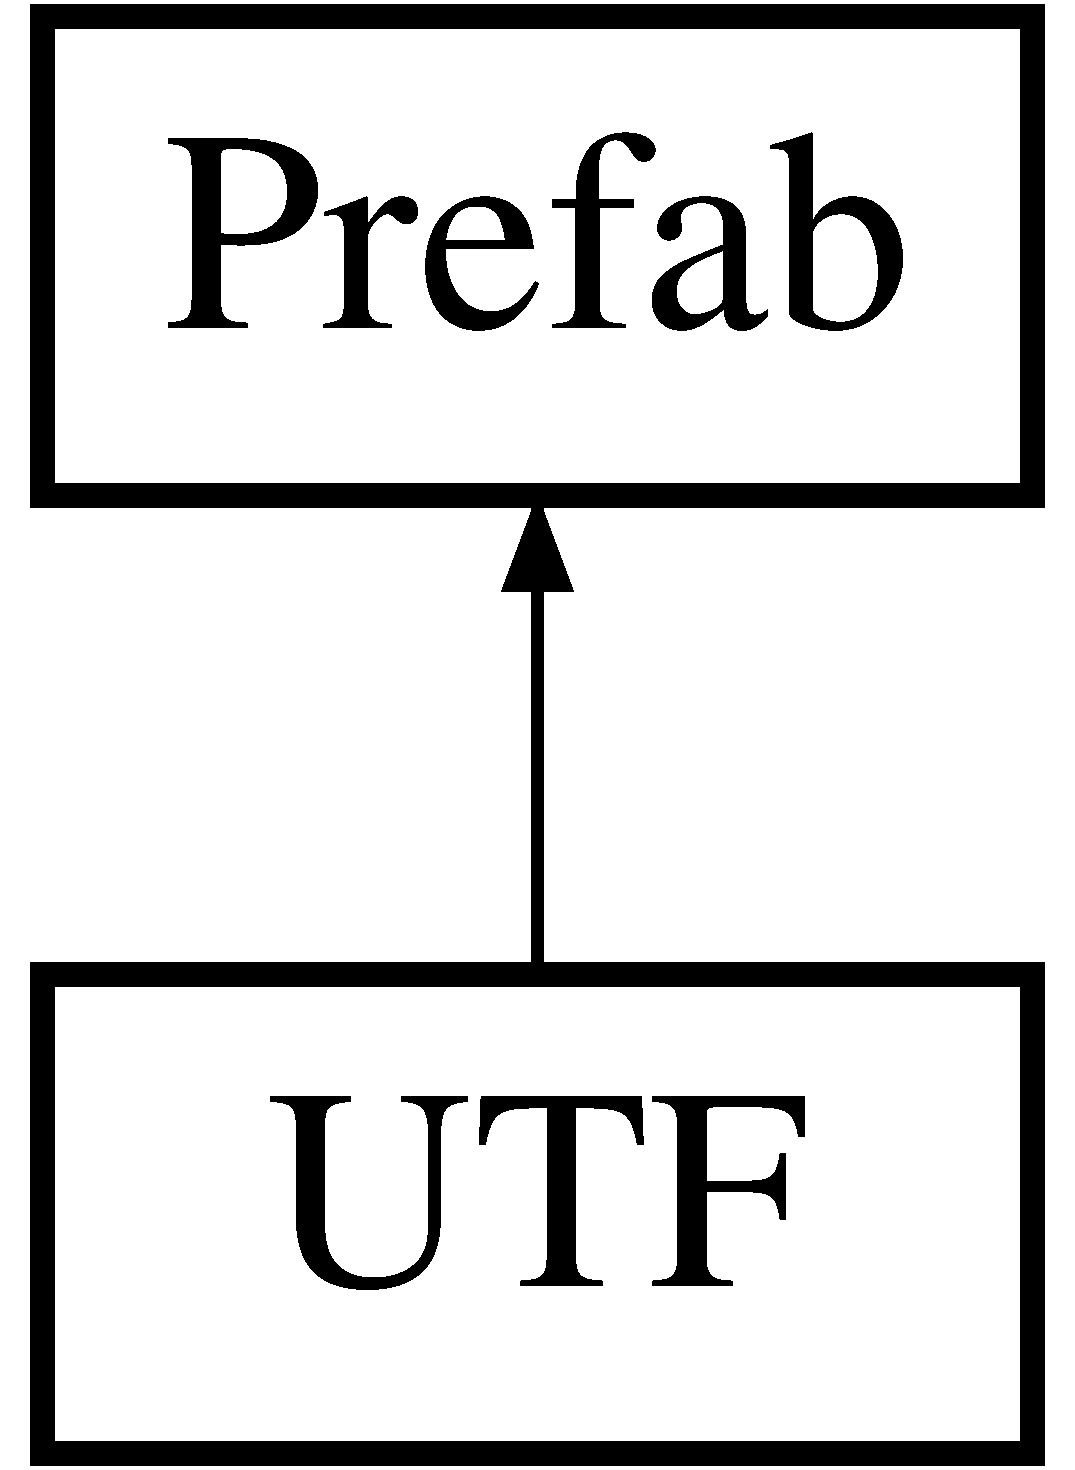
\includegraphics[height=2.000000cm]{class_u_t_f}
\end{center}
\end{figure}
\subsection*{Public Member Functions}
\begin{DoxyCompactItemize}
\item 
\hyperlink{class_u_t_f_a6379e4105bda35d62738418b43d6c214}{strlen} (\$str)
\item 
\hyperlink{class_u_t_f_aee5290955ede3ffc95e03032792d6cef}{strrev} (\$str)
\item 
\hyperlink{class_u_t_f_a091781748220e04bdfb81119c2d215ab}{stripos} (\$stack, \$needle, \$ofs=0)
\item 
\hyperlink{class_u_t_f_a3ac4e2d27df237cef0d1d7f5b5858841}{strpos} (\$stack, \$needle, \$ofs=0, \$case=F\+A\+L\+SE)
\item 
\hyperlink{class_u_t_f_ae5a935ae0460ac0723be7eb4c677ae4f}{stristr} (\$stack, \$needle, \$before=F\+A\+L\+SE)
\item 
\hyperlink{class_u_t_f_aede414417475770b5dea3c6975c2e3dd}{strstr} (\$stack, \$needle, \$before=F\+A\+L\+SE, \$case=F\+A\+L\+SE)
\item 
\hyperlink{class_u_t_f_ab012fe0920f5e9be4a09e01bfb81b867}{substr} (\$str, \$start, \$len=0)
\item 
\hyperlink{class_u_t_f_a1ed9fae3a0627f5fc1adbafed4adab86}{substr\+\_\+count} (\$stack, \$needle)
\item 
\hyperlink{class_u_t_f_a36a0151237d3480734de64933f769843}{ltrim} (\$str)
\item 
\hyperlink{class_u_t_f_afa81b944f8aed770a266a9884e3e5049}{rtrim} (\$str)
\item 
\hyperlink{class_u_t_f_a432e7b973a6e6bfa55cced21e75ee29e}{trim} (\$str)
\item 
\hyperlink{class_u_t_f_a5cb12f35229a81f7a869171b000573b8}{bom} ()
\item 
\hyperlink{class_u_t_f_a798f9e9997b8a6f34ff111df63531c08}{translate} (\$str)
\item 
\hyperlink{class_u_t_f_aaf95120818560ee5ba86d5f4efba6671}{emojify} (\$str)
\end{DoxyCompactItemize}
\subsection*{Additional Inherited Members}


\subsection{Detailed Description}
Unicode string manager. 

Definition at line 24 of file utf.\+php.



\subsection{Member Function Documentation}
\hypertarget{class_u_t_f_a5cb12f35229a81f7a869171b000573b8}{}\label{class_u_t_f_a5cb12f35229a81f7a869171b000573b8} 
\index{U\+TF@{U\+TF}!bom@{bom}}
\index{bom@{bom}!U\+TF@{U\+TF}}
\subsubsection{\texorpdfstring{bom()}{bom()}}
{\footnotesize\ttfamily bom (\begin{DoxyParamCaption}{ }\end{DoxyParamCaption})}

Return U\+T\+F-\/8 byte order mark \begin{DoxyReturn}{Returns}
string 
\end{DoxyReturn}


Definition at line 163 of file utf.\+php.

\hypertarget{class_u_t_f_aaf95120818560ee5ba86d5f4efba6671}{}\label{class_u_t_f_aaf95120818560ee5ba86d5f4efba6671} 
\index{U\+TF@{U\+TF}!emojify@{emojify}}
\index{emojify@{emojify}!U\+TF@{U\+TF}}
\subsubsection{\texorpdfstring{emojify()}{emojify()}}
{\footnotesize\ttfamily emojify (\begin{DoxyParamCaption}\item[{}]{\$str }\end{DoxyParamCaption})}

Translate emoji tokens to Unicode font-\/supported symbols \begin{DoxyReturn}{Returns}
string 
\end{DoxyReturn}

\begin{DoxyParams}{Parameters}
{\em \$str} & string \\
\hline
\end{DoxyParams}


Definition at line 182 of file utf.\+php.

\hypertarget{class_u_t_f_a36a0151237d3480734de64933f769843}{}\label{class_u_t_f_a36a0151237d3480734de64933f769843} 
\index{U\+TF@{U\+TF}!ltrim@{ltrim}}
\index{ltrim@{ltrim}!U\+TF@{U\+TF}}
\subsubsection{\texorpdfstring{ltrim()}{ltrim()}}
{\footnotesize\ttfamily ltrim (\begin{DoxyParamCaption}\item[{}]{\$str }\end{DoxyParamCaption})}

Strip whitespaces from the beginning of a string \begin{DoxyReturn}{Returns}
string 
\end{DoxyReturn}

\begin{DoxyParams}{Parameters}
{\em \$str} & string \\
\hline
\end{DoxyParams}


Definition at line 137 of file utf.\+php.

\hypertarget{class_u_t_f_afa81b944f8aed770a266a9884e3e5049}{}\label{class_u_t_f_afa81b944f8aed770a266a9884e3e5049} 
\index{U\+TF@{U\+TF}!rtrim@{rtrim}}
\index{rtrim@{rtrim}!U\+TF@{U\+TF}}
\subsubsection{\texorpdfstring{rtrim()}{rtrim()}}
{\footnotesize\ttfamily rtrim (\begin{DoxyParamCaption}\item[{}]{\$str }\end{DoxyParamCaption})}

Strip whitespaces from the end of a string \begin{DoxyReturn}{Returns}
string 
\end{DoxyReturn}

\begin{DoxyParams}{Parameters}
{\em \$str} & string \\
\hline
\end{DoxyParams}


Definition at line 146 of file utf.\+php.

\hypertarget{class_u_t_f_a091781748220e04bdfb81119c2d215ab}{}\label{class_u_t_f_a091781748220e04bdfb81119c2d215ab} 
\index{U\+TF@{U\+TF}!stripos@{stripos}}
\index{stripos@{stripos}!U\+TF@{U\+TF}}
\subsubsection{\texorpdfstring{stripos()}{stripos()}}
{\footnotesize\ttfamily stripos (\begin{DoxyParamCaption}\item[{}]{\$stack,  }\item[{}]{\$needle,  }\item[{}]{\$ofs = {\ttfamily 0} }\end{DoxyParamCaption})}

Find position of first occurrence of a string (case-\/insensitive) \begin{DoxyReturn}{Returns}
int$\vert$\+F\+A\+L\+SE 
\end{DoxyReturn}

\begin{DoxyParams}{Parameters}
{\em \$stack} & string \\
\hline
{\em \$needle} & string \\
\hline
{\em \$ofs} & int \\
\hline
\end{DoxyParams}


Definition at line 53 of file utf.\+php.

\hypertarget{class_u_t_f_ae5a935ae0460ac0723be7eb4c677ae4f}{}\label{class_u_t_f_ae5a935ae0460ac0723be7eb4c677ae4f} 
\index{U\+TF@{U\+TF}!stristr@{stristr}}
\index{stristr@{stristr}!U\+TF@{U\+TF}}
\subsubsection{\texorpdfstring{stristr()}{stristr()}}
{\footnotesize\ttfamily stristr (\begin{DoxyParamCaption}\item[{}]{\$stack,  }\item[{}]{\$needle,  }\item[{}]{\$before = {\ttfamily FALSE} }\end{DoxyParamCaption})}

Returns part of haystack string from the first occurrence of needle to the end of haystack (case-\/insensitive) \begin{DoxyReturn}{Returns}
string$\vert$\+F\+A\+L\+SE 
\end{DoxyReturn}

\begin{DoxyParams}{Parameters}
{\em \$stack} & string \\
\hline
{\em \$needle} & string \\
\hline
{\em \$before} & bool \\
\hline
\end{DoxyParams}


Definition at line 79 of file utf.\+php.

\hypertarget{class_u_t_f_a6379e4105bda35d62738418b43d6c214}{}\label{class_u_t_f_a6379e4105bda35d62738418b43d6c214} 
\index{U\+TF@{U\+TF}!strlen@{strlen}}
\index{strlen@{strlen}!U\+TF@{U\+TF}}
\subsubsection{\texorpdfstring{strlen()}{strlen()}}
{\footnotesize\ttfamily strlen (\begin{DoxyParamCaption}\item[{}]{\$str }\end{DoxyParamCaption})}

Get string length \begin{DoxyReturn}{Returns}
int 
\end{DoxyReturn}

\begin{DoxyParams}{Parameters}
{\em \$str} & string \\
\hline
\end{DoxyParams}


Definition at line 31 of file utf.\+php.

\hypertarget{class_u_t_f_a3ac4e2d27df237cef0d1d7f5b5858841}{}\label{class_u_t_f_a3ac4e2d27df237cef0d1d7f5b5858841} 
\index{U\+TF@{U\+TF}!strpos@{strpos}}
\index{strpos@{strpos}!U\+TF@{U\+TF}}
\subsubsection{\texorpdfstring{strpos()}{strpos()}}
{\footnotesize\ttfamily strpos (\begin{DoxyParamCaption}\item[{}]{\$stack,  }\item[{}]{\$needle,  }\item[{}]{\$ofs = {\ttfamily 0},  }\item[{}]{\$case = {\ttfamily FALSE} }\end{DoxyParamCaption})}

Find position of first occurrence of a string \begin{DoxyReturn}{Returns}
int$\vert$\+F\+A\+L\+SE 
\end{DoxyReturn}

\begin{DoxyParams}{Parameters}
{\em \$stack} & string \\
\hline
{\em \$needle} & string \\
\hline
{\em \$ofs} & int \\
\hline
{\em \$case} & bool \\
\hline
\end{DoxyParams}


Definition at line 65 of file utf.\+php.

\hypertarget{class_u_t_f_aee5290955ede3ffc95e03032792d6cef}{}\label{class_u_t_f_aee5290955ede3ffc95e03032792d6cef} 
\index{U\+TF@{U\+TF}!strrev@{strrev}}
\index{strrev@{strrev}!U\+TF@{U\+TF}}
\subsubsection{\texorpdfstring{strrev()}{strrev()}}
{\footnotesize\ttfamily strrev (\begin{DoxyParamCaption}\item[{}]{\$str }\end{DoxyParamCaption})}

Reverse a string \begin{DoxyReturn}{Returns}
string 
\end{DoxyReturn}

\begin{DoxyParams}{Parameters}
{\em \$str} & string \\
\hline
\end{DoxyParams}


Definition at line 41 of file utf.\+php.

\hypertarget{class_u_t_f_aede414417475770b5dea3c6975c2e3dd}{}\label{class_u_t_f_aede414417475770b5dea3c6975c2e3dd} 
\index{U\+TF@{U\+TF}!strstr@{strstr}}
\index{strstr@{strstr}!U\+TF@{U\+TF}}
\subsubsection{\texorpdfstring{strstr()}{strstr()}}
{\footnotesize\ttfamily strstr (\begin{DoxyParamCaption}\item[{}]{\$stack,  }\item[{}]{\$needle,  }\item[{}]{\$before = {\ttfamily FALSE},  }\item[{}]{\$case = {\ttfamily FALSE} }\end{DoxyParamCaption})}

Returns part of haystack string from the first occurrence of needle to the end of haystack \begin{DoxyReturn}{Returns}
string$\vert$\+F\+A\+L\+SE 
\end{DoxyReturn}

\begin{DoxyParams}{Parameters}
{\em \$stack} & string \\
\hline
{\em \$needle} & string \\
\hline
{\em \$before} & bool \\
\hline
{\em \$case} & bool \\
\hline
\end{DoxyParams}


Definition at line 92 of file utf.\+php.

\hypertarget{class_u_t_f_ab012fe0920f5e9be4a09e01bfb81b867}{}\label{class_u_t_f_ab012fe0920f5e9be4a09e01bfb81b867} 
\index{U\+TF@{U\+TF}!substr@{substr}}
\index{substr@{substr}!U\+TF@{U\+TF}}
\subsubsection{\texorpdfstring{substr()}{substr()}}
{\footnotesize\ttfamily substr (\begin{DoxyParamCaption}\item[{}]{\$str,  }\item[{}]{\$start,  }\item[{}]{\$len = {\ttfamily 0} }\end{DoxyParamCaption})}

Return part of a string \begin{DoxyReturn}{Returns}
string$\vert$\+F\+A\+L\+SE 
\end{DoxyReturn}

\begin{DoxyParams}{Parameters}
{\em \$str} & string \\
\hline
{\em \$start} & int \\
\hline
{\em \$len} & int \\
\hline
\end{DoxyParams}


Definition at line 111 of file utf.\+php.

\hypertarget{class_u_t_f_a1ed9fae3a0627f5fc1adbafed4adab86}{}\label{class_u_t_f_a1ed9fae3a0627f5fc1adbafed4adab86} 
\index{U\+TF@{U\+TF}!substr\+\_\+count@{substr\+\_\+count}}
\index{substr\+\_\+count@{substr\+\_\+count}!U\+TF@{U\+TF}}
\subsubsection{\texorpdfstring{substr\+\_\+count()}{substr\_count()}}
{\footnotesize\ttfamily substr\+\_\+count (\begin{DoxyParamCaption}\item[{}]{\$stack,  }\item[{}]{\$needle }\end{DoxyParamCaption})}

Count the number of substring occurrences \begin{DoxyReturn}{Returns}
int 
\end{DoxyReturn}

\begin{DoxyParams}{Parameters}
{\em \$stack} & string \\
\hline
{\em \$needle} & string \\
\hline
\end{DoxyParams}


Definition at line 126 of file utf.\+php.

\hypertarget{class_u_t_f_a798f9e9997b8a6f34ff111df63531c08}{}\label{class_u_t_f_a798f9e9997b8a6f34ff111df63531c08} 
\index{U\+TF@{U\+TF}!translate@{translate}}
\index{translate@{translate}!U\+TF@{U\+TF}}
\subsubsection{\texorpdfstring{translate()}{translate()}}
{\footnotesize\ttfamily translate (\begin{DoxyParamCaption}\item[{}]{\$str }\end{DoxyParamCaption})}

Convert code points to Unicode symbols \begin{DoxyReturn}{Returns}
string 
\end{DoxyReturn}

\begin{DoxyParams}{Parameters}
{\em \$str} & string \\
\hline
\end{DoxyParams}


Definition at line 172 of file utf.\+php.

\hypertarget{class_u_t_f_a432e7b973a6e6bfa55cced21e75ee29e}{}\label{class_u_t_f_a432e7b973a6e6bfa55cced21e75ee29e} 
\index{U\+TF@{U\+TF}!trim@{trim}}
\index{trim@{trim}!U\+TF@{U\+TF}}
\subsubsection{\texorpdfstring{trim()}{trim()}}
{\footnotesize\ttfamily trim (\begin{DoxyParamCaption}\item[{}]{\$str }\end{DoxyParamCaption})}

Strip whitespaces from the beginning and end of a string \begin{DoxyReturn}{Returns}
string 
\end{DoxyReturn}

\begin{DoxyParams}{Parameters}
{\em \$str} & string \\
\hline
\end{DoxyParams}


Definition at line 155 of file utf.\+php.



The documentation for this class was generated from the following file\+:\begin{DoxyCompactItemize}
\item 
/\+Users/aplennevaux/\+G\+I\+T\+H\+U\+B/\+Visionary-\/website/src/vendor/bcosca/fatfree/lib/utf.\+php\end{DoxyCompactItemize}

\hypertarget{class_view}{}\section{View Class Reference}
\label{class_view}\index{View@{View}}


\hyperlink{class_view}{View} handler.  


Inheritance diagram for View\+:\begin{figure}[H]
\begin{center}
\leavevmode
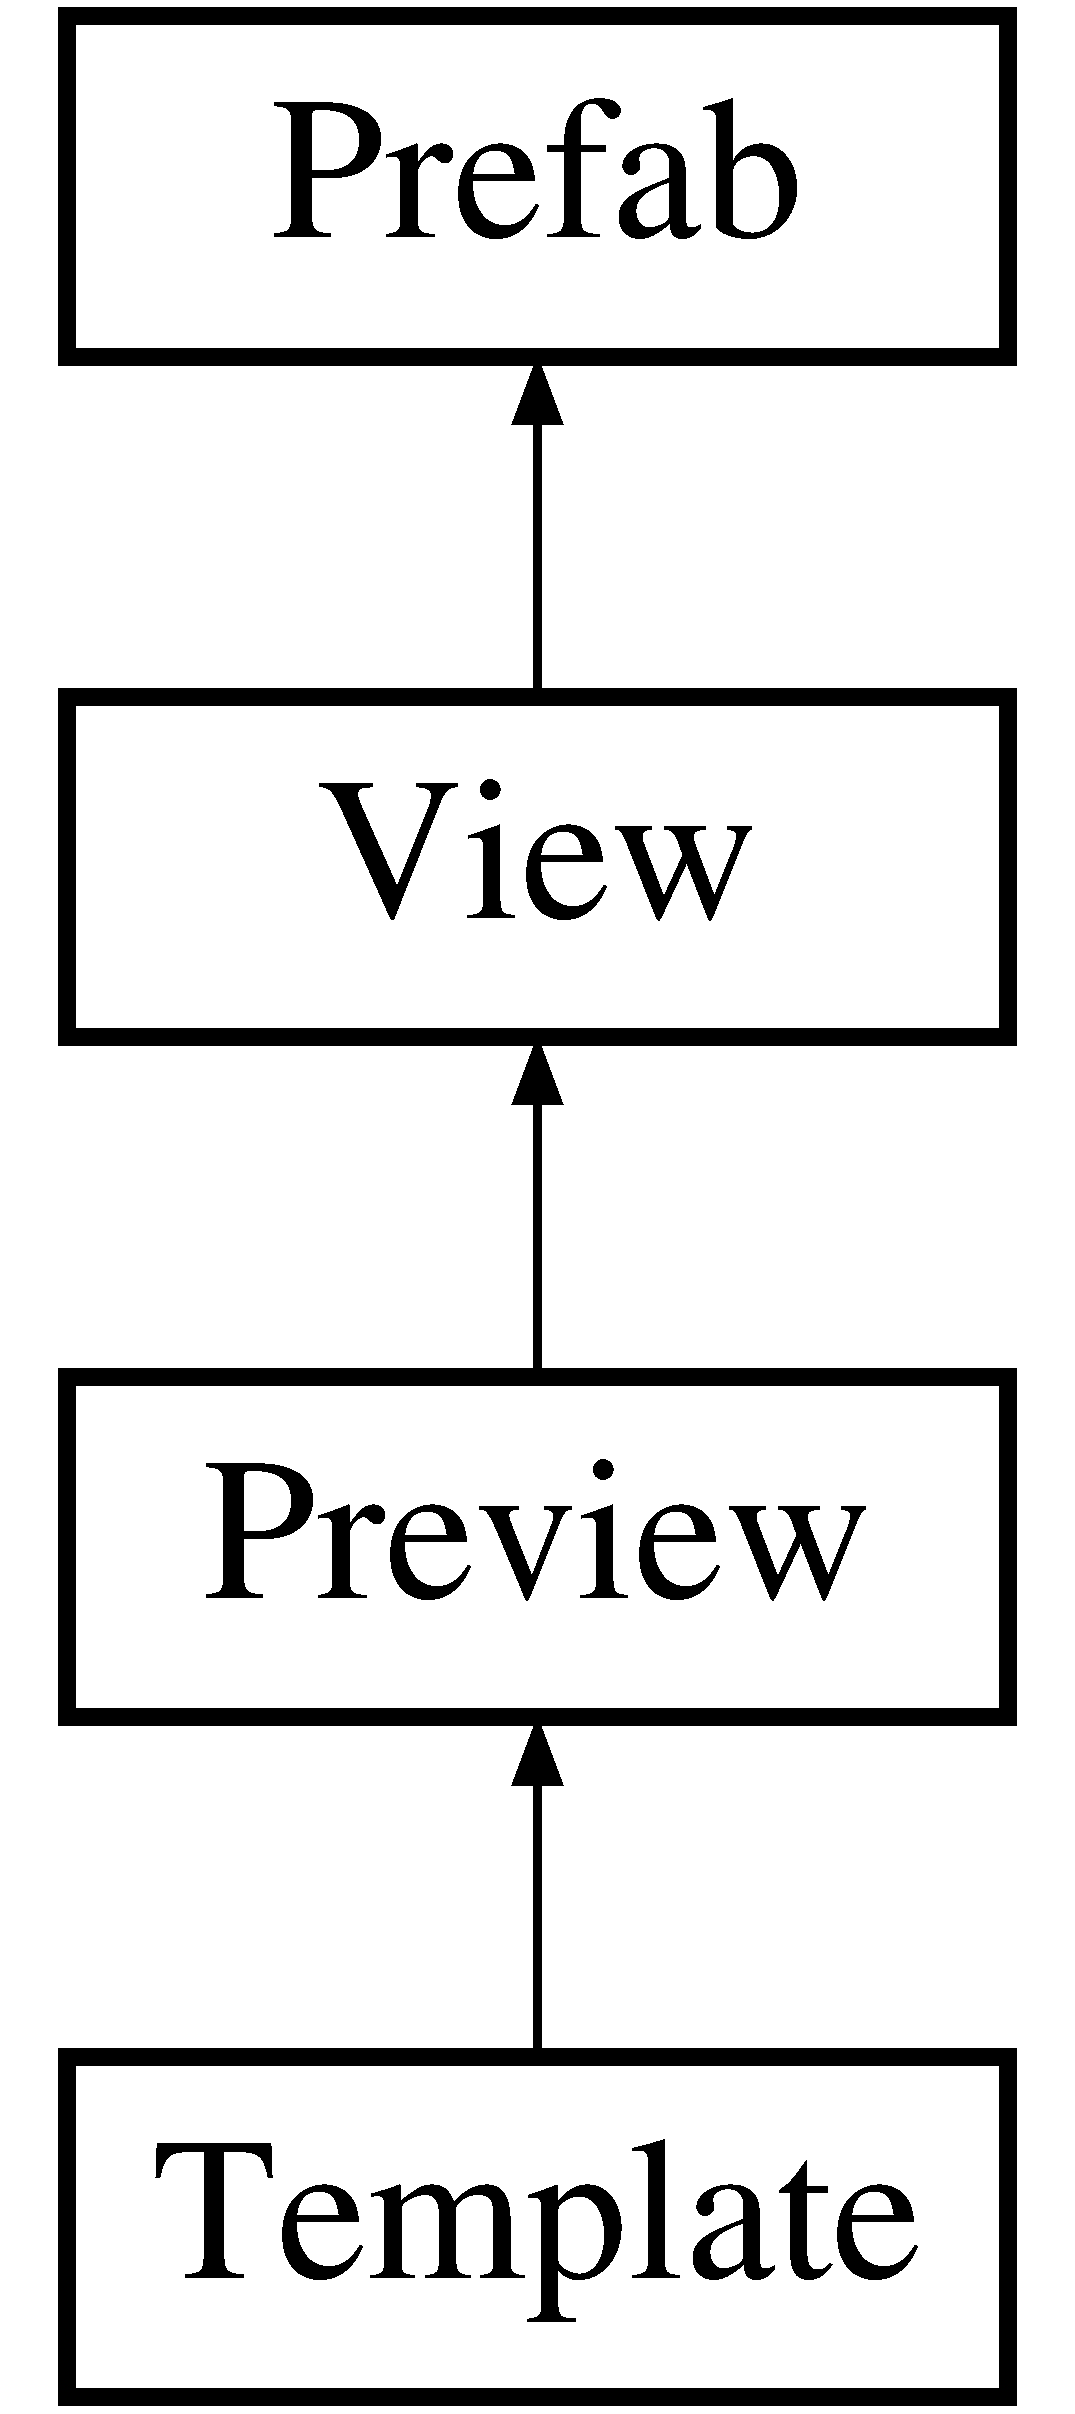
\includegraphics[height=4.000000cm]{class_view}
\end{center}
\end{figure}
\subsection*{Public Member Functions}
\begin{DoxyCompactItemize}
\item 
\hyperlink{class_view_a5bd4df9fdd31ef4ff4e020a04245a34b}{esc} (\$arg)
\item 
\hyperlink{class_view_ae28ae43a12ee2a48b262f167ec9042da}{raw} (\$arg)
\item 
\hyperlink{class_view_a23250d5899cf83753ce12eb47b41ecfb}{render} (\$file, \$mime=\textquotesingle{}text/html\textquotesingle{}, array \$hive=N\+U\+LL, \$ttl=0)
\item 
\hyperlink{class_view_a26528971a7a6dec321d8c96fc4e28d58}{afterrender} (\$func)
\end{DoxyCompactItemize}
\subsection*{Data Fields}
\begin{DoxyCompactItemize}
\item 
\hypertarget{class_view_ae4c540bb943eedf48dbc7d06b2994a05}{}\label{class_view_ae4c540bb943eedf48dbc7d06b2994a05} 
\hyperlink{class_view_ae4c540bb943eedf48dbc7d06b2994a05}{\$trigger}
\begin{DoxyCompactList}\small\item\em post-\/rendering handler \end{DoxyCompactList}\item 
\hypertarget{class_view_abd32cc82c6a3f79491987de36ad580ca}{}\label{class_view_abd32cc82c6a3f79491987de36ad580ca} 
\hyperlink{class_view_abd32cc82c6a3f79491987de36ad580ca}{\$level} =0
\begin{DoxyCompactList}\small\item\em Nesting level. \end{DoxyCompactList}\end{DoxyCompactItemize}
\subsection*{Protected Member Functions}
\begin{DoxyCompactItemize}
\item 
\hyperlink{class_view_a2aae93402f5ee934a00733cc2bd9286a}{sandbox} (array \$hive=N\+U\+LL)
\end{DoxyCompactItemize}
\subsection*{Protected Attributes}
\begin{DoxyCompactItemize}
\item 
\hypertarget{class_view_acccf2eac8663e0cebe8101e90fbab089}{}\label{class_view_acccf2eac8663e0cebe8101e90fbab089} 
\hyperlink{class_view_acccf2eac8663e0cebe8101e90fbab089}{\$view}
\begin{DoxyCompactList}\small\item\em \hyperlink{class_template}{Template} file. \end{DoxyCompactList}\end{DoxyCompactItemize}
\subsection*{Additional Inherited Members}


\subsection{Detailed Description}
\hyperlink{class_view}{View} handler. 

Definition at line 2596 of file base.\+php.



\subsection{Member Function Documentation}
\hypertarget{class_view_a26528971a7a6dec321d8c96fc4e28d58}{}\label{class_view_a26528971a7a6dec321d8c96fc4e28d58} 
\index{View@{View}!afterrender@{afterrender}}
\index{afterrender@{afterrender}!View@{View}}
\subsubsection{\texorpdfstring{afterrender()}{afterrender()}}
{\footnotesize\ttfamily afterrender (\begin{DoxyParamCaption}\item[{}]{\$func }\end{DoxyParamCaption})}

post rendering handler 
\begin{DoxyParams}{Parameters}
{\em \$func} & callback \\
\hline
\end{DoxyParams}


Definition at line 2699 of file base.\+php.

\hypertarget{class_view_a5bd4df9fdd31ef4ff4e020a04245a34b}{}\label{class_view_a5bd4df9fdd31ef4ff4e020a04245a34b} 
\index{View@{View}!esc@{esc}}
\index{esc@{esc}!View@{View}}
\subsubsection{\texorpdfstring{esc()}{esc()}}
{\footnotesize\ttfamily esc (\begin{DoxyParamCaption}\item[{}]{\$arg }\end{DoxyParamCaption})}

Encode characters to equivalent H\+T\+ML entities \begin{DoxyReturn}{Returns}
string 
\end{DoxyReturn}

\begin{DoxyParams}{Parameters}
{\em \$arg} & mixed \\
\hline
\end{DoxyParams}


Definition at line 2611 of file base.\+php.

\hypertarget{class_view_ae28ae43a12ee2a48b262f167ec9042da}{}\label{class_view_ae28ae43a12ee2a48b262f167ec9042da} 
\index{View@{View}!raw@{raw}}
\index{raw@{raw}!View@{View}}
\subsubsection{\texorpdfstring{raw()}{raw()}}
{\footnotesize\ttfamily raw (\begin{DoxyParamCaption}\item[{}]{\$arg }\end{DoxyParamCaption})}

Decode H\+T\+ML entities to equivalent characters \begin{DoxyReturn}{Returns}
string 
\end{DoxyReturn}

\begin{DoxyParams}{Parameters}
{\em \$arg} & mixed \\
\hline
\end{DoxyParams}


Definition at line 2625 of file base.\+php.

\hypertarget{class_view_a23250d5899cf83753ce12eb47b41ecfb}{}\label{class_view_a23250d5899cf83753ce12eb47b41ecfb} 
\index{View@{View}!render@{render}}
\index{render@{render}!View@{View}}
\subsubsection{\texorpdfstring{render()}{render()}}
{\footnotesize\ttfamily render (\begin{DoxyParamCaption}\item[{}]{\$file,  }\item[{}]{\$mime = {\ttfamily \textquotesingle{}text/html\textquotesingle{}},  }\item[{array}]{\$hive = {\ttfamily NULL},  }\item[{}]{\$ttl = {\ttfamily 0} }\end{DoxyParamCaption})}

Render template \begin{DoxyReturn}{Returns}
string 
\end{DoxyReturn}

\begin{DoxyParams}{Parameters}
{\em \$file} & string \\
\hline
{\em \$mime} & string \\
\hline
{\em \$hive} & array \\
\hline
{\em \$ttl} & int \\
\hline
\end{DoxyParams}


Definition at line 2670 of file base.\+php.

\hypertarget{class_view_a2aae93402f5ee934a00733cc2bd9286a}{}\label{class_view_a2aae93402f5ee934a00733cc2bd9286a} 
\index{View@{View}!sandbox@{sandbox}}
\index{sandbox@{sandbox}!View@{View}}
\subsubsection{\texorpdfstring{sandbox()}{sandbox()}}
{\footnotesize\ttfamily sandbox (\begin{DoxyParamCaption}\item[{array}]{\$hive = {\ttfamily NULL} }\end{DoxyParamCaption})\hspace{0.3cm}{\ttfamily [protected]}}

Create sandbox for template execution \begin{DoxyReturn}{Returns}
string 
\end{DoxyReturn}

\begin{DoxyParams}{Parameters}
{\em \$hive} & array \\
\hline
\end{DoxyParams}


Definition at line 2639 of file base.\+php.



The documentation for this class was generated from the following file\+:\begin{DoxyCompactItemize}
\item 
/\+Users/aplennevaux/\+G\+I\+T\+H\+U\+B/\+Visionary-\/website/src/vendor/bcosca/fatfree/lib/base.\+php\end{DoxyCompactItemize}

\hypertarget{class_web}{}\section{Web Class Reference}
\label{class_web}\index{Web@{Web}}


Wrapper for various H\+T\+TP utilities.  


Inheritance diagram for Web\+:\begin{figure}[H]
\begin{center}
\leavevmode
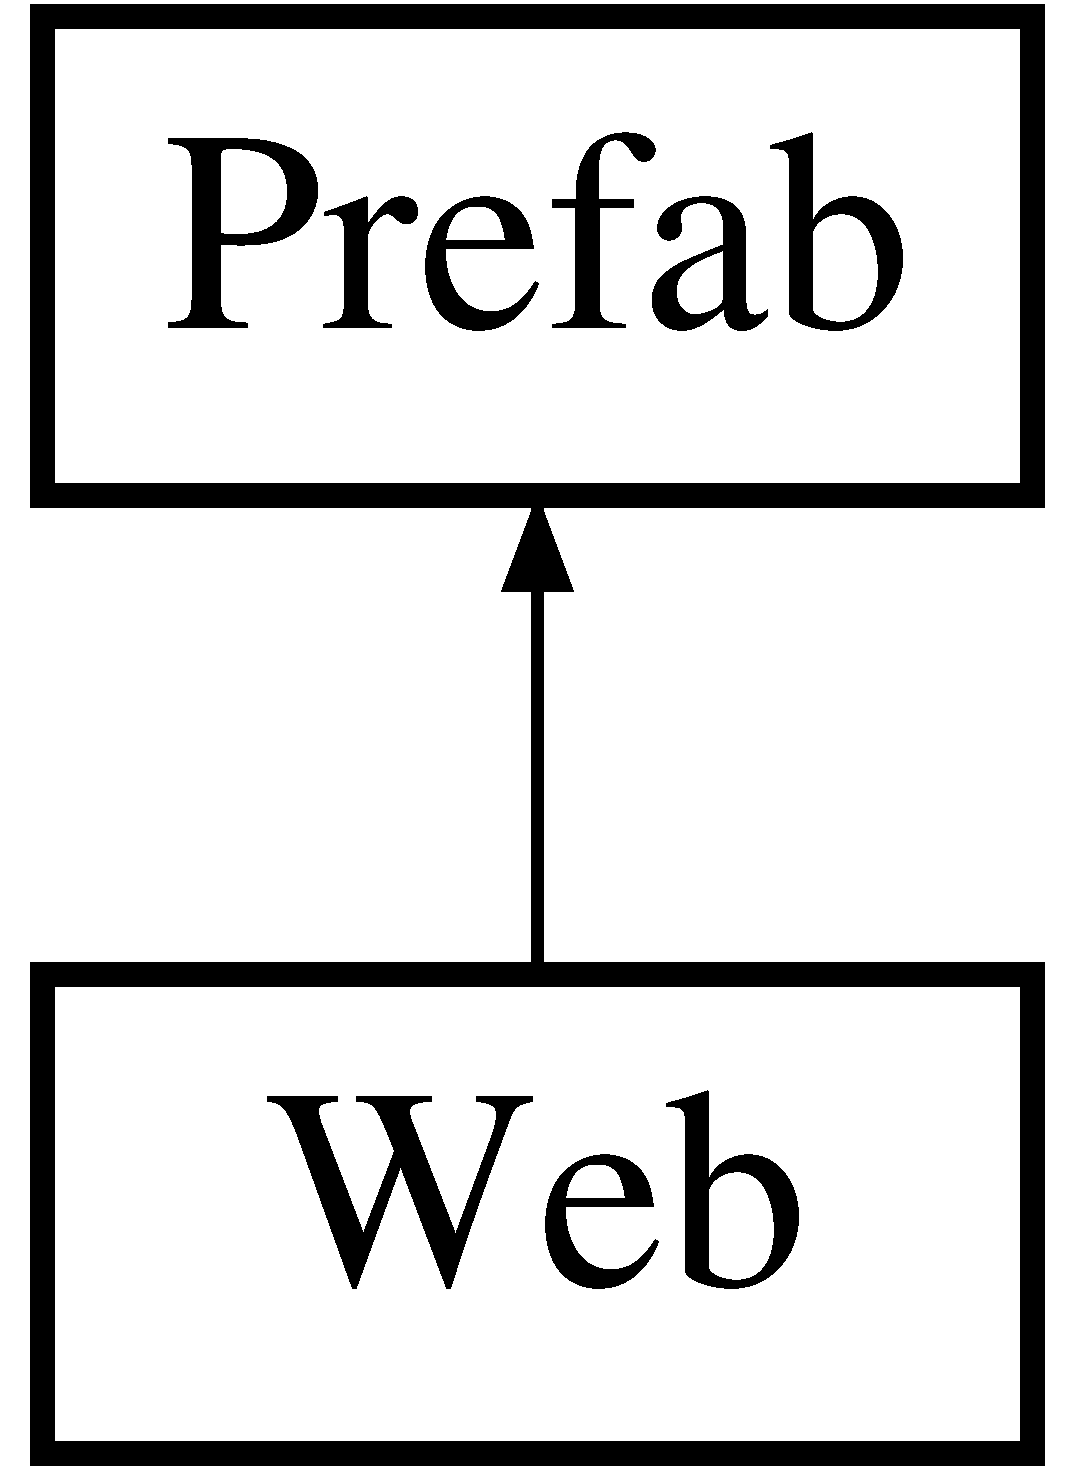
\includegraphics[height=2.000000cm]{class_web}
\end{center}
\end{figure}
\subsection*{Public Member Functions}
\begin{DoxyCompactItemize}
\item 
\hyperlink{class_web_a9cc4be82bd4865d5a006b4dd9fd174e5}{mime} (\$file)
\item 
\hyperlink{class_web_a67e70e21f07d54392cae50a140364268}{acceptable} (\$list=N\+U\+LL)
\item 
\hyperlink{class_web_a934eb97d44438943be35debae7302d8b}{send} (\$file, \$\hyperlink{class_web_a9cc4be82bd4865d5a006b4dd9fd174e5}{mime}=N\+U\+LL, \$kbps=0, \$force=T\+R\+UE, \$name=N\+U\+LL, \$flush=T\+R\+UE)
\item 
\hyperlink{class_web_a79336815638441bef6c31aa5961d88f0}{receive} (\$func=N\+U\+LL, \$overwrite=F\+A\+L\+SE, \$\hyperlink{class_web_a286c5e5759ec08bb103644e94de36b6f}{slug}=T\+R\+UE)
\item 
\hyperlink{class_web_a4a4e737abfbb551eb6c7ed583b042f93}{progress} (\$id)
\item 
\hyperlink{class_web_acf129dacf0ba4cb911f6573f8e24db54}{engine} (\$arg=\textquotesingle{}curl\textquotesingle{})
\item 
\hyperlink{class_web_acd091c5f2f55c3f0f5e1fce9dee1d76a}{subst} (array \&\$old, \$new)
\item 
\hyperlink{class_web_a65cd2273bee13f75e76463c5572e52ed}{request} (\$url, array \$options=N\+U\+LL)
\item 
\hyperlink{class_web_aa88be714af262e04d1468bf598880950}{minify} (\$files, \$\hyperlink{class_web_a9cc4be82bd4865d5a006b4dd9fd174e5}{mime}=N\+U\+LL, \$header=T\+R\+UE, \$path=N\+U\+LL)
\item 
\hyperlink{class_web_a6f4ec553292183f289c69a960578fe48}{rss} (\$url, \$max=10, \$tags=N\+U\+LL)
\item 
\hyperlink{class_web_acfaab3ed713ef4f5f14e1de378596d02}{whois} (\$addr, \$server=\textquotesingle{}whois.\+internic.\+net\textquotesingle{})
\item 
\hyperlink{class_web_a286c5e5759ec08bb103644e94de36b6f}{slug} (\$text)
\item 
\hyperlink{class_web_a0440b1db902b2ad8390cd1873c5aef76}{filler} (\$count=1, \$max=20, \$std=T\+R\+UE)
\end{DoxyCompactItemize}
\subsection*{Data Fields}
{\bf }\par
\begin{DoxyCompactItemize}
\item 
\hypertarget{class_web_a889c21a0ee6e7c0080976f8411dcba7f}{}\label{class_web_a889c21a0ee6e7c0080976f8411dcba7f} 
const {\bfseries E\+\_\+\+Request} =\textquotesingle{}No suitable H\+T\+TP \hyperlink{class_web_a65cd2273bee13f75e76463c5572e52ed}{request} \hyperlink{class_web_acf129dacf0ba4cb911f6573f8e24db54}{engine} found\textquotesingle{}
\end{DoxyCompactItemize}

\subsection*{Protected Member Functions}
\begin{DoxyCompactItemize}
\item 
\hyperlink{class_web_ace30d15b8ca06a3f846ccf20fc111beb}{\+\_\+curl} (\$url, \$options)
\item 
\hyperlink{class_web_ae9817da907b04f9d8e4fe307ef5180b8}{\+\_\+stream} (\$url, \$options)
\item 
\hyperlink{class_web_a9896cd454933a7743510844bd268b548}{\+\_\+socket} (\$url, \$options)
\end{DoxyCompactItemize}
\subsection*{Protected Attributes}
\begin{DoxyCompactItemize}
\item 
\hypertarget{class_web_ac0b1d0a2cca5e36ad2456397f4e2de6a}{}\label{class_web_ac0b1d0a2cca5e36ad2456397f4e2de6a} 
\hyperlink{class_web_ac0b1d0a2cca5e36ad2456397f4e2de6a}{\$wrapper}
\begin{DoxyCompactList}\small\item\em H\+T\+TP request engine. \end{DoxyCompactList}\end{DoxyCompactItemize}
\subsection*{Additional Inherited Members}


\subsection{Detailed Description}
Wrapper for various H\+T\+TP utilities. 

Definition at line 24 of file web.\+php.



\subsection{Member Function Documentation}
\hypertarget{class_web_ace30d15b8ca06a3f846ccf20fc111beb}{}\label{class_web_ace30d15b8ca06a3f846ccf20fc111beb} 
\index{Web@{Web}!\+\_\+curl@{\+\_\+curl}}
\index{\+\_\+curl@{\+\_\+curl}!Web@{Web}}
\subsubsection{\texorpdfstring{\+\_\+curl()}{\_curl()}}
{\footnotesize\ttfamily \+\_\+curl (\begin{DoxyParamCaption}\item[{}]{\$url,  }\item[{}]{\$options }\end{DoxyParamCaption})\hspace{0.3cm}{\ttfamily [protected]}}

H\+T\+TP request via c\+U\+RL \begin{DoxyReturn}{Returns}
array 
\end{DoxyReturn}

\begin{DoxyParams}{Parameters}
{\em \$url} & string \\
\hline
{\em \$options} & array \\
\hline
\end{DoxyParams}


Definition at line 263 of file web.\+php.

\hypertarget{class_web_a9896cd454933a7743510844bd268b548}{}\label{class_web_a9896cd454933a7743510844bd268b548} 
\index{Web@{Web}!\+\_\+socket@{\+\_\+socket}}
\index{\+\_\+socket@{\+\_\+socket}!Web@{Web}}
\subsubsection{\texorpdfstring{\+\_\+socket()}{\_socket()}}
{\footnotesize\ttfamily \+\_\+socket (\begin{DoxyParamCaption}\item[{}]{\$url,  }\item[{}]{\$options }\end{DoxyParamCaption})\hspace{0.3cm}{\ttfamily [protected]}}

H\+T\+TP request via low-\/level T\+C\+P/\+IP socket \begin{DoxyReturn}{Returns}
array 
\end{DoxyReturn}

\begin{DoxyParams}{Parameters}
{\em \$url} & string \\
\hline
{\em \$options} & array \\
\hline
\end{DoxyParams}


Definition at line 368 of file web.\+php.

\hypertarget{class_web_ae9817da907b04f9d8e4fe307ef5180b8}{}\label{class_web_ae9817da907b04f9d8e4fe307ef5180b8} 
\index{Web@{Web}!\+\_\+stream@{\+\_\+stream}}
\index{\+\_\+stream@{\+\_\+stream}!Web@{Web}}
\subsubsection{\texorpdfstring{\+\_\+stream()}{\_stream()}}
{\footnotesize\ttfamily \+\_\+stream (\begin{DoxyParamCaption}\item[{}]{\$url,  }\item[{}]{\$options }\end{DoxyParamCaption})\hspace{0.3cm}{\ttfamily [protected]}}

H\+T\+TP request via P\+HP stream wrapper \begin{DoxyReturn}{Returns}
array 
\end{DoxyReturn}

\begin{DoxyParams}{Parameters}
{\em \$url} & string \\
\hline
{\em \$options} & array \\
\hline
\end{DoxyParams}


Definition at line 326 of file web.\+php.

\hypertarget{class_web_a67e70e21f07d54392cae50a140364268}{}\label{class_web_a67e70e21f07d54392cae50a140364268} 
\index{Web@{Web}!acceptable@{acceptable}}
\index{acceptable@{acceptable}!Web@{Web}}
\subsubsection{\texorpdfstring{acceptable()}{acceptable()}}
{\footnotesize\ttfamily acceptable (\begin{DoxyParamCaption}\item[{}]{\$list = {\ttfamily NULL} }\end{DoxyParamCaption})}

Return the M\+I\+ME types stated in the H\+T\+TP Accept header as an array; If a list of M\+I\+ME types is specified, return the best match; or F\+A\+L\+SE if none found \begin{DoxyReturn}{Returns}
array$\vert$string$\vert$\+F\+A\+L\+SE 
\end{DoxyReturn}

\begin{DoxyParams}{Parameters}
{\em \$list} & string$\vert$array \\
\hline
\end{DoxyParams}


Definition at line 95 of file web.\+php.

\hypertarget{class_web_acf129dacf0ba4cb911f6573f8e24db54}{}\label{class_web_acf129dacf0ba4cb911f6573f8e24db54} 
\index{Web@{Web}!engine@{engine}}
\index{engine@{engine}!Web@{Web}}
\subsubsection{\texorpdfstring{engine()}{engine()}}
{\footnotesize\ttfamily engine (\begin{DoxyParamCaption}\item[{}]{\$arg = {\ttfamily \textquotesingle{}curl\textquotesingle{}} }\end{DoxyParamCaption})}

Specify the H\+T\+TP request engine to use; If not available, fall back to an applicable substitute \begin{DoxyReturn}{Returns}
string 
\end{DoxyReturn}

\begin{DoxyParams}{Parameters}
{\em \$arg} & string \\
\hline
\end{DoxyParams}


Definition at line 441 of file web.\+php.

\hypertarget{class_web_a0440b1db902b2ad8390cd1873c5aef76}{}\label{class_web_a0440b1db902b2ad8390cd1873c5aef76} 
\index{Web@{Web}!filler@{filler}}
\index{filler@{filler}!Web@{Web}}
\subsubsection{\texorpdfstring{filler()}{filler()}}
{\footnotesize\ttfamily filler (\begin{DoxyParamCaption}\item[{}]{\$count = {\ttfamily 1},  }\item[{}]{\$max = {\ttfamily 20},  }\item[{}]{\$std = {\ttfamily TRUE} }\end{DoxyParamCaption})}

Return chunk of text from standard Lorem Ipsum passage \begin{DoxyReturn}{Returns}
string 
\end{DoxyReturn}

\begin{DoxyParams}{Parameters}
{\em \$count} & int \\
\hline
{\em \$max} & int \\
\hline
{\em \$std} & bool \\
\hline
\end{DoxyParams}


Definition at line 835 of file web.\+php.

\hypertarget{class_web_a9cc4be82bd4865d5a006b4dd9fd174e5}{}\label{class_web_a9cc4be82bd4865d5a006b4dd9fd174e5} 
\index{Web@{Web}!mime@{mime}}
\index{mime@{mime}!Web@{Web}}
\subsubsection{\texorpdfstring{mime()}{mime()}}
{\footnotesize\ttfamily mime (\begin{DoxyParamCaption}\item[{}]{\$file }\end{DoxyParamCaption})}

Detect M\+I\+ME type using file extension \begin{DoxyReturn}{Returns}
string 
\end{DoxyReturn}

\begin{DoxyParams}{Parameters}
{\em \$file} & string \\
\hline
\end{DoxyParams}


Definition at line 40 of file web.\+php.

\hypertarget{class_web_aa88be714af262e04d1468bf598880950}{}\label{class_web_aa88be714af262e04d1468bf598880950} 
\index{Web@{Web}!minify@{minify}}
\index{minify@{minify}!Web@{Web}}
\subsubsection{\texorpdfstring{minify()}{minify()}}
{\footnotesize\ttfamily minify (\begin{DoxyParamCaption}\item[{}]{\$files,  }\item[{}]{\$mime = {\ttfamily NULL},  }\item[{}]{\$header = {\ttfamily TRUE},  }\item[{}]{\$path = {\ttfamily NULL} }\end{DoxyParamCaption})}

Strip Javascript/\+C\+SS files of extraneous whitespaces and comments; Return combined output as a minified string \begin{DoxyReturn}{Returns}
string 
\end{DoxyReturn}

\begin{DoxyParams}{Parameters}
{\em \$files} & string$\vert$array \\
\hline
{\em \$mime} & string \\
\hline
{\em \$header} & bool \\
\hline
{\em \$path} & string \\
\hline
\end{DoxyParams}


Definition at line 577 of file web.\+php.

\hypertarget{class_web_a4a4e737abfbb551eb6c7ed583b042f93}{}\label{class_web_a4a4e737abfbb551eb6c7ed583b042f93} 
\index{Web@{Web}!progress@{progress}}
\index{progress@{progress}!Web@{Web}}
\subsubsection{\texorpdfstring{progress()}{progress()}}
{\footnotesize\ttfamily progress (\begin{DoxyParamCaption}\item[{}]{\$id }\end{DoxyParamCaption})}

Return upload progress in bytes, F\+A\+L\+SE on failure \begin{DoxyReturn}{Returns}
int$\vert$\+F\+A\+L\+SE 
\end{DoxyReturn}

\begin{DoxyParams}{Parameters}
{\em \$id} & string \\
\hline
\end{DoxyParams}


Definition at line 250 of file web.\+php.

\hypertarget{class_web_a79336815638441bef6c31aa5961d88f0}{}\label{class_web_a79336815638441bef6c31aa5961d88f0} 
\index{Web@{Web}!receive@{receive}}
\index{receive@{receive}!Web@{Web}}
\subsubsection{\texorpdfstring{receive()}{receive()}}
{\footnotesize\ttfamily receive (\begin{DoxyParamCaption}\item[{}]{\$func = {\ttfamily NULL},  }\item[{}]{\$overwrite = {\ttfamily FALSE},  }\item[{}]{\$slug = {\ttfamily TRUE} }\end{DoxyParamCaption})}

Receive file(s) from H\+T\+TP client \begin{DoxyReturn}{Returns}
array$\vert$bool 
\end{DoxyReturn}

\begin{DoxyParams}{Parameters}
{\em \$func} & callback \\
\hline
{\em \$overwrite} & bool \\
\hline
{\em \$slug} & callback$\vert$bool \\
\hline
\end{DoxyParams}


Definition at line 173 of file web.\+php.

\hypertarget{class_web_a65cd2273bee13f75e76463c5572e52ed}{}\label{class_web_a65cd2273bee13f75e76463c5572e52ed} 
\index{Web@{Web}!request@{request}}
\index{request@{request}!Web@{Web}}
\subsubsection{\texorpdfstring{request()}{request()}}
{\footnotesize\ttfamily request (\begin{DoxyParamCaption}\item[{}]{\$url,  }\item[{array}]{\$options = {\ttfamily NULL} }\end{DoxyParamCaption})}

Submit H\+T\+TP request; Use H\+T\+TP context options (described in \href{http://www.php.net/manual/en/context.http.php}{\tt http\+://www.\+php.\+net/manual/en/context.\+http.\+php}) if specified; \hyperlink{class_cache}{Cache} the page as instructed by remote server \begin{DoxyReturn}{Returns}
array$\vert$\+F\+A\+L\+SE 
\end{DoxyReturn}

\begin{DoxyParams}{Parameters}
{\em \$url} & string \\
\hline
{\em \$options} & array \\
\hline
\end{DoxyParams}


Definition at line 480 of file web.\+php.

\hypertarget{class_web_a6f4ec553292183f289c69a960578fe48}{}\label{class_web_a6f4ec553292183f289c69a960578fe48} 
\index{Web@{Web}!rss@{rss}}
\index{rss@{rss}!Web@{Web}}
\subsubsection{\texorpdfstring{rss()}{rss()}}
{\footnotesize\ttfamily rss (\begin{DoxyParamCaption}\item[{}]{\$url,  }\item[{}]{\$max = {\ttfamily 10},  }\item[{}]{\$tags = {\ttfamily NULL} }\end{DoxyParamCaption})}

Retrieve R\+SS feed and return as an array \begin{DoxyReturn}{Returns}
array$\vert$\+F\+A\+L\+SE 
\end{DoxyReturn}

\begin{DoxyParams}{Parameters}
{\em \$url} & string \\
\hline
{\em \$max} & int \\
\hline
{\em \$tags} & string \\
\hline
\end{DoxyParams}


Definition at line 713 of file web.\+php.

\hypertarget{class_web_a934eb97d44438943be35debae7302d8b}{}\label{class_web_a934eb97d44438943be35debae7302d8b} 
\index{Web@{Web}!send@{send}}
\index{send@{send}!Web@{Web}}
\subsubsection{\texorpdfstring{send()}{send()}}
{\footnotesize\ttfamily send (\begin{DoxyParamCaption}\item[{}]{\$file,  }\item[{}]{\$mime = {\ttfamily NULL},  }\item[{}]{\$kbps = {\ttfamily 0},  }\item[{}]{\$force = {\ttfamily TRUE},  }\item[{}]{\$name = {\ttfamily NULL},  }\item[{}]{\$flush = {\ttfamily TRUE} }\end{DoxyParamCaption})}

Transmit file to H\+T\+TP client; Return file size if successful, F\+A\+L\+SE otherwise \begin{DoxyReturn}{Returns}
int$\vert$\+F\+A\+L\+SE 
\end{DoxyReturn}

\begin{DoxyParams}{Parameters}
{\em \$file} & string \\
\hline
{\em \$mime} & string \\
\hline
{\em \$kbps} & int \\
\hline
{\em \$force} & bool \\
\hline
{\em \$name} & string \\
\hline
{\em \$flush} & bool \\
\hline
\end{DoxyParams}


Definition at line 130 of file web.\+php.

\hypertarget{class_web_a286c5e5759ec08bb103644e94de36b6f}{}\label{class_web_a286c5e5759ec08bb103644e94de36b6f} 
\index{Web@{Web}!slug@{slug}}
\index{slug@{slug}!Web@{Web}}
\subsubsection{\texorpdfstring{slug()}{slug()}}
{\footnotesize\ttfamily slug (\begin{DoxyParamCaption}\item[{}]{\$text }\end{DoxyParamCaption})}

Return a U\+R\+L/filesystem-\/friendly version of string \begin{DoxyReturn}{Returns}
string 
\end{DoxyReturn}

\begin{DoxyParams}{Parameters}
{\em \$text} & string \\
\hline
\end{DoxyParams}


Definition at line 774 of file web.\+php.

\hypertarget{class_web_acd091c5f2f55c3f0f5e1fce9dee1d76a}{}\label{class_web_acd091c5f2f55c3f0f5e1fce9dee1d76a} 
\index{Web@{Web}!subst@{subst}}
\index{subst@{subst}!Web@{Web}}
\subsubsection{\texorpdfstring{subst()}{subst()}}
{\footnotesize\ttfamily subst (\begin{DoxyParamCaption}\item[{array \&}]{\$old,  }\item[{}]{\$new }\end{DoxyParamCaption})}

Replace old headers with new elements \begin{DoxyReturn}{Returns}
N\+U\+LL 
\end{DoxyReturn}

\begin{DoxyParams}{Parameters}
{\em \$old} & array \\
\hline
{\em \$new} & string$\vert$array \\
\hline
\end{DoxyParams}


Definition at line 462 of file web.\+php.

\hypertarget{class_web_acfaab3ed713ef4f5f14e1de378596d02}{}\label{class_web_acfaab3ed713ef4f5f14e1de378596d02} 
\index{Web@{Web}!whois@{whois}}
\index{whois@{whois}!Web@{Web}}
\subsubsection{\texorpdfstring{whois()}{whois()}}
{\footnotesize\ttfamily whois (\begin{DoxyParamCaption}\item[{}]{\$addr,  }\item[{}]{\$server = {\ttfamily \textquotesingle{}whois.internic.net\textquotesingle{}} }\end{DoxyParamCaption})}

Retrieve information from whois server \begin{DoxyReturn}{Returns}
string$\vert$\+F\+A\+L\+SE 
\end{DoxyReturn}

\begin{DoxyParams}{Parameters}
{\em \$addr} & string \\
\hline
{\em \$server} & string \\
\hline
\end{DoxyParams}


Definition at line 748 of file web.\+php.



The documentation for this class was generated from the following file\+:\begin{DoxyCompactItemize}
\item 
/\+Users/aplennevaux/\+G\+I\+T\+H\+U\+B/\+Visionary-\/website/src/vendor/bcosca/fatfree/lib/web.\+php\end{DoxyCompactItemize}

\hypertarget{class_c_l_i_1_1_w_s}{}\section{WS Class Reference}
\label{class_c_l_i_1_1_w_s}\index{WS@{WS}}


R\+F\+C6455 Web\+Socket server.  


\subsection*{Public Member Functions}
\begin{DoxyCompactItemize}
\item 
\hyperlink{class_c_l_i_1_1_w_s_a201f40e4b8683b5e569b4c1e8add9fcd}{alloc} (\$socket)
\item 
\hyperlink{class_c_l_i_1_1_w_s_aa3a3bd26af1b767091f521a6c9041e56}{close} (\$socket)
\item 
\hyperlink{class_c_l_i_1_1_w_s_a6b8891e0c2b12c863512071111b9aa07}{free} (\$socket)
\item 
\hyperlink{class_c_l_i_1_1_w_s_a845d775219b4327eb7cb626ffb1c2af3}{read} (\$socket)
\item 
\hyperlink{class_c_l_i_1_1_w_s_ac95ce2fb30c44bae1927b0107756f7e3}{write} (\$socket, \$str)
\item 
\hyperlink{class_c_l_i_1_1_w_s_a5c3b4aef24eacefe766d9e34fd5791de}{agents} (\$uri=N\+U\+LL)
\item 
\hyperlink{class_c_l_i_1_1_w_s_ade509b07f1df45730d31589b81a26efb}{events} ()
\item 
\hyperlink{class_c_l_i_1_1_w_s_a65a51fe8cfc1c6b4d04178b209b50e23}{on} (\$event, \$func)
\item 
\hyperlink{class_c_l_i_1_1_w_s_a2e5652a68528b58bda9e63311cd473bd}{kill} (\$signal)
\item 
\hyperlink{class_c_l_i_1_1_w_s_afb0fafe7e02a3ae1993c01c19fad2bae}{run} ()
\item 
\hyperlink{class_c_l_i_1_1_w_s_a19dbb10de3a82395f1c941e3f37fe8c7}{\+\_\+\+\_\+construct} (\$addr, \$ctx=N\+U\+LL, \$wait=60)
\end{DoxyCompactItemize}
\subsection*{Data Fields}
\begin{DoxyCompactItemize}
\item 
\hypertarget{class_c_l_i_1_1_w_s_a0f8417d2e128a6f19f2b5e0a0a883de0}{}\label{class_c_l_i_1_1_w_s_a0f8417d2e128a6f19f2b5e0a0a883de0} 
const \hyperlink{class_c_l_i_1_1_w_s_a0f8417d2e128a6f19f2b5e0a0a883de0}{Magic} =\textquotesingle{}258\+E\+A\+F\+A5-\/\+E914-\/47\+D\+A-\/95\+C\+A-\/\+C5\+A\+B0\+D\+C85\+B11\textquotesingle{}
\begin{DoxyCompactList}\small\item\em U\+U\+ID magic string. \end{DoxyCompactList}\item 
\hypertarget{class_c_l_i_1_1_w_s_adbc81c45b48c6cdfffe9fc4752007493}{}\label{class_c_l_i_1_1_w_s_adbc81c45b48c6cdfffe9fc4752007493} 
const \hyperlink{class_c_l_i_1_1_w_s_adbc81c45b48c6cdfffe9fc4752007493}{Packet} =65536
\begin{DoxyCompactList}\small\item\em Max packet size. \end{DoxyCompactList}\item 
\hypertarget{class_c_l_i_1_1_w_s_aa0f7bf6b5a60518284ef88fa33e264f2}{}\label{class_c_l_i_1_1_w_s_aa0f7bf6b5a60518284ef88fa33e264f2} 
{\bfseries \$ctx}
\item 
\hypertarget{class_c_l_i_1_1_w_s_a165566db3c2de8a5e20d0957ed606e46}{}\label{class_c_l_i_1_1_w_s_a165566db3c2de8a5e20d0957ed606e46} 
{\bfseries \$wait}
\item 
\hypertarget{class_c_l_i_1_1_w_s_a4faf536a5ff25a28adb9891716556dc6}{}\label{class_c_l_i_1_1_w_s_a4faf536a5ff25a28adb9891716556dc6} 
{\bfseries \$sockets}
\item 
\hypertarget{class_c_l_i_1_1_w_s_af8624bfcd6ccf58a6906baf72ec078df}{}\label{class_c_l_i_1_1_w_s_af8624bfcd6ccf58a6906baf72ec078df} 
{\bfseries \$agents} =\mbox{[}$\,$\mbox{]}
\item 
\hypertarget{class_c_l_i_1_1_w_s_a1bcec9bbd34255927faaf155bf3a940a}{}\label{class_c_l_i_1_1_w_s_a1bcec9bbd34255927faaf155bf3a940a} 
{\bfseries \$events} =\mbox{[}$\,$\mbox{]}
\end{DoxyCompactItemize}
{\bf }\par
\begin{DoxyCompactItemize}
\item 
\hypertarget{class_c_l_i_1_1_w_s_aa9141b93fff959a11eb401b7100b7a90}{}\label{class_c_l_i_1_1_w_s_aa9141b93fff959a11eb401b7100b7a90} 
const {\bfseries Text} =0x01
\item 
\hypertarget{class_c_l_i_1_1_w_s_a03a9c4aa0f0905b7512a268997cbe41f}{}\label{class_c_l_i_1_1_w_s_a03a9c4aa0f0905b7512a268997cbe41f} 
const {\bfseries Binary} =0x02
\item 
\hypertarget{class_c_l_i_1_1_w_s_a12592aa7eb9f1570fc962867a7fcc904}{}\label{class_c_l_i_1_1_w_s_a12592aa7eb9f1570fc962867a7fcc904} 
const {\bfseries Close} =0x08
\item 
\hypertarget{class_c_l_i_1_1_w_s_ad953baab1d22f9595927e18f6ac8ec16}{}\label{class_c_l_i_1_1_w_s_ad953baab1d22f9595927e18f6ac8ec16} 
const {\bfseries Ping} =0x09
\item 
\hypertarget{class_c_l_i_1_1_w_s_a969c5d07e26af01d3523ec69379a4df5}{}\label{class_c_l_i_1_1_w_s_a969c5d07e26af01d3523ec69379a4df5} 
const {\bfseries Pong} =0x0a
\item 
\hypertarget{class_c_l_i_1_1_w_s_af8603b6923a1a089b57cb849bc062148}{}\label{class_c_l_i_1_1_w_s_af8603b6923a1a089b57cb849bc062148} 
const {\bfseries Op\+Code} =0x0f
\item 
\hypertarget{class_c_l_i_1_1_w_s_afa14d696444a689a5be47c64ce568983}{}\label{class_c_l_i_1_1_w_s_afa14d696444a689a5be47c64ce568983} 
const {\bfseries Finale} =0x80
\end{DoxyCompactItemize}

{\bf }\par
\begin{DoxyCompactItemize}
\item 
\hypertarget{class_c_l_i_1_1_w_s_a62a38e46cf476443cf933907fe86e684}{}\label{class_c_l_i_1_1_w_s_a62a38e46cf476443cf933907fe86e684} 
const {\bfseries Length} =0x7f
\end{DoxyCompactItemize}

\subsection*{Protected Attributes}
\begin{DoxyCompactItemize}
\item 
\hypertarget{class_c_l_i_1_1_w_s_a80e1c53e5ae106ed41bc69db8cdcdf78}{}\label{class_c_l_i_1_1_w_s_a80e1c53e5ae106ed41bc69db8cdcdf78} 
{\bfseries \$addr}
\end{DoxyCompactItemize}


\subsection{Detailed Description}
R\+F\+C6455 Web\+Socket server. 

Definition at line 26 of file ws.\+php.



\subsection{Constructor \& Destructor Documentation}
\hypertarget{class_c_l_i_1_1_w_s_a19dbb10de3a82395f1c941e3f37fe8c7}{}\label{class_c_l_i_1_1_w_s_a19dbb10de3a82395f1c941e3f37fe8c7} 
\index{C\+L\+I\+::\+WS@{C\+L\+I\+::\+WS}!\+\_\+\+\_\+construct@{\+\_\+\+\_\+construct}}
\index{\+\_\+\+\_\+construct@{\+\_\+\+\_\+construct}!C\+L\+I\+::\+WS@{C\+L\+I\+::\+WS}}
\subsubsection{\texorpdfstring{\+\_\+\+\_\+construct()}{\_\_construct()}}
{\footnotesize\ttfamily \+\_\+\+\_\+construct (\begin{DoxyParamCaption}\item[{}]{\$addr,  }\item[{}]{\$ctx = {\ttfamily NULL},  }\item[{}]{\$wait = {\ttfamily 60} }\end{DoxyParamCaption})}

Instantiate object \begin{DoxyReturn}{Returns}
object 
\end{DoxyReturn}

\begin{DoxyParams}{Parameters}
{\em \$addr} & string \\
\hline
{\em \$ctx} & resource \\
\hline
{\em \$wait} & int \\
\hline
\end{DoxyParams}


Definition at line 345 of file ws.\+php.



\subsection{Member Function Documentation}
\hypertarget{class_c_l_i_1_1_w_s_a5c3b4aef24eacefe766d9e34fd5791de}{}\label{class_c_l_i_1_1_w_s_a5c3b4aef24eacefe766d9e34fd5791de} 
\index{C\+L\+I\+::\+WS@{C\+L\+I\+::\+WS}!agents@{agents}}
\index{agents@{agents}!C\+L\+I\+::\+WS@{C\+L\+I\+::\+WS}}
\subsubsection{\texorpdfstring{agents()}{agents()}}
{\footnotesize\ttfamily agents (\begin{DoxyParamCaption}\item[{}]{\$uri = {\ttfamily NULL} }\end{DoxyParamCaption})}

Return socket agents \begin{DoxyReturn}{Returns}
array 
\end{DoxyReturn}

\begin{DoxyParams}{Parameters}
{\em \$uri} & string \\
\hline
\end{DoxyParams}


Definition at line 193 of file ws.\+php.

\hypertarget{class_c_l_i_1_1_w_s_a201f40e4b8683b5e569b4c1e8add9fcd}{}\label{class_c_l_i_1_1_w_s_a201f40e4b8683b5e569b4c1e8add9fcd} 
\index{C\+L\+I\+::\+WS@{C\+L\+I\+::\+WS}!alloc@{alloc}}
\index{alloc@{alloc}!C\+L\+I\+::\+WS@{C\+L\+I\+::\+WS}}
\subsubsection{\texorpdfstring{alloc()}{alloc()}}
{\footnotesize\ttfamily alloc (\begin{DoxyParamCaption}\item[{}]{\$socket }\end{DoxyParamCaption})}

Allocate stream socket \begin{DoxyReturn}{Returns}
N\+U\+LL 
\end{DoxyReturn}

\begin{DoxyParams}{Parameters}
{\em \$socket} & resource \\
\hline
\end{DoxyParams}


Definition at line 63 of file ws.\+php.

\hypertarget{class_c_l_i_1_1_w_s_aa3a3bd26af1b767091f521a6c9041e56}{}\label{class_c_l_i_1_1_w_s_aa3a3bd26af1b767091f521a6c9041e56} 
\index{C\+L\+I\+::\+WS@{C\+L\+I\+::\+WS}!close@{close}}
\index{close@{close}!C\+L\+I\+::\+WS@{C\+L\+I\+::\+WS}}
\subsubsection{\texorpdfstring{close()}{close()}}
{\footnotesize\ttfamily close (\begin{DoxyParamCaption}\item[{}]{\$socket }\end{DoxyParamCaption})}

Close stream socket \begin{DoxyReturn}{Returns}
N\+U\+LL 
\end{DoxyReturn}

\begin{DoxyParams}{Parameters}
{\em \$socket} & resource \\
\hline
\end{DoxyParams}


Definition at line 137 of file ws.\+php.

\hypertarget{class_c_l_i_1_1_w_s_ade509b07f1df45730d31589b81a26efb}{}\label{class_c_l_i_1_1_w_s_ade509b07f1df45730d31589b81a26efb} 
\index{C\+L\+I\+::\+WS@{C\+L\+I\+::\+WS}!events@{events}}
\index{events@{events}!C\+L\+I\+::\+WS@{C\+L\+I\+::\+WS}}
\subsubsection{\texorpdfstring{events()}{events()}}
{\footnotesize\ttfamily events (\begin{DoxyParamCaption}{ }\end{DoxyParamCaption})}

Return event handlers \begin{DoxyReturn}{Returns}
array 
\end{DoxyReturn}


Definition at line 206 of file ws.\+php.

\hypertarget{class_c_l_i_1_1_w_s_a6b8891e0c2b12c863512071111b9aa07}{}\label{class_c_l_i_1_1_w_s_a6b8891e0c2b12c863512071111b9aa07} 
\index{C\+L\+I\+::\+WS@{C\+L\+I\+::\+WS}!free@{free}}
\index{free@{free}!C\+L\+I\+::\+WS@{C\+L\+I\+::\+WS}}
\subsubsection{\texorpdfstring{free()}{free()}}
{\footnotesize\ttfamily free (\begin{DoxyParamCaption}\item[{}]{\$socket }\end{DoxyParamCaption})}

Free stream socket \begin{DoxyReturn}{Returns}
bool 
\end{DoxyReturn}

\begin{DoxyParams}{Parameters}
{\em \$socket} & resource \\
\hline
\end{DoxyParams}


Definition at line 147 of file ws.\+php.

\hypertarget{class_c_l_i_1_1_w_s_a2e5652a68528b58bda9e63311cd473bd}{}\label{class_c_l_i_1_1_w_s_a2e5652a68528b58bda9e63311cd473bd} 
\index{C\+L\+I\+::\+WS@{C\+L\+I\+::\+WS}!kill@{kill}}
\index{kill@{kill}!C\+L\+I\+::\+WS@{C\+L\+I\+::\+WS}}
\subsubsection{\texorpdfstring{kill()}{kill()}}
{\footnotesize\ttfamily kill (\begin{DoxyParamCaption}\item[{}]{\$signal }\end{DoxyParamCaption})}

Terminate server \begin{DoxyReturn}{Returns}
N\+U\+LL 
\end{DoxyReturn}

\begin{DoxyParams}{Parameters}
{\em \$signal} & int \\
\hline
\end{DoxyParams}


Definition at line 226 of file ws.\+php.

\hypertarget{class_c_l_i_1_1_w_s_a65a51fe8cfc1c6b4d04178b209b50e23}{}\label{class_c_l_i_1_1_w_s_a65a51fe8cfc1c6b4d04178b209b50e23} 
\index{C\+L\+I\+::\+WS@{C\+L\+I\+::\+WS}!on@{on}}
\index{on@{on}!C\+L\+I\+::\+WS@{C\+L\+I\+::\+WS}}
\subsubsection{\texorpdfstring{on()}{on()}}
{\footnotesize\ttfamily on (\begin{DoxyParamCaption}\item[{}]{\$event,  }\item[{}]{\$func }\end{DoxyParamCaption})}

Bind function to event handler \begin{DoxyReturn}{Returns}
object 
\end{DoxyReturn}

\begin{DoxyParams}{Parameters}
{\em \$event} & string \\
\hline
{\em \$func} & callable \\
\hline
\end{DoxyParams}


Definition at line 216 of file ws.\+php.

\hypertarget{class_c_l_i_1_1_w_s_a845d775219b4327eb7cb626ffb1c2af3}{}\label{class_c_l_i_1_1_w_s_a845d775219b4327eb7cb626ffb1c2af3} 
\index{C\+L\+I\+::\+WS@{C\+L\+I\+::\+WS}!read@{read}}
\index{read@{read}!C\+L\+I\+::\+WS@{C\+L\+I\+::\+WS}}
\subsubsection{\texorpdfstring{read()}{read()}}
{\footnotesize\ttfamily read (\begin{DoxyParamCaption}\item[{}]{\$socket }\end{DoxyParamCaption})}

Read from stream socket \begin{DoxyReturn}{Returns}
string$\vert$\+F\+A\+L\+SE 
\end{DoxyReturn}

\begin{DoxyParams}{Parameters}
{\em \$socket} & resource \\
\hline
\end{DoxyParams}


Definition at line 158 of file ws.\+php.

\hypertarget{class_c_l_i_1_1_w_s_afb0fafe7e02a3ae1993c01c19fad2bae}{}\label{class_c_l_i_1_1_w_s_afb0fafe7e02a3ae1993c01c19fad2bae} 
\index{C\+L\+I\+::\+WS@{C\+L\+I\+::\+WS}!run@{run}}
\index{run@{run}!C\+L\+I\+::\+WS@{C\+L\+I\+::\+WS}}
\subsubsection{\texorpdfstring{run()}{run()}}
{\footnotesize\ttfamily run (\begin{DoxyParamCaption}{ }\end{DoxyParamCaption})}

Execute the server process \begin{DoxyReturn}{Returns}
object 
\end{DoxyReturn}


Definition at line 234 of file ws.\+php.

\hypertarget{class_c_l_i_1_1_w_s_ac95ce2fb30c44bae1927b0107756f7e3}{}\label{class_c_l_i_1_1_w_s_ac95ce2fb30c44bae1927b0107756f7e3} 
\index{C\+L\+I\+::\+WS@{C\+L\+I\+::\+WS}!write@{write}}
\index{write@{write}!C\+L\+I\+::\+WS@{C\+L\+I\+::\+WS}}
\subsubsection{\texorpdfstring{write()}{write()}}
{\footnotesize\ttfamily write (\begin{DoxyParamCaption}\item[{}]{\$socket,  }\item[{}]{\$str }\end{DoxyParamCaption})}

Write to stream socket \begin{DoxyReturn}{Returns}
int$\vert$\+F\+A\+L\+SE 
\end{DoxyReturn}

\begin{DoxyParams}{Parameters}
{\em \$socket} & resource \\
\hline
{\em \$str} & string \\
\hline
\end{DoxyParams}


Definition at line 175 of file ws.\+php.



The documentation for this class was generated from the following file\+:\begin{DoxyCompactItemize}
\item 
/\+Users/aplennevaux/\+G\+I\+T\+H\+U\+B/\+Visionary-\/website/src/vendor/bcosca/fatfree/lib/cli/ws.\+php\end{DoxyCompactItemize}

%--- End generated contents ---

% Index
\backmatter
\newpage
\phantomsection
\clearemptydoublepage
\addcontentsline{toc}{chapter}{Index}
\printindex

\end{document}
